\documentclass[cyan]{elegantnote}
\author{Yuyang Songsheng}
\email{songshengyuyang@gmail.com}
\zhtitle{物理}
\entitle{Physics}
\version{1.00}
\myquote{Summary is the best way to say ``Good Bye''}
\logo{logo.jpg}
\cover{cover.pdf}
%green color
   \definecolor{main1}{RGB}{210,168,75}
   \definecolor{seco1}{RGB}{9,80,3}
   \definecolor{thid1}{RGB}{0,175,152}
%cyan color
   \definecolor{main2}{RGB}{239,126,30}
   \definecolor{seco2}{RGB}{0,175,152}
   \definecolor{thid2}{RGB}{236,74,53}
%cyan color
   \definecolor{main3}{RGB}{127,191,51}
   \definecolor{seco3}{RGB}{0,145,215}
   \definecolor{thid3}{RGB}{180,27,131}

\usepackage{mhchem}
\usepackage{makecell}
\usepackage{lipsum}
\usepackage{amssymb}
\usepackage{float}
\usepackage{wrapfig}
\usepackage{latexsym}
\usepackage{hyperref}
\usepackage{feynmf}
\usepackage{exscale}
\usepackage{relsize}
\usepackage{slashed}
\usepackage{mathrsfs}
\usepackage{tensor}
\usepackage{bm}%bold math, for vector

\begin{document}
\maketitle
\tableofcontents
\part{Classical Mechanics}
\chapter{The Formulation of Classical Mechanics}
\section{Lagrangian formulation}
\[S=\int_{t_1}^{t_2}L(q_i,\dot{q_i},t)dt, \ \ \ \ \delta q_i(t_1) = \delta q_i(t_2) = 0.\]
\[\delta S=0 \rightarrow \frac{d}{dt}(\frac{\partial L}{\partial \dot{q_i}}) - \frac{\partial L}{\partial q_i}=0.\]

\begin{enumerate}
\item If we transform the coordinates $q$ to the $Q$ as $q = q(Q,t)$, the new Lagrangian will be
\[\bar{L}(Q,\dot{Q},t) \equiv L(q(Q,t),\dot{q}(Q,\dot{Q},t),t).\]
We can verify that
\[\frac{d}{dt}\frac{\partial \bar{L}}{\partial \dot{Q}} - \frac{\partial \bar{L}}{\partial Q} = 0.\]
\item If $L_1 = L + \frac{d}{dt} f(q,t)$, then $L$ and $L_1$ is equivalent and will generate the same dynamical equation.
\end{enumerate}

\begin{example}
\begin{enumerate}
\item The form of Lagrangian for an isolated system of particles in inertial frame:
\[L=\sum_a \frac{1}{2}m_a v_a^2 -U(\bm{r}_1,\bm{r}_2,\cdots).\]
The equation of motion is
\[m_i \ddot{\bm{r}}_i = -\nabla_{\bm{r}_i} U.\]
To get the form of Lagrangian for a system of interacting particles, we must assume:
\begin{itemize}
\item Space and time are homogeneous and isotropic in inertial frame;
\item Galileo's relativity principle and Galilean transformation;
\item Spontaneous interaction between particles;
\end{itemize}
\item Consider a reference frame $K$. Suppose the $K$ is moving with the velocity $\bm{V}(t)$ and  rotating with angular velocity $\bm{\Omega}$  relative to the inertial reference frame. We use the coordinates of the mass point in $K$ as general coordinates, i.e. $\bm{r} = (x_k,y_k,z_k)$. Then the Lagrangian of the mass point will be
\[L = \frac{1}{2}m\bm{v}^2 + m\bm{v}\cdot(\bm{\Omega}\times\bm{r})+\frac{m}{2}(\bm{\Omega}\times\bm{r})^2 - m\dot{\bm{V}}\cdot\bm{r}-U.\]
The equation of motion will be
\[m\frac{d\bm{v}}{dt} = -\frac{\partial U}{\partial \bm{r}} - m\dot{\bm{V}} + m(\bm{r} \times \dot{\bm{\Omega}}) + 2m(\bm{v} \times \bm{\Omega}) + m[\bm{\Omega}\times(\bm{r} \times \bm{\Omega})].\]
\end{enumerate}
\end{example}

\section{Symmetry and Conservation Laws(1)}
\begin{newthem}[Nother's theorem]
For $q_i \to q_i+\delta q_i$ and $L \to L+\delta L$, if $\delta L= \frac{d f(q,\dot{q},t)}{dt}$,then we get
\[\frac{d}{dt}(\sum_i p^i \delta q_i-f)=0 \ \ \ (p^i  \equiv  \frac{\partial L}{\partial \dot{q_i}}).\]
\end{newthem}
\begin{example}
For an isolated system of particles in inertial frame,\\ 
$\delta L = 0$ when $\delta \bm{r}_i \rightarrow \bm{r}_i + \delta \bm{a}$, so
\[\frac{d}{dt} (\sum_i \bm{p}_i) = 0.\]
$\delta L = 0$ when $\delta \bm{r}_i \rightarrow \bm{r}_i + \bm{r}_i \times \delta \bm{\theta}$, so
\[\frac{d}{dt} (\sum_i \bm{r}_i \times \bm{p}_i) = 0.\]
\end{example}

\paragraph{Homogeneity of time}
If $\frac{\partial L}{\partial t}=0$, then we get
\[\frac{dE}{dt}=0 \ \ \ (E=\sum_i \dot{q_i}p^i-L).\]

\section{Hamilton formulation}
\[p^i = \frac{\partial L}{\partial \dot{q_i}};\]
\[H(q,p,t)=\sum_i p^i \dot{q_i}-L;\]
\[\dot{p^i}=-\frac{\partial H}{\partial q_i}, \quad \dot{q_i}=\frac{\partial H}{\partial p^i}.\]
\begin{example}
 For an isolated system of particles in inertial frame, 
\[\bm{p}_i = m_i \bm{v}_i;\]
\[H(q,p,t)=\sum_i \frac{p_i^2}{2m} + U(\bm{r}_1,\bm{r}_2,\cdots);\]
\[\dot{\bm{p}}_i =-\nabla_{\bm{r}_i} U, \quad \dot{\bm{r}}_i = \frac{\bm{p}_i}{m_i}.\]
\end{example}
 
\subsection{Poisson Brackets}
First, we assume the bracket operation has the following properties:
\[ \left[f,g\right]=-\left[g,f\right] ;\]
\[\left[\alpha_1 f_1+\alpha_2 f_2,\beta_1 g_1+\beta_2 g_2\right]=\alpha_1 \beta_1\left[f_1,g_1\right]
+\alpha_1 \beta_2\left[f_1,g_2\right]+\alpha_2 \beta_1\left[f_2,g_1\right]+\alpha_2 \beta_2\left[f_2,g_2\right];\]
\[\left[f_1 f_2,g_1 g_2\right]=f_1\left[f_2,g_1\right]g_2+g_1 f_1\left[f_2,g_2\right]+g_1\left[f_1,g_2\right]f_2 +\left[f_1,g_1\right]g_2 f_2 ;\]
\[\left[f,\left[g,h\right]\right]+\left[g,\left[h,f\right]\right]+\left[h,\left[f,g\right]\right]=0.\]
Here, $f,g,h$ are functions of $p^i,q_i,t$.
If we assume that
\[\left [q_i,p^k\right ]=\delta^{k}_{i},\]
we can derive that 
\[ \left[f,g\right]=\sum_k(\frac{\partial f}{\partial q_k} \frac{\partial g}{\partial p^k} - \frac{\partial f}{\partial p^k} \frac{\partial g}{\partial q_k}  ).\]
Thus the Hamilton equation can be written as
\[\dot{p^i}=\left[ p^i,H \right] , \quad \dot{q_i}=\left[ q_i,H \right].\]
And we can also get
\[\frac{df}{dt} = [f,H] + \frac{\partial f}{\partial t}, \quad \frac{d}{dt} [f,g] = [\frac{df}{dt},g] + [f,\frac{dg}{dt}].\]
\begin{example}
For an isolated system of particles in inertial frame, we have
\[[r_{ia},p_{jb}] = \delta_{ab} \delta_{ij}.\]
Define $l_a \equiv \epsilon_{abc} r_{a} p_{b}$, we have
\[[l_a,r_b] = \epsilon_{abc}r_c ,\quad [l_a,p_b] = \epsilon_{abc}p_c ,\quad [l_a,l_b] = \epsilon_{abc}l_c.\]
\end{example}

\subsection{Canonical transformations}
In Hamiltonian mechanics, a canonical transformation is a change of canonical coordinates that preserves the form of Hamilton's equations (that is, the new Hamilton's equations resulting from the transformed Hamiltonian may be simply obtained by substituting the new coordinates for the old coordinates), although it might not preserve the Hamiltonian itself. 
\[Q_i = Q_i(p,q,t) ,\quad P_i=P_i(p,q,t);\]
\[\dot{Q}_i = \frac{\partial H'}{\partial P_i} ,\quad \dot{P}_i = -\frac{\partial H'}{\partial Q_i}.\]

\begin{newprop}[Canonical condition]
If $(q_i,p^i,H) \to (Q_i,P^i,H')$ is a canonical transformation, then there exists a generating function $F(q_i,Q_i,t)$ satisfying that
\[\sum_i p^i\dot{q}_i-H(p^i,q_i) = \sum_i P^i\dot{Q_i} - H'(Q_i,P^i) + \frac{dF}{dt}.\]
\end{newprop}

Applying Legendre transformation, we can get four kinds of generating function. 
\begin{enumerate}
\item \[\frac{dF}{dt} = \sum_i p^i \dot{q}_i - \sum_i P^i \dot{Q}^i + (H'-H).\]
Assume $\Phi(q_i,Q_i,t) = F$, so
\[p^i = \frac{\partial \Phi}{\partial q_i} ,\quad P^i = -\frac{\partial \Phi}{\partial Q_i} ,\quad H' = H + \frac{\partial \Phi}{\partial t}.\]

\item \[\frac{d}{dt}(F+\sum_i P^i Q_i) = \sum_i p^i \dot{q}_i + \sum_i Q_i \dot{P}^i + (H'-H).\]
Assume $\Phi(q_i,P^i,t) = F + \sum_i P^i Q_i$, so
\[p^i = \frac{\partial \Phi}{\partial q_i} ,\quad Q_i = \frac{\partial \Phi}{\partial P^i} ,\quad H' = H + \frac{\partial \Phi}{\partial t}.\]

\item \[\frac{d}{dt}(F-\sum_i p^i q_i) = -\sum_i q_i \dot{p}^i - \sum_i P^i \dot{Q}_i + (H'-H).\]
Assume $\Phi(p^i,Q_i,t) = F - \sum_i p^i q_i$, so
\[q_i = -\frac{\partial \Phi}{\partial p^i} ,\quad P^i = -\frac{\partial \Phi}{\partial Q_i} ,\quad H' = H + \frac{\partial \Phi}{\partial t}.\]

\item \[\frac{d}{dt}(F+\sum_i P^i Q_i-\sum_i p^i q_i) = -\sum_i q_i \dot{p}^i + \sum_i Q_i \dot{P}^i + (H'-H).\]
Assume $\Phi(p^i,P^i,t) = F+\sum_i P^i Q_i-\sum_i p^i q_i$, so
\[q_i = -\frac{\partial \Phi}{\partial p^i} ,\quad Q_i = \frac{\partial \Phi}{\partial P^i} ,\quad H' = H + \frac{\partial \Phi}{\partial t}.\]
\end{enumerate}

\begin{newthem}[The invariance of Poisson Bracket]
Suppose that $(q,p,H) \to (Q,P,H')$ is a canonical transformation and $f(q,p,t) = F(Q,P,t)$, $g(q,p,t) = G(Q,P,t)$, then
\[[f,g]_{q,p} = [F,G]_{Q,P}.\]
\end{newthem}
As a result, the condition for canonical transformation can also be stated as
\[[Q_i,Q_j]_{q,p} = 0, \quad [P^i,P^j]_{p,q} = 0, \quad [Q_i,P^j]_{q,p} = \delta_i^j.\]

\subsection{Evolution as canonical transformations}
Let $q_t$,$p_t$ be the values of the canonical variables at time $t$, and $q_{t+\tau}$,$p_{t+\tau}$ their values at another time $t+\tau$. The latter are some functions of the former:
\[q_{t+\tau} = q(q_t,p_t,t,\tau) ,\quad p_{t+\tau} = p(q_t,p_t,t,\tau).\]
If these formulae are regarded as a transformation from the variables $q_t$,$p_t$ to $q_{t+\tau}$, $p_{t+\tau}$, then this transformation is canonical. This is evident from the expression
\[dS = p_t dq_t + p_{t+\tau} dq_{t+\tau} -(H_{t+\tau}-H_t)dt \]
for the differential of the action $S(q_t,q_{t+\tau},t,\tau)$, taken along the true path, passing through the points $q$, and $q_{t+\tau}$ at times $t$ and $t+\tau$ for a given $\tau$. $-S$ is the generating function of the transformation. 
Thus we have the following commutation relation
\[[q_{i\,t+\tau},q_{j\,t+\tau}]_{q_t,p_t} = 0, \quad [p^i_{t+\tau},p^j_{t+\tau}]_{q_t,p_t} = 0, \quad [q_{i\,t+\tau},p^j_{t+\tau}]_{q_t,p_t} = \delta_i^j.\]

\subsection{Liouville's theorem}
\begin{newlemma}
Let $D$ be the Jacobian of the canonical transformation 
\[\frac{\partial(Q_1,\cdots,Q_s,P^1,\cdots,P^s)}{\partial(q_1,\cdots,q_s,p^1,\cdots,p^s)}.\]
Then we have
\[D=1.\]
\end{newlemma}

\begin{newthem}[Liouville's theorem]
The phase-space distribution function is constant along the trajectories of the system
\end{newthem}

\begin{newproof}
The phase volume is invariant under canonical transformation.The change in $p$ and $q$ during the motion can be regarded as a canonical transformation. Suppose that each point in the region of phase space moves in the course of time in accordance with the equations of motion of the mechanical system. The region as a whole therefore moves also, but its volume remains unchanged.
\end{newproof}

\section{Symmetry and Conservation Laws(2)}
Suppose $g$ is a function of $p$ and $q$. If the transformation of $q$ and $p$ can be described as
\[q \rightarrow q + \epsilon [q,g];\]
\[p \rightarrow p + \epsilon [p,g].\]
We can prove that 
\[H \rightarrow H + \epsilon[H,g].\]
Thus if $H$ is invariant under the transformation, then $[H,g] = 0$, that means $dg/dt = 0$, i.e. $g$ is a conserved quantity of the motion.

\section{Hamilton-Jacobi equation}
We define
\[S(q,t)=\left. \int_{q_0,t_0}^{q,t} L dt\right|_{\mathrm{extremum}}.\]
We can prove that
\[p = \frac{\partial S}{\partial q}, \ \ \ \ H = -\frac{\partial S}{\partial t}.\]
Therefore, we have
\[-\frac{\partial S}{\partial t} = H (q,\frac{\partial S}{\partial q}).\]
This is called Hamiltonian-Jacobi equation.\\ \\
Suppose the complete integral of the Hamilton-Jacobi equation is
\[S=f(t,q_1,\cdots,q_s;\alpha^1,\cdots,\alpha^s)+A,\]
where $\alpha^1,\cdots,\alpha^s$ and $A$ are arbitrary constants. 
We effect a canonical transformation from the variables $q$, $p$ to new variables, taking the function $f(t,q,\alpha)$ as the generating function, and the quantities $\alpha^1,\cdots,\alpha^s$ as the new momenta.
Let the new co-ordinates be $\beta_1,\cdots,\beta_2$, and we have
\[p^i = \frac{\partial f}{\partial q_i} ,\quad \beta_s = \frac{\partial f}{\partial \alpha_s} ,\quad H' = H + \frac{\partial f}{\partial t} =0.\]
Therefore,
\[\alpha^s = \mbox{ constant }, \beta_s = \mbox{ constant }.\]
By means of the $s$ equations $\beta_s = \partial f / \partial \alpha^s$, the $s$ coordinates $q$ can be expressed in terms of the time and the $2s$ constants. This gives the general integral of the equations of motion.

\section{Symmetry and Conservation Laws(3)}
If $S$ is invariant under transformation $q_i \rightarrow q_i + \delta q_i$, then 
\[\delta S = (\sum_i p^i \delta q_i) |_{q_0,t_0}^{q,t} = 0.\]
Therefore, we have
\[\frac{d}{dt} (p^i \delta q_i) = 0.\]
Further more, if
\[\delta S = (\sum_i p^i \delta q_i) |_{q_0,t_0}^{q,t} =  f(q_i,\dot{q}_i,t)|_{q_0,t_0}^{q,t}, \]
we will have conserved quantity
\[\frac{d}{dt} (p^i \delta q_i -f) = 0.\]

\chapter{Two Body Problem}
\section{Reduced mass and central field}
The Lagrangian for a two-body system is
\[L = \frac{1}{2} m_1 \dot{\bm{r}}_1^2 + \frac{1}{2} m_2 \dot{\bm{r}}_2^2 + U(|\bm{r}_1 - \bm{r}_2|).\]
Let $\bm{r} \equiv \bm{r}_1 -\bm{r}_2 $ be the relative position vector and let the origin be at the centre of mass, i.e. $m_1\bm{r}_1 + m_2\bm{r}_2 = 0$. These two equations give
\[\bm{r}_1 = \frac{m_2}{m_1+m_2}\bm{r} ,\quad \bm{r}_2 = \frac{m_1}{m_1+m_2}\bm{r}.\]
Then, we have
\[L = \frac{1}{2} m \dot{\bm{r}}^2 - U(r),\]
where
\[m \equiv \frac{m_1m_2}{m_1+m_2}.\]
is called reduced mass.The Lagrangian is formally identical with the Lagrangian of a particle of mass $m$ moving in an external field $U(r)$ which is symmetrical about a fixed origin. 
\\ \\
$L$ is isotropic, so angular momentum is conserved, i.e. $\bm{M} = \bm{r} \times \bm{p} = \mbox{ const }$. Since $\bm{r}$ is always perpendicular to $\bm{M}$, the path of the particle lies in one plane. Using polar coordinates, we have
\[L = \frac{1}{2}m(\dot{r}^2 + r^2 \dot{\phi}^2)-U(r).\]
It is easy to note that
\[M = mr^2\dot{\phi} = \mbox{ const }, \quad E = \frac{1}{2}m \dot{r}^2 + \frac{M^2}{2mr^2} + U(r) = \mbox{ const }.\]
Therefore,
\[\frac{dr}{dt} = \sqrt{\frac{2(E-U(r))}{m} - \frac{M^2}{m^2r^2}};\]
\[\frac{d\phi}{dr} = \frac{M}{r^2 \sqrt{2m(E-U(r))-M^2/r^2}}.\]
The radial part of the motion can be regarded as taking place in one dimension in a field where the effective potential energy is
\[U_{\mathrm{eff}} = U(r) + \frac{M^2}{2mr^2}.\]
The values of $r$ for which
\[U(r) + \frac{M^2}{2mr^2} = E \]
determine the limits of the motion as regards distance from the centre. When equation above is satisfied, the radial velocity $\dot{r}$ is zero. This does not mean that the particle comes to rest as in true one-dimensional motion, since the angular velocity is not zero. The value $\dot{r} = 0$ indicates a turning point of the path, where $r(t)$ begins to decrease instead of increasing, or vice versa.
If the range in which $r$ may vary is limited only by the condition $r \ge r_{\mathrm{min}}$, the motion is infinite: the particle comes from, and returns to, infinity.
If the range of r has two limits $r_{\mathrm{min}}$ and $r_{\mathrm{max}}$, the motion is finite and the path lies entirely within the annulus bounded by the circles $r = r_{\mathrm{min}}$ and $r = r_{\mathrm{max}}$. This does not mean that the path must be a closed curve. During the time in which $r$ varies from $r_{\mathrm{min}}$ to $r_{\mathrm{max}}$ and back, the radius vector turns through an angle
\[\Delta \phi = 2 \int_{r_{\mathrm{min}}}^{r_{\mathrm{max}}} \frac{M}{r^2 \sqrt{2m(E-U(r))-M^2/r^2}} dr.\]
The condition for the path to be closed is that this angle should be a rational fraction of $2\pi$. There are only two types of central field in which all finite motions take place in closed paths. They are those in which the potential energy of the particle varies as ${1}/{r}$ or as $r^2$.
The presence of the centrifugal energy when $M \neq 0$, which becomes infinite as ${1}/{r^2}$ when $r \to 0$, generally renders it impossible for the particle to reach the centre of the field, even if the field is an attractive one. 
A fall of the particle to the centre is possible only if the potential energy tends sufficiently rapidly to $-\infty$ as $r \to 0$. From the inequality
\[\frac{1}{2} m\dot{r}^2 = E - U(r) - \frac{M^2}{2mr^2} > 0,\]
it follows that $r$ can take values tending to zero only if
\[[r^2 U(r)]_{r\to 0} < -\frac{M^2}{2m}.\]

\section{Kepler Problem}
An important class of central fields is formed by those in which the potential energy is inversely proportional to $r$. They include the fields of $N$ Newtonian gravitational attraction and of Coulomb electrostatic interaction; the latter may be either attractive or repulsive.
\\ \\
Let us first consider an attractive field, where
\[U = -\frac{\alpha}{r} \]
with $\alpha$ a positive constant. The effective potential energy is
\[U_{\mathrm{eff}} = -\frac{\alpha}{r} + \frac{M^2}{2mr^2}.\]
As $r \to 0$, $U_{\mathrm{eff}}$ tends to $+\infty$, and as $r \to \infty$ it tends to zero from negative values; for $r = {M^2}/{m\alpha}$ it has a minimum value
\[U_{\mathrm{eff},\mathrm{min}} = -\frac{m\alpha^2}{2M^2}.\]
The motion is finite for $-{m\alpha^2}/{2M^2} \leq E < 0$ and infinite for $E \ge 0$.
The shape of path is
\[\frac{p}{r} = 1 + e \cos \phi, \]
where
\[p = \frac{M^2}{m\alpha}, \quad e = \sqrt{1 + \frac{2EM^2}{m \alpha^2}}.\]
This is the equation of a conic section with one focus at the origin; $2p$ is called the latus rectum of the orbit and $e$ the eccentricity. Our choice of the origin is such that the point where $\phi = 0$ is the point nearest to the origin (called the perihelion).
If $E < 0$,  the orbit is an ellipse and the motion is finite.
\begin{figure}[!h]
	\centering
	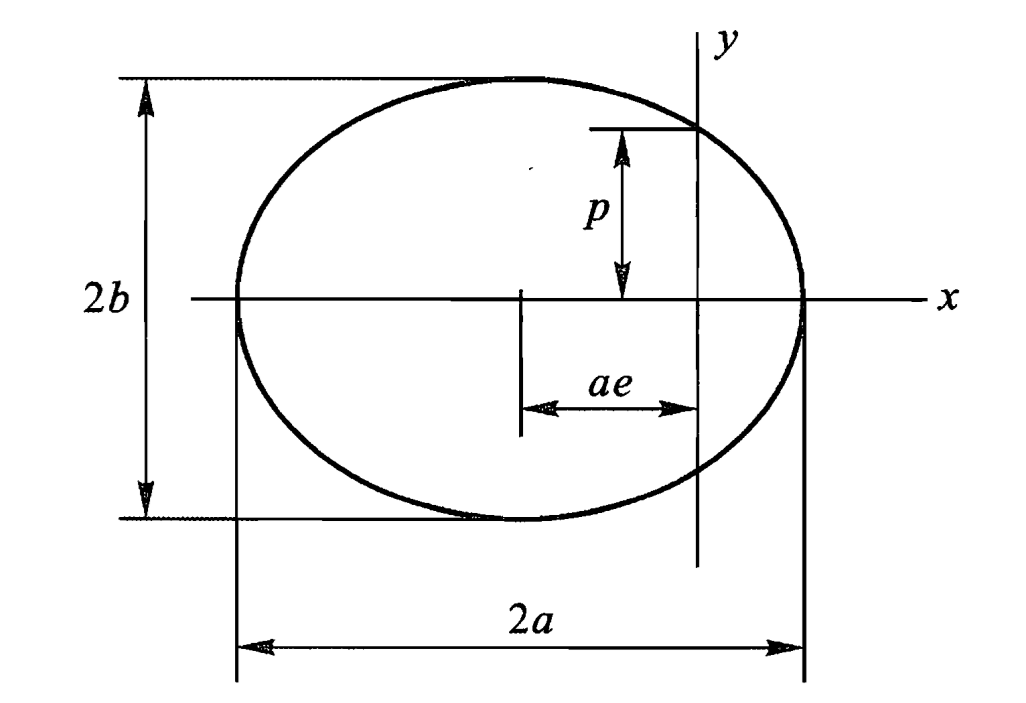
\includegraphics[height=3.5cm ,width=5cm]{CM/kepler1.png}
	\caption{Attractive Kepler orbit with $e < 1$}
\end{figure}
\\
The major and minor semi-axes of the ellipse are
\[a = \frac{p}{1-e^2} = \frac{\alpha}{2|E|} ;\quad b = \frac{p}{\sqrt{1-e^2}} = \frac{M}{\sqrt{2m|E|}}.\]
The least and greatest distances from the centre of the field (the focus of the ellipse) are
\[r_{\mathrm{min}} = \frac{p}{1+e} = a(1-e) ;\quad r_{\mathrm{max}} = \frac{p}{1-e} = a(1+e).\]
The period of revolution in an elliptical orbit is
\[T = \frac{\pi a b}{\frac{1}{2}r^2 \dot{\phi}} = 2\pi a^{3/2}\sqrt{\frac{m}{\alpha}} = \pi \alpha \sqrt{\frac{m}{2|E|^3}}.\]
\\
If $E > 0$, the path is a hyperbola with the origin as internal focus. 
\begin{figure}[!h]
	\centering
	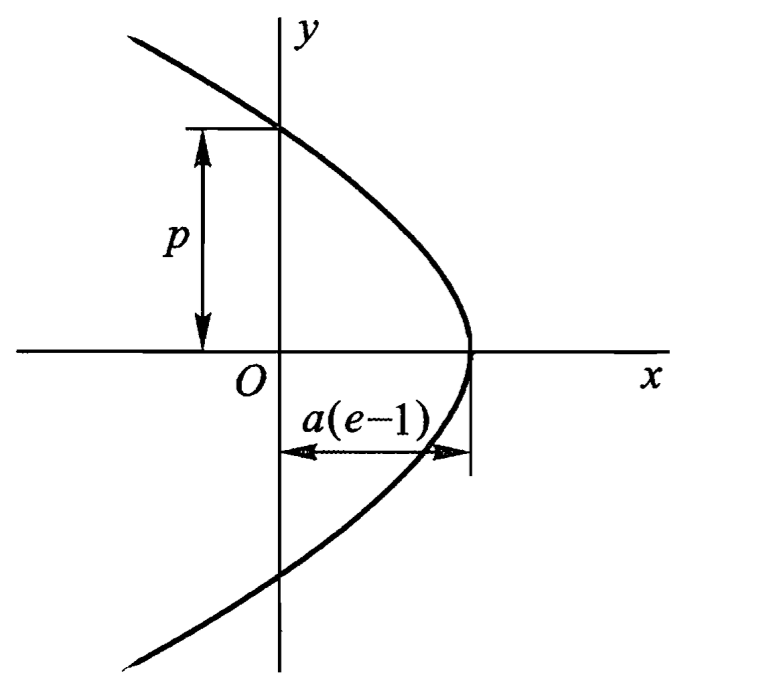
\includegraphics[height=3.5cm ,width=3.8cm]{CM/kepler2.png}
	\caption{Attractive Kepler orbit with $e > 1$}
\end{figure}
The distance of the perihelion from the focus is
\[r_{\mathrm{min}} = \frac{p}{1+e} = a(1-e),\]
where $a = {p}/{(1-e^2)^2} = {\alpha}/{2E}$ is the semiaxis of the hyperbola.
\\ \\
If $E = 0$, the eccentricity $e = 1$, and the particle moves in a parabola with perihelion distance $r_{\mathrm{min}} = {p}/{2}$. This case occurs if the particle starts from rest at infinity.
\\ \\
Let us now consider motion in a repulsive field, where
\[U= \frac{\alpha}{r} \quad (\alpha > 0).\]
Here the effective potential energy is
\[U_{\mathrm{eff}} = \frac{\alpha}{r} + \frac{M^2}{2mr^2} \]
and decreases monotonically from $+\infty$ to zero as $r$ varies from zero to infinity.
The energy of the particle must be positive, and the motion is always infinite. The calculations are exactly similar to those for the attractive field.
The path is a hyperbola:
\[\frac{p}{r} = -1 + e\cos\phi.\]
\begin{figure}[!h]
	\centering
	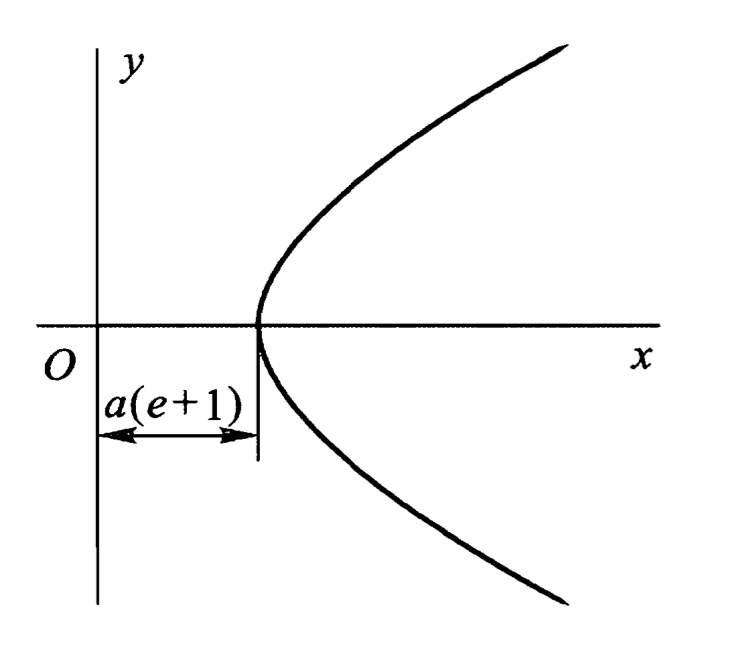
\includegraphics[height=3.3cm ,width=3.7cm]{CM/kepler3.png}
	\caption{Repulsive Kepler orbit}
\end{figure}
\\
The perihelion distance is
\[r_{\mathrm{min}} = \frac{p}{-1+e} = a(1+e).\]
\\
There is an integral of the motion which exists only in fields $U = {\alpha}/{r}$. 
It is easy to verify by direct calculation that the quantity
\[\bm{v}\times\bm{M} + \frac{\alpha \bm{r}}{r} \]
is constant. The direction of the conserved vector is along the major axis from the focus to the perihelion, and its magnitude is $\alpha e$. This is most simply seen by considering its value at perihelion.

\section{Disintegration and collisions of particles}
Let us consider a spontaneous disintegration of a particle into two constituent parts. 
This process is most simply described in a frame of reference in which the particle is at rest before the disintegration.
The law of conservation of momentum shows that the sum of the momenta of the two particles formed in the disintegration is then zero; that is, the particles move apart with equal and
opposite momenta. The magnitude $p_0$ of either momentum is given by the law of conservation of energy:
\[E_i = E_{1i} + \frac{p_0^2}{2m_1} + E_{2i} + \frac{p_0^2}{2m_2}, \]
where $m_1$ and $m_2$ are the masses of the particles, $E_{1i}$ and $E_{2i}$, their internal energies, and $E_{i}$ the internal energy of the original particle. If $\epsilon$ is the disintegration energy, i.e. the difference
\[\epsilon = E_i - E_{1i} - E_{2i} \]
which must obviously be positive, then
\[\epsilon = \frac{p_0^2}{2m}, \]
where $m$ is the reduced mass of the two particles.
\\ \\
Let us now change to a frame of reference in which the primary particle moves with velocity $\bm{V}$ before the break-up.
This frame is usually called the laboratory system, or L system, in contradistinction to the centre-of-mass
system, or C system, in which the total momentum is zero. 
Let us consider one of the resulting particles, and let $\bm{v}$ and $\bm{v}_0$ be its velocities in the L and
the C system-respectively. 
\begin{figure}[!h]
	\centering
	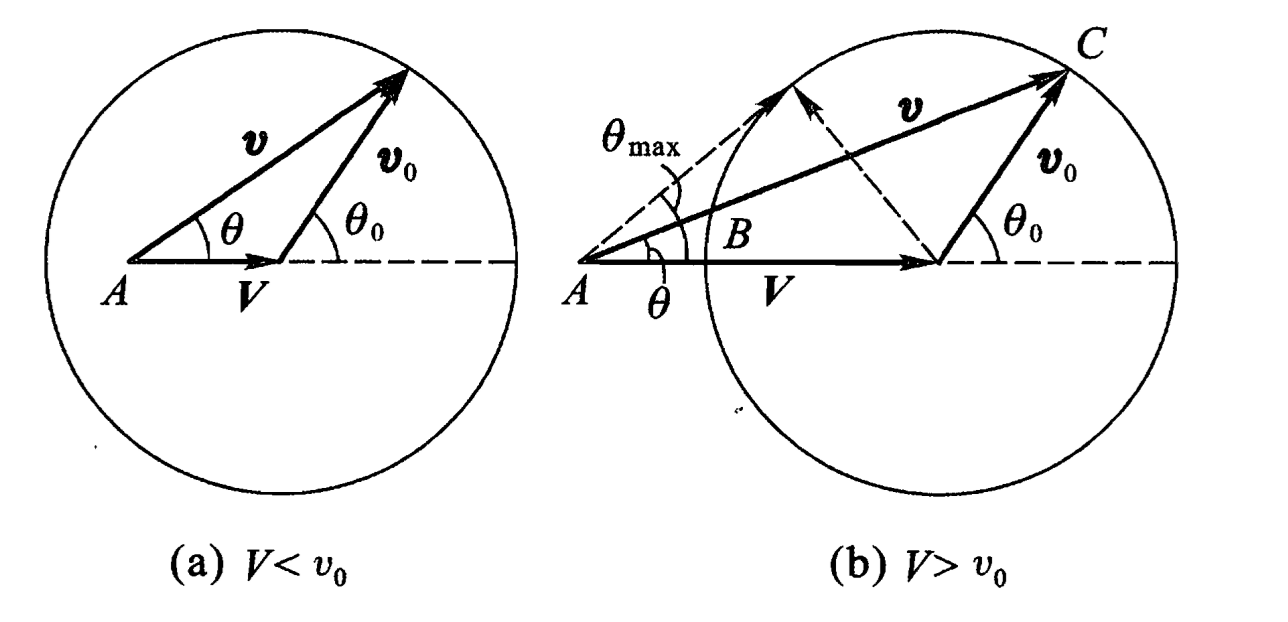
\includegraphics[height=4.5cm ,width=9.5cm]{CM/disintegration.png}
	\caption{Disintegration in L and C frame}
\end{figure}
\noindent
The relation between the angles $\theta$ and $\theta_0$ in the L and C systems is evidently,
\[\tan\theta = \frac{v_0\sin\theta_0}{V+v_0\cos\theta_0}.\]
In physical applications we are usually concerned with the disintegration of not one but many similar particles, and this raises the problem of the distribution of the resulting particles in direction, energy, etc. 
We shall assume that the primary particles are randomly oriented in space, i.e. isotropically on average.
\\ \\
In the C system, every resulting particle has the same energy, and their directions of motion are isotropically distributed. The fraction of particles entering a solid angle element $do$ is $\frac{do}{4\pi}$. 
Thus the distribution with respect to the angle $\theta_0$ is
\[\frac{1}{2}\sin\theta_0 d\theta_0.\]
The corresponding distributions in the L system are obtained by an appropriate transformation. For example, let us work out the kinetic energy distribution in the L system.
Since
\[v^2 = V^2 + v_0^2 + 2Vv_0\cos\theta_0,\] 
we have $d(v^2) = d\cos\theta_0$. Thus the kinetic energy can distributed uniformly over between $T_{\mathrm{min}} = \frac{1}{2}(v_0-V)^2$ and $T_{\mathrm{max}}= \frac{1}{2}m(v_0+V)^2$.
\\ \\
A collision between two particles is said to be elastic if it involves no change in their internal state. The collision is most simply described in the C system.The velocities of the particles before the collision are related to their velocities $\bm{v}_1$ and
$\bm{v}_2$ in the L system by $\bm{v}_{10} = m_2\bm{v}/(m_1+m_2)$, $\bm{v}_{20} = -m_1\bm{v}/(m_1+m_2)$,
where $\bm{v} = \bm{v}_1-\bm{v}_2$.
Because of the law of conservation of momentum, the momenta of the two particles remain equal and opposite after the collision, and are also unchanged in magnitude, by the law of conservation of energy. 
Thus, in the C system the collision simply rotates the velocities, which remain opposite in direction and unchanged in magnitude. The velocities of the two particles after the collision are
\[\bm{v}'_{10} = \frac{m_2v\bm{n}_0}{m_1+m_2}, \quad \bm{v}'_{20} = -\frac{m_1v\bm{n}_0}{m_1+m_2}.\]
The velocities in the L system after the collision are therefore
\[\bm{v}'_{1} = \frac{m_2v\bm{n}_0}{m_1+m_2} + \frac{m_1\bm{v_1}+m_2\bm{v_2}}{m_1+m_2}, \quad \bm{v}'_{2} = -\frac{m_1v\bm{n}_0}{m_1+m_2} + \frac{m_1\bm{v_1}+m_2\bm{v_2}}{m_1+m_2}.\]
Multiplying equations by $m_1$ and $m_2$ respectively, we obtain
\[\bm{p}'_{1} = mv\bm{n}_0 + \frac{m_1(\bm{p}_1 + \bm{p}_2)}{m_1+m_2}, \quad \bm{p}'_{2} = -mv\bm{n}_0 + \frac{m_2(\bm{p}_1 + \bm{p}_2)}{m_1+m_2}.\]
\begin{figure}[!h]
	\centering
	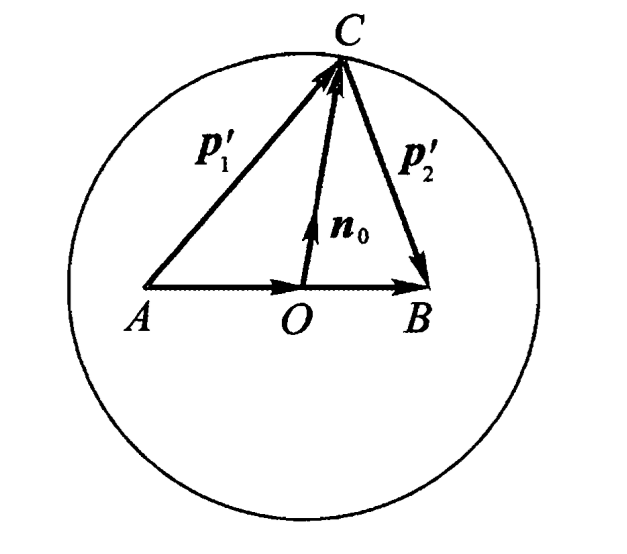
\includegraphics[height=3cm ,width=3.3cm]{CM/collision1.png}
	\caption{Collision in L and C frame}
\end{figure}
\noindent
Let us consider in more detail the case where one of the particles ($m_2$, say) is at rest before the collision. In that case the distance $OB = {m_2p_1}/{(m_1+m_2)} = mv$ is equal to the radius. The vector $\vec{AB}$ is equal to the momentum $\bm{p}_1$ of the particle $m_1$ before the collision.
\begin{figure}[!h]
	\centering
	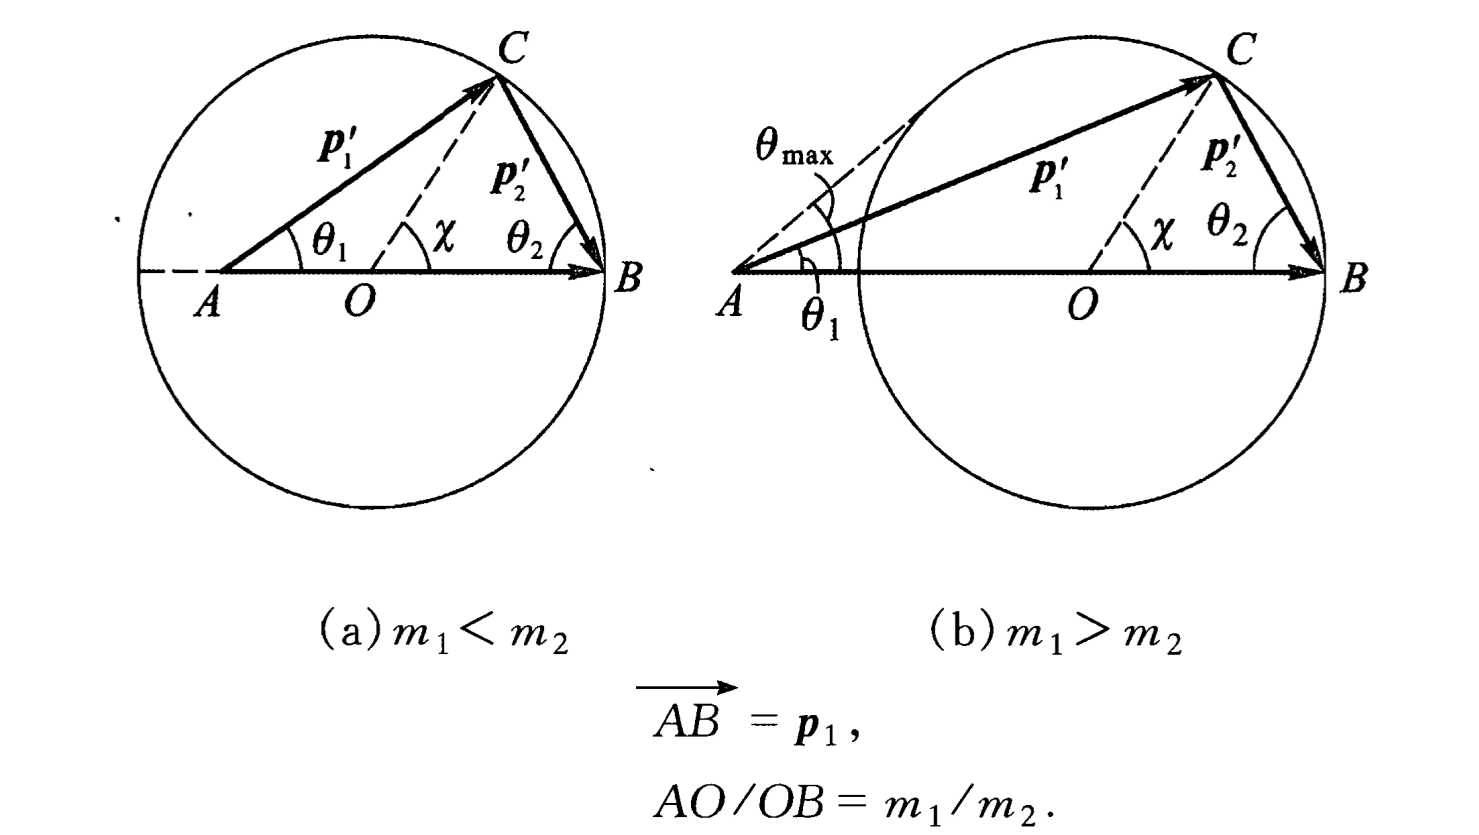
\includegraphics[height=4.2cm ,width=7.5cm]{CM/collision2.png}
	\caption{Collision with 2 at rest}
\end{figure}
\noindent
$\theta_1$ and $\theta_2$ can be expressed in terms of $\chi$ by
\[\tan\theta_1 = \frac{m_2\sin\chi}{m_1 + m_2 \cos\chi} \quad \theta_2 = \frac{1}{2}(\pi - \chi).\]
The magnitudes of the velocities of the two particles after the collision in terms of $\chi$ are
\[v'_1 = \frac{\sqrt{m_1^2 + m_2^2 + 2m_1m_2\cos\chi}}{m_1+m_2}v \quad v'_2 = \frac{2m_1v}{m_1+m_2}\sin\frac{1}{2}\chi.\]
If $m_1 < m_2$, the velocity of $m_1$ after the collision can have any direction.
If $m_1 > m_2$, this particle can be deflected only through an angle not exceeding $\theta_\mathrm{max}$ from its original direction. Evidently
\[\sin\theta_{\mathrm{max}} = \frac{m_2}{m_1}.\]
The collision of two particles of equal mass, of which one is initially at rest, is especially simple. In this case both B and A lie on the circle.
\begin{figure}[!h]
	\centering
	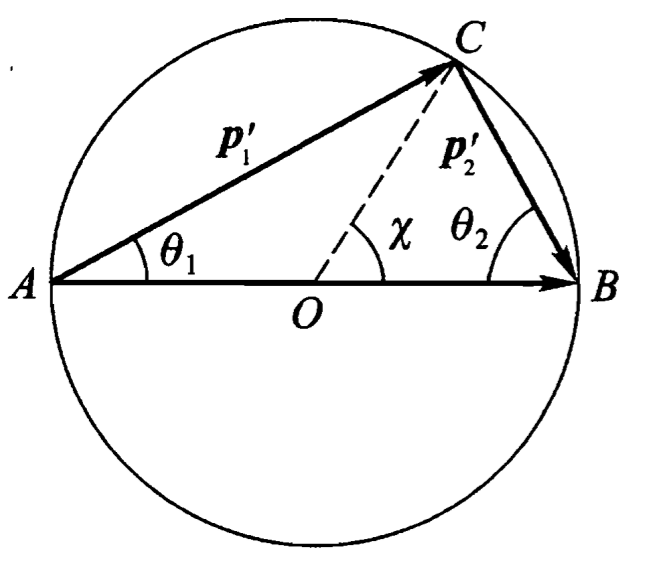
\includegraphics[height=2.9cm ,width=3.25cm]{CM/collision3.png}
	\caption{Collision of equal mass}
\end{figure}
\[\theta_1 = \frac{1}{2}\chi ,\quad \theta_2 = \frac{1}{2}(\pi-\chi);\]
\[v'_1 = v\cos\frac{1}{2}\chi ,\quad v'_2 = v\sin\frac{1}{2}\chi.\]
After the collision the particles move at right angles to each other.

\section{Scattering and cross section}
Scattering is a general physical process where some forms of radiation, such as light, sound, or moving particles, are forced to deviate from a straight trajectory by one or more paths due to localized non-uniformities in the medium through which they pass.  In classical mechanics, scattering generally refer to particle-particle collisions.
The definition of cross section  of a scattering process is
\[\sigma \equiv \frac{\mbox{Number of Events per target}}{\mbox{Time} \times \mbox{Incident Flux}}.\]
Here, the incident flux are measured in the frame of target particle. Recall that when we reduce two body problem in to one body problem, $\bm{r} = \bm{r}_1 - \bm{r}_2$ is the coordinates of projectile in the frame of target. Thus the scattering process can be represented by the reduced mass moving in the central field. 
\begin{figure}[!h]
	\centering
	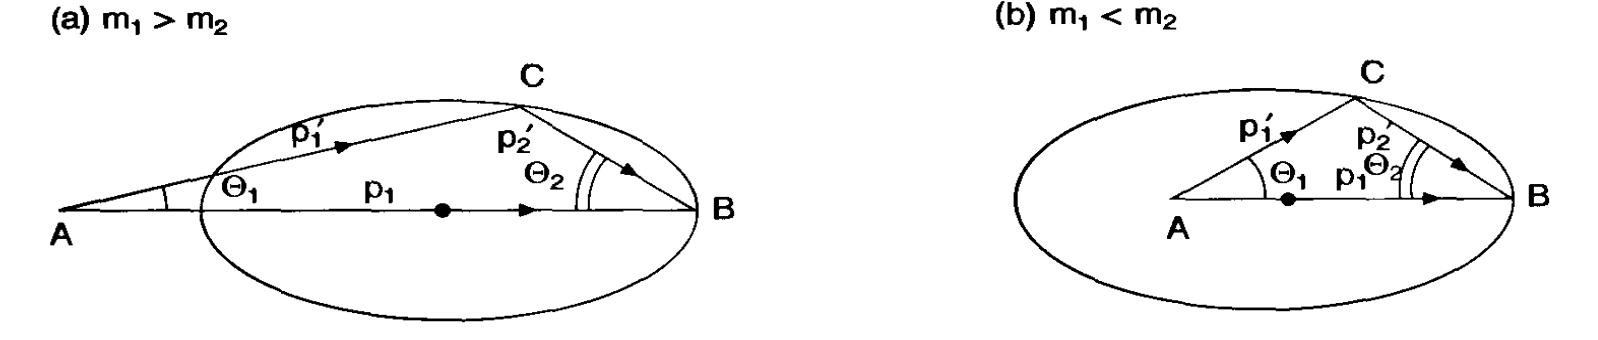
\includegraphics[height=3.9cm ,width=5.2cm]{CM/scattering.png}
	\caption{Scattering in central field}
\end{figure}
\\
And we have
\[\phi_0 = \int_{r_{\mathrm{min}}}^{\infty} \frac{Mdr}{r^2 \sqrt{2m(E-U(r))-\frac{M^2}{r^2}}} ,\quad \chi = |\pi - 2\phi_0|.\]
Since
\[E = \frac{1}{2}m v_{\infty}^2 ,\quad M = m\rho v_{\infty},\]
we can get the relation between  $\chi$ and $\rho$. Suppose the number density of the particles is $n$, then the incident flux is $nv_{\infty}$, number of events that particles are scattered into the solid angle $do = \sin\chi d\chi d\phi$ at $(\chi,\phi)$ in time $T$ is
\[d\rho \rho(\chi) d\phi nv_{\infty} T .\]
Therefore, we have
\[d\sigma = \rho(\chi) d\rho d\phi = \frac{\rho(\chi)}{\sin\chi} \left| \frac{d\rho}{d\chi} \right| do.\]
In C system, we have $\bm{r}_1 = {m_2 \bm{r}}{(m_1+m_2)} $, so the scattering angle of particle 1 is the same as $\chi$. While in L system (particle 2 is at rest before scattering), we must making corresponding transformation to get the right expression for cross section.

\subsubsection{Rutherford's formula}
One of the most important applications of the formulae derived above is to the scattering of charged particles in a Coulomb field. As $U = {\alpha}/{r}$, we have
\[\phi_0 = \arccos \frac{\alpha/mv^2_{\infty}\rho}{\sqrt{1+(\alpha/mv^2_{\infty}\rho)^2}}.\]
Recall that $\chi = (\pi-\phi_0)/2$, we can obtain that
\[\rho^2 = \frac{\alpha^2}{m^2v_{\infty}^4} \cot^2 \frac{1}{2}\chi \]
and
\[d\sigma = \left( \frac{\alpha}{2mv_{\infty}^2} \right)^2 \frac{do}{\sin^4 \frac{1}{2}\chi}.\]
This is Rutherford's formula. It may be noted that the effective cross-section is independent of the sign of $\alpha$, so that the result is equally valid for repulsive and attractive Coulomb fields.
\\ \\
Formula above gives the effective cross-section in the frame of reference in which the centre of mass of the colliding particles is at rest. The transformation to the laboratory system is effected by means of
\[\tan\theta_1 = \frac{m_2\sin\chi}{m_1 + m_2 \cos\chi} ,\quad \theta_2 = \frac{1}{2}(\pi - \chi).\]
For particles initially at rest, we have
\[d\sigma_2 = \left ( \frac{\alpha}{mv^2_{\infty}} \right )^2 \frac{do_2}{\cos^3 \theta_2}.\]
The same transformation for the incident particles leads, in general, to a very complex formula, and we shall merely note two particular cases.
\\ \\
If the mass $m_2$ of the scattering particle is large compared with the mass $m_1$ of the scattered particle, then $\chi = \theta_1$ and $m = m_1$, so that
\[d\sigma_1 = \left ( \frac{\alpha}{4E_1}\right )^2 \frac{do_1}{\sin^4 (\frac{1}{2}\theta_1)} ,\]
where $E_1 = m_1v^2_{\infty}/2$ is the energy of the incident particle.
If the masses of the two particles are equal, then by $\theta_1 = {\chi}/{2}$, we have
\[d\sigma_1 =  \left ( \frac{\alpha}{E_1}\right )^2 \frac{\cos\theta_1}{\sin^4\theta_1} do_1.\]
If the particles are entirely identical, that which was initially at rest cannot be distinguished after the collision. The total effective cross-section for all
particles is obtained by adding $do_1$ and $do_2$, so
\[d\sigma = \left ( \frac{\alpha}{E_1}\right )^2 \left ( \frac{1}{\sin^4\theta} + \frac{1}{\cos^4\theta} \right )\cos\theta do.\]
Let us return to the general formula and use it to determine the distribution of the scattered particles with respect to the energy lost in the collision. 
When the masses of the scattered and scattering particles are arbitrary, the velocity acquired by the latter is given in terms of the angle of scattering in the C system by
\[v'_2 = \frac{2m_1}{m_1+m_2} v_{\infty} \sin \frac{\chi}{2}.\]
The energy acquired by 2 and lost by 1 is therefore
\[\epsilon = \frac{2m^2}{m_2} v_{\infty}^2 \sin^2 \frac{\chi}{2} .\]
Expressing $\sin \frac{\chi}{2}$ in terms of $\epsilon$, we obtain
\[d\sigma = 2\pi \frac{\alpha^2}{m_2 v^2_{\infty}} \frac{d\epsilon}{\epsilon^2}.\]
This is the required formula: it gives the effective cross-section as a function, of the energy loss $\epsilon$, which takes values from zero to $\epsilon_{\mathrm{max}} = 2m^2 v_{\infty}^2 /m_2$.

\chapter{Small Oscillation}
\section{Small oscillation in one dimensional}
Let us consider the motion in one dimension, the potential energy of the particle is $V = V(q)$. If we choose the coordinate of equilibrium point as $q=0$, then $ \frac{\partial V}{\partial q} |_{q=0} = 0$. Expand $V(q)$ around $q=0$, we have
\[V(q) = V(0) + \frac{1}{2}  \frac{\partial^2 V}{\partial q^2} |_{q=0} \; q^2 + \cdots  \]
If the equilibrium point is stable, we have
\[\frac{\partial^2 V}{\partial q^2} |_{q=0} \equiv V''(0) > 0.\]
For small oscillation, we can neglect the higher orders of $q$ and the Lagrangian can be written as
\[L = \frac{1}{2}m\dot{q} - \frac{1}{2}V''(0)q^2.\]
The Euler-Lagrangian equation is
\[\ddot{q} + \omega_0^2 q = 0 ,\quad \omega_0^2 = \frac{V''(0)}{m}.\]
The general solution is
\[q = A\cos(\omega_0 t + \phi).\]
$A$ and $\phi$ depends on the initial condition. 
\\ \\
If there is a damped force which is proportional to the velocity of the particle, then we have
\[\ddot{q} + \frac{1}{Q}\dot{q} + \omega_0^2 q = 0.\]
If $Q > {1}/{2\omega_0}$, we have
\[q = A e^{-\frac{t}{2Q}} \cos(\omega t + \phi) ,\quad \omega = \sqrt{\omega_0^2 - \frac{1}{4Q^2}}.\]
It is called under damped oscillation.
If $Q < {1}/{2\omega_0}$, we have
\[q = Ae^{\lambda_+ t} + B Ae^{\lambda_- t},\]
where
\[\lambda_{\pm} = -\frac{1}{2Q} \pm \sqrt{\frac{1}{4Q^2} - \omega_0^2 }.\]
It is called over damped oscillation.
If $Q = {1}/{2\omega_0}$, we have
\[q = C(1+Dt)e^{-\omega_0 t}.\]
It is called critical damped oscillation.

\section{Forced oscillation}
The equation of motion for forced oscillation is
\[\ddot{q} + \frac{1}{Q}\dot{q} + \omega_0^2 q = F(t).\]
The form of solution is
\[q = q_{\mathrm{s}} + q_{\mathrm{g}} \]
and $q_{\mathrm{g}}$ is the general solution of the homogeneous equation and $q_{\mathrm{s}}$ is an arbitrary special solution of the equation. In order to get $q_{\mathrm{s}}$, we consider the following equation
\[\ddot{G} + \frac{1}{Q}\dot{G} + \omega_0^2 G = \delta(t-t') \]
and its solution is $G(t,t')$.
Then we have
\[q_{\mathrm{s}} = \int_{-\infty}^{\infty} F(t')G(t-t')dt'.\]
For under damped oscillation, we have
\[G(t,t') = \begin{cases} \frac{e^{-\frac{t-t'}{2Q}}}{\omega} \sin\omega(t-t') ,\quad t>t'\\ 0 ,\quad t<t'\end{cases} \]
and so
\[q_{\mathrm{s}} = \int_{0}^{\infty} F(t-t') \frac{e^{-\frac{t'}{2Q}}}{\omega} \sin\omega t' dt'.\]
A special case is that
\[F(t) = F_0 \cos\Omega t ,\]
and we have
\[q(t) = \frac{F_0}{\sqrt{(\Omega^2 - \omega_0^2 + \frac{1}{2Q^2})^2 + \frac{\omega^2}{Q^2}}} \cos(\Omega t + \phi), \]
where
\[\tan \phi = \frac{\frac{\Omega}{Q}}{\omega_0^2 - \Omega^2}.\]
When
\[\Omega = \sqrt{\omega_0^2 - \frac{1}{2Q^2}},\]
we have
\[q_{\mathrm{max}} = \frac{QF_0}{\omega}.\]
It is called resonance. 

\section{Non-linear oscillation and perturbation theory}
Consider the equation of motion
\[\ddot{q} + \omega_0^2 q + \epsilon q^3 = 0.\]
Suppose $\epsilon$ is very small, then we can expand
\[q = q_0 + \epsilon q_1 + \epsilon^2 q_2 + \cdots \]
and
\[\omega = \omega_0 + \epsilon \omega_1 + \epsilon^2 \omega_2 + \cdots \]
The equation of motion can be written as
\[\ddot{q} + \omega^2 q = (\omega^2 -\omega_0^2)q - \epsilon q^3.\]
Let $\tau \equiv \omega t$ and $q' \equiv {dq}/{d\tau} = {\dot{q}}/{\omega}$, we have
\[q'' + q = (1- \frac{\omega_0^2}{\omega^2})q - \frac{\epsilon}{\omega^2} q^3 = 0.\]
We can solve the equation above power by power and get
\[q_0'' + q_0 = 0 ,\]
\[q_1'' + q_1 = -\frac{q_0^3}{\omega_0^2} + \frac{2\omega_1}{\omega_0}q_0, \]
and so on. 
When doing the perturbation, we must adjust the $\omega_i$ to avoid the resonance solution. The details will be neglect here.
\\ \\
Now let us consider the non-linear oscillation with drive force. The equation of motion is
\[\ddot{q} + \frac{1}{Q}\dot{q} + \omega_0^2 q + \epsilon q^3 = F_0 \cos \omega t.\]
It can be rewritten as
\[\ddot{q} + \omega^2 q = - \frac{1}{Q} \dot{q} + (\omega^2 - \omega_0^2)q - \epsilon q^3 + F_0\cos\omega t.\]
We treat the right hand of the equation as perturbation, so we multiply it by a parameter $\mu$ and let it be $1$ later,
\[\ddot{q} + \omega^2 q = \mu \left (- \frac{1}{Q} \dot{q} + (\omega^2 - \omega_0^2)q - \epsilon q^3 + F_0\cos\omega t \right ).\]
Concerning on the phase lagging effect, we redefine the ``time'' as 
\[\tau \equiv \omega t - \delta, \]
so 
\[q'' + q = \mu \left [ -\frac{1}{Q\omega} q' + \left ( 1- \frac{\omega_0^2}{\omega^2} \right ) q - \frac{\epsilon}{\omega^2} q^3 + \frac{F_0}{\omega^2} \cos (\tau + \delta) \right ].\]
The expansion series of $q$ and $\delta$ are
\[q = q_0 + \mu q_1 + \mu^2 q_2 + \cdots \]
\[\delta = \delta_0 + \mu \delta_1 + \mu^2 \delta_2 + \cdots \]
We can solve the equation above power by power and get
\[q''_0 + q_0 = 0,\]
\[q''_1 + q_1 =  -\frac{1}{Q\omega} q_0' + \left ( 1- \frac{\omega_0^2}{\omega^2} \right ) q_0 - \frac{\epsilon}{\omega^2} q_0^3 + \frac{F_0}{\omega^2} \cos (\tau + \delta_0), \]
and so on. 
The solution of the zeroth order perturbation is
\[q_0 = A_0 \cos\tau.\]
Substitute it into the first order equation, we have
\[q''_1 + q_1 = \left ( \frac{A_0}{Q\omega} - \frac{F_0}{\omega^2} \sin\delta_0 \right ) \sin\tau + \left [ \left ( 1 - \frac{\omega_0^2}{\omega^2}\right ) A_0 - \frac{3\epsilon A_0^3}{4\omega^2} + \frac{F_0}{\omega^2}\cos\delta_0 \right ] \cos\tau - \frac{\epsilon A_0^3}{4\omega^2} \cos 3\tau.\]
To avoid non-physical solution, we have
\[\sin\delta_0 = \frac{A_0 \omega}{F_0 Q} \]
and
\[\left ( 1 - \frac{\omega_0^2}{\omega^2}\right ) A_0 - \frac{3\epsilon A_0^3}{4\omega^2} + \frac{F_0}{\omega^2}\cos\delta_0 = 0.\]
Now, we can get
\[A_0 = \frac{F_0}{\sqrt{\left[ (\omega^2 -\omega_0^2) - \frac{3}{4}\epsilon A_0^2 \right ]^2 + \frac{\omega^2}{Q^2} }}.\]
If we define
\[x \equiv \frac{\omega}{\omega_0} ,\quad y \equiv \frac{A_0 \omega_0^2}{F_0},\]
the equation above can be written as
\[y^2 = \frac{1}{(x^2-1-ay^2)^2 + bx^2}, \]
where
\[a = \frac{3\epsilon F_0^2}{4\omega_0^6}, \quad b = \frac{1}{\omega_0^2 Q^2}.\]
We than can solve for $x$ in terms of $y$,
\[x^2 = \frac{2 + 2ay-b \pm \sqrt{(b-2-2ay)^2-4(a^2y^2+2ay+1-\frac{1}{y})}}{2}.\]
\begin{figure}[!h]
	\centering
	\includegraphics[height=6cm ,width=12cm]{CM/resonance.png}
	\caption{Resonance curve}
\end{figure}
\\ 
Thus the resonance curve has two branches, corresponding to the two roots of the equation above. When the frequency of the drive force increase from left, the amplitude of oscillation will become larger and larger. But when it comes to the point of inflection, the amplitude will drop to the low-right part of the curve. When the frequency of the drive force decrease from right, the amplitude of oscillation will also become larger and larger. When it comes to the point of inflection, the amplitude will jump to the hight-left part of the curve. 
This effect is called hysteresis.

\section{Oscillations of systems with more than one degree of freedom}
Let's look at a system with many degrees of freedom; we have
\[L={\frac {1}{2}}\sum _{i,j}T_{ij}{\dot {q}}_{i}{\dot {q}}_{j}-V\left(q_{1},\ldots q_{n}\right).\]
Let $q_{0,i}$ be an equilibrium position and expand about this point $q_{i}=q_{0,i}+\eta _{i}$, so $\dot{q}_{i}=\dot {\eta }_{i}$.
We can expand the potential energy to give
\[V\left(q_{1},\ldots q_{n}\right)=V\left(q_{0,1},\ldots q_{0,n}\right)+\sum _{i}\left({\frac {\partial V}{\partial q_{i}}}\right)_{q_{0,i}}\eta _{i}+{\frac {1}{2}}\sum _{i,j}\left({\frac {\partial ^{2}V}{\partial q_{i}\partial q_{j}}}\right)_{q_{0,i}}\eta _{i}\eta _{j}+\cdots \]
The first term is a constant with respect to $\eta_i$ and constant terms do not affect the motion. The second term is zero, because $q_{0,i}$ is a point of equilibrium so we are left with
\[L={\frac {1}{2}}\sum _{i,j}\left(T_{ij}{\dot {\eta }}_{i}{\dot {\eta }}_{j}-V_{ij}\eta _{i}\eta _{j}\right), \]
where
\[T_{ij}=T_{ij}\left(q_{0,1},\ldots q_{0,n}\right) ,\quad V_{ij}=\left({\frac {\partial ^{2}V}{\partial q_{i}\partial q_{j}}}\right)_{q_{0,i}},\]
yielding the equations of motion
\[\sum _{j}\left(T_{ij}{\ddot {\eta }}_{j} + V_{ij}\eta _{j}\right)=0.\]
This is a linear differential equation with constant coefficients. We can try the solution
\[\eta _{i}=Ca_{i}e^{-i\omega t}.\]
Thus we have
\[\sum _{j}\left(V_{ij}a_{j}-\omega ^{2}T_{ij}a_{j}\right)=0.\]
This is a matrix equation such that
\[{\vec {\vec {A}}}\cdot {\vec {a}}=0 \]
with
\[{\vec {a}}=\left[{\begin{matrix}a_{1}\\a_{2}\\\vdots \\a_{j}\end{matrix}}\right] \]
and
\[{\vec {\vec {A}}}=\left[{\begin{matrix}V_{11}-\omega ^{2}T_{11}&V_{12}-\omega ^{2}T_{12}&\cdots \\V_{21}-\omega ^{2}T_{21}&V_{22}-\omega ^{2}T_{22}&\cdots \\\vdots &&\end{matrix}}\right].\]
This equation only has a solution is $\det {\vec {\vec {A}}}=0$. This gives a $n$th-degree polynomial to solve for $\omega^2$. We will get $n$ solutions for $\omega^2$ that we can substitute into the matrix equation and solve for $a_j$.

\chapter{Motion of a Rigid Body}
\section{Angular velocity}
Suppose there are two coordinate frames. The frame 2 is rotating with respect to frame 1. If the coordinates of a particle in frame 2 are $r_2=(x_2,y_2,z_2)$.
Then the coordinates of the particle in frame 1 are
\[r_1 = O(t)r_2 ,\]
and we have
\[O^TO=I.\]
Note that
\[\Omega + \Omega^T= 0 ,\quad \Omega \equiv O^T\frac{dO}{dt}.\]
It is easy to derive that
\[\frac{dr_1}{dt} = \frac{dO}{dt}r_2 + O\frac{dr_2}{dt} = OO^T \frac{dO}{dt}r_2 + Ov_2  = O (\Omega r_2 + v_2) ,\quad v_2 \equiv \frac{dr_2}{dt}.\]
Suppose
\[\Omega = \left[ \begin{matrix} 0& -\omega_{2z}& \omega_{2y}\\ \omega_{2z}& 0& -\omega_{2x}\\ -\omega_{2y}& \omega_{2x}& 0\end{matrix} \right] .\]
We can get
\[v_1 \equiv \frac{dr_1}{dt}  = O(\omega_2 \times r_2 + v_2) .\]
Now, we define
\[\omega_1 \equiv O\omega_2.\]
We can verify that
\[O \Omega O^T = \left[ \begin{matrix} 0& -\omega_{1z}& \omega_{1y}\\ \omega_{1z}& 0& -\omega_{1x}\\ -\omega_{1y}& \omega_{1x}& 0\end{matrix} \right] .\]
Therefore, we have
\[v_1 = \omega_1 \times r_1 + Ov_2 ,\]
where $\omega$ is the so-called angular velocity.
\begin{note}
$\omega_1$ is independent of the base vector we choose for frame 2.
If we choose frame 1 differently, $\omega_1$ will transform like an vector.
\end{note}

\section{Dynamics of rigid body}
\subsubsection{Inertial tensor of rigid body}
Suppose there is frame attached to the rigid body, then the coordinate of all the mass point of the rigid body is constant in this frame, i.e.
\[r_1 = r_0(t) + O(t)r_2 ,\quad r_2 \mbox{ is a constant}.\]
Thus we have
\[v_1 = V + \omega_1 \times r_1 = V + O(\omega_2 \times r_2).\]
The kinetic energy of the rigid body is
\[T = \sum \frac{m}{2} (\bm{V} + \bm{\omega} \times \bm{r})^2 = \sum \frac{m}{2} V^2 + \sum m\bm{V}\cdot(\bm{\omega}\times\bm{r}) + \sum \frac{m}{2} (\bm{\omega} \times \bm{r})^2.\]
If we choose the origin of the frame 2 to be the center of mass of the rigid body, we have
\[T = \frac{\mu V^2}{2} + \frac{1}{2}\sum m [\omega^2r^2-(\bm{\omega} \cdot \bm{r})^2].\]
If we define the inertial tensor as
\[I_{ik} = \sum m (x_l^2 \delta_{ik} - x_i x_k),\]
the kinetic energy of the rigid body can be rewritten as
\[T = \frac{\mu V^2}{2} + \frac{1}{2} I_{ik}\omega_i \omega_k ,\]
and the Lagrangian of the rigid body is
\[L = \frac{\mu V^2}{2} + \frac{1}{2} I_{ik}\omega_i \omega_k -U.\]
If the body is regarded as continuous, the sum becomes an integral over the volume of the body:
\[I_{ik} = \int \rho (x_l^2 \delta_{ik} - x_i x_k) dV.\]
Like any symmetrical tensor of rank two, the inertia tensor can be reduced to diagonal form by an appropriate choice of the directions of the axes $x_1$, $x_2$ $x_3$. 
These directions are called the principal axes of inertia, and the corresponding values of the diagonal components of the tensor are called the principal moments of inertia; we shall denote them by $I_1$, $I_2$, $I_3$. 
When the axes $x_1$, $x_2$ $x_3$ are so chosen, the kinetic energy of rotation takes the very simple form
\[T_{\rm rot} = \frac{1}{2} (I_1 \omega_1^2 + I_2 \omega_2^2 + I_3 \omega_3^2).\]
\\ \\
A body whose three principal moments of inertia are all different is called an asymmetrical top. 
If two are equal ($I_1 = I_2 \neq I_3$), we have a symmetrical top. 
In this case the direction of one of the principal axes in the $x_1x_2$-plane may be chosen arbitrarily.
If all three principal moments of inertia are equal, the body is called a spherical top, and the three axes of inertia may be chosen arbitrarily as any three mutually perpendicular axes.
\\ \\
The determination of the principal axes of inertia is much simplified if the body is symmetrical, for it is clear that the position of the centre of mass and the directions of the principal axes must have the same symmetry as the body.
For example, if the body has a plane of symmetry, the centre of mass must lie in that plane, which also contains two of the principal axes of inertia, while the third is perpendicular to the plane.
If a body has an axis of symmetry of any order, the centre of mass must lie on that axis, which is also one of the principal axes of inertia, while the other two are perpendicular to it.
If the axis is of order higher than the second, the body is a symmetrical top. For any principal axis perpendicular to the axis of symmetry can be turned through an angle different from $\pi$ about the latter, i.e. the choice of the perpendicular axes is not unique, and this can happen only if the body is a symmetrical top.
\\ \\
Finally, we may note one further result concerning the calculation of the inertia tensor. 
Although this tensor has been defined with respect to a system of co-ordinates whose origin is at the centre of mass , it may sometimes be more conveniently found by first calculating a similar tensor,
\[I'_{ik} = \sum m (x_l^{'2} \delta_{ik} - x'_i x'_k), \]
defined with respect to some other origin $O'$. 
If the distance $OO'$ is represented by a vector $\bm{a}$, then $\bm{r} = \bm{r'} + \bm{a}$; since, by the definition
of $O$, $\sum m\bm{r} = 0$, we have
\[I'_{ik} = I_{ik} + \mu (a^2\delta_{ik}-a_i a_k).\]
Using this formula, we can easily figure out $I_{ik}$ if $I'_{ik}$ is known.

\subsubsection{Angular momentum}
The value of the angular momentum of systems depends on the point with respect to which it is defined. In the mechanics of a rigid body, the most appropriate point to choose for this purpose is the origin of the moving system of co-ordinates, i.e. the centre of mass of the body. Then we have
\[\bm{M} = \sum m\bm{r} \times (\bm{\omega} \times \bm{r} + \bm{V}) = \sum m \left [ r^2\bm{\omega} - (\omega \cdot \bm{r})\bm{r} \right ],\]
or, in tensor notation,
\[M_i = I_{ik}\omega_k.\]
If the axes $x_1$, $x_2$ $x_3$ are the same as the principal axes of inertia, we have
\[M_1 = I_1 \omega_1 ,\quad M_2 = I_2 \omega_2 ,\quad M_3 = I_3 \omega_3.\]

\subsubsection{Equation of motion}
Since a rigid body has, in general, six degrees of freedom, the general equations of motion must be six in number. They can be put in a form which gives the time derivatives of two vectors, the momentum and the angular momentum of the body.
The first equation is obtained by simply summing the equations $\dot{\bm{p}} = \bm{f}$ for each particle in the body. In terms of the total momentum of the body
\[\bm{P} = \sum \bm{p} = \mu\bm{V}, \]
and total force acting on it $\bm{F} = \sum \bm{f}$, we have
\[\frac{d\bm{P}}{dt} = \bm{F} .\]
Although $\bm{F}$ has been defined as the sum of all the forces $\bm{f}$ acting on the various particles, including the forces due to other particles, $\bm{F}$ actually includes only external forces: the forces of interaction between the particles composing the body must cancel out, since if there are no external forces the momentum of the body, like that of any closed system, must be conserved, i.e. we must have $\bm{F} = 0$. 
\\ \\
Let us now derive the second equation of motion, which gives the time derivative of the angular momentum $\bm{M}$.
To simplify the derivation, it is convenient to choose the fixed (inertial) frame of reference in such a way that the centre of mass is at rest in that frame at the instant considered. We have
\[\dot{\bm{M}} = \frac{d}{dt} \sum \bm{r} \times \bm{p} = \sum \bm{\dot{r}} \times \bm{p} + \sum \bm{r} \times \dot{\bm{p}}.\]
Our choice of the frame of reference (with $\bm{V} = 0$) means that the vectors $\dot{\bm{r}}$ and $\bm{p} = m\bm{v}$ are parallel, so $\dot{\bm{r}} \times \bm{p} = 0$. We have
\[\frac{d\bm{M}}{dt} = \bm{K}, \]
where
\[\bm{K} = \sum \bm{r} \times \bm{f}.\]
Since $\bm{M}$ has been defined as the angular momentum about the centre of mass, it is unchanged when we go from one inertial frame to another. We can therefore deduce that the equation of motion, though derived for a particular frame of reference, is valid in any other inertial frame, by Galileo's relativity principle.
The vector $\bm{r}\times \bm{f}$ is called the moment of the force $\bm{f}$, and so $\bm{K}$ is the total torque, i.e. the sum of the moments of all the forces acting on the body. Like the total force, $\sum \bm{r} \times \bm{f}$ need include only the external forces: by the law of conservation of angular momentum, the sum of the moments of the internal forces in a closed system must be zero.

\subsubsection{Euler's equations}
Let ${d\bm{A}}/{dt}$ be the rate of change of any vector $\bm{A}$ with respect to the fixed system of co-ordinates. We have
\[\frac{d\bm{A}}{dt} = \frac{d'\bm{A}}{dt} + \bm{\omega} \times \bm{A}, \]
where
${d'\bm{A}}/{dt}$ is the rate of change of the $\bm{A}$'s components in the body system of coordinates. Therefore, we have
\[\frac{d'\bm{M}}{dt} + \bm{\omega} \times \bm{M} = \bm{K}.\]
Suppose the principal axes of inertia are $x_1$, $x_2$ $x_3$, so we have
\begin{eqnarray}
I_1 \frac{d\omega_1}{dt} + (I_3-I_2)\omega_2\omega_3 &=& K_1 ;\nonumber \\
I_2 \frac{d\omega_2}{dt} + (I_1-I_3)\omega_1\omega_3 &=& K_2 ;\nonumber \\
I_3 \frac{d\omega_1}{dt} + (I_2-I_1)\omega_1\omega_2 &=& K_3 .\nonumber
\end{eqnarray}
These are called Euler's equations.

\section{Eulerian angle}
The motion of a rigid body can be described by means of the three co-ordinates of its centre of mass and any three angles which determine the orientation of the axes $x_1$, $x_2$ $x_3$ in the moving system of coordinates relative to the fixed system $X$, $Y$, $Z$. These angles may often be conveniently taken as what are called Eulerian angles.
\begin{figure}[!h]
	\centering
	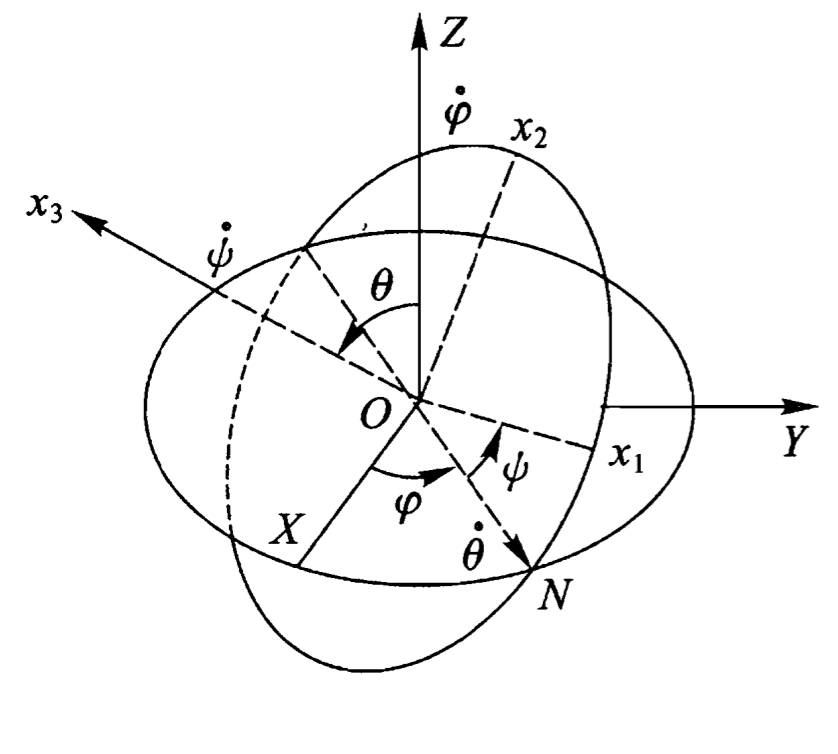
\includegraphics[height=5.7cm ,width=6.3cm]{CM/euler.png}
	\caption{Eulerian angle}
\end{figure}
The moving $x_1x_2$-plane intersects the fixed $XY$-plane in some line $ON$, called the line of nodes. 
This line is evidently perpendicular to both the $Z$-axis and the $x_3$-axis; we take its positive direction as that of the vector product $\bm{z} \times \bm{x}_3$.
We take, as the quantities defining the position of the axes $x_1$, $x_2$ $x_3$ relative to the axes $X$, $Y$, $Z$ the angle $\theta$ between the $Z$ and $x_3$ axes, the angle $\phi$ between the $X$-axis and $ON$, and the angle $\psi$  between the $x_1$ and $ON$.
\\ \\
Let us now express the components of the angular velocity  vector $\omega$ along the moving axes $x_1$, $x_2$ $x_3$ in terms of the Eulerian angles and their derivatives. 
To do this, we must find the components along those axes of the angular velocities $\dot{\theta}$, $\dot{\phi}$, $\dot{\psi}$. The angular velocity $\dot{\theta}$ is along the line of nodes $ON$. The angular velocity $\dot{\phi}$ is along the $Z$-axis. The angular velocity $\psi$ is along the $x_3$-axis. Collecting the components along each axis, we have
\begin{eqnarray}
\omega_1 &=& \dot{\phi}\sin\theta\sin\psi + \dot{\theta}\cos\psi; \nonumber \\
\omega_2 &=& \dot{\phi}\sin\theta\cos\psi - \dot{\theta}\sin\psi; \nonumber \\
\omega_3 &=& \dot{\phi} \cos\theta + \dot{\psi}. \nonumber
\end{eqnarray}
For a symmetrical top, by using the fact that the choice of directions of the principal axes $x_1$, $x_2$ is arbitrary for a symmetrical top. 
If the $x_1$ axis is taken along the line of nodes $ON$, i.e. $\psi = 0$, the components of the angular velocity are simply
\[\omega_1 = \dot{\theta} ,\quad \omega_2 = \dot{\phi}\sin\theta ,\quad \omega_3 = \dot{\phi}\cos\theta + \dot{\psi}.\]
For the free motion of a symmetrical top, we take the $Z$-axis of the fixed system of coordinates in the direction of the constant angular momentum $M$ of the top. The $x_3$-axis of the moving system is along the axis of the top; let the $x_1$-axis coincide with the line of nodes at the instant considered. 
Then the components of the vector $M$ are
\[M_1 = I_1\dot{\theta} ,\quad M_2 = I_2 \dot{\phi}\sin\theta ,\quad M_3 = I_3(\dot{\phi}\cos\theta + \dot{\psi}).\]
Since the $x_1$-axis is perpendicular to the $Z$-axis, we have
\[M_1 = 0 ,\quad M_2 = M\sin\theta ,\quad M_3 = M\cos\theta.\]
Comparison gives
\[\dot{\theta} = 0 ,\quad  \dot{\phi} = \frac{M}{I_1} ,\quad \dot{\phi}\cos\theta + \dot{\psi} = \frac{M\cos\theta}{I_3}.\]
The first of these equations gives $\theta = \mbox{ constant} $, i.e. the angle between the axis of the top and the direction of $\bm{M}$ is constant. The second equation gives
the angular velocity of precession $\dot{\phi} = {M}/{I_1}$. Finally, the third equation gives the angular velocity with which the top rotates about its own axis $\omega_3 = {M\cos\theta}/{I_3}$.
\part{Classical Field Theory}
\chapter{Special Relativity}
\section{The principle of relativity}
First, we assume there is an upper limit $c$ for the velocity of propagation of interaction. Second, we assume that all inertial reference frames are the same in describing the law of physics. Then, we can find the invariant intervals when transforming from one inertial reference frame to another, $ds^2 = -c^2 dt^2 + dx^2 + dy^2 + dz^2$. 
(In the following, we adopt the unit system in which $c$ equals $1$.) The transformation between different inertial frame preserving the intervals is called Lorentz transformation, which can be written as
\[\overline{x}^{\mu} = \Lambda^{\mu}_{\phantom{\mu}\nu} x^{\nu}.\]
The invariant symbol of the vector representation of Lorentz transformation is $\eta^{\mu \nu}$,
\[\Lambda^{\mu}_{\phantom{\mu}\rho}  \Lambda^{\nu}_{\phantom{\nu}\sigma}  \eta^{\rho \sigma} = \eta^{\mu \nu},\]
where,
\[\eta^{\mu \nu} \equiv \left[ 
\begin{matrix} 
-1& & & \\ 
& +1 & & \\
& & +1 & \\
& & & +1
\end{matrix} 
\right].\]
The inverse matrix of $\eta^{\mu \nu}$ is
\[\eta_{\mu \nu} = \left[ 
\begin{matrix} 
-1& & & \\ 
& +1 & & \\
& & +1 & \\
& & & +1
\end{matrix} 
\right].\]
We can use $\eta^{\mu \nu}$ and and its inverse $\eta_{\mu \nu}$ to raise and lower vector indices, 
\[x_{\mu} \equiv \eta_{\mu \nu} x^{\nu}.\]
And we can verify the following identities,
\[\Lambda^{\mu}_{\phantom{\rho}\rho} \Lambda_{\nu}^{\phantom{\rho}\rho} = \delta^{\mu}_{\nu};\]
\[x^{\mu} = \eta^{\mu \nu} x_{\nu};\]
\[\overline{x}_{\mu} = \Lambda_{\mu}^{\phantom{\mu}\nu} x_{\nu};\]
\[\Lambda_{\mu}^{\phantom{\mu}\rho} \Lambda_{\nu} ^{\phantom{\nu}\sigma}  \eta_{\rho \sigma} = \eta_{\mu \nu}.\]
In a special case where the new reference frame moves along $\hat{1}$ direction with velocity $\beta$, we have
\[\overline{x}^{0} = \gamma x^0 - \gamma \beta x^1,\]
\[\overline{x}^{1} = -\gamma \beta x^0 + \gamma x^1,\]
where $\gamma \equiv (1-\beta^2)^{-1/2}$.
\\ \\
Some physical quantities will behave like a tensor (vector, scalar) when transforming form one inertial frame to another. For example,
\paragraph{scalar} proper time $d \tau$, mass $m$, electrical charge $e$.
\paragraph{vector} four velocity $u^{\mu} \equiv {dx^{\mu}}/{d \tau}$, four momentum $p^{\mu} \equiv m u^{\mu}$, four acceleration $a^{\mu} \equiv {du^{\mu}}/{d \tau}$, four force $f^{\mu} \equiv m a^{\mu}$.
\\ \\
We can also define the corresponding three vector.
\paragraph{three velocity} $\hat{v}^{i} \equiv {dx^i}/{dt}$.
\[u^0 = \gamma, u^i = \gamma \hat{v}^i.\]
If the new reference frame move along $\hat{1}$ direction with velocity $\beta$, we have
\[\overline{\hat{v}}^1 = \frac{\hat{v}^1 - \beta}{1-\hat{v}^1 \beta};\]
\[\overline{\hat{v}}^2 = \frac{\hat{v}^2}{\gamma(1-\hat{v}^2 \beta)};\]
\[\overline{\hat{v}}^3 = \frac{\hat{v}^3}{\gamma(1-\hat{v}^3 \beta)}.\]
\paragraph{three momentum} $\hat{p}^{i} \equiv p^i$
\paragraph{three acceleration} $\hat{a}^{i} \equiv {dv^i}/{dt}$
\paragraph{three force} $\hat{f}^i \equiv {d\hat{p}^i}/{dt}$
\[f^i = \gamma \hat{f}^i.\]

\section{Relativistic Mechanics}
For a free particle, we have following equations of motion:
\[\frac{dp^{\mu}}{d\tau} = 0.\]
It can be formulated in several ways
\subsubsection{Lagrangian formulation}
\[S=-m\int_{a}^{b} d\tau, \ \ \ \ \delta x^{\mu}(a) = \delta x^{\mu}(b) = 0.\]
\[\delta S = 0 \Rightarrow m\frac{du^{\mu}}{d\tau} = 0.\]
\subsubsection{Hamiltonian formulation}
\[S = \int_{t_1}^{t_2} L dt , \quad L = - m \sqrt{1-\dot{x}_i\dot{x}^i}.\]
\[\pi^i = \frac{\partial L}{\partial \dot{x}_i} = \gamma m \eta^{ij}\dot{x}_j.\]
\[H = \pi^i \dot{x}_i - L = \gamma m = \sqrt{m^2 + \pi^i \pi_i}.\]
Therefore, the Hamiltonian equations are
\[\dot{\pi}^i = 0, \ \ \ \ \dot{x_i} = \eta_{ij}\frac{\pi^j}{\sqrt{m^2 + \pi^k \pi_k}}.\]
\subsubsection{Hamiltonian-Jacobi equation}
\[H = -\frac{\partial S}{\partial t}, \ \ \ \ \pi^i = \frac{\partial S}{\partial x_i}.\]
Note that $p^0 = H$, $p^i = \pi^i$, we have $p^{\mu} = \partial^{\mu} S$. The Hamiltonian-Jacobi equation can be written as
\[\left(\frac{\partial S}{\partial t}\right)^2 = m^2 + \left(\frac{\partial S}{\partial x}\right)^2 + \left(\frac{\partial S}{\partial y}\right)^2 + \left(\frac{\partial S}{\partial z}\right)^2.\]
\\ \\
For a non-free particle, we have the revised newton's second law:
\[f^{\mu} = \frac{dp^{\mu}}{d\tau}.\]
The formula is the definition of the four force. It can also be written in three vector as
\[\hat{f}^i = \gamma m \hat{a}^i + \gamma^3 (\hat{a}^j \hat{v}_j) m \hat{v}^i.\]
\\ \\
If the system consists of more than one particles interacting with each other. We have the conservation laws from the symmetry.
\subsubsection{Translational symmetry and conservation of momentum}
\[\overline{x}^{\mu} = x^{\mu} + \delta x^{\mu},\]
\[\delta S = \sum p_{\mu} \delta x^{\mu}|_a^b = 0 .\]
$\sum p^{\mu}$ is conserved.
\subsubsection{Rotational symmetry and conservation of angular momentum}
\[\overline{x}^{\mu} = x^{\mu} + x_{\nu}\delta \omega^{\mu \nu}.\]
where $I+\delta \omega$ is the infinitesimal Lorentz transformation.
\[\delta S = \sum p^{\mu} x^{\nu} \delta \omega_{\mu \nu}|_a^b = 0 .\]
Since $\delta \omega$ is anti symmetric, $\sum M^{\mu \nu} $ is conserved, where $M^{\mu \nu} \equiv x^{\mu}p^{\nu} - x^{\nu}p^{\mu}$.

\section{Relativistic Scattering}
\subsection{Distribution function}
The number of particles in the region $\bm{r}+d\bm{r}$ and $\bm{p} + d\bm{p}$ is $f(\bm{p},\bm{r})dp_x dp_y dp_z dx dy dz$. Then  $f(\bm{p},\bm{r})$ is called distribution function.
\\ \\
We first determine the properties of the ``volume element'' $dp_x dp_y dp_z$, with respect to Lorentz transformations. If we introduce a four-dimensional coordinate system, on whose axes are marked the components of the four-momentum of a particle, then $dp_x dp_y dp_z$, can be considered as the zeroth component of an element of the hypersurface defined by the equation $p^{\mu}p_{\mu} + m^2 = 0$. The element of hypersurface is a four-vector directed along the normal to the hypersurface; in our case the direction of the normal obviously coincides with the direction of the four-vector $p^{\mu}$. From this it follows that the ratio $dp_x dp_y dp_z / E$
is an invariant quantity, since it is the ratio of corresponding components of two parallel four-vectors.
\\ \\
Then, we notice that $dVdt$ is invariant under Lorentz transformation and $dt = {E d\tau}/{m}  $. Thus we can infer that $dx dv dz E$
is an invariant quantity quantity. 
Putting all together, we know the phase volume $dp_x dp_y dp_z dx dy dz$ is an invariant volume.
Therefore, we have
\[f(\bm{r},\bm{p}) = f'(\bm{r}',\bm{p}')\]
in coordinate transformation.

\subsection{Invariant cross section}
Recall the definition of cross section
\[\sigma \equiv \frac{\mbox{Number of Events per target}}{\mbox{Time} \times \mbox{Incident Flux}}.\]
where the incident flux and time are measured in the frame of target particle.
\\ \\
Suppose that we have two colliding beams; we denote by $n_1$ and $n_2$ the particle densities in them and by $\bm{v}_1$ and $\bm{v_2}$ the velocities of the particles. In the reference system in which particle 2 is at rest, we are dealing with the collision of the beam of particles 1 with a stationary target. Then according to the usual definition of the cross-section $\sigma$, the number of collisions occurring in volume $dV$ in time $dt$ is 
\[dN = \sigma v_{rel} n_1 n_2 dV dt,\]
where $v_{\mathrm{rel}}$ is the velocity of particle 1 in the rest system of particle 2 (which is just the definition of the relative velocity of two particles in relativistic mechanics). 
\\ \\
The number $dN$ is by its very nature an invariant quantity. We would like to express it in a form which is applicable in any reference system: 
\[dN = A n_1 n_2 dV dt,\] 
where $A$ is a number to be determined, for which we know that its value in the rest frame of one of the particles is $v_{\mathrm{rel}} \sigma$. We shall always mean by $\sigma$ precisely the cross-section in the rest frame of one of the particles, i.e. by definition, an invariant quantity. From its definition, the relative velocity $v_{\mathrm{rel}}$ is also invariant. The product $dVdt$ is an invariant. Therefore the product $A n_1 n_2$ must also be an invariant. The law of transformation of the particle density $n$ is
\[n = \frac{n_0}{\sqrt{1-v^2}} = n_0 E/m.\]
Thus we can construct $A$ in an arbitrary frame as
\[A = -\sigma v_{\mathrm{rel}} \frac{p_1^{\mu}p_{2\mu}}{E_1 E_2}.\]
Note that
\[-p_1^{\mu}p_{2\mu} = \frac{m_1}{\sqrt{1-v_{\mathrm{rel}}^2}}m_2 = m_1 m_2 \frac{1-\bm{v}_1\cdot\bm{v}_2}{\sqrt{(1-\bm{v}_1^2)\cdot(1-\bm{v}_2^2)}}.\]
We can get the following expression for $v_{\mathrm{rel}}$:
\[v_{\mathrm{rel}} = \frac{\sqrt{(\bm{v}_1-\bm{v}_2)^2-(\bm{v}_1\times\bm{v}_2)^2}}{1-\bm{v}_1\cdot\bm{v}_2}.\]
Finally, we have
\[dN = \sigma \sqrt{(\bm{v}_1-\bm{v}_2)^2-(\bm{v}_1\times\bm{v}_2)^2} n_1 n_2 dV dt.\]
If the velocities $v_1$ and $v_2$ are collinear, then we have
\[dN = \sigma |\bm{v}_1 - \bm{v}_2| n_1 n_2 dV dt.\]
If we have only one target, then
\[dN = \sigma |\bm{v}_1 - \bm{v}_2| n_1 dt.\]

\subsection{Elastic scattering between two particles}
\[(E_1,\bm{p}_1,E_2,\bm{p}_2) \to (E_1',\bm{p}_1',E_2',\bm{p}_2').\]
In lab frame (L frame),
\[E_2 = m_2 , \quad \bm{p}_2 = 0.\]
By the conservation of momentum, we can derive that
\begin{eqnarray}
	\cos \theta_1 &=& \frac{E_1'(E_1+m_2)-E_1 m_2 - m_1^2}{p_1 p_1'}, \nonumber \\
	\cos \theta_2 &=& \frac{(E_1+m_2)(E_2'-m_2)}{p_1 p_2'}, \nonumber
\end{eqnarray}
where $\theta_1(\theta_2)$ is the angle between $\bm{p}_1'(\bm{p}_2')$ with $\bm{p}_1$.
In a special case where $m_1 =0$, we have
\[E_1' = \frac{m_2}{1-\cos\theta_1 + \frac{m_2}{E_1}}.\]
Let $x \equiv p_1'\cos\theta_1$,$y \equiv p_1'\sin\theta_1$,we can get that
\[\frac{(x-c)^2}{a^2}+\frac{y^2}{b^2}=1,\]
where
\[a \equiv \frac{p_1(E_1m_2+m_2^2)}{m_1^2 + m_2^2 + 2m_2 E_1}, \quad b \equiv \frac{m_2 p_1}{\sqrt{m_1^2 + m_2^2 + 2m_2 E_1}} = \frac{a}{\sqrt{1-V^2}} , \quad c \equiv \frac{ p_1(E_1m_2+m_1^2)}{m_1^2 + m_2^2 + 2m_2 E_1},\]
where $V \equiv p_1 / {E_1 + m_2}$ is the velocity of particle 2 before scattering in C frame. 
And it is easy to see that $a + c = p_1$.
\begin{figure}[!h]
	\centering
	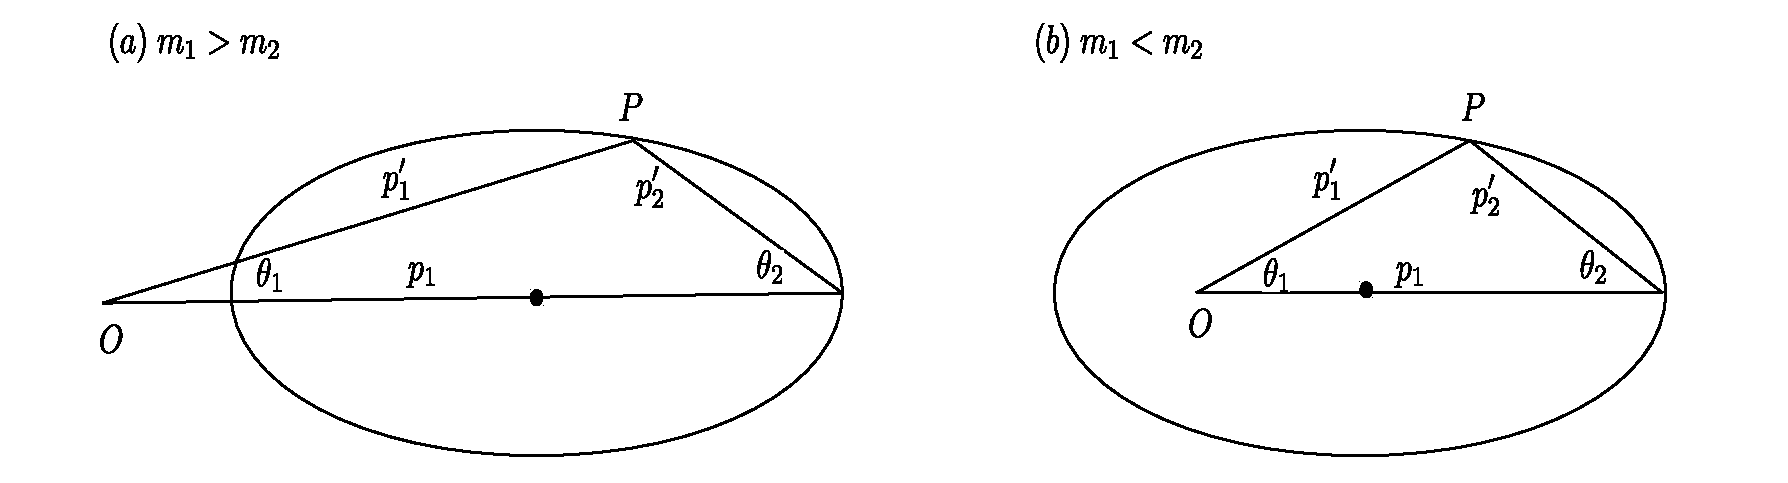
\includegraphics[scale=0.6]{CFT/scattering.eps}
	\caption{Relativistic scattering}
\end{figure}
\noindent
Next, suppose in the center of mass frame (C frame), the scattering angle is $\chi$, we can derive that
\[E_1' = E_1 - \Delta E , \quad E_2' = m_2 + \Delta E,\]
where
\[\Delta E \equiv \frac{m_2(E_1^2-m_1^2)}{m_1^2 + m_2^2 + 2m_2E_1}(1-\cos\chi).\]

\chapter{Classical Field Theory}
\section{Lagrangian formulation}
\[S = \int \mathcal{L}(\phi_a,\dot{\phi}_a,\nabla \phi_a) d^4 x, \ \ \ \ \delta \phi_a |_{\Sigma} = 0.\]
\[\delta S = 0 \Rightarrow \partial_{\mu} \left (\frac{\partial \mathcal{L}}{\partial (\partial_{\mu} \phi_a)} \right ) - \frac{\partial \mathcal{L}}{\partial \phi_a} = 0.\]
\subsubsection{Locality of the theory}
There are no terms in the Lagrangian coupling $\phi(\bm{x},t)$ directly to  $\phi(\bm{y},t)$ with $\bm{x} \neq \bm{y}$. The closet we get for the $\bm{x}$ label is coupling between $\phi(\bm{x},t)$ and $\phi(\bm{x}+\delta\bm{x},t)$ through the gradient term $\bm{\nabla} \phi$.
\subsubsection{Lorentz invariance}

Scalar fields:
\[\overline{\phi}(x) = \phi(\Lambda^{-1} x).\]
Vector fields:
\[\overline{A}^{\mu}(x) = \Lambda^{\mu}_{\phantom{\mu}\nu} A^{\nu}(\Lambda^{-1}x);\]
\[\overline{A}_{\mu}(x) = (\Lambda^{-1})^{\nu}_{\phantom{\mu}\mu} A_{\nu}(\Lambda^{-1}x) = \Lambda_{\mu}^{\phantom{\mu}\nu}A_{\nu}(\Lambda^{-1}x);\]
\[\overline{\partial_{\mu}\phi}(x) = (\Lambda^{-1})^{\nu}_{\phantom{\mu}\mu} \partial_{\nu} \phi (\Lambda^{-1}x) = \Lambda_{\mu}^{\phantom{\mu}\nu} \partial_{\nu} \phi (\Lambda^{-1}x).\]
Lagrangian must be a scalar, or more loosely, action must be invariant under Lorentz transformation.

\section{Symmetry and conservation law}
\begin{newthem}[Noether's theorem]
	Every continuous symmetry of the Lagrangian gives rise to a conserved current $j^{\mu}(x)$ such that the equation of motion imply $\partial_{\mu} j^{\mu} = 0$.
	Suppose that the infinitesimal transformation is
	\[\phi_a \rightarrow \phi_a + \delta \phi_a;\]
	\[\mathcal{L} \rightarrow  \mathcal{L} + \delta \mathcal{L} .\]
	and if $\delta \mathcal{L} = \partial_{\mu} K^{\mu}$, we can get
	\[j^{\mu} = -\frac{\partial \mathcal{L}}{\partial (\partial_{\mu} \phi_a)} \delta \phi_a + K^{\mu}.\]
\end{newthem}

\subsubsection{space-time translation}
$\phi_{a}(x^{\mu}) \to \phi_{a}(x^{\mu}-a^{\mu})$.
\[j^{\mu} = -a_{\nu} T^{\mu \nu},\]
\[T^{\mu \nu} \equiv -\frac{\partial \mathcal{L}}{\partial(\partial_{\mu}\phi_a)} \partial^{\nu} \phi_a + \eta^{\mu \nu} \mathcal{L}.\]
If we define $P^{\mu} \equiv \int T^{0 \mu} d^3 x$, then we have the law of momentum conservation:
\[\frac{d P^{\mu}}{dt} = 0.\]

\subsubsection{Lorentz Transformation}
$\phi_{a}(x^{\mu}) \to \tensor{\mathscr{S}}{_a^b} \phi_{b}(x^{\mu}-\tensor{\delta \omega}{^{\mu}_{\nu}}x^{\nu})$.
\\ \\
The infinitesimal Lorentz transformation can be written as $I+\delta \omega^{\mu}_{\phantom{\mu}\nu}$ and
\[\delta \omega^{\mu}_{\phantom{\mu}\nu} = \left[ 
\begin{matrix} 
0       & \beta_1   & \beta_2   & \beta_3   \\ 
\beta_1 & 0         & -\theta_3 & \theta_2  \\
\beta_2 & \theta_3  & 0         & -\theta_1 \\
\beta_3 & -\theta_2 & \theta_1  & 0
\end{matrix} 
\right].\]
We assume that
\[\overline{\phi}_a(x) = \mathscr{S}_{a}^{\phantom{a}b}\phi_b(\Lambda^{-1}x).\]
In the limit of infinitesimal Lorentz transformation, we have
\[\mathscr{S}_{a}^{\phantom{a}b} = \delta_{a}^{\phantom{a}b}+\frac{1}{2} \delta \omega_{\alpha \beta} (\Sigma^{\alpha \beta})_{a}^{\phantom{a}b} .\]
Therefore,
\[j^{\mu} = \frac{1}{2} M^{\mu \nu \rho}  \delta \omega_{\nu \rho},\]
\[M^{\mu \nu \rho} \equiv x^{\nu}T^{\mu \rho} - x^{\rho} T^{\mu \nu} - \frac{\partial \mathcal{L}}{\partial (\partial_{\mu}\phi_a)}(\Sigma^{\nu \rho})_{a}^{\phantom{a}b}\phi_b.\]
If we define $M^{\nu \rho} \equiv \int M^{0 \nu \rho} d^3 x$, then we have the law of angular momentum conservation:
\[\frac{dM^{\nu \rho}}{dt} = 0.\]

\section{Functional derivatives}
\begin{newdef}[Functional derivatives]
	Given a manifold $M$ representing (continuous/smooth) functions $\rho$ (with certain boundary conditions etc.), and a functional $F$ defined as
	\[F\colon M\rightarrow \mathbb {R}  \quad {\mbox{or}} \quad F\colon M\rightarrow \mathbb {C} ,\]
	the functional derivative of $F[\rho]$, denoted $\frac{\delta F}{\delta \rho}$,is defined by
	\[{\begin{aligned}\int {\frac {\delta F}{\delta \rho }}(x)\phi (x)\;dx&=\lim _{\varepsilon \to 0}{\frac {F[\rho +\varepsilon \phi ]-F[\rho ]}{\varepsilon }}\\&=\left[{\frac {d}{d\epsilon }}F[\rho +\epsilon \phi ]\right]_{\epsilon =0},\end{aligned}}\]
	where $\phi$ is an arbitrary function. The quantity $\epsilon \phi$ is called the variation of $\rho$.
\end{newdef}
\noindent
Like the derivative of a function, the functional derivative satisfies the following properties, where $F[\rho]$ and $G[\rho]$ are functionals:\\
{\bf Linearity}:
\[{\frac {\delta (\lambda F+\mu G)[\rho ]}{\delta \rho (x)}}=\lambda {\frac {\delta F[\rho ]}{\delta \rho (x)}}+\mu {\frac {\delta G[\rho ]}{\delta \rho (x)}},\]
where $\lambda$, $\mu$ are constants.\\
{\bf Product rule}:
\[{\frac {\delta (FG)[\rho ]}{\delta \rho (x)}}={\frac {\delta F[\rho ]}{\delta \rho (x)}}G[\rho ]+F[\rho ]{\frac {\delta G[\rho ]}{\delta \rho (x)}},\]
{\bf Chain rules}:\\
If $F$ is a functional and $G$ an operator, then
\[{\displaystyle \displaystyle {\frac {\delta F[G[\rho ]]}{\delta \rho }(y)}=\int dx{\frac {\delta F[G[\rho]]}{\delta G[\rho]}}(x)\cdot {\frac {\delta G[\rho ]}{\delta \rho}(x,y)}\ }.\]
If $G$ is an ordinary differentiable function $g$, then this reduces to
\[{\displaystyle \displaystyle {\frac {\delta F[g(\rho )]}{\delta \rho}(y)}={\frac {\delta F[g(\rho )]}{\delta g[\rho ]}(y)}\ {\frac {dg(\rho )}{d\rho }(y)}\ } .\]
\begin{newprop}[Properties of functional derivatives]
	\[\frac{\delta F}{\delta \rho} (y) = \lim_{\epsilon \to \infty} \frac{1}{\epsilon} \{ F[\rho + \epsilon \delta_y] - F[\rho] \}, \mbox{ where }\delta_y(x) \equiv \delta(x-y).\]
	\[\frac{\delta f(x)}{\delta f(y)} = \delta(x-y).\]
	\[\frac{\delta}{\delta f(y)} \int g\left( f(t)\right) dt =  g'(f(y)).\]
	\[\frac{\delta f'(x)}{\delta f(y)} = \frac{d}{dx}\delta(x-y).\]
	\[\frac{\delta}{\delta f(y)} \int g\left( f'(t)\right) dt = -\frac{d}{dy} g'(f'(y)).\]
\end{newprop}

\section{Hamiltonian formulation}
\[\pi^a(x) = \frac{\partial \mathcal{L}}{\partial \dot{\phi_a}},\]
\[\mathcal{H}(\phi_a,\nabla \phi_a,\pi^a) = \pi^a \dot{\phi_a} - \mathcal{L},\]
\[H = \int \mathcal{H} d^3 x.\]
Now, we can get the Hamilton equation form $\delta S =0$,
\[\dot{\phi_a}(\bm{x},t) = \frac{\delta}{\delta \pi^a(\bm{x},t)} H = \frac{\partial \mathcal{H}}{\partial \pi^a};\]
\[\dot{\pi^a}(\bm{x},t) = -\frac{\delta}{\delta \phi_a(\bm{x},t)} H = - \frac{\partial \mathcal{H}}{\partial \phi_a} + \left(\frac{\partial \mathcal{H}}{\partial \phi_{a,b}}\right)_{,b}.\]

\subsection{Poisson bracket}

First, we define that
\[[\phi_a(\bm{x}),\phi_b(\bm{y})] \equiv [\pi^a(\bm{x}),\pi^b(\bm{y})] \equiv 0,\]
\[[\phi_a(\bm{x}),\pi^b(\bm{y})] \equiv \delta^{b}_{a} \delta(\bm{x}-\bm{y}).\]
Then, we demand that the bracket operation has the same properties as the Poisson bracket in classical mechanics. And we also demand that
\[[\partial_x A(\bm{x}),B(\bm{y})] = \partial_x [A(\bm{x}),B(\bm{y})]\]
and
\[\left[\int d^3 x A(\bm{x}),B(\bm{y})\right] = \int d^3 x [A(\bm{x}),B(\bm{y})].\]
As a result, we can verify that
\[[W[\phi(\bm{x}),\pi(\bm{x})],Z[\phi(\bm{x}),\pi(\bm{x})]] = \int d^3x \left\{ \frac{\delta W}{\delta \phi(\bm{x})} \frac{\delta Z}{\delta \pi(\bm{x})} - \frac{\delta W}{\delta \pi(\bm{x})} \frac{\delta Z}{\delta \phi(\bm{x})} \right\}.\]
Especially,
\[[\phi_a(\bm{x}),H] = \frac{\delta }{\delta \pi^a(\bm{x})} H, \ \ \ \ [\pi^a(\bm{x}),H] = -\frac{\delta }{\delta \phi_a(\bm{x})} H.\]
Therefore, the Hamilton equation can be written as
\[\dot{\phi_a} = [\phi_a,H], \ \ \ \ \dot{\pi^a} = [\pi^a,H].\]
Further more, we can prove that
\[\frac{dO(\phi,\pi,t)}{dt} = [O,H] + \frac{\partial O}{\partial t} \]
and
\[\frac{d[A,B]}{dt} = [A,\frac{dB}{dt}] + [\frac{dA}{dt},B]  .\]

\subsection{Momentum}

It is easy to verify that
\[P^{0} = H, \ \ \ \ P^{i} = \int -\pi^a \partial^i \phi_a d^3 x.\]
And we can get the Poisson bracket
\begin{eqnarray}
	\left[\phi_a,P^{\mu}\right] &=& -\partial^{\mu} \phi_a, \nonumber \\
	\left[\pi^a,P^{\mu}\right] &=& -\partial^{\mu} \pi^a, \nonumber \\
	\left[P^{\mu},P^{\nu}\right] &=& 0 .\nonumber 
\end{eqnarray}

\subsection{Angular momentum}
It is easy to verify that
\[M^{\mu \nu} = \int (x^{\mu}T^{0\nu}-x^{\nu}T^{0\mu}-\pi^a(\Sigma^{\mu \nu})_{a}^{\phantom{a}b}\phi_b) d^3 x.\]
We define that
\[M_{\rm L}^{\mu \nu} \equiv \int (x^{\mu}T^{0\nu}-x^{\nu}T^{0\mu}) d^3 x , \quad M_{\rm S}^{\mu \nu} \equiv \int (-\pi^a(\Sigma^{\mu \nu})_{a}^{\phantom{a}b}\phi_b) d^3 x.\]
\[(\mathcal{L}^{\mu \nu})_a^{\phantom{a}b} \equiv -(x^{\mu}\partial^{\nu}-x^{\nu}\partial^{\mu})\delta_a^{\phantom{a}b} , \quad (\mathcal{S}^{\mu \nu})_a^{\phantom{a}b} \equiv -(\Sigma^{\mu \nu})_a^{\phantom{a}b}.\]
Therefore, we can get the Poisson bracket
\[[\phi_a,M_{\rm L}^{\mu \nu}] = (\mathcal{L}^{\mu \nu})_a^{\phantom{a}b} \phi_b , \quad [\phi_a,M_{\rm S}^{\mu \nu}] = (\mathcal{S}^{\mu \nu})_a^{\phantom{a}b} \phi_b.\]
\[[\pi^a,M_{\rm L}^{\mu \nu}] = (\mathcal{L}^{\mu \nu})_b^{\phantom{b}a}\pi^{b}  , \quad [\pi^a,M_{\rm S}^{\mu \nu}] = - (\mathcal{S}^{\mu \nu})_b^{\phantom{b}a} \pi^b .\]
Because ${d M^{\mu \nu}}/{dt} = 0$, $M^{\mu \nu}$ can commutate with ${d}/{dt}$, so
\[[[\phi(x),M^{\mu \nu}],M^{\rho \sigma}] = (\mathcal{L}^{\mu \nu}+\mathcal{S}^{\mu \nu})(\mathcal{L}^{\rho \sigma}+\mathcal{S}^{\rho \sigma})\phi(x).\]
At last, we can get the Poisson bracket 
\[[\phi(x),[M^{\mu \nu},M^{\rho \sigma}]] = (\mathcal{L}^{\mu \nu}\mathcal{L}^{\rho \sigma}-\mathcal{L}^{\rho \sigma}\mathcal{L}^{\mu \nu} + \mathcal{S}^{\mu \nu}\mathcal{S}^{\rho \sigma}-\mathcal{S}^{\rho \sigma}\mathcal{S}^{\mu \nu})\phi(x).\]
Since we can prove that
\[\mathcal{L}^{\mu \nu}\mathcal{L}^{\rho \sigma}-\mathcal{L}^{\rho \sigma}\mathcal{L}^{\mu \nu} = -\eta^{\nu \rho}\mathcal{L}^{\mu \sigma} + \eta^{\sigma \mu}\mathcal{L}^{\rho \nu} + \eta^{\mu \rho}\mathcal{L}^{\nu \sigma} - \eta^{\sigma \nu}\mathcal{L}^{\rho \mu}.\]
If we demand that
\[\mathcal{S}^{\mu \nu}\mathcal{S}^{\rho \sigma}-\mathcal{S}^{\rho \sigma}\mathcal{S}^{\mu \nu} = -\eta^{\nu \rho}\mathcal{S}^{\mu \sigma} + \eta^{\sigma \mu}\mathcal{S}^{\rho \nu} + \eta^{\mu \rho}\mathcal{S}^{\nu \sigma} - \eta^{\sigma \nu}\mathcal{S}^{\rho \mu},\]
we will get get the Poisson bracket of the $M^{\mu \nu}$,
\[[M^{\mu \nu},M^{\rho \sigma}] = -\eta^{\nu \rho}M^{\mu \sigma} + \eta^{\sigma \mu}M^{\rho \nu} + \eta^{\mu \rho}M^{\nu \sigma} - \eta^{\sigma \nu}M^{\rho \mu},\]
up to the possibility of a term on the right-hand side that commutes with $\phi(x)$ and its derivatives.
\\ \\
We now define $J_i \equiv 1/2 \; \epsilon_{ijk} M^{jk}$ and $K_i \equiv M^{i0}$, so we have
\[M^{\mu \nu} = \left[ 
\begin{matrix} 
0   & -K_1 & -K_2 & -K_3 \\ 
K_1 & 0    & J_3  & -J_2 \\
K_2 & -J_3 & 0    &  J_1 \\
K_3 & J_2  & -J_1 &  0
\end{matrix} 
\right] , \quad \left( 
\delta \omega_{\mu\nu} = \left[
\begin{matrix} 
0       & -\beta_1   & -\beta_2   & -\beta_3   \\ 
\beta_1 & 0         & -\theta_3 & \theta_2  \\
\beta_2 & \theta_3  & 0         & -\theta_1 \\
\beta_3 & -\theta_2 & \theta_1  & 0
\end{matrix} 
\right] \right).\] 
the Poisson bracket can be written as
\begin{eqnarray}
	\left[J_i,J_j\right] &=& \epsilon_{ijk}J_k , \nonumber \\
	\left[J_i,K_j\right] &=& \epsilon_{ijk}K_k ,\nonumber \\
	\left[K_i,K_j\right] &=& -\epsilon_{ijk}J_k .\nonumber
\end{eqnarray}
We can use the similar method to derive that
\[[P^{\mu},M^{\rho \sigma}] = \eta^{\mu \sigma}P^{\mu} - \eta^{\mu \rho}P^{\sigma}.\]
It can also be written as
\begin{eqnarray}
	\left[J_i,H\right] &=& 0 ,\nonumber \\
	\left[J_i,P_j\right] &=& \epsilon_{ijk}P_k, \nonumber \\
	\left[K_i,H\right] &=& P_i ,\nonumber \\
	\left[K_i,P_j\right] &=& \delta_{ij}H .\nonumber
\end{eqnarray}
At last, we define $L_i \equiv 1/2 \; \epsilon_{ijk} M_{\rm L}^{jk}$ and $S_i \equiv 1/2 \; \epsilon_{ijk} M_{\rm S}^{jk}$
we can demonstrate that
\begin{eqnarray}
	\left[L_i,S_j\right] &=& 0 ,\nonumber \\
	\left[S_i,P_j\right] &=& 0, \nonumber \\
	\left[L_i,P_j\right] &=& \epsilon_{ijk}P_k . \nonumber
\end{eqnarray}

\chapter{Classical Electrodynamics}
\section{The formulation of classical electrodynamics}
\subsection{Maxwell equations and Lorentz force}
The Lagrangian of the EM field $A^{\mu}$ when coupling with current is
\[\mathcal{L} = -\frac{1}{4}F^{\mu\nu}F_{\mu\nu} + j^{\mu} A_{\mu},\]
where
\[F_{\mu\nu} \equiv \partial_{\mu}A_{\nu} - \partial_{\nu}A_{\mu} , \quad j^{\mu} \equiv \rho_{\mathrm{e}0} u^{\mu},\]
and $\rho_{\mathrm{e}0}$ is the charge density measured in the frame of charge.
The Euler-Lagrange equation of EM field is
\[\partial_{\nu} F^{\mu\nu} = j^{\mu}.\]
The charge conservation equation then follows directly from field equations,
\[\partial_{\mu} j^{\mu} = \partial_{\mu} \partial_{\nu} F^{\mu\nu} = 0.\]
For a charged particle moving in EM field with trajectory $x^{\mu}(\tau)$, we have
\[j^{\mu} =  e_a \delta(\bm{r}-\bm{r}_a(t)) \sqrt{1-\bm{v}_a^2} u_a^\mu .\]
It follows that
\[\int dV dt j^{\mu} A_{\mu} = \int dx^{\mu} e_a A_{\mu}(x^{\mu}(\tau)).\]
Thus the action for a charged particle when coupling with EM field is
\[S = - m \int d\tau + e\int dx^{\mu} A_{\mu}(x^{\mu}(\tau)).\]
We can derive the Euler-Lagrangian equation of the particle:
\[ma_{\mu} = eF_{\mu \nu}u^{\nu}.\]
\begin{note}
The Hamiltonian formulation of electrodynamics will be discussed in detail in the Hamiltonian formulation of general relativity and canonical quantization formulation of quantum electrodynamics.
\end{note}
\noindent
We now define the electric field and magnetic field as follows,
\[E^i \equiv F^{0i} = -\dot{A}^i - \nabla^i A^0 , \quad B^i \equiv \epsilon_{ijk} \nabla^j A^k.\]
We also define $\rho_{\mathrm{e}} \equiv j^0$ and $J^i \equiv j^i$,so
the field equations can then be written as so-called Maxwell equations:
\begin{eqnarray}
	\bm{\nabla} \times  \bm{B} &=& \frac{\partial \bm{E}}{\partial t} +  \bm{J} ,\nonumber \\
	\bm{\nabla} \times \bm{E} &=& -\frac{\partial \bm{B}}{\partial t} ,\nonumber \\
	\bm{\nabla} \cdot \bm{E} &=& \rho_{\mathrm{e}}, \nonumber \\
	\bm{\nabla} \cdot \bm{B} &=& 0 .\nonumber
\end{eqnarray}
The equations of motion of the charged particle can be written as so-called Lorentz force equations:
\[\frac{d\bm{p}}{dt} = e(\bm{E} + \bm{v} \times \bm{B}) , \quad \frac{d \mathcal{E}}{dt} = e \bm{E} \cdot \bm{v}.\]
\\
We also note that $A_{\mu}$ cannot be completely determined by Maxwell and Lorentz equation. If we make the transformation $A_{\mu} \to A_{\mu} + \partial_{\mu} \xi(x)$, $\mathcal{L}$ and $F^{\mu\nu}$ would be invariant, and the Maxwell and Lorentz equation is still valid. This arbitrariness of $\xi$ is called gauge invariance. The topic will be discussed in detail in QED.

\subsection{Lorentz transformation of fields}
Suppose the new coordinates satisfy that $\overline{x}^{\mu} = \Lambda^{\mu}_{\phantom{\mu}\nu}x^{\nu}$ after Lorentz transformation, then we have
\[\overline{A}^{\mu}(\overline{x}) = \Lambda^{\mu}_{\phantom{\mu}\nu}A^{\nu}(\Lambda^{-1}\overline{x}).\]
In a special case where the new reference frame move along $\hat{1}$ direction with velocity $\beta$, we have
\[\overline{x}^{0} = \gamma x^0 - \gamma \beta x^1 , \quad \overline{x}^{1} = -\gamma \beta x^0 + \gamma x^1.\]
Similarly, for vector potential, we have 
\[\overline{A}^{0} = \gamma A^0 - \gamma \beta A^1 , \quad \overline{A}^{1} = -\gamma \beta A^0 + \gamma A^1.\]
It can be further written in terms of electric and magnetic field as
\[\overline{E}_1 = E_1 , \quad \overline{E}_2 = \gamma E_2 - \gamma \beta B_3 , \quad \overline{E}_3 = \gamma E_3 + \gamma \beta B_2,\]
\[\overline{B}_1 = B_1 , \quad \overline{B}_2 = \gamma B_2 + \gamma \beta E_3 , \quad \overline{B}_3 = \gamma B_3 - \gamma \beta E_2,\]
or more generally as
\[\bm{\overline{E}} = \gamma(\bm{E}_{\perp} + \bm{\beta} \times \bm{B}) + \bm{E}_{\parallel},\]
\[\bm{\overline{B}} = \gamma(\bm{B}_{\perp} - \bm{\beta} \times \bm{E}) + \bm{B}_{\parallel}.\]
If $\beta \ll 1$, we can neglect the higher order of $\beta^2$. Therefore, we have
\[\bm{\overline{E}} = \bm{E} + \bm{\beta} \times \bm{B};\]
\[\bm{\overline{B}} = \bm{B} - \bm{\beta} \times \bm{E}.\]
We also note that $F_{\mu\nu}F^{\mu\nu}$ and $\epsilon_{\mu\nu\rho\sigma}F^{\mu\nu}F^{\rho\sigma}$ is invariant under Lorentz transformation. It can be represented by the electric and magnetic field as
\[E^2 - B^2 = \mbox{ inv } , \quad \bm{E} \cdot \bm{B} = \mbox{ inv }.\]

\subsection{Energy-momentum tensor}
For a free EM field, the energy-momentum tensor is
\[T_{\mathrm{f}}^{\mu \nu} \equiv -\frac{\partial \mathcal{L}}{\partial(\partial_{\mu}A_{\rho})} \partial^{\nu} A_{\rho} + \eta^{\mu \nu} \mathcal{L} = \partial^{\nu}A^{\rho} F^{\mu}_{\phantom{\rho}\rho}-\frac{1}{4}\eta^{\mu\nu}F_{\rho\sigma}F^{\rho\sigma}.\]
We note that the energy-momentum tensor defined above is not symmetric, so we define a modified energy-momentum tensor by adding a term $-\partial^{\rho}A^{\nu}F^{\mu}_{\phantom{\rho}\rho}$,i.e.
\[T_{\mathrm{f}'}^{\mu\nu} = F^{\nu\rho}F^{\mu}_{\phantom{\rho}\rho}-\frac{1}{4}\eta^{\mu\nu}F_{\rho\sigma}F^{\rho\sigma}.\]
For free EM field, we have $\partial^{\rho}A^{\nu}F^{\mu}_{\phantom{\rho}\rho} = \partial^{\rho}\left(A^{\nu} F^{\mu}_{\phantom{\rho}\rho}\right)$.
Therefore,
\[\partial_{\mu}T_{\mathrm{f}'}^{\mu\nu} = 0 , \quad P_{\mathrm{f}'}^{\mu} = P_{\mathrm{f}}^{\mu}.\]
From now on, we will use $T_{\mathrm{f}'}$ as the energy-momentum tensor of EM field and omit the prime for simplicity.
The momentum of the free EM field is
\[P_{\mathrm{f}}^{0} = \int dV \frac{1}{2}(\bm{E}^2+\bm{B}^2) \equiv \int dV w , \quad P_{\mathrm{f}}^{i} = \int dV \bm{E} \times \bm{B} \equiv \int dV \bm{S}.\]
\\ \\
If there also exists charged particles in the system, i.e. the source of EM field, we must also include the energy-momentum tensor of the particles to get the right conservation equation. The energy-momentum tensor of particles is defined as
\[T_{\mathrm{p}}^{\mu\nu} \equiv \sum_a m_a \delta(\bm{r}-\bm{r}_a) \sqrt{1-\bm{v}_a^2} u_a^\mu u_a^{\nu}.\]
From this definition, we can get
\[P_{\mathrm{p}}^0 = \sum_a \frac{m_a}{\sqrt{1-\bm{v}_a^2}} , \quad \bm{P}_{\mathrm{p}} =  \sum_a \frac{m_a}{\sqrt{1-\bm{v}_a^2}} \bm{v}_a.\]
Recall that
\[j^{\mu}_{\mathrm{e}} = \sum_a e_a \delta(\bm{r}-\bm{r}_a) \sqrt{1-\bm{v}_a^2} u_a^\mu .\]
We can also define the mass current as
\[j^{\mu}_{\mathrm{m}} \equiv \sum_a m_a \delta(\bm{r}-\bm{r}_a) \sqrt{1-\bm{v}_a^2} u_a^\mu .\]
If there is no creation and annihilation of charged particles, and the mass of the particles is constant during the motion, we would have mass conservation equation
\[\partial_{\mu} j^{\mu}_{\mathrm{m}a} = 0.\]
Recall the Lorentz force equation $m a_{\mu} = eF_{\mu\nu}u^{\nu}$, it can be rewritten as
\[\rho_{\mathrm{m}0a} \frac{du_{\mu}}{d\tau} = F_{\mu\nu}j_{\mathrm{e}a}^{\nu}.\]
where $\rho_{\mathrm{m}0a} \equiv m_a \delta(\bm{r}-\bm{r}_a) \sqrt{1-\bm{v}_a^2}$ is the mass density measured in the rest frame of the particle.
On the one hand, we have
\[\partial_{\mu} T_{\mathrm{p}}^{\mu\nu} = \sum_a \rho_{\mathrm{m}0a}u^{\mu} \frac{\partial u_a^{\nu}}{\partial x^{\mu}} = \sum_a \rho_{\mathrm{m}0a} \frac{d u_a^{\nu}}{d \tau} = F^{\nu}_{\phantom{\nu}\mu}j_{\mathrm{e}}^{\mu}.\]
On the other hand, we can derive that
\[\partial_{\mu} T_{\mathrm{f}}^{\mu\nu} = - F^{\nu}_{\phantom{\nu}\mu}j_{\mathrm{e}}^{\mu}\]
by implementing Maxwell equations.
Define
\[T^{\mu \nu} \equiv T_{\mathrm{f}}^{\mu\nu} + T_{\mathrm{p}}^{\mu\nu}.\]
We have
\[\partial_{\mu} T^{\mu\nu} = 0.\]
We define the Maxwell stress tensor as
\[f^{ij} \equiv -T_{\mathrm{f}}^{ij} = E^{i}E^{j} + B^{i}B^{j} - w\delta^{ij}.\]
Then, we can write down the conservation laws of energy and momentum as
\[\frac{d}{dt}\left(P_{\mathrm{p}}^0 + \int w dV \right) = -\oint \bm{S}\cdot d\bm{\sigma},\]
\[\frac{d}{dt}\left(\bm{P}_{\mathrm{p}} + \int \bm{S} dV \right) = \oint \bm{f}\cdot d\bm{\sigma}.\]
We assume there is no particle cross the boundary.
Because $T^{\mu\nu} = T^{\nu\mu}$, we have
\[\partial_{\mu}(x^{\nu}T^{\mu\rho}-x^{\rho}T^{\mu\nu}) = 0.\]
It is easy to write down the conservation law of angular momentum as
\[\frac{d}{dt}\left(\bm{L}_{\mathrm{p}} + \int \bm{r} \times \bm{S} dV \right) = \oint \bm{r} \times \bm{f}\cdot d\bm{\sigma},\]
where
\[\bm{L}_{\mathrm{p}} \equiv \sum_a \frac{m_a}{\sqrt{1-\bm{v}_a^2}} \bm{r}_a  \times \bm{v}_a .\]

\subsection{Charged particles in a given EM field}
Now we suppose the EM field is given, i.e. we will neglect the EM field generated by the test charged particles. Then we have
\[S = \int_{t_1}^{t_2} (-\sqrt{1-v^2}m + e\bm{A}\cdot\bm{v}-e\phi)dt.\]
Thus
\[L = -\sqrt{1-v^2}m + e\bm{A}\cdot\bm{v}-e\phi.\]
The canonical momentum is
\[\bm{\pi} = \frac{\partial L}{\partial \bm{v}} = \gamma m \bm{v} + e \bm{A}.\]
The Hamiltonian is therefore
\[H = \bm{\pi} \cdot \bm{v} - L = \gamma m + e \phi = \sqrt{m^2+(\bm{\pi}-e\bm{A})^2}+e\phi.\]
If $v \ll 1$, we have
\[L = \frac{mv^2}{2} + e\bm{A}\cdot\bm{v}-e\phi , \quad \bm{\pi} =  m \bm{v} + e \bm{A} , \quad H = \frac{(\bm{\pi}-e\bm{A})^2}{2m}+e\phi.\]
If the EM field is constant in time, we have
\[\bm{\nabla} \times \bm{E} = 0 ,\]
and we could choose the gauge that
\[\dot{\bm{A}} = 0 , \quad \bm{E} = -\bm{\nabla} \phi.\]
Because $\partial L/{\partial t}=0$, $\gamma m + e\phi$ is a constant.

\subsubsection{Motion in a uniform and constant electric field}
Suppose the direction of electric field is  $\hat{x}$, the orbit is in the $x-y$ plane. Therefore, the equation of motion is
\[\dot{p}_x = eE , \quad \dot{p}_y = 0.\]
The final solution is
\[x = \frac{1}{eE}\sqrt{\mathcal{E}_0^2 + (eEt)^2} , \quad y = \frac{p_0}{eE} \mathrm{arcsinh} \frac{eEt}{\mathcal{E}_0}.\]
Here, we assume $p_x = 0$, $p_y=p_0$ at $t = 0$ and $\mathcal{E}_0 \equiv \sqrt{p_0^2+m^2}$.
The trajectory of the particle is
\[x = \frac{\mathcal{E}_0}{eE}\cosh \frac{eEy}{p_0}.\]

\subsubsection{Motion in a uniform and constant magnetic field}
Suppose the direction of magnetic field is $\hat{z}$. Note that particle's kinetic energy $\mathcal{E} = \gamma m$ is constant if there are no electric field, we can derive the equation of motion
\[\dot{v}_x = \omega v_y , \quad \dot{v}_y = -\omega v_x , \quad \dot{v}_z = 0,\]
where $\omega \equiv {eB}/{\gamma m}$. The final solution is
\[x = x_0 + r\sin(\omega t + \alpha) , \quad y = y_0 + r\cos(\omega t + \alpha) , \quad z = z_0 + v_{0z}t.\]
where $x_0,y_0,z_0,r,\alpha,v_{0z}$ should be determined by initial condition.

\subsubsection{Motion in a uniform and constant EM field}
We only focus on the case where the velocity of particle is much smaller than the velocity of light. 
Suppose the direction of magnetic field is $\hat{z}$, the direction of electric field is within $y-z$ plane. The equation of motion is
\[m\ddot{x} = eB\dot{y} , \quad m\ddot{y} =eE_y - eB\dot{x} , \quad m\ddot{z}=eE_z.\]
The solution is
\[\dot{x} = a \cos \omega t + \frac{E_y}{B} , \quad \dot{y} = -a\sin \omega t , \quad \dot{z} = v_{0z} + \frac{eE_z}{m}t.\]
where $\omega = {eB}/{m}$ , $a,v_{z0}$ is determined by initial condition. As we suppose that $v \ll 1$ is satisfied,we must have that
\[a \ll 1 , \quad v_{0z} \ll 1 , \quad \frac{eE_z t}{m} \ll 1 , \quad \frac{E_y}{B} \ll 1.\]

\section{Constant electromagnetic field}
\subsection{Coulomb' law}
For constant electric field, Maxwell equations take the form 
\[\bm{\nabla} \cdot \bm{E} = \rho_{\mathrm{e}} , \quad \bm{\nabla} \times \bm{E} = 0.\]
Therefore, we have
\[\bm{E} = -\bm{\nabla} \phi , \quad \nabla^2 \phi = -\rho_{\mathrm{e}} .\]
The solution is
\[\phi(\bm{r}) = \int  \frac{\rho_{\mathrm{e}}(\bm{r}')}{4\pi|\bm{r}-\bm{r}'|} dV'.\]
If $\rho_{\mathrm{e}}(\bm{r}') = Q \delta(\bm{r}')$, we have
\[\phi(\bm{r}) =  \frac{Q}{4\pi|\bm{r}|} , \quad E(\bm{r}) = \frac{Q\bm{r}}{4\pi|\bm{r}|^3}.\]
For a system of static charged particles, the total energy is
\[U = \frac{1}{2}\int E^2 dV = \frac{1}{2} \int \rho \phi dV = \frac{1}{2} \sum e_a \phi_a + \frac{1}{2}\sum e_a \Phi_a.\]
Here, $\phi_a$ is the electric potential at the point where $e_a$ is located, produced by $e_a$ itself, while  $\Phi_a$ is the potential produced by other charges. It is obvious that $U_{\mathrm{self}} =  e_a \phi_a/2$ is infinite, indicating that classical electrodynamics is no more valid in small distance. This problem will be solved in quantum electrodynamics: the mass of charged particle we measured is already renormalized to include the electromagnetic self energy. Therefore, actually, we have
\[U = \frac{1}{2}\int E^2 dV - U_{\mathrm{self}} = \frac{1}{2}\sum_{a \ne b} \frac{e_a e_b}{4\pi R_{ab}}.\]
If the charged particle is moving with a constant velocity, we can derive the electric field it produced by Lorentz transformation, the final result is that
\[\bm{E} = \frac{e\bm{R}}{4\pi R^3} \frac{1-V^2}{(1-V^2\sin^2\theta)^{3/2}} , \quad \bm{B} = \bm{V} \times \bm{E},\]
where $\bm{R}$ is the vector point from the particle to the point we measure the electric field, and $\theta$ is the angle between $\bm{V}$ and $\bm{R}$.
If $V \sim 1$, the electric field will be concentrated in the direction perpendicular to the $\bm{V}$. If $\bm{V} \ll 1$, we have
\[\bm{E} = \frac{e\bm{R}}{4\pi R^3} , \quad \bm{B} = \frac{e\bm{V} \times\bm{R}}{4\pi R^3}.\]

\subsection{Multipole moments}
For a system of charged particles, the potential it produced at $\bm{R}$ is
\[\phi = \sum_a \frac{e_a}{4\pi|\bm{R} - \bm{r}_a|}.\]
If $R \gg r_a$, we can expand the equation around $r_a=0$. Generally, we have
\[\frac{1}{|\bm{R} - \bm{r}|} = \sum_{l=0}^{\infty} \sum_{m=-l}^{l} \frac{r^l}{R^{l+1}} \frac{4\pi}{2l+1} Y^*_{lm}(\Theta,\Phi)Y_{lm}(\theta,\phi).\]
Thus
\[\phi = \sum \phi^{(l)},\]
where
\[\phi^{(l)} \equiv \frac{1}{4\pi R^{l+1}} \sum_{m=-l}^{l} \sqrt{\frac{4\pi}{2l+1}} Q_{m}^{(l)} Y^*_{lm}(\Theta,\Phi).\]
\[Q_m^{(l)} \equiv \sum_a e_a r_a^l \sqrt{\frac{4\pi}{2l+1}} Y_{lm}(\theta_a,\phi_a).\]
Leading terms: 
\[\phi^{(0)} = \frac{Q}{4\pi R} , \quad E^{(0)} = \frac{Q\bm{n}}{4\pi R^2} , \quad Q = \sum_a e_a.\]
\[\phi^{(1)} = \frac{\bm{d} \cdot \bm{n}}{4\pi R^2}  , \quad E^{(1)} = \frac{3(\bm{d}\cdot\bm{n})\bm{n}-\bm{d}}{4\pi R^3} , \quad \bm{d} = \sum_a e_a \bm{r}_a.\]
\[\phi^{(2)} = \frac{\bm{n} \cdot \bm{D} \cdot \bm{n}}{8\pi R^3} , \quad E^{(2)} = \frac{5(\bm{n} \cdot \bm{D} \cdot \bm{n})\bm{n} - (\bm{n} \cdot \bm{D} + \bm{D} \cdot \bm{n})}{8\pi R^4} , \quad D_{ij} = \sum e(3x_ix_j-r^2\delta_{ij}).\]
For a system of charged particles in the electric field $\phi(\bm{r})$, if all the particles is near the $r=0$, we can make the expansion
\[\phi(\bm{r}) = \sum_{l=0}^{\infty} r^l \sum_{m=-l}^{m=l} a_{lm} \sqrt{\frac{4\pi}{2l+1}} Y_{lm}(\theta,\phi).\]
Thus
\[U = \sum_{l=0}^{\infty} U^{(l)} , \quad U^{(l)} = \sum_{m=-l}^{l} a_{lm}Q^{(l)}_m.\]
Leading terms: 
\[U^{(0)} = Q\phi_0 , \quad F^{(0)} = Q\bm{E}_0.\]
\[U^{(1)} = -\bm{d}\cdot \bm{E}_0 , \quad F^{(1)} = \bm{d}\cdot \bm{\nabla}\bm{E}_0 , \quad M^{(1)} = \bm{d} \times \bm{E}_0.\]
\[U^{(2)} = -\frac{1}{6}\bm{D}\cdot \bm{\nabla}\bm{E}_0 , \quad F^{(2)} = \frac{1}{6} \bm{D}\cdot \bm{\nabla}\bm{\nabla}\bm{E}_0 , \quad M^{(2)} = \frac{1}{3} \bm{\nabla} \cdot (\bm{D} \times \bm{E}_0).\]

\subsection{Biot-Savart law}
Let us consider the magnetic field produced by charges which perform a finite motion, in which the particles are always within a finite region of space and the momenta also always remains finite. Consider the time average magnetic field $\overline{\bm{B}}$ , produced by the charges; this field will now be a function only of the coordinates and not of the time. We take the time average of the Maxwell equations
\[\bm{\nabla} \cdot \bm{B} = 0 , \quad \bm{\nabla} \times \bm{B} = \frac{\partial \bm{E}}{\partial t} + \bm{j}.\] 
Note that the average value of the derivative $\partial \bm{E} / \partial t$, like the derivative of any quantity which varies over a finite range, is zero. We can get
\[\bm{\nabla} \cdot \overline{\bm{B}} = 0 , \quad \bm{\nabla} \times \overline{\bm{B}} =  \overline{\bm{j}}.\]
Recall that $\bm{B} = \bm{\nabla} \times \bm{A}$. We impose the gauge condition $\bm{\nabla} \cdot \bm{A} = 0$, we have
\[\nabla^2 \overline{\bm{A}} = - \overline{\bm{j}}.\]
The solution is
\[\overline{\bm{A}}(\bm{r}) = \frac{1}{4\pi} \int \frac{\overline{\bm{j}}(\bm{r}')}{|\bm{r}-\bm{r}'|} dV' = \frac{1}{4\pi} \sum \overline{\frac{e_a \bm{v}_a}{|\bm{r}-\bm{r}_a|}}.\]
And the magnetic field is
\[\overline{\bm{B}}(\bm{r}) = \frac{1}{4\pi} \int \frac{\overline{\bm{j}}(\bm{r}') \times \bm{R}}{R^3} dV' , \quad \bm{R} = \bm{r}-\bm{r}'.\]

\subsection{Magnetic moment}
For a system of charged particles, the potential it produced at $\bm{R}$ is
\[\overline{\bm{A}} = \frac{1}{4\pi} \sum \overline{\frac{e_a \bm{v}_a}{|\bm{R}-\bm{r}_a|}}.\]
If $R \gg r_a$, we can expand the equation around $r_a=0$ the first order,
\[4\pi \overline{\bm{A}} = \frac{1}{R} \sum e \overline{\bm{v}} - \sum \overline{e \bm{v} \left( \bm{r} \cdot \bm{\nabla} \frac{1}{R}\right)}.\]
Firstly,
\[\sum e \overline{\bm{v}} = \overline{\frac{d}{dt} \sum e \bm{r}} = 0.\]
Secondly,
\[-\sum \overline{e \bm{v} \left( \bm{r} \cdot \bm{\nabla} \frac{1}{R}\right)} = \frac{1}{R^3} \sum \overline{e\bm{v} (\bm{r} \cdot \bm{R})}.\]
Note that
\[\sum e\bm{v} (\bm{r} \cdot \bm{R}) = \frac{1}{2} \frac{d}{dt} e\bm{r}(\bm{r}\cdot\bm{R}) + \frac{1}{2} \left(\sum e \bm{r} \times \bm{v}\right) \times \bm{R}.\]
Define the magnetic moment as
\[\bm{m} \equiv \frac{1}{2} \left(\sum e \bm{r} \times \bm{v}\right).\]
We can get
\[\overline{\bm{A}} = \frac{\overline{\bm{m}} \times \bm{R}}{4\pi R^3} , \quad \overline{\bm{B}} = \frac{3\bm{n}(\overline{\bm{m}} \cdot \bm{n})-\overline{\bm{m}}}{4\pi R^3}.\]
If all the particles have the same charge-mass ratio, and the velocity of all the particles is much smaller than that of light, we have
\[\bm{m} = \frac{e}{2m} \sum m \bm{r} \times \bm{v} = \frac{e}{2m} \bm{M}.\]
Let us consider a system of charges in an external constant uniform magnetic field. The time average of the force acting on the system, 
\[\bm{F} = \sum e \overline{\bm{v} \times \bm{B}} = \overline{\frac{d}{dt} \sum e \bm{r} \times \bm{B}} = 0.\]
The average value of the moment of the forces is 
\[\overline{\bm{K}} = \sum e \overline{\bm{r} \times (\bm{v} \times \bm{B})}.\]
We can derive that
\[\overline{\bm{K}} = \overline{\bm{m}} \times \bm{B}.\]
Let us consider the change in the average angular momentum $\overline{\bm{M}}$ of the system. According to a well-known equation of mechanics, the derivative of $\bm{M}$ is equal to the moment $\bm{K}$ of the forces acting on the system. We therefore have
\[\frac{d \overline{\bm{M}}}{dt} = \overline{\bm{m}} \times \bm{B}.\]
If the charge-mass ratio is the same for all particles of the system, the angular momentum and magnetic moment are proportional to one another, and we find:
\[\frac{d \overline{\bm{M}}}{dt} = - \bm{\Omega} \times \overline{\bm{M}} , \quad \bm{\Omega} = \frac{e}{2m} \bm{B}.\]
This equation states that the vector $\overline{\bm{M}}$ rotates with angular velocity $-\bm{\Omega}$ around the direction of the field, while its absolute magnitude and the angle which it makes with this direction remain fixed. This motion is called the Larmor precession.

\section{Electromagnetic waves}
\subsection{Electromagnetic waves}
Electromagnetic fields occurring in vacuum in the absence of  charges are called electromagnetic waves. We choose the Coulomb's Gauge, i.e.
\[ \phi = 0 , \quad \bm{\nabla} \cdot \bm{A} = 0.\]
Therefore,
\[\bm{E} = -\frac{\partial \bm{A}}{\partial t} , \quad \bm{B} = \bm{\nabla} \times \bm{A}.\]
From Maxwell equations we can derive that
\[\nabla^2 \bm{A} - \frac{\partial^2 \bm{A}}{\partial t^2} = 0.\]
This is the equation which determines the potentials of electromagnetic waves. It is called the d'Alembert equation, or the wave equation. We can verify that the electric and magnetic fields $\bm{E}$ and $\bm{B}$ satisfy the same wave equation.
\\ \\
We consider the special case of electromagnetic waves in which the fields depends only on one coordinates, say $x$. Such waves are said to be plane. In this case the equation of the field becomes
\[\frac{\partial^2 f}{\partial t^2}  - \frac{\partial^2 f}{\partial x^2} = 0.\]
The solution is
\[f(t,x) = f_1(t-x) + f_2(t+x).\]
$f_1(t-x)$ represents a plane wave moving in the positive direction along the $x$ axis. $f_2(t-x)$ represents a plane wave moving in the negative direction along the $x$ axis. The Coulomb's gauge would imply that $A_x = 0$, and we can obtain
\[\bm{E} = -\bm{A}' , \quad \bm{B} = -\bm{n} \times \bm{A}' = \bm{n} \times \bm{E}.\]
where the prime denotes differentiation with respect to $t-x$ and $\bm{n}$ is a unit vector along the direction of propagation of the wave. We see that the electric and magnetic fields $\bm{E}$ and $\bm{B}$ of a plane wave are directed perpendicular to the direction of propagation of the wave. For this reason, electromagnetic waves are said to be transverse.
The energy density and flux of the plane waves are
\[W = \bm{E}^2 , \quad \bm{S} = W\bm{n}.\]

\subsection{Monochromatic wave}
A very important special case of electromagnetic waves is a wave in which the field is a simply periodic function of the time. Such a wave is said to be monochromatic. All quantities
(potentials, field components) in a monochromatic wave depend on the time through a factor of the form $\cos(\omega t + a)$. The quantity $\omega$ is called the cyclic frequency of the wave (we shall simply call it the frequency). For the monochromatic wave, the wave equation becomes
\[\frac{\partial^2 f}{\partial x^2} +	 \omega^2 f = 0.\]
The vector potential of such a wave is most conveniently written as the real part of a complex expression
\[\bm{A} = \mathrm{Re}\left\{ \bm{A}_0 e^{i(\bm{k}\cdot\bm{r}-\omega t)}\right\} , \quad \bm{k} = \omega \bm{n}.\]
The time average of the product of field intensity can be worked out as
\[\overline{\bm{A}\bm{B}} = \frac{1}{2}\mathrm{Re}\left\{ \bm{A}_0 \bm{B}_0^*\right\}.\]
The electric and magnetic field are
\[\bm{E} = i\omega \bm{A} , \quad \bm{B} = i\bm{k}\times\bm{A}.\]
And we can verify that $(\omega,\bm{k})$ transforms like a four-vector.
\\ \\
Generally, the electric field can be  written as
\[E_y = A\cos(\phi) , \quad E_z = B\cos(\phi + \delta) , \quad \phi= kx -\omega t   , \quad -\pi < \delta \leq \pi.\]
The end of the vector $\bm{E}$ in $y-z$ plane will form an ellipse. The magnitudes of the semiaxes of the polarized ellipse are
\[|\sqrt{A^2+B^2+2AB\sin\delta} \pm \sqrt{A^2+B^2-2AB\sin\delta}|.\]
The angle $\theta$ between the major axis and $y$ axis satisfies the equation
\[\tan 2\theta = \frac{2AB\cos\delta}{A^2-B^2}.\]
If $-{\pi}/{2} < \delta < {\pi}/{2}$, major axis is in the first and third quadrant. If $\delta > {\pi}/{2}$ or $\delta < -{\pi}/{2}$, major axis is in the second and forth quadrant. If $\delta = \pm {\pi}/{2}$ and $A>B$, the major axis is $y$ axis. If $\delta = \pm {\pi}/{2}$ and $A<B$, the major axis is $z$ axis. If $\delta = \pm {\pi}/{2}$ and $A=B$, the ellipse becomes a circle.
If $0 < \delta < \pi$, the rotation is positive in the direction of $x$ axis (right handed, or left rotating). 
If $-\pi < \delta < 0$, the rotation is negative in the direction of $x$ axis(left handed, or right rotating). 
If $\delta = 0,\pi$, the ellipse becomes a line.
\\ \\
Any field is expandable in a Fourier integral containing a continuous or discrete distribution of different frequencies. Such an expansion has the form
\[f(t) = \int_{-\infty}^{\infty} f_{\omega}e^{-i\omega t} \frac{d\omega}{2\pi},\]
where the Fourier components are given in terms of the function $f(t)$ by the integrals
\[f_{\omega} = \int_{-\infty}^{\infty} f(t)e^{i\omega t} dt.\]
Because $f(t)$ must be real, so
\[f_{-\omega} = f_{\omega}^{*}.\]
The total intensity of the wave is
\[\int_{-\infty}^{\infty} f^2 dt = \int_{-\infty}^{\infty} |f_{\omega}|^2 \frac{d\omega}{2\pi} = 2\int_{0}^{\infty} |f_{\omega}|^2 \frac{d\omega}{2\pi} .\]
There is a special case that $f(t)$ is a periotic function with angular frequency $\omega_0$, then $f(t)$ can be expanded as
\[f(t) = \sum_{-\infty}^{\infty} f_n e^{-in\omega_0t},\]
where
\[f_n \equiv \frac{1}{T} \int_{0}^{T} f(t)e^{in\omega_0t} dt.\]
The average intensity of the wave is
\[\frac{1}{T}\int_{0}^{T} f^2 dt = \sum_{-\infty}^{\infty} |f_n|^2.\]
And we can verify that
\[f_{\omega} = \sum_{-\infty}^{\infty} 2\pi f_n \delta(\omega-n\omega_0).\]

\subsection{Partially polarized light}
Every monochromatic wave is necessarily polarized. However we usually have to deal with waves which are only approximately monochromatic, and which contain frequencies in a small interval $\Delta \omega$. We consider such a wave, and let $\omega$ be some average frequency for it. Then its field at a fixed point in space can be written in the form
\[\bm{E_0}(t)e^{-i\omega t},\]
where the complex amplitude $\bm{E}_0$ is some slowly varying function of the time. Since $\bm{E}_0$ determines the polarization of the wave, this means that at each point of the wave, its polarization changes with time, such a wave is said to be partially polarized.
\\ \\
The polarization properties of electromagnetic waves are observed experimentally by passing the light to be investigated through various bodies and then
observing the intensity of the transmitted light. From the mathematical point of view this means that we draw conclusions concerning the polarization properties of the light from the values of certain quadratic functions of its field. Here of course we are considering the time averages of such functions.
\\ \\
Quadratic functions of the field are made up of terms proportional to the products $E_{\alpha} E_{\beta}$,
$E_{\alpha}^{*} E^{*}_{\beta}$ or $E_{\alpha}^* E_{\beta}$. Products of the form $E_{\alpha} E_{\beta}$ and
$E_{\alpha}^{*} E^{*}_{\beta}$ contain the rapidly oscillating factors $e^{-i2\omega t}$ and will give zero when the time average is taken. Thus we see that the polarization properties of the light are completely characterized by the tensor
\[J_{\alpha \beta} = E_{0\alpha} E_{0\beta}^{*}.\]
The trace of the tensor
\[J \equiv J_{\alpha\alpha} = \bm{E}_0 \bm{E}^*_0\]
determines the intensity of the wave, as measured by the energy flux density.To eliminate this quantity which is not directly related to the polarization properties, we
introduce the tensor
\[\rho_{\alpha\beta} = \frac{J_{\alpha\beta}}{J},\]
called polarization tensor.
\\ \\
Generally, the polarization tensor is expressed as
\[\rho = \frac{1}{2} \left[ \begin{matrix} 1+p_{3}& p_1-ip_2\\ p_1+ip_2& 1-p_{3}\end{matrix} \right] .\]
If we introduce the Pauli matrix, i.e.
\[\sigma_1 \equiv \left[ \begin{matrix} 0& 1\\ 1& 0\end{matrix} \right] , \quad \sigma_2 \equiv \left[ \begin{matrix} 0& - i\\ i& 0\end{matrix} \right] , \quad \sigma_3 \equiv \left[ \begin{matrix} 1& 0\\ 0& -1\end{matrix} \right] .\]
The $\rho$ can be expressed as
\[\frac{1}{2} (1-P) I + \frac{1}{2} P(I + \bm{n} \cdot \bm{\sigma}),\]
where
\[P \equiv \sqrt{p_1^2 + p_2^2 + p_3^2} , \quad \bm{n} \equiv (\frac{p_1}{P},\frac{p_2}{P},\frac{p_3}{P}).\]
For a totally polarized light with polarization state$ | E\rangle = (\cos ({\theta}/{2}) e^{-i{\phi}/{2}} , \sin ({\theta}/{2}) e^{i{\phi}/{2}})$, the polarization tensor $\rho$ is $|E\rangle \langle E|$. We can verify that
\[P = 1 , \quad \bm{n} = (\sin\theta \cos\phi, \sin\theta \sin\phi, \cos \theta).\]
Therefore, for an arbitrary light,
\[\rho = (1-P)\rho_{\mathrm{n}} + P \rho_{\mathrm{p}} , \quad \rho_{\mathrm{n}} = \frac{1}{2}I , \quad \rho_{\mathrm{p}} = \frac{1}{2}(I + \bm{n} \cdot \bm{\sigma}).\]
Thus, we call $P$ the Polarization degree. \\ \\
Suppose there is a polarizing filter,  which allow the light with polarization state
\[| D \rangle = \left(\cos \frac{\theta}{2} e^{-i\frac{\phi}{2}} , \sin \frac{\theta}{2} e^{i\frac{\phi}{2}}\right)\]
to pass totally. If a light with polarization tensor $\rho$ pass through the device, the relative intensity will become
\[\langle D | \rho | D \rangle = \frac{1}{2} + \frac{1}{2} \bm{p} \cdot \bm{m},\]
where $\bm{p} \equiv (p_1,p_2,p_3)$, $\bm{m} \equiv (\sin\theta \cos\phi, \sin\theta \sin\phi, \cos \theta)$.
\\ \\
In optics, the Stokes vectors are defined as
The Stokes parameters are defined by
\begin{eqnarray}
I&\equiv& \langle E_{x}^{2}\rangle +\langle E_{y}^{2}\rangle \nonumber \\
&=& \langle E_{a}^{2}\rangle +\langle E_{b}^{2}\rangle \nonumber \\
&=& \langle E_{+}^{2}\rangle +\langle E_{-}^{2}\rangle, \nonumber \\
Q&\equiv& \langle E_{x}^{2}\rangle -\langle E_{y}^{2}\rangle, \nonumber \\
U&\equiv& \langle E_{a}^{2}\rangle -\langle E_{b}^{2}\rangle, \nonumber \\
V&\equiv& \langle E_{+}^{2}\rangle -\langle E_{-}^{2}\rangle, \nonumber
\end{eqnarray}
where the subscripts refer to three different bases of the space of Jones vectors: the standard Cartesian basis ${\hat {x}},{\hat {y}}$, a Cartesian basis rotated by 45° ${\hat {a}},{\hat {b}}$, and a circular basis ${\hat {+}},{\hat {-}}$. 
The symbols $\langle \cdot \rangle$ represent expectation values. The light can be viewed as a random variable taking values in the space $C^2$ of Jones vectors $(E_1,E_2)$. It is easy to verify that
\[Q = Ip_3 , \quad U = Ip_1 , \quad V = Ip_2.\]

\section{The field of moving charges}
\subsection{Retarded potential}
This time we impose Lorenz gauge $\partial_{\mu} A^{\mu} = 0$. Maxwell equations would become
\[-\partial^2 A^{\mu} = j^{\mu}.\]
We can rewrite it in three dimension form,
\[\nabla^2 \bm{A} - \frac{\partial^2 \bm{A}}{\partial t^2} = -\bm{J} , \quad \nabla^2 \phi - \frac{\partial^2\phi}{\partial t^2} = -\rho.\]
To find the particular solution, we divide the whole space into infinitely small regions and determine the field produced by the charges located in one of these volume elements. Because of the linearity of the field equations, the actual field will be the sum of the fields produced by all such elements.
The charge $e$ in a given volume element is a function of the time. If we choose the origin of coordinates in the volume element under consideration, then the charge density is $e(t)\delta(\bm{R})$, where $R$ is the distance from the origin. Thus we must solve the equation
\[\nabla^2 \phi - \frac{\partial^2\phi}{\partial t^2} = -e(t)\delta(\bm{R}).\]
The particular solution is
\[\phi = \frac{e(t-R)}{4\pi R}.\]
For an arbitrary distribution of charges $\rho(\bm{r}',t)$, we have
\[\phi(\bm{r},t) = \int \frac{\rho(\bm{r}',t-|\bm{r}-\bm{r}'|)}{4\pi |\bm{r}-\bm{r}'|} dV'.\]
Similarly we have for the vector potential
\[\bm{A}(\bm{r},t) = \int \frac{\bm{J}(\bm{r}',t-|\bm{r}-\bm{r}'|)}{4\pi |\bm{r}-\bm{r}'|} dV'.\]
The particular solution above is called retarded potential solution.
\\ \\
Now we consider a charged particle with equation of motion $\bm{r} = \bm{r}_0(t)$, so we have
\[\rho(\bm{r},t) = e\delta(\bm{r}-\bm{r}_0(t)),\]
\[\phi(\bm{r},t) = \int \frac{e \delta (\bm{r}'-\bm{r}_0(t-|\bm{r}-\bm{r}'|))}{4\pi |\bm{r}-\bm{r}'|} dV' = \frac{e}{4\pi R^* (1 - \bm{n}^{*}\cdot\bm{v}^{*})},\]
where 
\[\bm{n}^* = \frac{\bm{R}^*}{R}, \quad \bm{R}^* = \bm{r} - \bm{r}_0(t^*) , \quad \bm{v}^* = \bm{v}_0(t^*) , \quad t^* = t - R^*.\]
Similarly, we have
\[\bm{A}(\bm{r},t) = \frac{e\bm{v}^*}{4\pi R^* (1 - \bm{n}^{*}\cdot\bm{v}^{*})}.\]
The potential is called Lienard-Wiechert potentials.
We can derive that
\[\frac{\partial t^*}{\partial t} = \frac{1}{1- \bm{n}^{*}\cdot\bm{v}^{*}}, \quad \bm{\nabla} t^* = -\frac{\bm{n}^*}{1 - \bm{n}^* \cdot \bm{v}^*}.\]
With the help of the equation above, we can calculate the electric and magnetic field intensity.
\[\bm{E} = \frac{e}{4\pi(1 - \bm{n}^* \cdot \bm{v}^*)^3} \left\{ \frac{(1-v^{*2})(\bm{n}^* - \bm{v}^*)}{R^{*2}} + \frac{\bm{n}^* \times \left[(\bm{n}^* - \bm{v}^*) \times \bm{a}^*\right]}{R^*} \right\};\]
\[\bm{B} = \bm{n}^* \times \bm{E}.\]
The electric field consists of two parts of different type. The first term depends only on the velocity of the particle (and not on its acceleration) and varies at large distances like ${1}/{R^2}$. The second term depends on the acceleration, and for large $R$ it varies like ${1}/{R}$. This latter term is related to the electromagnetic waves radiated by the particle.

\subsection{Spectral resolution of the retarded potentials}
Suppose
\[\rho(\bm{r},t) = \int_{-\infty}^{\infty} \rho_{\omega}(\bm{r}) e^{-i\omega t} \frac{d\omega}{2\pi} , \quad \phi(\bm{r},t) = \int_{-\infty}^{\infty} \phi_{\omega}(\bm{r}) e^{-i\omega t} \frac{d\omega}{2\pi}.\]
We can derive that
\[\phi_{\omega}(\bm{r}) = \int dV' \int_{-\infty}^{\infty} dt \frac{\rho(\bm{r}',t)}{4\pi R} e^{i\omega(
R+t)}.\]
If there is just one point charge, we set
\[\rho = e\delta(\bm{r} - \bm{r}_0(t)).\]
We can get
\[\phi_{\omega}(\bm{r}) =  \int_{-\infty}^{\infty} dt \frac{e}{4\pi R(t)} e^{i\omega[
R(t)+t]} , \quad \bm{R}(t) =\bm{r}-\bm{r}_0(t).\]
Similarly, for vector potential, we have
\[\bm{A}_{\omega}(\bm{r}) =  \int_{-\infty}^{\infty} dt \frac{e\bm{v}_0(t)}{4\pi R(t)} e^{i\omega[
R(t)+t]} , \quad \bm{R}(t) =\bm{r}-\bm{r}_0(t).\]
For electric and magnetic field, we have
\[\bm{E}_{\omega} = -\bm{\nabla}\phi_{\omega} + i\omega \bm{A}_{\omega},\]
\[\bm{B}_{\omega} = \bm{\nabla} \times \bm{A}_{\omega}.\]

\section{Radiation}
\subsection{Far field approximation}
We consider the field produced by a system of moving charges at distances large compared with the dimensions of the system. We choose the origin of coordinates $O$ anywhere in the interior of the system of charges. The radius vector from $O$ to the point $P$, where we determine the field, we denote by $\bm{r}$, and the unit vector in this direction by $\bm{n}$. Let the radius vector of the charge element be $\bm{r}'$, and the radius vector from charge to the point $P$ be $\bm{R}$. At large distances from the system of charges, $r \gg r'$, and we have approximately,
\[R \approx r - \bm{n}\cdot\bm{r}'.\]
We substitute this for the retarded potentials. In the denominator of the integrands we can neglect $\bm{n}\cdot\bm{r}'$ compared with $r$. In $t-r + \bm{n}\cdot\bm{r}'$, whether it is possible to neglect these terms is determined by how much the quantities $e$ and $\bm{j}$ change during the time $\bm{n}\cdot\bm{r}'$. 
The potentials of the field at large distances from the system of charges are
\[\phi(\bm{r},t) = \frac{1}{4\pi r} \int \rho(\bm{r}',t-r+\bm{n}\cdot\bm{r}') dV',\]
\[\bm{A}(r,t) = \frac{1}{4\pi r} \int \bm{J}(\bm{r}',t-r+\bm{n}\cdot\bm{r}') dV'.\]
At sufficiently large distances from the system of charges, the field over small regions of space can be considered to be a plane wave. 
For this it is necessary that the distance be large
compared not only with the dimensions of the system, but also with the wavelength of the electromagnetic waves radiated by the system. 
We refer to this region of space as the wave
zone of the radiation.
In wave zone, we have
\[\bm{B} = \frac{\partial \bm{A}}{\partial t} \times \bm{n} , \quad \bm{E} = \left(\frac{\partial \bm{A}}{\partial t} \times \bm{n}\right) \times \bm{n}.\]
The energy flux is given by the Poynting vector which, for a plane wave, is
\[\bm{S} = B^2\bm{n}.\]
The power of radiation into the element of solid angle do
\[dP = B^2r^2 do.\]
Since the field is inversely proportional to $r$, we see that the amount of energy radiated by the system in unit time into the element of solid angle do is the same for all distances.
For the radiation produced by a single arbitrarily moving point charge, it turns out to be convenient to use the Lienard-Wiechert potentials. At large distances, we have
\[\bm{A}(r,t) = \frac{e\bm{v}(t')}{4\pi r (1 - \bm{n}\cdot\bm{v}(t'))},\]
where
\[ t'-\bm{n}\cdot\bm{r}_0(t') = t - r.\]
\\
For the spectral resolution of the field of the waves radiated by the system, we have
\[\bm{A}_{\omega}(\bm{r}) =  \frac{e^{ikr}}{4\pi r} \int \bm{J}_{\omega} e^{-i\bm{k}\cdot\bm{r}'} dV',\]
where $\bm{k} \equiv \omega\bm{n}$.
In wave zone, we have
\[\bm{B}_{\omega} = i\bm{k} \times \bm{A}_{\omega} , \quad \bm{E}_{\omega} = \frac{1}{\omega} \left( \bm{k} \times \bm{A}_{\omega}\right) \times \bm{k}.\]
Suppose $d\mathcal{E}_{\omega\bm{n}}$ is the energy radiated into the element of solid angle do in the form of waves with frequencies in the interval $d\omega$. We have
\[d\mathcal{E}_{\omega\bm{n}} = 2B_{\omega}^2 r^2 do \frac{d\omega}{2\pi}.\]
For the radiation produced by a single arbitrarily moving point charge,we have
\[\bm{A}_{\omega}(\bm{r}) = \frac{e e^{i\omega
r}}{4\pi r}  \int_{-\infty}^{\infty} e^{i\omega[
t-\bm{n}\cdot\bm{r}_0]} \bm{v} dt,\]
\[\bm{B}_{\omega}(\bm{r}) = \frac{ie\omega e^{i\omega
r}}{4\pi r}  \int_{-\infty}^{\infty} e^{i\omega[
t-\bm{n}\cdot\bm{r}_0]}  \bm{n} \times d\bm{r}_0.\]

\subsection{Low velocity approximation}
If the charge density (current density) distribution changes a little during time $\bm{r}'\cdot\bm{n}$, then we can expand $f(\bm{r},t-r+\bm{r}'\cdot\bm{n})$ in series of $(\bm{r}'\cdot\bm{n})^2$. In this case, if the typical angular frequency of the motion is $\omega$, the typical scale of the motion is $a$, then we have
\[a \ll T \sim \frac{2\pi}{\omega} \sim \lambda,\]
or
\[v \sim \frac{a}{T} \ll 1.\]
which means that the velocity of the particles is much smaller then that of light, or the scale of the system is much smaller then the wavelength.
\\ \\
As for the zeroth order approximation, we just drop the $\bm{r}'\cdot\bm{n}$ in the equation, so
\[\bm{A}(r,t) = \frac{1}{4\pi r} \int \bm{J}(\bm{r}',t-r) dV'.\]
For the radiation produced by arbitrarily moving point charges, we have
\[\bm{A}(\bm{r},t) = \frac{1}{4\pi r} \sum e_a \bm{v}_a(t-r) = \frac{1}{4\pi r} \dot{\bm{d}}.\]
Therefore,
\[\bm{B} = \frac{1}{4\pi r} \ddot{\bm{d}} \times \bm{n} , \quad \bm{E} = \frac{1}{4\pi r} (\ddot{\bm{d}} \times \bm{n})\times \bm{n}.\]
Radiation of this kind is called dipole radiation. 
We note that a closed system of particles, for all of which the ratio of charge to mass is the same, cannot radiate (by dipole radiation).The power of the dipole radiation is
\[dP = \frac{\ddot{\bm{d}}^2}{16\pi^2} \sin^2\theta do,\]
where $\theta$ is the angle between $\ddot{\bm{d}}$ and $\bm{n}$.
Integrate over all over the direction, we have
\[P = \frac{\ddot{\bm{d}}^2}{6\pi}.\]
If we have just one charge moving in the external field, we have
\[P = \frac{e^2 w^2}{6\pi},\]
$\bm{w}$ is the acceleration of the charge.
For the spectral resolution of the intensity of dipole radiation, we have
\[d\mathcal{E}_{\omega} = \frac{|(\ddot{\bm{d}})_{\omega}|^2}{3\pi}\frac{d\omega}{2\pi} = \frac{\omega^4}{3\pi}|\bm{d}_{\omega}|^2 \frac{d\omega}{2\pi}.\]
More details on dipole radiation during collisions and Coulomb interaction can be found in section 68,69 and 70 of \emph{The classical theory of fields (L.D.Landau \& E.M.Lifshitz)}.
\\ \\
If we keep the first order of $\bm{n}\cdot\bm{r}'$, we have
\[\bm{A} = \frac{\dot{\bm{d}}}{4\pi r} + \frac{\ddot{\bm{D}}\cdot\bm{n}}{24\pi r} + \frac{\dot{\bm{m}}\times \bm{n}}{4\pi r}.\]
Thus
\[\bm{B} = \frac{1}{4\pi r} \left[ \ddot{\bm{d}} \times \bm{n} + \frac{1}{6} (\dddot{\bm{D}} \cdot \bm{n}) \times\bm{n} + (\ddot{\bm{m}}\times\bm{n})\times\bm{n}\right];\]
\[\bm{E} = \frac{1}{4\pi r} \left[ (\ddot{\bm{d}} \times \bm{n})\times \bm{n} + \frac{1}{6}((\dddot{\bm{D}} \cdot \bm{n})\times\bm{n})\times \bm{n} + \bm{n} \times \ddot{\bm{m}}\right];\]
\[P = \frac{1}{6\pi}\ddot{\bm{d}}^2 + \frac{1}{720\pi} \dddot{\bm{D}}^2 + \frac{1}{6\pi} \ddot{\bm{m}}^2.\]
The total radiation consists of three independent parts:
dipole, quadrupole, and magnetic dipole radiation. The details of the derivation can be found in section 71 of \emph{The classical theory of fields (L.D.Landau \& E.M.Lifshitz)}.

\subsection{Radiation from a rapidly moving charge}
Firstly, consider the reference system in which the particle is at rest at a given moment; in this system of reference we can apply low velocity approximation. Here, we have
\[d\mathcal{E} = \frac{e^2 w^2}{6\pi}dt , \quad d\bm{P} = 0.\]
Therefore, in an arbitrary reference, we have
\[dP^{\mu} = \frac{e^2}{6\pi} \frac{du^{\nu}}{d\tau} \frac{du_{\nu}}{d\tau} u^{\mu}d\tau.\]
Recall the Lorentz equation, the total four-momentum radiated during the time of passage of the particle through a given electromagnetic field is equal to
\[\Delta P^{\mu} = \frac{e^4}{6\pi m^2} \int F_{\nu\rho}u^{\rho} F^{\nu\sigma}u_{\sigma} dx^{\mu}.\]
Particularly, we have
\[\Delta \mathcal{E} = \frac{e^2}{6\pi} \int \frac{w^2 - (\bm{v} \times \bm{w})^2}{(1-v^2)^3} dt = \frac{e^4}{6\pi m^2} \int \frac{(\bm{E} + \bm{v} \times \bm{B})^2-(\bm{E} \cdot \bm{v})^2}{1-v^2} dt.\]
It is clear from formula above that for velocity close to that of light, the total energy radiated per unit time is proportionally to the square of the energy of the moving particle. The only exception is motion in an electric field, along the direction of the field. In this case the factor $(1-v^2)$ standing in the denominator is cancelled by an identical factor in the numerator, and the radiation does not depend on the energy of the particle.
\\ \\
Now we discuss the angular distribution of the radiation from a rapidly moving charge. The radiation field is
\[\bm{E} = \frac{e}{4\pi R} \frac{\bm{n} \times \left[(\bm{n} - \bm{v}) \times \bm{w} \right]}{(1 - \bm{n} \cdot \bm{v})^3}  , \quad \bm{B} = \bm{n} \times \bm{E}.\]
where all the quantities on the right sides of the equations refer to the retarded time $t' = t - R$. \\
The power radiated into the solid angle $do$ is
\[dP = \frac{e^2}{16\pi^2} \left\{ \frac{2(\bm{n}\cdot\bm{w})(\bm{v}\cdot\bm{w})}{(1-\bm{n}\cdot\bm{v})^5} + \frac{\bm{w}^2}{(1-\bm{n}\cdot\bm{v})^4} - \frac{(1-v^2)(\bm{n}\cdot\bm{w})^2}{(1-\bm{n}\cdot\bm{v})^6}\right\}do.\]
If we want to determine the angular distribution of the total radiation throughout the whole motion of the particle, we must integrate the intensity over the time. In doing this, it
is important to remember that the integrand is a function of $t'$; therefore we must write
\[dt = (1-\bm{n}\cdot\bm{v})dt'\]
after which the integration over $t'$ is immediately done.\\ \\
In the ultrarelativistic case, the intensity is large within the narrow range of angles in which $1-\bm{n}\cdot\bm{v}$ is small. Thus an ultrarelativistic particle radiates mainly along the direction of its own motion, within the small range  of angles around the direction of its velocity. We also point out that, for arbitrary velocity and acceleration of the particle, there are always two directions for which the radiated intensity is zero. These are the directions for
which the vector $\bm{n}-\bm{v}$ is parallel to the vector $\bm{w}$.\\ \\
If the velocity and acceleration of the particle are parallel,
\[\bm{B} = \frac{e}{4\pi R} \frac{\bm{w} \times \bm{n}}{(1-\bm{n}\cdot\bm{v})^3} \]
and the intensity is
\[dI = \frac{e^2}{16\pi^2} \frac{w^2 \sin^2 \theta}{(1-v\cos\theta)^6} do.\]
It is naturally, symmetric around the common direction of $\bm{v}$ and $\bm{w}$, and vanishes along ($\theta=0$) and opposite to ($\theta = \pi$) the direction of the velocity. In the ultrarelativistic case, the intensity as a function of $\theta$ has a sharp double maximum near $\bm{v}$ , with a steep drop to zero for $\theta = 0$.
\\ \\
If the velocity and acceleration are perpendicular to one another,
\[dI = \frac{e^2 w^2}{16\pi^2} \left[ \frac{1}{(1-v\cos\theta)^4} - \frac{(1-v^2)\sin^2\theta \cos^2\phi}{(1-v\cos\theta)^6} \right]do,\]
where $\theta$ is again the angle between $\bm{v}$ and $\bm{n}$, and $\phi$ is the azimuthal angle of the vector $\bm{n}$ relative to the plane passing through $\bm{v}$ and $\bm{w}$.
\\ \\
The discussion of synchrotron radiation (magnetic bremsstrahlung) can be found in section 74 of \emph{The classical theory of fields (L.D.Landau \& E.M.Lifshitz)}.

\section{The interaction between charged particles and EM field}
\subsection{Radiation reaction}
If a charged particle accelerates, it radiates away energy. This means that if an external force is applied to a charge, not all of the energy transferred to the charge by the force is converted to the kinetic energy of the charge; some of the energy is radiated away in the form of electromagnetic waves.  From Newton's law $\bm{F}=m\bm{a}$, the net force on the charge must be less than the applied external force. In effect, the fields surrounding the charge exert a recoil or reaction force on the charge.
The fields of a moving point charge are
\[\bm{E} = \frac{e}{4\pi(1 - \bm{n}^* \cdot \bm{v}^*)^3} \left\{ \frac{(1-v^{*2})(\bm{n}^* - \bm{v}^*)}{R^{*2}} + \frac{\bm{n}^* \times \left[(\bm{n}^* - \bm{v}^*) \times \bm{a}^*\right]}{R^*} \right\}; \quad \bm{B} = \bm{n}^* \times \bm{E}.\]
It is only those terms that go as ${1}/{R}$ that contribute to radiation energy. The other term falls off as ${1}/{R^2}$ so contributes nothing to the integral of the Poynting vector over a large sphere. This term is called the velocity field and, although it doesn't contribute to the energy radiated away by the EM field, it does store energy, so some of the energy imparted by the force that gets the charge moving must be siphoned off to create these velocity fields. These velocity fields are curious beasts, however, for they contain energy that is never actually lost to the charge. If a charge is accelerated to some velocity, the velocity fields are constructed around the moving charge, but if the charge is then decelerated to rest again, the velocity fields disappear without having radiated away any energy. It would seem to be reabsorbed by the charge as it slows down. 
\\ \\
If we look at a charged particle that starts off in some state, then goes through an acceleration followed by a deceleration, and finally ends up in the same state that it started from, what we can say is that the velocity fields are the same at the end as they were at the start, so over this period, the only energy that is truly lost from the particle is the energy that is radiated away. In non-relativistic case,
\[\int_{t_{1}}^{t_{2}}\bm{F}_{\mathrm{rad}}\cdot\bm{v}dt = -\int_{t_{1}}^{t_{2}}Pdt = -\frac{e^{2}}{6\pi }\int_{t_{1}}^{t_{2}}a^{2}dt .\]
Since
\[\int_{t_{1}}^{t_{2}}a^{2}dt = \int_{t_{1}}^{t_{2}}\dot{\bm{v}}\cdot\dot{\bm{v}}dt = \bm{v}\cdot\dot{\bm{v}}|_{t_{1}}^{t_{2}}-\int_{t_{1}}^{t_{2}}\bm{v} \cdot\ddot{\bm{v}}dt = -\int_{t_{1}}^{t_{2}}\bm{v} \cdot\ddot{\bm{v}}dt,\]
we have
\[\bm{F}_{\mathrm{rad}} = \frac{e^2}{6\pi} \dot{\bm{a}}.\]
This is known as the Abraham-Lorentz formula for radiation reaction. This equation can only be applied when the frequency and intensity of the EM field is not very big, i.e.
\[\lambda \gg \frac{e^2}{m} , \quad B \ll \frac{m^2}{e^3}.\]
The details can be found in section 75 of \emph{The classical theory of fields (L.D.Landau \& E.M.Lifshitz)}.
\\ \\
We derive the relativistic expression for the radiation damping for a single charge, which is applicable also to motion with velocity comparable to that of light. This force is now a four-vector $g^{\mu}$, which must be included in the equation of motion of the charge, written in four-dimensional form:
\[m\frac{du^{\mu}}{d\tau} = eF^{\mu\nu}u_{\nu} + g^{\mu}.\]
To determine $g^{\mu}$ we note that for $v \ll 1$, its three space components must go over into the components of the vector ${e^2 \dot{\bm{a}}}/{6\pi}$. 
It is easy to see that the vector ${e^2}/{6\pi} \; {d^2u^{\mu}}/{d\tau^2}$ has this property. However, it does not satisfy the identity $g^{\mu}u_{\mu} = 0$, which is valid for any force four-vector. 
In order to satisfy this condition, we must add to the expression given a certain auxiliary four-vector, made up from the four-velocity $u^{\mu}$ and its derivatives. 
The three space components of this vector must become zero in the limiting case $v = 0$. As a result we find
\[g^{\mu} = \frac{e^2}{6\pi} \left( \frac{d^2u^{\mu}}{d\tau^2} + u^{\mu}u^{\nu}\frac{d^2u^{\nu}}{d\tau^2} \right).\]
It is called Abraham–Lorentz–Dirac force.
\\ \\
The integral of the four-force $g^{\mu}$ over the world line of the motion of a charge, passing through a given field, must coincide (except for opposite sign) with the total four-momentum $\Delta P^{\mu}$ of the radiation from the charge. 
The first term in equation above goes to zero on performing the integration, since at infinity the particle has no acceleration. We integrate the second term by parts and get:
\[-\int g^{\mu} d\tau = \frac{e^2}{6\pi} \int \frac{du^{\nu}}{d\tau} \frac{du_{\nu}}{d\tau} u^{\mu}d\tau = \Delta P^{\mu}.\]

\subsection{Scattering by free charges}
If an electromagnetic wave falls on a system of charges, then under its action the charges are set in motion. This motion in turn produces radiation in all directions; there occurs, we say, a scattering of the original wave. 
The scattering is most conveniently characterized by the ratio of the amount of energy emitted by the scattering system in a given direction per unit time, to the energy flux density of the incident radiation. This ratio clearly has dimensions of area, and is called the reflective
scattering cross section. 
Let $dP$ be the energy radiated by the system into solid angle $do$ per second for an incident wave with Poynting vector $\bm{S}$. Then the effective cross-section for scattering (into the solid angle $do$) is
\[d\sigma = \frac{d\bar{P}}{\bar{S}} \]
(the dash over a symbol means a time average). 
The integral $\sigma$ of $d\sigma$ over all directions is the total scattering cross-section.
\\ \\
Let us consider the scattering produced by a free charge at rest. Suppose there is incident on this charge an approximately plane monochromatic wave (partially polarized light). We shall assume that the velocity acquired by the charge under the influence of the incident wave is small compared with that of light. Then we can neglect the force exerted by magnetic field. We also assume the wavelength of the EM field is much larger than the displacement of the charge during its vibrations. 
Therefore, we have
\[m\ddot{\bm{r}} = e\bm{E}_0(t) e^{-i\omega t},\]
and
\[\ddot{\bm{d}} = \frac{e^2}{m} \bm{E}_0(t) e^{-i\omega t}.\]
Now we assume the incident direction of the EM wave is $\hat{x}$, the scattered direction of the EM wave is $\bm{n}' =(\sin\theta\cos\phi,\sin\theta\sin\phi,\cos\theta)$.
The dipole radiation is
\[d\bar{P} = \frac{e^4}{16\pi^2 m^2}\overline{{[\rm Re}(\bm{E}\times\bm{n}')]^2} do = \frac{e^4}{32\pi^2 m^2}\overline{|\bm{E}_0\times\bm{n}'|^2} do.\]
Since
\[|\bm{E}_0\times\bm{n}'|^2 = - ({E_{0y}} {E_{0z}}^* + {E_{0y}}^* {E_{0z}}) \cos\left({\theta}\right) \sin\left({\phi}\right)
\sin\left({\theta}\right) - {\left(|E_{0y}|^{2} \sin\left({\phi}\right)^{2}
- |E_{0z}|^{2}\right)} \sin\left({\theta}\right)^{2} + |E_{0y}|^{2},\]
we have
\[d\bar{P} = \frac{e^4 \bar{S}}{16\pi^2 m^2}[-(\rho_{12}+\rho_{21})\cos\left({\theta}\right)\sin\left({\phi}\right)
\sin\left({\theta}\right) - {\left(\rho_{11} \sin\left({\phi}\right)^{2}
- \rho_{22}\right)} \sin\left({\theta}\right)^{2} + \rho_{11} ],\]
where
\[\bar{S} = \overline{\mathrm{Re}(\bm{E})\cdot \mathrm{Re}(\bm{E})} = \frac{1}{2}\overline{\bm{E}_0 \cdot \bm{E}^*_0}.\]
The effective cross-section for scattering is
\[d\sigma = \frac{e^4}{16\pi^2 m^2}[-(\rho_{12}+\rho_{21})\cos\left({\theta}\right)\sin\left({\phi}\right)
\sin\left({\theta}\right) - {\left(\rho_{11} \sin\left({\phi}\right)^{2}
- \rho_{22}\right)} \sin\left({\theta}\right)^{2} + \rho_{11} ]do.\]
The total cross section is
\[\sigma = \frac{8\pi}{3} \left( \frac{e^2}{4\pi m} \right)^2.\]
If the incident light is totally linear polarized in $\hat{z}$ direction, then we have
\[d\sigma = \frac{e^4}{16\pi^2 m^2} \sin^2\theta do.\]
If the incident light is unpolarized, we have
\[d\sigma = \frac{e^4}{32\pi^2 m^2}\left(1 +  \cos^2\Theta \right)do,\]
where $\cos\Theta = \cos\phi\sin\theta$; i.e. $\Theta$ is the angle between the direction of incident light and scatted light.

\subsubsection{Scattering by bound charges}
The dynamic equation of the bound charge is
\[\ddot{\bm{\xi}} = \frac{e}{m}\bm{E}_0e^{-i\omega t} - \omega_0^2 \bm{\xi} + \frac{e^2}{6\pi m} \dddot{\bm{\xi}}.\]
Suppose $\bm{\xi} = \bm{\xi}_0 e^{-i\omega t}$, we can get
\[\bm{\xi} = \frac{e\bm{E}_0}{m(\omega_0^2 - \omega^2 - i\omega \gamma)} e^{-i\omega t},\]
where
\[\gamma \equiv \frac{e^2 \omega^2}{6\pi m}.\]
We can show that
\[\sigma = \sigma_0 \frac{\omega^4}{(\omega_0^2-\omega^2)^2 + \omega^2 \gamma^2}.\]
where $\sigma_0$ is the total cross section when EM wave is scattered by free charges. When $\omega \gg \omega_0$, $\sigma$ is independent of $\omega$,i.e. $\sigma \approx \sigma_0$. When $\omega \ll \omega_0$, $\sigma_0$ is proportional to $\omega^4$, i.e. $\sigma = \sigma_0 \left({\omega}/{\omega_0}\right)^4$, and it is called Rayleigh scattering.

\part{General Relativity}
\chapter{Elementary Differential Geometry}
\section{Fundamental conception on differential manifolds}
\begin{newdef}[Manifold]
\href{https://en.wikipedia.org/wiki/Manifold}{\textbf{Manifold}} 
Formally, a topological manifold is a second countable Hausdorff space that is locally homeomorphic to Euclidean space.\\
\href{https://en.wikipedia.org/wiki/Differentiable_manifold}{\textbf{Differentiable manifold}} 
In formal terms, a differentiable manifold is a topological manifold with a globally defined differential structure. \\
\href{https://en.wikipedia.org/wiki/Tangent_space}{\textbf{Tangent space}} 
In mathematics, the tangent space of a manifold facilitates the generalization of vectors from affine spaces to general manifolds, since in the latter case one cannot simply subtract two points to obtain a vector pointing from one to the other.\\
\href{https://en.wikipedia.org/wiki/Cotangent_space}{\textbf{Cotangent space}} 
Typically, the cotangent space is defined as the dual space of the tangent space at $x$.\\
\end{newdef}

\begin{newdef}[Submanifold]
\href{https://en.wikipedia.org/wiki/Submanifold}{\textbf{Submanifold}}\\
\textbf{Immersed submanifolds} An immersed submanifold of a manifold $M$ is the image $S$ of an immersion map $f:N \to M$; in general this image will not be a submanifold as a subset, and an immersion map need not even be injective (one-to-one) – it can have self-intersections.\\
\textbf{Invective immersed submanifolds} More narrowly, one can require that the map $f:N \to M$ be an inclusion (one-to-one), in which we call it an injective immersion, and define an immersed submanifold to be the image subset S together with a topology and differential structure such that S is a manifold and the inclusion f is a diffeomorphism: this is just the topology on N, which in general will not agree with the subset topology: in general the subset S is not a submanifold of M, in the subset topology.\\
\textbf{Open submanifolds}\\
\textbf{Closed submanifolds}\\
\end{newdef}

\begin{newdef}[Embedded submanifold]
An embedded submanifold (also called a regular submanifold), is an immersed submanifold for which the inclusion map is a topological embedding. That is, the submanifold topology on $S$ is the same as the subspace topology. Given any embedding $f:N \to M$ of a manifold $N$ in $M$ the image $f(N)$ naturally has the structure of an embedded submanifold. That is, embedded submanifolds are precisely the images of embeddings.
\end{newdef}

\begin{newprop}[]
If an n dimensional injective immersed submanifold $N$ of a $m$ dimensional manifold $M$ is a closed submanifold of an open submanifold of $M$, then for every point $p \in f(N)$ there exists a chart ($U \subset M$, $\phi:U \to \mathbb{R}^n $) containing $p$ such that $\phi(f(N) \cap U)$ is the intersection of a $n$-dimensional plane with $\phi(U)$.\\
Closed submanifolds of an open submanifold are equal to embedded submanifolds.
\end{newprop}

\section{Multi linear algebra}
\begin{newdef}[Tensor]
\textbf{Vector space}\\
\href{https://en.wikipedia.org/wiki/Dual_space}{\textbf{Dual space}}\\
In mathematics, any vector space $V$ has a corresponding dual vector space (or just dual space for short) consisting of all linear functionals on $V$ together with a naturally induced linear structure.\\
\textbf{Tensor product}
\[V \otimes W = \mbox{ Span}\{ v \otimes w \} = \mathcal{L}(V^*,W^*;F);\]
\[V^* \otimes W^* = \mbox{ Span}\{ v^* \otimes w^* \} = \mathcal{L}(V,W;F);\]
\[\mathcal{L}(V,W;Z)=\mathcal{L}(V \otimes W;Z);\]
\[(\phi \otimes \psi)\otimes \xi = \phi \otimes (\psi \otimes \xi).\]
\textbf{Tensor}
\[V_s^r = V \otimes \cdots \otimes V \otimes V^* \otimes \cdots \otimes V^*;\]
\[x=x^{i_1 \cdots i_r}_{\phantom{i_1 \cdots i_r} k_1 \cdots k_s} e_{i_1} \otimes \cdots \otimes e_{i_r} \otimes e^{*k_1} \otimes \cdots \otimes e^{*k_s};\]
\[(x \otimes y)^{i_1 \cdots i_{r_1+r_2}}_{\phantom{i_1 \cdots i_{r_1+r_2}} k_1 \cdots k_{s_1+s_2}} = 
x^{i_1 \cdots i_{r_1}}_{\phantom{i_1 \cdots i_{r_1}}k_1 \cdots k_{s_1}} \cdot y^{i_{r_1+1} \cdots i_{r_1+r_2}}_{\phantom{i_{r_1+1} \cdots i_{r_1+r_2}}k_{s_1+1} \cdots k_{s_1+s_2}}.\]
\end{newdef}

\begin{newdef}[Symmtric and antisymmetric tensor]
\textbf{Permutation}($\sigma \in \mathcal{P}(r)$)
\[\sigma x(v^{*1},\cdots,v^{*r})=x(v^{*\sigma(1)},\cdots,v^{*\sigma(r)}).\]
\textbf{Symmetric contra-variant tensor}
\[\sigma x =x.\]
\textbf{Antisymmetric contra-variant tensor}
\[\sigma x ={\rm sgn } \cdot \sigma x.\]
\textbf{Symmetrization operator}
\[S_r(x) = \frac{1}{r!} \sum_{\sigma \in \mathcal{P}(x)} \sigma x.\]
\textbf{Antisymmetrization operator}
\[A_r(x) = \frac{1}{r!} \sum_{\sigma \in \mathcal{P}(x)} {\rm sgn }\cdot \sigma x.\]
\end{newdef}

\begin{newdef}[Exterior vector space]
\textbf{Exterior vector space}
\[\Lambda^r(V) = A_r(T^r(V));\]
\[\Lambda^0(V)=F \ \ \ \Lambda^1(V)=V.\]
\textbf{Wedge product}
\[\xi \wedge \eta \equiv \frac{(k+l)!}{k!l!}A_{k+l}(\xi \otimes \eta).\]
\textbf{Pull-back mapping}
$f:V \to W$ is a linear mapping, we define $f^*:\Lambda^r(W^*) \to \Lambda^r(V^*)$ as
\[f^* \phi(v_1,\cdots,v_r) = \phi(f(v_1),\cdots,f(v_r)).\]
\end{newdef}

\begin{newprop}[Properties of Wedge product]
\[(\xi_1+\xi_2) \wedge \eta = \xi_1 \wedge \eta + \xi_2 \wedge \eta.\]
\[\xi \wedge (\eta_1+\eta_2) = \xi \wedge \eta_1 + \xi \wedge \eta_2.\]
\[\xi \wedge \eta = (-1)^{kl} \eta \wedge \xi.\]
\[(\xi \wedge \eta) \wedge \zeta = \xi \wedge (\eta \wedge \zeta) = \frac{(k+l+h)!}{k!l!h!}A_{k+l+h}(\xi \otimes \eta \otimes \zeta).\]
\[f^*(\phi \wedge \psi) = f^*\phi \wedge f^*\psi.\]
\end{newprop}

\begin{newprop}[Properties of exterior space]
\[e_{i_1} \wedge \cdots \wedge e_{i_r}(v^{*1},\cdots,v^{*r}) = \det \langle e_{i_{\alpha}},v^{*\beta} \rangle.\]
\[e_{i_1} \wedge \cdots \wedge e_{i_r}(e^{*j_1},\cdots,e^{*j_r}) = \det \langle e_{i_{\alpha}},e^{*j_{\beta}} \rangle = \delta^{j_1 \cdots j_r}_{i_1 \cdots i_r}.\]
\[\Lambda^r(V) = {\rm Span }\{e_{i_1} \wedge \cdots \wedge e_{i_r},1\leq i_1 < \cdots < i_r \leq n  \}.\]
\[(\Lambda^r(V))^* = \Lambda^r(V^*).\]
\end{newprop}

\section{Vector Bundle}
\begin{newdef}[Fiber bundle]
\href{https://en.wikipedia.org/wiki/Fiber_bundle}{\textbf{Fiber bundle}} In mathematics, and particularly topology, a fiber bundle is a space that is locally a product space, but globally may have a different topological structure. Specifically, the similarity between a space E and a product space B × F is defined using a continuous surjective map $\pi :E \to B$ that in small regions of $E$ behaves just like a projection from corresponding regions of $B \times F$ to $B$. The map $\pi$, called the projection or submersion of the bundle, is regarded as part of the structure of the bundle. The space $E$ is known as the total space of the fiber bundle, $B$ as the base space, and $F$ the fiber.\\
\href{https://en.wikipedia.org/wiki/Vector_bundle}{\textbf{Vector Bundle}} 
In mathematics, a vector bundle is a topological construction that makes precise the idea of a family of vector spaces parameterized by another space $X$ (for example $X$ could be a topological space, a manifold, or an algebraic variety): to every point $x$ of the space $X$ we associate (or ``attach'') a vector space $V(x)$ in such a way that these vector spaces fit together to form another space of the same kind as $X$ (e.g. a topological space, manifold, or algebraic variety), which is then called a vector bundle over $X$.\\
\href{https://en.wikipedia.org/wiki/Tangent_bundle}{\textbf{Tangent bundle}} 
In differential geometry, the tangent bundle of a differentiable manifold $M$ is a manifold $TM$, which assembles all the tangent vectors in $M$. As a set, it is given by the disjoint union of the tangent spaces of $M$. That is,
\[
TM = \bigsqcup_{x \in M}T_xM = \bigcup_{x \in M} \{x\} \times T_xM = \bigcup_{x \in M}\{(x,y)| y \in T_xM \}
.\]
where $T_xM$ denotes the tangent space to $M$ at the point $x$. Therefore, an element of $TM$ can be thought of as a pair $(x,v)$ , where $x$ is a point in $M$ and $v$ is a tangent vector to $M$ at $x$. There is a natural projection $\pi : TM \to M$ defined by $\pi(x,v) = x$. This projection maps each tangent space $T_xM$ to the single point $x$. A section of $TM$ is a vector field on $M$, and the dual bundle to $TM$ is the cotangent bundle, which is the disjoint union of the cotangent spaces of $M$.\\
\textbf{Cotangent bundle} $T^*M = \bigcup_{x \in M} T^*_{\phantom{*}x}M$\\
\textbf{Tensor bundle} $T^r_sM = \bigcup_{x \in M} T^{r\phantom{x}}_{sx}M$\\
\end{newdef}


\section{Tangent vector field}
\begin{newthem}
Let $M$ be a smooth manifold, and let $Y:M \to TM$ be a vector field. If $(U, [x_i])$ is an arbitrary smooth coordinate chart on $M$, then $Y$ is smooth on $U$ if and only if its component functions with respect to this chart are smooth.
\end{newthem}

\begin{newthem}
Let $M$ be a $m$ dimensional smooth manifold and $v$ a smooth tangent vector field on $M$. $v:C^{\infty}(M) \to C^{\infty}$ satisfy that\\
(1) $\forall f,g \in C^{\infty}(M),v(f+g)=v(f)+v(g)$;\\
(2) $\forall f \in C^{\infty}(M),\alpha \in \bm{R},v(\alpha f)=\alpha \cdot v(f)$;\\
(3) $\forall f,g \in C^{\infty}(M),v(f\cdot g) = f \cdot v(g) + g \cdot v(f)$.\\
If $\alpha:C^{\infty}(M) \to C^{\infty}(M)$ satisfy the three conditions above, there exists a unique smooth vector field $v$ on $M$ that $\forall f \in C^{\infty}(M),v(f)=\alpha(f)$.
\end{newthem}

\begin{newthem}
$\forall X,Y \in \mathcal{H}(M),[X,Y]=X \circ Y -Y \circ X \in \mathcal{H}(M)$.
\end{newthem}

\begin{newprop}
(1) $[aX+bY,Z]=a[X,Z]+b[Y,Z]$;$[Z,aX+bY]=a[Z,X]+b[Z,Y]$;\\
(2) $[X,Y]=-[Y,X]$;\\
(3) $[X,[Y,Z]] + [Y,[Z,X]] +[Z,[X,Y]]=0$;\\
(4) $[X,Y]|_{U} = [X|_{U},Y|_{U}] = (X^i \tensor{Y}{^j_{,i}} - Y^i \tensor{X}{^j_{,i}}) \partial_{j}$;\\
(5) $f_{*}[X,Y] = [f_{*}X,f_{*}Y]$;
\end{newprop}

\begin{newdef}[One parameter differentiable transformation group]
Let $M$ be a smooth manifold and $\phi:\mathbb{R} \times M \to M$ a smooth mapping, and $\forall (t,p) \in \mathbb{R} \times M$,denote $\phi_{t}(p) = \phi(t,p)$. If $\phi$ satisfy that\\
(1) $\phi_0 = \mathrm{id}:M \to M$;\\
(2) $\forall s,t \in \mathbb{R}, \phi_s \circ \phi_t = \phi_{s+t}$;\\
then $\phi$ is called a one parameter differentiable transformation group acting on $M$.\\
Trajectory of $\phi$ through $p$ on $M$:$\gamma_p(t) = \phi(t,p)$.\\
Vector field induced by $\phi$: $X_p(f) = \langle \gamma_p , f \rangle$.
\end{newdef}

\begin{newprop}
(1) $\gamma_q(t) = \phi(t,\phi(s,p)) = \phi(t+s,p) = \gamma_p(t+s)$;\\
(2) $(\phi_s)_{*}X_p = X_{\phi_s(p)}$;\\
(3) $\psi_{*} X_p = \tilde{X}_{\psi(p)}$ if $X$ is induced by $\phi$ and $\tilde{X}$ is induced by $\psi \circ \phi \circ \psi^{-1} $, where $\psi$ is a smooth  homeomorphism.\\
(4) $[X,Y] = \lim_{t \to 0} ({Y_p-(\phi_t)_* Y_{\phi_{-t}(p)}})/{t} = \lim_{t \to 0} ({(\phi_{-t})_*Y_{\phi_t(p)}- Y})/{t}$ if $X$ is induced by $\phi$.
\end{newprop}

\begin{newdef}[Lie derivative]
\[\mathcal{L}_{X}Y \equiv \lim_{t \to 0} \frac{(\phi_{-t})_*Y_{\phi_t(p)}- Y}{t} =[X,Y].\]
\[\mathcal{L}_{X}f \equiv X(f).\]
\end{newdef}

\begin{newprop}
\[\mathcal{L}_{X}(Y + \lambda Z) = \mathcal{L}_{X}Y + \lambda\mathcal{L}_{X}Z.\]
\[\mathcal{L}_{X}(f \cdot Y) = \mathcal{L}_{X}(f) \cdot Y + f\mathcal{L}_{X}Y.\]
\[\mathcal{L}_{X}([Y,Z]) = [\mathcal{L}_{X}Y,Z]+ [Y,\mathcal{L}_{X}Z].\]
\end{newprop}

\begin{newthem}
Let $M$ be a $n$-dimensional smooth manifold and $X \in \mathcal{H}(M)$. If $p \in M$ and $X_p \neq 0$, $\exists (V,x^i)$ and $p \in V$ that $X|_V = \partial_{1}$.
\end{newthem}

\begin{newdef}[Distribution]
\href{https://en.wikipedia.org/wiki/Distribution_(differential_geometry)}{\textbf{Distribution}} Let $M$ be a $C^{\infty }$  manifold of dimension $m$ , and let $n \leq m$ . Suppose that for each $x\in M$ , we assign an $n$-dimensional subspace $\Delta _{x}\subset T_{x}(M)$ of the tangent space in such a way that for a neighbourhood $N_{x}\subset M$ of $x$ there exist $n$ linearly independent smooth vector fields $X_{1},\ldots ,X_{n}$ such that for any point $y\in N_{x}$, $X_{1}(y),\ldots ,X_{n}(y)$ span $\Delta _{y}$. We let $\Delta$  refer to the collection of all the $\Delta_{x}$ for all $ x\in M$ and we then call $\Delta$ a distribution of dimension $n$ on $M$ , or sometimes a $C^{\infty }$ $n$-plane distribution on $M$. The set of smooth vector fields $\{X_{1},\ldots ,X_{n}\}$ is called a local basis of $\Delta$.
\end{newdef}

\begin{newdef}[Involutive distributions]
We say that a distribution $\Delta$ on $M$ is involutive if for every point $x \in M$ there exists a local basis $\{X_{1},\ldots ,X_{n}\}$ of the distribution in a neighbourhood of $x$ such that for all $1\leq i,j\leq n$ , $[X_{i},X_{j}]$  is in the span of $\{X_{1},\ldots ,X_{n}\}$.That is, if $[X_{i},X_{j}]$ is a linear combination of $\{X_{1},\ldots ,X_{n}\}$. Normally this is written as $ [\Delta ,\Delta ]\subset \Delta $.\\
Involutive distributions are the tangent spaces to foliations. Involutive distributions are important in that they satisfy the conditions of the Frobenius theorem, and thus lead to integrable systems.
A related idea occurs in Hamiltonian mechanics: two functions f and g on a symplectic manifold are said to be in mutual involution if their Poisson bracket vanishes.
\end{newdef}

\begin{newthem}[Frobenius Theorem]
 If distribution $\Delta$ on $M$ is involutive, then $\forall p \in M$, $\exists (V,x^i)$ and $p \in V$ that $\Delta|_{V} = \mathrm{Span} \{ \partial_{1} , \cdots, \partial_{h}\}$.
\end{newthem}

\begin{newdef}[Integrable manifold]
Let $L^{h}$ be a smooth distribution on $M$. If $\phi:N \to M$ is an injective immersion manifold, and $\forall p \in N$, $\phi_{*}(T_pN) \subset L^h(\phi(p))$, then $(\phi,N)$ is called an integrable manifold of $L^h$.\\
If $\forall q \in M$, there is an $h$-dimensional integrable manifold of $L^h$ through it, we say that $L^h$ is completely integrable.
\end{newdef}
\begin{newthem}
Let
\[\tau: \underbrace{A^1(M) \times \cdots \times A^1(M)}_p \times \underbrace{\mathcal{H}(M) \times \cdots \times \mathcal{H}(M)}_q \to c^{\infty}(M).\] 
be a $p+q$ multi-linear mapping, if $\forall 1 \leq a \leq p,1 \leq b \leq q$ and $\mu \in C^{\infty}(M)$,
\begin{eqnarray}
&&\tau(\alpha^1,\cdots,\mu \alpha^{a},\cdots,\alpha^p,v_1,\cdots,v_q)\nonumber \\
&=&\tau(\alpha^1,\cdots,\alpha^p,v_1,\cdots,\mu v_{b},\cdots,v_q)\nonumber \\
&=&\mu \cdot \tau(\alpha^1,\cdots,\alpha^p,v_1,\cdots,v_q), \nonumber
\end{eqnarray}
then the mapping $\tau$ define a $(p,q)$ tensor for all $x \in M$ smoothly.
\end{newthem}

\begin{newdef}[Lie derivatives]
Let $X$ be a smooth tangent vector field on $M$ and $\phi_t$ the one parameter differentiable transformation group inducing it. Denote the trajectory of $\phi_t$ through $x$ by $\gamma_x(t)$. Thus we have linear isomorphism
\[(\phi_t^{-1})_{*} = (\phi_{-t})_{*} : T_{\gamma_x(t)}M \to T_xM;\]
\[(\phi_t)^* : T_{\gamma_x(t)}^* \to T_xM.\]
Thus we can induce the linear isomorphism
\[\Phi_t: T^p_q(\gamma_x(t)) \to T^p_q(x).\]
If $S$ and $T$ are smooth tensor fields on $M$,\\
(1) for all $t$ which is small enough, $\Phi_tS$ is a smooth tensor field on $M$ which has the same type as $S$ ,and $\lim_{t \to 0} \Phi_t(S(\gamma_p(t))) = S(p),\forall p \in M$.\\
(2)$\Phi_t(S \otimes T) = \Phi_tS \otimes \Phi_tT$.\\
(3)$\Phi_t(C^a_b(S)) = C^a_b(\Phi_t(S))$, $C^a_b$ is a tag for contraction.\\
Therefore, we can define the Lie derivative for smooth tensor field $\tau$ on $M$ as
\[\mathcal{L}_{X}(\tau) = \lim_{t \to 0}\frac{\Phi_t(\tau)-\tau}{t}.\]
\end{newdef}

\begin{newprop}
\[\mathcal{L}_X(\tau_1+\lambda \tau_2) = \mathcal{L}_X \tau_1 + \lambda \mathcal{L}_X \tau_2.\]
\[\mathcal{L}_X(\tau_1 \otimes \tau_2) = \mathcal{L}_X\tau_1 \otimes \tau_2 + \tau_1 \otimes \mathcal{L}_X \tau_2.\]
\[C^r_s(\mathcal{L}_X \tau) = \mathcal{L}_X(C^r_s(\tau)).\]
\[(\mathcal{L}_X \omega)(Y) = X(\omega(Y)) - \omega([X,Y]).\]
\[\mathcal{L}_{[X,Y]} = \mathcal{L}_X \circ \mathcal{L}_Y - \mathcal{L}_Y \circ \mathcal{L}_X .\]
\[\mathcal{L}_{X+Y} = \mathcal{L}_{X} + \mathcal{L}_{Y}.\]
\end{newprop}

\begin{newprop}
\[((\mathcal{L}_X \tau)|_U)^{\mu_1,\cdots,\mu_p}_{v_1,\cdots,v_q} = X^{\alpha} \partial_{\alpha} \tau^{\mu_1,\cdots,\mu_p}_{v_1,\cdots,v_q} - \sum_{i=1}^{p} \tau^{\mu_1,\cdots,\alpha,\cdots,\mu_p}_{v_1,\cdots,v_q} \partial_{\alpha} X^{\mu_i} + \sum_{j=1}^{q}\tau^{\mu_1,\cdots,\mu_p}_{v_1,\cdots,\alpha,\cdots,v_q} \partial_{v_j}X^{\alpha}.\]
\end{newprop}

\section{Exterior differential}
\begin{newdef}[Exterior form space]
$A(M) = \sum_{r=0}^{m} A^{r}(M)$\\
For $\tau \in A^r(M)$,
\[\tau|_{U} = \frac{1}{r!} \tau_{i_1\cdots i_r} dx^{i_1} \wedge \cdots \wedge dx^{i_r} = \tau_{|i_1\cdots i_r|} dx^{i_1} \wedge \cdots \wedge dx^{i_r},\] 
\[ \tau_{i_1\cdots i_r} = \tau(\frac{\partial}{\partial x^{i_1}},\cdots,\frac{\partial}{\partial x^{i_r}}),\]
\begin{eqnarray}
\tau(v_1,\cdots,v_r)|_{U} &=& \tau_{|i_1\cdots i_r|}dx^{i_1} \wedge \cdots \wedge dx^{i_r} (v_1,\cdots,v_r) \nonumber \\
&=& \tau_{|i_1\cdots i_r|} \left| \begin{matrix} v_1^{i_1}& \cdots & v_r^{i_1}\\ \vdots & & \vdots \\ v_1^{i_r} & \cdots & v_r^{i_r} \end{matrix} \right| . \nonumber
\end{eqnarray}
It is a $r$ multi-linear mapping, and for every variable, it is $C^{\infty}(M)$ linear.
\end{newdef}

\begin{newprop}[Pullback mapping]
\[f:M \to N \Rightarrow f_{*}:T_{p}M \to T_{f(p)}N \Rightarrow f^{*}:\wedge^{r}(T_{f(p)}^{*}N) \to \wedge^{r}(T_p^*M):\]
\[f^* \phi(v_1,\cdots,v_r) = \phi(f_*v_1,\cdots,f_*v_r);\]
\[f^*\phi|_U = \frac{1}{r!}(\phi_{\alpha_1\cdots\alpha_r} \circ f) \cdot \frac{\partial f^{\alpha_1}}{\partial x^{i_1}} \cdots \frac{\partial f^{\alpha_r}}{\partial x^{i_r}} dx^{i_1} \wedge \cdots \wedge dx^{i_r};\]
\[f^*(\phi \wedge \psi) = f^*\phi \wedge f^* \psi.\]
\end{newprop}

\begin{newdef}[Exterior differential]
Let $M$ be a m-dimensional smooth manifold. Then $\exists$ a unique mapping $d:A(M) \to A(M)$ satisfy that\\
(1) $d(A^r(M)) \subset A^{r+1}(M)$.\\
(2) $\forall \omega_1,\omega_2 \in A(M),d(\omega_1+\omega_2) = d\omega_1 +d\omega_2$.\\
(3) if $\omega_1 \in A^r(M)$,then $d(\omega_1 \wedge \omega_2)=d\omega_1 \wedge \omega_2 +(-1)^r \omega_1 \wedge d\omega_2$.\\
(4) $f \in A^0(M)$,$df$ is just the differential of $f$.\\
(5) $\forall f \in A^0(M)$,$d(df)=0$.\\
$d$ is called exterior differential.
\end{newdef}

\begin{newthem}
$\forall \omega \in A^1(M),X,Y \in \mathcal{H}(M)$,
\[d\omega(X,Y) = X \langle Y,\omega \rangle -Y \langle X,\omega \rangle -\langle [X,Y],\omega \rangle .\] 
$\forall \omega \in A^r(M)$, $X_1,\cdots,X_{r+1} \in \mathcal{H}(M)$,
\begin{eqnarray}
d\omega(X_1,\cdots,X_{r+1}) &=& \sum_{i=1}^{r+1}(-1)^{i+1} X_{i}(\langle X_1 \wedge \cdots \wedge \hat{X_i} \wedge \cdots \wedge X_{r+1},\omega \rangle) \nonumber \\
&+& \sum_{1 \leq i < j \leq r+1}(-1)^{i+j} \langle [X_i,X_j] \wedge \cdots \wedge \hat{X_i} \wedge \cdots \wedge \hat{X_j} \wedge \cdots X_{r+1},\omega \rangle. \nonumber
\end{eqnarray}
\end{newthem}

\begin{newthem}
\[f^{*}(d\omega) = d(f^* \omega).\]
\end{newthem}

\begin{newlemma}[Poincare Lemma]
\begin{enumerate}
\item $d^2=0$.
\item Let $U=B_0(r)$ be a spherical neighbourhood with center origin $O$ and radius $r$ in $\mathbb{R}^n$. $\forall \omega \in A^r(U)$ and $d\omega =0$, $\exists \tau \in A^{r-1}(U)$,satisfy that $\omega = d\tau$.
\end{enumerate}
\end{newlemma}

\begin{newdef}[Pfaff euqations]
Let $\omega^{\alpha}(1 \leq \alpha \leq r) \in A^1(U)$ and $U$ is an open set of $m$-dimensional smooth manifold $M$. Differential equation set $\omega^{\alpha} = 0$ is called Pfaff equations.
\end{newdef}

\begin{newdef}[Integral manifold of Pfaff equations]
If there is an injective immersion submanifold $\phi:N \to U$ satisfying that $\phi^{*} \omega^{\alpha} = 0$, $(\phi,N)$ is called an integral manifold of Pfaff eqation set.
\end{newdef}

\begin{newprop}[Partial differential equations and Pfaff equations]
There is a set of first order partial differential equations
\[\frac{\partial y^{\alpha}}{\partial x^i} = f^{\alpha}_{i}(x^1,\cdots,x^{m},y^1,\cdots,y^{n}) \ \ \ (1 \leq i \leq m,1 \leq \alpha \leq n).\]
$f^{\alpha}_{i}(x,y)$ is a smooth function on the open set $U \times V \subset R^m \times R^n$. The equations sets can be written as Pfaff equations on $U \times V$
\[\omega^{\alpha} \equiv dy^{\alpha} - f^{\alpha}_{i}(x,y)dx^i = 0.\]
If the partial differential equations have solution
\[y^{\alpha} = g^{\alpha}(x^1,\ldots,x^m),\]
then the submanifold $\phi:U \to U \times V$,
\[\phi(x^1,\ldots,x^m) = (x^1,\ldots,x^m,g^1(x),\ldots,g^n(x)) \]
is an integral manifold of the Pfaff equations , i.e. $\phi^* \omega^{\alpha} =0$.
\end{newprop}

\begin{newprop}[Distribution and Pfaff equations]
Pfaff equations $\omega^{\alpha} = 0$ on open set $V \in M$ with rank $r$ is equivalent to a $h=m-r$ dimensional smooth distribution locally.
\[\Delta^h(p) = \{v \in T_pM:\omega^{\alpha}(v)=0,1 \le \alpha \le r \}.\]
If $\phi:N \to V$ is an integral manifold of $\omega^{\alpha}$, $\forall X \in T_pN$, $\omega^{\alpha}(\phi_{*}X) = \phi^* \omega_{\alpha}(X) = 0$. Thus $\phi_* X \in \Delta^h(p)$, and so $\phi:N \to V$ is an integral manifold of $\Delta^h$.
\end{newprop}

\begin{newdef}[Completely integrable]
Suppose $\omega^{\alpha}$ is a set of $r$ linearly independent 1 forms defined on an open set $U \subset M$. If $\forall p \in U$,  Paffa equations
\[\omega^{\alpha} = 0 , \quad (1 \leq \alpha \leq r).\]
has an $h = \dim M -r$ dimensional integral manifold $\phi: N \to V$ such that $p \in V$, Paffa equations are called completely integrable.
\end{newdef}     

\begin{newdef}[Frobenius condition]
Frobenius condition for Pfaff equations $\omega^{\alpha} =0(1 \le \alpha \le r)$ is that
\[d\omega^{\alpha} \wedge \omega^1 \wedge \cdots \wedge \omega^r = 0.\]
\end{newdef}

\begin{newthem}[Frobenius theorem]
Pfaff equations satisfying Frobenius condition is completely integrable.
\end{newthem}

\begin{newdef}[Orientation of manifold]
Let $\alpha:[0,1] \to M$ be a path on $M$. $\forall t \in [0,1]$, assign an orientation for $T_{\alpha(t)}M$, denoted by $\mu_t$. If for $t_0 \in [0,1]$, there is a local coordinate $(U;x_i)$ of $\alpha(t_0)$ and a neighbourhood $[t_0-\delta_1,t_0+\delta_2]$ of $t_0$ that
\[\alpha([t_0-\delta_1,t_0+\delta_2]) \subset U\] 
and
\[\left\{ \frac{\partial}{\partial x^1},\ldots,\frac{\partial}{\partial x^m}\right\}|_{\alpha(t)} \in \mu_t,\forall t \in [t_0-\delta_1,t_0+\delta_2],\] 
$\mu$ is called a continuous topological orientation of $\alpha$.
\end{newdef}

\begin{newdef}[The propagation of orientation]
Let $p,q \in M$ and $\alpha:[0,1] \to M$ a path connecting $p,q$. Assign an orientation $\lambda$ of $T_pM$. If there is a continuous topological orientation of $\mu$ satisfying that $\mu_0 = \lambda$, then orientation $\mu_1$ of $T_qM$ is called the propagation of orientation $\lambda$ along $\alpha$. The orientation of $\mu_1$ is unique.
\end{newdef}

\begin{newdef}[Orientable manifold]
 Let $M$ be a $m$ dimensional smooth manifold. If there is an atlases $(\mathcal{A_0} = \{(U_{\alpha},\phi_{\alpha})\})$, making that if $U_{\alpha} \cap U_{\beta} \neq \emptyset$,the Jacobian of
\[\phi_{\beta} \circ \phi_{\alpha}^{-1} : \phi_{\alpha}(U_{\alpha} \cap U_{\beta}) \to \phi_{\beta}(U_{\alpha} \cap U_{\beta})\]
is positive. Then $M$ is called orientable manifold.
\end{newdef}

\begin{newthem}
Let $M$ be a orientable connected manifold. $\forall p \in M$,assign an orientation $\lambda$ for $T_pM$, then for all point $q \in M$, the propagation of $\lambda$ along an arbitrary path define a unique orientation $\mu$ for $T_q M$.
\end{newthem}

\begin{newdef}[Manifold with boundary]
A topological manifold with boundary is a Hausdorff space in which every point has a neighbourhood homeomorphic to an open subset of Euclidean half-space (for a fixed $n$):
\[\mathbb {R} _{+}^{n}=\{(x_{1},\ldots ,x_{n})\in \mathbb {R} ^{n}:x_{n}\geq 0\}.\]
\end{newdef}


\begin{newdef}[Boundary and interior]
Let M be a manifold with boundary. The interior of $M$, denoted ${\rm Int} \, M$, is the set of points in $M$ which have neighbourhoods homeomorphic to an open subset of $\mathbb {R} ^{n}$. The boundary of $M$, denoted $\partial M$, is the complement of ${\rm Int} \, M$ in $M$. The boundary points can be characterized as those points which land on the boundary hyperplane ($x^n=0$) of $ \mathbb {R} _{+}^{n}$ under some coordinate chart.\\
If $M$ is a manifold with boundary of dimension $n$, then ${\rm Int} \, M$ is a manifold (without boundary) of dimension $n$ and $\partial M$ is a manifold (without boundary) of dimension $n-1$.
\end{newdef}

\begin{newthem}
Let $M$ be a smooth manifold with boundary and $\partial M \neq \emptyset$. The differential structure of $\partial M$ can be deduced from the $M$, making $\partial M$ a $m-1$ dimensional smooth manifold and the inclusion map $i:\partial M \to M$ is embedding map. If $M$ is orientable, then $\partial M$ is also orientable.
\end{newthem}

\begin{newdef}[Induced orientation] 
Let $M$ be an orientable $m$ dimensional smooth manifold with boundary and $\partial M \neq \emptyset$. $\mathcal{A}$ is the orientation of $M$. For local coordinates $(U;x^i) \in \mathcal{A}$, when 
\[\tilde{U} = U \cap \partial M = \{(x^1,\ldots,x^m) \in U:x^m=0 \} \neq \emptyset \]
assign a local coordinate system $((-1)^m \cdot x^1,x^2,\ldots,x^{m-1})$ on $\tilde{U}$. The orientation defined by this local coordinate system is called induced orientation of $\partial M$.
\end{newdef}

\begin{newdef}[Support set] 
Let $M$ be a $m$ dimensional orientable smooth manifold. $\omega \in A^r(M)$, the support set of $\omega$ can be defined as
\[{\rm Supp} \, \omega = \overline {\{ p \in M :\omega(p) \neq 0\}}.\]\\
All the $r$-form with compact support set is denoted as $A^r_0(M)$.
\end{newdef}

\begin{newdef}[Partition of unity]
Let $\Sigma$ be an open cover of $M$. Then there is a family of smooth function $g_{\alpha}$ on $M$ that
\begin{enumerate}
\item $\forall \alpha$, $0 \leq g_{\alpha} \leq 1$, ${\rm Supp} \, g_{\alpha}$ is compact and there is an open set $W_{\alpha} \in  \Sigma$ that ${\rm Supp} \,  g_{\alpha} \subset W_{\alpha}$.
\item $\forall p \in M$, it has a neighbourhood $U$ which intersect finite ${\rm Supp} \, g_{\alpha}$.
\item $\sum_{\alpha} g_{\alpha} = 1$.
\end{enumerate}
\end{newdef}


\begin{newdef}[Integral of differential form with compact support]
\[\phi = (\sum_{\alpha} g_{\alpha})\cdot \phi = \sum_{\alpha} (g_{\alpha} \cdot \phi).\]
\begin{eqnarray}
\int_{M} g_{\alpha} \cdot \phi = \int_{W_{\alpha}} g_{\alpha} \cdot \phi &=& \int_{W_{\alpha}} f(u^1,\cdots,u^m) du^1 \wedge \cdots \wedge du^m \nonumber \\
&=& \int_{W_{\alpha}} f(u^1,\cdots,u^m) du^1 \cdots du^m. \nonumber
\end{eqnarray}
\[\int_{M} \phi = \sum_{\alpha} \int_{M} g_{\alpha} \cdot \phi.\]
\end{newdef}

\begin{newthem}[Stokes Theorem] 
Let $M$ be an orientable $m$ dimensional smooth manifold with boundary and $\omega \in A_0^{m-1}(M)$,then
\[\int_{M} d\omega = \int_{\partial M} i^* \omega.\]
Here, $\partial M$ has an orientation induced by $M$ and $i$ is  embedding mapping.
\end{newthem}

\section{Connection}
\begin{newdef}[Connection] 
Let $M$ be a smooth manifold and $E$ a $q$ dimensional real vector bundle on $M$. $\Gamma(E)$ is the set of all smooth sections of $E$ on $M$. The connection on $E$ is a mapping:
\[D:\Gamma(E) \to \Gamma(T^*(M) \otimes E).\]
it satisfies that
\begin{enumerate}
\item $\forall s_1 ,s_2 \in \Gamma(E)$,$D(s_1+s_2) = Ds_1+Ds_2$.
\item $\forall s \in \Gamma(E)$ and $\alpha \in C^{\infty}(M)$, $D(\alpha s) = d\alpha \otimes s + \alpha Ds$.
\end{enumerate}
If $X$ is a smooth tangent vector field on $M$, $s \in \Gamma(E)$,then
$D_{X}s = \langle X, Ds \rangle$, called absolute derivative of $s$ along $X$.
\end{newdef}

\vspace{50pt}

\begin{newprop}
Local representation of connection is: 
\[Ds_{\alpha} = \sum_{1 \leq i \leq m,1 \leq \beta \leq q} \tensor{\Gamma}{_\alpha^\beta_i} du^i \otimes s_{\beta}.\]
\[\tensor{\omega}{_\alpha^\beta} = \sum_{1 \leq i \leq m} \tensor{\Gamma}{_\alpha^\beta_i} du^i.\]
\[Ds_{\alpha} = \sum_{\beta=1}^{q} \tensor{\omega}{_\alpha^\beta} \otimes s_{\beta}.\]
\[DS = \omega \otimes S.\]
Transformation law of connection is:
\[S' = A \cdot S.\] 
\begin{eqnarray}
DS' &=& dA \otimes S + A \cdot DS \nonumber \\
&=& (dA + A \cdot \omega) \otimes S \nonumber \\
&=& (dA \cdot A^{-1} + A \cdot \omega \cdot A^{-1}) \otimes S' .\nonumber
\end{eqnarray}
\[\omega' = dA \cdot A^{-1} + A \cdot \omega \cdot A^{-1}.\]
\end{newprop}

\begin{newthem}
For an arbitrary vector bundle, connection always exists.
\end{newthem}

\begin{newthem} 
Let $D$ be a connection of vector bundle $E$. $\forall p \in M$, there exists a local frame field $S$ on the neighbourhood of $p$ that $\omega(p) =0$.
\end{newthem}

\begin{newdef}[Curvature matrix]
\[\Omega \equiv d\omega - \omega \wedge \omega.\]
\end{newdef}

\begin{newprop}[Transformation law of curvature matrix]
\[\Omega' = A \cdot \Omega \cdot A^{-1}.\]
\end{newprop}

\begin{newdef}[Curvature operator]
\[s = \sum_{\alpha=1}^{q} \lambda^{\alpha} s_{\alpha|p}.\]
\[R(X,Y)s = \sum_{\alpha,\beta=1}^{q} \lambda^{\alpha} \tensor{\Omega}{_\alpha^\beta}(X,Y)s_{\beta|p}.\]
\[(R(X,Y)s)(p) = R(X_p,Y_p)s_p.\]
\end{newdef}

\begin{newprop}
\[R(X,Y) = D_X D_Y - D_Y D_X -D_{[X,Y]}.\]
\end{newprop}

\begin{newthem}[Bianchi equation]
\[d\Omega = \omega \wedge \Omega - \Omega \wedge \omega.\]
\end{newthem}

\begin{newdef}[Induced connection]
\[d\langle s,s^* \rangle = \langle Ds,s^* \rangle + \langle s,Ds^* \rangle.\]
\[\langle s_{\alpha},s^{*\beta} \rangle  = \delta^{\beta}_{\alpha}  \Rightarrow Ds^{*\beta} = -\sum_{\alpha=1}^{q} \tensor{\omega}{_\alpha^\beta} \otimes s^{*\alpha}.\]
\[D(s_1 \oplus s_2) \equiv Ds_1 \oplus Ds_2.\]
\[D(s_1 \otimes s_2) \equiv Ds_1 \otimes s_2 + s_1 \otimes Ds_2.\]
\end{newdef}

\begin{newdef}[Affine connection]
\[D\frac{\partial}{\partial u^i} \equiv \tensor{\omega}{_i^j} \otimes \frac{\partial}{\partial u^j} \equiv \tensor{\Gamma}{_i^j_k} du^k \otimes \frac{\partial}{\partial u^j}.\]
\end{newdef}

\begin{newprop}
\[\tensor{\Gamma}{^'_i^j_k} = \tensor{\Gamma}{_p^q_r} \frac{\partial w^j}{\partial u^q} \frac{\partial u^p}{\partial w^i} \frac{\partial u^r}{\partial w^k} + \frac{\partial^2 u^p}{\partial w^i \partial w^k} \frac{\partial w^j}{\partial u^p}.\]
\[DX = (dX^i + x^j \tensor{\omega}{_j^i})\otimes \frac{\partial}{\partial u^i} = (\tensor{X}{^i_{,j}} + X^k \tensor{\Gamma}{_k^i_j}) du^j \otimes \frac{\partial}{\partial u^i} = \tensor{X}{^i_{;j}}du^j \otimes \frac{\partial}{\partial u^i} .\]
\[D \alpha = (d\alpha_i - \alpha_j \tensor{\omega}{_i^j})\otimes du^i = (\alpha_{i,j} -\alpha_k \tensor{\Gamma}{_i^k_j})du^j \otimes du^i = \alpha_{i;j} du^j \otimes du^i .\]
\end{newprop}

\begin{newdef}[Geodesic equation]
\[\frac{d^2 u^i}{dt^2} + \tensor{\Gamma}{_j^i_k} \frac{du^j}{dt} \frac{du^k}{dt} = 0.\]
\end{newdef}

\begin{newdef}[Curvature tensor]
\[\tensor{\Omega}{_i^j} = \frac{1}{2}\tensor{R}{_i^j_{kl}} du^k \wedge du^l .\]
\[R \equiv \tensor{R}{_i^j_{kl}} du^{i} \otimes \frac{\partial}{\partial u^j} \otimes du^{k} \otimes du^{l}.\]
\end{newdef}

\begin{newprop}
\[\tensor{R}{_i^j_{kl}} = \frac{\partial \tensor{\Gamma}{_i^j_l}}{\partial u^k} - \frac{\partial \tensor{\Gamma}{_i^j_k}}{\partial u^l} + \tensor{\Gamma}{_i^h_l} \tensor{\Gamma}{_h^j_k} - \tensor{\Gamma}{_i^h_k} \tensor{\Gamma}{_h^j_l}.\]
\[\tensor{R}{_i^j_{kl}} =\tensor{R}{_p^q_{rs}} \frac{\partial w^j}{\partial u^q} \frac{\partial u^p}{\partial w^i} \frac{\partial u^r}{\partial w^k}\frac{\partial u^s}{\partial w^l}.\]
\[R(X,\alpha_Y,Z,W)= \langle \alpha_Y,R(Z,W)X \rangle.\]
\[\tensor{R}{_i^j_{kl}} = \langle R\left(\frac{\partial}{\partial u^k} \frac{\partial}{\partial u^l}\right)\frac{\partial}{\partial u^i},du^j \rangle.\]
\end{newprop}

\begin{newdef}[Torsion tensor]
\[\tensor{T}{^j_{ik}} = \tensor{\Gamma}{_k^j_i} -\tensor{\Gamma}{_i^j_k}.\]
\[T = \tensor{T}{^j_{ik}} \frac{\partial}{\partial u^j} \otimes du^i \otimes du^k.\]
\end{newdef}

\begin{newprop}
\[T(X,Y) = \tensor{T}{^k_{ij}} X^i Y^j \frac{\partial}{\partial u^k}.\]
\[T(X,Y) = D_X Y - D_Y X - [X,Y].\]
\end{newprop}

\begin{newthem}
Let $D$ be an affine connection without torsion on $M$. $\forall p \in M$, there is a local coordinate system that $\tensor{\Gamma}{_i^j_k}(p)$ vanishes.
\end{newthem}

\begin{newthem}
Let $D$ be an affine connection without torsion on $M$. Then we have Bianchi equation
\[\tensor{R}{_i^j_{kl;h}} +  \tensor{R}{_i^j_{hk;l}} + \tensor{R}{_i^j_{lh;k}} = 0.\]
\end{newthem}

\section{Riemann manifold}
\begin{newdef}[Riemann manifold] 
Let $M$ be a smooth manifold equipped with a smooth non-degenerate symmetric second order covariant tensor field $G$, then $M$ is called general Riemann manifold and $G$ is called the metric tensor of $M$.\\
If $G$ is positive definite, then $M$ is called Riemann manifold.
\end{newdef}

\vspace{15pt}

\begin{newthem}
There must be a Riemann metric on $m$ dimensional manifold $M$.
\end{newthem}

\vspace{15pt}

\begin{newdef}[Index lifting]
\[f:T_p(M) \to T^*_p(M) , \quad \alpha_X(Y) \equiv G(X,Y).\]
\end{newdef}

\vspace{15pt}

\begin{newdef}[Adapted connection]
Let $(M,G)$ be a general Riemann manifold and $D$ a connection on $M$. If $DG=0$,then $D$ is called adapted connection on $M$.
\end{newdef}

\vspace{15pt}

\begin{newprop}[Christoffel-Levi-Civita connection] 
Let $M$ be a general Riemann manifold, then there is a unique adapted connection without torsion on $M$, called Christoffel-Levi-Civita connection. \\
As $\tensor{\omega}{_i^j} = \tensor{\Gamma}{_i^j_k} du^k$, $dg_{ij} = g_{ik} \tensor{\omega}{_j^k}   + g_{kj}\tensor{\omega}{_i^k}$.
If we denote that $\omega_{ij} = \tensor{\omega}{_i^k}g_{kj}$ and $\Gamma_{ijk} =\tensor{\Gamma}{_i^l_k} g_{lj}$, we have $\omega_{ij}=\Gamma_{ijk}du^k$ and $dg_{ij} = \omega_{ji}+ \omega_{ij}$.
At last, we have
\[\tensor{\Gamma}{_i^k_j} = \frac{1}{2} g^{kl}(\frac{\partial g_{il}}{\partial u^j} + \frac{\partial g_{jl}}{\partial u^i} - \frac{\partial g_{ij}}{\partial u^l}).\]
\end{newprop}

\begin{newprop}[Curvature tensor]
If we denote that $\Omega_{ij} = \tensor{\Omega}{_i^k}g_{kj}$ and $R_{ijkl} = \tensor{R}{_i^h_{kl}} g_{hj}$, we will have that
\[\Omega_{ij} + \Omega_{ji} = 0,\ \ \Omega_{ij} = d\omega_{ij} + \tensor{\omega}{_i^l} \wedge \omega_{jl},\ \ \Omega_{ij} = \frac{1}{2}R_{ijkl}du^k \wedge du^l.\]
The properties of curvature tensor:
\[R_{ijkl} = -R_{jikl} = -R_{ijlk}.\]
\[R_{ijkl}+R_{iklj}+R_{iljk}=0.\]
\[R_{ijkl} = R_{klij}.\]
\end{newprop}

\begin{newdef}[Geodesic]
Suppose $M$ is an $m$-dimensional Riemannian manifold. 
If a parametrized curve $C$ is a geodesic curve in $M$ with respect to the Levi-Civita connection, then $C$ is called a geodesic of the Riemannian manifold $M$.
It is easy to show that the parameter for a geodesic curve in a Riemannian manifold must be a linear function of the arc length $s$, i.e. $t = \lambda s + \mu$, where $\lambda$ and $u$ are constants.
\end{newdef}

\begin{newdef}[\href{https://en.wikipedia.org/wiki/Normal_coordinates}{\textbf{Normal coordinates}}]
In differential geometry, normal coordinates at a point $p$ in a differentiable manifold equipped with a symmetric affine connection are a local coordinate system in a neighbourhood of $p$ obtained by applying the exponential map to the tangent space at $p$. In a normal coordinate system, the Christoffel symbols of the connection vanish at the point $p$, thus often simplifying local calculations. In normal coordinates associated to the Levi-Civita connection of a Riemann manifold, one can additionally arrange that the metric tensor is the Kronecker delta at the point $p$, and that the first partial derivatives of the metric at $p$ vanish.
The properties of normal coordinates often simplify computations. In the following, assume that $U$ is a normal neighbourhood centred at $p$ in $M$ and ($x_i$) are normal coordinates on $U$.
Let $V$ be some vector from $T_pM$ with components $V^i$ in local coordinates, and $\gamma_V$ be the geodesic with starting point $p$ and velocity vector $V$, then $\gamma_V$ is represented in normal coordinates by $\gamma _{V}(t)=(tV^{1},...,tV^{n})$ as long as it is in $U$.
The coordinates of $p$ are $(0, \cdots, 0)$.
In Riemann normal coordinates at p the components of the Riemann metric $g$ simplify to $\delta _{ij}$.
The Christoffel symbols vanish at $p$. In the Riemann case, so do the first partial derivatives of $g_{ij}$.
\end{newdef}

\begin{newthem}
Let $M$ be a differentiable manifold equipped with a symmetric affine connection. $\forall x_0 \in M$, there is a neighbourhood $W$ that for every point in $W$, there is a neighbourhood equipped with a normal coordinate system which contains $W$.
\end{newthem}

\begin{newthem}
Let $M$ be a Riemann manifold. $\forall O \in M$, there is a neighbourhood with normal coordinates $W$ that:\\
(1) For every point in $W$, there is a neighbourhood equipped with a normal coordinates which contains $W$.\\
(2) The geodesic connecting $O$ and $p \in W$ is the only shortest path connecting these two points in $W$.
\end{newthem}

\begin{newthem}
Let $U$ be the neighbourhood with normal coordinates of $O$. $\exists \epsilon >0, \forall \delta \in (0,\epsilon)$,the surface
\[\Sigma_{\delta} = {p \in U | \sum_{i=1}^{m}} (u^i(p))^2 = \delta^2.\]
has following properties:\\
(1) $\forall p \in \Sigma_{\delta}$, there is a unique shortest geodesic connecting $p$ and $O$ in $U$.\\
(2) For all geodesics tangent to $\Sigma_{\delta}$, there is a neighbourhood of the cut point in which the geodesics lies outside of $\Sigma_{\delta}$
\end{newthem}

\begin{newthem}
Let $M$ be a Riemann manifold and $\forall p \in M$, there is a $\eta$-spherical neighbourhood $W$ that for arbitrary two points in $W$, there is a unique geodesic connecting these two points.
\end{newthem}

\begin{newdef}[Cross section curvature]
\[R(X,Y,Z,W) \equiv R_{ijkl}X^iY^jZ^kW^l.\]
\[R(X,Y,Z,W) = (R(Z,W)X) \cdot Y.\]
\[G(X,Y,Z,W) \equiv G(X,Z)G(Y,W) - G(X,W)G(Y,Z).\]
Let $E$ be a two dimensional subspace of $T_p(M)$ and $X,Y$ two linearly independent tangent vector of $E$,then
\[K(E) = -\frac{R(X,Y,X,Y)}{G(X,Y,X,Y)} \]
is a function of $E$, which is independent of the choice of $X,Y$,called cross section curvature.
\end{newdef}

\begin{newthem} 
Let $M$ be a Riemann space. The curvature tensor of $p \in M$ is uniquely determined by the cross section curvature of all the two dimensional subspace of $T_p(M)$.
\end{newthem}

\begin{newdef}[Constant curvature Riemann manifold]
Let $M$ be a Riemann manifold. If all of $K(E)$ on $p$ is constant, then $M$ is called isotropic on $p$. \\
If $M$ is isotropic every where and $K(p)$ is constant over $M$, then $M$ is called constant curvature Riemann manifold.
\end{newdef}

\begin{newthem}[F.Schur theorem] 
Let $M$ be a $m$-dimensional connected Riemann manifold that is isotropic every where. If $m \geq 3$, then $M$ is constant curvature Riemann manifold.
\end{newthem}

\chapter{A Geometrical Description of Newton Theory}
\section{Introduction}
\noindent
We choose Euclidean coordinates for our absolute space and an absolute time $t$, than the equation of motion can be written as
\[\frac{d^2 t}{d\lambda^2} = 0,\]
\[\frac{d^2 x^i}{d\lambda^2} + \frac{\partial \Phi}{\partial x^i} (\frac{d\lambda}{dt})^2=0.\]
It is convenient to define that $\Gamma^i_{00} = \Phi_{,i}$, and all other $\Gamma^{\alpha}_{\beta \gamma}$ vanish. Then we can write the equation of motion as
\[\frac{d^2 x^{\alpha}}{d\lambda^2} + \Gamma^{\alpha}_{\beta \gamma} \frac{dx^{\beta}}{d \lambda} \frac{dx^{\gamma}}{d \lambda}=0.\]
Next, we can get the Riemann tensor given the connection above\[
R^i_{0j0} = -R^i_{00j} = \frac{\partial \Phi}{\partial x^i \partial x^j}, \]
and all other terms vanish. 
It is straight forward to derive the expression of Ricci tensor,
\[R_{00} = \Phi_{ii} = \nabla^2\Phi,\]
and all other terms vanish.
Therefore, newton gravity law can be written as
\[R_{00} = 4\pi\rho.\]

\section{Geometry structure of Newtonian Space-time}
\subsubsection{Stratification of space-time}
Regard absolute time $t$ as a scalar field defined once and for all in Newtonian space-time $t=t(\mathcal{P})$. The layers of space-time are the slices of constant $t$ -- the ``space slices'' -- each of which has an identical geometric structure: the old ``absolute space''.

\subsubsection{Flat Euclidean space}
A given space slice is endowed with basis vectors $\bm{e}_i =\partial_i$; and this basis has vanishing connection coefficients, $\Gamma^i_{jk} = 0$. Consequently,the geometry of each space slice is completely flat. Absolute space is Euclidean in its geometry. 
Each space slice is endowed with a three-dimensional metric, and its Galilean coordinate basis is orthonormal,$\bm{e}_i \cdot \bm{e}_j = \delta_{ij}$.

\subsubsection{Curvature of space-time}
Parallel transport a vector around a closed curve lying entirely in a space slice; it will return to its starting point unchanged.
But transport it forward in time by $\Delta t$, northerly in space by $\Delta x_k$, back in time by $-\Delta t$, and southerly by $-\Delta x_k$ to its starting point; it will return changed by
\[\delta \bm{A} = -\mathcal{R}(\Delta t \frac{\partial}{\partial t},\Delta x_k \frac{\partial}{\partial x_k}) \bm{A}.\]
Geodesics of a space slice (Euclidean straight lines) that are initially parallel remain always parallel. But geodesics of space-time (trajectories of freely falling particles) initially parallel get pried apart or pushed together by space-time curvature,
\[\nabla_{\bm{u}} \nabla_{\bm{u}} \bm{n} + \mathcal{R}(\bm{n},\bm{u})\bm{u} = 0.\]

\section{Geometry formulation of Newtonian gravity}
\begin{enumerate}
\item There exists a function $t$ called ``universal time'', and a symmetric covariant derivative $\nabla$.
\item The 1-form $\bm{d}t$ is covariant constant, i.e.,
\[\nabla_{\bm{u}} \bm{d}t = 0  \mbox{ for all } \bm{u}.\]
\begin{note}
if $\bm{w}$ is a spatial vector field, then $\nabla_{\bm{u}}\bm{w}$ is also spatial for every $\bm{u}$.
\end{note}
\item Spatial vectors are unchanged by parallel transport around infinitesimal closed curves; i.e.,
\[\mathcal{R}(\bm{n},\bm{u}) \bm{w}=0 \mbox{ if }\bm{w}\mbox{ is spatial, for every } \bm{u} \mbox{ and } \bm{n}.\]
\item All vectors are unchanged by parallel transport around infinitesimal, spatial, closed curves; i.e.,
\[\mathcal{R}(\bm{v},\bm{w}) =0 \mbox{ for every spatial }\bm{v} \mbox{ and } \bm{w}.\]
\item The Ricci curvature tensor has the form
\[\bm{Ricci} = 4 \pi \rho \bm{d}t \otimes \bm{d}t,\]
where $\rho$ is the density of mass.
\item There exists a metric $\bm{\cdot}$ defined on spatial vectors only, which is compatible with the covariant derivative in this sense: for any spatial $\bm{w}$ and $\bm{v}$, and for any $\bm{u}$ whatsoever,
\[\nabla_{\bm{u}}(\bm{w} \cdot \bm{v}) = (\nabla_{\bm{u}} \bm{w}) \cdot \bm{v} + \bm{w} \cdot (\nabla_{\bm{u}} \bm{v}).\]
\begin{note}
Axioms (1), (2), and (3) guarantee that such a spatial metric can exist.
\end{note}
\item The Jacobi curvature operator $\mathcal{J}(\bm{u},\bm{v})$, defined for any vectors $\bm{u},\bm{n},\bm{p}$ by
\[\mathcal{J}(\bm{u},\bm{n})\bm{p} = \frac{1}{2}[\mathcal{R}(\bm{p},\bm{n})\bm{u} + \mathcal{R}(\bm{p},\bm{u})\bm{n}].\]
is ``self-ad-joint'' when operating on spatial vectors,i.e.,
\[\bm{v} \cdot [\mathcal{R}(\bm{u},\bm{n})\bm{w}] = 
\bm{w} \cdot [\mathcal{R}(\bm{u},\bm{n})\bm{v}] \mbox{ for all spactial }\bm{v},\bm{w};\mbox{ and for any }\bm{u},\bm{n}.\]
\item ``Ideal rods'' measure the lengths that are calculated with the spatial metric; ``ideal clocks'' measure universal time $t$ ( or some multiple thereof); and ``freely falling particles'' move along geodesics of $\nabla$.
\end{enumerate}

\section{Standard formulation of Newtonian gravity}
\begin{enumerate}
\item There exist a universal time $t$, a set of Cartesian space coordinates $x_i$ (called ``Galilean coordinates''), and a Newtonian gravitational potential $\Phi$.
\item  The density of mass $\rho$ generates the Newtonian potential by Poisson's equation,
\[\nabla^2\Phi = \frac{\partial \Phi}{\partial x^i \partial x^i} = 4\pi\rho.\]
\item  The equation of motion for a freely falling particle is
\[\frac{d^2 x^i}{dt^2} + \frac{\partial \Phi}{\partial x^i} =0 .\]
\item  ``Ideal rods'' measure the Galilean coordinate lengths; ``ideal clocks'' measure universal time.
\end{enumerate}

\section{Galilean coordinate system}
\noindent
The features of Galilean coordinate systems are
\[x^0(\mathcal{P}) = t(\mathcal{P});\]
\[\frac{\partial}{\partial x^i} \cdot \frac{\partial}{\partial x^j} = \delta_{ij};\]
\[\Gamma^j_{00} = \Phi_{,j} \mbox{ for some scalar field }\Phi,\mbox{ and all other } \Gamma^{\alpha}_{\beta \gamma} \mbox{vanish}.\]
Consider following coordinate transformation:\\
(1)$x^{0'}=x^0=t$, both time coordinates must be universal time.\\
(2)at fixed $t$, both sets of space coordinates must be Euclidean, so they must be related by a rotation and a translation:
\[\bar{x}^{i'}(t) = A_{i'j}(t)x^j + \bar{a}^{i'}(t).\]
We can get
\[\bar{\Gamma}^{i'}_{0j'} = \bar{\Gamma}^{i'}_{j'0} = A_{i'l}\dot{A}_{j'l},\]
\[\bar{\Gamma}^{i'}_{00} = \Phi_{,i'} + A_{i'j}(\ddot{A}_{l'j}\bar{x}^{l'}-\ddot{a^{j}}), \mbox{   where }a^{j} = \bar{a}^{l'}A_{l'j},\]
and all other terms vanish.
Therefore, new coordinates have the standard Galilean form  if and only if
\[\dot{A}_{i'j}=0, \quad \Phi'= \Phi-\ddot{\bar{a}}^{i'}x^{i'}+C.\]
Were all the matter in the universe concentrated in a finite region of space and surrounded by emptiness (``island universe''), then one could impose the global boundary condition $\Phi \to 0$ as $r \equiv (x^ix^i)^{\frac{1}{2}} \to \infty$. This would single out a subclass of Galilean coordinates (``absolute'' Galilean coordinates), with a unique, common Newtonian potential. 
The transformation from one absolute Galilean coordinate system to any other is called Galilean transformation.

\section{Coordinate transformation in space}
\noindent
We now consider a coordinate transformation of Galilean coordinate system purely in space without any terms related with time. That means that $\bar{x}^{i'} = y^{i'}(x^{i})$ and $t'=t$. We can work out the connection term in the new coordinate system:
\[\bar{\Gamma}^{i'}_{00} = \Gamma^{i}_{00} \frac{\partial y^{i'}}{\partial x^{i}}.\]
\[\bar{\Gamma}^{i'}_{j'k'} = \Gamma^{i}_{jk} \frac{\partial^2 x^{m}}{\partial y^{i'}\partial y^{k'}} \frac{\partial y^{i'}}{\partial x^{m}}.\]
The equation of motion of free fall body is that
\[\frac{d^2 t'}{d\lambda^2} = 0;\]
\[\frac{d^2 \bar{x}^{i'}}{d\lambda^2} + \bar{\Gamma}^{i'}_{j' k'} \frac{d\bar{x}^{j'}}{d \lambda} \frac{d\bar{x}^{k'}}{d \lambda} + \bar{\Gamma}^{i'}_{0 0} \frac{dt'}{d \lambda} \frac{dt'}{d \lambda}=0.\]
We can write it compactly as 
\[\frac{d^2 \bar{x}^{i'}}{dt^2} + \bar{\Gamma}^{i'}_{j' k'} \frac{d\bar{x}^{j'}}{dt} \frac{d\bar{x}^{k'}}{dt} + \bar{\Gamma}^{i'}_{0 0}=0.\]
We can demonstrate that
\[\bar{\Gamma}^{i'}_{j'k'} = \frac{1}{2} \bar{g}^{i'p'}(\partial_{k'}\bar{g}_{j'p'}+ \partial_{j'}\bar{g}_{k'p'}-\partial_{p'}\bar{g}_{j'k'}) \]
and
\[\bar{\Gamma}^{i'}_{00} = \bar{g}^{i'j'}\partial_{j'}\Phi, \]
where $\bar{g}$ is the metric of the space in new coordinate system.

\chapter{Geometry of Space-time}
\section{Fundamentals}
\subsection{Hodge dual operator}
\begin{newdef}[Hodge dual operator]
The Hodge star operator on a vector space $V$ with a non-degenerate symmetric bilinear form (herein referred to as the inner product) is a linear operator on the exterior algebra of $V$, mapping $k$-vectors to ($n-k$)-vectors where $n = \text{dim} \ V$, for $ 0 \leq k \leq n$. It has the following property, which defines it completely: given two $k$-vectors $\alpha,\beta$,
\[\alpha \wedge (\star \beta )=\langle \alpha ,\beta \rangle \omega.\]
where $\langle \cdot ,\cdot \rangle$ denotes the inner product on $k$-vectors and $\omega$ is the preferred unit n-vector.
The inner product $\langle \cdot ,\cdot \rangle$ on $k$-vectors is extended from that on V by requiring that
\[\langle \alpha ,\beta \rangle =\det \left[\left\langle \alpha _{i},\beta _{j}\right\rangle \right].\]
for any decomposable $k$-vectors $\alpha =\alpha _{1}\wedge \dots \wedge \alpha _{k}$ and $\beta =\beta _{1}\wedge \dots \wedge \beta _{k}$. The unit $n$-vector $\omega$ is unique up to a sign. The preferred choice of $\omega$ defines an orientation on $V$.
\end{newdef}
\noindent
Given an orthonormal basis $(e_{1},\cdots ,e_{n})$ ordered such that $\omega =e_{1}\wedge \cdots \wedge e_{n}$, we see that
\[\star (e_{i_{1}}\wedge e_{i_{2}}\wedge \cdots \wedge e_{i_{k}})=e_{i_{k+1}}\wedge e_{i_{k+2}}\wedge \cdots \wedge e_{i_{n}},\]
where $(i_{1},i_{2},\cdots ,i_{n})$ is an even permutation of $\{1,2,\cdots,n\}$.Of these $n!/2$, only $n \choose k$ are independent. The first one in the usual lexicographical order reads
\[\star (e_{1}\wedge e_{2}\wedge \cdots \wedge e_{k})=e_{k+1}\wedge e_{k+2}\wedge \cdots \wedge e_{n}.\]

\begin{newdef}[Levi-Civita tensor]
\[\epsilon_{i_1,\cdots,i_n} \equiv |g|^{\frac{1}{2}} \tilde{\epsilon}_{i_1,\cdots,i_n} .\]
where $\tilde{\epsilon}$ is Levi-Civita symbol.
\end{newdef}
\begin{newprop}
\[\epsilon^{i_1,\cdots,i_n} = g^{i_1j_1} \cdots g^{i_nj_n} \epsilon_{j_1,\cdots,j_n} = \frac{|g|^{\frac{1}{2}}}{g} \tilde{\epsilon}^{i_1,\cdots,i_n} = {\rm sgn}(g) \frac{1}{|g|^{\frac{1}{2}}} \tilde{\epsilon}^{i_1,\cdots,i_n}.\]
\end{newprop}

\noindent
Using tensor index notation, the Hodge dual is obtained by contracting the indices of a $k$-form with the $n$-dimensional completely antisymmetric Levi-Civita tensor.\\

\begin{newprop}
\[(\star \eta )_{i_{1},i_{2},\ldots ,i_{n-k}}={\frac {1}{(n-k)!}}\eta ^{j_{1},\ldots ,j_{k}} \epsilon _{j_{1},\ldots ,j_{k},i_{1},\ldots ,i_{n-k}},\]
where $\eta$ is an arbitrary antisymmetric tensor in $k$ indices. 
\end{newprop}

\subsection{Metric-induced properties of Riemann curvature tensor}
\begin{enumerate}
\item In a $n$ dimensional manifold with torsion-free affine connection, the number of independent components of Riemann tensor is \[\frac{n^3(n-1)}{2} - \frac{n^2(n-1)(n-2)}{6} = \frac{(n^2-1)n^2}{3}.\]
In a $n$ dimensional Riemann manifold,  the number of independent components of Riemann tensor is \[\left[\frac{n(n-1)}{2}\right]^2 -\frac{n^2(n-1)(n-2)}{6} = \frac{(n^2-1)n^2}{12} .\]
\item  The double dual of Riemann tensor
\[\bar{G}^{\alpha \beta}_{\phantom{\alpha \beta} \gamma \delta} = \frac{1}{2} \tilde{\epsilon}^{\alpha \beta \mu \nu} R_{\mu \nu}^{\phantom{\mu \nu} \rho \sigma} \frac{1}{2} \tilde{\epsilon}_{\rho \sigma \gamma \delta} = -\frac{1}{4} \delta^{\alpha \beta \mu \nu}_{\rho \sigma \gamma \delta} R_{\mu \nu}^{\phantom{\mu \nu} \rho \sigma} .\]
contains precisely the same amount of information as
Riemann tensor, and satisfies precisely the same set of symmetries.
\item The Einstein curvature tensor, which is symmetric
\[G^{\beta}_{\phantom{\beta}\delta} = \bar{G}^{\mu \beta}_{\phantom{\mu \beta} \mu \delta} , \quad G_{\beta \delta}=G_{\delta \beta}.\]
\item The Bianchi identity takes a particularly simple form when rewritten in Bianchi identities terms of the double dual $\bar{G}$:
\[\bar{G}^{\alpha \beta \phantom{\gamma \delta};\delta}_{\phantom{\alpha \beta} \gamma \delta} = 0,\]
and it has the obvious consequence
\[G_{\beta \delta}^{\phantom{\beta \delta};\delta} = 0.\]
\item The Ricci curvature tensor, which is symmetric, and the curvature scalar
\[R^{\beta}_{\phantom{\beta}\delta} = R^{\mu \beta}_{\phantom{\mu \beta} \mu \delta} , \quad R_{\beta \delta}=R_{\delta \beta}, \quad R = R^{\beta}_{\phantom{\beta}\beta},\]
which are related to the Einstein tensor by 
\[G^{\beta}_{\phantom{\beta}\delta} =  R^{\beta}_{\phantom{\beta}\delta} - \frac{1}{2} \delta^{\beta}_{\delta}R.\]
\item The Weyl conformal tensor
\[C^{\alpha \beta}_{\phantom{\alpha \beta} \gamma \delta} = R^{\alpha \beta}_{\phantom{\alpha \beta} \gamma \delta} -2 \delta^{[\alpha}_{\phantom{[\alpha}[\gamma} R^{\beta]}_{\phantom{\beta]}\delta]} + \frac{1}{3} \delta^{[\alpha}_{\phantom{[\alpha}[\gamma} \delta^{\beta]}_{\phantom{\beta]}\delta]} R \]
possesses the same symmetries as the Riemann tensor. 
Weyl tensor is completely ``trace-free''; i.e., that
contraction of $C_{\alpha \beta \gamma \delta}$ on any pair of slots vanishes. Thus, $C_{\alpha \beta \gamma \delta}$ can be regarded as the trace-free part of Riemann, and $R_{\alpha \beta}$ can be regarded as the trace of Riemann. Riemann is determined entirely by its trace-free part $C_{\alpha \beta \gamma \delta}$ and
its trace $R_{\alpha \beta}$.
\end{enumerate}

\subsection{Killing vector}
A vector filed that satisfies the Killing equation
\[\mathcal{L}_{\xi}g = 0.\]
is called a Killing vector field; it keeps the metric invariant and therefore corresponds to a space-time symmetry. A few lines of algebra can show that it is equivalent to define killing vector field by
\[\xi_{\mu;\nu} + \xi_{\nu;\mu} = 0.\]
Derivatives of killing vectors can be related to Riemann tensor by
\[\nabla_{\mu} \nabla_{\sigma}\xi^{\rho} = R^{\rho}_{\sigma\mu\nu}\xi^{\nu}.\]
This shows that from the value of $\xi^{\mu}$ and $\xi^{\mu}_{;\nu}$ at a given point one can determine the Killing vector field uniquely. One should then specify $N$ values for $\xi^{\nu}$ and $N(N-1)/2$ values for $\xi^{\mu}_{;\nu}$, so that there are at most $N(N+1)/2$ linearly independent Killing vector fields. For $N=4$,
this is at most $10$ Killing vectors, which is precisely the dimension of the Poincare group of Minkowski space.
\\ \\
A space-time enjoying the maximum number of Killing vector fields is called a maximally symmetric space-time. It can be shown from the Killing equations the Riemann tensor must then satisfy
\[R^{\rho}_{\sigma\nu\nu} = \frac{R}{N(N-1)} (\delta^{\rho}_{\mu}g_{\sigma\nu} - \delta^{\rho}_{\nu}g_{\sigma\mu}).\]
After contraction, we have
\[R_{\sigma\nu} = \frac{R}{N}g_{\sigma\nu}.\]
Also, the Ricci scalar must be a constant. Maximally symmetric spaces are thus spaces of constant curvature. 
For $N =4$, there are three maximally symmetric space-times:
Minkowski , de Sitter and anti-de Sitter.
\\ \\
Now, consider a geodesic with tangent vector $u^{\mu}$. We have
\[u^{\nu}(u^{\mu}\xi_{\mu})_{;\nu} = 0.\]
Therefore, the quantity $u^{\mu}\xi_{\mu}$ is constant along the trajectory.
Similarly, if $T^{\mu\nu}_{\phantom{xx} ;\nu} = 0$ and $T^{\mu\nu}=T^{\nu\mu}$, we have
\[(T^{\mu\nu}\xi_{\nu})_{;\mu} = 0.\]
This relation has an important implication. Define $I^{\mu} \equiv T^{\mu\nu}\xi_{\nu}$. Gauss-Stokes theorem implies that
\[\oint_{\partial V} I^{\mu}n_{\mu} \sqrt{h}d^3y = 0.\]
Thus
\[Q = \int_{\Sigma_t} I^{\mu}n_{\mu} \sqrt{h}d^3y\]
is a conservation charge.

\subsection{The coordinates of observer}
\subsubsection{The proper reference frame of an accelerated observer}
\begin{enumerate}
\item Let $\tau$ be proper time as measured by the accelerated observer's clock .Let $\mathcal{P} = \mathcal{P}_0(\tau)$ be the observer's world line.
\item The observer carries with himself an orthonormal tetrad $\{\bm{e}_{\hat{\alpha}}\}$
with
\[\bm{e}_{\hat{0}} = \bm{u} = \frac{d \mathcal{P}_0}{d \tau} \]
and with
\[\bm{e}_{\hat{\alpha}} \cdot \bm{e}_{\hat{\beta}} = \eta_{\alpha \beta}.\]
\item The tetrad changes from point to point along the observer's world line, relative to parallel transport:
\[\nabla_{\bm{u}} \bm{e}_{\hat{\alpha}} = - \bm{\Omega} \cdot \bm{e}_{\hat{\alpha}} ;\]
\[\Omega^{\mu \nu} = a^{\mu} u^{\nu} - u^{\mu} a^{\nu} + u_{\alpha} \omega_{\beta}\epsilon^{\alpha \beta \mu \nu}.\]
This transport law has the same form in curved space-time as in flat because curvature can only be felt over finite distances, not over
the infinitesimal distance involved in the ``first time-rate of change of a vector'' (equivalence principle).
\[\bm{a} = \nabla_{\bm{u}} \bm{u};\]
\[\bm{u} \cdot \bm{a} = \bm{u} \cdot \bm{\omega} = 0.\]
If $\omega$ were zero, the observer would be Fermi-Walker-transporting his tetrad (gyroscope-type transport). If both $\bm{a}$ and $\bm{\omega}$ were zero, he would be freely falling (geodesic motion) and would be parallel-transporting his tetrad.
\item The observer constructs his proper reference frame (local coordinate system) in a manner analogous to the Riemann-normal construction. From each event $\mathcal{P}_0(\tau)$ on his world line, he sends out purely spatial geodesics (geodesics orthogonal to $\bm{u}$), with affine parameter equal to proper length. The tangent vector has unit length, because the chosen affine
parameter is proper length.
\item Each event near the observer's world line is intersected by precisely one of the geodesics $\mathcal{G}[\tau,\bm{n},s]$. [Far away, this is not true; the geodesics may cross, either
because of the observer's acceleration].
\item Pick an event $\mathcal{P}$ near the observer's world line. The geodesic through it originated on the observer's world line at a specific time $\tau$, had original direction $\bm{n} = n^{\hat{j}} \bm{e}_{\hat{j}}$; and needed to extend a distance $s$ before reaching $\mathcal{P}$. Hence, the four numbers
\[(x^{\hat{0}},x^{\hat{1}},x^{\hat{2}},x^{\hat{3}}) \equiv (\tau,s n^{\hat{1}},s n^{\hat{2}},s n^{\hat{3}})\]
are a natural way of identifying the event $\mathcal{P}$. These are the coordinates of $\mathcal{P}$ in the observer's proper reference frame.
\end{enumerate}
\noindent
Along the world line of observer:
\[\frac{\partial}{\partial x^{\hat{\alpha}}} = \bm{e}_{\hat{\alpha}}, \ \ g_{\hat{\alpha} \hat{\beta}} = \bm{e}_{\hat{\alpha}} \cdot \bm{e}_{\hat{\beta}} = \eta_{\hat{\alpha}\hat{\beta}}.\]
\[\Gamma^{\hat{0}}_{\hat{j} \hat{0}} = \Gamma^{\hat{j}}_{\hat{0} \hat{0}} = a^{\hat{j}}
, \quad \Gamma^{\hat{j}}_{\hat{k} \hat{0}} = -\omega^{\hat{i}} \epsilon_{0 \hat{i} \hat{j} \hat{k}}, \quad \Gamma^{\hat{\alpha}}_{\hat{j} \hat{k}} = 0 .\]
\[g_{\hat{\alpha} \hat{\beta},\hat{0}} = 0, \quad g_{\hat{j} \hat{k},\hat{l}} = 0, \quad
g_{\hat{0} \hat{0},\hat{j}} = -2 a^{\hat{j}}, \quad 
g_{\hat{0} \hat{j},\hat{k}} = -\epsilon_{0 \hat{j} \hat{k} \hat{l}} \omega^{\hat{l}}
.\]

\subsubsection{Fermi normal coordinates}
We can introduce coordinates $x^{\alpha} = (t,x^{\alpha})$ such that near a geodesic $\gamma$, the metric can be expressed as
\begin{eqnarray}
g_{tt} &=& -1 - R_{tatb}(t)x^a x^b + O(x^3), \nonumber \\
g_{ta} &=&  - \frac{2}{3} R_{tbac}(t)x^b x^c + O(x^3), \nonumber \\
g_{ab} &=& \delta_{ab} - \frac{1}{3} R_{acbd}(t)x^c x^d + O(x^3). \nonumber
\end{eqnarray}
These coordinates are know as Fermi normal coordinates, and $t$ is proper time along the geodesic $\gamma$, on which the spacial coordinates $x^a$ are all zero. The components of the Riemann tensor here are evaluated on $\gamma$, and they depend on $t$ only. It is obvious that equation above enforces $g_{\alpha\beta}|_{\gamma} = 0$ and $\Gamma^{\mu}_{\alpha\beta} |_{\gamma} = 0$. The local flatness therefore holds everywhere on the geodesic.  The proof can be found in section 1.11 of \emph{A Relativist's Toolkit (Eric Poisson)}.

\section{Hypersurfaces}
\subsection{Description of hypersurfaces}
\begin{note}
We only discuss timelike and spacelile hypersurfaces in this section.
\end{note}
\subsubsection{Normal vector}
\[n^{\alpha}n_{\alpha} = \epsilon \equiv \begin{cases} -1 \mbox{ if  } \Sigma \mbox{ is spacelike}\\ +1 \mbox{ if  } \Sigma \mbox{ is timelike}\end{cases} \]
\subsubsection{Induced metric}
\noindent
Suppose that the hypersurface is parametrized with equation $x^{\alpha} = x^{\alpha}(y^a)$. 
Then
\[e_{a}^{\alpha} = \frac{\partial x^{\alpha}}{\partial y^a}.\]
For displacements within $\Sigma$, we have
\begin{eqnarray}
ds_{\Sigma}^{2} &=& g_{\alpha \beta} dx^{\alpha} dx^{\beta} \nonumber \\
&=& g_{\alpha \beta} (\frac{\partial x^{\alpha}}{\partial y^a} dy^a) (\frac{\partial x^{\beta}}{\partial y^b} dy^b) \nonumber \\
&=& h_{ab} dy^a dy^b, \nonumber
\end{eqnarray}
where $h_{ab} = g_{\alpha \beta} e_{a}^{\alpha} e_{b}^{\beta}$.
The completeness relation can be written as
\[g^{\alpha \beta} = \epsilon n^{\alpha} n^{\beta} + h^{ab}e_{a}^{\alpha} e_{b}^{\beta} .\]

\subsection{Integration on hypersurfaces}
\noindent
The positive volume element of the whole space time is $dx^{0} \wedge \cdots \wedge dx^{m-1}$, the positive volume element of the hypersurfaces is $dy^{1} \wedge \cdots \wedge dy^{m-1}$.
Suppose that the coordinate in hypersurfaces is compatible with the  coordinate of the whole space-time, which means that $-dy^{m} \wedge dy^1 \wedge \cdots \wedge dy^{m-1} $ has the same orientation as $dx^0 \wedge \cdots \wedge dx^{m-1}$. Then we have that
\[\tilde{\epsilon}_{\alpha_{m} \alpha_{1} \cdots \alpha_{m-1}} \frac{\partial x^{\alpha_m}}{\partial y^m} e_1^{\alpha_1} \cdots e_{m-1}^{\alpha_{m-1}} < 0.\]
If we demand that the direction of $n^{\alpha}$ is the opposite of $\frac{\partial x^{\alpha}}{\partial y^m}$, then we have
\[\tilde{\epsilon}_{\alpha_{m} \alpha_{1} \cdots \alpha_{m-1}} n^{\alpha_m} e_1^{\alpha_1} \cdots e_{m-1}^{\alpha_{m-1}} > 0.\]

\subsubsection{Surface element}
\noindent
We define the surface element of a hypersurface as
\[d\Sigma_{\mu} = \epsilon_{\mu \alpha \beta \gamma} e_{1}^{\alpha} e_{2}^{\beta} e_{3}^{\gamma} dy^1 \wedge dy^2 \wedge dy^3.\]
It is easy to verify that
\[f^*(\sqrt{-g} dx^1 \wedge dx^2 \wedge dx^3) = d\Sigma_0,\]
\[f^*(-\sqrt{-g} dx^0 \wedge dx^2 \wedge dx^3) = d\Sigma_1,\]
and so on.
We can demonstrate that
\[d\Sigma_{\mu} = \epsilon n_{\mu} |h|^{\frac{1}{2}} dy^1 \wedge dy^2 \wedge dy^3.\]

\subsubsection{Element of two-surface}
\noindent
Within the hypersurface $\Sigma$, we can define a two-surface $S$, which is parametrized with $y^a = y^a(\theta_A)$, then
\[e_A^a = \frac{\partial y^a}{\partial \theta^A}, \ \ e_A^{\alpha} = \frac{\partial x^{\alpha}}{\partial \theta^{A}} = e_a^{\alpha} e_A^a ;\]
\[\sigma_{AB} = h_{AB}e_A^a e_B^b = g_{\alpha \beta} e_A^{\alpha} e_B^{\beta};\]
\[h^{ab} = \epsilon_r r^a r^b + \sigma^{AB} e_A^a e_B^b;\]
\[g^{\alpha \beta} = \epsilon_n n^{\alpha} n^{\beta} + \epsilon_r r^{\alpha} r^{\beta} + \sigma^{AB} e_A^{\alpha} e_B^{\beta}.\]
If we demand that the direction $r^a$ is the opposite of that of $\frac{\partial y^a}{\partial \theta^{1}}$, then the condition of compatibility can be written as
\[\epsilon_{\mu \nu \beta \gamma}n^{\mu} r^{\nu} e_2^{\beta} e_3^{\gamma} > 0.\]
We define the surface element of a two-surface as
\[dS_{\mu \nu} = \epsilon_{\mu \nu \beta \gamma} e_2^{\beta} e_3^{\gamma} d\theta^2 \wedge d\theta^3.\]
It is easy to verify that
\[f^*(\sqrt{-g} dx^2 \wedge dx^3) = dS_{01},\]
and so on. We can demonstrate that
\[dS_{\alpha \beta} = \epsilon_n \epsilon_r (n_{\alpha}r_{\beta} - n_{\beta}r_{\alpha}) \sqrt{\sigma} d\theta^2 \wedge d\theta^3.\]

\subsubsection{Gauss-Stokes theorem}
Linear algebra theory tells us that
\[\frac{\partial \det A}{\partial A_{ab}} = (\det A) \left(A^{-1}\right)_{ab}.\]
Then we can deduce that
\[\frac{\partial g}{\partial x^{\mu}} = gg^{\alpha\beta} g_{\alpha\beta,\mu}.\]
If $A^{\mu}$ is a vector, we have
\[A^{\mu}_{;\mu}\sqrt{-g} = (A^{\mu}\sqrt{-g})_{,\mu}.\]
If $B^{\mu\nu}$ is an antisymmetric tensor, we have
\[B^{\mu\nu}_{;\nu}\sqrt{-g} = (B^{\nu\mu}\sqrt{-g})_{,\m\nu}.\]
Apply the general Stokes theorem in differential geometry,
\[\int_{M} d\omega = \int_{\partial M} i^* \omega.\]
and we can derive the following theorem:\\

\begin{newthem}[Gauss-Stokes theorem]
\begin{enumerate} 
\item \[\int_{\mathcal{V}} A^{\alpha}_{;\alpha} \sqrt{-g} dx^4 = \oint_{\partial \mathcal{V}} A^{\alpha} d\Sigma_{\alpha} = \oint_{\partial \mathcal{V}} \epsilon A^{\alpha} n_{\alpha} \sqrt{h} dy^3.\]
\item \[\int_{\Sigma} B^{\alpha \beta}_{\phantom{\alpha \beta};\beta} d\Sigma_{\alpha} = \frac{1}{2}\oint_{\partial \Sigma} B^{\alpha \beta} dS_{\alpha \beta} = \oint_{\partial \Sigma} \epsilon_n \epsilon_r B^{\alpha \beta} n_{\alpha} r_{\beta} \sqrt{\sigma} d\theta^2.\]
\end{enumerate}
\end{newthem}

\subsection{Differentiation of tangent vector fields}
\subsubsection{Tangent tensor field}
\[A^{\alpha \beta \cdots} = A^{ab\cdots} e_a^{\alpha} e_b^{\beta} \cdots\]
\[A_{\alpha \beta \cdots} e_a^{\alpha} e_b^{\beta} \cdots = A_{ab\cdots} = h_{am} h_{bn} \cdots A^{mn\cdots}.\]
\subsubsection{Projection tensor}
\[h^{\alpha \beta} \equiv h^{ab}e_a^{\alpha} e_b^{\beta} = g^{\alpha \beta} - \epsilon n^{\alpha} n^{\beta}\]
\subsubsection{Intrinsic covariant derivative}
\[A_{a|b} \equiv A_{\alpha;\beta} e_a^{\alpha} e_b^{\beta} = A_{a,b} - \Gamma^c_{ab}A_c,\]
where the connection $\Gamma^c_{ab}$ is compatible with $h_{ab}$.
\subsubsection{Extrinsic curvature}
\[K_{ab} \equiv n_{\alpha;\beta}e_a^{\alpha} e_b^{\beta}.\]
\[A^{\alpha}_{;\beta} e_b^{\beta} = A^a_{|b} e_a^{\alpha} - \epsilon A^a K_{ab}n^{\alpha}.\]
\[e^{\alpha}_{a;\beta} e_b^{\beta} = \Gamma^c_{ab}e_c^{\alpha} - \epsilon K_{ab}n^{\alpha}.\]
\[K_{ab} = \frac{1}{2}(\mathcal{L}_n g_{\alpha \beta})e_a^{\alpha} e_b^{\beta}.\]
\[K \equiv h^{ab}K_{ab} = n^{\alpha}_{;\alpha}.\]

\begin{newthem}[Gauss-Codazzi theorem]
\begin{enumerate}
\item \[R^{\mu}_{\alpha \beta \gamma} e_a^{\alpha} e_b^{\beta} e_c^{\gamma} = R^m_{abc} e_m^{\mu} + \epsilon (K_{ab|c} - K_{ac|b})n^{\mu} + \epsilon K_{ab} n^{\mu}_{;\gamma}e_c^{\gamma} - \epsilon K_{ac} n^{\mu}_{;\beta}e_b^{\beta}.\]
\item \[-2\epsilon G_{\alpha \beta} n^{\alpha} n^{\beta} = \tensor[^3]{R}{} + \epsilon(K^{ab}K_{ab}-K^2).\]
\[G_{\alpha \beta} e_a^{\alpha}n^{\beta} = K^b_{a|b} - K_{,a}.\]
\item \[R = \tensor[^3]{R}{} + \epsilon(K^2-K^{ab}K_{ab}) + 2\epsilon(n^{\alpha}_{;\beta}n^{\beta}-n^{\alpha}n^{\beta}_{;\beta})_{;\alpha}.\]
\end{enumerate}
\end{newthem}

\chapter{Formulation of General Relativity}
\paragraph*{Give the fields that generate mass-energy, and their time-rates of change, and give 3-geometry of space and its time-rate of change, all at one time, and solve for the 4-geometry of spacetime at that one time. Four of the ten components of Einstein's law connect the curvature of space here and now with the distribution of mass-energy here and now, and the other six equations tell how the geometry as thus determined then proceeds to evolve.}

\section{Basic assumptions of general relativity}
\begin{enumerate}
\item Space-time is a four dimensional pseudo-Riemann manifold.
\item The metric of the manifold is governed by the Einstein field equation
\[\bm{G} = 8\pi\bm{T}.\]
\item  All special relativistic laws of physics are valid in local Lorentz frames of metric.
\end{enumerate}

\section{Lagrangian formulation}
\subsection{Mechanics}
\[S[q] = \int_{\tau_1}^{\tau_2} L(x^{\alpha},\frac{dx^{\alpha}}{d\tau}) d\tau.\]
\[\delta x^{\alpha}(\tau_1)=0, \delta x^{\alpha}(\tau_2)=0.\]
\[\delta S = 0 \Rightarrow \frac{d}{d\tau} \frac{\partial L}{\partial u^{\alpha}} - \frac{\partial L}{\partial x^{\alpha}}=0.\]
\begin{example}
\[L = -m(-g_{\mu\nu} u^{\mu} u^{\nu})^{1/2} + e A_{\mu} u^{\mu}.\]
\[\Downarrow\]
\[m(\frac{du_{\alpha}}{d\tau} - \frac{1}{2} \frac{\partial g_{uv}}{\partial x^{\alpha}} u^{\mu} u^{\nu}) = e(A_{\mu,\alpha}-A_{\alpha,\mu})u^{\mu} \Rightarrow ma_{\alpha} = eF_{\alpha\mu} u^{\mu} .\]
\end{example}

\subsection{Field Theory}
\[S[q] = \int_{\mathcal{V}} \mathcal{L}(q,q_{\alpha})\sqrt{-g} d^4x.\]
\[\delta q|_{\partial \mathcal{V}} = 0.\]
\[\delta S = 0 \Rightarrow \nabla_{\alpha} (\frac{\partial \mathcal{L}}{\partial q_{,\alpha}}) - \frac{\partial \mathcal{L}}{\partial q} = 0.\]
\begin{example}
\[\mathcal{L} = -\frac{1}{4} F^{\mu \nu} F_{\mu \nu} + A_{\mu} j^{\mu}.\]
\[\Downarrow\]
\[F^{\mu \nu}_{\phantom{\mu \nu} ;\nu} = j^{\mu}.\]
\end{example}

\subsection{General relativity}
\[S_{H}[g] = \frac{1}{16\pi} \int_{\mathcal{V}} R \sqrt{-g} d^4 x.\]
\[S_{B}[g] = \frac{1}{8 \pi} \oint_{\partial \mathcal{V}} \epsilon K |h|^{\frac{1}{2}} d^3 y.\]
\[S_0 = \frac{1}{8\pi} \oint_{\partial \mathcal{V}} \epsilon K_0 |h|^{\frac{1}{2}} d^3 y.\]
\[S_M[\phi;g] = \int_{\partial \mathcal{V}} \mathcal{L}(\phi,\phi_{,\alpha};g_{\alpha \beta}) \sqrt{-g} d^4 x.\]
\subsubsection{Variation of Hilbert term}
\[(16 \pi) \delta S_H = \int_{\mathcal{V}} G_{\alpha \beta} \delta g^{\alpha \beta} \sqrt{-g} d^4 x - \oint_{\partial \mathcal{V}} \epsilon h^{\alpha \beta} \delta g_{\alpha \beta, \mu} n^{\mu} |h|^{\frac{1}{2}} d^3 y.\]
\subsubsection{Variation of boundary term}
\[16\pi \delta S_B = \oint_{\partial \mathcal{V}} \epsilon h^{\alpha \beta} \delta g_{\alpha \beta, \mu} n^{\mu} |h|^{\frac{1}{2}} d^3 y .\]
\subsubsection{Variation of matter action}
\[\delta S_M = \int_{\mathcal{V}} \left( \frac{\partial \mathcal{L}}{\partial g^{\alpha \beta}} - \frac{1}{2} \mathcal{L} g_{\alpha \beta} \right) \delta g^{\alpha \beta} \sqrt{-g} d^4 x.\]
Define
\[T_{\alpha \beta} \equiv -2 \frac{\partial \mathcal{L}}{\partial g^{\alpha \beta}} + \mathcal{L} g_{\alpha \beta}.\]
\begin{example}
\[\mathcal{L} = -\frac{1}{4} F^{\mu \nu}F_{\mu \nu}.\]
\[\Downarrow\]
\[T_{\alpha \beta} = F_{\mu \alpha} F^{\mu}_{\phantom{\mu} \beta} - \frac{1}{4} F^{\mu \nu} F_{\mu \nu} g_{\alpha \beta}.\]
\end{example}
\subsubsection{Nondynamical term}
$K_0 = $ extrinsic curvature of $\partial \mathcal{V}$ embedded in flat space-time.

\section{Hamiltonian formulation}
\subsection{3+1 decomposition}
\begin{figure}[!h]
\begin{minipage}[t]{0.5\linewidth}
\centering
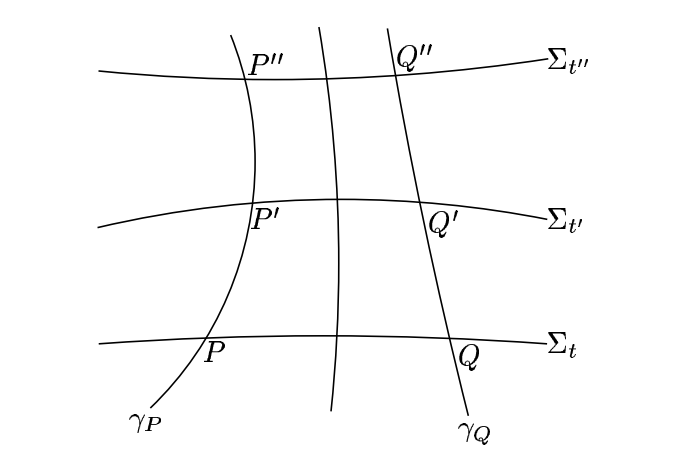
\includegraphics[scale=0.28]{GR/Foliation1.png}
\caption{Foliation of space-time}
\label{fig:side:a}
\end{minipage}%
\begin{minipage}[t]{0.5\linewidth}
\centering
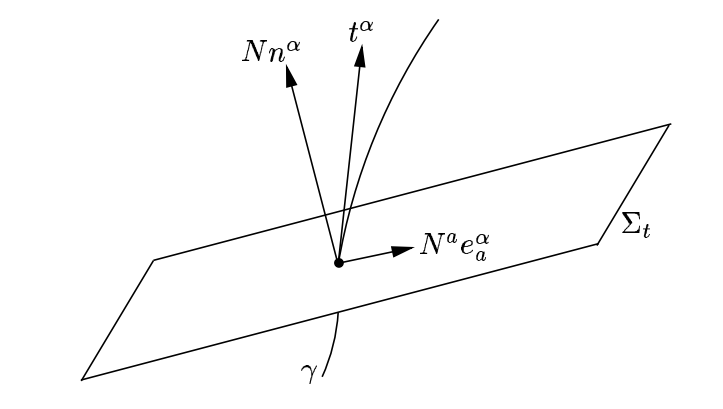
\includegraphics[scale=0.3]{GR/Foliation2.png}
\caption{Decomposition of $t^{\alpha}$}
\label{fig:side:b}
\end{minipage}
\end{figure}
\noindent
The space-time is foliated by spacelike hypersurfaces $\Sigma_t$ that is described by scalar function $t(x^{\alpha})$. $t$ is a single valued function and the unit normal to the hypersurfaces $n_{\alpha} \propto \partial_{\alpha} t$ is a future directed timelike vector field.
\\ \\
Consider a congruence of curves $\gamma$ intersecting $\Sigma_t$. We use $t$ as a parameter on the curves and the vector $t^{\alpha}$ is tangent to the congruence (so, $t^{\alpha} \partial_{\alpha}t = 1$).Install coordinates $y^a$ on $\Sigma_t$ and impose $y^a(P'') = y^a(P') = y^a(P)$, so $y^a$ is held constant on each member of the congruence. This construction defines a coordinate system $(t,y^a)$ in $\mathcal{V}$.\\
\subsubsection{base vector}
\[t^{\alpha} = \left( \frac{\partial x^{\alpha}}{\partial t}\right)_{y^a}, \ \ \ \ e_a^{\alpha} = \left(\frac{\partial x^{\alpha}}{\partial y^a} \right)_t, \ \ \ \ \mathcal{L}_t e_a^{\alpha} = 0.\]
\subsubsection{Normal vector}
\[n_{\alpha} = -N \partial_{\alpha}t, \ \ \ \ n_{\alpha} e_a^{\alpha} = 0.\]
\subsubsection{Decomposition of $t^{\alpha}$}
\[t^{\alpha} = N n^{\alpha} + N^a e_a^{\alpha}.\]
\subsubsection{Metric}
\begin{eqnarray}
ds^2 &=& g_{\alpha \beta} dx^{\alpha} dx^{\beta} \nonumber \\
&=& g_{\alpha \beta} (t^{\alpha} dt + e_a^{\alpha}dy^a) (t^{\beta} dt + e_b^{\beta}dy^{b}) \nonumber \\
&=& -N^2 dt^2 + h_{ab}(dy^a+N^a dt)(dy^b + N^b dt). \nonumber \\
\sqrt{-g} &=& N \sqrt{h}. \nonumber
\end{eqnarray}

\subsection{Field theory}
\[\dot{q} = \frac{\partial q}{\partial t}, \ \ \ \ p=\frac{\partial}{\partial \dot{q}}(\sqrt{-g} \mathcal{L}).\]
\[\mathcal{H}(p,q,q_a) = p\dot{q} - \sqrt{-g} \mathcal{L}.\]
\[H = \int_{\Sigma_t} \mathcal{H}(p,q,q_{,a})d^3y.\]
\[S = \int_{t_1}^{t_2} dt \int_{\Sigma_t} (p \dot{q} - \mathcal{H} ) d^3 y.\]
\[\delta S = 0 \Rightarrow \dot{p} = -\frac{\partial \mathcal{H}}{\partial q} + \left(\frac{\partial \mathcal{H}}{\partial q_{,a}}\right)_{,a}, \ \ \ \ \dot{q} = \frac{\partial \mathcal{H}}{\partial p}.\]
\begin{example}
For electromagnetic field in 3+1 decomposition form, we define the electrical field by $E_a = F_{\alpha \beta} n^{\beta} e_a^{\alpha}$, the magnetic field by $\epsilon_{abc} B^c = F_{\alpha \beta} e_a^{\alpha} e_b^{\beta}$. 
In this definition, the equation of motion of particles in electromagnetic field can be written as
\[m A_a = \gamma e [NE_a + \epsilon_{abc} (v^b+N^b) B^c].\]
where $A_a \equiv u_{\alpha;\beta} u^{\beta} e_a^{\alpha}$, $u^{\nu} = \gamma [Nn^{\nu} + (v^b + N^b) e_{b}^{\nu}]$, and $\gamma \equiv [N^2-(N^b+v^b)(N_b+v_b)]^{-1/2}$.
If we adopt the coordinates $(t,y^a)$, it is easy to verify that
\[E^a = N F^{0a}, \ \ \ \ B^a = \frac{1}{2} \epsilon^{abc} F_{bc}.\]
We further define
\[\mathcal{E}^a = \sqrt{h} E^a, \ \ \ \ \mathcal{B}^a = \sqrt{h} B^a, \ \ \ \ \phi = - A_0, \ \ \ \ \rho_{e} = -j^{\alpha} n_{\alpha} = N j^0.\]
If we notice that
\[F_{0a} = -h_{ab}N^2F^{0b} - F_{ab}N^b, \ \ \ \ \tilde{\epsilon}_{abc} \tilde{\epsilon}_{ijk} h^{ai} h^{bj} = \frac{2h_{ck}}{h}.\]
It is easy to verify that
\[ \sqrt{-g} \mathcal{L} = - \mathcal{E}^a \dot{A_a} + \phi \mathcal{E}^a_{,a} - \frac{1}{2} N h^{-\frac{1}{2}} h_{ab} (\mathcal{E}^a \mathcal{E}^b + \mathcal{B}^a \mathcal{B}^b) + \tilde{\epsilon}_{abc}N^a \mathcal{E}^b \mathcal{B}^c -\sqrt{h} \phi \rho_e + N \sqrt{h} A_a j^a.\]
Therefore, $\pi^a = -\mathcal{E}^a$, and we can get the Hamilton density
\[\mathcal{H} = \phi \pi^a_{,a} + \frac{1}{2} N h^{-\frac{1}{2}} h_{ab} (\pi^a \pi^b + \mathcal{B}^a \mathcal{B}^b) + \tilde{\epsilon}_{abc}N^a \pi^b \mathcal{B}^c +\sqrt{h} \phi \rho_e - N \sqrt{h} A_a j^a.\]
Then, the Hamilton equation can be written as
\[\dot{A}_a = -\phi_{,a} + N h^{-\frac{1}{2}} h_{ab}\pi^b + \tilde{\epsilon}_{abc}N^a \mathcal{B}^c;\]
\[\dot{\pi}^a = - \tilde{\epsilon}^{jab}(Nh^{-\frac{1}{2}}h_{ij}\mathcal{B}^i)_{,b} - \tilde{\epsilon}^{cab}(\tilde{\epsilon}_{ijc}N^i \pi^j)_{,b} + N\sqrt{h}j^a .\]
and also the constraint equation $\pi^a_{,a} + \sqrt{h}\rho_e = 0$.
After simplification, the Maxwell equations are
\begin{eqnarray}
\frac{1}{\sqrt{h}}\frac{\partial}{\partial t}(\sqrt{h} \bm{E}) &=& \nabla \times (N \bm{B} - \bm{N} \times \bm{E}) - N \bm{J}; \nonumber \\
\frac{1}{\sqrt{h}}\frac{\partial}{\partial t}(\sqrt{h} \bm{B}) &=& -\nabla \times (N \bm{E} + \bm{N} \times \bm{B}) ;\nonumber \\
\nabla \cdot \bm{E} &=& \rho_e ;\nonumber \\
\nabla \cdot \bm{B} &=& 0. \nonumber
\end{eqnarray}
\end{example}


\subsection{General relativity}
\[S_G = \frac{1}{16 \pi} \int_{t_1}^{t_2} dt \left\{ \int_{\Sigma_t} \left(\tensor[^3]{R}{} + K^{ab}K_{ab} -K^2 \right) N \sqrt{h} d^3 y + 2\oint_{\Sigma_t}(k-k_0)N \sqrt{\sigma}d^2 \theta \right\} ,\]
where $k_0 =$ extrinsic curvature of $S_t$ embedded in flat space. 

\subsubsection{Gravitational Hamiltonian}
\[\dot{h}_{ab} \equiv \mathcal{L}_t h_{ab} = \mathcal{L}_t (g_{\alpha \beta} e_a^{\alpha} e_b^{\beta}) =  2NK_{ab} + N_{a|b} + N_{b|a}).\]
\[K_{ab} = \frac{1}{2N} (\dot{h}_{ab} - N_{a|b} - N_{b|a}).\]
\[p^{ab} = \frac{\partial}{\partial \dot{h}_{ab}} (\sqrt{-g} \mathcal{L}_G) = \frac{\sqrt{h}}{16\pi} (K^{ab} - K h^{ab}).\]
\[\sqrt{h}K^{ab} = 16\pi (p^{ab} - \frac{1}{2}ph^{ab}).\]
\[\mathcal{H}_G = p^{ab}\dot{h}_{ab} - \sqrt{-g} \mathcal{L}_G.\]
\begin{eqnarray}
16\pi H_G &=& \int_{\Sigma_t} \left[ N(K^{ab}K_{ab} - K^2 - \tensor[^3]{R}{}) - 2N_a(K^{ab} - Kh^{ab})_{|b} \right] \sqrt{h} d^3 y 
\nonumber \\
&\phantom{=}& -2\oint_{S_t} \left[ N(k-k_0) - N_a(K^{ab}-Kh^{ab})r_b \right] \sqrt{\sigma} d^2 \theta .\nonumber
\end{eqnarray}

\subsubsection{Variation of gravitational Hamiltonian}
\[\delta N = \delta N^a = \delta h_{ab} = 0 \mbox{ on } S_t,\]
\[\delta H_G = \int_{\Sigma_t} (\mathcal{P}^{ab} \delta h_{ab} + \mathcal{H}_{ab} \delta p^{ab} - \mathcal{C}\delta N - 2\mathcal{C}_a \delta N^a) d^3 y.\]
\begin{eqnarray}
(16\pi)\mathcal{P}^{ab} &=&  N\sqrt{h}G^{ab} - \sqrt{h}(N^{|ab} - h^{ab} N^{|c}_{\phantom{|c}c}) \nonumber \\
&\phantom{=}& +(16\pi)[2p^{c(a}N^{b)}_{\phantom{b)}|c} - \sqrt{h}(\frac{1}{\sqrt{h}}p^{ab}N^c)_{|c}] \nonumber \\
&\phantom{=}& + (16\pi)^2 [\frac{2N}{\sqrt{h}} (p^a_c p^{bc} - \frac{1}{2} p p^{ab}) - \frac{N}{2\sqrt{h}}(p^{cd}p_{cd} - \frac{1}{2} p^2)h^{ab}]. \nonumber \\
\mathcal{H}_{ab} &=& (16\pi) \frac{2N}{\sqrt{h}} (p_{ab} - \frac{1}{2}p h_{ab}) + 2N_{(a|b)} .\nonumber \\
\mathcal{C} &=& \frac{\sqrt{h}}{16\pi} (\tensor[^3]{R}{} + K^2 - K^{ab}K_{ab}) .\nonumber \\
\mathcal{C}^a &=& \frac{\sqrt{h}}{16\pi} (K_a^{\phantom{a}b} - K \delta_a^{\phantom{a}b})_{|b}. \nonumber 
\end{eqnarray}

\subsubsection{Variation of electromagnetic Hamiltonian}
\[\delta H_E = \int_{\Sigma_t}(-\frac{1}{2}N\sqrt{h}\mathcal{I}^{ab} \delta h_{ab} + \sqrt{h} \rho \delta N - \sqrt{h} s_a \delta N^a).\]
\begin{eqnarray}
\mathcal{I}^{ab} &=& \frac{1}{2}(E^c E_c + B^c B_c)h^{ab} - E^a E^b - B^a B^b. \nonumber \\
\rho &=& \frac{1}{2}(E^c E_c + B^c B_c) .\nonumber \\
s_a &=& \epsilon_{abc} E^b B^c .\nonumber
\end{eqnarray}

\subsubsection{Hamilton's equations}
\[\dot{h}_{ab} = \mathcal{H}_{ab}, \ \ \ \ \dot{p}^{ab} = -\mathcal{P}^{ab}+\frac{1}{2}N\sqrt{h}\mathcal{I}^{ab}.\]
\[\tensor[^3]{R}{} + K^2 - K^{ab}K_{ab} = 16 \pi \rho.\]
\[(K_a^{\phantom{a}b} - K \delta_a^{\phantom{a}b})_{|b} = -8\pi s_a.\]

\chapter{Perturbation Theory and Gravitational Radiation}
\section{The linearized theory of gravity}
In a weak-field situation
\[g_{\mu\nu} = \eta_{\mu\nu} + h_{\mu\nu} , \quad |h_{\mu\nu}| \ll 1 ,\]
one can expand the field equations in powers of $h_{\mu\nu}$ using a coordinate frame where $|h_{\mu\nu}| \ll 1$ holds; and without much loss of accuracy, one can keep only linear terms. The resulting formalism is often called ``the linearized theory of gravity''. The resulting connection coefficients, when linearized in the metric perturbation $h_{\mu\nu}$, read 
\[\Gamma^{\mu}_{\alpha \beta} = \frac{1}{2}\eta^{\mu\nu} [h_{\alpha\nu,\beta} + (h_{\beta\nu,\alpha} - h_{\alpha\beta,\nu})] \equiv \frac{1}{2}(h_{\alpha \phantom{*},\beta}^{\phantom{*} \mu} + h_{\beta \phantom{*},\alpha}^{\phantom{*} \mu} + h_{\alpha\beta}^{\phantom{**} ,\mu} ).\]
Whenever one expands in powers of $h_{\mu\nu}$, indices of $h_{\mu\nu}$ are raised and lowered using $\eta^{\mu\nu}$ and $\eta_{\mu\nu}$, not $g^{\mu\nu}$ and $g_{\mu\nu}$. A similar linearization of the Ricci tensor yields
\[R_{\mu\nu} = \Gamma^{\alpha}_{\phantom{*}\mu\nu,\alpha} - \Gamma^{\alpha}_{\phantom{*}\mu\alpha,\nu} = \frac{1}{2}(h_{\mu \phantom{*},\nu\alpha}^{\phantom{*} \alpha} + h_{\nu \phantom{*},\mu\alpha}^{\phantom{*} \alpha} - h_{\mu\nu,\alpha}^{\phantom{***}\alpha} - h_{,\mu\nu}),\]
where
\[h \equiv \eta_{\mu\nu}h^{\mu\nu}.\]
After a further contraction to form $R \equiv g^{\mu\nu}R_{\mu\nu} \approx \eta^{\mu\nu}R_{\mu\nu}$,
one finds the Einstein equations read
\[h_{\mu\alpha,\nu}^{\phantom{****}\alpha} + h_{\nu\alpha,\mu}^{\phantom{****}\alpha} - h_{\mu\nu,\alpha}^{\phantom{****}\alpha} - h_{,\mu\nu} - \eta_{\mu\nu}(h^{\alpha\beta}_{\phantom{**},\alpha\beta} - h_{,\alpha}^{\phantom{*}\alpha}) = 16\pi T_{\mu\nu}.\]
Define
\[\overline{h}_{\mu\nu} \equiv h_{\mu\nu} - \frac{1}{2}\eta_{\mu\nu}h.\]
The linearized field equations become
\[H^{\mu\alpha\nu\beta}_{\phantom{****},\alpha\beta} = 16\pi T_{\mu\nu},\]
where
\[-H^{\mu\alpha\nu\beta} \equiv \overline{h}^{\mu\nu}\eta^{\alpha\beta} + \overline{h}^{\alpha\beta}\eta^{\mu\nu} - \overline{h}^{\alpha\nu}\eta^{\mu\beta} - \overline{h}^{\mu\beta}\eta^{\alpha\nu} .\]
\\
Two different types of coordinate transformations connect nearly globally Lorentz systems to each other: global Lorentz transformations, and infinitesimal coordinate
transformations.
\\ \\
Global Lorentz Transformations:
\\
\[x^{\mu} = \Lambda^{\mu}_{\phantom{*}\alpha'}x^{\alpha'} , \quad \Lambda^{\mu}_{\phantom{*}\alpha'} \Lambda^{\nu}_{\phantom{*}\beta'} \eta_{\mu\nu} = \eta_{\alpha'\beta'} .\]
We can verify that $h_{\mu\nu}$ and $\bar{h}_{\mu\nu}$
transform like components of a tensor in flat spacetime
\[h_{\alpha'\beta'} = \Lambda^{\mu}_{\phantom{*}\alpha'} \Lambda^{\nu}_{\phantom{*}\beta'} h_{\mu\nu}.\]
Infinitesimal Coordinate Transformations:
\\
\[x^{\mu'} = x^{\mu} + \xi^{\mu},\]
where $\xi^{\mu}$ are four arbitrary functions small enough to leave $|h_{\mu'\nu'}| \ll 1$. We can verify that the metric perturbation functions in the new $x^{\mu'}$ and old $x^{\mu}$ coordinate systems are related by
\[h_{\mu\nu}^{\mathrm{new}} = h_{\mu\nu}^{\mathrm{old}} - \xi_{\mu,\nu} - \xi_{\nu,\mu},\]
whereas the functional forms of all other scalars, vectors, and tensors which is of order $O(h)$, such as $R_{\mu\nu}$, $T_{\mu\nu}$ and $R$, are unaltered, to within the precision of linearized theory. 
\\ \\
For any physical situation, one can specialize the gauge so that
\[\overline{h}^{\mu\alpha}_{\phantom{**},\alpha} = 0,\] 
called Lorentz gauge. 
The Lorentz gauge is not fixed uniquely. The gauge condition is left unaffected by any gauge transformation for which
\[\Box \xi \equiv \xi^{\alpha,\beta}_{\phantom{**}\beta} = 0.\]
The field equations then become
\[\Box \overline{h}_{\mu\nu} = -16\pi T_{\mu\nu}.\]
Once the gauge has been fixed by fiat for a given system, one can regard $h_{\mu\nu}$ as components of tensors in flat spacetime; and one can regard the field equations and the chosen gauge conditions as geometric, coordinate-independent equations in flat spacetime.
This viewpoint allows one to use curvilinear coordinates, if one wishes. But in doing so, one must everywhere replace the Lorentz components of the metric $\eta_{\mu\nu}$ by the metric's components $g_{\mu\nu_{\mathrm{flat}}}$ in the flat-spacetime curvilinear coordinate system; and one must replace all ordinary derivatives in the field equations and gauge conditions by covariant derivatives whose connection coefficients come from $g_{\mu\nu_{\mathrm{flat}}}$.

\section{Nearly Newtonian gravitational fields}
The general solution to the linearized field equations in Lorentz gauge lends itself to expression as a retarded integral of the form familiar from electromagnetic theory:
\[\overline{h}_{\mu\nu}(t,\bm{x}) = \int \frac{4T_{\mu\nu}(t-r,\bm{x}')}{r} d^3x' , \quad r = |\bm{x}-\bm{x}'|.\]
Here focus attention on a nearly Newtonian source: $T_{00} \gg |T_{0i}|$ and $T_{00} \gg |T_{ij}|$, and velocities
slow enough that retardation is negligible. In this case, we have
\[\overline{h}_{00} = -4\Phi , \quad \overline{h}_{0i} = \overline{h}_{ij} = 0.\]
\[\Phi(t,\bm{x}) = -\int \frac{T_{00}(t,\bm{x}')}{r} d^3x' = \mbox{ Newtonian potential }.\]
The corresponding metric is
\[ds^2 = -(1+2\Phi)dt^2 + (1-2\Phi)(dx^2 + dy^2 + dz^2) \approx -(1-\frac{2M}{r})dt^2 + (1+\frac{2M}{r})(dx^2 + dy^2 + dz^2).\]
For a test particle whose velocity $v \ll 1$, the geodesic equation can be written as
\[\frac{d^2 v^i}{dt^2} + \Gamma^{i}_{00} = \frac{d^2 v^i}{dt^2} + \Phi_{,i} = 0.\]
Therefore, we reproduce the classical Newtonian gravitation theory.
\\ \\
Now let us consider the path of a photon through
this geometry; in other words, solve the perturbed geodesic equation for a null trajectory $x^{\mu}(\lambda)$. (We parametrize the trajectory with $\lambda$ to ensure that $p^{\mu} = dx^{\mu}/d\lambda$.)
Recall that our philosophy is to consider the metric perturbation as a field defined on a flat background spacetime. 
Similarly, we can decompose the geodesic into a background path plus a perturbation,
\[x^{\mu}(\lambda) = x^{(0)\mu}(\lambda) + x^{(1)\mu}(\lambda),\]
where $x^{(0)\mu}(\lambda)$ solves the geodesic equation in the background. 
We then evaluate all quantities along the background path, to solve for $x^{(1)\mu}(\lambda)$. 
For this procedure to make sense, we need to assume that the potential $\Phi$ is not appreciably different along the background and true geodesies;
this condition amounts to requiring that $x^{(1)i}\partial_{i}\Phi \ll \Phi$. 
For convenience we denote the wave vector of the background path as $k^{\mu}$ and the derivative of the deviation vector as $l^{\mu}$. The condition that a path be null is of course
\[(\eta_{\mu\nu} + h_{\mu\nu})(l^{\mu}+k^{\mu})(l^{\nu} + k^{\nu}) = 0.\]
At zeroth order we simply have
\[\eta_{\mu\nu} k^{\mu} k^{\nu} = 0.\]
i.e.
\[k^2 \equiv (k^0)^2 = \vec{k}\cdot\vec{k}.\]
At first order we obtain
\[2\eta_{\mu\nu}k^{\mu}l^{\nu} + h_{\mu\nu}k^{\mu}k^{\nu} = 0,\]
i.e.
\[-k l^0 + \vec{l}\cdot\vec{k} = 2k^2\Phi.\]
We now turn to the perturbed geodesic equation. The zeroth-order geodesic equation simply tells us that $x^{(0)\mu}(\lambda)$ is a straight  trajectory, while at first order we have
\[\frac{dl^{\mu}}{d\lambda} = -\Gamma^{\mu}_{\rho\sigma}k^{\rho}k^{\sigma},\]
i.e.
\[\frac{dl^0}{d\lambda} = -2k(\vec{k}\cdot\vec{\nabla}\Phi), \quad \frac{d\vec{l}}{d\lambda} = -2k^2\vec{\nabla}_{\bot}\Phi,\]
where $\vec{\nabla}_{\bot} \equiv \vec{\nabla} - k^{-2}(\vec{k}\cdot\vec{\nabla})\vec{k}$.
Putting all equations together, we have
\[l^0 = -2k \Phi, \quad \vec{l} \cdot \vec{k} = 0, \quad \vec{l} = -2k^2 \int \vec{\nabla}_{\bot}\Phi d\lambda.\] 
The redshift due to gravitation is
\[z \equiv \frac{l^0}{k} = -2\Phi.\]
The deflection angle due to gravitation is
\[\vec{\alpha} = -\frac{\vec{l}}{k} = 2k\int \vec{\nabla}_{\bot}\Phi d\lambda.\]
Particularly, if $\Phi = -M/r$, we can get
\[z = \frac{2M}{r}, \quad \alpha = \frac{4M}{b},\]
where $b$ is the distance between mass point and light ray.

\section{Gravitational wave}
Let us decompose $h_{\mu\nu}$ as
\[h_{00} = -2A , \quad h_{0i} = \partial_i B + \bar{B}_i , \quad h_{ij} = 2C\delta_{ij} + 2\partial_i\partial_j E + \partial _i\bar{E}_j + \partial_j\bar{E}_i + \tilde{E}_{ij} \]
with
\[\partial_i \bar{B}_i = 0 , \quad \partial_i \bar{E}_i = 0 , \quad \partial_i \tilde{E}_{ij} = 0 , \quad \tilde{E}^i_i = 0.\]
Then we decompose the displacement vector for gauge transformation as
\[\xi^0 = -T , \quad \xi^i = -\partial^i L - \bar{L}^i \]
with $\partial_i \bar{L}^i = 0$. 
Under such coordinate transformation , the metric transform as
\[A \to A + \dot{T} , \quad B \to B + \dot{L} - T , \quad C \to C , \quad E \to E  + L \]
for the scalar modes,
\[\bar{B}_i \to \bar{B}_i + \dot{\bar{L}}_i , \quad \bar{E}_i \to \bar{E}_i + \bar{L}_i \]
for the vector modes, and the tensor modes remain unchanged
\[\tilde{E}_{ij} \to \tilde{E}_{ij}.\]
The tensor modes are therefore gauge invariant since they do not depend on the choice of the coordinate system. This is not the case for the vector and scalar modes. 
However, we can define a combination of these modes that are gauge invariant. For the scalar modes, we define
\[\Phi = A + \dot{B} - \ddot{E} , \quad \Psi = -C, \]
and for the vector modes
\[\bar{\Psi}_i = \dot{\bar{E}}_i - \bar{B}_i.\]
We therefore have defined 2 scalar quantities and 1 vector quantity (2 degrees of freedom) which are gauge invariant. All together , we therefore have $6$ degrees of freedom, once the $4$ arbitrary degrees of freedom related to the gauge choice have been absorbed.
\\ \\
In terms of gauge invariant quantities, the Einstein tensor can be written as
\begin{eqnarray}
G_{00} &=& 2\nabla^2 \Psi, \nonumber \\
G_{0i} &=& 2\nabla_{i} \dot{\Psi} + \frac{1}{2}\nabla^2 \bar{\Psi}_{i}, \nonumber \\
G_{ij} &=& (\delta_{ij}\nabla^2-\nabla_{i} \nabla_{j})(\Phi-\Psi) + \frac{1}{2}\left( \nabla_{i} \dot{\bar{\Psi}}_{j} + \nabla_{j} \dot{\bar{\Psi}}_{i}\right) + 2\delta_{ij}\ddot{\Psi} - \frac{1}{2}\Box \tilde{E}_{ij}. \nonumber
\end{eqnarray}
Thus we note again that Einstein tensor (Ricci tensor) is gauge invariant.
\\ \\
Now we consider the solution of linearised Einstein equation in vacuum.
For the scalar modes, the Einstein equation $G_{\mu\nu} = 0$ imply that
\[\nabla^2 \Psi = 0 , \quad \nabla^2(\Phi-\Psi) = 0.\]
The only regular solutions are
\[\Phi = \Psi = 0,\]
which means that no scalar mode can propagate.
\\ \\
For the vector modes, we have
\[\nabla^2 \bar{\Psi}_i = 0.\]
The only regular solution is $\bar{\Psi}_i = 0$. Just as for scalar modes, no vector modes can propagate.
\\ \\
For tensor modes, we have
\[\Box \tilde{E}_{ij} = 0.\]
Therefore, the only perturbations that can propagate in a Minkowski space-time are the gravitational waves and they satisfy
\[\Box \tilde{E}_{ij} = 0 , \quad \partial_i \tilde{E}_{ij} = 0 , \quad \tilde{E}^i_i = 0.\]
The three conditions $\Phi = \Psi = \bar{\Psi}_i = 0$ define a gauge equivalence class. We can choose a gauge in this family by imposing some conditions on the perturbations. For instance, setting $E = B = 0$ and $\bar{E}_i = 0$, we define what is called a transverse and traceless (TT) gauge in which the metric is completely determined. In this case, the only non-vanishing component of $h_{\mu\nu}^{\mathrm{TT}}$ is $\tilde{E}_{ij}$.
A particularly useful set of solutions to this wave 
equation are the plane waves, given by
\[h^{\rm TT}_{\mu\nu} = C_{\mu\nu}e^{ik^{\sigma}x_{\sigma}},\]
where $C_{\mu\nu}$ is a constant, symmetric, traceless
and purely spatial tensor. The Einstein equation  now becomes
\[k^{\sigma}k_{\sigma} = 0, \quad k^{\mu} C_{\mu\nu} = 0.\]
Our solution can be made more explicit by choosing spatial coordinates such that the wave is travelling in the $z$ direction. A little algebra can show that
\[h_{ij}^{\rm TT} = \left( C_{+}\epsilon^+_{ij} + C_{\times} \epsilon^{\times}_{ij} \right) e^{-i\omega(t-z)},\]
with the two polarization tensors being defined by
\[\epsilon^+ \equiv \begin{pmatrix}
1 & 0 & 0\\ 0 & -1 & 0 \\ 0 & 0 & 0
\end{pmatrix} , \quad \epsilon_{\times} \equiv \begin{pmatrix}
0 & 1 & 0\\ 1 & 0 & 0 \\ 0 & 0 & 0
\end{pmatrix} .\]
\begin{figure}[!h]
\centering
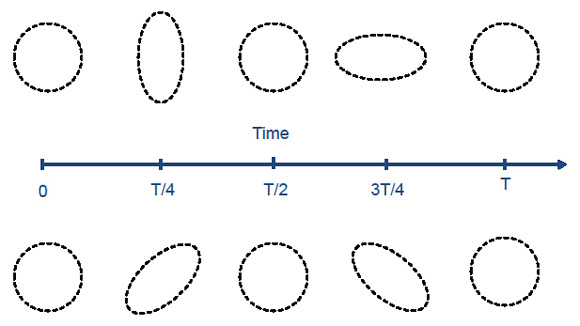
\includegraphics[scale=0.4]{./GR/GW.jpg}
\caption{Effects of a gravitational plane wave propagating along the axis $z$ on a ring of particles located in the plane $xy$, depending on the wave polarization.}
\end{figure}
\noindent
Consider the geodesic equation of a test particle in the gravitational field of a gravitational wave in the TT gauge. Since to leading order in perturbation we have $\Gamma^i_{00} = 0$, a particle initially at rest will remain at rest.
Of course, this does not mean that nothing happens , but rather that the frame of reference is co moving with the test particle. To see if anything happens , we should look at the relative motion of two neighbouring particles, which can be done using the geodesic deviation equation. The relative acceleration is given by
\[\nabla_{\bm{u}} \nabla_{\bm{u}} \bm{n} = -R(\bm{n},\bm{u}) \bm{u}.\]
To leading order in $v$, we have $u^{\mu} = (1,0)$ and $n^{\mu} = (0,n^i)$, $R_{i00j} = \frac{1}{2}\ddot{h}_{ij}^{\mathrm{TT}}$. Thus that
\[\frac{d^2n^i}{dt^2} = \frac{1}{2} \ddot{h}_{ij} ^{\mathrm{TT}} n^j.\]
For $+$ modes, we have
\[\frac{d^2n^x}{dt^2} = - \frac{1}{2}\omega^2 C_{+}n^x e^{-i\omega(t-z)}, \quad \frac{d^2n^y}{dt^2} = \frac{1}{2}\omega^2 C_{+}n^y e^{-i\omega(t-z)}.\]
For $\times$ modes, we have
\[\frac{d^2n^x}{dt^2} = - \frac{1}{2}\omega^2 C_{\times}n^y e^{-i\omega(t-z)}, \quad \frac{d^2n^y}{dt^2} = - \frac{1}{2}\omega^2 C_{\times}n^x e^{-i\omega(t-z)}.\]

\section{Production of gravitational wave}
Define the Fourier transform of metric perturbation, by
\[\widetilde{\bar{h}}_{\mu\nu}(\omega, \bm{x}) \equiv \int dt e^{i\omega t} \bar{h}_{\mu\nu}(t,x).\]
In Lorentz gauge, we have
\[\widetilde{\bar{h}}_{\mu\nu}(\omega, \bm{x}) = 4\int d^3x' e^{i\omega R} \frac{\widetilde{T}_{\mu\nu}(\omega,\bm{x}')}{R},\]
where $R \equiv |\bm{x} - \bm{x}'|$.
We now make the approximations that our source is isolated, far away, and slowly moving. This leaves us with
\[\widetilde{\bar{h}}_{\mu\nu}(\omega, \bm{x}) = \frac{4e^{i\omega r}}{r} \int d^3x' \tilde{T}_{\mu\nu}(\omega, \bm{x}').\]
The Lorenz gauge condition $\partial_{\mu}\bar{h}^{\mu\nu}(t,\bm{x}) = 0$ in Fourier space implies $i\omega \widetilde{\bar{h}}^{0\nu} = \partial_{i} \widetilde{\bar{h}}^{i\nu}$. 
We therefore only need to concern ourselves with the spacelike components of $\widetilde{\bar{h}}$.
We therefore want to take the integral of the spacelike components $\widetilde{T}^{\mu\nu}$. After some simplification, we can get
\[\int d^3y \widetilde{T}^{ij}(\omega,\bm{y}) = - \frac{\omega^2}{2} \int  d^3y \, y^i y^j \widetilde{T}^{00}.\]
It is conventional to define the quadrupole moment tensor of the energy density of the source,
\[I^{ij} \equiv \int d^3y \, T^{00} y^i y^j.\]
Transform back to $t$ and we can obtain the quadrupole formula,
\[\bar{h}_{ij}(t,\bm{x}) = \frac{2}{r} \frac{d^2 I_{ij}}{dt^2}(t-r).\]
One case of special interest is the gravitational radiation emitted by a binary star. 
For simplicity let us consider two stars of mass $M$ in a circular orbit in the $x-y$ plane, at distance $R$ from their common center of mass. 
We will treat the motion of the stars in the Newtonian approximation. The angular frequency of the orbit is $\Omega = (M/4R^3)^{1/2}$. 
The corresponding energy density is
\[T^{00}(t,\bm{x}) = M\delta(z) [\delta(x-R\cos\Omega t)\delta(y-R\sin\Omega) + \delta(x+R\cos\Omega t)\delta(y+R\sin\Omega)].\]
The quadrupole moment in $x-y$ plane if the system is
\[I = MR^2 \begin{pmatrix}
1 + \cos 2\Omega t & \sin 2\Omega t \\
\sin 2\Omega t & 1 - \cos 2\Omega t
\end{pmatrix}. \]
Thus the spacelike metric perturbation in $x-y$ plane is
\[\bar{h} = \frac{8M\Omega^2R^2}{r} \begin{pmatrix}
- \cos 2\Omega (t-r) & -\sin 2\Omega (t-r) \\
-\sin 2\Omega (t-r) & + \cos 2\Omega (t-r)
\end{pmatrix}. \]

\section{External field of a gravitating source}
Consider an isolated system with gravity so weak that in calculating its structure and motion one can completely ignore self-gravitational effects. We can work out the weak gravitational field,
\[\bar{\bar{h}}_{\mu\nu}(t,\bm{x}) \equiv h_{\mu\nu}(t,\bm{x}) = \int \frac{4\bar{T}_{\mu\nu}(t-R,\bm{x}')}{R} d^3x',\]
produced by such a system. Restrict attention to the spacetime region far outside the system, and expand $h_{\mu\nu}$ in powers of $\bm{x}' / {r}$, we can get
\begin{eqnarray}
ds^2 &=& -\left[1-\frac{2M}{r} + O({1}/{r^3}) \right]dt^2 - \left[4\epsilon_{jkl}S^k \frac{x^l}{r^3} + O({1}/{r^3})  \right] dtdx^i  \nonumber \\
&+& \left[(1+\frac{2M}{r})\delta_{jk} + \mbox{ gravitational radiation terms that die out as } O(1/r) \right]dx^j dx^k , \nonumber
\end{eqnarray}
where
\[M \equiv \int T^{00}d^3x , \quad S_k \equiv \int \epsilon_{klm}x^l T^{m0} d^3x .\]
It is plausible to say the mass of the system is $M$ and the angular momentum $\bm{S}$. With an appropriate choice of gauge, $g_{00}$ far from any weak source are time-independent and are determined uniquely by the source's mass $M$; $g_{0j}$ is time-independent and is fixed by the source's intrinsic angular momentum $S^j$; but $g_{jk}$ has time-dependent terms (gravitational waves) of $O(1/r)$.
\\ \\
The values of a system's mass and angular momentum can be measured by probing the imprint they leave in its external gravitational field. 
Of all tools one might use to probe, the simplest is a test particle in a gravitationally bound orbit. 
If the particle is sufficiently far from the source, its motion is affected hardly at all by the source's angular momentum or by the gravitational waves; only the spherical, Newtonian part of the gravitational field has a significant influence. 
Hence, the particle moves in an elliptical Keplerian orbit. To determine the source's mass $M$, one need only apply Kepler's third law
\[M = \left( \frac{2\pi}{\mbox{orbital period}} \right)^2 \left(\mbox{ Semi-major axis of ellipse } \right)^3.\]
Angular momentum can be probed by a gyroscope.
Place a gyroscope at rest in the source's gravitational field.
By a force applied to its center of mass, prevent it from falling. 
As time passes, the $g_{0j}$ term in the metric will force the gyroscope to precess relative to the basis vectors $\partial_{i}$; and since these basis vectors are ``tied'' to the coordinate system, which
in turn is tied to the Lorentz frames at infinity, which in turn are tied to the ``fixed stars'' , the precession is relative to the ``fixed stars.'' 
The angular velocity of precession is
\[\bm{\Omega} = \frac{1}{r^3} \left[ -\bm{S} + \frac{3(\bm{S}\cdot \bm{x})\bm{x}}{r^3} \right] .\]
One sometimes says that the source's rotation ``drags the inertial frames near the source,'' thereby forcing the gyroscope to precess.
\\ \\
Consider an isolated, gravitating system inside which spacetime may or may not be highly curved. We restrict attention to the weak gravitational field far from the source, and analyze it using linearized theory in vacuum.
Expand $h_{\mu\nu}$ in multipole moments and powers of $1/r$; and adjust the gauge, the Lorentz frame, and the origin of coordinates to simplify the resulting metric.
We have
\begin{eqnarray}
ds^2 &=& -\left[1-\frac{2M}{r} + \frac{2M^2}{r^2} + O({1}/{r^3}) \right]dt^2 - \left[4\epsilon_{jkl}S^k \frac{x^l}{r^3} + O({1}/{r^3})  \right] dtdx^i  \nonumber \\
&+& \left[(1+\frac{2M}{r} + \frac{3M^2}{2r^2})\delta_{jk} + \mbox{ gravitational radiation terms that die out as } O({1}/{r}) ) \right]dx^j dx^k. \nonumber
\end{eqnarray}
However, $M$ and $\bm{S}$ is not a simple integration of $T^{00}$ and $\epsilon_{klm} x^l T^{0m}$ of the system as in the case of weakly gravitating sources.
However, since this integration is impossible to measure in practice. We always determine the mass of the star by studying the orbits of planets in its external gravitational field. Therefore, one defines the ``total mass-energy'' $M$ of the sun or other body to be the constant that appears in the line element for its distant external spacetime geometry. Similarly, one defines the body's intrinsic angular momentum as the constant 3-vector $\bm{S}$ appearing in its line element.

\section{Conservation laws for 4-momentum and angular momentum}
Recall in the weak field limit, the Einstein equation can be written as
\[H^{\mu\alpha\nu\beta}_{\phantom{****},\alpha
\beta} = 16\pi T^{\mu\nu}.\]
Thus we have
\[T^{\mu\nu}_{\phantom{**},\nu} = \frac{1}{16\pi}H^{\mu\alpha\nu\beta}_{\phantom{****},\alpha\beta\nu} = 0.\]
The source's total 4-momentum can be defined as
\[P^{\mu} \equiv \int T^{\mu 0}d^3x = \frac{1}{16\pi} \oint_{S} H^{\mu\alpha 0 j}_{\phantom{****},\alpha} d^2 S_j .\]
Particularly, we have
\[P^0 = \frac{1}{16\pi} \oint_{S} (g_{jk,k} - g_{kk,j})d^2S_{j} .\]
The angular momentum of the source can be defined as
\[J^{\mu\nu} \equiv \int (x^{\mu} T^{0\nu} - x^{\nu} T^{0\mu}) d^3x  = \frac{1}{16\pi} \oint_S (x^{\mu}H^{\nu\alpha 0 j}_{\phantom{****},\alpha} - x^{\nu}H^{\mu\alpha 0 j}_{\phantom{****},\alpha} + H^{\mu j 0 \nu} - H^{\nu j 0 \nu}) d^2 S_j .\]
\begin{note}
To evaluate the flux integrals (by contrast with the volume
integrals), one need utilize only the gravitational field far outside the source. Since that gravitational field has the same form in full general relativity for strong sources as in linearized theory for weak sources, the flux integrals can be used to figure out $P^{\mu}$ and $J^{\mu\nu}$ for any isolated source whatsoever, weak or strong. Thus we will use the flux integrals as the definition.
\end{note}

\noindent
Knowing $P^{\mu}$ and $J^{\mu\nu}$, one can figure out the source's total mass-energy $M$ intrinsic angular momentum $S_{\rho}$ by
\[M = (-P^{\mu}P_{\mu})^{-1/2};\]
\[Y^{\mu} = -J^{\mu\nu}P_{\nu}/M^2;\]
\[S_{\rho} = \frac{1}{2}\epsilon_{\mu\nu\sigma\rho}(J^{\mu\nu} - Y^{\mu}P^{\nu} + Y^{\nu}P^{\mu})P^{\sigma}/M.\]
Note especially that the integrands of the flux integrals  are not gauge-invariant. In any local inertial frame at an event they vanish. 
However, the total integrals $P^{\mu}$ and $J^{\mu\nu}$ are. 
They have meaning and significance independent of any coordinate system and gauge. They are tensors in the asymptotically flat region surrounding the source.
\\ \\
In full general relativity, though $|h_{\mu\nu}| \ll 1$ breaks down, we can still define formally
\[-H^{\mu\alpha\nu\beta} \equiv \overline{h}^{\mu\nu}\eta^{\alpha\beta} + \overline{h}^{\alpha\beta}\eta^{\mu\nu} - \overline{h}^{\alpha\nu}\eta^{\mu\beta} - \overline{h}^{\mu\beta}\eta^{\alpha\nu} , \quad h_{\mu\nu} \equiv g_{\mu\nu} - \eta_{\mu\nu}.\]
And we define the effective energy-momentum pseudotensor by
\[H^{\mu\alpha\nu\beta}_{\phantom{****},\alpha
\beta} = 16\pi T^{\mu\nu}_{\mathrm{eff}}.\]
Therefore, we have
\[T^{\mu\nu}_{\mathrm{eff},\nu} = 0.\]
\[P^{\mu} = \frac{1}{16\pi} \int d^3x T^{\mu0}_{\mathrm{eff}};\]
\[J^{\mu\nu} = \int (x^{\mu} T^{0\nu}_{\mathrm{eff}} - x^{\nu} T^{0\mu}_{\mathrm{eff}}) d^3x.\]
for both strong or weak source.
Define gravitation energy-momentum pseudotensor as
\[16\pi t^{\mu\nu} \equiv H^{\mu\alpha\nu\beta}_{\phantom{****},\alpha
\beta} - 2G^{\mu\nu},\]
so we have $T^{\mu\nu}_{\mathrm{eff}} = T^{\mu\nu} + t^{\mu\nu}$. 
All the quantities $H^{\alpha\mu\nu\beta}$, $t^{\mu\nu}$ and $T^{\mu\nu}_{\mathrm{eff}}$ depend for their definition and existence on the choice of coordinates.
There is, nevertheless, adequate invariance under general coordinate transformations to give the values $P^{\mu}$ and $J^{\mu\nu}$ of the volume integrals geometric, coordinate-free significance in the asymptotically flat region far outside the source.
Although this invariance is hard to see in the volume integrals themselves, it is clear from the surface-integral forms that no coordinate transformation which changes the coordinates only inside some spatially bounded region can influence the values of the integrals. 
For coordinate changes in the distant, asymptotically
flat regions, linearized theory guarantees that under Lorentz transformations the integrals for $P^{\mu}$ and $J^{\mu\nu}$ will transform like special relativistic tensors, and that under infinitesimal coordinate transformations (gauge changes) they will be invariant.
\\ \\
It is clear that any quantities $H^{\alpha\mu\nu\beta}_{\mathrm{new}}$  which agree with the original $H^{\alpha\mu\nu\beta}$ in the asymptotic weak-field region will give the same values as $H^{\alpha\mu\nu\beta}$ does for the $P^{\mu}$ and $J^{\mu\nu}$ surface integrals. One especially convenient
choice is Landau-Lifshitz pseudotensor. The details can be found in section 96 of \emph{The Classical Theory of Fields (L.D.Landau \& E.M.Lifshitz)}.
For a system of gravitating bodies, we have
\[\frac{dP^{\mu}}{dt} = -\oint T^{\mu j}_{\mathrm{eff}}d^2S_j ;\]
\[\frac{dJ^{\mu\nu}}{dt} = -\oint(x^{\mu}T^{\nu j}_{\mathrm{eff}} - x^{\nu}T^{\mu j}_{\mathrm{eff}}) d^2 S_j.\]
The flux is integrated over the surface in asymptomatic flat region. Although the pseudotensor $t^{\mu\nu}$ in the interbody region and outside the system, contributes negligibly to the total 4-momentum and angular momentum, its contribution via gravitational waves to the time derivatives can be important when added up over astronomical periods of time. Thus, one must not ignore it in the flux integrals.
\\ \\
There are some limitations on our interpretation of $t_{\mu\nu}$ as an energy-momentum tensor. 
It is not invariant  under gauge transformations. 
One way of circumventing this difficulty is to average the energy-momentum tensor over several wavelengths, an operation we denote by angle brackets $\langle \cdots \rangle$.
Since any terms that are derivatives (as opposed to products of derivatives) will average to zero, we are therefore empowered to integrate by parts under the averaging brackets,
\[\langle A(\partial_{\mu} B) \rangle = - \langle (\partial_{\mu} A)B \rangle.\]
After a lot of messy intermediate steps, we will arrive at
\[t_{\mu\nu} = \frac{1}{32\pi} \left\langle (\partial_{\mu}h_{\rho\sigma})(\partial_{\nu}h^{\rho\sigma}) - \frac{1}{2} \partial_{\mu} h \partial_{\nu} h - (\partial_{\rho}h^{\rho\sigma})(\partial_{\mu}h_{\nu\sigma}) - (\partial_{\rho}h^{\rho\sigma})(\partial_{\nu}h_{\mu\sigma})\right\rangle + O(h^3).\]
Since we only care about $t_{\mu\nu}$ in vacuum far from the source, we can adopt TT gauge and neglect higher order terms. 
For a ``monochromatic'' plane gravitational wave $h^{\rm TT}_{\mu\nu} = C_{\mu\nu} \sin(k^{\sigma}x_{\sigma})$, the energy- momentum tensor is
\[t_{\mu\nu} = \frac{1}{64\pi} k_{\mu}k_{\nu} {\rm Tr}(C^2).\]
It the wave is propagating along $z$ direction, we have
\[t^{\mu\nu} = \frac{\pi}{8G} f^2(C_{+}^2 + C_{\times}^2) \begin{pmatrix}
1 & 0 & 0 & 1 \\
0 & 0 & 0 & 0 \\
0 & 0 & 0 & 0 \\
1 & 0 & 0 & 1 
\end{pmatrix}, \]
where $f = \omega / 2\pi$ is the frequency of gravitational wave.
We now can use our formula for the gravitational-wave energy-momentum tensor to calculate the rate of energy loss from a system emitting gravitational radiation
according to the quadrupole formula. We omit the derivation here and write down the final expression directly,
\[P = -\frac{1}{5}\left\langle \frac{d^3 J_{ij}}{dt^3} \frac{d^3 J^{ij}}{dt^3}  \right\rangle,  \]
where $J_{ij} \equiv I_{ij} - 1/3 \delta_{ij} {\rm Tr}I$, called reduced quadrupole moment. The power of gravitational wave generated by binary stars is
\[P = \frac{2}{5} \frac{M^5}{R^5}.\]

\chapter{Black Holes}
\section{Schwarzschild black hole}
\subsection{Schwarzschild metric}
In spherical coordinates $\{t,r,\theta,\phi\}$, the metric is given by
\[ds^2 = -\left(1 - \frac{2M}{r} \right)dt^2 + \left(1 - \frac{2M}{r} \right)^{-1}dr^2 + r^2 d\Omega^2,\]
where $d\Omega^2$ is the metric on a unit two-sphere,
\[d\Omega^2 = d\theta^2 + \sin^2\theta d\phi^2.\]

\begin{newthem}[Birkhoff's theorem]
Schwarzschild metric is the unique vacuum solution with spherical symmetry.
\end{newthem}
\noindent
The proof can be found in section 5.2 of \emph{Spacetime and Geometry (Sean Carroll)}. 
Any spherically symmetric vacuum metric possesses a timelike Killing vector. A metric that possesses a Killing vector that is timelike near infinity is called stationary. A metric is called static if it possesses a timelike Killing vector that is orthogonal to a family of hypersurfaces. 
An alternative definition of ``static'' is stationary, and invariant under time reversal. We should think of stationary as meaning ``doing exactly the same thing at every time,'' while static means ``not doing anything at all.''
\\ \\
The Schwarzschild metric coefficients become infinite at $r = 0$ and $r = 2M$. 
The metric coefficients are coordinate-dependent quantities, it is certainly possible to have a coordinate singularity that results from a breakdown of a specific coordinate system rather than the underlying manifold. 
Direct calculation reveals that
\[R^{\mu\nu\rho\sigma}R_{\mu\nu\rho\sigma} = \frac{48M^2}{r^6}.\]
This is enough to convince us that $r = 0$ represents an honest singularity.
\\ \\
As for $r = 2M$, the Schwarzschild radius. We can check that none of the curvature invariants blows up there. We therefore begin to think that it is actually not singular, and we have simply chosen a bad coordinate system. The surface $r = 2M$ is very well-behaved in the Schwarzschild metric -- it demarcates the event horizon of a black hole.

\subsection{Geodesics of Schwarzschild spacetime}
There are four Killing vectors in Schwarzschild Space-time: three for the spherical symmetry, and one for time translations.
Each of these will lead to a constant of the motion for a free particle.
If $K_{\mu}$ is a Killing vector, we know that
\[K_{\mu} \frac{dx^{\mu}}{d\lambda} \]
is a constant along the geodesic.
Here, we choose the affine parameter $\lambda$ of geodesics to make $dx^{\mu}/d\lambda$ four velocity for massive particles and four momentum for massless particles. Thus the quantity
\[\epsilon = -g_{\mu\nu} \frac{dx^{\mu}}{d\lambda} \frac{dx^{\mu}}{d\lambda}\]
is constant along the path. For massive particles $\epsilon = 1$ while for massless particles, $\epsilon = 0$.
\\ \\
We can think of the angular momentum as a three-vector with a magnitude (one component) and direction (two components). 
Conservation of the direction of angular momentum means that the particle will move in a plane. We can choose this to be the equatorial plane of our coordinate system. Thus, the two Killing vectors that lead to conservation of the direction of angular momentum imply that, for a single particle, we can choose
\[\theta = \frac{\pi}{2}.\]
The two remaining Killing vectors correspond to energy and the magnitude of angular momentum. The energy arises from the timelike Killing vector
\[K^{\mu} = (\partial_t)^{\mu} = (1,0,0,0), \; K_{\mu} = (\frac{2M}{r}-1, 0,0,0)\]
The Killing vector whose conserved quantity is the magnitude of the angular momentum is
\[R^{\mu} = (\partial_{\phi})^{\mu} = (0,0,0,1), \; R_{\mu} = (0,0,0,r^2\sin^2\theta) \]
The two conserved quantities are
\[E = -K_{\mu} \frac{dx^{\mu}}{d\lambda} = \left( 1- \frac{2M}{r}\right) \frac{dt}{d\lambda}, \; L = R_{\mu} \frac{dx^{\mu}}{d\lambda} = r^2\frac{d\phi}{d\lambda}\]
For massless particles, these can be thought of as the conserved energy and angular momentum, while for massive particles they are the conserved energy and angular momentum per unit mass of the particle.
\\ \\
After some algebra manipulations, we can get a single equation for $r(\lambda)$,
\[\frac{1}{2} \left( \frac{dr}{d\lambda} \right)^2 + V(r) = \mathcal{E},\]
where
\[V(r) = \frac{1}{2}\epsilon - \epsilon \frac{M}{r} + \frac{L^2}{2r^2} - \frac{ML^2}{r^3}\]
and
\[\mathcal{E} = \frac{1}{2}E^2.\]

\begin{figure}
\centering
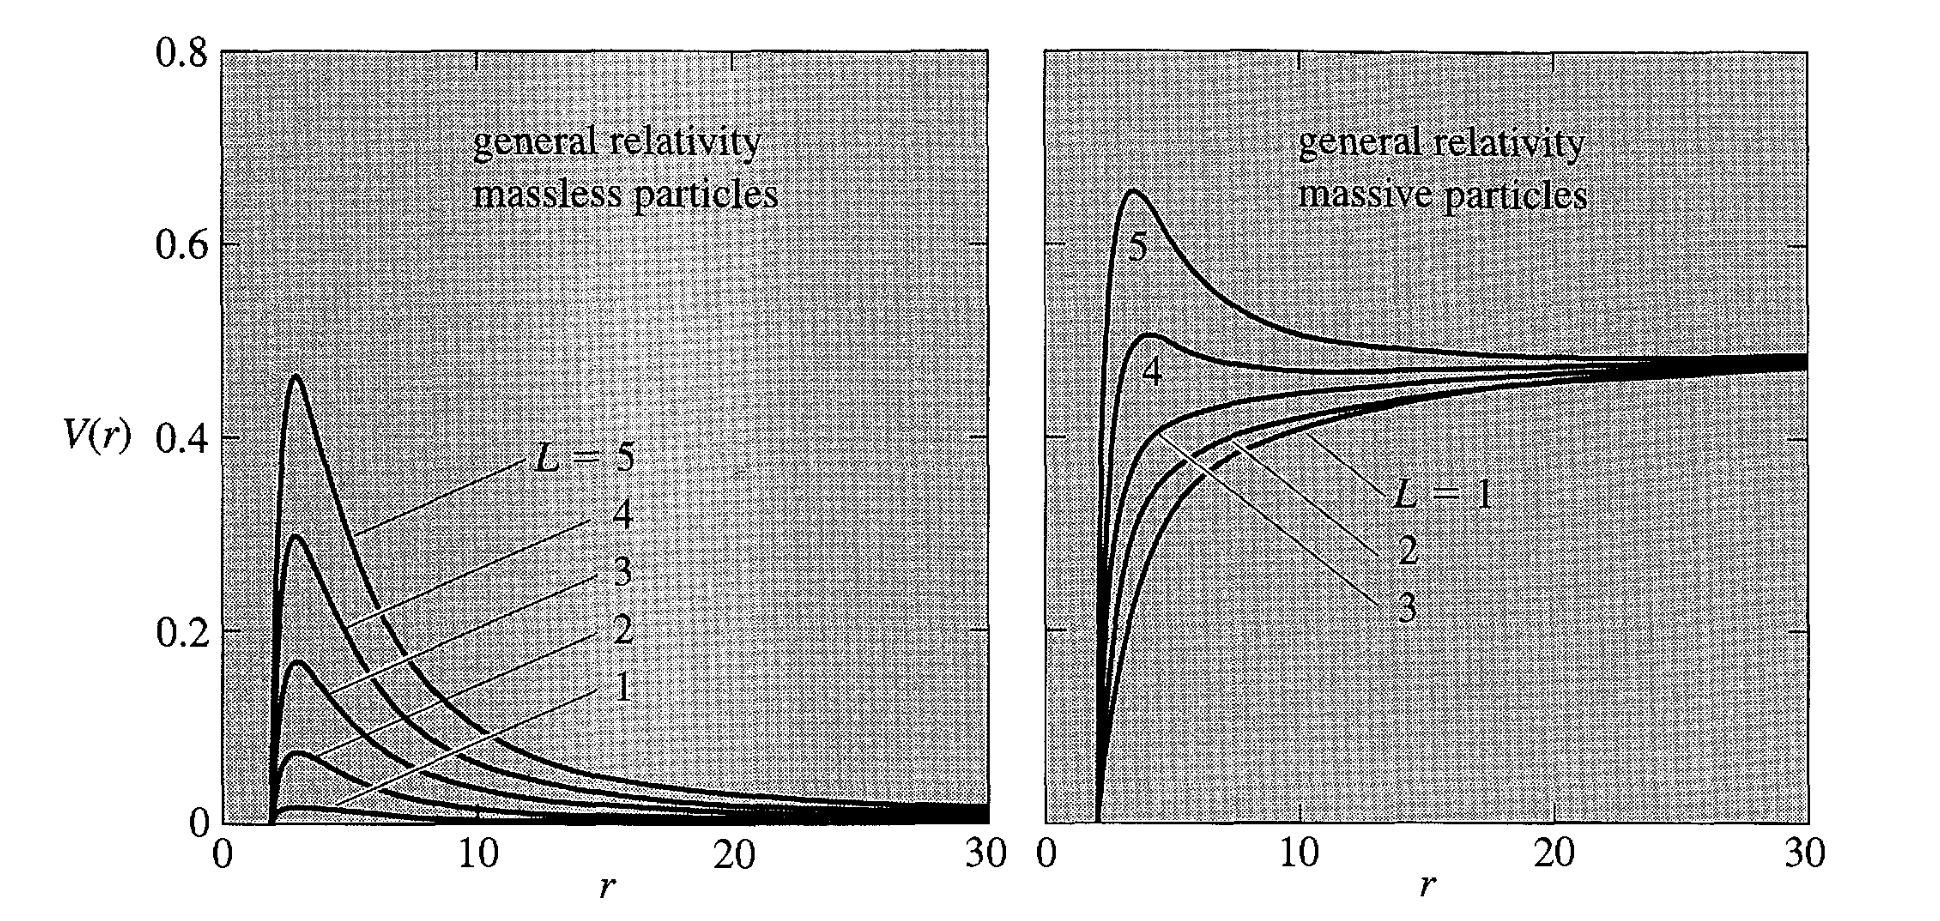
\includegraphics[scale=0.2]{GR/EP1.png}
\caption{Effective potentials in general relativity. We have chosen $M = 1$. In GR there is an innermost circular orbit greater than or equal to $3M$, and any orbit that falls inside this radius continues to $r = 0$ (for particles on geodesies).}
\end{figure}

\noindent
In general relativity, at $r = 2M$ the potential is always zero; inside this radius is the black hole.
For massless particles there is always a barrier (except for $L = 0$, for which the potential vanishes identically), but a sufficiently energetic photon will  nevertheless go over the barrier and be dragged inexorably down to the center. At the top of the barrier are unstable circular orbits $r_{\rm c} = 3M$.
\\ \\
For massive particles, the circular orbits are at
\[r_{\rm c} = \frac{L^2 \pm \sqrt{L^4-12M^2L^2}}{2M}.\]
For large $L$ there will be two circular orbits, one stable and one unstable. In the $L \to \infty$ limit their radii are given by $r_{\rm c} = \left(L^2/M, 3M \right)$.
In this limit the stable circular orbit becomes farther away, while the unstable one approaches $3M$, behaviour that parallels the massless case. As we decrease $L$,
the two circular orbits come closer together; they coincide when $L = \sqrt{12}M$ for which $r_{\rm c} = 6M$. We have therefore found that the Schwarzschild solution possesses stable circular orbits for $r > 6M$ and unstable circular orbits for $3M < r < 6M$. 
It's important to remember that these are only the geodesies; there is nothing to stop an accelerating particle from dipping below $r = 3M$ and emerging, as long as it stays beyond $r = 2M$.
\\ \\
As for a general non-circular orbit, we have the equation for orbit
\[\left(\frac{dr}{d\phi}\right)^2 + \frac{1}{L^2}r^4 - \frac{2M}{L^2}r^3 + r^2 - 2Mr = \frac{2E}{L^2}r^4. \] 
Define $x \equiv L^2/Mr$, we can get
\[\left(\frac{dx}{d\phi}\right)^2 + \frac{L^2}{M^2} - 2x + x^2 - \frac{2M^2}{L^2}x^3 = \frac{2EL^2}{M^2}. \]
Then we differentiate equation above with respect to $\phi$ to get
\[\frac{d^2x}{d\phi^2} - 1 + x = \frac{3M^2}{L^2}x^2.\]
In a Newtonian calculation, the last term would be absent, and we could solve for $x$ exactly; here, we suppose the orbit is far from horizon and treat it as a perturbation.
We expand $x$ into a Newtonian solution plus a small deviation, $x = x_0 + x_1$. The solution for the zeroth-order equation can be written as
\[x_0 = 1 + e\cos\phi.\]
Thus the first-order equation will be
\[\frac{d^2x_1}{d\phi^2} + x_1 = \frac{3M^2}{L^2}(1+e\cos\phi)^2.\]
After some approximation, we can get
\[x = 1 + e\cos((1-\alpha)\phi),\]
where $\alpha = 3M^2/L^2$. During each orbit, perihelion 
advances by an angle
\[\Delta \phi = 2\pi \alpha = \frac{6\pi M^2}{L^2}.\]
An ordinary ellipse satisfies
\[r = \frac{(1-e^2)a}{1+e\cos\phi},\]
where $a$ is the semi-major axis. Comparing to our zeroth-order solution and the definition of $x$, we see that
\[L^2 \approx M(1-e^2)a.\]
Finally, we have
\[\Delta \phi = \frac{6\pi M}{(1-e^2)a}.\]

\begin{figure}[!htb]
\centering
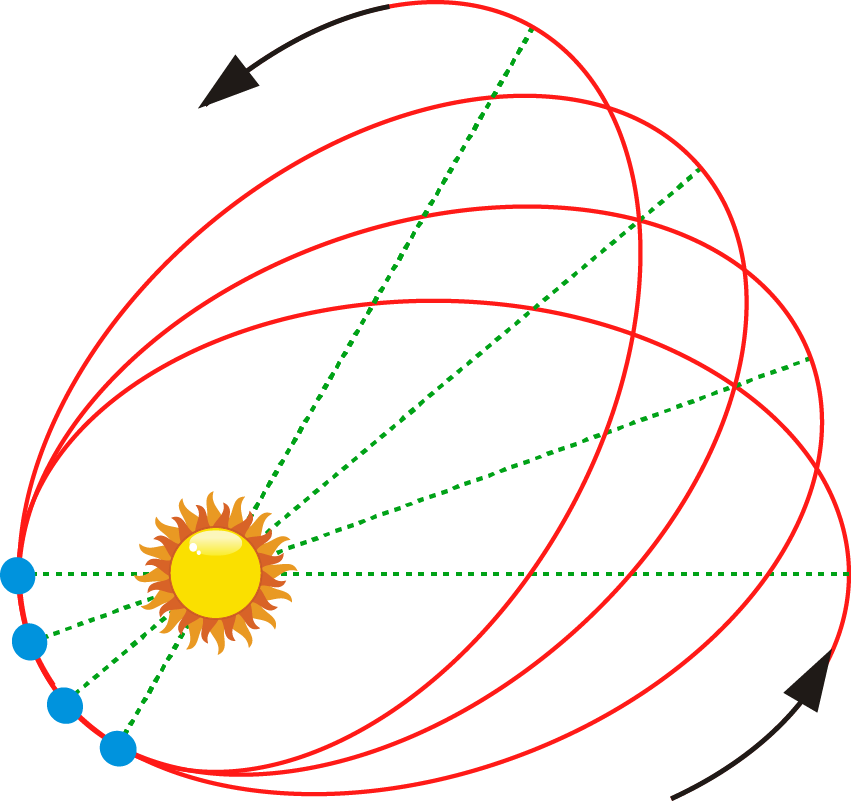
\includegraphics[scale=0.35]{GR/perihelion.png}
\caption{Perihelion of Mercury.}
\end{figure}

\subsection{Penrose diagram and event horizon}
In theoretical physics, a Penrose diagram is a two-dimensional diagram capturing the causal relations between different points in spacetime. 
It is an extension of a Minkowski diagram where the vertical dimension represents time, and the horizontal dimension represents space, and slanted lines at an angle of $45^{\circ}$ correspond to light rays. 
The biggest difference is that locally, the metric on a Penrose diagram is conformally equivalent to the actual metric in spacetime. 
The conformal factor is chosen such that the entire infinite spacetime is transformed into a Penrose diagram of finite size. 
For spherically symmetric spacetime, every point in the diagram corresponds to a $2$-sphere.
\\ \\
The metric of Minkowski space-time is 
\[ds^2 = -dt^2 + dr^2 + r^2 d\Omega^2.\]
Introduce the new coordinates $T$ and $R$ by 
\[t + r = \tan \frac{T+R}{2} ,\quad t - r = \tan \frac{T-R}{2}.\]
The metric can be written as
\[ds^2 = \frac{-dT^2+dR^2}{4\cos^2\frac{T+R}{2} \cos^2 \frac{T-R}{2}} + r^2(T,R) d\Omega^2.\]
The range of the new coordinates are $0 \leq R < \pi$ and  $|T| + R < \pi$.

\begin{figure}[!htb]
\centering
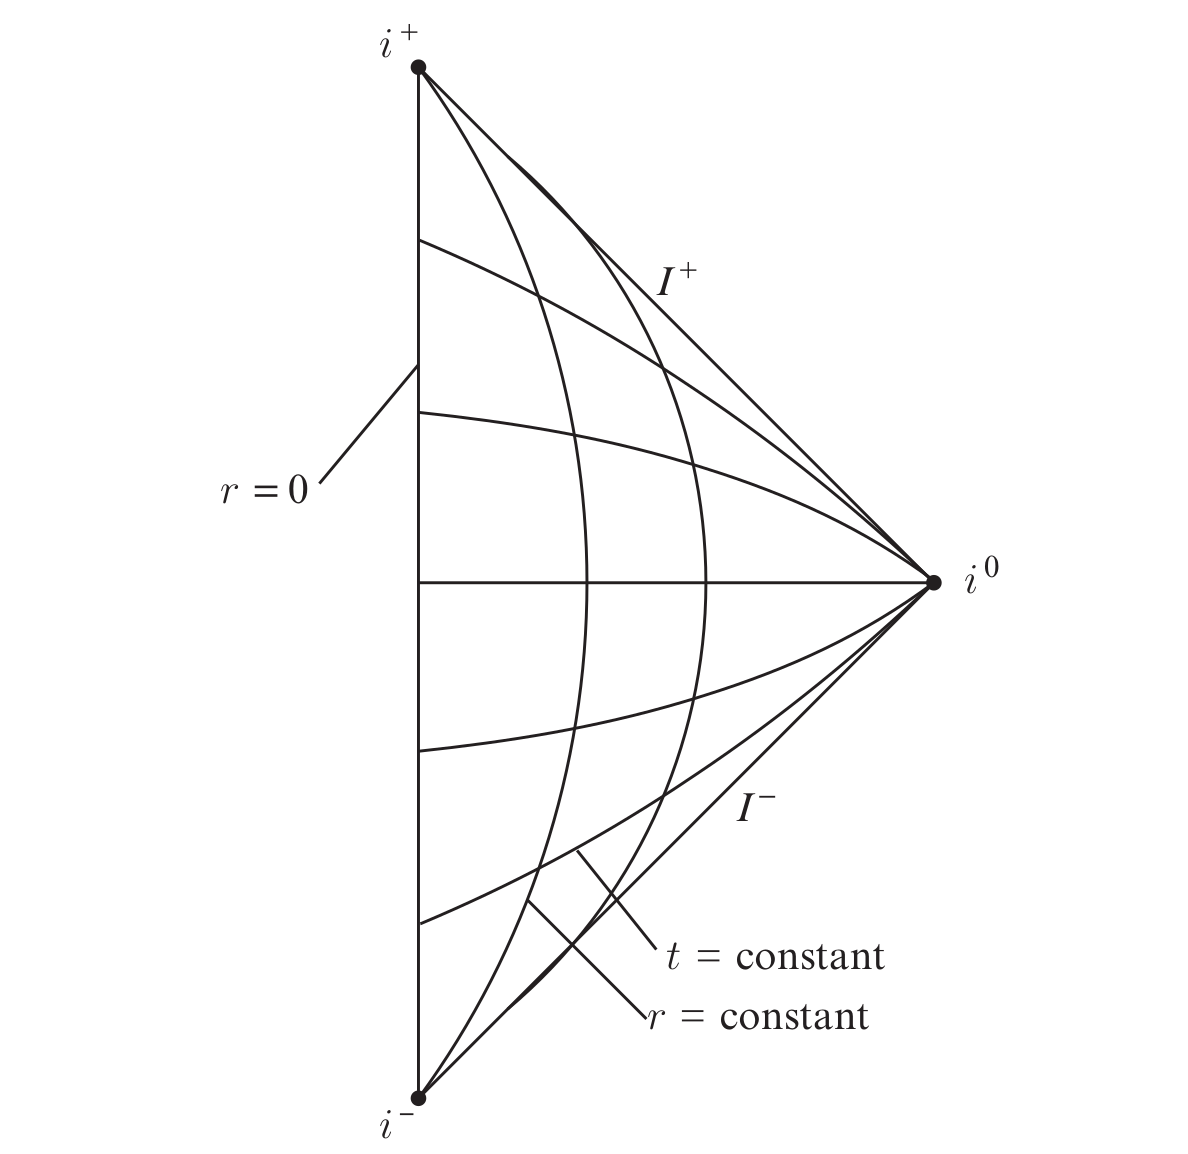
\includegraphics[scale=0.15]{GR/Penrose1.png}
\caption{Penrose diagram of Minkowski spacetime}
\end{figure}

\noindent
It is obvious that light cones are still 45 degree lines in this Penrose diagram. 
What is more, points and regions located at infinite distances in the original coordinates have now been brought to a finite distance. 
The figure indicates a set of different kinds of ``infinity'' that is useful in the discussion of physical phenomena. The following list gives the definition of each of these.
\begin{eqnarray}
i^{+} &=& \mbox{ future timelike infinity } (T = \pi, R = 0) \nonumber \\
i^{0} &=& \mbox{ spatial infinity } (T = 0, R = \pi) \nonumber \\
i^{-} &=& \mbox{ past timelike infinity } (T = -\pi, R = 0) \nonumber \\
I^{+} &=& \mbox{ future null infinity } (T = \pi - R, 0 < R < \pi) \nonumber \\
I^{-} &=& \mbox{ past null infinity } (T = -\pi + R, 0 < R < \pi) \nonumber
\end{eqnarray}
\\
Black holes are characterized by the fact that you can enter them, but never exit. 
Thus, their most important feature is actually not the singularity at the center, but the event horizon at the boundary. 
An event horizon is a hypersurface separating those spacetime points that are connected to infinity by a timelike path from those that are not. 
In general relativity, the global structure of spacetime can take many different forms, with correspondingly  different notions of infinity. 
But to think about black holes in the real universe, we use infinity as a proxy for ``well outside the black hole,'' and imagine that spacetime sufficiently far away from the hole can be approximated by Minkowski space.
\begin{figure}[!htb]
\centering
\includegraphics[scale=0.25]{GR/Penrose2.eps}
\caption{Penrose diagram of event horizon}
\end{figure}

\noindent
From Penrose diagram, the future event horizon is the surface beyond which timelike curves cannot escape to infinity. 
The causal past $J^{-}$ of a region is the set of all points we can reach from that region by moving along past-directed timelike paths, the event horizon can be
equivalently defined as the boundary of $J^{-}(I^+)$, the causal past of future null infinity. Analogous definitions hold for the past horizon. From the definition, it is clear that the event horizon is a null hypersurface.

\subsection{The maximally extended Schwarzschild solution}
Let us consider radial null curves, those for which $\theta$ and $\phi$ are constant and $ds^2 = 0$. We can get
\[\frac{dt}{dr} = \pm \left(1 -\frac{2M}{r} \right)^{-1}\]
For large $r$ the slope is $\pm$, as it would be in flat space, while as we approach $r = 2M$ we get $dt / dr = \pm \infty$, and the light cones ``close up''. 
Thus a light ray that approaches $r = 2M$ never seems to
get there, at least in this coordinate system; instead it seems to asymptote to this radius.

\begin{figure}[!htb]
\centering
\includegraphics[scale=0.3]{GR/BH1.eps}
\caption{In Schwarzschild coordinates, light cones appear to close up as we approach $r = 2M$.}
\end{figure}

\noindent
If we stayed outside while an intrepid observational general relativist dove into the black hole, sending back
signals all the time, we would simply see the signals reach us more and more slowly.

\begin{figure}[!htb]
\centering
\includegraphics[scale=0.3]{GR/BH2.eps}
\caption{A beacon falling freely into a black hole emits signals at intervals of constant proper time. An observer at fixed $r$ receives the signals at successively longer
time intervals.}
\end{figure}

\noindent
The fact that we never see the infalling observer reach $r = 2M$ is a meaningful statement, but the fact that their trajectory in the $t-r$ plane never reaches there is not. 
It is highly dependent on our coordinate system, and we would like to ask a more coordinate-independent question (such as, ``Does the observer reach this radius in a finite amount of their proper time?''). 
The best way to do this is to change coordinates to a system that is better behaved at $r = 2M$. We omit the intermediate steps of coordinate transformation and move to Kruskal coordinates directly. The new coordinates is given by
\[T = \left( \frac{r}{2M} -1 \right)^{1/2} e^{r/4M}\sinh \left( \frac{t}{4M}\right), \quad R = \left( \frac{r}{2M} -1 \right)^{1/2} e^{r/4M}\cosh\left( \frac{t}{4M}\right).\]
The metric becomes
\[ds^2 = \frac{32M^3}{r}e^{-r/2M}(-dT^2+dR^2) + r^2 d\Omega^2.\]
We can now draw a spacetime diagram in the $T-R$ plane, known as a Kruskal diagram. This diagram represents the maximal extension of the Schwarzschild geometry; the coordinates cover what we should think of as
the entire manifold described by this solution.

\begin{figure}[!htb]
\centering
\includegraphics[scale=0.3]{GR/BH3.eps}
\caption{The Kruskal diagram -- the Schwarzschild solution in Kruskal coordinates, where all light cones are at $\pm 45^{\circ}$.}
\end{figure}

\noindent
\\
Finally, we can further transform the coordinates to bring them into a finite range and get the Penrose diagram of Schwarzschild spacetime.

\begin{figure}[!htb]
\centering
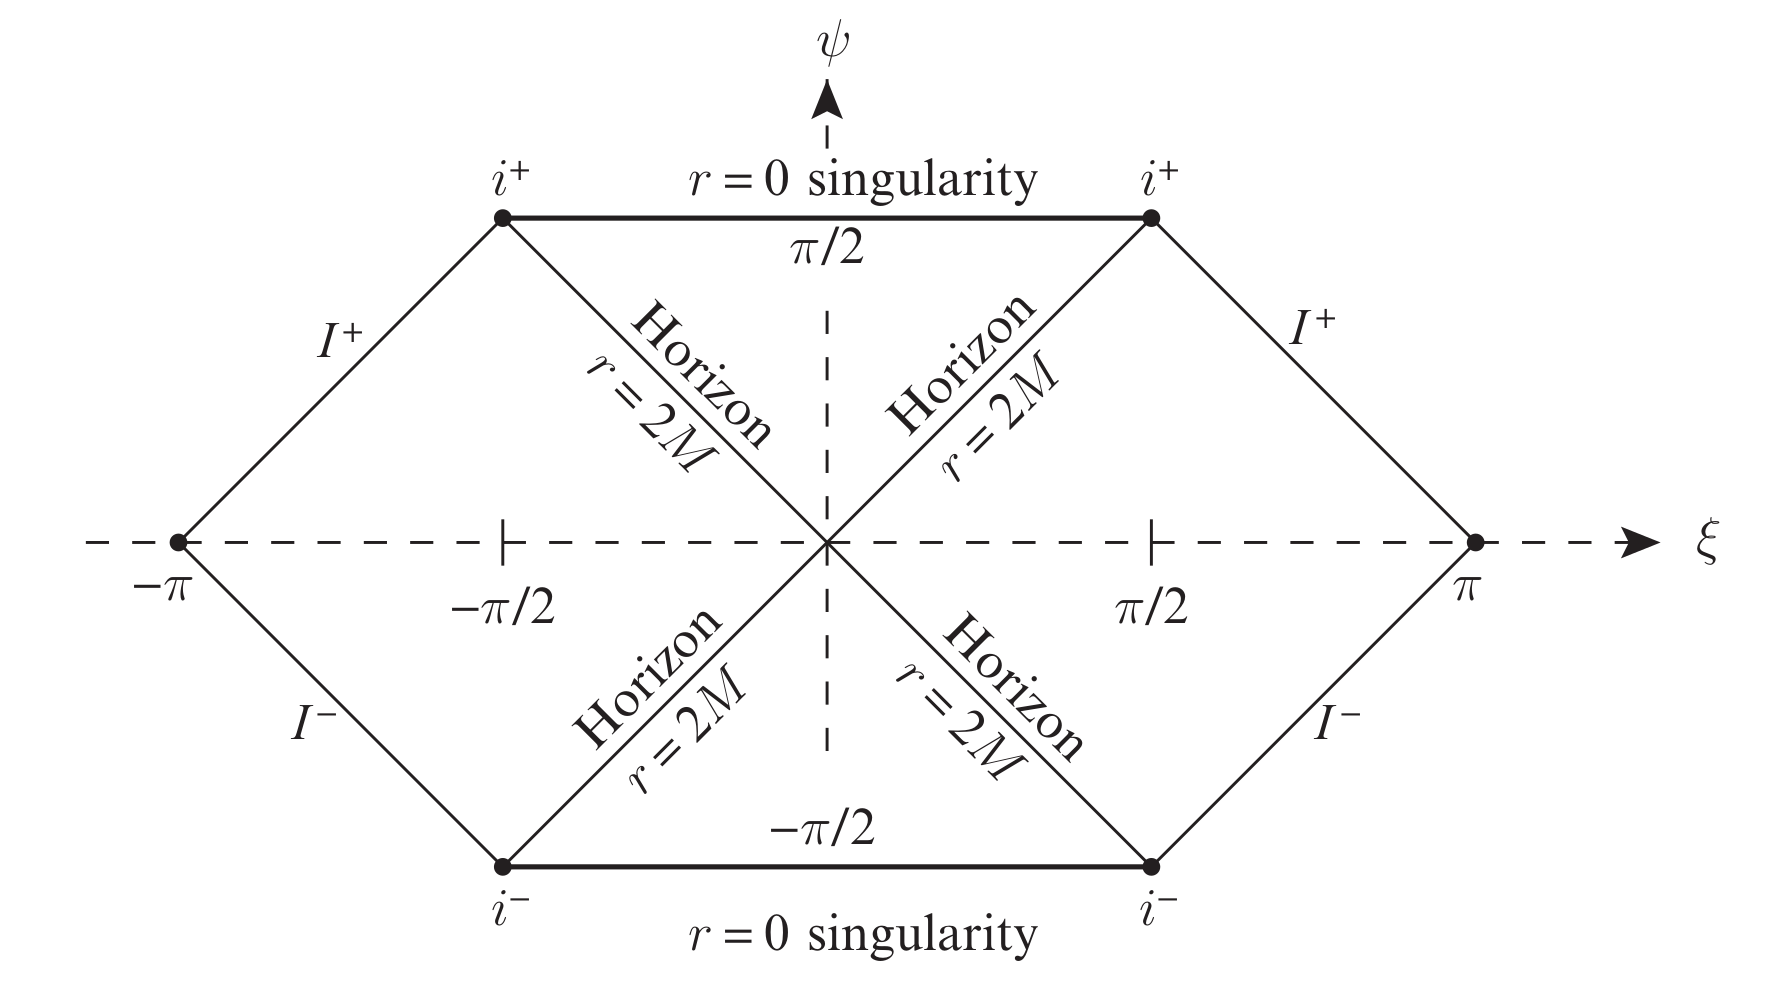
\includegraphics[scale=0.15]{GR/BH4.png}
\caption{The Penrose diagram for the Schwarzschild spacetime.}
\end{figure}

\section{Reissner-Nordstrom black hole}
The metric of Reissner-Nordstrom black hole is
\[ds^2 = -\Delta dt^2 + \Delta^{-1}dr^2 + r^2d\Omega^2,\]
where
\[\Delta = 1 - \frac{2M}{r} + \frac{Q^2}{4 \pi r^2}.\]
The EM filed is given by
\[A_{t} = -\frac{Q}{4\pi r}.\]
The RN metric has a true curvature singularity at $r = 0$, as could be checked by computing the curvature invariant scalar $R^{\mu\nu\rho\sigma}R_{\mu\nu\rho\sigma}$. 
The horizon of RN metric is given by $g^{rr} = 0$, i.e.
\[1 - \frac{2M}{r} + \frac{Q^2}{4 \pi r^2} = 0.\]
\\
If $M^2 > Q^2 / 4 \pi$, the metric coefficient $\Delta$ is positive at large $r$ and small $r$, and negative inside the two vanishing points $r_{\pm} = M \pm \sqrt{M^2 - Q^2 / 4 \pi}$. 
The metric has coordinate singularities at both $r_{+}$ and $r_{-}$; in both cases these could be removed by a change of coordinates as we did with Schwarzschild.
The surfaces defined by $r_{\pm}$ are both null, and they are both event horizons. 
The singularity at $r = 0$ is a timelike line, not a spacelike surface as in Schwarzschild. 
If you are an observer falling into the black hole from far away, $r_{+}$ is just like $2M$ in the Schwarzschild metric; at this radius $r$ switches from being a spacelike coordinate to a timelike coordinate, and you necessarily move in the direction of decreasing $r$. 
Witnesses outside the black hole also see the same phenomena that they would outside an uncharged hole --- the infalling observer is seen to move more and more slowly, and is increasingly redshifted.
\\ \\
But the inevitable fall from $r_{+}$ to ever-decreasing radii only lasts until you reach the null surface $r = r_{-}$, where $r$ switches back to being a spacelike 
coordinate and the motion in the direction of decreasing $r$ can be arrested. 
You can choose either to continue on to $г = 0$, or begin to move in the direction of increasing $r$ back through the null surface at $r = r_{-}$.
Then $r$ will once again be a timelike coordinate, but with reversed orientation; you are forced to move in the
direction of increasing $r$. 
You will eventually be spit out past $r = r_{+}$ once more, which is like emerging from a white hole into the rest of the universe.
From here you can choose to go back into the black hole --- this time, a different hole than the one you entered in the first place --- and repeat the voyage as many times as you like.
\\ \\
If $M^2 = Q^2 / 4 \pi$, the extremal black holes have $\Delta = 0$ at a single radius, $r = M$. 
This represents an event horizon, but the $r$ coordinate is never timelike; it becomes null at $r = M$, but is spacelike on either side. 
The singularity at $r = 0$ is a timelike line, as in the other cases.
 Thus for this black hole you can again avoid the singularity and continue to move to the future to extra copies of the asymptotically flat region, but the singularity is always ``to the left''. 
\\ \\
If $M^2 < Q^2 / 4 \pi$, $\Delta$ is always positive and the metric is completely all the way down to $r = 0$. 
The coordinate $t$ is always timelike, and $r$ is always spacelike. But still there is the singularity at $r = 0$, which is now a timelike line. 
Since there is no event horizon, there is no obstruction to an observer traveling to the singularity and returning to report on what was observed. 
This is a naked singularity. 
A careful analysis of the geodesies reveals that the singularity is repulsive--timelike geodesies never intersect $r = 0$; instead they approach and then reverse course and move away. 
Null geodesies can reach the singularity, as can nongeodesic timelike curves.
As $r \to \infty$ the solution approaches flat spacetime, and as we have just seen the causal structure seems normal everywhere. 
The conformal diagram will therefore be just like that of Minkowski space, except that now $r = 0$ is a singularity.

\begin{figure}[!htb]
\centering
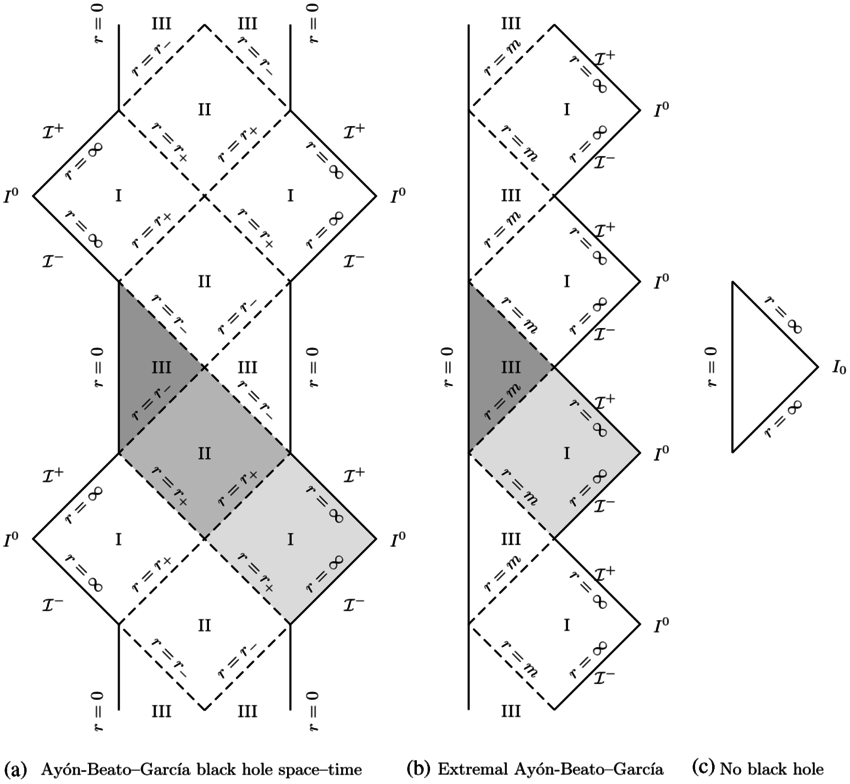
\includegraphics[scale=0.4]{GR/BH5.png}
\caption{Penrose diagram of RN spacetime}
\end{figure}

\section{Kerr black hole}
\subsection{Geometry of Kerr black hole}
The metric of Kerr black hole is
\begin{eqnarray}
    ds^2 &=& -\left(1 - \frac{2Mr}{\rho^2}\right)dt^2 - \frac{2Mar\sin^2\theta}{\rho^2}(dt d\phi + d\phi dt) + \frac{\rho^2}{\Delta} dr^2
    \nonumber \\
    &+& \rho^2d\theta^2 + \frac{\sin^2\theta}{\rho^2} \left[(r^2+a^2)^2 - a^2 \Delta \sin^2\theta\right]d\phi^2,
    \nonumber 
\end{eqnarray}
where
\[\Delta(r) = r^2 - 2Mr + a^2, \quad \rho^2(r,\theta) = r^2 + a^2 \cos^2\theta.\]
We can show that $a$ is the the angular momentum per unit mass of the black hole.
\\ \\
It is straightforward to check that as $a \to 0$ they reduce to Schwarzschild coordinates.
If we keep $a$ fixed and let $M \to 0$, we recover flat spacetime but not in ordinary polar coordinates. 
The metric becomes
\[ds^2 = -dt^2 + \frac{r^2+a^2\cos^2\theta}{r^2 + a^2} dr^2 + (r^2 + a^2\cos^2\theta)^2d\theta^2 + (r^2+a^2)\sin^2\theta d\phi^2,\]
and we recognize the spatial part of this as flat space in ellipsoidal coordinates. 
They are related to Cartesian coordinates in Euclidean $3$-space by
\begin{eqnarray}
x &=& (r^2+a^2)^{\frac{1}{2}} \sin\theta \cos\phi \nonumber \\
y &=& (r^2+a^2)^{\frac{1}{2}} \sin\theta \sin\phi \nonumber \\
z &=& r\cos\theta. \nonumber
\end{eqnarray}
$r = 0$ is a two-dimensional disk; the intersection of $r = 0$ with $\theta = \pi / 2$ is the ring at the boundary of this disk.
\\ \\
There are two Killing vectors of the metric, $K = \partial_t$ and $R = \partial_{\phi}$. The norms of these Killing vectors are scalar quantities with a coordinate-free, geometrical interpretation. 
This allows us to represent three of the metric coefficients in the form
\begin{eqnarray}
K^2 &=& g_{tt} = -\left( \frac{\Delta - a^2\cos^2\theta}{\rho^2} \right), \nonumber \\
K\cdot R &=& g_{t\phi} = \frac{a\sin^2\theta(\Delta - a^2 - r^2)}{\rho^2}, \nonumber \\
R^2 &=& g_{\phi\phi} = \frac{[(r^2+a^2)^2-\Delta a^2\sin^2\theta]\sin^2\theta}{\rho^2}. \nonumber
\end{eqnarray}
From the form of the Kerr metric, it is obvious that the metric becomes ill-defined at $\rho = 0$ and at $\Delta = 0$.
The calculation of scalar invariants of the curvature tensor shows that $\rho = 0$ is indeed a physical singularity. The condition $\rho = 0$ corresponds to
\[\rho^2 = r^2 + a^2\cos^2\theta = 0,\]
which can only be satisfied with $\theta = \pi/2$ and $r = 0$. Hence we have a ring-like singularity in the case of a Kerr metric. 
The curvature invariants are well behaved at $\Delta = 0$. 
$\Delta(r) = 0$ is equal to $g^{rr} = 0$. 
Thus $\Delta(r) = 0$ is a null surface.
The quadratic equation $\Delta = 0$ has two roots if $|a| < M$,
\[r_{\rm hor} = M \pm \sqrt{M^2-a^2},\]
representing inner and outer horizons in Kerr spacetime.
\\ \\
Let us consider the surface defined by the quadratic equation $g_{tt} = 0$. 
Consider a class of observers with four-velocity $u$ in the direction of the timelike Killing vector $K$. 
For any photon with four-momentum $p$ propagating in this spacetime, the observer with four-velocity $u$ will attribute a frequency
\[\omega = -p^{\mu}u_{\mu} =  \frac{p^{\mu}K_{\mu}}{K^{\mu}K_{\mu}} = \frac{E}{-g_{tt}}\]
where $E$ is the conserved ``energy'' of the photon. Thus it is easy to see that the surface with $g_{tt} = 0$ corresponds to infinite redshift.
For the Kerr metric, the equation $g_{tt}$ also has two solutions, $r = r_{\pm}$, given by
\[r_{\pm} = M \pm \sqrt{M^2-a^2\cos^2\theta}.\]
Physically, this corresponds to a surface of infinite redshift usually called an ergosurface.
The region between outer ergosurface and horizon is called the ergosphere.

\begin{figure}[!htb]
\centering
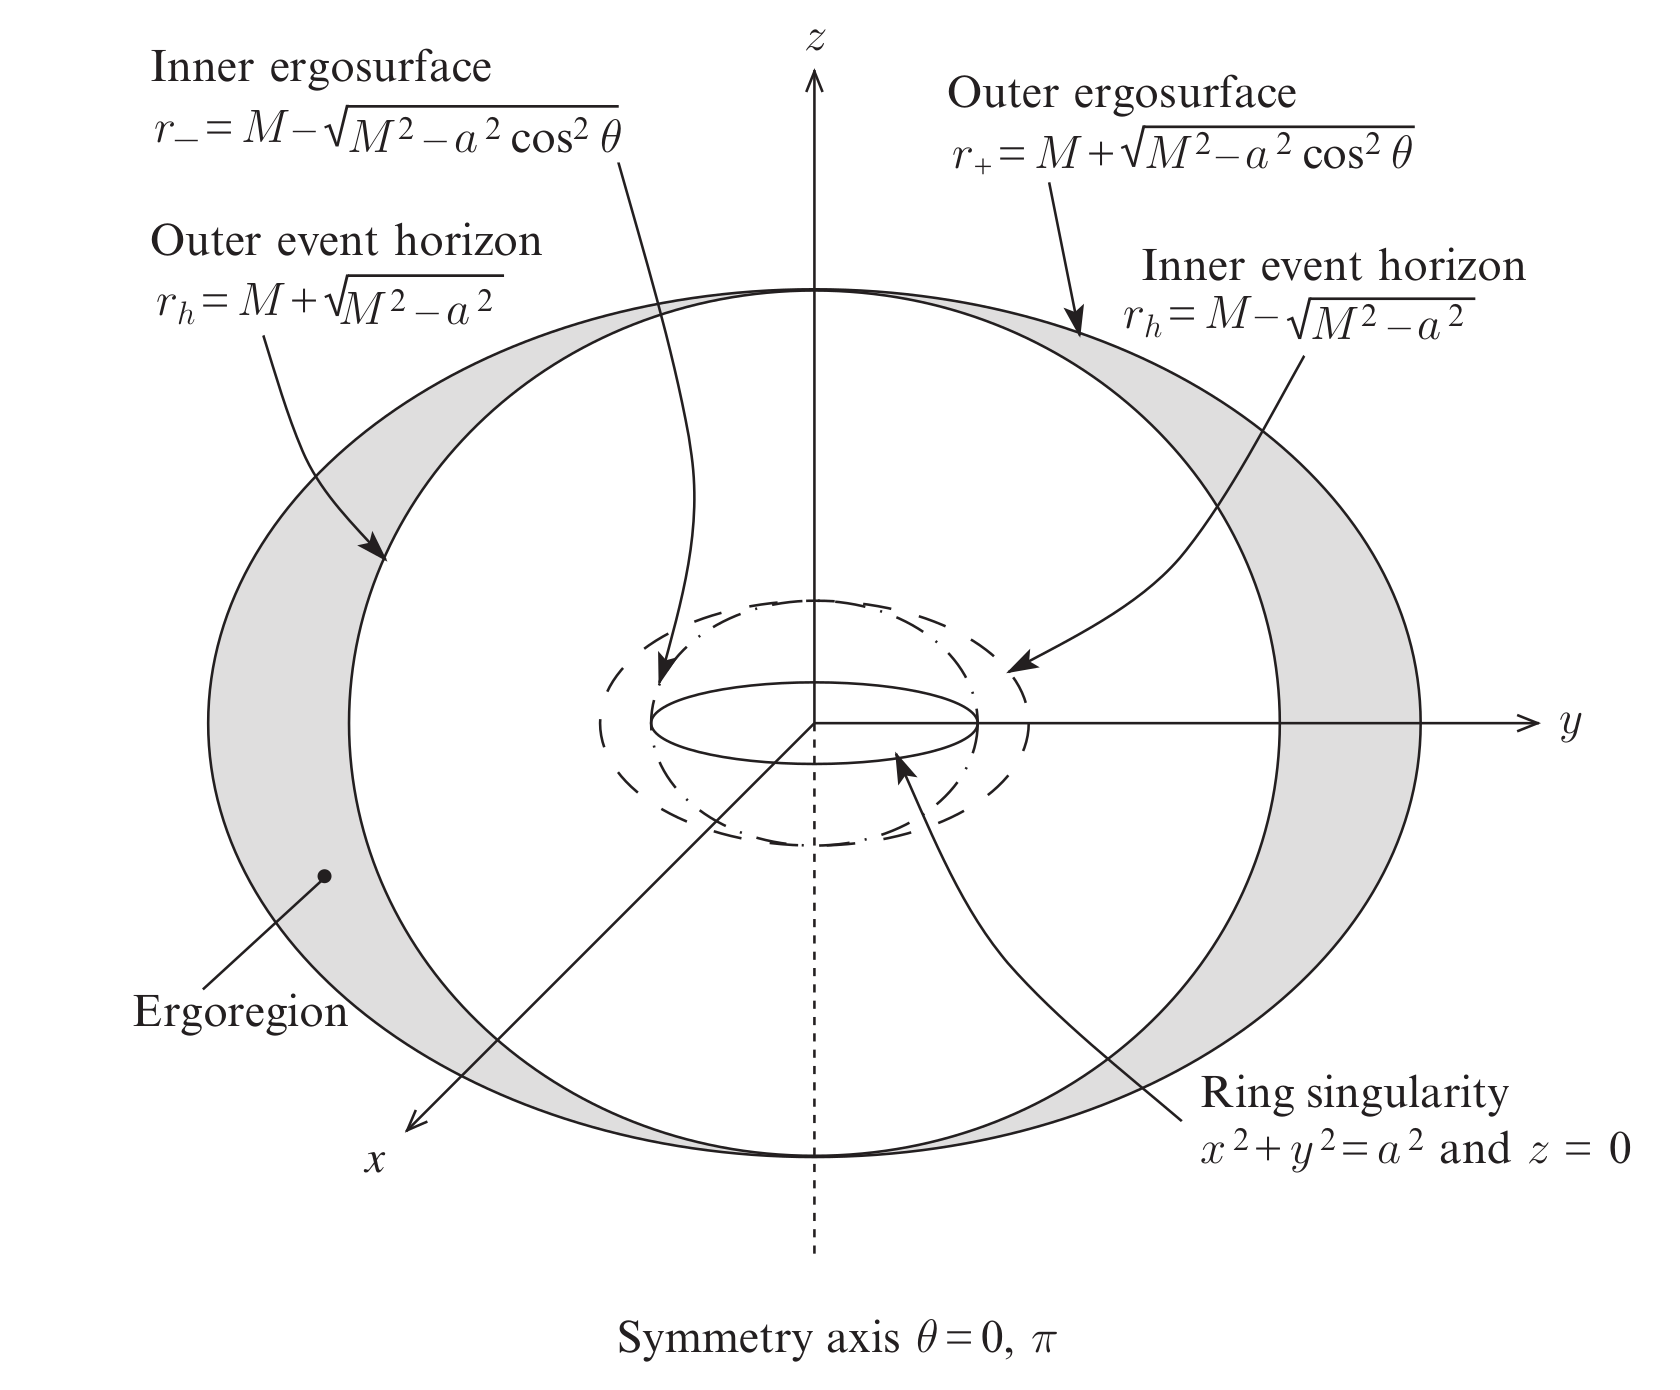
\includegraphics[scale=0.15]{GR/BH6.png}
\caption{Schematic picture showing the geometrical structure of the Kerr spacetime.}
\end{figure}

\begin{figure}[!htb]
\centering
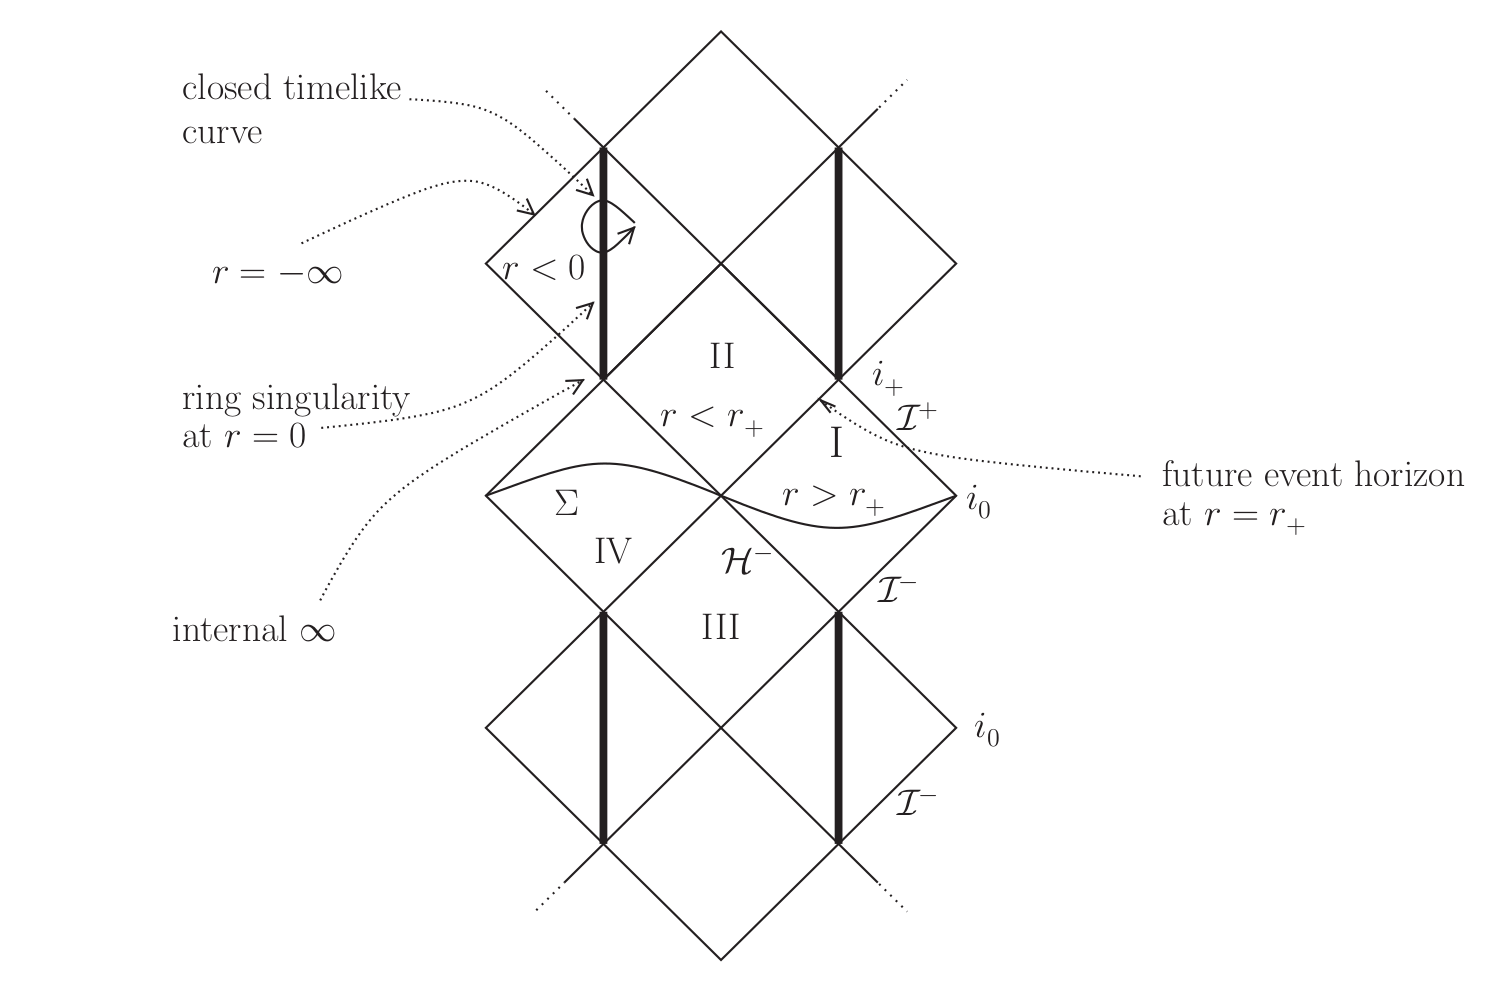
\includegraphics[scale=0.2]{GR/BH7.png}
\caption{The Penrose-Carter diagram for the Kerr spacetime for the case $M > a$.}
\end{figure}

\subsection{Static limit}
An observer in the Kerr spacetime moving with a constant angular velocity and having fixed values for $r$, $\theta$ will see the geometry to be unchanging. 
Such observers are called stationary observers. 
If the observers also have a fixed value for $\phi$, they are called static observers located at fixed spatial coordinates.
\\ \\
Consider a stationary observer with an angular velocity $\Omega$ in the Kerr spacetime with
\[\Omega = \frac{d\phi}{dt} = \frac{u^{\phi}}{u^{t}}.\]
Such an observer has a four-velocity $(u^{t},0,0,\Omega u^{t})$. From the normalization $u^{\mu}u_{\mu} = -1$, we have
\[g_{tt} + 2g_{t\phi}\Omega + g_{\phi\phi} \Omega^2 < 0.\]
This condition leads to limits in the range of values allowed for the angular velocity to be
\[\Omega_{\rm min} < \Omega < \Omega_{\rm max},\]
where
\[\Omega_{\rm min} = \omega - \sqrt{\omega^2 - (g_{tt}/g_{\phi\phi})}, \quad \Omega_{\rm max} = \omega + \sqrt{\omega^2 - (g_{tt}/g_{\phi\phi})},\]
with
\[\omega = -\frac{g_{\phi t}}{g_{\phi\phi}} = \frac{2Mar}{(r^2+a^2)^2-\Delta a^2\sin^2\theta}.\]
First, far away from the black hole, we have $r\Omega_{\rm min} = -1$ and $r\Omega_{\rm max} = +1$, which correspond to the standard result that motion should be at a speed less than that of light. 
Second, as one moves closer to the black hole, $\Omega_{\rm min}$ increases due to the dragging of the
inertial frames. 
Eventually, $\Omega_{\rm min}$ reaches zero at the surface on which $g_{tt} = 0$, which is the ergosurface. 
Therefore, inside the ergosphere, all stationary observers
must orbit the black hole with $\Omega > 0$ and hence static observers can exist only out-side the ergosurface. 
Finally, as one crosses the ergosurface and moves towards the event horizon, the allowed range of angular velocities become ever more positive with the allowed range narrowing down. 
At the event horizon, the $\Omega_{\rm min}$ and $\Omega_{\rm max}$ coincide and all timelike worldlines point inwards. 
The limiting angular velocity is given by
\[\Omega_{\rm H} \equiv \omega_{r_{\rm h},\theta} = \frac{a}{2Mr_{\rm h}}.\]
This limiting angular velocity is sometimes called the angular velocity of the horizon. Using this we can form a new Killing vector
\[K' \equiv K + \Omega_{\rm H} R.\]
It is clear that this Killing vector becomes null on the event horizon and is timelike outside the horizon.

\subsection{Penrose process and the area of the event horizon}
Since the Kerr metric has a timelike Killing vector field $K$ any particle moving on a geodesic will have a conserved energy given by $E = -P_{\mu} K^{\mu} = -p_{t}$.
We can derive that the orbit must be inside the ergosphere if the energy has to be negative.
\\ \\
This result can be used to extract energy from the Kerr black hole in several ways, of which the simplest one is the following. 
Consider, for example, a particle A moving in the ergosphere which breaks into two particles B and C. 
We let particle B to fall into the black hole and let particle C escape to infinity. 
All this can be done using suitable timelike trajectories. The conservation of four-momentum requires that
\[E_{\rm A} = E_{\rm B} + E_{\rm C}.\]
Since the particle A can fall into the ergosphere from infinity, we have $E_{\rm A} > m$.
We can arrange the trajectory of B making $E_{\rm B} < 0$. It immediately follows that $E_{\rm C} > E_{\rm A}$. 
When the particle C goes back to infinity, it will have more energy than the original particle had. 
Thus, using the existence of negative energy orbits in the ergosphere and the local conservation of energy for processes taking place in the ergo region, one can extract energy from the black hole.
\\ \\
The Penrose process decreases both the mass and the angular momentum of the Kerr black hole by an amount equal to the (negative of) the energy and the angular momentum of the particle B that falls into the black hole. 
Consider the dot product of $p^{\mu}$ with the Killing vector $K'$. 
Since $K'$ is timelike outside the horizon and we want particle B to fall into the horizon, it is necessary that this dot product is negative. 
Using $p^{\mu}K_{\mu} = -E$, $p^{\mu}R_{\mu} = L$,
where $E$ and $L$ are the conserved energy and angular momentum of particle B, we get the condition $-E + \Omega_{\rm H} L < 0$. 
When the particle B falls into the black hole, the angular momentum and mass of a Kerr black hole will change by $\delta J = L$ and $\delta M = E$. Hence the above bound
translates into the result
\[\delta M > \Omega_{\rm H} \delta J.\]
\\
The surface area of the event horizon of a Kerr black hole is given by
\[A = 4\pi (r_{\rm h}^2 + a^2).\]
We can verify that
\[\delta A = 8\pi \frac{a}{\Omega_{\rm H}\sqrt{M^2-a^2}}(\delta M - \Omega_{\rm H} \delta J).\]
This can be manipulated to read
\[\delta M = \frac{\delta \kappa}{8\pi G} \delta A + \Omega_{\rm H}\delta J,\]
where
\[\kappa = \frac{\sqrt{M^2-a^2}}{2M(M+\sqrt{M^2-a^2})}\]
is the surface gravity. 
Quantum field theory in curved space time would show that this relation can be given a thermodynamic interpretation with $\kappa / 2\pi$ acting as the temperature of the black hole and $A/4$ acting as the entropy of the black hole.

\subsection{Particle orbits in the Kerr metric}
The orbits of particles in the Kerr metric can be studied, in principle, by the same techniques we have used in the case of the Schwarzschild metric. 
However, lack of spherical symmetry makes the nature of the orbits very complicated and analytic solutions are impossible to find. 
It is clear that radial motion will now be possible only along the axis of symmetry and even planar motion will be possible only in the equatorial plane. 
Derivations of equations that govern the particle trajectories in the Kerr metric is given by subsection $8.5.4$ of \emph{Gravitation: Foundations and Frontiers ( T. Padmanabhan)}.
\\ \\
The existence of stable circular orbits in the equatorial plane is of some practical interest in astrophysics. 
It is generally believed that the matter in the accretion
disks around astrophysical black holes will be able to move towards the black hole in a series of approximately circular orbits in the equatorial plane. 
In that case, the radius of the stable circular orbit closest to the black hole and its energy are
of interest in the astrophysics of accretion disks. 
For the motion in the equatorial plane one can introduce an effective potential as in the case of the Schwarzschild
metric along the following lines. Setting $\theta = \pi / 2$ into equations of motion will give equation for the radial motion,
\[m^2 \left(\frac{dr}{d\tau} \right)^2 = \frac{[(r^2+a^2)E-aL]^2}{r^4} - \frac{\Delta[(aE-L)^2+m^2 r^2]}{r^4}.\]
We can now define an effective $U(r)$ such that the right hand side of the above equation vanishes when $E=U$. 
Hence the effective potential is the solution to the
equation:
\[[(r^2+a^2)U(r)-aL]^2 - \Delta[(aU(r)-L)^2+m^2 r^2] = 0.\]
The radii of stable circular orbits are determined by the minima of $U(r)$; that is by the simultaneous solution to the equations $E = U(r)$, $U'(r) = 0$. 
Among all the stable circular orbits, we are interested in the innermost one. 
Fairly lengthy but straightforward calculation shows that this orbital radius is the solution to the quartic equation
\[r^2 - 6Mr - 3a^2 \mp 8a\sqrt{Mr} = 0,\]
where the upper (lower) sign corresponds to the counter-rotating (co-rotating) orbit.
When $a = 0$ we get the standard result that $r = 6M$; as the rotation parameter increases, the radius of the circular orbit decreases for the co-rotating orbit which is the one that is probably the relevant one for the accretion disk. 
This shows that one can have stable circular orbits very
close to the black hole in the case of rotating black holes. 
The quantity $(m-E)/m$ represents the fraction of the rest energy that can be released when a particle falls from the innermost stable circular orbit into the black hole. 
In the extreme case of $a = M$, this fraction is $1 - 1 / \sqrt{3}$ which is about $42$ percent, while the corresponding value for orbits in the Schwarzschild metric is only about $5.7$ percent. 
This higher efficiency could be of use in certain astrophysical scenarios.

\chapter{Geometry of the Universe}
\section{Friedmann–Lemaître–Robertson–Walker metric}
The metric in standard model of cosmology is
\[ds^2 = -dt^2 + a(t)^2 \left(\frac{dr^2}{1-Kr^2} + r^2 d\Omega^2 \right).\]
If we define
\[\chi \equiv \begin{cases} 
\sin^{-1}(\sqrt{K}r)/\sqrt{K}, K > 0 \\
r, K = 0 \\
\sinh^{-1}(\sqrt{-K}r)/\sqrt{-K}, K < 0
\end{cases}\]
and
\[\eta \equiv \int \frac{dt}{a(t)},\]
the metric can then be written as
\[ds^2 =  a(\eta)^2 \left(-d\eta^2 + d\chi^2 + r(\chi)^2 d\Omega^2 \right).\]
In coordinates $(t,r,\theta,\phi)$, we have
\[G_{tt} = \frac{3(\dot{a}^2+K)}{a^2}, \quad G^{\mu}_{\mu} = -\frac{6(\dot{a}^2+a\ddot{a}+K)}{a^2}.\]  
Suppose that the matter in the universe can be modelled as idealized fluid. Thus the corresponding energy-momentum tensor is $T^{\mu\nu} = (\rho + p) u^{\mu} u^{\nu} + pg^{\mu\nu}$. Contraction of the energy-momentum tensor gives $T^{\mu}_{\mu} = -\rho + 3p$. 
If the matter is comoving with the coordinates, we have $T_{tt} = \rho$. Einstein equations now takes the from as
\[\left(\frac{\dot{a}}{a} \right)^2 = \frac{8\pi}{3}\rho - \frac{K}{a^2}, \quad \frac{\ddot{a}}{a} = - \frac{4\pi}{3}(\rho + 3p),\]
called Friedmann equations. If we take the derivative of the first equation, we can get
\[\frac{\ddot{a}}{a} = -\frac{4\pi}{3}\left( - \frac{d\rho}{d \ln a} -2\rho \right).\]
By comparing with the second equation, we have
\[\frac{d\rho}{d \ln a} = -3(p+\rho).\]
If we have the equation of state $p = k\rho$, then it is easy to verify that $\rho \propto a^{-3(k+1)}$.
As for radiation (photon), we have $p_{\rm R} = 1/3 \rho_{\rm R}$, so $\rho_{\rm R} \propto a^{-4}$. As for cold matters (baryon, cold dark matter), we have $p_{\rm CM} = 0$, so $\rho_{\rm CM} \propto a^{-3}$. As for dark energy, we have $p_{\rm DE} = - \rho_{\rm DE}$, so $\rho_{\rm DE} = $ constant. Our universe is mainly composed of dark energy, cold dark matters, baryons and radiations. 
The Friedmann equations can be now written as
\[\frac{H^2}{H_0^2} = \Omega_{\rm R0}a^{-4} + \Omega_{\rm CM0} a^{-3} + \Omega_{\rm DE0} + \Omega_{\rm K0}a^{-2}.\]
In equation above, the subscript $0$ denotes today's value of some parameters and we scale the coordinates to make $a_0 = 1$. 
$H \equiv \dot{a} / a$ and $H_0$ is called Hubble's constant. $\Omega_0$ is the ratio between density $\rho_0$ of some substance and critical density $\rho_{\rm c0} \equiv {3H_0^2}/{8\pi}$. Particularly, $\rho_{\rm K0} = 3K/8\pi$ is called the density of curvature energy and we can note that $\Omega_{\rm K0} = 1 - \Omega_{\rm DE0} - \Omega_{\rm CM0} - \Omega_{\rm R0}$.

\section{Observable quantities}
\subsubsection{Redshift}
Suppose there is a photon emitted from $r=0$ at time $t$, then the world line of the photon will satisfy that
\[\left(\frac{dt}{dr}\right)^2 = \frac{a^2}{1-Kr^2}, \quad \theta = \mbox{ Constant}, \quad \phi = \mbox{ Constant}.\]
In terms of four-momentum, we have
\[\left(\frac{p^t}{p^r}\right)^2 = \frac{a^2}{1-Kr^2}\]
On the other hand, we have the geodesic equation that
\[\frac{dp^{t}}{d\lambda} + \Gamma^{t}_{\phantom{*}\alpha \beta} p^{\alpha}p^{\beta} = \frac{dp^{t}}{d\lambda} + \frac{a\dot{a}}{1-Kr^2}(p^r)^2 = 0.\]
It can be simplified to
\[\frac{dp^t}{p^t} + \frac{da}{a} = 0.\]
Note that $a_0 = 1$, so we have $p^t_0 = ap^t$. Define cosmological redshift by $p_0^t = p^t/(1+z)$. We have the relation
\[a = \frac{1}{1+z}.\]

\subsubsection{Luminosity}
Suppose there is an object with intrinsic luminosity $L$ at $r = 0$ and time $t$. Suppose at time $t_0$, the photon propagate to $r = r_0$(our position) at time $t_0$ (now). In coordinates $(\eta,\chi)$, we have $\eta_0 = \chi_0$. Thus
\[\chi_0(z) = \int_{t}^{t_0} \frac{dt'}{a} = \int_{0}^{z} \frac{dz'}{H(z')},\]
where $z$ is the redshift of the object and 
\[r_0 \equiv \begin{cases} 
\sin(\sqrt{K}\chi_0)/\sqrt{K}, K > 0 \\
\chi_0, K = 0 \\
\sinh(\sqrt{-K}\chi_0)/\sqrt{-K}, K < 0.
\end{cases}\]
The area size of the two surface $t=t_0$, $r=r_0$ is $4\pi r_0^2$. In time interval $\Delta t$, the object emitted $\Delta N$ photons, then we have $L = \epsilon \Delta N / \Delta t$. $\epsilon$ is the energy of the photon.
The interval for receiver is $\Delta t_0 = \Delta t / a$ (It is easy to verify in coordinates $(\eta,\chi)$ that $\Delta \eta = \Delta \eta'$). Take into account the redshift of the photon, the flux we measured is
\[f = \frac{\epsilon \Delta N}{(1+z)\Delta t_0 4\pi r_0^2} = \frac{L}{4\pi d_{\rm L}^2},\]
where $d_{\rm L} = (1+z)r_0$.

\subsubsection{Size}
Suppose there is an object with intrinsic size $\Delta l$ at time $t$. Now we put ourselves at $r = 0$, so the object will be at the two surface with metric $d\sigma^2 = a(t)^2 r_0^2 d\Omega^2$. The angle it extends relative to us satisfy that $ar_0\Delta\theta = \Delta l$, i.e.
\[\Delta \theta = \frac{\Delta l}{d_{\rm A}},\]
where $d_{\rm A} = r_0/(1+z)$.
\part{Quantum Mechanics}
\chapter{Linear Algebra}
\section{Linear Vector Space}
\subsection{Definition}
\begin{newdef}[Linear vector space]
A linear vector space is a set of elements, called vectors, which is closed under addition and multiplication by scalars. That is to say, if $\phi$ and $\psi$ are vectors then so is $a\phi+b\psi$, where $a$ and $b$ are arbitrary scalars. If the scalars belong to the field of complex (real) numbers, we speak of a complex (real) linear vector space. Henceforth the scalars will be complex numbers unless otherwise stated.
\end{newdef}

\begin{example}
\begin{enumerate}
\item Discrete vectors, which may be represented as columns of complex numbers.
\item Spaces of functions of some type, for example the space of all differentiable functions
\end{enumerate}
\end{example}

\subsection{Linear independence}
\begin{newdef}[Linear independence]
A set of vectors $\{\phi_n\}$ is said to be linearly independent if no non-trivial linear combination of them sums to zero; that is to say, if the equation $\sum_{n} c_n \phi_n$ can hold only when $c_n=0$ for all $n$. If this condition does not hold, the set of vectors is said to be linearly dependent, in which case it is possible to express a member of the set as a linear combination of the others.
\end{newdef}

\begin{newdef}[Dimension]
The maximum number of linearly independent vectors in a space is called the dimension of the space.
\end{newdef}

\begin{newdef}[Base]
A maximal set of linearly independent vectors is called a basis for the space. Any vector in the space can be expressed as a linear combination of the basis vectors.
\end{newdef}

\subsection{Inner product}
\begin{newdef}[Inner product]
An inner product (or scalar product) for a linear vector space associates a scalar $(\phi,\psi)$ with every ordered pair of vectors. 
It must satisfy the following properties:
\begin{enumerate}
\item $(\phi,\psi) = $ a complex number.
\item $(\phi,\psi) = (\psi,\phi)^*$.
\item $(\phi,c_1\psi_1 + c_2\psi_2) = c_1(\phi,\psi_1) + c_2(\phi,\psi_2)$.
\item $(\phi,\phi) \geq 0$,with equality holding if and only if $\phi=0$.
\end{enumerate}
\end{newdef}

\begin{example}
\begin{enumerate}
\item If $\psi$ is the column vector with elements $a_1$, $a_2$, $\cdots$, and $\phi$ is the column vector with elements $b_1$, $b_2$, $\cdots$, then
\[(\psi,\phi) = a_1^*b_1 + a_2^*b_2 + \cdots\]
\item If $\psi$ and $\phi$ are functions of $x$, then
\[(\phi,\psi) = \int \phi^*(x) \psi(x) w(x) dx,\]
where $w(x)$ is some non-negative weight function.
\end{enumerate}
\end{example}

\begin{newdef}[Norm]
\[|| \phi || \equiv (\phi,\phi)^{\frac{1}{2}}.\]
\end{newdef}

\begin{newthem}[Schwarz's inequality]
\[|(\psi,\phi)|^2 \leq (\psi,\psi)(\phi,\phi).\]
\end{newthem}

\begin{newthem}[triangle inequality]
\[||(\psi+\phi)|| \leq ||\phi|| + ||\psi||.\]
\end{newthem}

\begin{newdef}[Orthonormal]
A set of vectors $\{\phi_n\}$ is said to be orthonormal if the vectors are pairwise orthogonal and of unit norm; that is to say, their inner products satisfy $(\psi_m,\phi_n) = \delta_{mn}$.
\end{newdef}

\subsection{Dual space}
\begin{newdef}[Dual vector]
Corresponding to any linear vector space $V$ there exists the dual space of linear functionals on $V$ . A linear functional $F$ assigns a scalar $F(\phi)$ to each vector $\phi$, such that
\[F(a\phi+b\psi) = aF(\phi) + bF(\psi) \]
for any vectors for $\phi$ and $\psi$, and any scalars $a$ and $b$. The set of linear functionals may itself be regarded as forming a linear space $V'$ if we define the sum of two functionals as
\[(F_1+F_2)(\phi) \equiv F_1(\phi) + F_2(\phi).\]
\end{newdef}

\begin{newthem}[Riesz theorem] 
There is a one-to-one correspondence between linear functionals $F$ in $V'$ and vectors $f$ in $V$, such that all linear functionals have the form
\[F(\phi) = (f,\phi),\]
$f$ being a fixed vector, and $\phi$ being an arbitrary vector. Thus the spaces $V$ and $V'$ are essentially isomorphic.
\end{newthem}

\subsection{Dirac's bra and ket notation}
\noindent
In Dirac's notation, which is very popular in quantum mechanics, the vectors in $V$ are called ket vectors, and are denoted as $|\phi \rangle$. The linear functionals in the dual space $V'$ are called bra vectors, and are denoted as $\langle F |$. The numerical value of the functional is denoted as
\[F(\phi) = \langle F | \phi \rangle.\]
According to the Riesz theorem, there is a one-to-one correspondence between bras and kets. Therefore we can use the same alphabetic character for the functional (a member of $V'$) and the vector (in $V$ ) to which it corresponds, relying on the bra, $\langle F |$, or ket, $|F\rangle$, notation to determine which space is referred to. Thus
\[\langle F | \phi \rangle = (F,\phi).\]
Note that the Riesz theorem establishes, by construction, an antilinear correspondence between bras and kets. If $\langle F | \leftrightarrow  |F\rangle$, then
\[c_1^* \langle F_1 | + c_2^* \langle F_2 | \leftrightarrow  c_1 |F_1\rangle + c_2|F_2\rangle.\]

\section{Linear Operators}
\begin{newdef}[Linear operators]
An operator on a vector space maps vectors onto vectors.
A linear operator satisfies
\[A (c_1 \psi_1 + c_2 \psi_2) = c_1 A(\psi_1) + c_2 A(\psi_2).\]
Define the sum and product of operators,
\begin{eqnarray}
(A+B)\psi &\equiv & A\psi + B\psi, \nonumber \\
A B \psi &\equiv & A (B\psi). \nonumber
\end{eqnarray}
Define their action to the left on bra vectors as
\[(\langle \phi | A ) \psi \rangle \equiv \langle \phi | ( A | \psi \rangle ).\]
Thus we may define the operation of $A$ on the bra space of functionals as
\[A F_{\phi} (\psi) \equiv F_{\phi}(A\psi).\]
According to the Riesz theorem there must exist a ket vector $\chi$ such that
\[AF_{\phi}(\psi) = (\chi, \psi) = F_{\chi}(\psi).\]
Define operator $A^{\dagger}$ as
\[AF_{\phi} = F_{A^{\dagger}\chi}.\]
Therefore,
\[(A^{\dagger}\phi, \psi) = (\phi, A\psi),\]
\[\langle \psi | A^{\dagger} | \phi \rangle ^* = \langle \phi | A | \psi \rangle.\]
\end{newdef}

\begin{newdef}[Outer product]
\[(| \psi \rangle \langle \phi |) | \lambda \rangle \equiv | \psi \rangle (\langle \phi | \lambda \rangle).\]
\end{newdef}

\begin{newdef}[Trace]
\[ \mathrm{Tr} A \equiv \sum \langle u_j | A | u_j \rangle ,\]
where $\{ u_j \}$ may be any orthonormal basis. It can be shown that the value of $\mathrm{Tr}A$ is independent of the particular orthonormal basis that is chosen for its evaluation.
\end{newdef}

\begin{newprop}
\begin{eqnarray}
(cA)^{\dagger} &=& c^* A^{\dagger} .\nonumber \\
(A + B)^{\dagger} &=& A^{\dagger} + B^{\dagger} .\nonumber \\
(AB)^{\dagger} &=& B^{\dagger}  A^{\dagger} .\nonumber
\end{eqnarray}
\[(| \psi \rangle \langle \phi |) ^ {\dagger} = | \phi \rangle \langle \psi |.\]
\end{newprop}

\section{Self-Adjoint operators}
\begin{newdef}[Self-Adjoint operators]
An operator $A$ that is equal to its adjoint $A^{\dagger}$ is called self-adjoint. This means that it satisfies
\[\langle \phi | A | \psi \rangle  = \langle \psi | A | \phi \rangle^* \]
and that the domain of $A$ coincides with the domain of $A^{\dagger}$. An operator that only satisfies above equation is called Hermitian.
\end{newdef}

\begin{newthem}
If $\langle \psi | A | \psi \rangle  = \langle \psi | A | \psi \rangle^*$ for all $| \psi \rangle$, then it follows that $\langle \phi_1 | A | \phi_2 \rangle  = \langle \phi_2 | A | \phi_1 \rangle^*$ for all $|\phi_1\rangle$ and $|\phi_2\rangle$, and hence that $A = A^{\dagger}$.\\
If an operator acting on a certain vector produces a scalar multiple of that same vector,
\[ A |\phi \rangle = a |\phi \rangle,\]
we call the vector $| \phi \rangle$ an eigenvector and the scalar an eigenvalue of the operator $A$. The antilinear correspondence between bras and kets, and the definition of the adjoint operator $A^{\dagger}$, imply that the left-handed eigenvalue equation
\[\langle \phi | A^{\dagger} = a^{*} \langle \phi |.\]
\end{newthem}

\begin{newthem}
 If $A$ is a Hermitian operator then all of its eigenvalues are real.
\end{newthem}

\begin{newthem}
Eigenvectors corresponding to distinct eigenvalues of a Hermitian operator must be orthogonal.
\end{newthem}

\noindent
If the orthonormal set of vectors $\{ \phi_i \}$ is complete, then we can expand an arbitrary vector $|v\rangle$ in terms of it:
\[ |v\rangle = \sum | \phi_i \rangle (\langle \phi_i | v \rangle) = \left( \sum |\phi_i \rangle \langle \phi_i | \right) | v\rangle.\]
Therefore,
\[ \sum |\phi_i \rangle \langle \phi_i | = I.\]
If $A |\phi_i \rangle = a_i |\phi_i\rangle$ and the eigenvectors form a complete orthonormal set, then the operator can be reconstructed in a useful diagonal form in terms of its eigenvalues and eigenvectors:
\[A = \sum a_i |\phi_i \rangle \langle \phi_i |.\]
We can define a function of an operator
\[f(A) =  \sum f(a_i) |\phi_i \rangle \langle \phi_i |.\]
The Hermitian operators in a finite N-dimensional vector space have complete sets of eigenvectors. But This statement does not carry over to infinite-dimensional spaces. A Hermitian operator in an infinite dimensional vector space may or may not possess a complete set of eigenvectors, depending upon the precise nature of the operator and the vector space. Instead, we have spectral theorem.

\begin{newthem}
To each self-adjoint operator $A$ there corresponds a unique family of projection operators, $E(\lambda)$, for real $\lambda$, with the properties:
\begin{enumerate}
\item If $\lambda_1 < \lambda_2$ then $E(\lambda_1)E(\lambda_2) = E(\lambda_2)E(\lambda_1)= E(\lambda_1) $.
\item If $\epsilon > 0$, then $E(\lambda + \epsilon)|\psi\rangle \to E(\lambda)|\psi\rangle$ as $\epsilon \to 0$.
\item $E(\lambda)|\psi\rangle \to 0$ as $\lambda \to -\infty$.
\item $E(\lambda)|\psi\rangle \to |\psi\rangle$ as $\lambda \to \infty$.
\item $\int_{-\infty}^{\infty} \lambda dE(\lambda) = A$.
\end{enumerate}
\end{newthem}

\noindent
We can define a function of an operator
\[f(A) = \int_{-\infty}^{\infty} f(\lambda) dE(\lambda).\]
Following Dirac's pioneering formulation, it has become customary in
quantum mechanics to write a formal eigenvalue equation for an operator such as $Q$ that has a continuous spectrum,
\[Q |q\rangle = q|q\rangle.\]
The orthonormality condition for the continuous case takes the form
\[\langle q' | q'' \rangle = \delta(q-q').\]
Evidently the norm of these formal eigenvectors is infinite, since 
$\langle q | q \rangle \to \infty$. Instead of the spectral theorem for $Q$, Dirac would write
\[Q = \int_{-\infty}^{\infty} q |q\rangle\langle q| dq.\]
Dirac's formulation does not fit into the mathematical theory of Hilbert space, which admits only vectors of finite norm. The projection operator formally given by
\[E(\lambda) = \int_{-\infty}^{\lambda}  |q\rangle\langle q| dq \]
is is well defined in Hilbert space, but its derivative does not exist within the Hilbert space framework.\\


\begin{newthem}
If $A$ and $B$ are self-adjoint operators, each of which possesses a complete set of eigenvectors, and if $AB =BA$, then there exists a complete set of vectors which are eigenvectors of both $A$ and $B$.
\end{newthem}

\noindent
Let $(A, B, \cdots)$ be a set of mutually commutative operators that possess a complete set of common eigenvectors. Corresponding to a particular eigenvalue for each operator, there may be more than one eigenvector. If, however, there is no more than one eigenvector (apart from the arbitrary phase and normalization) for each set of eigenvalues $(a_n, b_m, \cdots)$, then the operators $(A, B, \cdots)$ are said to be a complete commuting set of operators.\\


\begin{newthem}
Any operator that commutes with all members of a complete commuting set must be a function of the operators in that set.
\end{newthem}

\section{Rigged Hilbert space}
\begin{newdef}[Rigged Hilbert spece]
Formally, a rigged Hilbert space consists of a Hilbert space $\mathcal{H}$, together with a subspace $\Phi$ which carries a finer topology, that is one for which the natural inclusion $\Phi \subseteq \mathcal{H}$ is continuous. 
It is no loss to assume that $\Phi$ is dense in $\mathcal{H}$ for the Hilbert norm. We consider the inclusion of conjugate space $\mathcal{H}^{\mathrm{X}}$ in $\Phi^{\mathrm{X}}$. $\Phi^{\mathrm{X}}$ is the space of $\tau_{\Phi}$ continuous antilinear functional on $\Phi$.\\
For any $\phi \in \Phi$, $F \in \Phi^{\mathrm{X}}$,we define
\[\langle \phi | F \rangle \equiv F(\phi),\]
\[\langle F | \phi \rangle \equiv [F(\phi)]^*.\]
Now by applying the Riesz representation theorem we can identify $\mathcal{H}^{\mathrm{X}}$ with $\mathcal{H}$. Therefore, the definition of rigged Hilbert space is in terms of a sandwich:
\[\Phi \subseteq \mathcal{H} \subseteq \Phi^{\mathrm{X}}.\]
\end{newdef}

\noindent
There may or may not exist any solutions to the eigenvalue equation $A|a_n\rangle = a_n |a_n\rangle$ for a self-adjoint operator $A$ on an infinite-dimensional vector space. However, the generalized spectral theorem asserts that if $A$ is self-adjoint in $\mathcal{H}$ then a complete set of eigenvectors exists in the extended space $\Phi^{\mathrm{X}}$. The precise conditions for the proof of this theorem are rather technical, so the interested reader is referred to \emph{Gel'fand and Vilenkin (1964)} for further details.
\\
There are many examples of rigged-Hilbert-space triplets. A Hilbert space $\mathcal{H}$ is formed by those functions that are square-integrable. That is, $\mathcal{H}$ consists of those functions $\psi(x)$ for which
\[\langle \psi | \psi \rangle = \int_{-\infty}^{\infty} |\psi(x)|^2 dx \mbox{ is finite }.\]
A nuclear space $\Phi$ is made up of functions $\psi(x)$ which satisfy the infinite set of conditions,
\[\ \int_{-\infty}^{\infty} |\psi(x)|^2(1+|x|)^m dx \mbox{ is finite for } m = 0,1,2,\cdots \]
The functions $\psi(x)$) which make up $\Phi$ must vanish more rapidly than any inverse power of $x$ in the limit $|x| \to \infty$. The extended space $\Phi^{\mathrm{X}}$, which is conjugate to $\Phi$, consists of those functions $\chi(x)$ for which
\[\langle \chi | \psi \rangle = \int_{-\infty}^{\infty} \chi^*(x)\psi(x) dx \mbox{ is finite for any } \psi \mbox{ in } \Phi.\]
\\
In addition to the functions of finite norm, which also lie in $\mathcal{H}$, $\Phi^{\mathrm{X}}$ will contain functions that are unbounded at infinity provided the divergence is no worse than a power of $x$. Hence $\Phi^{\mathrm{X}}$ contains $e^{ikx}$, which is an eigenfunction
of the operator $D = i \frac{d}{dx}$. It also contains the Dirac delta function, $\delta(x-\lambda)$, which is an eigenfunction of the operator $X$, defined by $X\psi(x) = x\psi(x)$.
These two examples suffice to show that rigged Hilbert space seems to be a more natural mathematical setting for quantum mechanics than is Hilbert space.

\section{Unitary operators}
\begin{newdef}[Unitary operator]
 A unitary operator is a bounded linear operator $U: H\to H$ on a Hilbert space $H$ that satisfies $UU^{\dagger} = U^{\dagger}U =I$, where $U^{\dagger}$ is the adjoint of $U$, and $I: H \to H$ is the identity operator.
\end{newdef}
\noindent
Consider a family of unitary operators, $U(s)$, that depend on a single continuous parameter $s$. 
Let $U(0) = I $ be the identity operator, and let $U(s_1+s_2) = U(s_1)U(s_2)$.
We can demonstrate that
\[\left. \frac{dU}{ds}\right|_{s=0} = iK \mbox{ with } K = K^{\dagger}.\]
The Hermitian operator $K$ is called the generator of the family of unitary operators because it determines $U(s)$, not only for infinitesimal $s$, but for all $s$. This can be shown by differentiating
\[U(s_1+s_2) = U(s_1)U(s_2) \]
with respect to $s_2$ and we can get
\[\left. \frac{dU}{ds}\right|_{s=s_1} = U(s_1)iK .\]
This first order differential equation with initial condition $U(0) = I$ has the unique solution
\[U(s) = e^{iKs}.\]

\section{Antiunitary operators}
\begin{newdef}[Antiunitary operator]
In mathematics, an antiunitary transformation, is a bijective antilinear map
\[U:H_{1}\to H_{2} \]
between two complex Hilbert spaces such that
\[\langle Ux,Uy\rangle ={\overline {\langle x,y\rangle }} \]
for all $x$ and $y$ y in $H_{1}$, where the horizontal bar represents the complex conjugate. If additionally one has $H_{1}=H_{2}$ then $U$ is called an antiunitary operator.
\end{newdef}

\begin{newprop}
\begin{enumerate}
\item $\langle Ux,Uy\rangle =\overline {\langle x,y\rangle }=\langle y,x\rangle$ holds for all elements $x, y$ of the Hilbert space and an antiunitary $U$.
\item When $U$ is antiunitary then $U^{2}$ is unitary. This follows from
\[ \langle U^{2}x,U^{2}y\rangle =\overline {\langle Ux,Uy\rangle }=\langle x,y\rangle.\]
\item For unitary operator $V$ the operator $VK$, where $K$ is complex conjugate operator, is antiunitary. The reverse is also true, for antiunitary $U$ the operator $UK$ is unitary.
\item For antiunitary $U$ the definition of the adjoint operator $U^{*}$ is changed into
\[\langle U^{*}x,y\rangle =\overline {\langle x,Uy\rangle }.\]
\item The adjoint of an antiunitary $U$ is also antiunitary and $UU^{*}=U^{*}U=I$.
\end{enumerate}
\end{newprop}

\chapter{Formulation of Quantum Mechanics}
\section{Axioms of quantum mechanics}
\begin{enumerate}
\item  The properties of a quantum system are completely defined by specification of its state vector $|\psi\rangle$. The state vector is an element of a complex Hilbert space $\mathcal{H}$ called the space of states.
\item With every physical property (energy, position, momentum, angular momentum, ...) there exists an associated linear, Hermitian operator $A$ (usually called observable), which acts in the space of states. The eigenvalues of the operator are the possible values of the physical properties.
\item 
\begin{itemize}
\item  If $|\psi\rangle$ is the vector representing the state of a system and if $|\phi\rangle$ represents another physical state, there exists a probability $P(|\psi\rangle,|\phi\rangle)$ of finding $|\psi\rangle$ in state $|\phi\rangle$, which is given by the squared modulus of the scalar product on $\mathcal{H}: \, P(|\psi\rangle,|\phi\rangle) = |\langle \psi | \phi \rangle|^2$ (Born Rule)
\item If $A$ is an observable with eigenvalues $a_k$ and eigenvectors $|k\rangle$, given a system in the state $|\psi\rangle$, the probability of obtaining $a_k$ as the outcome of the measurement of $A$ is $|\langle k | \psi \rangle|^2$. After the measurement
the system is left in the state projected on the subspace of the eigenvalue $a_k$ (Wave function collapse).
\end{itemize}
\item The evolution of a closed system is unitary. The state vector $|\psi(t)\rangle$ at time $t$ is derived from the state vector $|\psi(t_0)\rangle$ at time $t_0$ by applying a unitary operator $U(t,t_0)$, called the evolution operator: $\psi(t)\rangle = U(t,t_0) |\psi(t_0)\rangle$.
\end{enumerate}

\section{Transformations of States}
A transformation of states can be described by $|\psi\rangle \to U(\tau) | \psi \rangle \equiv | \psi' \rangle$. And we demand that
\[|\langle \phi | \psi \rangle| = |\langle \phi' | \psi' \rangle|.\]
\begin{newthem}[Wigner Theorem]
Any mapping of the vector space onto itself that preserves the value of $|\langle \phi | \psi \rangle|$ may be implemented by an operator $U$ with $U$ being either unitary (linear) or antiunitary (antilinear).
\end{newthem}

\subsubsection{Continuous transformation} 
Only linear operators can describe continuous transformations because every continuous transformation has a square root. Suppose, for example, that $U(l)$ describes a displacement through the distance $l$. This can be done by two displacements of $U(l/2)$, and hence $U(l) = U(l/2) U(l/2)$. The product of two antilinear operators is linear, since the second complex conjugation nullifies the effect of the first. Thus, regardless of the linear or antilinear character of $U(l/2)$, it must be the case that $U(l)$ is linear. A continuous operator cannot change discontinuously from linear to antilinear as a function of $l$, so the operator must be linear for all $l$.

\subsubsection{Transformations of observables}
\noindent
For an observable $Q$, 
\[\langle \phi' | Q | \phi' \rangle = \langle \phi | U^{-1}QU | \phi \rangle .\]
If $U_{\tau}^{-1}QU_{\tau} = Q_{\tau}$, we can prove that
\[U|q\rangle = | q_{\tau}\rangle,\]
where $|q\rangle$ is the eigenvector of $Q$ with eigenvalue $q$.


\section{Schr\"{o}dinger equation}
\noindent
$U(t,t_0)$ is unitary and $U(t_2,t_0) = U(t_2,t_1)U(t_1,t_0)$. We can define $H(t_0)$ as
\[\left. \frac{d}{dt}U(t,t_0)\right|_{t=t_0} = -iH(t_0) \mbox{ with } H(t_0) = H(t_0)^{\dagger}.\]
We can demonstrate that
\[\left. \frac{dU(t,t_0)}{dt}\right|_{t=t_1} = -iH(t_1)U(t_1,t_0) .\]
The formal solution of the differential equation is
\[U(t,t_0) = I + (-i)^n \sum_{n=1}^{\infty} \int_{t_0}^{t}dt_1 \int_{t_0}^{t_1}dt_2 \cdots \int_{t_0}^{t_{n-1}} dt_n H(t_1)H(t_2)\cdots H(t_n).\]
Suppose that $T$ stands for time ordering, placing all operators evaluated at later times to the left, the above equation can be written as
\[U(t,t_0) = I + \frac{(-i)^n}{n!} \sum_{n=1}^{\infty} \int_{t_0}^{t}dt_1 \int_{t_0}^{t}dt_2 \cdots \int_{t_0}^{t} dt_n T\{H(t_1)H(t_2)\cdots H(t_n)\} \equiv \exp \left[ -i T\left\{ \int_{t_0}^{t} H(t')dt'\right\} \right] .\]
If the Hamiltonian operator $H$ is time-dependent but the $H$'s at different times commute. The equation above can be simplified to
\[U(t,t_0) = \exp \left[ -i \int_{t_0}^{t} H(t')dt' \right] .\]
If the $H$ is time-independent, then
\[U(t,t_0) = \exp \left[ -i H(t-t_0) \right] .\]
Since $|\psi(t)\rangle = U(t,t_0) |\psi(t_0)\rangle$, we can derive the Schr\"{o}dinger equation
\[\frac{d |\psi(t)\rangle}{dt} = -iH(t) |\psi(t)\rangle.\]
The expectation value of an observable $Q$ is $\langle \psi | Q | \psi \rangle$, denoted by $\langle Q \rangle$. We can then derive that
\[\frac{d\langle Q \rangle}{dt} = -i \left\{ \langle [Q,H] \rangle + \langle \frac{\partial Q}{\partial t} \rangle \right\}.\]
This is called Ehrenfest's theorem. 

\section{Position operators}
\noindent
In three dimensional space, for a particle, we have three operators corresponding to the observations of its position in space, $\bm{X} = (X_1, X_2, X_3)$. If the particle has some other internal degrees of freedom, then $\bm{X}$ plus some other observables $S$'s will form  a complete commuting set of operators. The eigenstate state will be denoted by $| \bm{x},s \rangle$, satisfying that
\[X_i | \bm{x},s \rangle = x_i | \bm{x},s \rangle  .\]
It describes a particle posited in $\bm{x}$ with internal state $s$. And we will normalize $| \bm{x},s \rangle $ by 
\[\langle \bm{x},s'| \bm{x},s \rangle = \delta_{ss'}\delta(\bm{x}-\bm{x}').\]

\section{Momentum operators and canonical quantization}
\noindent
Since $\bm{X}$ plus some other observables $S$s form a complete commuting set of operators. Therefore, the momentum operators can not be independent of them. Numerous experiments show that the position and momentum of particles can not be measured simultaneously. Therefore, we expect $[X,P] \neq 0$.
\paragraph{Guess} 
For a system which has a classical correspondence, the classical equation of motion of a particle is
\begin{eqnarray}
\dot{x} &=& [x,H_{\mathrm{C}}(x,p,t)]_{\mathrm{C}}, \nonumber \\
\dot{p} &=& [p,H_{\mathrm{C}}(x,p,t)]_{\mathrm{C}}. \nonumber
\end{eqnarray}
$[, \quad]_{\mathrm{C}}$ is the Poisson bracket in classical mechanics. In quantum mechanics,
\begin{eqnarray}
\frac{d\langle X \rangle}{dt} &=& -i \langle [X,H] \rangle, \nonumber \\
\frac{d\langle P \rangle}{dt} &=& -i \langle [P,H] \rangle. \nonumber
\end{eqnarray}
If we assume that the classical equation of motion of a particle is an approximation of quantum mechanics, we may expect
\[[ \quad] = i [ \quad]_{\mathrm{C}} .\]
Since the Poisson bracket in classical mechanics and commutation bracket in quantum mechanics have the same algebra structure, we only need to demand that
\[[X_i,X_j] = 0 , \quad [X_i,X_j] = 0 , \quad [X_i,P_j] = i \delta_{ij},\]
and
\[H = H_{\mathrm{C}}(X,P,t).\]
For a more general system, we now define momentum operator $\bm{P}$ by 
\[[X_i,P_j] = i \delta_{ij}.\]
The form of $H$ can not be given as a priori, which can be specified only by the hints from classical theory and experiments.

\section{Momentum operators and translation of states}
\begin{newthem}
\[\exp(iG\lambda) A \exp(-iG\lambda) = A + i\lambda[G,A] + \cdots + \frac{i^n\lambda^n}{n!}[G,[G,[G,\cdots[G,A]]]\cdots]+\cdots \]
\end{newthem}
\noindent
Define $T(\bm{a}) \equiv e^{-i\bm{P \cdot a}}$
We can get
\[T(\bm{a})^{-1} \bm{X} T(\bm{a}) = \bm{X} + \bm{a},\]
\[T(\bm{a})|\bm{x}\rangle = |\bm{x}+\bm{a}\rangle.\]
Therefore, $T(\bm{a})$ is the space translation operator. 
Now, we can also define the momentum operator as the generator of space translation.

\section{Angular momentum operators and rotation of states}
\noindent
We define the angular momentum operators $\bm{J}$ as the generator of rotation.
\[R(\bm{\theta}) \equiv e^{-i\bm{J} \cdot \bm{n} \theta}.\]
If the operator $\bm{M} = (M_1,M_2,M_3)$ is a vector in configuration space and can be rotated by $R$, then we can demonstrate that
\[[J_{i},M_{j}] = i \epsilon_{ijk}M_k.\]
Especially, 
\[[J_i,J_j] = i\epsilon_{ijk}J_k.\]

\subsubsection{Orbital angular momentum}
\noindent
Orbital angular momentum of a particle is defined as $\bm{L} = \bm{X} \times \bm{P}$. It is the generator of rotation of the position of the particle, since
\[[L_i,X_j] = i\epsilon_{ijk}X_k , \quad [L_i,P_j] = i\epsilon_{ijk}P_k , \quad [L_i,L_j] = i\epsilon_{ijk}L_k.\]

\subsubsection{Spin angular momentum}
\noindent
Experiments show that some microscopic particles possess a property called spin. The state of the spin is denoted by $|s\rangle$. The corresponding operators are $\bm{S} = [S_1,S_2,S_3]$, which measure the spin along the $\bm{1},\bm{2},\bm{3}$ direction. Spin operator is the generator of rotation of the spin of the particle, so we have
\[[S_i,S_j]=i\epsilon_{ijk}S_k.\]
And the rotation of position and spin is independent, so
\[[S_i,L_j] = 0.\]

\subsubsection{Total angular momentum}
\noindent
The total angular momentum of the particle is 
\[\bm{J} = \bm{L} + \bm{S}.\]
It is the generator of the rotation of the entire system, which is equivalent to the rotation of the coordinates in opposite direction.

\section{Heisenberg picture}
\noindent
Define
\[Q_{\mathrm{H}} = U^{\dagger}(t,t_0)QU(t,t_0).\]
We can derive that
\[\frac{dQ_{\mathrm{H}}(t)}{dt} = -i[Q_{\mathrm{H}}(t),H_{\mathrm{H}}(t)] + \left(\frac{\partial Q}{\partial t}\right)_{\mathrm{H}} .\]
where $H_{\mathrm{H}}(t) \equiv U^{\dagger}(t,t_0) H(t) U(t,t_0)$.
If the state of the system at $t_0$ is $|\phi_0\rangle$, then
\[\langle Q \rangle_t = \langle \phi(t) | Q | \phi(t) \rangle = \langle \phi_0 | Q_{\mathrm{H}}(t) | \phi_0 \rangle.\]
If the state $|q\rangle$ is the eigenstate of the $Q$ with the eigenvalue $q$, then $U^{\dagger}(t,t_0)|q\rangle$ is the eigenstate of the $Q_{\mathrm{H}}$ with eigenvalue $q$, which can be denoted by $|q_{\mathrm{H}}(t)\rangle$, so we have
\[\langle q | \phi(t) \rangle = \langle q_{\mathrm{H}}(t) | \phi_0 \rangle.\]

\section{Symmetries and conservation laws}
\noindent
Let $U = e^{iKs}$ be a continuous unitary transformation with generator$K=K^{\dagger}$. To say that the Hamiltonian
operator $H$ is invariant under this transformation means that
\[U(s)^{-1} H(t) U(s) = H(t).\]
Then we can deduce that
\[[K,H(t)] = 0.\]
Usually, $K$ does not depend on time explicitly. If the above equation hold for all $t$, then in Heisenberg picture, 
\[K_{\mathrm{H}}(t) = K , \quad |k_{\mathrm{H}}(t) \rangle = | k \rangle.\]
Therefore, 
\[\langle K \rangle_t = \langle K \rangle_{t_0} , \quad \langle k | \phi(t) \rangle = \langle k | \phi_0 \rangle.\]
The probability distribution of the measurement of the observable $K$ will not change with time for an arbitrary initial state. We can assume that the $K$ is a constant of motion.

\begin{note}
The concept of a constant of motion should not be confused with the
concept of a stationary state. \\
Suppose that the Hamiltonian operator $H$ is independent of $t$, and that the initial state vector is an eigenvector of $H$, $|\phi_0\rangle = | E_n \rangle$ with $H |E_n\rangle = E_n | E_n \rangle$. This describes a state having a unique value of energy $E_n$. Thus
\[|\phi(t)\rangle = e^{-iE_nt} |\phi_0\rangle.\]
From this result it follows that the average of any dynamical variable $R$,
\[\langle \phi(t) | R | \phi(t) \rangle = \langle E_n | R | E_n \rangle \]
is independent of $t$ for such a state. By considering functions of $R$ we can further show that the probability distribution is independent of time. In a stationary state the averages and probabilities of all dynamical variables are independent of time, whereas a constant of motion has its average and probabilities independent of time for all states.
\end{note}

\chapter{Coordinate and Momentum Representation}
\section{Coordinate representation}
To form a representation of an abstract linear vector space, one chooses a complete orthonormal set of basis vectors $\{|u_i\rangle\}$ and represents an arbitrary vector $|\psi\rangle$ by its expansion coefficients $\{c_i\}$, where $|\psi\rangle = \sum c_i |u_i\rangle$. 
The array of coefficients $\langle u_i | \psi \rangle$ can be regarded as a column vector (possibly of infinite dimension), provided the basis set is discrete.
Coordinate representation is obtained by choosing as the basis set the eigenvectors $\{|\bm{x}\rangle\}$ of the position operator. 
Since this is a continuous set, the expansion coefficients define a function of a continuous variable,
\[\psi(\bm{x})  \equiv \langle \bm{x} | \psi \rangle.\]
We can show that the inner product of the state vector in coordinate representation is
\[\langle \phi | \psi \rangle = \int \phi^{*}(\bm{x})\psi(\bm{x}) d^3\bm{x} .\]
It is a matter of taste whether one says that the set of functions forms a representation of the vector space, or that the vector space consists of the functions $\psi(\bm{x})$.
The action of an operator $A$ on the function space is related to its action on the abstract vector space by the rule
\[A \psi(\bm{x}) \equiv  \langle \bm{x} |A| \psi \rangle.\]
The action of an position operator in coordinate representation is
\[\bm{X}\psi(\bm{x}) = \bm{x} \psi(\bm{x}).\]
The action of an momentum operator in coordinate representation is
\[\bm{P}\psi(\bm{x}) = -i \bm{\nabla}\psi(\bm{x}).\]
For a spin-less particle in the scalar potential $W(\bm{x})$,
$H = {\bm{P}^2}/2m + W(\bm{X})$. 
The equation of motion in the coordinate representation is
\[ \left[- \frac{1}{2m} \bm{\nabla}^2 + W(\bm{x}) \right] \psi(\bm{x},t) = i\frac{\partial}{\partial t}\psi(\bm{x},t).\]

\section{Galilei transformation of Schr\"{o}dinger equation}
For simplicity we shall treat only one spatial dimension. Let us consider two frames of reference: $F$ with coordinates $x$ and $t$, and $F'$ with coordinates $x'$ and $t'$. $F'$ is moving uniformly with velocity $v$ relative to $F$, so that
\[x = x' + vt' , \quad t=t'.\]
The potential energy is given by $W(x,t)$ in $F$ , and by $W'(x',t')$ in $F'$, with
\[W(x,t) = W'(x',t').\]
Because the requirement of invariance under Galilei transformation, we expect in $F'$ the  Schr\"{o}dinger equation has the form
\[ \left[- \frac{1}{2m} \frac{\partial^2}{\partial x'^2} + W'(x') \right] \psi'(x',t') = i\frac{\partial}{\partial t'}\psi'(x',t')\]
where $\psi'(x',t')$ is the wave function in $F'$.
The probability density at a point in space–time must be the same in the two frames of reference
\[|\psi(x,t)|^2 = |\psi'(x',t')|^2,\]
and hence we must have
\[\psi(x,t) = e^{if}\psi'(x',t'),\]
where $f$ is a real function of the coordinates.
Put all the conditions above together, we can derive
\[f(x,t) = mvx - \frac{1}{2} mv^2t \]
apart from an irrelevant constant term.

\section{Probability flux and conditions on wave functions}
\noindent
Define the probability flux vector
\[\bm{J}(\bm{x},t) \equiv \frac{1}{m} \mathrm{Im}(\psi^*\bm{\nabla}\psi).\]
We can get a continuity equation
\[\frac{d}{dt} |\psi(\bm{x},t)|^2 + \bm{\nabla} \cdot \bm{J}(\bm{x},t) = 0.\]
Applying the divergence theorem, we obtain
\[\frac{\partial}{\partial t} \int_{\Omega} |\psi(\bm{x},t)|^2 d^3x = - \oint_{\sigma} \bm{J} \cdot d\bm{s}.\]
The equations of continuity require that the probability
flux $\bm{J}(\bm{x},t)$ be continuous across any surface, since otherwise the surface would contain sources or sinks. Although this condition applies to all surfaces, implying that $\bm{J}(\bm{x},t)$ must be everywhere continuous, its practical applications are mainly to surfaces separating regions in which the potential has different analytic forms.
Usually, we have the following conditions,
\begin{enumerate}
\item \[\psi(x)|_{x+0} = \psi(x)|_{x-0} , \quad \left. \frac{d\psi}{dx}\right|_{x+0} = \left. \frac{d\psi}{dx} \right|_{x-0}.\]
\item \[\psi(x)|_{x+0} = \psi(x)|_{x-0} = 0 , \quad \left. \frac{d\psi}{dx}\right|_{x+0} - \left. \frac{d\psi}{dx} \right|_{x-0} \mbox{ is finite }.\]
\end{enumerate}
\noindent
Consider next the behavior at a singular point, assumed for convenience to be the origin of coordinates. Let $S$ be a small sphere of radius $r$ surrounding the singularity. The probability that the particle is inside $S$ must be finite.
Suppose that $\psi = {u}/{r^{\alpha}}$, where $u$ is a smooth function that does not vanish at $r=0$. Then we must have $|\psi|^2 r^3$ convergent at the origin, which implies that $\alpha < 3/2$.
The net outward flow through the surface $S$ is $F = \oint_{S} J \cdot dS$. It must vanish in the limit $r \to 0$, since otherwise the origin would be a point source or sink.
One has ${\partial \psi}/{\partial r} = r^{-\alpha} {\partial u}/{\partial r} - \alpha u r^{-\alpha-1}$. The second term does not contribute to the flux, so we obtain
\[F = r^{2-2\alpha} \left( \frac{-i}{2m} \right) \oint \left( u^* \frac{\partial u}{\partial r} - u\frac{\partial u^*}{\partial r} \right) d\Omega.\]
where the integration is over solid angle. If the integral does not vanish, then we must have $\alpha <1$ in order for $F$ to vanish in the limit $r \to 0$. This is a stronger condition than that derived from the probability density. 
\\ \\
Since $|\psi|^2$ is a probability density, it must vanish sufficiently rapidly at infinity so that its integral over all configuration space is convergent and equal to 1.
The conditions that we have discussed apply to wave functions $\psi(x)$ which represent physically realizable states, but they need not apply to the eigenfunctions of operators that represent observables. Those eigenfunctions, $\chi(x)$, which play the role of filter functions in computing probabilities, are only required to lie in the extended space, $\Phi^{\mathrm{X}}$, of the rigged-Hilbert-space triplet. It has been suggested that $\psi(x)$ be restricted to the nuclear space $\Phi$, rather than merely to the Hilbert space $\mathcal{H}$. In many cases this would amount to requiring that $\psi(x)$ should vanish at infinity more rapidly than any inverse power of the distance. 

\section{Path integrals}
\begin{newthem}[Gaussian integration]
\[\int dx e^{-\frac{1}{2} ax^2 + Jx} = \left( \frac{2\pi}{a}\right)^{\frac{1}{2}} e^{\frac{J^2}{2a}}.\]
\end{newthem}
\noindent
The time evolution of a quantum state vector, $|\psi(t)\rangle = U(t,t_0)| \psi(t_0)\rangle$, can be regarded as the propagation of an amplitude in configuration space,
\[\psi(x,t) = \int G(x,t;x',t_0) \psi(x',t_0)dx',\]
where
\[G(x,t;x',t_0) = \langle x | U(t,t_0) | x' \rangle\]
is often called the propagator.
Making use of the multiplicative property of the time development operator, it follows that the propagator can be written as
\[G(x,t;x_0,t_0) = \int \cdots \int G(x,t;x_N,t_N) \cdots G(x_1,t_1;x_0,t_0) dx_N \cdots dx_1.\]
The N-fold integration is equivalent to a sum over zigzag paths that connect the initial point $(x_0,t_0)$ to the final point $(x,t)$. If we now pass to the limit of $N \to \infty$ and $\Delta t = t_i - t_{i-1} \to 0$, we will have the propagator expressed as a sum (or, rather, as an integral) over all paths
that connect the initial point to the final point.
We can show that
\[\langle x | e^{-iH \Delta t} | x' \rangle = \sqrt{\frac{m}{2i\pi\Delta t}} \exp \left\{ i\left[ \frac{m(x-x')^2}{2\Delta t^2}   -V(x) \right] \Delta t \right\} , \quad \Delta t \to 0 .\]
Therefore,
\[G(x,t;x_0,t_0) = \lim_{N \to \infty} \int \cdots \int \left(\frac{m}{2i\pi\Delta t}\right)^{\frac{N+1}{2}} \exp \left\{ i \sum_{j=0}^{N}\left[ \frac{m(x_{j+1}-x_{j})^2}{2\Delta t^2}   -V(x_{j+1}) \right] \Delta t \right\} dx_1 \cdots dx_N.\]
The final result can be expressed as
\[G(x,t;x_0,t_0) = \int \mathcal{D}[x(\tau)] e^{iS[x(\tau)]},\]
where $S[x(\tau)]$ is the action associated with the path
\[S[x(\tau)] = \int_{x(\tau)} L(x,\dot{x}) d\tau.\]
The integral is a functional integration over all paths $x(\tau)$ which connect the initial point $(x_0,t_0)$ to the final point $(x,t)$.
\\ \\
To conclude this section, let us generalize our path-integral formula to a more complicated systems. Consider a very general quantum system, described by arbitrary set of of coordinates $q_i$, conjugate momentum $p^i$, and Hamiltonian $H(q,p)$. 
We can show that
\[\langle q_{k+1} | e^{-i\epsilon H} | q_{k}\rangle = \left( \prod_i \int \frac{dp^i_k}{2\pi}\right) \exp \left[ -i\epsilon H \left( \frac{q_{k+1}+q_{k}}{2},p_k\right) \right] \exp \left[ i \sum_i p_k^i (q_{i,k+1} - q_{i,k})\right] .\] 
Thus
\[\langle q_{N} | U(t,t_0) | q_{0}\rangle = \left( \prod_{i,k} \int \frac{dp^i_k dq_{i,k}}{2\pi}\right) \exp \left[ i\sum_k \left( \sum_i p_k^i (q_{i,k+1} - q_{i,k})-\epsilon H \left( \frac{q_{k+1}+q_{k}}{2},p_k\right)\right) \right].\]
There is one momentum integral for each $k$ from $0$ to $N$, and on coordinate integral for each $k$ from $1$ to $N$.
The final result can be expressed as
\[\langle q_{N} | U(t,t_0) | q_{0}\rangle = \left( \prod_{i} \int \mathcal{D}q(t) \mathcal{D}p(t) \right) \exp \left[ i \int_0^T dt \left( \sum_i p^i \dot{q_i} - H \left( q,p\right)\right) \right],\]
where the functions $q(t)$ are constrained at the endpoints, but $p(t)$ are not.
The details of this generalization can be found in  chapter 9.1 of \emph{An introduction to quantum field theory (M.E.Peskin \& D.V.Schroeder)}

\section{Momentum representation}
Momentum representation is obtained by choosing as the basis set the eigenvectors $\{|\bm{p}\rangle\}$ of the momentum operator. The orthonormality condition takes the form
\[\langle \bm{p} | \bm{p}' \rangle = \delta(\bm{p}-\bm{p}').\]
Then we can derive that
\[\langle \bm{x} | \bm{p} \rangle = \frac{1}{(2\pi)^{3/2}} e^{i\bm{p}\cdot\bm{x}}\]
and
\[\phi(\bm{p}) \equiv \langle \bm{p} | \psi \rangle = \frac{1}{(2\pi)^{3/2}} \int e^{-i\bm{p}\cdot\bm{x}} \langle \bm{x} | \psi \rangle d^3 x.\]
The effect of position operator in momentum representation is
\[\bm{X}\phi(\bm{p}) = i\bm{\nabla} \phi(\bm{p}).\]

\subsubsection{Bloch's Theorem}
A crystal is unchanged by translation through a vector displacement of the form
\[\bm{R}_n = n_1\bm{a}_1 + n_2\bm{a}_2 + n_3\bm{a}_3,\]
where $n_1$, $n_2$ and $n_3$ are integers, and $\bm{a}_1$, $\bm{a}_2$ and $\bm{a}_2$ form the edges of a unit cell of the crystal. Corresponding to such a translation, there is a unitary operator, $U(\bm{R}_n) = \exp(-i\bm{P}\cdot \bm{R}_n)$, which leaves the Hamiltonian of the crystal invariant:
\[U^{-1}(\bm{R}_n) H U(\bm{R}_n) = H.\]
These unitary operators for translations commute with each other, as well as with $H$, so there must exist a complete set of common eigenvectors for all of these operators,
\[H|\psi\rangle = E|\psi\rangle , \quad U(\bm{R}_n)|\psi\rangle = c(\bm{R}_n)|\psi\rangle.\]
By the composition relation of the translation operators, we can deduce that
\[c(\bm{R}_n) = \exp(-i\bm{k}\cdot\bm{R}_n).\]
Therefore, in coordinate representation, we have
\[\psi(\bm{x} - \bm{R}_n) = U(\bm{R}_n) \psi(\bm{x}) = \exp(-i\bm{k}\cdot\bm{R}_n) \psi(\bm{x}).\]
The vector $\bm{k}$ is called the Bloch wave vector of the state. If we expand a function of the Bloch form in a series of plane waves, 
\[\psi(\bm{x}) = \sum_{\bm{k}'} a(\bm{k}') e^{i\bm{k}'\cdot \bm{x}}.\]
We can show that for all $\bm{R}_n$,
\[\exp(i(\bm{k}' - \bm{k})\cdot \bm{R}_n) = 1 .\]
Thus $\bm{G}_n \equiv \bm{k}' - \bm{k}$ is a vector of the reciprocal lattice. 
The expansion can be written as
\[\psi(\bm{x}) = \sum_{\bm{G}_m} a(\bm{k} + \bm{G}_m) e^{i(\bm{k} + \bm{G}_m)\cdot\bm{x}}.\]

\section{Harmonic oscillator}
A harmonic oscillator is an object that is subject to a quadratic potential energy, which produces a restoring force against any displacement from equilibrium that is proportional to the displacement. The Hamiltonian for such an object whose motion is confined to one dimension is
\[H = \frac{1}{2m}P^2 + \frac{m\omega^2}{2}Q^2,\]
where $P$ is the momentum, $Q$ is the position, and $m$ is the mass.

\subsection{Algebraic solution}
We have the commutation relation
\[[Q,P] = i\]
and the self-adjointness of the operators $P$ and $Q$,
\[P = P^{\dagger} , \quad Q = Q^{\dagger}.\]
Define
\[ p \equiv (m\omega)^{-1/2}P , \quad q \equiv (m\omega)^{1/2}Q.\]
Thus
\[[q,p] = i , \quad H = \frac{1}{2}\omega(p^2+q^2).\]
We further define
\[a \equiv \frac{q+ip}{\sqrt{2}}.\]
We can verify that
\[[a,a^{\dagger}] = 1 , \quad H = \frac{1}{2}\omega(aa^{\dagger}+a^{\dagger}a) = \omega(aa^{\dagger}-\frac{1}{2}) = \omega(a^{\dagger}a+\frac{1}{2}).\]
Introduce $N \equiv a^{\dagger}a$, we have
\[[N,a] = -a , \quad [N,a^{\dagger}] = a^{\dagger}.\]
Let $N|\nu\rangle = \nu|\nu\rangle $, with $\langle \nu | \nu \rangle = 1$. We have
\[Na|\nu\rangle = a(N-1)|\nu\rangle = (\nu-1)a|\nu\rangle.\]
If $\nu \neq 0$, then $a|\nu\rangle$ cannot be $0$, $a|\nu\rangle$ must be an eigenvector of $N$ with eigenvalue $\nu - 1$.
On the other hand, we have
\[(\langle \nu | a^{\dagger})(a|\nu\rangle) = \langle \nu | N | \nu \rangle = \nu \langle \nu | \nu \rangle.\]
Since the norm must be nonnegative, it follows that $\nu \geq 0$, and thus an eigenvalue cannot be negative. By applying the operator a repeatedly, it would appear that one could construct an indefinitely long sequence of eigenvectors
having the eigenvalues $\nu-1$, $\nu-2$, $\nu-3$ and so on.
The contradiction can be avoided only if the sequence terminates with the value $\nu=0$ and $a|0\rangle = 0$.
We also have that
\[Na^{\dagger}|\nu\rangle = a^{\dagger}(N+1)|\nu\rangle = (\nu+1)a^{\dagger}|\nu\rangle.\]
The squared norm of the vector $a^{\dagger} |\nu\rangle$ is
\[(\langle \nu | a)(a^{\dagger} | \nu \rangle)= \langle \nu | N+1|\nu\rangle = (\nu+1) \langle \nu | \nu \rangle .\]
which never vanishes because $\nu \geq 0$. Thus $a^{\dagger} | \nu \rangle$ is an eigenvector of $N$ with eigenvalue $\nu+1$. By repeatedly applying the operator $a^{\dagger}$, one can construct an unlimited sequence of eigenvectors, each having an eigenvalue one unit greater than that of its predecessor. The sequence begins with the eigenvalue $\nu=0$.
Therefore the spectrum of $N$ consists of the nonnegative integers, $\nu=n$. 
\\ \\
The orthonormal eigenvectors of $N$ will be denoted as $|n\rangle$, and we can verify that
\[ |n\rangle = n^{-1/2} a^{\dagger} |n-1\rangle = (n!)^{-1/2} (a^{\dagger})^n |0\rangle.\]
The matrix elements of $a^{\dagger}$ and $a$ are
\[\langle n' | a^{\dagger} |n \rangle = (n+1)^{1/2}\delta_{n',n+1} , \quad  \langle n' | a |n \rangle = (n)^{1/2}\delta_{n',n-1}.\]
Finally we note that the eigenvalues and eigenvectors of the harmonic oscillator Hamiltonian are
\[H |n\rangle = E_n |n\rangle , \quad  E_n =(n+\frac{1}{2})\omega.\]

\subsection{Solution in coordinate representation}
In the coordinate representation, we have
\[-\frac{1}{2m} \frac{d^2}{dx^2} \psi(x) + \frac{m\omega^2}{2}x^2 \psi(x) = E \psi(x).\]
Define
\[q \equiv (m\omega)^{1/2}x , \quad \lambda \equiv \frac{2E}{\omega}.\]
The differential equation becomes
\[\frac{d^2u}{dq^2} + (\lambda - q^2)u = 0.\]
When $q \to \pm \infty$, we have $u(q) \sim e^{q^2/2}$ or $e^{-q^2/2}$. The first of these is unacceptable, because it
diverges so severely as to be outside of both Hilbert space and rigged Hilbert space. We would seek solutions of the form 
\[u(q) = H(q) e^{-\frac{1}{2}q^2}.\]
We then have
\[H'' - 2qH' + (\lambda-1)H = 0.\]
It is the so-called \href{http://mathworld.wolfram.com/HermiteDifferentialEquation.html}{Hermite differential equation}. When $\lambda - 1 = 2n$, we have regular solutions. Solutions are \href{http://mathworld.wolfram.com/HermitePolynomial.html}{Hermite polynomials}, and will be denoted as $H_n(q)$. After appropriate normalization, we have
\[\psi_n(x) = \left [ \frac{\alpha}{\pi^{1/2} 2^n n!} \right ]^{1/2} H_n(\alpha x) e^{-\frac{1}{2}\alpha^2 x^2} , \quad E_n = (n+\frac{1}{2})\omega,\]
where $\alpha \equiv (m\omega)^{1/2}$.

\subsection{Path integral solution}
The propagator of harmonic oscillator in terms of path integral are
\begin{eqnarray}
G(x_b,t_b;x_a,t_a) &=& \int \mathcal{D}[x(t)] e^{i\int_{t_a}^{t_b} (\frac{1}{2}m\dot{x}^2 - \frac{1}{2}m\omega^2 x^2)dt} \nonumber \\
&=& \lim_{N \to \infty} \int \left(\frac{m}{2i\pi\Delta t}\right)^{\frac{N+1}{2}} \exp \left\{ i \sum_{j=0}^{N}\left[ \frac{m(x_{j+1}-x_{j})^2}{2\Delta t^2}   - \frac{1}{2}m\omega^2 x_{j+1}^2 \right] \Delta t \right\} dx_1 \cdots dx_N ,\nonumber
\end{eqnarray}
where
\[x_0 = x_a , \quad x_{N+1} = x_b , \quad \Delta t = \frac{t_b-t_a}{N+1}.\]
Suppose $x_{\mathrm{c}}(t)$ is the classical path of harmonic oscillator and we define
\[\delta x(t) \equiv x(t) - x_{\mathrm{c}}(t).\]
Substitute it into the equation above, the terms which is linear in $\delta x$ can be dropped, because
\[\left. \frac{\delta S}{\delta x} \right|_{x(t) = x_{\mathrm{c}}(t)} = 0.\]
And since $x_{\mathrm{c}}(t_a) = x_a$, $x_{\mathrm{c}}(t_b) = x_b$, we have
\[\delta x_{0} = \delta x_{N+1} = 0.\]
At last, we have
\begin{eqnarray}
G(x_b,t_b;x_a,t_a) &=& e^{iS_{\mathrm{c}}} \lim_{N \to \infty} \int \left(\frac{m}{2i\pi\Delta t}\right)^{\frac{N+1}{2}} \exp \left\{ i \sum_{j=1,k=1}^{N} \delta x_j S_{jk} \delta x_k\right\} d\delta x_1 \cdots d\delta x_N \nonumber \\
&=& e^{iS_{\mathrm{c}}} \lim_{N \to \infty} \left(\frac{m}{2i\pi\Delta t}\right)^{\frac{N+1}{2}} \sqrt{\frac{\pi^N}{\det (-iS)}}, \nonumber
\end{eqnarray}
where
\[-iS = \frac{m}{2i\Delta t} \left( \begin{matrix} 2-\omega^2\Delta t^2 & -1& 0& \ldots \\ -1& 2-\omega^2\Delta t^2& -1& \ldots \\ 0& -1& 2-\omega^2\Delta t^2& \ldots \\ \vdots & \vdots & \vdots & \end{matrix} \right).\]
The details of the following calculation will be eliminated here, and some discussion can be found in section 2.1.4 of \emph{Quantum Field Theory of Many-body Systems (Xiao-Gang Wen)}. The final result is\\
\[G(x_b,t;x_a,0) = \left ( \frac{m\omega}{2\pi i \sin \omega t} \right )^{1/2}\exp \left [ \frac{im\omega}{2\sin\omega t} \left ((x_a^2 + x_b^2)\cos\omega t - 2x_a x_b  \right ) \right ].\]
In the limit $\omega \to 0$, we have
\[G(x_b,t;x_a,0) = \left ( \frac{m}{2\pi i t} \right )^{1/2}\exp \left [ \frac{im}{2t} \left ( x_b-x_a\right)^2 \right ].\]
This is just the propagator of free particle.

\section{Quantum mechanics in classical electromagnetic field}
\subsection{General discussion}
In classical electrodynamics, if the velocity of a charged particle is much smaller than that of light, the Hamiltonian of the charged particle in a given EM field is
\[H = \frac{(\bm{\pi}-e\bm{A})^2}{2m} + e\phi.\]
In corresponding quantum theory, we will suppose the Hamiltonian operator to be
\[H = \frac{[\bm{P}-e\bm{A}(\bm{X})]^2}{2M} + e\phi(\bm{X}),\]
and we have
\[\bm{E} = -\nabla\phi - \frac{\partial \bm{A}}{\partial t} , \quad \bm{B} = \bm{\nabla}\times\bm{A}.\]
In Heisenberg picture, the equation of motion is
\[\frac{d\bm{X}}{dt} = -i[\bm{X},H] = \frac{1}{M}(\bm{P}-e\bm{A}).\]
Define kinetic momentum $\bm{K}$ by
\[\bm{K} \equiv \bm{P}-e\bm{A}.\]
We have
\[[K_i,K_j] = ie(\partial_i A_j-\partial_j A_i) = ie\epsilon_{ijk}B_k.\]
Thus
\[M \frac{d^2\bm{X}}{dt^2} = -i[\bm{K},H] + \frac{\partial \bm{K}}{\partial t} = e \left[ \bm{E}+ \frac{1}{2} \left( \frac{d\bm{X}}{dt} \times \bm{B} - \bm{B}\times\frac{d\bm{X}}{dt} \right) \right].\]
\\
In coordinate representation of Schrödinger picture, the equation of motion is
\[\frac{1}{2M} \left[ -i\bm{\nabla}-e\bm{A} \right] \cdot \left[ -i\bm{\nabla}-e\bm{A} \right] \psi(\bm{x},t) + e\phi(\bm{x})\psi(\bm{x},t) = i \frac{\partial \psi(\bm{x},t)}{\partial t}.\]
Define probability current $\bm{j}$ as
\[\bm{j} \equiv \frac{1}{M} \mathrm{Im}(\psi^{*}\bm{\nabla}\psi) - \frac{e}{M}\bm{A}|\psi|^2.\]
We can verify that
\[\bm{\nabla}\cdot\bm{j} + \frac{\partial \rho}{\partial t} = 0.\]
Transformation
\[\phi \to \phi - \frac{\partial \Lambda}{\partial t} , \quad \bm{A} \to \bm{A} + \bm{\nabla}\Lambda\]
will leave $\bm{E}$ and $\bm{B}$ unchanged. The transformation is called gauged transformation. In classical electrodynamics, gauge transformation will not change the trajectory of particles, (which is the only thing we can observe in experiment). In quantum theory, suppose the state vector $|\psi\rangle$ will transform as 
\[|\psi(t)\rangle \to O(t)|\psi(t)\rangle.\]
where $O(t)$ is an unitary operator. If the Schrödinger equation is always satisfied, we can derive that
\[H'O - OH = i\frac{\partial O}{\partial t},\]
where $H'$ is the Hamiltonian operator after gauge transformation. 
Generally, we have
\[O(t) = \exp \left[ ie\Lambda(\bm{X},t)\right].\]
Therefore,
\[O^{-1} \bm{X} O = \bm{X} , \quad O^{-1} \bm{P} O = \bm{P} + e\bm{\nabla}\Lambda , \quad O^{-1}(\bm{P}-e\bm{A}')O = \bm{P} - e\bm{A}.\]
The expectation value of $\bm{X}$ and $\bm{K}$ is invariant under gauge transformation. 
We can also verify that $\bm{j}$ is also invariant under gauge transformation.
A special case is that
\[\phi \to \phi+\phi_0(t) , \quad \bm{A} \to \bm{A}.\]
In this case, we have
\[O(t) = \exp \left[ -i \int_{t_0}^{t} dt' e\phi_0(t') \right].\]
If $\phi_0$ is a constant, then
\[O(t) = \exp \left[ -ie\phi_0(t-t_0) \right].\]

\subsection{Motion in a uniform static magnetic field} 
Suppose that the magnetic field be of magnitude $B$ in the $z$ direction. The Hamiltonian $H = H_{xy}+H_z$ with $H_{xy} = (K_x^2+K_y^2)/{2m}$ and $H_z = {K_z^2}/{2m}$. 
Since $B_x = B_y = 0$ , then $K_z$ commutes with $K_x$ and $K_y$. Hence the operators $H_{xy}$ and $H_z$ are commutative, and every eigenvalue of $H$ is justwe have
the sum of an eigenvalue of $H_{xy}$ and an eigenvalue of $H_z$.
Define
\[Q' \equiv \frac{K_x}{\gamma} , \quad P' \equiv \frac{K_y}{\gamma} , \quad \gamma \equiv \sqrt{|eB|} .\]
Then we have
\[H_{xy} = \frac{1}{2} \frac{|eB|}{m}(Q'^2+P'^2) \mbox{  with  } [Q',P'] = i \mbox{  or  }-i.\]
Therefore the eigenvalues of $H_{xy}$ must be equal to $(n+1/2)|eB|/m$, where $n$ is any non-negative integer.
\\ \\
The spectrum of $K_z$ can be shown to be gauge-invariant.
Because the magnetic field is uniform and in the $z$ direction, it is possible to choose the vector potential such that $A_z = 0$. Therefore the spectrum of $K_z$ is
continuous from $-\infty$ to $\infty$, like that of $P_z$.
Thus the energy eigenvalues for a charged particle in a uniform static magnetic field $B$ are
\[E_n(p_z) = \frac{(n+\frac{1}{2})|eB|}{m} + \frac{p_z^2}{2m}.\]
The motion parallel to the magnetic field is not coupled to the transverse motion, and is unaffected by the field. The classical motion in the plane perpendicular to the field is
in a circular orbit with angular frequency $\omega_{\mathrm{c}} = {eB}/{m}$, and it is well known that periodic motions correspond to discrete energy levels whose separation is $\omega_{\mathrm{c}}$.
\\ \\
Now let us choose the vector potential to be $A_x=-yB$, $A_y=A_z=0$. The Hamiltonian now becomes
\[H = \frac{(P_x+yeB)^2 + P_y^2 + P_z^2}{2m}.\]
$P_x$ and $P_z$ commute with $H$, so it is possible to construct a complete set of common eigenvectors of $H$, $P_x$ and $P_z$. In coordinate representation, the eigenvalue equation now takes the form
\[-\frac{1}{2m}\nabla^2 \psi - \frac{ieB}{m}y\frac{\partial}{\partial x}\psi + \frac{e^2B^2}{2m}y^2\psi = E\psi.\]
Substitute
\[\psi(x,y,z) = \exp(ik_xx+ik_zz)\phi(y).\]
The equation then takes the form
\[-\frac{1}{2m} \frac{d^2\phi(y)}{dy^2} + \left[ \frac{m\omega_{\mathrm{c}}^2}{2}(y-y_0)^2-E' \right]\phi(y) = 0,\]
where $\omega_{\mathrm{c}} = {eB}/{m}$ is the classical cyclotron frequency, and $E'=E - {k_z^2}/{2m}$ is the energy associated with motion in the $xy$ plane. 
This is just the energy eigenvalue equation for a simple harmonic oscillator with angular frequency $\omega = |\omega_{\mathrm{c}}|$, whose eigenvalues are $E' = (n+1/2)\omega$. Thus the energies for the charged particle in the magnetic field must be $E = (n+1/2)|\omega_{\mathrm{c}}|+{k_z^2}/{2m}$. 
Apart from a normalization constant, the eigenfunction will be
\[\psi = \exp(ik_xx+ik_zz) H_n[\alpha(y-y_0)]\exp[-\frac{1}{2}\alpha^2 (y-y_0)^2].\]
with $\alpha = \sqrt{m\omega} = \sqrt{|eB|}$, and $y_0 = - {k_x}/{eB}$.
\\ \\
For fixed $n$ and $k_z$, the energy eigenvalue is highly degenerate. For convenience, we assume that the system is confined to a rectangle of dimension $D_x\times D_y$ and subject to periodic boundary conditions. The allowed
values of $k_x$ are $k_x = {2\pi n_x}/{D_x}$, with $n_x = 0,\pm1,\cdots$.The orbit center coordinate $y_0 = -{2\pi n_x}/{D_xeB}$ must lie in the range $[0,D_y]$. 
In the limit as $D_x$ and $D_y$ become large, we may ignore problems associated with orbits lying near the boundary, since they will be a negligible fraction of the total. In this limit the number of degenerate states corresponding to fixed $n$ and $k_z$ will be
\[\frac{D_xD_y |eB|}{2\pi} = \left| \frac{e}{2\pi} \Phi \right|.\]

\subsection{The Aharonov-Bohm effect}
A long solenoid is placed perpendicular to the plane of the figure, so that a magnetic field can be created inside the solenoid while the region external to the solenoid remains field-free. The solenoid is located in the unilluminated shadow region so that no particles will reach it, and moreover it may be surrounded by a cylindrical shield that is impenetrable to the charged particles. Nevertheless it can be shown that the interference pattern depends upon the magnetic flux through the cylinder.\\
\begin{figure}[!h]
	\centering
	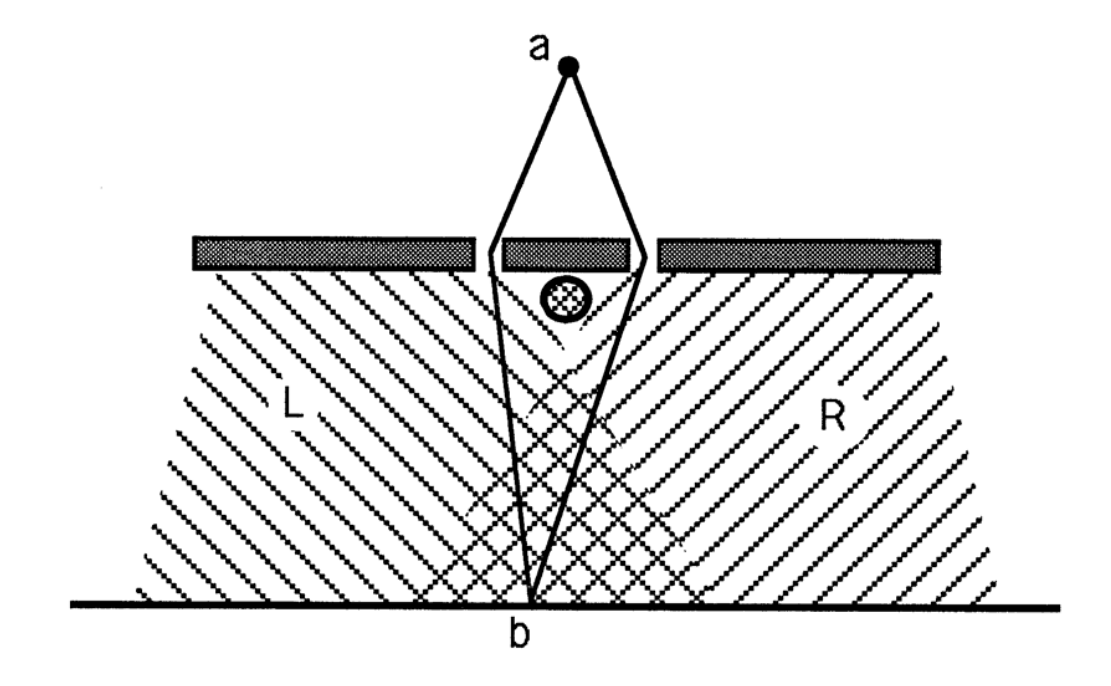
\includegraphics[height=4cm ,width=6.5cm]{QM/AB_effect.png}
	\caption{The Aharonov–Bohm experiment}
\end{figure}\\
Let $\Psi^{(0)}(\bm{x},t)$ be the solution of the Schrödinger equation and boundary conditions of this problem for the case in which the vector potential is everywhere zero. Now let us consider the case in which the magnetic field is non-zero inside the cylinder but zero outside of it. The vector potential $\bm{A}$ will not vanish everywhere in the exterior region, even though $\bm{B}=\bm{\nabla}\times\bm{A}=0$
outside of the cylinder. This follows by applying Stokes's theorem to any path surrounding the cylinder
\[\oint \bm{A}\cdot d\bm{x} = \int\int (\bm{\nabla}\times\bm{A})\cdot d\bm{S} = \int\int \bm{B}\cdot d\bm{S} = \Phi.\]
If the flux through the cylinder is not zero, then the vector potential must be nonzero on every path that encloses the cylinder. However in any simply connected region outside of the cylinder, it is possible to express the vector potential as the gradient of a scalar, from the zero potential solution by means of a gauge transformation, $\Psi = \Psi^{(0)}\exp(ie\Lambda)$.
\\ \\
In region L, which contains the slit on the left, the wave function can be written as $\Psi_{\mathrm{L}} = \Psi_{\mathrm{L}}\exp(ie\Lambda_1)$, where $\Psi_{\mathrm{L}}$ is the zero potential solution in region L, and $\Lambda_1(\bm{x},t) = \int \bm{A}\cdot d\bm{x}$, with the integral taken along a path within region L. A similar form can be written for the wave function in the region R, which contains the slit on the right.
At the point b, in the overlap of regions L and R, the wave function is a superposition of contributions from both slits. Hence we have
\[\Psi(\bm{b}) = \Psi_{\mathrm{L}}\exp(ie\Lambda_1) + \Psi_{\mathrm{R}}\exp(ie\Lambda_2).\]
The interference pattern depends $\exp(ie(\Lambda_1-\Lambda_2)) = \exp(ie\Phi)$. 
Therefore the interference pattern is sensitive to the magnetic flux inside of the cylinder, even though the particles never pass through the region in which the magnetic field is nonzero. 
The AB effect is a topological effect, in that the effect depends on the flux encircled by the paths available to the particle, even though the paths may never approach the region of the flux. 
\\ \\
At last, we conclude that in quantum theory, the potentials themselves are physically significant; however, they are subject to the requirement that all observable effects be invariant under gauge transformations.

\chapter{Angular Momentum}
\section{Eigenvalues of angular momentum operator}
Commutation relations among the angular momentum operators are
\[[J_i,J_j] = \epsilon_{ijk} J_k.\]
Angular momentum operators operators are self-adjoint. 
We first introduce the operator $J^2 \equiv J_x^2 + J_y^2 + J_z^2$. We can verify that $[J^2,\bm{J}] = 0$. Thus there exists a complete set of common eigenvectors of $J^2$ and any one component of $\bm{J}$. Particularly, we have the pair of eigenvalue equations
\[J^2 | \beta,m\rangle = \beta | \beta,m\rangle , \quad J_z | \beta,m\rangle = m | \beta,m\rangle.\]
Since
\[\langle \beta,m | J^2 | \beta,m \rangle = \langle \beta,m | J_x^2 | \beta,m \rangle + \langle \beta,m | J_y^2 | \beta,m \rangle + \langle \beta,m | J_z^2 | \beta,m \rangle,\]
we have $m^2 \leq \beta$. Thus for a fixed value of $\beta$ there must be maximum and minimum values for $m$.
Define
\[J_+ \equiv J_x + iJ_y , \quad J_- \equiv J_x - iJ_y.\]
We have commutation relations
\[[J_z,J_+] = J_+ , \quad [J_z,J_-] = -J_- , \quad [J_+,J_-] = 2J_z.\]
Thus
\[J_z J_+ | \beta,m\rangle = J_+(J_z + 1)| \beta,m\rangle = (m+1)J_+| \beta,m\rangle.\]
Therefore, either $J_+ | \beta,m\rangle$ is an eigenvector of $J_z$ with the raised eigenvalue $m+1$, or $J_+ | \beta,m\rangle = 0$. Now for fixed $\beta$ there is a maximum value of $m$, which we shall denote as $j$. It must be the case that
\[J_+ |\beta,j\rangle = 0.\]
Since
\[J_- J_+ = J^2 - J_z^2 - J_z,\]
it is obvious that $\beta = j(j+1)$. By similar method, we can show the minimum eigenvalue of $J_z$ for fixed $\beta$ satisfy that $\beta = k(k-1)$. Therefore, we have $k = -j$.
We have thus shown the existence of a set of eigenvectors corresponding to integer spaced $m$ values in the range $-j \leq m \leq j$. Since the difference between the maximum value $j$ and the minimum value $-j$ must be an integer, it follows that $j = \mbox{ integer} / 2$. Henceforth we shall adopt the common and more convenient notation of labeling the eigenvectors by $j$ instead of by $\beta$. Thus the vector that was previously denoted as $|\beta,m\rangle$ will now be denoted as $|j,m\rangle$. 
\\ \\
To find the matrix element of angular momentum operator, we notice that
\[\langle j,m| J_-J_+|j,m\rangle = j(j+1)-m(m+1).\]
Therefore, we can get
\[J_+ |j,m\rangle = \sqrt{(j+m+1)(j-m)} |j,m+1\rangle.\]
Similarly, we have
\[J_- |j,m\rangle = \sqrt{(j-m+1)(j+m)} |j,m-1\rangle.\]
The matrix element of $J_+$, $J_-$ and $J_z$ are
\[\langle j',m'| J_+ | j,m\rangle = \sqrt{(j+m+1)(j-m)} \delta_{jj'}\delta_{m',m+1}.\]
\[\langle j',m'| J_- | j,m\rangle = \sqrt{(j-m+1)(j+m)} \delta_{jj'}\delta_{m',m-1}.\]
\[\langle j',m'| J_z | j,m\rangle = m \delta_{jj'}\delta_{m',m}.\]

\section{Orbital Angular Momentum and Spin}
Let $\psi(\bm{x})$ be a one-component state function in coordinate representation. When it is subjected to a rotation it is transformed into
\[\bm{R}\psi(\bm{x}) = \psi(R^{-1}\bm{x}),\]
where $\bm{R}$ is the rotation operator generated by $\bm{R} = \exp(-i\bm{J}\cdot\bm{n}\theta)$. For a rotation through infinitesimal angle $\epsilon$ about the $z$ axis, we have
\[\bm{R}_z(\epsilon) \psi(x,y,z) = \psi(x+\epsilon y,y-\epsilon x,z) = \psi(x,y,x) + \epsilon (y \frac{\partial \psi}{\partial x} - x \frac{\partial \psi}{\partial y}).\]
On the other hand, 
\[\bm{R}_z(\epsilon) = I - i\epsilon J_z.\]
Thus we have $J_z = -i(x \partial_{y} - y \partial_{x})$.
This is just the $z$ component of the orbital angular momentum operator $L = \bm{X} \times \bm{P}$.
\\ \\
For a multicomponent state function, we have
\[\bm{R} \left( \begin{matrix} \psi_1(\bm{x}) \\ \psi_2(\bm{x}) \\  \vdots \end{matrix} \right) = D \left( \begin{matrix} \psi_1(R^{-1}\bm{x}) \\ \psi_2(R^{-1}\bm{x}) \\  \vdots \end{matrix} \right).\]
Thus the general form of the rotation operator will be
\[\bm{R}_{\bm{n}}(\theta) = e^{-i\bm{L}\cdot\bm{n}\theta}D_{\bm{n}}(\theta).\]
The two factors commute because the first acts only on the coordinate and the second acts only on the components of the column vector. The matrix $D$ must be unitary, and so it can be written as
\[D_{\bm{n}}(\theta) = e^{-i\bm{S}\cdot\bm{n}\theta}.\]
The angular momentum operator $\bm{J}$ has the form
\[\bm{J} = \bm{L} + \bm{S}\]
with $\bm{L} = \bm{X} \times \bm{P}$ and $[L_{\alpha},S_{\beta}] = 0$. In the particular representation used in this section, we have $\bm{L} = -i\bm{x}\times\bm{\nabla}$, and the components of $S$ are
discrete matrices. The operators $\bm{L}$ and $\bm{S}$ are called the orbital and spin parts of the angular momentum.

\subsubsection{Orbital angular momentum}
The form of the gradient operator in spherical coordinates is
\[\bm{\nabla} = \bm{e}_r \frac{\partial}{\partial r} + \bm{e}_{\theta} \frac{1}{r} \frac{\partial}{\partial \theta} + \bm{e}_{\phi} \frac{1}{r\sin\theta} \frac{\partial}{\partial \phi}.\]
The orbital angular momentum operator then has the form
\[\bm{L} = r\bm{e}_r \times (-i\bm{\nabla}) = (-i) \left[ \bm{e}_{\phi} \frac{\partial}{\partial \theta} - \bm{e}_{\theta} \frac{1}{\sin\theta} \frac{\partial}{\partial \phi} \right].\]
Therefore, we have
\[L_z = \bm{L}\cdot\bm{e}_z = -i\frac{\partial}{\partial \phi},\]
\[L^2 = \bm{L}\cdot\bm{L} = - \left [ \frac{1}{\sin\theta} \frac{\partial }{\partial \theta} (\sin\theta \frac{\partial }{\partial \theta}) + \frac{1}{\sin^2\theta} \frac{\partial^2}{\partial \phi^2}  \right ].\]
We must now solve the two coupled differential equations,
\[L_z Y_l^m(\theta,\phi) = m Y_l^m(\theta,\phi) , \quad L^2 Y_l^m(\theta,\phi) = l(l+1) Y_l^m(\theta,\phi).\]
Apart from normalization, we have $Y(\theta,\phi) = e^{im\phi}P_l^m(\cos\theta)$, where $P_l^m$ is the \href{https://en.wikipedia.org/wiki/Associated_Legendre_polynomials}{associated Legendre polynomials}. If we assume that the solution must be single-valued under rotation, then it will follow that $m$ must be an integer. If we further assume that it must be nonsingular at $\theta = 0$ and $\theta = \pi$, then from the standard theory of the Legendre equation it will follow that $l$ must be a nonnegative integer in the range $l \geq |m|$. The normalized solutions that result from these assumptions are the well-known \href{https://en.wikipedia.org/wiki/Spherical_harmonics}{spherical harmonics}
\[Y_l^m(\theta,\phi) = (-1)^{(m+|m|)/2} \left [\frac{(2l+1)(l-|m|)!}{4\pi(l+|m|)!}  \right ]^{1/2}e^{im\phi} P_l^{|m|}(\cos\theta).\]

\subsubsection{Spin}
A particular species of particle is characterized by a set of quantum numbers that includes the value of its spin $s$, it is often sufficient to treat the spin operators $\bm{S}$ as acting on the space of dimension
$2s+1$ that is spanned by the eigenvectors of for a fixed value of $s$. 
If $s= 1/2$, we have
\[S_x = \frac{1}{2} \left[ \begin{matrix} 0& 1\\ 1& 0\end{matrix} \right] , \quad S_y = \frac{1}{2} \left[ \begin{matrix} 0& -i\\ i& 0\end{matrix} \right] , \quad S_z = \frac{1}{2} \left[ \begin{matrix} 1& 0\\ 0& -1\end{matrix} \right].\]
The spin operator in direction $\bm{n} = (\sin\theta\cos\phi,\sin\theta\sin\phi,\cos\theta)$ is
\[\bm{S}_{n} = \frac{1}{2} \left[ \begin{matrix} \cos\theta& e^{-i\phi}\sin\theta\\ e^{i\phi}\sin\theta& -\cos\theta\end{matrix} \right].\]
The eigenvectors are
\[\left[ \begin{matrix} e^{-i\phi/2}\cos\frac{\theta}{2}\\ e^{i\phi/2}\sin\frac{\theta}{2} \end{matrix} \right] , \quad \left[ \begin{matrix} -e^{-i\phi/2}\sin\frac{\theta}{2}\\ e^{i\phi/2}\cos\frac{\theta}{2} \end{matrix} \right],\]
corresponding to eigenvalues $1/2$ and $-1/2$.
\\ \\
If $s= 1$, we have
\[S_x = \sqrt{\frac{1}{2}} \left[ \begin{matrix} 0& 1& 0\\ 1& 0& 1\\ 0& 1& 0\end{matrix} \right]  , \quad S_y = \sqrt{\frac{1}{2}} \left[ \begin{matrix} 0& -i& 0\\ i& 0& -i\\ 0& i& 0\end{matrix} \right] , \quad S_z = \left[ \begin{matrix} 1& 0& 0\\ 0& 0& 0\\ 0& 0& -1\end{matrix} \right].\]
The spin operator in direction $\bm{n} = (\sin\theta\cos\phi,\sin\theta\sin\phi,\cos\theta)$ is
\[\bm{S}_{n} =  \left[ \begin{matrix} \cos\theta& \sin\theta e^{-i\phi} \sqrt{\frac{1}{2}}& 0\\ \sin\theta e^{i\phi}\sqrt{\frac{1}{2}}& 0& \sin\theta e^{-i\phi} \sqrt{\frac{1}{2}}\\ 0& \sin\theta e^{i\phi} \sqrt{\frac{1}{2}}& -\cos\theta\end{matrix} \right].\]
The eigenvectors are
\[\left[ \begin{matrix} \frac{1}{2}(1+\cos\theta)e^{-i\phi}\\ \sqrt{\frac{1}{2}}\sin\theta \\ \frac{1}{2}(1-\cos\theta)e^{i\phi} \end{matrix} \right] , \quad \left[ \begin{matrix} -\sqrt{\frac{1}{2}}\sin\theta e^{-i\phi}\\ \cos\theta \\ \sqrt{\frac{1}{2}}\sin\theta e^{i\phi} \end{matrix} \right] , \quad \left[ \begin{matrix} \frac{1}{2}(1-\cos\theta)e^{-i\phi}\\ -\sqrt{\frac{1}{2}}\sin\theta \\ \frac{1}{2}(1+\cos\theta)e^{i\phi} \end{matrix} \right],\]
corresponding to eigenvalues $1$, $0$ and $-1$.

\section{Rotation operator}
Three parameters are required to describe an arbitrary rotation. A common parameterization is by the Euler angles. From the fixed system of axes $Oxyz$, a new rotated set of axes $Ox'y'z'$ is produced in three steps:
\begin{itemize}
\item Rotate through angle $\alpha$ about $Oz$, carrying $Oy$ into $Ou$.
\item Rotate through angle $\beta$ about $Ou$, carrying $Oz$ into $Oz'$.
\item Rotate through angle $\gamma$ about $Oz'$ , carrying $Ou$ into $Oy'$.
\end{itemize}
\begin{figure}[!h]
	\centering
	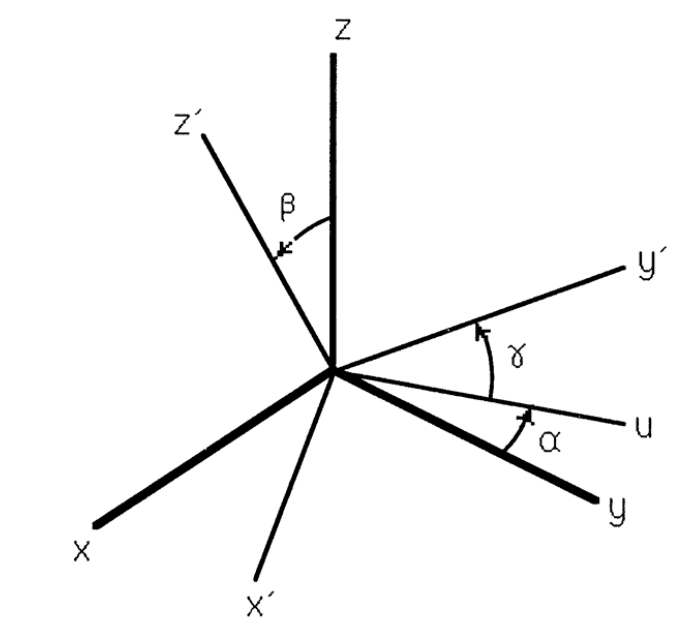
\includegraphics[height=4.5cm ,width=5cm]{QM/rotation.png}
	\caption{Euler angles}
\end{figure}
The net rotation is
\[\bm{R}(\alpha,\beta,\gamma) = \bm{R}_{z'}(\gamma) \bm{R}_{u}(\beta) \bm{R}_{z}(\alpha) = e^{-i\gamma J_{z'}} e^{-i\beta J_{u}} e^{-i\alpha J_{z}}.\]
Since $J_u = \bm{R}_z(\alpha) J_y \bm{R}_z(-\alpha)$, we have $\bm{R}_u(\beta) = \bm{R}_z(\alpha) \bm{R}_y(\beta) \bm{R}_z(-\alpha)$. Similarly, we can obtain $\bm{R}_{z'}(\gamma) = \bm{R}_{u}(\beta) \bm{R}_z(\gamma) \bm{R}_u(-\beta)$. Therefore, the rotation operator is
\[\bm{R}(\alpha,\beta,\gamma) = \bm{R}_{z}(\alpha) \bm{R}_{y}(\beta) \bm{R}_{z}(\gamma) = e^{-i\alpha J_{z}} e^{-i\beta J_{y}} e^{-i\gamma J_{z}}.\]
The matrix representation of the rotation operator in the basis $|j,m\rangle$
\[\langle j',m' | \bm{R}(\alpha,\beta,\gamma) | j,m \rangle = \delta_{jj'} D_{m'm}^{(j)}(\alpha,\beta,\gamma)\]
gives rise to the rotation matrices,
\[D_{m'm}^{(j)}(\alpha,\beta,\gamma) \equiv \langle j,m' | e^{-i\alpha J_{z}} e^{-i\beta J_{y}} e^{-i\gamma J_{z}} | j,m \rangle = e^{-i(\alpha m' + \gamma m)} d_{mm'}^{(j)}(\beta),\]
where
\[ d_{m'm}^{(j)}(\beta) \equiv \langle j,m' | e^{-i\beta J_{y}} | j,m \rangle.\]
For the case of $j = 1/2$, we have $J_y = \sigma_y/2$ and $\sigma_y^2 = I$. We can obtain
\[d^{(1/2)}(\beta) = \left[ \begin{matrix} \cos {\beta}/{2} & -\sin {\beta}/{2} \\ \cos {\beta}/{2}& \sin {\beta}/{2}\end{matrix} \right] .\]
Notice that this matrix is periodic in $\beta$ with period $4\pi$, but it changes sign when $2\pi$ is added to $\beta$. This double-valuedness under rotation by $2\pi$ is a characteristic of the full rotation matrix whenever $j$ is a half odd-integer. The matrix is single-valued under rotation by $2\pi$ whenever $j$ is an integer.
\\ \\
Rotation of angular momentum eigenvectors now can be written as
\[\bm{R}(\alpha,\beta,\gamma)|j,m\rangle = \sum_{m'} D_{m'm}^{(j)}(\alpha,\beta,\gamma) |j,m'\rangle.\]
When it comes to spherical harmonics, we have
\[Y_l^m(\theta',\phi') = \bm{R}^{-1}((\alpha,\beta,\gamma)) Y_l^m(\theta,\phi) = \sum_{m'} Y_{l}^{m'}(\theta,\phi) [D_{mm'}^{(j)}((\alpha,\beta,\gamma))]^*.\]
By putting $\beta = \gamma = 0$ we obtain
\[Y_l^m(\theta,\phi+\alpha) = \sum_{m'} Y_{l}^{m'}(\theta,\phi) [D_{mm'}^{(j)}((\alpha,0,0))]^* = e^{i\alpha m} Y_{l}^{m}(\theta,\phi).\]
Setting $\phi=0$ then yields
\[Y_l^m(\theta,\alpha) = e^{i\alpha m} Y_{l}^{m}(\theta,0).\]
Since the direction $\theta = 0$ is the polar axis, continuity of the spherical harmonic requires that $Y_l^m(0,\alpha)$ be independent of $\alpha$. Therefore we must
have $Y_l^m(0,0) = 0$ for $m \neq 0$, and so we can write
\[Y_{l}^{m}(0,0) = c_{l}\delta{m0}.\]
Then we have
\[Y_l^m(\theta,\phi) = \sum_{m'} Y_{l}^{m'}(0,0) [D_{mm'}^{(j)}((\phi,\theta,\gamma))]^* = c_l [D_{m0}^{(j)}((\phi,\theta,\gamma))]^*\]
for arbitrary $\gamma$, thus obtaining a simple relation between the spherical harmonics and the rotation matrices. Conventional normalization is obtained if we put
\[c_l = \left( \frac{2l+1}{4\pi} \right) ^{1/2}.\]
The operator for a rotation through $2\pi$ about an axis
along the unit vector $\bm{n}$ is $\bm{R}_{\bm{n}}(2\pi) = e^{-2\pi i\bm{n}\cdot\bm{J}}$. Its effect on the standard angular momentum eigenvectors is
\[\bm{R}_{\bm{n}}(2\pi) = (-1)^{2j}|j,m\rangle .\]
We assume a rotation through $2\pi$ as a trivial operation that leaves everything unchanged, i.e. all dynamical variables are invariant under $2\pi$ rotation:
\[\bm{R}(2\pi) A \bm{R}^{-1}(2\pi) = A,\]
where $A$ may represent any physical observable. 
\\ \\
The operator $\bm{R}_{2\pi}$ divides the vector space into two subspaces. A typical vector in the first subspace,
denoted as $|+\rangle$, has the property $\bm{R}(2\pi)|+\rangle = |+\rangle$, whereas a typical vector in the second subspace, denoted as $|-\rangle$, has the property $\bm{R}(2\pi)|-\rangle = -|-\rangle$. Now, if $A$ represents any physical observable, we have $\langle + | \bm{R}(2\pi) A| - \rangle = \langle + | A\bm{R}(2\pi)| - \rangle$, leading to 
\[\langle + | A | - \rangle = 0.\]
No physical observable can have nonvanishing matrix elements between states with integer angular momentum and states with half odd-integer angular momentum. This fact forms the basis of a superselection rule: There is no observable distinction among the state vectors of the form
\[|\Psi_{\omega}\rangle = |+\rangle + e^{i\omega}|-\rangle\]
for different values of the phase $\omega$.

\section{Addition of angular momentum}
Let us consider a two-component system, each component of which has angular momentum degrees of freedom. Basis vectors for the composite system can be formed from the basis vectors of the components by taking all binary products of a vector from each set
\[|j_1,j_2,m_1,m_2\rangle = |j_1,m_1\rangle ^{(1)} |j_2,m_2\rangle ^{(2)}.\]
These vectors are common eigenvectors of the four commutative operators $\bm{J}^{(1)}\cdot\bm{J}^{(1)}$, $\bm{J}^{(2)}\cdot\bm{J}^{(2)}$, $\bm{J}_z^{(1)}$, and $\bm{J}_z^{(2)}$.
It is often desirable to form eigenvectors of the total angular momentum operators, $\bm{J}\cdot\bm{J}$ and $\bm{J}_z$, where the total angular momentum vector operator is
\[\bm{J} = \bm{J}^{(1)}\otimes\bm{1} + \bm{1}\otimes\bm{J}^{(2)}.\]
This is useful when the system is invariant under rotation as a whole, but not under rotation of the two components separately. 
The eigenvectors of $\bm{J}\cdot\bm{J}$ and $\bm{J}_z$ may be denoted as $|\alpha, J, M \rangle$. It is easy to verify that the four operators $\bm{J}^{(1)}\cdot\bm{J}^{(1)}$, $\bm{J}^{(2)}\cdot\bm{J}^{(2)}$, $\bm{J}\cdot\bm{J}$ and $\bm{J}_z$ are mutually commutative, and hence they possess a complete set of common eigenvectors. 
Since the set of product vectors and the new set of total angular momentum eigenvectors are both eigenvectors of $\bm{J}^{(1)}\cdot\bm{J}^{(1)}$ and $\bm{J}^{(2)}\cdot\bm{J}^{(2)}$, the eigenvalues $j_1$ and $j_2$ will be constant in both sets. Therefore
we may confine our attention to the vector space of dimension $(2j_1+1)(2j_2+1)$ that is spanned by product vectors with fixed values of $j_1$ and $j_2$.
\\ \\
Now the $2J+1$ vectors $|\alpha, J, M \rangle$, with $M$ in the range $-J \leq M \leq J$, span an irreducible subspace.
Therefore if the vector $|\alpha, J, M \rangle$, for a particular value of $M$, can be constructed in the space under consideration, then so can the entire set of $2J+1$
such vectors with $M$ in the range $-J \leq M \leq J$.
For a particular value of $J$, it might be possible to construct one such set of vectors, two or more linearly independent sets, or none at all.
Let $N(J)$ denotes the number of independent sets that can be constructed. Let $n(M)$ be the degree of degeneracy, in this space, of the eigenvalue $M$ . The relation between these two quantities is
\[n(M) = \sum_{J \geq |M|} N(J),\]
and hence
\[N(J) = n(J) - n(J+1).\]
The product vectors $|j_1,m_1\rangle |j_2,m_2\rangle$ are eigenvectors of the operator $\bm{J}_z$, with eigenvalue $m_1+m_2$, and the degree of degeneracy $n(M)$ is equal to the number of pairs $(m_1,m_2)$ such that $M=m_1+m_2$.
\begin{figure}[!h]
	\centering
	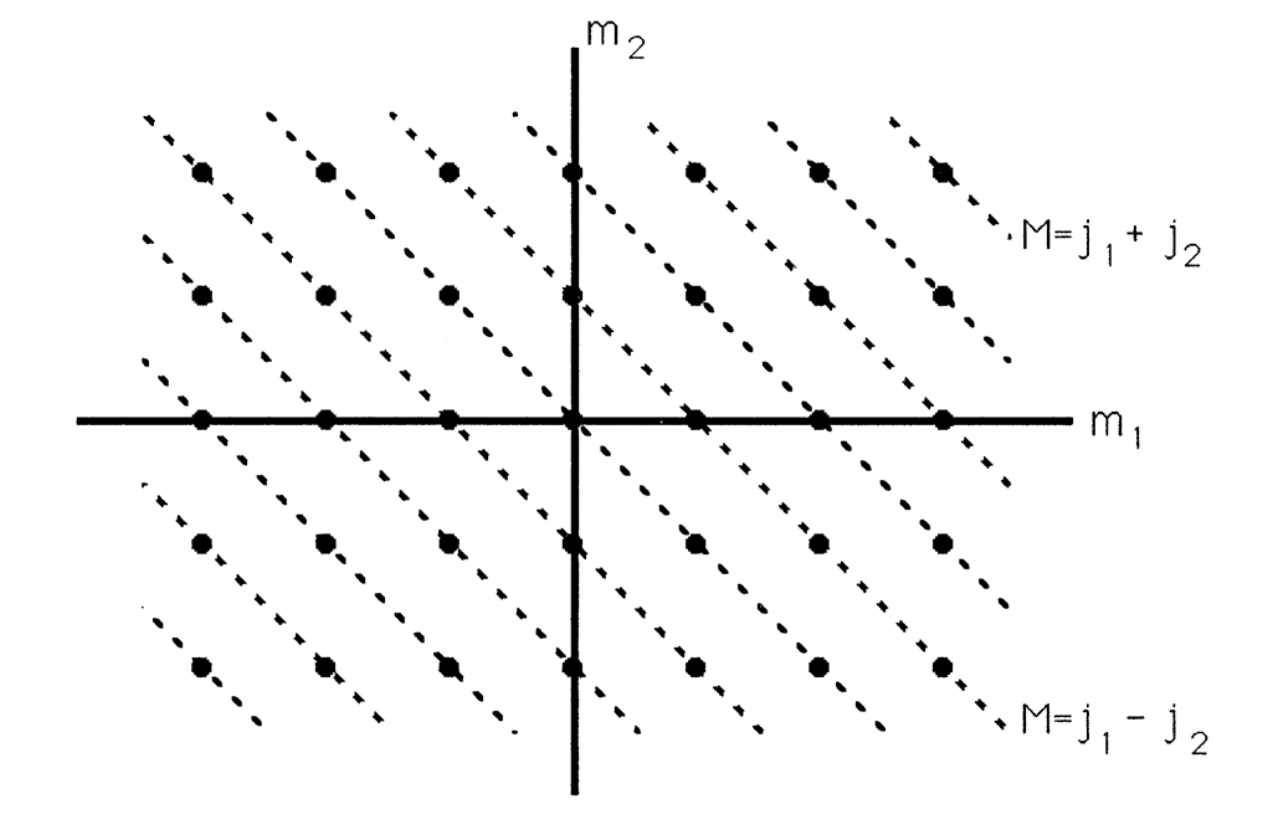
\includegraphics[height=4.14cm ,width=6.4cm]{QM/angular_momentum.png}
	\caption{Possible values of $M=m_1+m_2$ , illustrated for $j_1=3$, $j_2=2$}
\end{figure}
Therefore,
\[n(M)=\begin{cases} 0 , \quad |M| > j_1 + j_2\\ j_1+j_2+1-|M|, \quad |j_1-j_2| \leq M \leq |j_1+j_2|\\ 2j_{\mathrm{min}}+1 , \quad 0 \leq |M|\leq |j_1-j_2|\end{cases} .\]
It then follows that
\[N(J)=\begin{cases} 1 , \quad |j_1-j_2| \leq J \leq |j_1+j_2|\\ 0 , \quad \mbox{otherwise}\end{cases} .\]
It has turned out that $N(J)$ is never greater that $1$, and so the vectors $|\alpha, J, M \rangle$ can be uniquely labelled by the eigenvalues of the four operators $\bm{J}^{(1)}\cdot\bm{J}^{(1)}$, $\bm{J}^{(2)}\cdot\bm{J}^{(2)}$, $\bm{J}\cdot\bm{J}$ and $\bm{J}_z$. Henceforth these total angular momentum
eigenvectors will be denoted as $|j_1,j_2,J,M\rangle$. And we have the unitarity transformation 
\[|j_1,j_2,J,M\rangle = \sum_{m_1,m_2} |j_1,j_2,m_1,m_2\rangle \langle j_1,j_2,m_1,m_2 | j_1,j_2,J,M\rangle.\]
The coefficients of this transformation are called the Clebsch–Gordan coefficients, denoted as $(j_1,j_2,m_1,m_2|J,M)$.
The phases of the CG coefficients are not yet defined because of the indeterminacy of the relative phases of the vectors $|j_1,j_2,J,M\rangle$. For different values of $M$ but fixed $J$ we adopt the usual phase convention that led to
\[J_+ |j_1,j_2,J,M\rangle = \sqrt{(J+M+1)(J-M)} |j_1,j_2,J,M+1\rangle.\]
This leaves one arbitrary phase for each $J$ value, which we fix by requiring that $(j_1,j_2,j_1,J-j_1|J,J)$ be real and positive. It can be shown that all of the CG coefficients are now real.
We can also prove that CG coefficients vanishe unless following conditions are satisfied:
\begin{itemize}
\item $m_1+m_2=M$.
\item $|j_1-j_2| \leq J \leq |j_1+j_2|$.
\item $j_1+j_2+J =$ an integer.
\end{itemize}
It is possible to work out the values of the CG coefficients by successive application of the raising or lowering operator to
\[|j_1,j_2,J,M\rangle = \sum_{m_1,m_2} |j_1,j_2,m_1,m_2\rangle (j_1,j_2,m_1,m_2|J,M).\]
The details of the calculation can be found in section 7.7 of \emph{Quantum mechanics - a modern development(Leslie E. Ballentine)}. And we have \href{https://en.wikipedia.org/wiki/Table_of_Clebsch-Gordan_coefficients}{Table of CG coefficients} and \href{http://www.wolframalpha.com/input/?i=CG+coefficient}{Calculator of CG coefficients} on the internet. A special case of angular momentum addition is spin–orbit coupling of spin $1/2$ particles, and we list the corresponding CG coefficients $(l, 1/2, M-m_s, m_s|J,M)$ in the table 18.1.
\begin{table}[!th]
\centering
\begin{tabular}{|c|c|c|}
\hline
 & $J=l+1/2$ & $J=l-1/2$ \\
 \hline
 $m_s = 1/2$ & $\left[ \frac{l+M+1/2}{2l+1}\right ]^{1/2} $ & $-\left[ \frac{l-M+1/2}{2l+1}\right ]^{1/2} $ \\
 \hline
 $m_s = -1/2$ & $\left[ \frac{l-M+1/2}{2l+1}\right ]^{1/2} $ & $\left[ \frac{l+M+1/2}{2l+1}\right ]^{1/2} $ \\
\hline
\end{tabular}
\caption{Spin-Orbit coupling}
\end{table}
\\ \\
Now let us consider the relation between CG coefficients and rotation matrices. On the one hand, we have
\[\langle j_1,j_2,m_1,m_2 | \bm{R} | j_1,j_2,m'_1,m'_2\rangle = D_{m_1m'_1}^{(j_1)}(R) D_{m_2m'_2}^{(j_2)}(R).\]
On the other hand, we have
\begin{eqnarray}
&\phantom{=}& \langle j_1,j_2,m_1,m_2 | \bm{R} | j_1,j_2,m'_1,m'_2\rangle \nonumber \\
&=& \sum_{J,M,J',M'} (j_1,j_2,m_1,m_2|J,M) (j_1,j_2,m'_1,m'_2|J',M')  \langle j_1,j_2,J,M | \bm{R} | j_1,j_2,J',M'\rangle \nonumber \\
&=& \sum_{J,M,M'} (j_1,j_2,m_1,m_2|J,M) (j_1,j_2,m'_1,m'_2|J,M')D_{MM'}^{(J)}(R) .\nonumber
\end{eqnarray}
Therefore, we can get
\[D_{m_1m'_1}^{(j_1)}(R) D_{m_2m'_2}^{(j_2)}(R) = \sum_{J,M,M'} (j_1,j_2,m_1,m_2|J,M) (j_1,j_2,m'_1,m'_2|J,M')D_{MM'}^{(J)}(R).\]
It is called Clebsch-Gordan series.
\\ \\
Recall that
\[Y_l^m(\theta,\phi) =  \left( \frac{2l+1}{4\pi} \right) ^{1/2} [D_{m0}^{(j)}((\phi,\theta,0))]^* .\]
Thus we have
\[Y_{l_1}^{m_1}(\theta,\phi) Y_{l_2}^{m_2}(\theta,\phi) = \sum_{l,m} \sqrt{\frac{(2l_1+1)(2l_2+1)}{4\pi(2l+1)}} (l_1,l_2,m_1,m_2|l,m) (l_1,l_2,0,0|l,0) Y_l^m(\theta,\phi).\]
The orthogonal relation of spherical harmonics then would imply that
\[\int d\Omega Y_l^{m*}(\theta,\phi)Y_{l_1}^{m_1}(\theta,\phi) Y_{l_2}^{m_2}(\theta,\phi) = \sqrt{\frac{(2l_1+1)(2l_2+1)}{4\pi(2l+1)}} (l_1,l_2,m_1,m_2|l,m) (l_1,l_2,0,0|l,0).\]

\section{Tensor operators}
Suppose the state of the system is $|\psi\rangle$, then the state after rotation $R$ is $U(R)|\psi\rangle$, denoted as $|\psi'\rangle$. An operator $K$ is called scalar operator if and only if
\[\langle \psi' | K | \psi' \rangle = \langle \psi | K | \psi\rangle,\]
i.e.
\[U^{-1}(R)KU(R) = K.\]
Taking the case of infinitesimal rotation, we can derive that
\[[\bm{J},K] = 0.\]
A group of operators $\bm{V}$ is called vector operator if and only if
\[\langle \psi' | V_i | \psi' \rangle = R_{ii'} \langle \psi | V_{i'} | \psi\rangle,\]
i.e.
\[U^{-1}(R)V_{i}U(R) = \sum_{i'} R_{ii'} V_{i'}.\]
Taking the case of infinitesimal rotation, we can derive that
\[[J_i, V_j] = i\epsilon_{ijk}V_k.\]
If $\bm{V}$ and $\bm{W}$ are vector operators, we can prove that $\bm{V} \cdot \bm{W}$ is scalar operator and $\bm{V} \times \bm{W}$ is vector operator.
\\ \\
Similarly, tensor operators are defined as
\[U^{-1}(R) T_{ij\cdots k} U(R) = \sum_{i'\cdots} R_{ii'} R_{jj'} \cdots R_{kk'} T_{i'j'\cdots k'}.\]
Such a tensor is known as a Cartesian tensor.
The trouble with a Cartesian tensor is that it is reducible, i.e. it can be decomposed into objects that transform independently under rotations. For example, the trace of a tensor transform like a scalar under rotations. 
Thus we now define spherical tensor operators which are irreducible under rotations.  We define a spherical tensor operator of rank $k$ with $(2k+1)$ components as
\[U^{-1}(R) T^{(k)}_q U(R) = \sum_{q'=-k}^{k} [D^{(k)}_{qq'}(R)]^* T^{(k)}_{q'},\]
or equivalently
\[U(R) T^{(k)}_q U^{-1}(R) = \sum_{q'=-k}^{k} D^{(k)}_{q'q}(R) T^{(k)}_{q'},\]
where $D^{(k)}_{qq'}$ is the rotation matrix.
Taking the case of infinitesimal rotation, we can derive that
\[[J_{\pm},T^{(k)}_{q}] = \sqrt{(k \mp q)(k \pm q +1)} T^{(k)}_{q \pm 1},\]
\[[J_z, T^{(k)}_{q}] = q T^{(k)}_{q}.\]
For example, spherical components of a vector operator $\bm{V}$, 
\[V_{-1} = \frac{V_x - i V_y}{\sqrt{2}} , \quad V_0 = V_z , \quad V_{1} = -\frac{V_x + i V_y}{\sqrt{2}} ,\]
satisfy the commutation relation above, so they are spherical tensor of rank $1$. Generally, if $\bm{V}$ is a vector operator, then $Y_l^m(\bm{V})$ is a spherical tensor of ranks $l$.
\\ \\
Spherical tensors can be formed as products of other spherical  tensors, we have following theorem:
\\

\begin{newthem}
Let $X^{(k_1)}_{q_1}$ and $Z^{(k_2)}_{q_2}$ be irreducible spherical tensors of rank $k_1$ and $k_2$. Then
\[T^{(k)}_{q} = \sum_{q_1,q_2} (k_1,k_2,q_1,q_2|k,q) X^{(k_1)}_{q_1} Z^{(k_2)}_{q_2}\]
is an irreducible spherical tensor of rank $k$. 
\end{newthem}
\noindent
The proof can be found in section 3.10 of \emph{Modern Quantum Mechanics(J.J.Sakurai)}.

\begin{example}
suppose $\bm{V}$ and $\bm{U}$ are spherical tensor of rank $1$, then
\[T^{(0)}_{0} = \sqrt{\frac{1}{3}} (U_{-1}V_{1} + U_{1}V_{-1}-U_{0}U_{0}) = - \sqrt{\frac{1}{3}} (U_xV_x + U_yV_y + U_zV_z).\]
is a spherical tensor of rank $0$.
\end{example}

\noindent
Another important theorem on tensor operator is Wigner-Eckart theorem:\\

\begin{newthem}[Wigner-Eckart theorem]
The matrix elements of tensor operators with respect to angular-momentum eigenstates satisfy
\[\langle \tau',j',m'| T^{(k)}_{q}| \tau,j,m\rangle = (j,k,m,q|j',m') \frac{\langle \tau',j' || T^{(k)} || \tau,j\rangle}{\sqrt{2j+1}}.\]
where the double-bar matrix element is independent of $m$ and $m'$ and $q$.
\end{newthem}

\noindent
The proof can be found in section 3.10 of \emph{Modern Quantum Mechanics(J.J.Sakurai)}.
Therefore, for scaler operator $K$, we have
\[\langle \tau',j',m'| S| \tau,j,m\rangle = \delta_{jj'}\delta_{mm'} \frac{\langle \tau',j' || S || \tau,j\rangle}{\sqrt{2j+1}}.\]
For spherical tensor of rank $1$, we have
\[\langle \tau',j',m'| V_{q} | \tau,j,m\rangle = (j,1,m,q|j',m') \frac{\langle \tau',j' || V_q || \tau,j\rangle}{\sqrt{2j+1}}.\]
It would vanish unless
\[m'-m = q , \quad j'-j = 0,1,-1 , \quad j \mbox{ and } j' \mbox{ are not both  } 0.\]
For $j=j'$, Wigner-Eckart theorem - when applied to the vector operator- takes a particularly simple form. We can derive that
\[\langle \tau',j,m' | V_q | \tau, j ,m \rangle = \frac{\langle \tau',j,m | \bm{J}\cdot\bm{V} | \tau, j ,m \rangle}{j(j+1)} \langle j,m' | J_q | j ,m \rangle.\]

\begin{example}
The magnetic moment operator for an atom has the form
\[\bm{\mu} = \frac{-e}{2m_{\mathrm{e}} } (g_{\mathrm{L}}\bm{L} + g_{\mathrm{S}} \bm{S}).\]
The parameters $g_{\mathrm{L}}$ and $g_{\mathrm{S}}$ have approximately the
values $g_{\mathrm{L}} = 1$ and $g_{\mathrm{S}} = 2$. The former is an generalization of the magnetic moment we worked out in classical electrodynamics for a system of charged particles. The latter will be discussed in quantum field theory.
We define the effective Lande factor as
\[\langle \tau,J,M' | \bm{\mu} | \tau,J,M \rangle = \frac{-e}{2m_{\mathrm{e}} } g_{\mathrm{eff}} \langle J,M' | \bm{J} | J,M \rangle.\]
Then, we have
\[g_{\mathrm{eff}} = \frac{\langle \tau,J,M | g_{\mathrm{L}}\bm{L}\cdot\bm{J} + g_s \bm{S}\cdot\bm{J} | \tau,J,M \rangle}{J(J+1)} = 1 + \frac{J(J+1)- L(L+1) + S(S+1)}{2J(J+1)}.\]
\end{example}

\section{Spherical potential well}
The stationary states of a particle in the spherical potential well are determined by
\[-\frac{1}{2m}\nabla^2 \Psi  + W(r) \Psi = E\Psi .\]
In spherical coordinates, 
\[\nabla^2 = \frac{1}{r^2} \frac{\partial}{\partial r} \left [ r^2\frac{\partial}{\partial r} \right ] + \frac{1}{r^2\sin\theta} \frac{\partial}{\partial \theta} \left [\sin\theta \frac{\partial}{\partial \theta} \right ] + \frac{1}{r^2\sin^2\theta} \frac{\partial^2}{\partial\phi^2}.\]
Therefore, the eigenvalue equation becomes
\[-\frac{1}{2m} \frac{1}{r^2} \frac{\partial}{\partial r} \left [ r^2\frac{\partial \Psi}{\partial r}\right ]  + \frac{L^2}{2mr^2} \Psi + W(r)\Psi = E\Psi.\]
Suppose the eigenfunctions have the factored form
\[\Psi(r,\theta,\phi) = Y_l^m(\theta,\phi) \frac{u(r)}{r}.\]
The radial function then satisfies the equation
\[-\frac{1}{2m} \frac{d^2 u(r)}{dr^2} + \left[ \frac{l(l+1)}{2mr^2} + W(r)\right]u(r) = Eu(r).\]
The radial function must satisfy the boundary condition $u(0) = 0$ since $\Psi(r,\theta,\phi)$ would otherwise have an $r^{-1}$ singularity at the origin. The normalization $\langle \Psi | \Psi \rangle = 1$ implies that
\[\int_0^{\infty} = |u(r)|^2 dr = 1.\]

\subsubsection{The hydrogen atom}
The hydrogen atom is a two-particle system consisting of an electron and a proton. The Hamiltonian is
\[H = \frac{P_{\mathrm{e}}^2}{2m_{\mathrm{e}}} + \frac{P_{\mathrm{p}}^2}{2m_{\mathrm{p}}} - \frac{e^2}{4\pi|\bm{Q}_{\mathrm{e}}-\bm{Q}_{\mathrm{p}}|}.\]
We take as independent variables the center of mass and relative coordinates of the particles
\[\bm{Q}_{\mathrm{c}} = \frac{m_{\mathrm{e}}\bm{Q}_{\mathrm{e}} + m_{\mathrm{p}}\bm{Q}_{\mathrm{p}}}{m_{\mathrm{e}}+m_{\mathrm{p}}} , \quad \bm{Q}_{\mathrm{r}} = \bm{Q}_{\mathrm{e}}-\bm{Q}_{\mathrm{p}}.\]
The corresponding momentum operators are
\[\bm{P}_{\mathrm{c}} = \bm{P}_{\mathrm{e}} + \bm{P}_{\mathrm{p}} , \quad \bm{P}_{\mathrm{r}} = \frac{m_{\mathrm{p}}\bm{P}_{\mathrm{e}}-m_{\mathrm{e}}\bm{P}_{\mathrm{p}}}{m_{\mathrm{e}} + m_{\mathrm{p}}}.\]
We can verify that
\[[Q_{\mathrm{c}\alpha},P_{\mathrm{c}\beta}] = [Q_{\mathrm{r}\alpha},P_{\mathrm{r}\beta}] = i\delta_{\alpha\beta} , \quad [Q_{\mathrm{c}\alpha},P_{\mathrm{r}\beta}] = [Q_{\mathrm{r}\alpha},P_{\mathrm{c}\beta}] = 0.\]
The Hamiltonian becomes
\[H = \frac{P_{\mathrm{c}}^2}{2(m_{\mathrm{e}}+m_{\mathrm{p}})} + \frac{P_{\mathrm{r}}^2}{2\mu} - \frac{e^2}{4\pi|\bm{Q}_{\mathrm{r}}|},\]
where $\mu$ is called the reduced mass, and is defined by $\mu \equiv {m_{\mathrm{e}}m_{\mathrm{p}}}/({m_{\mathrm{e}}+m_{\mathrm{p}}})$.
The center of mass behaves as a free particle, and its
motion is not coupled to the relative coordinate. We shall confine our attention to the internal degrees of freedom described by the relative coordinate $\bm{Q}_{\mathrm{r}}$. The energy eigenvalue equation in coordinate representation is
\[-\frac{1}{2\mu}\nabla^2 \Psi(\bm{r})  -\frac{e^2}{4\pi r} \Psi(\bm{r}) = E\Psi(\bm{r}).\]
Suppose $\Psi(r,\theta,\phi) = Y_l^m(\theta,\phi) \frac{u(r)}{r}$, we have
\[-\frac{1}{2\mu} \frac{d^2 u(r)}{dr^2} + \left[ \frac{l(l+1)}{2\mu r^2} - \frac{e^2}{4\pi r}\right]u(r) = Eu(r).\]
Define
\[\rho \equiv \alpha r , \quad \alpha \equiv \sqrt{8\mu|E|} , \quad \lambda \equiv \frac{e^2}{4\pi} \sqrt{\frac{\mu}{2|E|}}.\]
We have
\[\frac{d^2 u}{d\rho^2} + \left[ -\frac{1}{4} + \frac{\lambda}{\rho} - \frac{l(l+1)}{\rho^2} \right] u = 0.\]
As $\rho \to \infty$, we have $u \sim e^{-\rho/2}$. And as $\rho \to 0$, we have $u \sim \rho^{l+1}$. Therefore, we can suppose
\[u(\rho) = \rho^{l+1} e^{-\rho/2} v(\rho).\]
And we can get
\[\rho \frac{d^2 v}{d\rho^2} + (2l+2-\rho)\frac{dv}{d\rho} + (\lambda-l-1)v = 0.\]
It is the so-called \href{http://mathworld.wolfram.com/ConfluentHypergeometricDifferentialEquation.html}{Confluent Hypergeometric Differential Equation}.
When $\lambda - 1- l = n_r$, we have regular solutions. Solutions are \href{https://en.wikipedia.org/wiki/Laguerre_polynomials#Generalized_Laguerre_polynomials}{Associated Laguerre Polynomial}, and will be denoted as $L_{n-l-1}^{2l+1}(\rho) (n=n_r+l+1)$. The energy levels are
\[E_n = -\frac{\mu e^4}{32\pi^2 n^2}.\]
The degeneracy of an eigenvalue $E_n$ is
\[\sum_{l=0}^{n-1} (2l+1) = n^2.\]
\begin{note}
The degeneracy of an energy level of a hydrogen atom is greater than this by a factor of $4$, which arises from the two-fold orientational degeneracies of the electron and proton spin states. This four-fold degeneracy is modified by the hyperfine interaction between the magnetic moments of the electron and the proton.
\end{note}
\noindent
The orthonormal energy eigenfunctions for the hydrogen atom are
\[\Psi_{nlm}(r,\theta,\phi) =  \left[ \frac{4(n-l-1)!}{(na_0)^3 n[(n+l)!]^3} \right]^{\frac{1}{2}} \rho^l L_{n-l-1}^{2l+1}(\rho) e^{-\rho/2} Y_l^m (\theta,\phi),\]
where $\rho = \alpha r = {2r}/{na_0}$, and $a_0 \equiv {4\pi}/{\mu e^2}$ is a characteristic length for the
atom, known as the Bohr radius.The ground state wave
function is
\[\Psi_{000} = (\pi a_0^3)^{-\frac{1}{2}} e^{-\frac{r}{a_0}}.\]
A measure of the spatial extent of the bound states of hydrogen is given by the averages of various powers of the distance $r$:
\begin{eqnarray}
\langle r \rangle &=& n^2a_0 \left \{ 1 + \frac{1}{2} \left [ 1 - \frac{l(l+1)}{n^2} \right] \right\} ,\nonumber \\
\langle r^2 \rangle &=& n^4a_0^2 \left \{ 1 + \frac{3}{2} \left [ 1 - \frac{l(l+1)-1/3}{n^2} \right] \right\}, \nonumber \\
\left\langle \frac{1}{r} \right\rangle &=& \frac{1}{n^2 a_0}. \nonumber
\end{eqnarray}

\chapter{Discrete Symmetries}
\section{Space inversion}
The space inversion transformation is $\bm{x} \to -\bm{x}$. The corresponding operator on state vector space is usually called the parity operator. It will be denoted by $P$. By definition, the parity operator reverses the signs of the position operator and the momentum operator
\[P^{-1}\bm{X}P = -\bm{X} , \quad P^{-1}\bm{P}P = -\bm{P}.\]
It follows that the orbital angular momentum, $\bm{L} = \bm{X}\times\bm{P}$, is unchanged by the parity transformation. This property is extended, by definition, to any angular momentum operator,
\[P^{-1}\bm{J}P = \bm{J}.\]
We can verify that $P$ must be linear by applying space inversion to the commutation relation $[X_i,P_i] = i$. Therefore the parity operator is a unitary operator rather than an anti-unitary operator. Since two consecutive space inversions produce no change at all, it follows that the states described by $|\psi\rangle$ and by $P^2|\psi\rangle$ must be the same. Thus the
operator $P^2$ can differ from the identity operator by at most a phase factor. This phase factor is left arbitrary. It is most convenient to choose that phase factor to be unity, and hence we have
\[P = P^{-1} = P^{\dagger}.\]
Further more, we can derive that
\[P|\bm{x}\rangle = |-\bm{x}\rangle.\]
Thus the effect of $P$ on a wave function is
\[P\psi(\bm{x}) \equiv \langle \bm{x} | P | \psi\rangle = \langle -\bm{x} | \psi\rangle = \psi(-\bm{x}).\]
From the fact the $P^2=1$, it follows that $P$ has eigenvalues $\pm 1$. Any even function, $\psi_{\mathrm{e}}(\bm{x}) = \psi_{\mathrm{e}}(-\bm{x})$, is an eigenfunction on $P$ with eigenvalue $1$, and any odd function, $\psi_{\mathrm{o}}(\bm{x}) = -\psi_{\mathrm{o}}(-\bm{x})$, is an eigenfunction of $P$ with eigenvalue $-1$.
A function corresponding to parity $+1$ is also said to be of even parity, and a function corresponding to parity $-1$ is said to be of odd parity.
If the parity of operator $K$ is $p$, i.e. 
\[PKP = pK,\] 
and the parity of the state $|\psi_1\rangle$ and $|\psi_2\rangle$ are $p_1$ and $p_2$ respectively, then we can prove that 
\[\langle \psi_1 | K | \psi_2 \rangle \]
vanishes unless $p = p_1 p_2$.

\begin{example}
Under space inversion, $\bm{x} \to -\bm{x}$, the spherical harmonic undergoes the transformation
\[Y_l^m(\theta,\phi) \to Y_l^m(\pi-\theta,\phi+\pi) = (-1)^l Y_l^m(\theta,\phi).\]
Hence the single particle orbital angular momentum eigenvector $|l,m\rangle$ is also an eigenvector of parity, with parity $(-1)^l$.
A total orbital angular momentum eigenvector for a two-
electron atom is of the form
\[|l_1,l_2,L,M\rangle = \sum_{m_1,m_2}  \langle l_1,l_2,m_1,m_2 | l_1,l_2,L,M\rangle |l_1,m_1\rangle \otimes |l_2,m_2\rangle.\]
It is apparent that
\[P|l_1,l_2,L,M\rangle = (-1)^{l_1+l_2}| l_1,l_2,L,M\rangle ,\]
and that $(-1)^{l_1+l_2} \neq (-1)^{L}$ . Thus we see that, in general, the parity of an angular momentum state is not determined by its total angular momentum.
\end{example}

\noindent
If the parity operator $P$ commutes with the Hamiltonian $H$, then parity eigenvalue $\pm 1$ is a conserved quantity. In that case an even parity state can never acquire an odd parity component, and an odd parity state can never acquire an even parity component.
If $|\psi(t)\rangle$ is a physical process of the system with Hamiltonian $H$, then we have Schrödinger equation 
\[H|\psi\rangle = i\frac{\partial |\psi\rangle }{\partial t}.\]
If $PH = HP$, we can verify that
\[H P|\psi\rangle = i\frac{\partial P |\psi\rangle }{\partial t}.\]
Therefore, the space inversion of $|\psi(t)\rangle$, $P|\psi(t)\rangle$, can also be a possible physical process of the system.
Experiments have shown that parity in $\beta$ decay is not conserved.

\section{Time reversal}
The effect of the time reversal operator $T$ is to reverse the linear and angular momentum while leaving the position unchanged. Thus we require, by definition,
\[T^{-1}\bm{X}T = \bm{X} , \quad T^{-1}\bm{P}T = -\bm{P} , \quad T^{-1}\bm{J}T = -\bm{J}.\]
We can verify that $T$ must be anti-linear by applying space inversion to the commutation relation $[X_i,P_i] = i$. Therefore the parity operator is an anti-unitary operator.
The time evolution of a system satisfies Schrödinger equation
\[H|\psi(t)\rangle = i\frac{\partial |\psi(t)\rangle }{\partial t}.\]
Suppose that $TH=HT$, we can derive that
\[HT|\psi(t)\rangle = -i\frac{\partial T|\psi(t)\rangle }{\partial t},\]
i.e.
\[HT|\psi(-t)\rangle = i\frac{\partial T|\psi(-t)\rangle }{\partial t}.\]
$T|\psi(-t)\rangle$ is also a possible physical process of the system.
\\ \\
In coordinate representation the Schrödinger equation takes the form
\[ \left[ -\frac{1}{2m}\nabla^2 + W(\bm{x}) \right] \psi(\bm{x},t) = i\frac{\partial \psi(\bm{x},t)}{\partial t}.\]
Its complex conjugate is
\[ \left[ -\frac{1}{2m}\nabla^2 + W^*(\bm{x}) \right] \psi^*(\bm{x},t) = -i\frac{\partial \psi^*(\bm{x},t)}{\partial t}.\]
The condition for the Hamiltonian to be invariant under complex conjugation is that the potential be real: $W=W^*$. In that case it is apparent that if $\psi(\bm{x},-t)$ is a solution then so is  $\psi^*(\bm{x},t)$. This suggests that we may identify the time reversal operator with the complex conjugation operator in this representation,
\[T = K_0,\]
where, by definition, $K_0\psi(\bm{x},t) = \psi^*(\bm{x},t)$. In this case $T$ is its own inverse. 
The formal expression for an arbitrary vector in coordinate representation is $|\psi\rangle = \int \psi(\bm{x})|\bm{x}\rangle d^3 \bm{x}$, where the basis vector $|\bm{x}\rangle$ is an eigenvector of the position operator. Since $T$ is equal to the complex conjugation operator, its effect is simply $T|\psi\rangle = \int \psi^*(\bm{x})|\bm{x}\rangle d^3 \bm{x}$, with $T|\bm{x}\rangle = |\bm{x}\rangle$.
\\ \\
In momentum representation, an arbitrary vector can be written as
\[|\psi\rangle = \int \psi(\bm{p})|\bm{p}\rangle d^3 \bm{p}.\]
Since
\[T|\bm{p}\rangle = \int \langle \bm{x} | \bm{p}\rangle^* |
\bm{x}\rangle d^3 \bm{x} = |-\bm{p}\rangle,\]
we have
\[T|\psi\rangle = \int \psi^*(\bm{p})|-\bm{p}\rangle d^3 \bm{p} = \int \psi^*(\bm{-p})|\bm{p}\rangle d^3 \bm{p}.\]
The time reversal operator must reverse the angular momentum. For spin operator, we have
\[T^{-1}\bm{S}T = -\bm{S}.\]
In the standard representation of the spin operators, $S_x$ and $S_z$ are real, while $S_y$ is imaginary. The time reversal operator $T$ cannot be equal to the complex conjugation operator $K_0$ in this representation, since the effect of the latter is
\[K_0S_xK_0 = S_x , \quad K_0S_yK_0 = -S_y , \quad K_0S_zK_0 = S_z.\]
Let us write the time reversal operator as $T=YK_0$, where $Y$ is a linear operator. $Y$ must have the following properties:
\[Y^{-1}S_xY = -S_x , \quad Y^{-1}S_yY = S_y , \quad Y^{-1}S_zY = -S_z.\]
And $Y$ must operate only on the spin degrees of freedom. A reasonable choice is that $Y = e^{-i\pi S_y}$, whose effect is
to rotate spin (and only spin) through the angle $\pi$ about the $y$ axis. Therefore the explicit form of the time reversal in this representation is
\[T = e^{-i\pi S_y}K_0.\]
Two successive applications of the time reversal transformation, must leave the physical situation unchanged. Therefore
\[T^2|\Psi\rangle = c|\Psi\rangle,\]
where $|c|=1$. And we have
\[T^2(T|\Psi\rangle) = T(T^2|\Psi\rangle) = T(c|\Psi\rangle) = c^* T|\Psi\rangle.\]
Thus 
\[T^2(|\Psi\rangle + T|\Psi\rangle) = c|\Psi\rangle + c^* T|\Psi\rangle = c'(|\Psi\rangle + T|\Psi\rangle).\]
And we can determine that $c' = c^* = c$. Thus we must have $c = \pm 1$, i.e.
\[T^2|\Psi\rangle = \pm |\Psi\rangle.\]
In the particularly representation, we have
\[T^2 = e^{-i\pi S_y}K_0 e^{-i\pi S_y}K_0 = e^{-i2\pi S_y}.\]
This may equivalently be written as
\[T^2 = e^{-i2\pi J_y},\]
since $e^{-i2\pi L_y} = I$. Thus we have an identity
\[T^2 = R(2\pi).\]

\subsubsection{Kramer's theorem}
Let us consider the energy eigenvalue equation, $H|\Psi\rangle = E|\Psi\rangle$, for a time-reversal-invariant Hamiltonian, $TH=HT$. 
Then $HT|\Psi\rangle =  TH|\Psi\rangle = ET|\Psi\rangle$, and so
both $|\Psi\rangle$ and $T|\Psi\rangle$ are eigenvectors with energy eigenvalue $E$. 
There are two possibilities: 
(a) $|\Psi\rangle$and $T|\Psi\rangle$ are linearly dependent, and so describe the same state.
(b) $|\Psi\rangle$and $T|\Psi\rangle$ are linearly independent,
and so describe two degenerate states.
\\ \\
Suppose that (a) is true, in which case we must have $T|\Psi\rangle = a|\Psi\rangle$ with $|a|=1$. A second application of T yields $T^2|\Psi\rangle = |\Psi\rangle$. 
Thus for those states that satisfy $T^2|\Psi\rangle = -|\Psi\rangle$ it is necessarily true that $|\Psi\rangle$and $T|\Psi\rangle$ are linearly independent, degenerate states. This result is known as Kramer's theorem: any
system for which $T^2|\Psi\rangle = -|\Psi\rangle$ has only degenerate energy levels.
\chapter{Approximation Method}
\section{Time independent perturbation theory}
\subsection{Brillouin-Wigner perturbation theory}
We consider an unperturbed Hamiltonian $H_0$ with eigenvalues $\epsilon_k$ and eigenstates $|k\alpha\rangle$, where $\alpha$ is an index introduced to resolve degeneracies, so that
\[H_0 |k\alpha\rangle = \epsilon_k |k\alpha\rangle.\]
We pick one of these levels $\epsilon_n$ for study, so the index $n$ will be fixed for the following discussion. We denote the eigenspace of the unperturbed system corresponding to eigenvalue  $\epsilon_n$ by $\mathcal{H}$, so that the unperturbed eigenkets
$\{ |n\alpha\rangle, \alpha = 1,2,\cdots\}$ form a basis in this space.\\
We take the perturbed Hamiltonian to be $H = H_0 + \lambda H_1$, where $\lambda$ is a formal expansion parameter that we allow to vary between $0$ and $1$ to interpolate between the unperturbed and perturbed system. When the perturbation is turned on, the unperturbed energy level $\epsilon_n$ may split and shift. We denote one of the exact energy levels that grows out of $\epsilon_n$ by $E$. We let $|\psi\rangle$ be an exact energy eigenket corresponding to energy $E$, so that
\[H|\psi\rangle = (H_0 + \lambda H_1)|\psi\rangle = E|\psi\rangle.\]
Both $E$ and $|\psi\rangle$ are understood to be functions of $\lambda$; as $\lambda \to 0$, $E$ approaches $\epsilon_n$ and $|\psi\rangle$ approaches some state lying in $\mathcal{H}_n$. We break the Hilbert space into the subspace $\mathcal{H}_n$ and its orthogonal complement which we denote by $\mathcal{H}_n^{\bot}$. The components of $|\psi\rangle$ parallel and perpendicular to $\mathcal{H}_n$ are conveniently expressed in terms of the projector $P$ onto the subspace $\mathcal{H}_n$ and the orthogonal projector $Q$, defined by
\[P \equiv \sum_{\alpha} |n\alpha\rangle \langle n\alpha| , \quad Q \equiv \sum_{k \neq n,\alpha} |k\alpha\rangle \langle k\alpha|.\]
These projectors satisfy
\[P^2=P , \quad Q^2=Q , \quad PQ=QP=0 , \quad P+Q=I , \quad [P,H_0]=[Q,H_0]=0.\]
The component $P|\psi\rangle$ is a linear combination of the known unperturbed eigenstates $\{ |n\alpha\rangle, \alpha = 1,2,\cdots\}$, and is easily characterized. 
The orthogonal component $Q|\psi\rangle$ is harder to find. It turns out it is possible to write a neat power series expansion for this solution. Firstly, we have
\[(E-H_0)|\psi\rangle = \lambda H_1 |\psi\rangle.\]
Now we define a new operator $R$
\[R \equiv \sum_{k \neq n,\alpha} \frac{|k\alpha\rangle \langle k\alpha|}{E-\epsilon_k}.\]
\begin{note}
If there are other unperturbed energy levels $\epsilon_k$ lying close to $\epsilon_n$, then the perturbation could push
the exact energy $E$ near to or past some of these other levels, and then other small denominators would make $R$ ill defined.
This will certainly happen if the perturbation is large enough. For the time being we will assume this does not happen, so that $R$ is free of small denominators. When this is not the case we shall refer to ``nearly degenerate perturbation theory'', which is discussed later.
\end{note}
\noindent
The operator $R$ satisfies
\[PR=RP=0 , \quad QR=RQ=R , \quad R(E-H_0) = (E-H_0)R = Q.\]
Then we have
\[R(E-H_0)|\psi\rangle = Q|\psi\rangle = \lambda RH_1 |\psi\rangle \]
and
\[|\psi\rangle = P|\psi\rangle + \lambda R H_1 |\psi\rangle.\]
$|\psi\rangle$ can be solved as a series of $P|\psi\rangle$:
\[|\psi\rangle = \frac{1}{1-\lambda RH_1} P|\psi\rangle = P|\psi\rangle + \lambda RH_1P|\psi\rangle + \lambda^2 RH_1RH_1 P|\psi\rangle + \cdots.\]

\subsection{Nondegenerate perturbation theory}
In nondegenerate perturbation theory the level $\epsilon_n$ of $H_0$ is nondegenerate. Then the index $\alpha$ is not needed for the level $\epsilon_n$, and we can write simply $|n\rangle$ for the corresponding eigenstate. We assume that $P|\psi\rangle$ is normalized rather than $|\psi\rangle$ so that
\[P|\psi\rangle  = |n\rangle.\]
With this normalization convention, we have
\[\langle n | \psi \rangle = 1.\]
Now the series becomes
\[|\psi\rangle = |n\rangle + \lambda \sum_{k\neq n,\alpha} |k\alpha\rangle \frac{\langle k\alpha | H_1 | n \rangle}{E-\epsilon_k} + \lambda^2 \sum_{k\neq n,\alpha} \sum_{k'\neq n,\alpha'} |k\alpha\rangle \frac{\langle k\alpha | H_1 | k'\alpha' \rangle \langle k'\alpha' | H_1 | n \rangle}{(E-\epsilon_k)(E-\epsilon_{k'})}.\]
To find an equation for $E$, we have
\[\langle n | E-H_0 | \psi\rangle = E-\epsilon_n = \lambda \langle n | H_1 | \psi\rangle.\]
Then we can get
\begin{eqnarray}
E &=& \epsilon_n + \lambda \langle n | H_1 | n\rangle + \lambda^2 \langle n | H_1RH_1 | n\rangle + \lambda^3 \langle n | H_1RH_1RH_1 | n\rangle + \cdots \nonumber \\
&=& \epsilon_n 
+ \lambda \langle n | H_1|n\rangle 
+ \lambda^2 \sum_{k\neq n,\alpha}  \frac{ \langle n | H_1|k\alpha\rangle \langle k\alpha | H_1 | n \rangle}{E-\epsilon_k} \nonumber \\
&+& \lambda^3 \sum_{k\neq n,\alpha} \sum_{k'\neq n,\alpha'} \frac{\langle n | H_1 |k\alpha\rangle \langle k\alpha | H_1 | k'\alpha' \rangle \langle k'\alpha' | H_1 | n \rangle}{(E-\epsilon_k)(E-\epsilon_{k'})} + \cdots \nonumber
\end{eqnarray}
It is easy to get $E$ up to $O(\lambda^3)$,
\[E = \epsilon_n  + \lambda \langle n | H_1|n\rangle  + \lambda^2 \sum_{k\neq n,\alpha}  \frac{\lambda \langle n | H_1|k\alpha\rangle \langle k\alpha | H_1 | n \rangle}{\epsilon_n-\epsilon_k} + O(\lambda^3),\]
and $|\psi\rangle$ up to $O(\lambda^2)$,
\[|\psi\rangle = |n\rangle + \lambda \sum_{k\neq n,\alpha} |k\alpha\rangle \frac{\langle k\alpha | H_1 | n \rangle}{\epsilon_n-\epsilon_k} + O(\lambda^2).\]
\href{https://en.wikipedia.org/wiki/Perturbation_theory_(quantum_mechanics)#Second-order_and_higher_corrections}{Higher corrections} can be found on the internet.

\subsection{Degenerate perturbation theory}
In the case that the unperturbed energy level $\epsilon_n$ is degenerate, we have
\[P|\psi\rangle = \sum_{\alpha} |n\alpha\rangle c_{\alpha}\]
and
\[\langle n\alpha | P |\psi\rangle = \langle n\alpha  |\psi\rangle = c_{\alpha}.\]
Then we can obtain an equation for the $c_{\alpha}$,
\[\langle n\alpha | E-H_0 | \psi\rangle = c_{\alpha}(E-\epsilon_n) = \lambda \langle n\alpha | H_1 | \psi\rangle,\]
i.e.
\begin{eqnarray}
(E-\epsilon_{n})c_{\alpha} &=& \lambda \sum_{\beta} \langle n\alpha | H_1 | n\beta\rangle c_{\beta} + \lambda^2 \sum_{\beta} \langle n\alpha | H_1RH_1 | n\beta\rangle c_{\beta} + \cdots \\
&=& \lambda \sum_{\beta} \langle n\alpha | H_1 | n\beta\rangle c_{\beta}
+ \lambda^2 \sum_{\beta} \sum_{k\neq n,\gamma}  \frac{\lambda \langle n\alpha | H_1|k\gamma\rangle \langle k\gamma | H_1 | n\beta \rangle}{E-\epsilon_k}c_{\beta} + \cdots \nonumber
\end{eqnarray}
This equation must be solved simultaneously for the eigenvalues $E$ and the unknown expansion coefficients $c_{\alpha}$.
If we truncate the series at first order, we see that the corrections $E-\epsilon_{n}$ to the energies are determined as the eigenvalues of the matrix $\langle n\alpha | H_1 | n\beta\rangle$, and the coefficients $c_{\alpha}$ are the corresponding eigenvectors.
This determines the energies to first order, but the coefficients $c_{\alpha}$ only to zeroth order. Then $P|\psi\rangle$ becomes known to zeroth order and $Q|\psi\rangle$ to first order.
The first order matrix may or may not have degeneracies itself. If it does not, then all degeneracies are lifted at first order; if it does, the remaining degeneracies may be lifted at a higher order, or may persist to all orders. Degeneracies that persist to all orders are almost always due to some symmetry of the system, which can usually be recognized at the outset.
The higher order corrections can be worked out step by step, which will not be listed here.
\\ \\
Now let us consider the case in which the unperturbed levels of $H_0$ , while not technically degenerate, are close to one another. Suppose to be specific that two levels, say, $\epsilon_n$ and $\epsilon_m$, are close enough to one another that first order perturbations will push the exact level $E$ close to or onto the unperturbed level $\epsilon_m$.\\
In this case we choose some energy, call it $\bar{\epsilon}$, which is close to $\epsilon_n$ and $\epsilon_m$. Then let us take the original unperturbed Hamiltonian and perturbation and rearrange them in the form,
\[H = H_0 + H_1 = H'_0 + H'_1,\]
where
\begin{eqnarray}
H_0 &=& \sum_{k\alpha} \epsilon_k |k\alpha\rangle\langle k\alpha| ,\nonumber \\
H'_0 &=& \sum_{k\neq m,n; \alpha} \epsilon_k |k\alpha\rangle\langle k\alpha| + \sum_{k= m,n; \alpha} \bar{\epsilon} |k\alpha\rangle\langle k\alpha| ,\nonumber \\
H'_1 &=& H_1 + \sum_{k= m,n; \alpha} (\epsilon_k - \bar{\epsilon} )|k\alpha\rangle\langle k\alpha| .\nonumber
\end{eqnarray}
Then standard degenerate perturbation theory may be applied.
We will call this procedure ``nearly degenerate perturbation theory.''

\section{Application of time independent perturbation theory in hydrogen atom}
\subsection{Stark effect}
The Stark effect concerns the behaviour of atoms in external electric fields. We choose hydrogen atom because it is single-electron atom.
The hydrogen atom will be modelled with the central force Hamiltonian
\[H_0 = \frac{p^2}{2m} - \frac{e^2}{4\pi r}.\]
In this Hamiltonian we ignore spin and other small effects such as relativistic corrections, hyperfine effects and Lamb shift. These effects cause splitting and shifting of the energy levels of our simplified model, as well as the introduction of new quantum numbers and new degrees of freedom.
But these effects are all small, and if the applied electric field is strong enough, it will overwhelm them and the physical consequences will be much as we shall describe them with our simplified model.
The unperturbed energy levels in hydrogen are given by
\[E_n = -\frac{1}{2n^2} \frac{e^2}{4\pi a_0}.\]
where $a_0$ is the Bohr radius. These levels are $n^2$ degenerate.
As for the perturbation, let us write $\bm{F}$ for the external electric field , and let us take it to lie in the $z$-direction. Thus, the perturbing potential has the form
\[V_1 = -(-e)\bm{F}\cdot\bm{x} = eFz.\]
For small $z$, the attractive Coulomb field dominates the total potential and we have the usual Coulomb well that supports atomic bound states. However, for large negative $z$, the unperturbed potential goes to zero, while the perturbing
potential becomes large and negative. At intermediate values of negative $z$, the competition between the two potentials gives a maximum in the total potential. The electric force on the electron is zero at the maximum of the potential. 
Given the relative weakness of the applied field, the maximum must occur at a distance from the nucleus that is large in comparison to the Bohr radius $a_0$. Atomic states with small principal quantum numbers $n$ lie well inside this radius. The perturbation analysis we shall perform applies to these states.
\\ \\
The bound states of the unperturbed system are able to tunnel through the potential barrier. When an external electric field is turned on, the bound states of the atom cease to be bound in the strict sense, and become resonances. 
Electrons that tunnel through the barrier and emerge into the classically allowed region at large negative $z$ will accelerate in the external field, leaving behind an ion. This is the phenomenon of field ionization. This effect can be neglected if the external field is weak enough and the lifetime of the ``bound state'' is long enough.
\\ \\
In the case of hydrogen, the ground state is $|100\rangle$. The first order shift in the ground state energy level is given by
\[\Delta E^{(1)}_{\mathrm{gnd}} = \langle 100 | eFz | 100\rangle = 0,\]
which vanishes because the parity of $z$ is odd, but $\langle 100 |$ and $| 100\rangle$ have the same parity.
For the excited states of hydrogen, according to first order degenerate perturbation theory, the shifts in the energy levels $E_n$ are given by the eigenvalues of the $n^2\times n^2$ matrix,
\[\langle nlm | eFz | nl'm'\rangle.\]
According to the Wigner-Eckart theorem and parity, the matrix elements vanish unless $l -l' = \pm 1$ and $m = m'$. Consider, for example, the case $n=2$. The four degenerate states are  $|2,0,0\rangle$, $|2,1,-1\rangle$, $|2,1,0\rangle$ and $|2,1,1\rangle$. Only the states $|2,0,0\rangle$ and $|2,1,0\rangle$ are connected by the perturbation. Therefore of the $16$ matrix elements, the only nonvanishing ones are
\[\langle 2,0,0 | eFz | 2,1,0\rangle = -W = -3eFa_0\]
and its complex conjugate. 
The matrix connecting the two states $|2,0,0\rangle$ and $|2,1,0\rangle$ is
\[\begin{pmatrix}0 & -W \\ -W & 0\end{pmatrix} ,\]
and its eigenvalues are the first order energy shifts in the $n=2$ level,
\[\Delta E_2^{(1)} = \pm W.\]
In addition, the two states $|2,1,-1\rangle$ and $|2,1,1\rangle$ do not shift their energies at first order. The perturbed eigenfunctions are
\[|+W\rangle = \frac{|2,0,0\rangle - |2,1,0\rangle}{\sqrt{2}} , \quad |-W\rangle = \frac{|2,0,0\rangle + |2,1,0\rangle}{\sqrt{2}}.\]
This is zeroth order part of the exact eigenstates.
\\ \\
Now let us look at the exact symmetries of the full, perturbed Hamiltonian $ H = H_0 + H_1$, without doing perturbation theory at all. Since $[H,L_z]$ the exact eigenstates of $H$ can be chosen to be eigenstates of $L_z$ as well.
Denote these by $|\gamma m \rangle$, where $\gamma$ is an additional index needed to specify an energy
eigenstate. Thus, we have
\[L_z |\gamma m \rangle = m |\gamma m \rangle , \quad H |\gamma m \rangle = E_{\gamma m} |\gamma m \rangle,\]
where $E_{\gamma m}$ is allowed to depend on $m$ since the full rotational symmetry is broken.
As for time reversal, the state $T|\gamma m\rangle$ must be an eigenstate of energy with eigenvalue $E_{\gamma m}$ since $TH = HT$. But because $T^{-1}L_zT = -L_z$, it also follows that $T|\gamma m\rangle$ is an eigenstate of $L_z$ with eigenvalue $-m$ . If $m \neq 0$, we must have a degeneracy of at least two. 
The only energy levels that can be nondegenerate are those with $m=0$. In the example above, even higher order corrections cannot separate $|2,1,-1\rangle$ and $|2,1,1\rangle$.

\subsection{Fine structure}
Fine structure of atoms concerns the effects of relativity and spin on the dynamics of the electron. Both these effects are of the same order of magnitude, and must be treated together in any realistic treatment of the atomic structure.
The fine structure terms account for relativistic effects through order $v^2$ , and have the effect of enlarging the Hilbert space by the inclusion of the spin degrees of freedom, introducing new quantum numbers, and shifting and splitting the energy levels of the electrostatic model. 
The splitting in particular means that spectral lines that appear a singlets under low resolution become closely spaced multiplets under higher resolution.
\\ \\
Derivation of the exact form of relativistic corrections of Hamiltonian in quantum mechanics can be very rigorous and needs some reasonable guess. The details of derivation can be found in 
\href{http://bohr.physics.berkeley.edu/classes/221/1112/notes/finestruc.pdf}{lecture notes on fine structure} by Robert G. Littlejohn. Here we just list the result.
\[H_{FS} = H_{\mathrm{RKE}} + H_{D} + H_{\mathrm{SO}}.\]
The term $H_{\mathrm{RKE}}$ is due to the second order term of the expansion series of $E = \sqrt{p^2+m^2}$. (The first order term is just the kinetic energy in non relativistic quantum mechanics). We have
\[H_{\mathrm{RKE}} = - \frac{p^4}{8m^3}.\]
The term $H_{D}$ comes out as a result of virtual process $e^{-} \to e^{-} + e^{-} + e^{+}$ in the region whose is scale is smaller than the Compton length $\lambda_C = \frac{1}{m} = \alpha a_0$ of electrons. Such virtual states appear in perturbation theory when one sums over intermediate states, which derive ultimately from a resolution of the identity. The effect is to smear out the position of the atomic electron
over a distance of order $\lambda_C$. We have
\[H_{\mathrm{D}} = \frac{1}{8m^2} \nabla^2 V.\]
The term $H_{\mathrm{SO}}$ arises because the electric field of nuclei generates a magnetic field in the rest frame of electron. We have
\[H_{\mathrm{SO}} = \frac{1}{2m^2} \frac{1}{r} \frac{dV}{dr} \bm{L}\cdot\bm{S}.\]
The unperturbed energy levels in hydrogen are given by
\[E_n = -\frac{1}{2n^2} \frac{e^2}{4\pi a_0}.\]
When spin of electron is taken into account,  these levels are $2n^2$ degenerate. One choice of base is $|nlm_{l}s\rangle$. It is the eigenvector of operator $L^2$, $L_z$ and $S_z$. However, $L_z$ and $S_z$ do not commute with $H_{\mathrm{SO}}$. A better choice of base is $|nljm_j\rangle$. It is the eigenvector of operator $L^2$, $J^2$ and $J_z$. $H_{\mathrm{SO}}$, $H_{\mathrm{RKE}}$ and $H_{\mathrm{SO}}$ are all commute with $L^2$, $J^2$ and $J_z$. Thus
\[\langle n l' j' m'_j | H | n l j m_j\rangle\]
vanishes unless $l'=l$, $j=j'$ and $m'_j = m_j$. The final results are
\[\langle n l j m_j | H_{\mathrm{RKE}} | n l j m_j\rangle = -\alpha^2 E_n \frac{1}{n^2} \left(\frac{3}{4} - \frac{n}{l+\frac{1}{2}} \right),\]
\[\langle n l j m_j | H_{D} | n l j m_j\rangle = -\alpha^2 E_n \frac{1}{n}\delta_{l0},\]
\[\langle n l j m_j | H_{\mathrm{SO}} | n l j m_j\rangle = -\alpha^2 E_n \frac{1}{2n} \frac{j(j+1)-l(l+1)-\frac{3}{4}}{l(l+\frac{1}{2})(l+1)}.\]
When we add them up to get the total energy shift due to the fine structure we find
\[\Delta E_{\mathrm{FS}} = -\alpha^2 E_n \frac{1}{n^2} \left(\frac{3}{4} - \frac{n}{j+\frac{1}{2}} \right).\]
It is independent of the orbital angular momentum quantum number $l$, although each of the individual terms does depend on $l$. However, the total energy shift does depend on $j$ in addition to the principal quantum number $n$, so when we take into account the fine structure corrections, the energy levels of hydrogen atom have the form $E_{nj}$.\\ \\
Besides fine structure effect, the remaining important effects causing energy shift are hyperfine effects and the Lamb shift.
The Lamb shift is a shift in the energy levels due to the interaction of the electron with the vacuum fluctuations of the quantized electromagnetic field. It has small effects on the s-states ($l = 0$) of hydrogen, thereby introducing a dependence of the energy levels on $l$. Thus, including the Lamb shift, the energy levels in hydrogen have the form $E_{nlj}$ , and the only degeneracy is that due to rotational invariance. It will be further discussed in quantum electrodynamics.
Hyperfine effects are caused by the interaction between electro spin and nuclei spin, and will be discussed later.

\subsection{Zeeman effect}
The Zeeman effect concerns the interaction of atomic systems with external magnetic fields. The Hamiltonian for the electron in hydrogen atom is
\[H = \frac{(\bm{P}+e\bm{A})^2}{2m} - \frac{e^2}{4\pi r} + H_{\mathrm{FS}} + g_{\mathrm{e}} \mu_{\mathrm{B}}\bm{S}\cdot\bm{B},\]
where $g_{\mathrm{e}} \approx 2$ and $\mu_{\mathrm{B}} \equiv {e}/{2m}$.
We assume a uniform magnetic field $\bm{B} = B\hat{\bm{z}}$. We take the gauge
\[\bm{A} = \frac{1}{2}\bm{B}\times\bm{r},\]
which is Coulomb gauge so that $\bm{\nabla}\times\bm{A} = 0$. This implies
\[\bm{P}\cdot\bm{A} = \bm{A}\cdot\bm{P}.\]
Thus the cross terms in the expansion of the kinetic energy can be written in either order. 
We also notice that
\[\bm{P}\cdot\bm{A} = \frac{1}{2} \bm{P}\cdot\bm{B}\times\bm{r}  = \frac{1}{2}\bm{B}\cdot\bm{L}.\] 
At last, we have
\[H = H_a + H_{\mathrm{Z}} + H_{\mathrm{B}} + H_{\mathrm{FS}},\]
where
\[H_a = \frac{p^2}{2m} - \frac{e^2}{4\pi r} , \quad  H_{\mathrm{Z}} = \frac{e}{2m}(L_z + 2S_z)B , \quad H_{\mathrm{B}} = \frac{e^2}{8m}B^2(x^2+y^2).\]
Suppose the typical energy of the term $H_{\mathrm{i}}$ is $E_{\mathrm{i}}$. Then we have $E_a \sim {me^4}/{32 n^2 \pi^2\hbar^2\epsilon_0^2}$, $E_z \sim {ne\hbar B}/{2m}$ and $E_{\mathrm{B}} \sim  {2n^4\pi^2 \epsilon_0^2 \hbar^4 B^2}/{m^3 e^2}$. 
Thus
\[\frac{E_{\mathrm{Z}}}{E_a} \sim \frac{16\pi^2 n^3 \hbar^3 \epsilon_0^2}{m^2 e^3} B \sim \frac{n^3B}{2\times10^5 T},\]
\[\frac{E_{\mathrm{B}}}{E_a} \sim \left[ \frac{8\pi^2 n^3 \hbar^3 \epsilon_0^2}{m^2 e^3} B\right]^2 \sim \left[ \frac{n^3B}{4\times10^5 T} \right]^2.\]
In the previous section, we have derived that
\[\frac{E_{\mathrm{FS}}}{E_a} \sim \frac{3\alpha^2}{4n^2} \sim \frac{1}{2.5\times10^4 n^2}.\]
In the usual experimental condition, we have
\[E_{\mathrm{B}} \ll E_z \ll E_a.\]
In the following discussion, we will neglect $E_{\mathrm{B}}$ term.
But whether ${E_{\mathrm{FS}}} / {E_{\mathrm{Z}}}$ is much larger than $1$, much smaller than $1$ or close to $1$ depends on the $B$ and $n$.
\\ \\
If $H_{\mathrm{FS}}$ is much smaller than $H_{\mathrm{Z}}$ and can be neglected, then we have
\[H = H_a + \frac{e}{2m}(L_z + 2S_z)B.\]
The eigenvector of $H$ is $|nlm_lm_s\rangle$ with eigenvalue $E = E_n + \mu_{\mathrm{B}} B(m_l+2m_s)$.
\begin{figure}[!h]
	\centering
	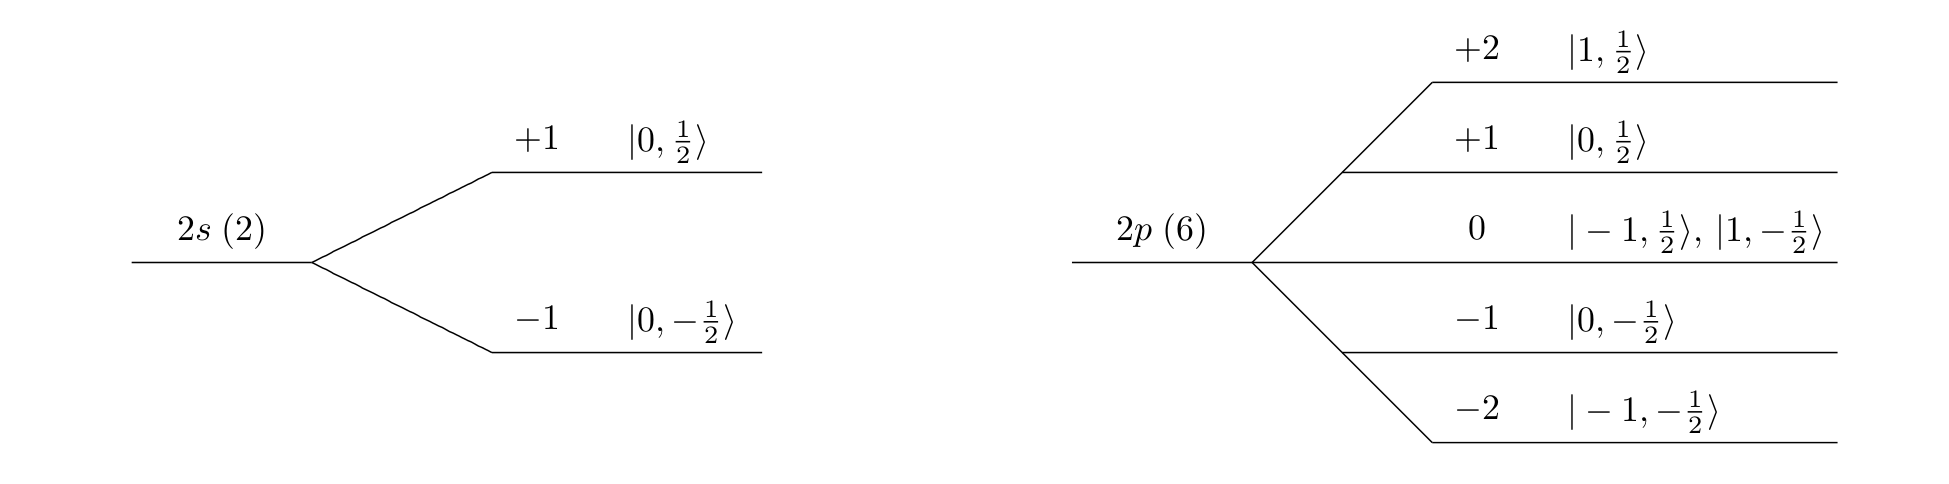
\includegraphics[height=4cm ,width=16cm]{QM/zeeman1.png}
	\caption{Zeeman effect for $n=2$ in Hydrogen atom}
\end{figure}
\\ \\
If $H_{\mathrm{FS}}$ is much smaller than $H_{\mathrm{Z}}$ and but cannot be neglected, we may treat it as a perturbation. For simplicity, we only take $H_{\mathrm{SO}}$ into account. Up to the first order, we consider the matrix element
\[\langle n l m_l m_s | f(r)\bm{L}\cdot\bm{S}| n l' m'_l m'_s\rangle.\]
Since $[H_{\mathrm{SO}},L^2] = 0$, the term above vanishes unless $l = l'$. Thus we focus on the matrix in the subspace $l = l'$. For the $2p$ orbit of hydrogen, there is a 2-fold degeneracy between $|2,1,-1,\frac{1}{2}\rangle$ and $|2,1,1,-\frac{1}{2}\rangle$.
This makes one $2 \times 2$ matrix. Let us look at the off-diagonal element,
\[\langle 2,1,-1,\frac{1}{2} | f(r)\bm{L}\cdot\bm{S}| 2,1,1,-\frac{1}{2}\rangle,\]
in which we use the identity
\[\bm{L}\cdot\bm{S} = \frac{1}{2}(L_+S_-+L_-S_+)+L_zS_z.\]
To be non-vanishing, the operator in the middle of the matrix element must connect states with $\Delta m_l = 2$, but in fact that operator permits only $\Delta_m = 0,\pm1$. Therefore the off-diagonal matrix element vanishes and the energy shift is determined by diagonal elements. For $2p$ orbit, we can get
\[\Delta E = \langle n l m_l m_s | f(r)\bm{L}\cdot\bm{S}| n l m_l m_s\rangle \propto m_lm_s.\]
As for the $2s$ levels, for them $\bm{L} = 0$ (that is, the operator $\bm{L}$ vanishes on the 2s-subspace), so $\Delta E = 0$.
\\ \\
The final case we shall examine is the weak field limit, in which $H_z \ll H_{\mathrm{FS}}$ and we will treat $H_z$ as perturbation.
\begin{note}
In the case of hydrogen, one should also consider the Lamb shift for a realistic treatment. For example, in the $n=2$ levels of hydrogen, the Lamb shift is about $10$ times smaller than the fine structure energy shifts, indicating that we really should question how the Lamb shift compares to the Zeeman term which is also (by our assumptions) much smaller than the fine structure term.
\end{note}
\noindent
The eigenvector of $H_a + H_{\mathrm{FS}}$ are $|nljm_j\rangle$ with eigenvalue $E_{nj}$. Up to the first order,the matrix elements we need have the form
\[\langle n l' j m'_j | H_z | n l j m_j\rangle.\]
Since $[H_{\mathrm{Z}},L^2] = 0$ and $[H_{\mathrm{Z}},J_z] = 0$, off-diagonal matrix element vanishes automatically.The energy shift is
\[\Delta E = \mu_{\mathrm{B}} B\langle n l j m_j | L_z + 2S_z | n l j m_j\rangle = g_{\mathrm{eff}} \mu_{\mathrm{B}} B m_j,\]
where
\[g_{\mathrm{eff}} = 1 + \frac{j(j+1)-l(l+1)+s(s+1)}{2j(j+1)}.\]

\subsection{Hyperfine structure}
The nucleus of an atom contains localized charge and current distributions, which produce electric and magnetic fields that can be decomposed into multipole fields much as in classical electrostatics or magnetostatics.
The first of the multipole moments, the electric monopole, is of course the Coulomb electrostatic field that holds the electrons in their orbits and produces the gross structure of the atom.
The higher order multipole moments produce small corrections to the atomic structure that are known generally as hyperfine effects.
\\ \\
Multipole moments for a system of charges has been discussed in the part of classical electrodynamics. In quantum mechanics, we recall that the intrinsic magnetic moment operator of an electron is defined in the space of electron spin. Thus we may infer that multipole moments of nuclei is defined in the space of nuclear spin $\bm{I}$. 
We let the quantum number of the operator $I^2$ be $i$, so that $I^2$ has eigenvalues $i(i+1)$. The nuclear Hilbert space is a  $(2i+1)$ dimensional space in which the standard basis is $|im_i\rangle$ with $-i \leq m \leq i$.\\ \\
Not all the multipole fields that occur classically are allowed in the case of a nuclei. There are two rules governing the allowed multipole moments of the nucleus.
The first is that electric multipoles of odd $k$ and magnetic mutlipoles of even $k$ are forbidden. For example, if the nucleus had an electric dipole moment, the perturbing Hamiltonian would be
\[H_1 = -e \frac{\bm{d}\cdot\bm{r}}{r^3}.\]
And just like $\bm{\mu}$,$\bm{d}$, must be proportional to the spin, say $\bm{d} = \kappa\bm{I}$, because all vector operators on a single irreducible subspace are proportional (Wigner-Eckart theorem). Thus,
\[H_1 = -\kappa e \frac{\bm{I}\cdot\bm{r}}{r^3}.\]
We find that $H_1$ violates time reversal and parity
\[T H_1 T^{\dagger} = -H_1 , \quad P H_1 P^{\dagger} = -H_1.\]
The weak interactions do violate parity, and we do know that time reversal (more precisely, CP) is violated at a very small  level in certain decay processes, so it is possible that the terms forbidden by this rule actually exist at a small level. For example, the neutron or the electron may have an electric dipole moment, but if such moments exist, they are certainly very small and can be neglected in our discussion.
\\ \\
The second rule states that a $2^k$-pole can occur only if $k \leq 2i$. For example, the proton with $i = {1}/{2}$ can possess an electric monopole moment and a magnetic dipole moment, but not an electric quadrupole moment. Lying behind this rule is the fact that the operator representing the $2^k$ -pole on the nuclear Hilbert space is, in fact, an order $k$ irreducible tensor operator. But the maximum order of an irreducible tensor operator on the nuclear Hilbert space with
spin $i$ is $k = 2i$.
\\ \\
Thus for hydrogen atom, whose nuclear spin is $i = {1}/{2}$, the only term we have to concern is magnetic moment. A point magnetic dipole of moment $\bm{\mu}$ is
\[\bm{A}(\bm{r}) = \frac{\bm{\mu}\times\bm{r}}{r^3}.\]
To avoid the singularity at origin, we modify $\bm{A}(\bm{r})$ as
\[\bm{A}(\bm{r}) = \bm{\mu}\times\bm{r} \begin{cases} \frac{1}{a^3} , \quad r < a\\ \frac{1}{r^3} , \quad r > a\end{cases} ,\]
taking into account of the finite size of nuclei. 
By taking the curl we compute the magnetic field
\[\bm{B}(\bm{r}) =  \begin{cases} \frac{2\bm{\mu}}{a^3} , \quad r < a\\ \bm{\mu}\cdot\hat{T} , \quad r > a\end{cases} ,\]
where $T_{ij} = (3x_ix_j-r^2\delta_{ij})/{r^5}$
We define
\[\Delta(r) \equiv \begin{cases} \frac{1}{a^3} , \quad r < a\\ 0 , \quad r > a\end{cases},\]
and
\[f(r) \equiv \begin{cases} 0 , \quad r < a\\ 1 , \quad r > a\end{cases}.\]
Then we can write
\[\bm{A}(\bm{r}) = \bm{\mu}\times\bm{r} \left [\Delta(r) + \frac{f(r)}{r^3}\right ] \]
and
\[\bm{B}(\bm{r}) = \bm{\mu}\cdot \left [2\Delta(r)\hat{I} + f(r)\hat{T}\right ] .\]
In the limit $a \to 0$, we have
\[\lim_{a \to 0} \Delta(r) = \frac{4\pi}{3}\delta(\bm{r}) , \quad \lim_{a \to 0} f(r) = 1.\]
The Hamiltonian of the system is
\[H = \frac{(\bm{P}+e\bm{A})^2}{2m} - \frac{e^2}{4\pi r} + H_{\mathrm{FS}} + H_{\mathrm{Lamb}} + \frac{e}{m}\bm{S}\cdot\bm{B}.\]
The expressions  for $\bm{A}$ and $\bm{B}$ are are given above and $\bm{\mu}$ in the expression are given by
\[\bm{\mu} = g_{p} \mu_{\mathrm{p}} \bm{I},\]
where $g_{\mathrm{p}}$ is g-factor of proton and $\mu_{\mathrm{p}} \equiv {e}/{2m_p}$. 
Thus, the Hamiltonian must be interpreted as an operator acting the total Hilbert space
\[\mathcal{H} = \mathcal{H}_{\mathrm{elec}} \otimes \mathcal{H}_{\mathrm{nucl}}.\]
For $\mathcal{H}_{\mathrm{elec}}$ the obvious basis is $|nljm_j\rangle$ with energies $E_{nlj}$ when there is no hyperfine terms. In hydrogen energies depend on $l$ because of the Lamb shift. The obvious basis in $\mathcal{H}_{\mathrm{nucl}}$ is $|im_i\rangle$. Thus we define the basis states in $\mathcal{H}$ as $|nljm_jm_i\rangle$ (we suppress the index $i$ since it is a constant).It is called uncoupled basis. Now we expand the Hamiltonian and neglect the term $A^2$, writing the result as $H = H_0 + H_1$ , where
\[H_0 = \frac{p^2}{2m} - \frac{e^2}{4\pi r}  + H_{\mathrm{FS}} + H_{\mathrm{Lamb}}\]
and
\[H_1 = 2\mu_{\mathrm{B}}(\bm{P}\cdot\bm{A} + \bm{S}\cdot\bm{B}).\]
Since
\[\bm{P}\cdot(\bm{I}\cdot\bm{r}) = \bm{I}\cdot(\bm{r}\cdot\bm{P}) = \bm{I}\cdot\bm{L},\]
we have
\[H_{1,\mathrm{orbi}} \equiv 2\mu_{\mathrm{B}}(\bm{P}\cdot\bm{A}) = k(\bm{I}\cdot\bm{L}) \left[\Delta(r) + \frac{f(r)}{r^3}\right ].\]
where $k \equiv g_{\mathrm{e}}g_{\mathrm{p}}\mu_{\mathrm{B}}\mu_{\mathrm{p}}$.
On the other hand, we have
\[H_{1,\mathrm{spin}} \equiv 2\mu_{\mathrm{B}} \bm{S}\cdot\bm{B} = k\left [2\Delta(r)\bm{I}\cdot\bm{S} + f(r)\bm{I}\cdot\hat{T}\cdot\bm{S}\right ] .\]
In the limit $a \to 0$, we have
\[H_{1,\mathrm{orbi}} = k(\bm{I}\cdot\bm{L}) \left[\frac{4\pi}{3}\delta(\bm{r}) + \frac{1}{r^3}\right ]\]
and
\[H_{1,\mathrm{spin}}  = k\left [\frac{8\pi}{3}\delta(\bm{r})\bm{I}\cdot\bm{S} + \bm{I}\cdot\hat{T}\cdot\bm{S}\right ] .\]
Since the coupling term (e.g. $\bm{I}\cdot\bm{S}$) are not invariant under either electronic rotations alone or under nuclear rotations alone. The uncoupled basis is not the best one for carrying out the perturbation calculation. The total angular momentum of the system are defined by
\[\bm{F} \equiv \bm{I} + \bm{J} = \bm{I} + \bm{L} + \bm{S}.\]
The new coupled basis is $|nljfm_f\rangle$. Since $[\bm{F},H] = 0$, $|nljfm_f\rangle$ is the eigenvector of $H$. The energy shift caused by $H_1$ is
\[\Delta E = \langle nljfm_f | H_1 | nljfm_f\rangle.\]
After a lengthy calculation, we can get
\[\Delta E = \frac{g_{\mathrm{e}}g_{\mathrm{p}}\mu_{\mathrm{B}}\mu_{\mathrm{p}}}{4\pi a_0^3} \frac{1}{n^3} \frac{f(f+1)-j(j+1)-i(i+1)}{j(j+1)(2l+1)} .\]
The energy levels were $E_{nlj}$ before the hyperfine interactions were turned on, but since $\Delta E$ depends on $f$, they now have the form $E_{nljf}$ . The energy eigenstates are $|nljfm_f\rangle$, and are $(2f+1)$-fold degenerate, causing the fine structure levels of hydrogen to split, giving rise to hyperfine multiplets. 
For example, the ground state $|1,0,\frac{1}{2}\rangle$ splits into two levels $f = 0$ and $f = 1$. This $f = 0$ level is the true ground state of hydrogen. It is nondegenerate. The $f=1$ level is 3-fold degenerate, and lies above the ground state by an energy of approximately $1.42 \mathrm{GHz}$ in frequency
units, or $21 \mathrm{cm}$ in wave length units.

\section{Time dependent perturbation theory}
\subsubsection{Dyson series}
Time-dependent perturbation theory applies to Hamiltonians of the form
\[H = H_0 + H_1(t),\]
where $H_0$ is solvable and $H_1$ is treated as a perturbation.In time-dependent perturbation theory, we are usually interested in time-dependent transitions between eigenstates of the unperturbed system induced by the perturbation $H_1$.
Time-dependent transitions are usually described by the transition amplitude, defined as the quantity
\[\langle f | U(t) | i \rangle,\]
where $U(t)$ is the exact time evolution operator for the Hamiltonian, and where $|i\rangle$ and $|f\rangle$ are
two eigenstates of the unperturbed Hamiltonian $H_0$. 
Let us denote the unperturbed time-evolution operator by $U_0(t)$ and the exact one by $U(t)$.
These operators satisfy the evolution equations
\[i\frac{\partial U_0(t)}{\partial t} = H_0U_0(t) , \quad i\frac{\partial U(t)}{\partial t} = HU(t).\]
Since $H_0$ is independent of time, we have $U_0 = e^{-iH_0 t}$.\\ \\
Suppose the state in Schr\"{o}dinger picture is $|\psi_S(t)\rangle$, then we define the state in interaction picture as
\[|\psi_{\mathrm{I}}(t)\rangle \equiv U^{\dagger}_0(t) |\psi_{\mathrm{S}}(t)\rangle.\]
Similarly, we define the operator in interaction picture as
\[A_{\mathrm{I}}(t) \equiv U^{\dagger}_0(t) A_{\mathrm{S}}(t) U_0(t).\]
Let us define $W(t)$ as the operator that evolves kets in the interaction picture forward from time $0$ to final time $t$, i.e.
\[ |\psi_{\mathrm{I}}(t)\rangle = W(t) |\psi_{\mathrm{I}}(0)\rangle .\]
We can verify that
\[W(t) = U^{\dagger}_0U(t).\]
And we can get the time evolution of $W(t)$
\[i\frac{\partial W}{\partial t} = H_{1\mathrm{I}}(t)W(t).\]
The formal solution is
\[W(t) = I + (-i)^n \sum_{n=1}^{\infty} \int_{0}^{t}dt_1 \int_{0}^{t_1}dt_2 \cdots \int_{0}^{t_{n-1}} dt_n H_{1\mathrm{I}}(t_1)H_{1\mathrm{I}}(t_2)\cdots H_{1\mathrm{I}}(t_n).\]
Let us assume for simplicity that $H_0$ has a discrete spectrum $H_0|n\rangle = E_n|n\rangle$. 
We assume that the system is initially in an eigenstate of the unperturbed system, what we will call the ``initial'' state $|i\rangle$ with energy $E_{\mathrm{i}}$. Then 
\[|\psi_{\mathrm{I}}(t)\rangle = W(t)|i\rangle.\]
Let us expand the exact solution of the Schr\"{o}dinger equation in the interaction picture in the unperturbed eigenstates
\[|\psi_{\mathrm{I}}(t)\rangle = \sum_n c_n(t) |n\rangle.\]
We then have
\[c_n(t) = \langle n | W(t) | i\rangle = \langle n | U^{\dagger}_0U(t) | i\rangle = e^{iE_nt} \langle n | U(t) | i\rangle .\]
Thus the transition amplitudes in the interaction picture and those in the Schr\"{o}dinger picture are related by a simple phase factor.The transition probabilities are the squares of the amplitudes and are the same in either case. The perturbation expansion of the transition amplitude $c_n(t)$ is
\[c_n(t) = \delta_{ni} + c^{(1)}_n(t) + \cdots\]
where
\[c^{(1)}_n(t) = \frac{1}{i} \int_0^t dt' \langle n | H_{1\mathrm{I}}(t')|i\rangle = \frac{1}{i} \int_0^t dt' e^{i(E_n-E_{\mathrm{i}})t'} \langle n | H_{1}(t')|i\rangle.\]

\subsubsection{Constant and harmonic perturbation}
If $H_1$ is time-independent, we have
\[c^{(1)}_n(t) = \frac{2}{i} e^{i\omega_{ni}t/2} \left( \frac{\sin\omega_{ni}t/2}{\omega_{ni}} \right) \langle n | H_1 | i \rangle.\]
Up to the first order, the transition probability is
\[P_n(t) = 4 \left( \frac{\sin^2\omega_{ni}t/2}{\omega_{ni}^2} \right) |\langle n | H_1 | i \rangle|^2 , \quad (n \neq i).\]
Another case that is important in practice is when $H_1$ has a periodic time dependence of the form
\[H_1(t) = Ke^{-i\omega_0t} + K^{\dagger}e^{i\omega_0t}.\]
We can get
\[c^{(1)}_n(t) = \frac{2}{i} \left[ e^{i(\omega_{ni}-\omega0)t/2} \left( \frac{\sin(\omega_{ni}-\omega_0)t/2}{\omega_{ni}-\omega_0} \right) \langle n | K | i \rangle  + e^{i(\omega_{ni}+\omega_0)t/2} \left( \frac{\sin(\omega_{ni}+\omega_0)t/2}{\omega_{ni}+\omega_0} \right) \langle n | K^{\dagger} | i \rangle \right]  .\]
Often, we are most interested in those final states to which most of the probability goes, which are the states for which one or the other of the two denominators is small.
For these states we have
\[E_n \approx E_{\mathrm{i}} \pm \omega_0.\]
We call these two cases absorption and stimulated emission, respectively. 
Taking the case of absorption, and looking only at final states that are near resonance, we can write the transition probability to first order of perturbation theory as
\[P_n(t) = 4 \left( \frac{\sin^2(\omega_{ni}-\omega_0)t/2}{(\omega_{ni}-\omega_0)^2} \right) |\langle n | K | i \rangle|^2.\]

\subsubsection{Transition probability}
Let us fix the final state and examine how the probability develops as a function of time in first order time-dependent perturbation theory.
Obviously $P_n(0) = 0$. At later times we see that $P_n(t)$ oscillates at frequency $\omega_{ni}$ between $0$ and a maximum proportional to ${1}/{\omega_{ni}}$.
The frequency $\omega_{ni}$ measures how far the final state is off resonance, that is, how much it fails to conserve energy. If this frequency is large, the probability oscillates rapidly between zero and a small maximum. 
But as we move the state closer to the initial state in energy, $\omega_{ni}$ gets smaller, the period of oscillations becomes longer, and the amplitude grows.
If there is a final state degenerate in energy with the initial state, then $\omega_{ni}=0$ and the time-dependent factor takes on its limiting value ${t^2}/{4}$. In this case, first order perturbation theory predicts that the probability grows without bound.
This is an indication of the fact that at sufficiently long times first order perturbation theory breaks down and we must take into account higher order terms in the perturbation expansion. But at short times it is correct that $P_n$ for a state on resonance grows as $t^2$.
\\ \\
Now let us fix the time $t$ and examine how the expression for $P_n(t)$ in first order perturbation theory depends on the energy of the final state. To do this we focus on ${\sin^2(\omega t/2)}/{\omega^2}$ as a function of $\omega$.
The curve of the function consists of oscillations under the envelope ${1}/{\omega^2}$, with zeroes at $\omega = {2n\pi}/{t}$. 
The central lobe has height ${t^2}/{4}$ and width that is proportional to ${1}/{t}$, so the area of the central lobe
is proportional to $t$.
We can derive that
\[\lim_{t \to \infty} \frac{1}{t} \frac{\sin^2\omega t/2}{\omega^2} = \frac{\pi}{2}\delta(\omega).\]
The $\delta$-function enforces energy conservation in the limit $t \to \infty$. But at finite times, transitions take place to states in a range of energies about the initial energy.
This width is of order ${1}/{t}$. This is an example of the energy-time uncertainty relation, $\Delta t \Delta E \sim 1$, indicating that a system that is isolated (not
subjected to a measurement) over a time interval $\Delta t$ has an energy that is uncertain by an amount $\Delta E \sim {1}/{\Delta t}$.
\\ \\
It is conventional to define the transition rate as the transition probability per unit time,i.e.
\[\Gamma(i \to f) = \lim_{t \to \infty}\frac{P(i \to f)}{t}.\]
Up to the first order, we have
\[\Gamma(i \to f) = 2\pi \delta(E_{\mathrm{i}} - E_{\mathrm{f}}) |V_{\mathrm{fi}}|^2,\]
where $V_{\mathrm{fi}} = \langle f | H_1 | i \rangle$.

\section{Atomic radiation}
We apply time-dependent perturbation theory to the interaction of atomic electron with the classical radiation field.
The basic Hamiltonian, with $A^2$ omitted, is
\[H = \frac{p^2}{2m} - e\phi(\bm{x}) + \frac{e}{m}\bm{A}\cdot\bm{P}.\]
Specifically, we work with a linear polarized monochromatic field of the plane wave for
\[\bm{A} = 2A_0\bm{\epsilon}\cos(\bm{k}\cdot\bm{x}-\omega t) = A_0\bm{\epsilon} [e^{i\bm{k}\cdot\bm{x}}e^{-i\omega t}  + e^{-i\bm{k}\cdot\bm{x}}e^{i\omega t} ].\]
Therefore, ${e}\bm{A}\cdot\bm{P} / m$ is a Harmonic perturbation with $K = {eA_0} e^{i\bm{k}\cdot\bm{x}} (\bm{\epsilon}\cdot\bm{P})/m$.
For example, take the case of absorption, the transition rate is
\[\Gamma_{\rm abs}(1 \to 2) = 2\pi \frac{e^2|A_0|^2}{m^2} |\langle 2 |e^{i\bm{k}\cdot\bm{x}} (\bm{\epsilon}\cdot\bm{P}) |1 \rangle|^2 \delta(E_{\mathrm{f}}-E_{\mathrm{i}}-\omega).\] 
Since the amplitude $|A_0|$ is associated with the average energy density of the EM field through
\begin{equation}
	\rho = \frac{1}{2}\overline{(\bm{E}^2 + \bm{B}^2)} = 2\omega^2|A_0|^2,
\end{equation}
the transition rate can be rewritten as
\[\Gamma_{\rm abs}(1 \to 2) = \pi \frac{e^2}{m^2\omega^2} |\langle 2 |e^{i\bm{k}\cdot\bm{x}} (\bm{\epsilon}\cdot\bm{P}) |1 \rangle|^2 \rho \delta(E_{2}-E_{1}-\omega) = \pi \frac{e^2}{m^2\omega^2} |\langle 2 |e^{i\bm{k}\cdot\bm{x}} (\bm{\epsilon}\cdot\bm{P}) |1 \rangle|^2 \rho(\omega_{\rm 21}),\]
where $\rho(\omega)$ is the average energy density of the EM field per unit angular frequency.
\\ \\
The electrical dipole approximation is based on the fact that the wavelength of radiation field is far longer than the atomic dimension, so that the series
\[e^{i\bm{k}\cdot\bm{x}} = 1+ i\bm{k}\cdot\bm{x}+\cdots\]
can be approximated by its leading term, $1$. We now have
\[\langle 2 |e^{i\bm{k}\cdot\bm{x}} (\bm{\epsilon}\cdot\bm{P}) |1 \rangle = \bm{\epsilon} \cdot \frac{m}{i} \langle 2 |  [\bm{x},H_0] |1 \rangle = im(E_2-E_{1})\langle 2 | \bm{\epsilon} \cdot \bm{x} |1 \rangle  .\]
where $H_0 = {p^2}/{2m} - e\phi(\bm{x})$.
Recall the Wigner-Eckart theorem, we have the selection rules: 
If the EM wave is linear polarized in $z$ direction, the matrix element would vanish unless $\Delta m = 0$ and $\Delta l = \pm 1$ ($\Delta l $ can not be $0$ because parity consideration). 
If the EM wave is circular polarized, we would have $\Delta m = \pm 1$. If the fine structure is taken into account, we would have $\Delta j = 0,\pm 1$ and $\Delta l = \pm 1$. If the hyperfine structure is taken into account, we would have $\Delta f = 0,\pm 1$, $\Delta j = 0,\pm 1$ and $\Delta l = \pm 1$. 
In this case, the absorption rate can be simplified to
\begin{equation}
	\Gamma_{\rm abs}(1 \to 2) = \pi |\langle 2 | \bm{\epsilon}\cdot\bm{d} | 1 \rangle |^2 \rho(\omega_{21}),
\end{equation}
where $\bm{d} \equiv e\bm{x}$ is the electrical dipole operator. 
If we assume the direction and polarization of the incident light is totally random, we have
\begin{equation}
	|\langle 2 | \bm{\epsilon}\cdot\bm{d} | 1 \rangle |^2 = \frac{1}{3}d_{21}^2,
\end{equation}
where $d_{21}^2 \equiv |\langle 2 | \bm{d} | 1 \rangle |^2$.
If we take the degeneracy of state $|2\rangle$ into account, we have
\begin{equation}
	\Gamma_{\rm abs}(1 \to 2) = B_{1 \to 2}\rho(\omega_{21}),
\end{equation}
where $B_{1 \to 2} \equiv {\pi g_2 d_{21}^2}/{3}$.
Similarly, we can also get the rate of stimulated emission,
\begin{equation}
	\Gamma_{\rm emm}(2 \to 1) = B_{2 \to 1}\rho(\omega_{21}),
\end{equation}
where $B_{2\to 1} \equiv {\pi g_1 d_{12}^2}/{3}$. 
We can see that $B_{1\to 2}$ and $B_{1\to 2}$ are exactly the Einstein coefficients of absorption and stimulated emission. And the relation $g_{2}B_{2\to 1} = g_{1}B_{1\to 2}$ is obvious. 
However, spontaneous emission can not be explained unless we quantize the EM field as well. A complete treatment of atomic radiation by quantum field theory can be found in section 4.5 of \emph{Theoretical astrophysics, Volume 1(T. Padmanabhan)}.

\section{Variational method}
\subsection{The formulation of variational method}
Let $H$ be a Hamiltonian which is assumed to have some bound states. Let the discrete (bound state) energy eigenvalues be ordered $E_0 < E_1 < \cdots$. The eigenvalues are allowed to be degenerate. There may also be a continuous spectrum above some energy, as often happens in practice.
Let $|\psi\rangle$ be any normalizable state. Then the theorem states that
\[\frac{\langle \psi | H | \psi \rangle}{\langle \psi | \psi \rangle} > E_0.\]
The state $|\psi\rangle$ is chosen to be an approximation to the ground state, based on physical intuition or other criteria, and the upper bound on $E_0$ that is obtained is often quite useful.
In practice we often choose a continuous family of trial wave functions. Let $\lambda$ be a continuous parameter, and let us write the family as $|\psi(\lambda)\rangle$. Then we define a function of $\lambda$, really an energy function,
\[F(\lambda) = \frac{\langle \psi(\lambda) | H | \psi(\lambda) \rangle}{\langle \psi(\lambda) | \psi(\lambda) \rangle}.\]
We minimize this by finding the root $\lambda_0$ of
\[\frac{\partial F}{\partial \lambda} = 0\]
so that the best estimate to the ground state wave function out of the family is $|\psi(\lambda)\rangle$ and the best estimate for the ground state energy is $F(\lambda_0)$. 
Of course we must check that the root is actually a minimum.
\\ \\
In practice the normalization denominators are often inconvenient. One possibility is simply to normalize each member of the set of trial wave functions so those denominators are not
present. 
But often it is easier to enforce normalization by using Lagrange multipliers. We introduce the function,
\[F(\lambda,\beta) = \langle \psi(\lambda) | H | \psi(\lambda) \rangle - \beta (\langle \psi(\lambda) | \psi(\lambda) \rangle - 1),\]
and then require
\[\frac{\partial F}{\partial \lambda} = 0 , \quad \frac{\partial F}{\partial \beta} = 0.\]

\subsection{Bound states and the virial theorem}
Suppose the potential scales as $V(\lambda \bm{x}) = \lambda^n V(\bm{x})$. We will assume that there is a normalised ground state with wave function $\psi_0(\bm{x})$.
The ground state energy is
\[E_0 = \int d^d\bm{x} \; -\frac{1}{2m}|\nabla\psi_0(\bm{x})|^2 + V(\bm{x})|\psi_0(\bm{x})|^2 \equiv \langle T \rangle_0 + \langle V \rangle_0.\] 
Now consider the trial wave function $\psi(\bm{x}) = \alpha^{d/2} \psi_0(\bm{x})$, where the prefactor ensures
that $\psi(\bm{x})$ continues to be normalised. 
From the scaling property of the potential, it is simple to show that
\[E(\alpha) = \alpha^2 \langle T \rangle_0 + \alpha^{-n} \langle V \rangle_0.\]
The minimum of $E(\alpha)$ is at
\[\frac{dE}{d\alpha} = 2\alpha\langle T \rangle_0 -n\alpha^{-n-1}\langle V \rangle_0 = 0.\]
But this minimum must sit at $\alpha = 1$ since, by construction, this is the true ground state. We learn that for the homogeneous potentials, we have
\[2\langle T \rangle_0 = n\langle V \rangle_0.\]
This is the virial theorem.
\begin{example}
$V \sim -1/r$. This is the Coulomb potential. The virial theorem tells us that $E_0 = \langle T \rangle_0 +  \langle V \rangle_0 = -\langle T \rangle_0 < 0$. In other words, we proved what we already know: the Coulomb potential has bound states.
\end{example}

\begin{note}
Nowhere in our argument of the virial theorem did we state that the potential must be attractive. Our conclusion above would seem to hold for repulsive potential, yet this is clearly wrong: the repulsive potential $V \sim +1/r$ has
no bound states. 
It is because we assumed at the beginning of the argument that the ground state $\psi_0$ was normalisable. For repulsive potentials this is not true: all states are asymptotically plane waves of the form $e^{ikx}$. 
The virial theorem is not valid for repulsive potentials of this kind.
\end{note}

\noindent
There is an exact and rather pretty result that holds for particles moving in one-dimension.
Consider a particle moving in a potential $V(\bm{x})$ such that $V(x) = 0$ for $|x| > L$. A bound state exists whenever $\int dx V(x) < 0$. In other words, a bound state exists whenever the potential is ``mostly attractive''. However, the converse to this statement does not hold. The proof can be found in subsection 6.1.2 of \emph{Applications of Quantum Mechanics (David Tong)}. 

\section{WKB method}
\begin{note}
In this section, we will write $\hbar$ explicitly in our equation.
\end{note}
\subsection{The semi-classical expansion}
Consider the one-dimensional time independent Schrödinger equation
\[-\frac{\hbar^2}{2m} \frac{d^2 \psi}{dx^2} + V(x)\psi = E\psi.\]
We will look for solutions of the form
\[\psi(x) = e^{iW(x)/\hbar}.\]
Plugging this ansatz into the Schr\"{o}dinger equation leaves us with the differential equation
\[i\hbar \frac{d^2W}{dx^2} - \left( \frac{dW}{dx} \right)^2 + p(x)^2 = 0,\]
where $p(x)^2 = 2m(E-V(x))$.
Here we'll look for solutions where the second derivative is merely small, meaning
\[\hbar \left| \frac{d^2W}{dx^2} \right| \ll \left| \frac{dW}{dx} \right|^2.\]
We refer to this as the semi-classical limit. Roughly speaking, it can be thought of as the $\hbar \to 0$ limit. Indeed, mathematically, it makes sense to attempt to solve Schr\"{o}dinger using a power series in $\hbar$. 
We treat $p(x)$ as the background potential which we will take to be $O(\hbar^0)$. We expand our solution as
\[W(x) = W_0(x) + \hbar W_1(x) + \cdots\]
Plugging this ansatz gives
\[\left[-W'_0(x)^2 + p(x)^2 \right] + \hbar \left[ iW''_0(x) - 2W'_0(x)W'_1(x) \right] + O(\hbar^2) = 0.\]
We have the solution
\[W_0(x) = \pm \int^x dx' p(x') , \quad W_1(x) = \frac{i}{2} \log p(x) + c.\]
Putting these together gives us the WKB approximation to the wave function
\[\psi(x) \approx \frac{A}{\sqrt{p(x)}} \exp \left( \pm \frac{i}{\hbar} \int^{x'} dx' p(x')\right).\]
To leading order, our requirement reads
\[\hbar \left| \frac{dp}{dx} \right| \ll |p(x)|^2  \Rightarrow \frac{d\lambda}{dx} \ll 2\pi,\]
where $\lambda \equiv 2\pi \hbar / p$ is the de Broglie wavelength. This is the statement that the de Broglie wavelength of the particle does not change considerably over distances comparable to its wavelength.
Alternatively, we can phrase this as a condition on the potential. We have
\[\lambda(x) \left| \frac{dV}{dx} \right| \ll \frac{|p(x)|^2}{2m},\]
which says that the change of the potential energy over a de Broglie wavelength should be much less than the kinetic energy.
\\ \\
The WKB approximation does provides a solution in regions where $E \gg V(x)$ and, correspondingly, $p(x)$ is real. This is the case in the middle of the potential, where
the wave function oscillates. 
The WKB approximation also provides a solutions when
$E \ll V(x)$ , where $p(x)$ is imaginary. This is the case to the far left and far right, where the wave function suffers either exponential decay or growth
\[\psi(x) \approx \frac{A}{2m(V(x)-E)^{1/4}} \exp \left( \pm \frac{1}{\hbar} \int^x dx' \sqrt{2m(V(x') - E)}\right) .\]
The choice of $\pm$ is typically fixed by normalisability requirements.
In the region near $E = V(x)$, the WKB approximation is never valid. 
The point $x_0$ where $p(x_0) = 0$ is the classical turning point.
The key idea that makes the WKB approximation work is matching. This means that we use the WKB approximation where it is valid. But in the neighbourhood of any turning point we will instead find a different solution. This will then be matched onto our WKB solution.
In the vicinity of $x_0$, we expand the potential energy, keeping only the linear term
\[V(x) \approx E + C(x-x_0) + \cdots\]
The Schr\"{o}dinger equation is then
\[-\frac{\hbar^2}{2m} \frac{d^2\psi}{dx^2} + Cx\psi = Cx_0 \psi.\]

\subsection{A linear potential and the Airy function}
To solve the equation above, we define the dimensionless position
\[u \equiv (\frac{2mC}{\hbar^2})^{\frac{1}{3}} (x - x_0) \approx  (\frac{2m}{\hbar^2 C^2})^{\frac{1}{3}} (V - E).\]
Then the Schr\"{o}dinger equation becomes
\[\frac{d^2\psi}{du^2} - u\psi = 0.\]
This is known as the \href{http://mathworld.wolfram.com/AiryDifferentialEquation.html}{Airy equation}. The solution is the \href{http://mathworld.wolfram.com/AiryFunctions.html} {Airy function}, $\psi(u) = \mathrm{Ai}(u)$,
which is defined by integral
\[\mathrm{Ai}(u) \equiv  \frac{1}{\pi} \int_0^{\infty} dt \cos\left( \frac{t^3}{\pi} + ut \right) .\]
It can be shown that the asymptotic behaviour is given by
\[\mathrm{Ai}(u) \sim \frac{1}{2} \left( \frac{1}{\pi \sqrt{u}} \right)^{1/2} \exp\left( -\frac{2}{3} u^{3/2} \right) , \quad u \gg 0,\]
and
\[\mathrm{Ai}(u) \sim \left( \frac{1}{\pi \sqrt{-u}} \right)^{1/2} \cos\left( \frac{2}{3} u\sqrt{-u} + \frac{\pi}{4}\right) , \quad u \ll 0.\]
\\
The main purpose in introducing the Airy function is to put it to work in the WKB approximation. The asymptotic behaviour is exactly what we need to match onto the WKB solution. First consider $u \ll 0$. Here $E > V (x)$ and we have the oscillatory solution. In this region, we have
\[\mathrm{Ai}(x) \sim \left( \frac{(2mC\hbar)^{1/3}}{\pi \sqrt{2m(E-V(x))}} \right)^{1/2} \cos \left( \frac{1}{\hbar} \int_{x_0}^x dx' \mathop{\rm sgn}(C) \sqrt{2m(E-V(x'))} + \frac{\pi}{4} \right) .\]
This takes the same oscillatory form as the WKB solution. The two solutions can be patched together simply by picking an appropriate normalisation factor and phase for the WKB solution.
Similarly, in the region $u \gg 0$, the exponentially decaying form of the Airy function can be written as
\[\mathrm{Ai}(x) \sim \frac{1}{2} \left( \frac{(2mC\hbar)^{1/3}}{\pi \sqrt{2m(V-E(x))}} \right)^{1/2} \exp \left( -\frac{1}{\hbar} \int_{x_0}^x dx' \mathop{\rm sgn}(C) \sqrt{2m(V(x') - E)} \right) .\]
This too has the same form as the exponentially decaying WKB solution. This, then, is how we piece together solutions. In regions where $E > V(x)$, the WKB approximation gives oscillating solutions. 
In regimes where $E < V(x)$, it gives exponentially decaying solutions. 
The Airy function interpolates between these two regimes.

\subsection{Bound state spectrum}
\begin{figure}[!h]
	\centering
	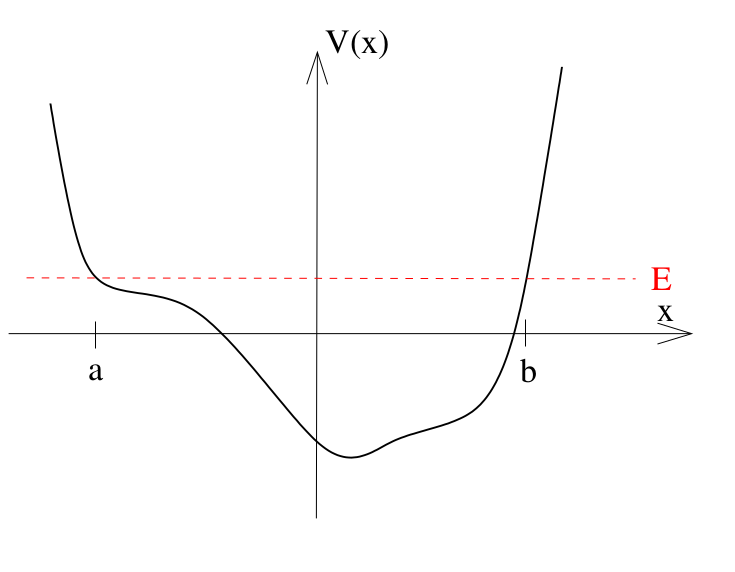
\includegraphics[scale = 0.15]{QM/wkb.png}
	\caption{One dimension potential}
\end{figure}
\noindent
We first split the potential into three regions where the WKB approximation can be trusted:
\begin{itemize}
\item Region 1: $x \ll a$.
\item Region 2: $a \ll x \ll b$.
\item Region 3: $b \ll x$.
\end{itemize}
We'll start in the left-most Region 1. Here the WKB
approximation tells us that the solution dies exponentially as
\[\psi_1(x) \approx \frac{A}{2m(V(x) - E)^{1/4}} \exp \left( -\frac{1}{\hbar} \int_{x}^a dx' \sqrt{2m(V(x')-E)} \right).\]
As we approach $x = a$, the potential takes the linear form and this coincides with the asymptotic form of the Airy function. We then follow this Airy function through to Region 2 where we have
\[\psi_2(x) \approx \frac{2A}{2m(E - V(x))^{1/4}} \cos \left( \frac{1}{\hbar} \int_{a}^x dx' \sqrt{2m(V(x')-E)} - \frac{\pi}{4} \right).\]
The Airy function takes this form close to $x = a$ where $V(x)$ is linear. But we can extend this solution throughout Region 2 where it coincides with the WKB approximation.
We now repeat this procedure to match Regions 2 an 3. When $x \gg b$, the WKB approximation tells us that the wave function is
\[\psi_1(x) \approx \frac{A'}{2m(V(x) - E)^{1/4}} \exp \left( -\frac{1}{\hbar} \int_{b}^x dx' \sqrt{2m(V(x')-E)} \right).\]
Matching to the Airy function across the turning point $x = b$, we have
\[\psi_2(x) \approx \frac{2A'}{2m(E - V(x))^{1/4}} \cos \left( \frac{1}{\hbar} \int_{b}^x dx' \sqrt{2m(V(x')-E)} + \frac{\pi}{4} \right).\]
We're left with two expressions for the wave function in Region 2.
Clearly these must agree. Equating the two tells us that $|A| = |A'|$, but they may differ by a sign, since this can be compensated by the cos function. Insisting that the two cos functions agree, up to sign, gives us the condition
\[\int_a^b dx' \sqrt{2m(E-V(x'))} = \left( n + \frac{1}{2} \right) \hbar \pi.\]
The WKB approximation underlies an important piece of history from the pre-Schr\"{o}dinger era of quantum mechanics. 
We can rewrite the quantisation condition as
\[\oint dx \; p(x) = \left( n + \frac{1}{2} \right) h , \quad h \equiv 2\pi \hbar ,\]
where $\oint$ means that we take a closed path in phase space which, in this one-dimensional example, is from $x_{\mathrm{min}}$ to $x_{\mathrm{max}}$ and back again.
In the old days of quantum mechanics, Bohr and Sommerfeld introduced an ad-hoc method of quantisation. They suggested that one should impose the condition
\[\oint dx \; p(x) = n h \]
with $n$ an integer. They didn't include the factor of $1/2$. They made this guess because it turns out to correctly describe the spectrum of the hydrogen atom.  The WKB approximation provides an a-posteriori justification of the Bohr-Sommerfeld quantisation rule.
More generally, ``Bohr-Sommerfeld quantisation'' means packaging up a 2$d$-dimensional phase space of the system into small parcels of volume $h^d$ and assigning a quantum state to each. It is, at best, a crude approximation to the correct quantisation treatment.

\section{Slow changing Hamiltonians}
\subsection{The adiabatic approximation}
Consider a Hamiltonian $H(\lambda)$ which depends on some number of parameters $\lambda_i$. 
For simplicity, we will assume that $H$ has a discrete spectrum. We write these states as
\[H|n(\lambda)\rangle = E_n(\lambda) |n(\lambda)\rangle.\]
Let's place ourselves in one of these energy eigenstates. Now vary the parameters $\lambda_i$.
The adiabatic theorem states that if $\lambda^i$ are changed suitably slowly, then the system will cling to the energy eigenstate $|n(\lambda(t))\rangle$ that we started off in.
To see this, we want to solve the time-dependent Schr\"{o}dinger equation
\[i\frac{\partial |\psi(t)\rangle}{\partial t} = H |\psi(t)\rangle.\]
We expand the solution in a basis of instantaneous energy eigenstates
\[|\psi(t)\rangle = \sum_m a_m(t) e^{i\xi_m(t)} |m(\lambda(t))\rangle.\]
Here $a_m(t)$ are coefficients that we wish to determine, while $\xi_m(t)$ is the usual energy-
dependent phase factor
\[\xi_m(t) = - \int_0^t dt' E_m(t').\]
To proceed, we substitute our ansatz into the Schr\"{o}dinger equation to find
\[\sum_m \left[\dot{a}_m e^{i\xi_m}|m(\lambda)\rangle + a_m e^{i\xi_m} \frac{\partial }{\partial \lambda^i} |m(\lambda)\rangle\dot{\lambda}^i \right] = 0.\]
Taking the inner product with $\langle n(\lambda)|$ gives
\[\dot{a}_n = ia_n\mathcal{A}_i(\lambda) \dot{\lambda}^i - \sum_{m \neq n} a_m e^{i(\xi_m - \xi_n)} \langle n(\lambda) | \frac{\partial}{\partial \lambda^i} | m(\lambda)\rangle\dot{\lambda}^i,\]
where $\mathcal{A}_i(\lambda) \equiv i\langle n(\lambda) | \frac{\partial}{\partial \lambda^i} | n(\lambda)\rangle$.
This is called the Berry connection.
\\ \\
First, we need to deal with the second term in equation above. We will argue that this is small. 
To see this, we return to our original definition of $|m(\lambda)\rangle$ and differentiate with respect to $\lambda$,
\[\frac{\partial H}{\partial \lambda^i} |m\rangle + H \frac{\partial }{\partial \lambda^i} |m\rangle = \frac{\partial E_m}{\partial \lambda} |m\rangle + E_m \frac{\partial}{\partial \lambda^i} |m\rangle .\]
Now take the inner product with $\langle n |$ where $n \neq m$ to find
\[ \langle n | \frac{\partial}{\partial \lambda^i} | m\rangle \dot{\lambda}^i = \langle n | \frac{\partial H}{\partial \lambda^i} | m\rangle \frac{\dot{\lambda}^i}{E_m - E_n} .\]
The adiabatic theorem holds when the change of parameters $\dot{\lambda}^i$ is much smaller than the splitting of energy levels $E_m -E_n$. 
In this limit, we can ignore this term. We're then left with
\[\dot{a}_n = ia_n\mathcal{A}_i \dot{\lambda}^i.\]
This is easily solved to give
\[a_n = C_n \exp \left(i \int_{\lambda(0)}^{\lambda(t)}  \mathcal{A}_i(\lambda) d\lambda^i \right).\]
This is the adiabatic theorem. If we start at time $t = 0$ with $a_m = \delta_{mn}$, so the system is in a definite energy eigenstate $|n\rangle$, then the system remains in the state $|n(\lambda)\rangle$ as we vary $\lambda$. 
This is true as long as $\dot{\lambda}^i \ll \Delta E$.
In particular, this means that when we vary the parameters $\lambda$, we should be careful to avoid level crossing, where another state becomes degenerate with the $|n(\lambda)\rangle$ that we're sitting in. 
In this case, we will have $E_m = E_n$ for some $\m\rangle$ and all bets are off: when the states separate again, there is no simple way to tell which linear combinations of the state we now sit in.

\subsection{Berry phase}
As we vary the parameters $\lambda$, the phase of the state $|n(\lambda)\rangle$ changes but there are two contributions, rather than one. 
The first is the usual $e^{-iEt}$ phase that we expect for an energy eigenstate. But there is also a second contribution to the phase due to Berry connection.
Suppose that we vary the parameters $\lambda$ but, finally we put them back to their starting values. 
This means that we trace out a closed path in the space of parameters. The second contribution can now be written as
\[e^{i\gamma} \equiv \exp \left( i\oint_C d\lambda^i \mathcal{A}_i(\lambda) \right).\]
In contrast to the energy-dependent phase, this does not depend on the time taken to make the journey in parameter space. Instead, it depends only on the path path we take through parameter space. It is known as the Berry phase.
\\ \\
Like gauge potential in electromagnetic field theory, there is also a redundancy in the information contained in the Berry connection $\mathcal{A}_i(\lambda)$.
This follows from the arbitrary choice we made in fixing the phase of the reference states $|n(\lambda)\rangle$. We could pick a different phase for every choice of parameters $\lambda$,
\[|n'(\lambda)\rangle = e^{i\omega(\lambda)} |n(\lambda)\rangle\]
for any function $\omega(\lambda)$. 
If we compute the Berry connection arising from this new choice, we have
\[\mathcal{A}'_i = \mathcal{A}_i - \frac{\partial \omega}{\partial \lambda^i} .\]
This takes the same form as the gauge transformation.
\\ \\
Following the analogy with electromagnetism, we might expect that the physical information in the Berry connection can be found in the gauge invariant field strength which, mathematically, is known as the curvature of the connection,
\[\mathcal{F}_{ij}(\lambda) = \frac{\partial \mathcal{A}_i}{\partial \lambda^j} -  \frac{\partial \mathcal{A}_j}{\partial \lambda^i}.\]
It's certainly true that $\mathcal{F}$ contains some physical information about our quantum system, but it's not the only gauge invariant quantity of interest. In the present context, the most natural thing to compute is the Berry phase. Importantly, this too is independent of the arbitrariness arising from the gauge transformation. 
This is because $\oint \partial_i \omega d\lambda^i = 0$. Indeed, we've already seen this same expression in the context of electromagnetism: it is the Aharonov-Bohm phase.
In fact, it's possible to write the Berry phase in terms of the field strength using the higher-dimensional version of Stokes' theorem
\[e^{i\gamma} = \exp \left( i\oint_C d\lambda^i \mathcal{A}_i(\lambda) \right) = \exp \left( i\int_S dS^{ij} \mathcal{F}_{ij} \right),\]
where $S$ is a two-dimensional surface in the parameter space bounded by the path $C$.
A standard example of the Berry phase on the spin in a magnetic field can be found in section 6.3.5 of 
\emph{Applications of Quantum Mechanics (David Tong)}. 

\subsection{The Born-Oppenheimer approximation}
The Born-Oppenhemier approximation is an approach to solving quantum mechanical problems in which there is a hierarchy of scales. 
The standard example is the a bunch of nuclei, each with position $\bm{R}_{\alpha}$ mass $M_{\alpha}$ and charge $Z_{\alpha}$, interacting with a bunch of electrons, each with position $\bm{r}_i$ , mass $m$ and charge $-e$. 
The Hamiltonian is
\[H = \sum_{\alpha} \frac{\nabla^2_{\alpha}}{2M_{\alpha}} + \sum_{i} \frac{\nabla^2_{i}}{2m} + \frac{e^2}{4\pi} \left(\sum_{ij} \frac{1}{|\bm{r}_i - \bm{r}_j|} + \sum_{\alpha \beta} \frac{Z_{\alpha} Z_{\beta}}{|\bm{R}_{\alpha} - \bm{R}_{\beta}|} - \sum_{i\alpha} \frac{Z_{\alpha}}{|\bm{r}_i - \bm{R}_{\alpha}|} \right).\]
The hierarchy of scales in the Hamiltonian above arises because of the mass difference between the nuclei and the electrons. The nuclei are cumbersome and slow, while the
electrons are nimble and quick. 
Relatedly, the nuclei wave functions are much more
localised than the electron wave functions. This motivates us to first fix the positions of the nuclei and look at the electron Hamiltonian, and only later solve for the nuclei dynamics. This is the essence of the Born-Oppenheimer approximation.
To this end, we write
\[H = H_{\rm nucl} + H_{\rm el},\]
where
\[H_{\rm nucl} \equiv \sum_{\alpha} \frac{\nabla^2_{\alpha}}{2M_{\alpha}} + \frac{e^2}{4\pi}  \sum_{\alpha \beta} \frac{Z_{\alpha} Z_{\beta}}{|\bm{R}_{\alpha} - \bm{R}_{\beta}|},\]
and
\[H_{\rm el} \equiv  \sum_{i} \frac{\nabla^2_{i}}{2m} + \frac{e^2}{4\pi} \left(\sum_{ij} \frac{1}{|\bm{r}_i - \bm{r}_j|}  - \sum_{i\alpha} \frac{Z_{\alpha}}{|\bm{r}_i - \bm{R}_{\alpha}|} \right).\]
We then solve for the eigenstates of $H_{\rm el}$ , where the nuclei positions $\bm{R}$ are viewed as parameters which, as in the adiabatic approximation, will subsequently vary slowly.
For fixed $\bm{R}$, the instantaneous electron wave functions are
\[H_{\rm el} \phi_n(\bm{r};\bm{R}) = \epsilon_n(\bm{R}) \phi_n(\bm{r};\bm{R}).\]
In what follows, we will assume that the energy levels are non-degenerate. We then make the ansatz for the wave function of the full system
\[\Psi(\bm{r};\bm{R}) = \sum_n \Phi(\bm{R})\phi_n(\bm{r};\bm{R}).\]
We'd like to write down an effective Hamiltonian which governs the nuclei wave functions $\Phi(\bm{R})$. 
This is straightforward. The wave function $\Psi$ obeys
\[(H_{\rm nucl} + H_{\rm el}) \Psi = E\Psi.\]
Switching to bra-ket notation for the electron eigenstates, we can write this as
\[\sum_n \langle \phi_m | H_{\rm nucl} \Phi_n | \phi_n \rangle + \epsilon_m(\bm{R}) \Phi_m = E\Phi_m.\]
Now $H_{\rm nucl}$ contains the kinetic term $\nabla^2_{\bm{R}}$, and this acts both on the nuclei wave function, but also on the electron wave function where the nuclei positions sit as parameters. We have
\[\langle \phi_m | \nabla^2_{\bm{R}} \Phi_n | \phi_n \rangle = \sum_k \left(\delta_{mk} \nabla_{\bm{R}} + \langle \phi_m | \nabla_{\bm{R}} | \phi_k \rangle  \right) \left(\delta_{kn} \nabla_{\bm{R}} + \langle \phi_k | \nabla_{\bm{R}} | \phi_n \rangle  \right) \Phi_n.\]
As in previous subsection, we can show that
\[\langle \phi_m | \nabla_{\bm{R}} | \phi_k \rangle = \frac{\langle \phi_m | \nabla_{\bm{R}} H_{\rm el} | \phi_k\rangle}{\epsilon_k - \epsilon_m}.\]
In the spirit of the adiabatic approximation, these can be neglected as long as the motion of the nuclei is smaller than the splitting of the electron energy levels.
In this limit, we get a simple effective Hamiltonian for the nuclei. The Hamiltonian depends on the state $|\phi_n\rangle$ that the electrons sit in, and is given by
\[H_n^{\rm eff} = \sum_{\alpha} \frac{1}{2M_{\alpha}} (\nabla_{\alpha} - i\mathcal{A}_{n,\alpha})^2 + \frac{e^2}{4\pi}\sum_{\alpha \beta} \frac{Z_{\alpha} Z_{\beta}}{|\bm{R}_{\alpha} - \bm{R}_{\beta}|} + \epsilon_n(\bm{R}) .\]
We see that the electron energy level $\epsilon_n(\bm{R})$ acts as an effective potential for the nuclei. The Berry connection
\[\mathcal{A}_{n,\alpha} = i \langle \phi_n | \nabla_{\bm{R}_{\alpha}} | \phi_n \rangle\]
acts as an effective magnetic field in which the nuclei
moves.
\\ \\
The idea of the Born-Oppenheimer approximation is that we can first solve for the fast-moving degrees of freedom, to find an effective action for the slow-moving degrees
of freedom. We sometimes say that we have ``integrated out'' the electron degrees of freedom, language which really comes from the path integral formulation of quantum mechanics. 
This is a very powerful idea, and one which becomes increasingly important as we progress in theoretical physics. Indeed, this simple idea underpins the Wilsonian
renormalization group which we will meet in later courses.

\chapter{Many Body Problem}
\section{Identical particles}
If two particles are identical, their exchange must not change physical quantities, so we have
\[|\cdots\psi_j\cdots\psi_i\cdots\rangle = E_{ij}|\cdots\psi_i\cdots\psi_j\cdots\rangle = e^{i\theta} |\cdots\psi_i\cdots\psi_j\cdots\rangle,\]
where $E_{ij}$ is the operator to exchange particle $i$ and $j$ and $\psi_i$ is the quantum number to describe the state of particle $i$.
In coordinate representation, it can be expressed as
\[\Psi(\cdots\bm{x}_j\cdots\bm{x}_i\cdots) = e^{i\theta} \Psi(\cdots\bm{x}_i\cdots\bm{x}_j\cdots).\]
In three dimension space, the value of $e^{i\theta}$ can only be $\pm 1$. If the spin of the particle is integer, then the phase factor must be $1$ and the particle is called boson. If the spin of the particle is half-integer, then the phase factor must be $-1$ and the particle is called fermion. This is called spin-statistics theorem and can only be proved by relativistic quantum field theory. Here, we will take it for granted.
\begin{note}
In two dimension space, the phase $e^{i\theta}$ can be anything, and the particles that obey quantum statistics of this sort are called anyons. There is a brief introduction in chapter 12.1 and
12.2 of the book Quantum Field Theory and the Standard Model (Matthew D. Schwartz).
\end{note}
\noindent
Thus not all vectors in the space $\mathcal{H}_1\otimes\cdots\otimes\mathcal{H}_n$ are physical state. The physical states must be the eigenvectors of all $E_{ij}$ with eigenvalue $1$ ($-1$) for bosons (fermions). The space composed of physical states is the so-called Fock space. For example, suppose there are three particles with different state $a,b,c$. $|abc\rangle$ is not a physical state. The physical state for bosons is
\[\frac{1}{\sqrt{3!}} \left( |abc\rangle + |acb\rangle + |bca\rangle + |bac\rangle + |cab\rangle + |cba\rangle\right).\]
The physical state for fermions is
\[\frac{1}{\sqrt{3!}} \left( |abc\rangle - |acb\rangle + |bca\rangle - |bac\rangle + |cab\rangle - |cba\rangle\right).\]
In general, for $N$ particles filling $N$ distinct states, there are $N!$ states to start with, but there is only one totally symmetric state and one totally anti-symmetric state, and the rest of $N!-2$ states are thrown out. Therefore quantum statistics reduces the size of the Hilbert space quite dramatically.
Further more, not all Hermitian operators are physical observables. A nonphysical operator is one that takes a state in the physical subspace of the Hilbert space (one that satisfies the right symmetry under exchange), and maps it into a nonphysical state (one that does not have the right symmetry).
An example is the operator $\bm{X}_1$. We might call this the operator corresponding to the measurement of the position of
particle 1. 
The problem with this operator from a physical standpoint is that you cannot measure the position of particle 1. You can select a region of space, and ask whether there is a particle in that region. But if you find one, you cannot say whether it is particle 1 or particle 2, since they are identical. 
If $O$ is a physical observables, we must have
\[[E_{ij},O] = 0\]
for all $ij$.
\begin{figure}[!h]
	\centering
	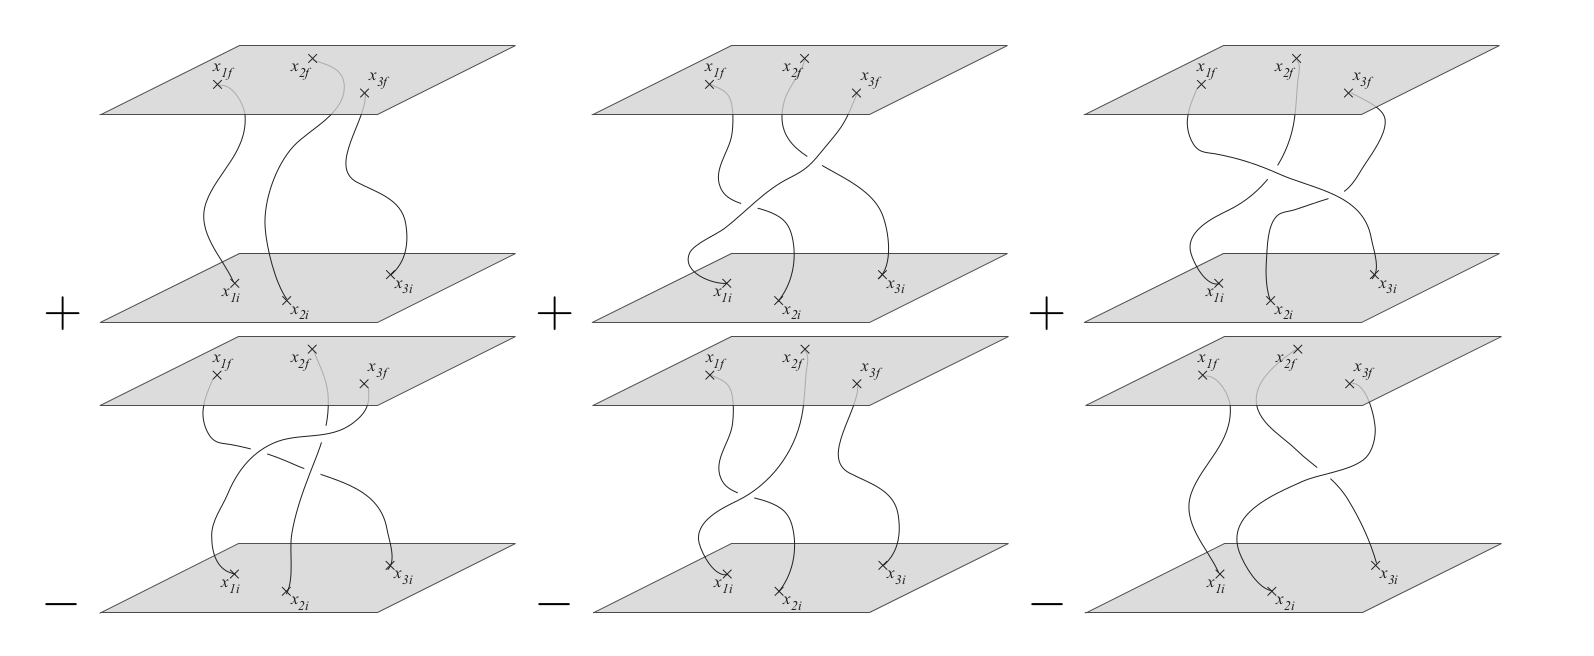
\includegraphics[height=4cm ,width=9.7cm]{QM/pathint.png}
	\caption{The path integral for three identical fermions}
\end{figure}\\
In path integral formulation of quantum mechanics, we work out the transition amplitudes
\[\langle \bm{x}_{\mathrm{f}},t_{\mathrm{f}} | \bm{x}_{\mathrm{i}},t_{\mathrm{i}}\rangle = \int \mathcal{D}\bm{x}(t) e^{i\int_{t_{\mathrm{i}}}^{t_{\mathrm{f}}} dt L(t)}.\]
The generalization to the N -particle case is
\[\langle \bm{x}_{1\mathrm{f}}\cdots\bm{x}_{N\mathrm{f}},t_{\mathrm{f}} | \bm{x}_{1\mathrm{i}}\cdots\bm{x}_{N\mathrm{i}},t_{\mathrm{i}}\rangle = \int \mathcal{D}\bm{x}_1(t)\cdots\bm{x}_N(t) e^{i\int_{t_{\mathrm{i}}}^{t_{\mathrm{f}}} dt L(t)}.\]
Here, the particle 1 at the initial position $\bm{x}_{1\mathrm{i}}$ moves to the final position $\bm{x}_{1\mathrm{f}}$, the particle 2 at the initial position $\bm{x}_{2\mathrm{i}}$ to $\bm{x}_{2\mathrm{f}}$ , etc, and you sum over all possible paths.
When the particles are identical, however, we need to introduce proper (anti-)symmetry of the state. For fermions (The case for bosons can be obtained easily by dropping all minus signs), we introduce the anti-symmetrized position bra
\[\langle [\bm{x}_1\cdots\bm{x}_N]| = \frac{1}{\sqrt{N!}} \sum_{\sigma} (-1)^{\sigma} \langle \bm{x}_{\sigma(1)}\cdots\bm{x}_{\sigma(N)}|.\]
We now consider path integral representation of the transition amplitudes
\[\langle [\bm{x}_{1\mathrm{f}}\cdots\bm{x}_{N\mathrm{f}}],t_{\mathrm{f}} | [\bm{x}_{1\mathrm{i}}\cdots\bm{x}_{N\mathrm{i}}],t_{\mathrm{i}}\rangle.\]
On the other hand, the Lagrangian for identical particles must be invariant under the exchange of particles, we can prove that
\[\langle [\bm{x}_{1\mathrm{f}}\cdots\bm{x}_{N\mathrm{f}}],t_{\mathrm{f}} | [\bm{x}_{1\mathrm{i}}\cdots\bm{x}_{N\mathrm{i}}],t_{\mathrm{i}}\rangle = \sum_{\sigma} (-1)^{\sigma}  \langle \bm{x}_{\sigma(1)\mathrm{f}}\cdots\bm{x}_{\sigma(N)\mathrm{f}},t_{\mathrm{f}} | \bm{x}_{1\mathrm{i}}\cdots\bm{x}_{N\mathrm{i}},t_{\mathrm{i}}\rangle.\]
In other words, the path integral sums over all possible paths allowing the positions at the final time slice are interchanged in all possible ways starting from the positions at the initial time slice.

\section{Non-relativistic quantum field theory}
\subsection{Motivation and formulation of quantum field theory}
There are some limitations of multi-body Schr\"{o}dinger wave function. Firstly, when the number of particles is large, multi-body Schr\"{o}dinger wave function would be cumbersome. Secondly, it is incapable of describing processes where the number of particles changes.
The aim of the quantum field theory is to come up with a formalism which is completely equivalent to multi-body Schr\"{o}dinger equations but just better:
it allows you to consider a variable number of particles all within the same framework and can even describe the change in the number of particles. 
It also gives totally symmetric or anti-symmetric multi-body wave function automatically. 
It also allows a systematic way of organizing perturbation theory in terms of Feynman diagrams.
It is particularly suited to multi-body problems.
In quantum mechanics, you start with classical particle Hamiltonian mechanics, with no concept of wave or interference. After quantizing it, we introduce Schr\"{o}dinger wave function and there emerges concepts of wave and its interference. 
In quantum field theory, you start with classical wave equation, with no concept of particle. After quantizing it, we find particle interpretation of excitations in the system.
\\ \\
Let us consider a classical field equation
\[\left (i\frac{\partial }{\partial t} + \frac{\nabla^2}{2m}\right ) \psi(\bm{x},t) = 0.\]
A solution to this field equation is that of a plane wave
\[\psi(\bm{x},t) = e^{i\bm{k}\cdot\bm{x} - i\omega t},\]
where $\omega = {k^2}/{2m}$. This classical field equation can be derived from the action
\[S = \int dt d\bm{x} \mathcal{L} , \quad \mathcal{L} = \psi^{*}\left (i\frac{\partial }{\partial t} + \frac{\nabla^2}{2m}\right ) \psi.\]
We can even add a non-linear term in the action, for instance
\[\mathcal{L} = \psi^{*}\left (i\frac{\partial }{\partial t} + \frac{\nabla^2}{2m}\right )\psi - \frac{1}{2}\lambda \psi^{*2}\psi^2.\]
Variation method gives a non-linear field equation
\[\left (i\frac{\partial }{\partial t} + \frac{\nabla^2}{2m} -\lambda \psi^*\psi\right) \psi(\bm{x},t) = 0.\]\\
Now we quantize the Schr\"{o}dinger field by canonical quantization method. A more formal discussion on the motivation and validity of canonical quantization will be discussed in relativistic quantum field theory.
The canonically conjugate momenta is
\[\pi(\bm{x}) = \frac{\partial \mathcal{L}}{\partial \dot{\psi}(\bm{x})} = i\psi^{\dagger}(\bm{x}).\] 
We now introduce canonical commutation relation
\[[\psi(\bm{x}),\pi(\bm{y})] = i\delta(\bm{x}-\bm{y}).\]
Thus
\[[\psi(\bm{x}),\psi^{\dagger}(\bm{y})] = \delta(\bm{x}-\bm{y}).\]
We now regard $\psi(\bm{x})$ as annihilation operator and $\psi(\bm{x})$ creation operator of a particle at position $\bm{x}$.
The Hamiltonian of the system is
\[H = \int d\bm{x} \left( -\psi^{\dagger}\frac{\nabla^2}{2m}\psi + \frac{1}{2}\lambda\psi^{\dagger 2}\psi^2 \right).\]
We have
\[[H,\psi^{\dagger}] = -\frac{\nabla^2}{2m}\psi^{\dagger} + \lambda \psi^{\dagger 2}\psi.\]

\subsection{Particles in quantum field theory}
We define the ``vacuum'' $|0\rangle$ which is annihilated by the annihilation operator
\[\psi(\bm{x})|0\rangle = 0\]
and construct the Fock space by
\[|\bm{x}_1\cdots\bm{x}_N\rangle = \frac{1}{\sqrt{N!}}\psi^{\dagger}(\bm{x}_1)\cdots\psi^{\dagger}(\bm{x}_N)|0\rangle .\]
The state $|\bm{x}_1\cdots\bm{x}_N\rangle$ is an $n$-particle state of identical bosons in the position eigenstate
at $\bm{x}_1\cdots\bm{x}_N$. We will verify this interpretation below explicitly.
\\ \\
Let us look at the one-particle state
\[|\bm{x}\rangle = \psi^{\dagger}(\bm{x})|0\rangle.\]
We can derive that
\[\langle \bm{y}| \bm{x}\rangle = \delta(\bm{x}-\bm{y}).\]
Therefore, this state is normalized in the same way as the one-particle position eigenstate in quantum mechanics.
We define a general one-particle state in the quantum field theory as
\[|\Psi(t)\rangle \equiv \int d\bm{x} \Psi(\bm{x},t)\psi^{\dagger}(\bm{x})|0\rangle.\]
$\psi(\bm{x})$ corresponds to the Schr\"{o}dinger wave function in the particle quantum mechanics. The Schr\"{o}dinger equation in quantum field theory is
\[i\frac{\partial |\Psi(t)\rangle}{\partial t} = H|\Psi(t)\rangle.\]
Since we can derive that
\begin{eqnarray}
H|\Psi(t)\rangle &=& \int d\bm{x} \Psi(\bm{x},t) H\psi^{\dagger}(\bm{x})|0\rangle \nonumber \\
&=& \int d\bm{x} \Psi(\bm{x},t) [H,\psi^{\dagger}](\bm{x})|0\rangle \nonumber \\
&=& \int d\bm{x} \left( -\frac{\nabla^2}{2m}\Psi(\bm{x},t) \right)|\bm{x}\rangle, \nonumber
\end{eqnarray}
we have
\[i\frac{\partial \Psi(\bm{x},t)}{\partial t} = -\frac{\nabla^2\Psi(\bm{x},t)}{2m}.\]
This is exactly the Schr\"{o}dinger equation in coordinate representation of quantum mechanics for one isolate particle.\\ \\
Let us next study the two-particle state
\[|\bm{x}_1\bm{x}_2\rangle = \frac{1}{\sqrt{2}} \psi^{\dagger}(\bm{x}_1)\psi^{\dagger}(\bm{x}_2)|0\rangle.\]
We can derive that
\[\langle \bm{x}_1\bm{x}_2 |\bm{y}_1\bm{y}_2\rangle = \frac{1}{2} \left( \delta(\bm{x}_1-\bm{y}_1)\delta(\bm{x}_2-\bm{y}_2) + \delta(\bm{x}_1-\bm{y}_2)\delta(\bm{x}_2-\bm{y}_1)\right).\]
This normalization suggests that we are dealing with a two-particle state of identical particles, because the norm is non-vanishing when $\bm{x}_1 = \bm{y}_1$ and $\bm{x}_2 = \bm{y}_2$, but also when $\bm{x}_1 = \bm{y}_2$ and $\bm{x}_2 = \bm{y}_1$, i.e., two particles interchanged. A general two-particle state is given by
\[|\Psi(t)\rangle \equiv \int d\bm{x}_1 d\bm{x}_2 \Psi(\bm{x}_1,\bm{x}_2,t)\psi^{\dagger}(\bm{x}_1)\psi^{\dagger}(\bm{x}_2)|0\rangle.\]
Because $[\psi^{\dagger}(\bm{x}_1),\psi^{\dagger}(\bm{x}_2)] = 0$, the integration over $\bm{x}_1$ and $\bm{x}_2$ is symmetric
under the interchange of $\bm{x}_1$ and $\bm{x}_2$, and hence 
$\Psi(\bm{x}_1,\bm{x}_2,t) =\Psi(\bm{x}_2,\bm{x}_1,t)$. 
The symmetry under the exchange suggests that we are dealing with identical bosons.
Since
\begin{eqnarray}
H|\Psi(t)\rangle &=& \frac{1}{\sqrt{2}} \int d\bm{x}_1 d\bm{x}_2 \Psi(\bm{x}_1,\bm{x}_2,t) H\psi^{\dagger}(\bm{x}_1)\psi^{\dagger}(\bm{x}_2)|0\rangle \nonumber \\
&=& \frac{1}{\sqrt{2}} \int d\bm{x} \Psi(\bm{x}_1,\bm{x}_2,t) ([H,\psi^{\dagger}(\bm{x}_1)]\psi^{\dagger}(\bm{x}_2) + \psi^{\dagger}(\bm{x}_1)[H,\psi^{\dagger}(\bm{x}_2)]) |0\rangle \nonumber \\
&=& \int d\bm{x}_1 d\bm{x}_2 \left( -\frac{\nabla^2_1}{2m}  -\frac{\nabla^2_2}{2m} + \lambda\delta(\bm{x}_1-\bm{x}_2)\right)\Psi(\bm{x}_1,\bm{x}_2,t) |\bm{x}_1\bm{x}_2\rangle, \nonumber
\end{eqnarray}
we have
\[i\frac{\partial \Psi(\bm{x}_1,\bm{x}_2,t)}{\partial t} = \left( -\frac{\nabla^2_1}{2m}  -\frac{\nabla^2_2}{2m} + \lambda\delta(\bm{x}_1-\bm{x}_2)\right)\Psi(\bm{x}_1,\bm{x}_2,t).\]
It is a Schr\"{o}dinger equation for two-particle wave function with a delta function potential as an interaction between them.
Therefore, the Fock space with two creation operators correctly describes the two-particle quantum mechanics.
If we want a general interaction potential between them, the action must be modified to
\[S = \int dt \left[ \int d\bm{x} \psi^{\dagger}(\bm{x})\left( i\frac{\partial }{\partial t} + \frac{\nabla^2}{2m} \right)\psi(\bm{x}) - \frac{1}{2}\int d\bm{x} d\bm{y} \psi^{\dagger}(\bm{x}) \psi^{\dagger}(\bm{y}) V(\bm{x} - \bm{y}) \psi(\bm{x})\psi(\bm{y})\right].\]
The corresponding Hamiltonian is
\[H = \int d\bm{x} \psi^{\dagger}\frac{-\nabla^2}{2m}\psi + \frac{1}{2}\int d\bm{x} d\bm{y} \psi^{\dagger}(\bm{x}) \psi^{\dagger}(\bm{y}) V(\bm{x} - \bm{y}) \psi(\bm{x})\psi(\bm{y}).\]
Similarly, we can derive the equation
\[i\frac{\partial \Psi(\bm{x}_1,\bm{x}_2,t)}{\partial t} = \left( -\frac{\nabla^2_1}{2m}  -\frac{\nabla^2_2}{2m} +  V(\bm{x}_1-\bm{x}_2)\right)\Psi(\bm{x}_1,\bm{x}_2,t).\]
\\
Generally, for the $n$-particle state, we have
\[i\frac{\partial \Psi(\bm{x}_1,\cdots,\bm{x}_n,t)}{\partial t} = \left( \sum_{i} -\frac{\nabla^2_i}{2m} +  \sum_{i < j}V(\bm{x}_i-\bm{x}_j)\right)\Psi(\bm{x}_1,\cdots,\bm{x}_n,t).\]
Thus it is reasonable that  an $n$-particle state can be constructed as
\[|\Psi(t)\rangle = \frac{1}{\sqrt{n!}} \int d\bm{x}_1 \cdots d\bm{x}_n \Psi(\bm{x}_1,\cdots,\bm{x}_n) \psi^{\dagger}(\bm{x}_1)\cdots\psi^{\dagger}(\bm{x}_n)|0\rangle.\]
\\
If we are interested in a system in a background potential.  
A good example is the electrons in an atom, where all of them are moving in the background Coulomb potential due to the nucleus. In this case, the correct field-theory Hamiltonian
\[H = \int d\bm{x} \psi^{\dagger}(\bm{x}) \left(\frac{-\nabla^2}{2m} - \frac{Ze^2}{4\pi |\bm{x}|} \right)\psi(\bm{x}) + \frac{1}{2}\int d\bm{x} d\bm{y} \psi^{\dagger}(\bm{x}) \psi^{\dagger}(\bm{y}) \frac{e^2}{4\pi|\bm{x}-\bm{y}|} \psi(\bm{x})\psi(\bm{y}).\]
\\
The total number of particles is an eigenvalue of the operator
\[N \equiv \int d\bm{x} \psi^{\dagger}(\bm{x})\psi(\bm{x}).\]
We can get the commutation relation
\[[N,\psi] = -\psi , \quad [N,\psi^{\dagger}] = \psi^{\dagger}.\]
Thus we can derive
\[N|\bm{x}_1,\cdots,\bm{x}_n\rangle = n|\bm{x}_1,\cdots,\bm{x}_n\rangle.\]

\subsection{Momentum space}
We define creation and annihilation operators in the
momentum space as
\[a(\bm{p}) \equiv (2\pi)^{-3/2}\int d\bm{x} \psi(\bm{x}) e^{-i\bm{p}\cdot\bm{x}} , \quad a^{\dagger}(\bm{p}) \equiv  (2\pi)^{-3/2} \int d\bm{x} \psi^{\dagger}(\bm{x}) e^{i\bm{p}\cdot\bm{x}}.\]
Thus we can derive the commutation relation
\[[a(\bm{p}),a^{\dagger}(\bm{q})] = \delta(\bm{p}-\bm{q}) , \quad [a(\bm{p}),a(\bm{q})] = [a^{\dagger}(\bm{p}),a^{\dagger}(\bm{q})] = 0.\]
We can rewrite the Hamiltonian in the momentum space. The
free part of the Hamiltonian is
\[H_0 = \int d\bm{x} \psi^{\dagger} \frac{-\nabla^2}{2m} \psi = \int d\bm{p} \frac{p^2}{2m} a^{\dagger}(\bm{p})a(\bm{p}).\]
The free Hamiltonian simply counts the number of particles in a given momentum state and assigns the energy ${p^2}/{2m}$ accordingly.
The interaction Hamiltonian is
\begin{eqnarray}
\Delta H &=& \frac{1}{2}\int d\bm{x} d\bm{y} \psi^{\dagger}(\bm{x}) \psi^{\dagger}(\bm{y}) V(\bm{x} - \bm{y}) \psi(\bm{x})\psi(\bm{y})  \nonumber \\
&=& \frac{1}{2} \int d\bm{p}d\bm{q}d\bm{p}'d\bm{q}' V(\bm{p}-\bm{q}) a^{\dagger}(\bm{p}) a^{\dagger}(\bm{p}') a(\bm{q}) a(\bm{q}') \delta(\bm{p}+\bm{p}'-\bm{q}-\bm{q}'),\nonumber
\end{eqnarray}
where
\[V(\bm{p}-\bm{q}) = \frac{1}{(2\pi)^3} \int d\bm{x} V(\bm{x}) e^{-i(\bm{p}-\bm{q})\cdot\bm{x}}.\]
The delta function represents the momentum conservation in the scattering process due to the potential $V$. The potential term of Hamiltonian causes scattering, by annihilating two particles in momentum states $\bm{q}$, $\bm{q}'$ and create them in different momentum states $\bm{p}$, $\bm{p}'$ with the amplitude
$V(\bm{p}-\bm{q})$.

\subsection{Fermions}
We have seen that the quantized Schr\"{o}dinger field gives multi-body states of identical bosons. For fermions, we should use anti-commutation relations rather than commutation relations.
\[\{\psi(\bm{x}),\psi^{\dagger}(\bm{y})\} = \delta(\bm{x}-\bm{y}) , \quad \{\psi(\bm{x}),\psi(\bm{y})\} = \{\psi^{\dagger}(\bm{x}),\psi^{\dagger}(\bm{y})\} = 0.\]
One noteworthy point is that $\psi^{\dagger}(\bm{x}) = \{\psi^{\dagger}(\bm{x}),\psi^{\dagger}(\bm{x})\} / 2 = 0$. 
What this means is that one cannot create two particles at the same position, an expression of Pauli's exclusion principle for fermions.
Here are a few useful identities. Similarly to the identity of commutators $[A,BC] = A[B,C] + [A,B]C$, we find
\[[A,BC] = \{A,B\}C - B\{A,C\} , \quad [AB,C] = A\{B,C\} - \{A,C\}B.\]
Thus we can get
\[[H,\psi^{\dagger}(\bm{x})] = -\frac{\nabla^2}{2m}\psi^{\dagger}(\bm{x}) + \int d\bm{y} \psi^{\dagger}(\bm{x}) \psi^{\dagger}(\bm{y})V(\bm{x}-\bm{y})\psi(\bm{y}).\]
It is the same result as in the case of bosons!
Consider a two-particle state
\[|\Psi(t)\rangle = \frac{1}{\sqrt{2}} \int d\bm{x}_1 d\bm{x}_2 \Psi(\bm{x}_1,\bm{x}_2,t) \psi^{\dagger}(\bm{x}_1)\psi^{\dagger}(\bm{x}_2) |0\rangle.\]
From the anti-commutation relations, we have
\[\Psi(\bm{x}_1,\bm{x}_2) = - \Psi(\bm{x}_2,\bm{x}_1).\]
Such a state indeed describes identical fermions. And we can get the same Schr\"{o}dinger equation as in the case for bosons.

\chapter{Scattering Theory}
\section{Scattering in one dimension}
The object that we want to understand is some potential $V(x)$. Importantly, the potential is localised to some
region of space which means that $V (x) \to 0$ as $x \to \pm \infty$.
A quantum particle moving along the line is governed by the Schr\"{o}dinger equation,
\[-\frac{1}{2m}\frac{d^2\psi}{dx^2} + V(x)\psi = E\psi.\]
For any potential, there are essentially two different kinds of states.
\begin{itemize}
\item Bound States are states that are localised in some region of space. The wave functions are normalisable and have profiles that drop off exponentially far from the
potential 
\[\psi(x) \to e^{-\lambda|x|} \mbox{ as } |x| \to \infty.\]
Because the potential vanishes in the asymptotic region, the Schr\"{o}dinger equation relates the asymptotic fall-off to the energy of the state
\[E = -\frac{\lambda^2}{2m}.\]
In particular, bound states have $E < 0$. Indeed, it is this property which ensures that the particle is trapped within the potential and cannot escape to infinity.
Bound states are rather special. In the absence of a potential, a solution which decays exponentially to the left will grow exponentially to the far right. 
But, for the state to be normalisable, the potential has to turn this behaviour around, so the the wave function decreases at both $x \to -\infty$ and $x \to +\infty$. 
This will only happen for specific values of $\lambda$. Ultimately, this is why the spectrum of bound states is discrete.
\item Scattering states are not localised in space and the wave functions are not normalisable. 
Instead, asymptotically, far from the potential, scattering states take the form of plane waves. In one dimension, there are two possibilities,
\[\mbox{Right moving:} , \quad \psi \sim e^{ikx},\]
\[\mbox{Left moving:} , \quad \psi \sim e^{-ikx},\]
where $k > 0$. Solving the Schr\"{o}dinger equation in the asymptotic region gives the energy
\[E = \frac{k^2}{2m}.\]
Scattering states have $E > 0$. Note that nothing special has to happen to find scattering solutions. We expect to find solutions for any choice of $k$.
\end{itemize}

\subsection{Reflection and transmission amplitudes}
When solving the Schrd\"{o}inger equation for the scattering states, we expect that there are two independent solutions for each value of $k$.
If we throw the particle in from the left. When it hits the potential, it can bounce back, or it can pass straight through. 
Mathematically, this means that we are looking for a solution which asymptotically takes the form
\[\psi_{\rm R}(x) \sim \begin{cases} e^{ikx} + re^{-ikx} , \quad x \to -\infty \\ te^{ikx} , \quad x \to +\infty \end{cases}.\]
The coefficient $r$ is called the reflection amplitude. The coefficient $t$ is called the transmission coefficient. The probability for reflection $R$ and transmission $T$ are given by the usual quantum mechanics rule:
\[R = |r|^2 , \quad T = |t|^2.\]
Given a solution $\psi(x)$ to the Schr\"{o}dinger equation, we can construct a conserved probability current
\[J(x) = -i\frac{1}{2m}\left( \psi^*\frac{d\psi}{dx} - \psi\frac{d\psi^*}{dx}\right),\]
which obeys $dJ/dx = 0$. This means that $J(x)$ is constant. For our scattering solution $\psi_{\rm R}$, the probability current as $x\to-\infty$ is given by
\[J(x) = \frac{k}{m}(1-|r|^2).\]
Meanwhile, as $x \to +\infty$, we have
\[J(x) = \frac{k}{m} |t|^2.\]
Equating the two gives $R + T =1$.
\\ \\
If we throw the particle in from the right. We're now looking for solutions which take the asymptotic form
\[\psi_{\rm L}(x) \sim \begin{cases} t'e^{-ikx}  , \quad x \to -\infty \\ e^{-ikx} + r'e^{ikx} , \quad x \to +\infty \end{cases}.\]
Because the potential $V (x) $ is a real function, so if $\psi_{\rm R}$ is a solution then so is $\psi^*_{\rm R}$. And, by linearity, so is $(\psi^*_{\rm R} - r^*\psi_{\rm R}) / t^* $ which is given by
\[\frac{\psi^*_{\rm R}(x) - r^*\psi_{\rm R}(x)}{t^*} \sim \begin{cases} \frac{1-|r|^2}{t^*} e^{-ikx}  , \quad x \to -\infty \\ e^{-ikx} - \frac{r^* t}{t^*}e^{ikx} , \quad x \to +\infty \end{cases}.\]
Thus we have
\[t' = t , \quad r' = -\frac{r^* t}{t^*}.\]

\begin{example}
If
\[V(x) = \begin{cases} -V_0  , \quad -a/2 < x < a/2 \\ 0 , \quad |x| > a/2 \end{cases},\]
we have the right moving solution
\[r = \frac{(k^2-q^2)\sin(qa)e^{-ika}}{(q^2+k^2)\sin(qa) + 2iqk\cos(qa)},\]
\[t = \frac{2iqke^{-ika}}{(q^2+k^2)\sin(qa) + 2iqk\cos(qa)},\]
where $q^2 = 2mV_0 + k^2$. At the limit $k \to 0$, where $r \to -1$ and $t \to 0$. This means that if you throw the particle very softly, it doesn't make it through the potential; it's guaranteed to bounce back. Conversely, in the limit $k \to \infty$, we have $r = 0$. By unitarity we must have $|t| = 1$ and the particle is guaranteed to pass through. This is what you might expect; if you throw the particle hard enough, it barely notices that the potential is there.
We can repeat the calculation above for scattering from the right. In fact, for our pothole potential, the result is exactly the same and we have $r = r'$. This arises because $V (x) = V (-x)$ so it's no surprise that scattering from the left and right are the same.
\end{example}

\subsection{S-matrix}
We have two ingoing asymptotic wave functions, one from the left and one from the right
\[\mathcal{I}_{\rm R}(x) = e^{ikx} , \quad x \to -\infty , \quad \mathcal{I}_{\rm L}(x) = e^{-ikx} , \quad x \to \infty.\]
Similarly, there are two outgoing asymptotic wave functions
\[\mathcal{O}_{\rm R}(x) = e^{ikx} , \quad x \to \infty , \quad \mathcal{O}_{\rm L}(x) = e^{-ikx} , \quad x \to -\infty.\]
The two asymptotic solutions $\psi_{\rm R}$ and $\psi_{\rm L}$ can then be written as
\[\begin{pmatrix} \psi_{\rm R} \\ \psi_{\rm L} \end{pmatrix} =  
\begin{pmatrix} \mathcal{I}_{\rm R} \\ \mathcal{I}_{\rm L} \end{pmatrix} + 
\mathcal{S} \begin{pmatrix} \mathcal{O}_{\rm R} \\ \mathcal{O}_{\rm L} \end{pmatrix},\]
where
\[\mathcal{S} \equiv \begin{pmatrix}
t & r \\ r' & t'
\end{pmatrix} .\]
This is the S-matrix. We can show that $\mathcal{S}\mathcal{S}^{\dagger} = I$.
\\ \\
For symmetric potentials, with $V (x) = V (-x)$, we have $[P, H] = 0$ which means that eigenstates of the Hamiltonian can be chosen so that they are also eigenstates of $P$. Eigenstates of the Hamiltonian can
be chosen to be either even functions or odd functions.
Scattering eigenstates $\psi_{\rm R}$ and $\psi_{\rm L}$. These are neither odd nor even. Instead, for a symmetric potential, they are related by $\psi_{\rm L} (x) = \psi_{\rm R} (-x)$. If we want to work with the parity
eigenstates, we take
\[\psi_{+}(x) = \psi_{\rm L}(x) + \psi_{\rm R}(x),\]
\[\psi_{-}(x) = \psi_{\rm L}(x) - \psi_{\rm R}(x),\]
which obey $P\psi_{\pm}(x) = \pm \psi_{\pm}(x)$.
\\ \\
We can also think about the S-matrix using our new basis of states. The asymptotic ingoing modes are even and odd functions, given at $|x| \to \infty$ by
\[\mathcal{I}_{+}(x) = e^{-ik|x|} , \quad \mathcal{I}_{-}(x) = \mathrm{sign}(x) e^{-ik|x|}.\]
The two asymptotic outgoing modes are
\[\mathcal{O}_{+}(x) = e^{ik|x|} , \quad \mathcal{O}_{-}(x) = -\mathrm{sign}(x) e^{ik|x|}.\]
These are related to our earlier modes by a simple change of basis
\[\begin{pmatrix}
\mathcal{I}_{+} \\ \mathcal{I}_{-}
\end{pmatrix} = \mathcal{M}\begin{pmatrix}
\mathcal{I}_{\rm R} \\ \mathcal{I}_{\rm L}
\end{pmatrix} , \quad \begin{pmatrix}
\mathcal{O}_{+} \\ \mathcal{O}_{-}
\end{pmatrix} = \mathcal{M}\begin{pmatrix}
\mathcal{O}_{\rm R} \\ \mathcal{O}_{\rm L}
\end{pmatrix} , \quad \mathcal{M} = \begin{pmatrix}
1 & 1 \\ -1 & 1
\end{pmatrix} .\]
We can define an S-matrix with respect to this parity basis.
\[\begin{pmatrix} \psi_{+} \\ \psi_{-} \end{pmatrix} =  
\begin{pmatrix} \mathcal{I}_{+} \\ \mathcal{I}_{-} \end{pmatrix} + 
\mathcal{S}^{\rm P} \begin{pmatrix} \mathcal{O}_{+} \\ \mathcal{O}_{-} \end{pmatrix}.\]
We can show that
\[\mathcal{S}^{\rm P} = \begin{pmatrix}
t + r & 0 \\ 0 & t - r
\end{pmatrix}  \equiv  \begin{pmatrix}
e^{2i\delta_+(k)} & 0 \\ 0 & e^{2i\delta_{-}(k)}
\end{pmatrix},\]
if the potential is symmetric. For scattering off a symmetric potential, all the information is encoded in two momentum-dependent phase shifts, which tell us how the phases of the outgoing waves are changed with respect to the ingoing waves.

\subsection{Bound states}
We now look at the bound states, which have energy $E < 0$ and are localised near inside the potential.
It turns out that the information about these bound states can be extracted from the S-matrix, which we constructed purely from knowledge of the scattering states. 
We take our scattering solutions, which depend on momentum $k \in  \mathbb{R}$, and extend them to the complex momentum plane. 
First note that the solutions with $k \in  \mathbb{C}$ still obey our original Schr\"{o}dinger equation since, at no point in any of our derivation did we assume that $k \in  \mathbb{R}$. 
The only difficulty comes when we look at how the wave functions behave asymptotically.
In particular, any putative solution will, in general, diverge exponentially as $x \to +\infty$ or $x \to -\infty$, rendering the wave function non-normalisable. However, there are certain solutions that survive.
\\ \\
For simplicity, let's assume that we have a symmetric potential. This means that there's no mixing between the parity-even and parity-odd wave functions. We start by looking at the parity-even states. The general solution takes the form
\[\psi_+(x) = \mathcal{I}_+(x) + S_{++}\mathcal{O}_+(x)  = \begin{cases} e^{ikx} + S_{++}e^{-ikx} , \quad x\to -\infty \\  e^{-ikx} + S_{++}e^{ikx} , \quad x\to \infty \end{cases} .\]
Suppose that we make $k$ pure imaginary and write $k = i\kappa$ with $\kappa > 0$. Then we get
\[\psi_+(x) = \begin{cases} e^{-\kappa x} + S_{++}e^{\kappa x} , \quad x\to -\infty \\  e^{\kappa x} + S_{++}e^{-\kappa x} , \quad x\to \infty \end{cases}.\]
Both terms proportional to $S_{++}$ decay asymptotically, but the other terms diverge.
The wave function above is normalisable whenever we can find a $\kappa$ such that
\[S_{++}(\kappa) \to \infty , \quad k \to i\kappa.\]
Poles in the complex momentum plane that lie on the positive imaginary axis correspond to bound states.
This information also tells us the energy of the bound state,
\[E = -\frac{\kappa^2}{2m}.\]
We could also have set $k = -i\kappa$, with $\kappa > 0$. In this case, it is the terms proportional to $S_{++}$ which diverge and the wave function is normalisable only if $S_{++}(k = -i\kappa) = 0$. 
However, since $S_{++}$ is a phase, this is guaranteed to be true whenever $S_{++}(k = i\kappa)$ has a pole, and simply gives us back the solution above.
\\ \\
Finally, note that exactly the same arguments hold for parity-odd wave functions.
There is a bound state whenever $S_{--}(k)$ has a pole at $k = i\kappa$ with $\kappa > 0$.
\begin{example}
We can illustrate this with example of the square well, of depth $-V_0$ and width $a$.
We have,
\[S_{++} = r + t = -e^{ika} \frac{q\tan(qa/2)-ik}{q\tan(qa/2)+ik} ,\]
where $q^2 = 2mV_0 + k^2$. Setting $k = i\kappa$, we see that this has a pole when
\[\kappa = q\tan(\frac{qa}{2}) , \quad \kappa^2 + q^2 = 2mV_0.\] 
Similarly, if we look at the parity-odd wave functions, we have
\[S_{--} = t - r = -e^{ika} \frac{q+ik\tan(qa/2)}{q-ik\tan(qa/2)} ,\]
which has a pole at $k = i\kappa$ when
\[\kappa = -q\cot(\frac{qa}{2}) , \quad \kappa^2 + q^2 = 2mV_0.\]
\end{example}

\subsection{Resonances}
Let's think the $V(x)$ example shown below.
\begin{figure}[!h]
\centering
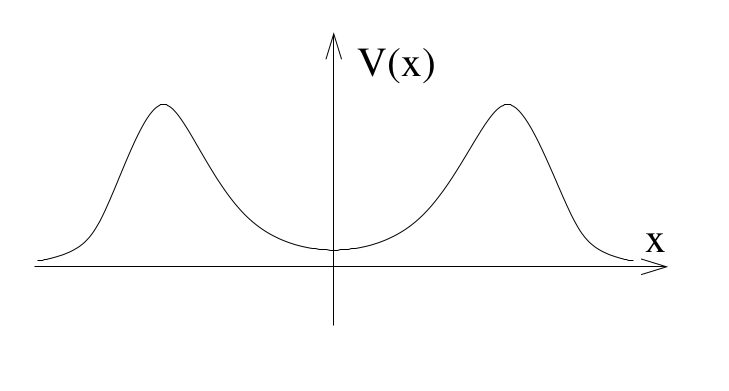
\includegraphics[scale=0.2]{QM/resonance0.png}
\caption{Example}
\end{figure} 
One the one hand, we know that there can be no bound states in such a trap because they will have $E > 0$. 
Any particle that we place in the trap will ultimately tunnel out. 
On the other hand, if the walls of the trap are very large then we might expect that the particle stays there for a long time before it eventually escapes. 
In this situation, we talk of a resonance. These are also referred to as unstable or metastable states.
\\ \\
Suppose that the S-matrix $S_{++}$ has a pole that lies on the complex momentum plane at position $k = k_0 - i\gamma$. We note that the energy is also imaginary
\[E = E_0 - i\frac{\Gamma}{2} , \quad E_0 \equiv \frac{k_0^2-\gamma^2}{2m} , \quad \Gamma \equiv \frac{2\gamma k_0}{m}.\]
Recall that the time dependence of the wave function is given by
\[e^{-iEt} = e^{-iE_0t}e^{-\Gamma t/2}.\]
For $\gamma > 0$, the overall form of the wave function decays exponentially with time. This is the characteristic behaviour of unstable states. 
A wave function that is initially supported inside the trap will be very small there at time much larger than $\tau = {1}/{\Gamma}$. Here $\tau$ is called the half-life of the state, while $\Gamma$ is usually referred to as the width of the state.
Including the time dependence, when $S_{++}\ \to \infty$, the solution takes the asymptotic form
\[\psi_+(x,t) = \begin{cases} e^{-iE_0t}e^{-ik_0x}e^{-\gamma x - \Gamma t/2} , \quad x\to -\infty \\  e^{-iE_0t}e^{ik_0x}e^{\gamma x - \Gamma t/2} , \quad x\to \infty \end{cases}.\]
The final factor varies as
\[e^{\pm\gamma(x\mp vt)} , \quad v = \frac{\Gamma}{2\gamma} = \frac{k_0}{m}.\]
This has the interpretation of a particle moving with momentum $-k_0$. This, of course, is the particle which has escaped the trap.
The upshot of this discussion is that poles of the S-matrix in the lower-half complex plane correspond to resonances. It is often useful to write $S_{++}$ as a function of energy rather than momentum. Since $S_{++}$ is a phase, close to a resonance it necessarily takes the form
\[S_{++} = \frac{E-E_0-i\Gamma/2}{E-E_0+i\Gamma/2}.\]


\section{Lippmann–Schwinger equation}
Imagine a particle coming in and getting scattered by a short-ranged potential $V(x)$ located around the origin $x \sim 0$. The time-independent Schr\"{o}dinger equation is simply
\[(H_0 + V)|\psi\rangle = E |\psi\rangle,\]
where $H_0 \equiv {p^2}/{2m}$ is the free-particle Hamiltonian operator. We can write the solution as
\[|\psi^{(\pm)}\rangle = \frac{1}{E-H_0 \pm i\epsilon}V|\psi^{(\pm)}\rangle + |\phi\rangle,\]
where $H_0 |\phi\rangle = E |\phi\rangle$. In coordinate representation,
\[\psi^{(\pm)}(\mathbf{x}) = \phi(\mathbf{x}) + \int d^3x' \langle \bm{x} | \frac{1}{E-H_0 \pm i\epsilon} | \bm{x}' \rangle V(\bm{x}') \psi^{(\pm)}(\bm{x}'),\]
where $\phi(\bm{x}) = e^{i\bm{k}\cdot\bm{x}} / (2\pi)^{\frac{3}{2}}$. Define the Green function as
\[G_{\pm}(\bm{x},\bm{x}') \equiv \frac{1}{2m} \langle \bm{x} | \frac{1}{E-H_0 \pm i\epsilon} | \bm{x}' \rangle.\]
We can derive that
\[G_{\pm}(\bm{x},\bm{x}') = -\frac{1}{4\pi} \frac{e^{\pm ik|\bm{x}-\bm{x}'|}}{|\bm{x}-\bm{x}'|},\]
where $k \equiv \sqrt{2mE}$. And it is easy to show that
\[(\nabla^2 + k^2)G_{\pm}(\bm{x},\bm{x}') = \delta(\bm{x}-\bm{x}').\]
Therefore, we have
\[\psi^{(\pm)}(\bm{x}) = \frac{e^{i\bm{k}\cdot\bm{x}}}{(2\pi)^{\frac{3}{2}}} - 2m \int d^3x' \frac{1}{4\pi} \frac{e^{\pm ik|\bm{x}-\bm{x}'|}}{|\bm{x}-\bm{x}'|} V(\bm{x}') \psi^{(\pm)}(\bm{x}').\]
We now can interpret $\psi^{+}(\bm{x})$ as a superposition of incident plane wave and scattered wave which propagate from scatterer to outside region. From now on, we will denote it as $\psi(\bm{x})$.
\\ \\
The experiment is done typically by placing the detector far away from the scatterer $|\bm{x}| \ll a$ where $a$ is the ``size'' of the scatterer. The integration over $\bm{x}'$, on the other hand, is limited within the ``size'' of the scatterer because of the $V(\bm{x}')$ factor. Therefore, we are in the situation $|\bm{x}| \ll |\bm{x}'|$, and hence can use the approximation
\[|\bm{x}-\bm{x}'| \approx |\bm{x}| - \frac{\bm{x}' \cdot \bm{x}}{|\bm{x}|},\]
Under this limit,
\[\psi(\bm{x}) = \frac{e^{i\bm{k}\cdot\bm{x}}}{(2\pi)^{\frac{3}{2}}} - 2m \frac{e^{ikr}}{4\pi r} \int d^3x' e^{-i\bm{k}' \cdot \bm{x}'} V(\bm{x}') \psi(\bm{x}').\]
where $r \equiv |\bm{x}|$ and $\bm{k}' \equiv k {\bm{x}}/{r}$. It is customary to write this equation in the form
\[\psi(\bm{x}) = \frac{1}{(2\pi)^{\frac{3}{2}}}\left( e^{i\bm{k}\cdot\bm{x}} +  f(\bm{k},\bm{k}') \frac{e^{ikr}}{r} \right) ,\]
where
\[f(\bm{k},\bm{k}') \equiv - \frac{m}{2\pi} (2\pi)^3  \langle \bm{k}'| V | \psi\rangle .\]
Recall the definition of cross section
\[\sigma \equiv \frac{\mbox{Number of Events}}{\mbox{Time} \times \mbox{Incident Flux}}.\]
Therefore, the differential cross section for particles being scattered into the solid angle is
\[d\sigma = \frac{|\bm{j}_{\mathrm{scatt}}| r^2 d\Omega}{|\bm{j}_{\mathrm{inc}}|} = |f(\bm{k},\bm{k}')|^2 d\Omega.\]
\\
In a more realistic situation, we should use wave packets to describe the scattering process. The basic picture is a free wave packet approaches the scattering center. After a long time, we have both the original wave packet moving in the original direction plus a spherical wave front that moves outward. The details can be found in the section 3 of the lecture notes 
\href{http://hitoshi.berkeley.edu/221B/index.html}{\emph{Scattering Theory I (Hitoshi Murayama)}}.
\\ \\
Furthermore, if we require that the normalization of the wave function should always satisfy $\int dx^3 |\psi(\bm{x})|^2 = 1$ for any $t$, as guaranteed by the unitarity of time evolution operator. This requirement leads to a special requirement on the scattered wave, and hence $f(\bm{k},\bm{k}')$, from witch we can derive the optical theorem.\\

\begin{newthem}[Optical theorem]
\[\mathrm{Im} f(\theta = 0) = \frac{k\sigma_{\mathrm{tot}}}{4\pi},\]
where
\[f(\theta = 0) \equiv f(\bm{k},\bm{k}).\]
The setting of $\bm{k} \equiv \bm{k}'$ imposes scattering in the forward direction, and
\[\sigma_{\mathrm{tot}} = \int \frac{d\sigma}{d\Omega} d\Omega.\]
\end{newthem}
\noindent
\\
The meaning of this theorem is clear. Because the scattered wave takes the probability away to different directions, the total probability for the particle to go to the forward direction (unscattered) should decrease. This decrease is caused by the interference between the unscattered and scattered waves and hence is proportional to ${\rm Im} f(0)$. On the other hand, the amount of decrease in the forward direction should equal the total probability at other directions, which is proportional to the total cross section. The proof can be found in the section 4 of the lecture notes \href{http://hitoshi.berkeley.edu/221B/index.html}{\emph{Scattering Theory I (Hitoshi Murayama)}}.

\section{Born approximation}
If $|\psi\rangle = |\phi\rangle + O(V)$ is close to $|\phi\rangle$, we can solve the Lippmanmn-Schwinger equation by perturbation theory. The lowest order approximation in $V$ is
\[|\psi\rangle = \frac{1}{E-H_0 + i\epsilon} V|\phi\rangle + |\phi\rangle.\]
This is called Born approximation. In coordinate representation,
\[f^{(1)}(\bm{k},\bm{k}') = - \frac{m}{2\pi} \int d^3x V(\bm{x}) e^{i\bm{q}\cdot\bm{x}},\]
where $\bm{q} \equiv \bm{k} - \bm{k}'$. If the potential is central, we can derive that
\[f^{(1)}(\bm{k},\bm{k}') = - \frac{2m}{q} \int_0^{\infty} dr \: r V(r) \sin(qr).\]

\subsubsection{Yukawa potential}
\[V = \frac{\alpha}{r}  e^{-\mu r}.\]
We can derive
\[f(\theta) = - \frac{2m\alpha}{q^2 + \mu^2}.\]
Differential cross section is therefore given by
\[\frac{d\sigma}{d\Omega} = (2m\alpha)^2 \frac{1}{[2k^2(1-\cos\theta) + \mu^2]^2}.\]
The total cross section is obtained by integrating over $d\Omega$,
\[\sigma = (2m\alpha)^2 \frac{4\pi}{4k^2\mu^2 + \mu^4}.\]

\subsubsection{Coulomb potential}
\[V = \frac{\alpha}{r}.\]
Take the limit $\mu \to 0$, we can get
\[f(\theta) = - \frac{2m\alpha}{q^2}.\]
Different cross section is given by
\[\frac{d\sigma}{d\Omega} = (\frac{\alpha}{4E})^2 \frac{1}{\sin^4{\frac{\theta}{2}}}.\]
The total cross section diverges. The divergence is in the $\cos\theta$ integral when $\theta \to 0$. In other words, the divergence occurs for the small momentum transfer $q \to 0$, which corresponds to large distances.
The reason why the total cross section diverges is because the Coulomb potential is actually a long-range force. No matter how far the incident particles are from the charge, there is always an effect on the motion of the particles and they get scattered.

\subsubsection{Form factor}
\noindent
If the source of Coulomb potential has an distribution $\rho_N(\bm{x})$, then
\[V(\bm{x}) = \int d^3x \frac{\alpha}{|\bm{x}-\bm{x}'|} \rho(\bm{x}').\]
Note that the potential is mathematically a convolution of the Coulomb potential and the probability density. Since the first Born amplitude is nothing but the Fourier transform of the potential, the convolution becomes a product of Fourier transforms, one for the Coulomb potential and the other for the probability density. Thus
\[f(\theta) = f(\theta)_{\mathrm{pointlike}} F(q),\]
where
\[F(q) \equiv \int d^3x \rho(\bm{x}) e^{i \bm{q} \cdot \bm{x}},\]
being called form factor.

\subsubsection{Born expansion}
\noindent
Define T-matrix by
\[V | \psi \rangle = T |\phi\rangle.\]
Using the definition of the T-matrix, we find
\[f(\bm{k},\bm{k}') = - \frac{m}{2\pi} (2\pi)^3  \langle \bm{k}'| T | \bm{k}\rangle .\]
Using the Lippmann–Schwinger equation and multiplying the
both sides by $V$ from left, we find
\[ T |\phi\rangle = V \frac{1}{E-H_0 + i\epsilon}T|\phi\rangle + V|\phi\rangle.\]
A formal solution to the T-matrix is
\[T = \frac{1}{1-V\frac{1}{E-H_0 + i\epsilon}}V.\]
By Taylor expanding this operator in geometric series, we find
\[T = V + V \frac{1}{E-H_0 + i\epsilon} V + V \frac{1}{E-H_0 + i\epsilon} V \frac{1}{E-H_0 + i\epsilon} V + \cdots\]
Thus
\[|\psi\rangle = \left( 1 +  \frac{1}{E-H_0 + i\epsilon} V +  \frac{1}{E-H_0 + i\epsilon} V \frac{1}{E-H_0 + i\epsilon} V + \cdots \right) | \phi \rangle.\]
The first term is the wave which did not get scattered.
The second term is the wave that gets scattered at a point in the potential and then propagates outwards by the propagator. 
In the third term, the wave gets scattered at a point in the potential, propagates for a while, and gets scattered again at another point in the potential, and propagates outwards. 
In the $n+1$-th term, there are $n$ times scattering of the wave before it propagates outwards.

\section{Partial wave analysis}
\subsubsection{Partial wave expansion}
When the potential is \textbf{central}, angular momentum is conserved due to Noether's theorem. Therefore, we can expand the wave function in the eigenstates of the angular momentum. Obtained waves with definite angular momenta are called partial waves. We can solve the scattering problem for each partial wave separately, and then in the end put them together to obtain the full scattering amplitude.
The plane wave can be expanded as follows.
\[e^{ikz} = \sum_{l=0}^{\infty}(2l+1)i^l j_l(kr) P_l(\cos \theta).\]
Here, $j_l(kr)$ is \href{https://en.wikipedia.org/wiki/Bessel_function#Spherical_Bessel_functions:_jn.2C_yn}{spherical Bessel functions} of first kind. The asymptotic behaviour of $j_l(kr)$ at large $r$ can be written as
\[j_l(kr) \sim \frac{\sin(kr-\frac{l\pi}{2})}{kr}.\]
Thus
\[e^{ikz} \sim \frac{1}{2ikr} \sum_{l=0}^{\infty} (2l+1) (e^{ikr} - (-1)^l e^{-ikr})P_l(\cos \theta).\]
Meanwhile, the $f$ factor can be expanded as
\[f(\theta) = \sum_{l=0}^{\infty} f_l (2l+1)P_l(\cos \theta).\]

\subsubsection{Optical theorem constraint}
\noindent
The cross section can be represented by expansion coefficient of $f$ factor as
\[\sigma = 4\pi \sum_l (2l+1)|f_l|^2.\]
On the other hand, 
\[\mathrm{Im} f(0) = \sum_l (2l+1) \mathrm{Im} f_l.\]
From optical theorem we can derive that
\[|f_l|^2 = \frac{1}{k} \mathrm{Im} f_l.\]
This constraint can be rewritten as
\[|1+2ikf_l|^2 = 1.\]
Thus we can define a phase $\delta_l$ as 
\[1+2ikf_l = e^{2i\delta_l},\]
or equivalently,
\[f_l = \frac{1}{k} e^{i\delta_l} \sin(\delta_l).\]

\subsubsection{Phase shifts}
\noindent
We can derive the asymptotic behaviour of the wave function as
\[\psi(\bm{x}) \sim \frac{1}{2ikr} \sum_{l} (2l+1)P_l(\cos \theta) [e^{ikr}e^{2i\delta_l} - (-1)^l e^{-ikr}].\]
Compare it to the case of the plane wave without scattering. What this equation says is that the wave converging on the scatterer
has the well-defined phase factor $-(-1)^l$, the same as in the case without scattering. On the other hand, the wave that emerges from the scatterer has an additional phase factor $e^{2i\delta_l}$. All what scattering did is to shift the phase of the emerging wave by $2\delta_l$. The reason why this is merely a phase factor is
the conservation of probability. What converged to the origin must come out with the same strength. But this shift in the phase causes the interference among all partial waves different from the case without the phase shifts, and the result is not a plane wave but contains the scattered wave.
In terms of the phase shifts, the cross section is given by
\[\sigma = \frac{4\pi}{k^2} \sum_l (2l+1) \sin^2\delta_l.\]
Actual calculation of phase shifts is basically to solve the Schr\"{o}dinger equation for each partial waves,
\[\left[-\frac{1}{r}\frac{d^2}{dr^2}r+\frac{l(l+1)}{r^2}+2mV(r)\right]R_l(r) = k^2 R_l(r).\]
After solving the equation, we take the asymptotic limit $r \to \infty$, and write $R_l(r)$ as a linear combination of $j_l(kr)\cos \delta_l - n_l(kr) \sin \delta_l $. The relative coefficients of $j_l$ and $n_l$ determines the phase shift $\delta_l$, and hence the cross section.

\subsubsection{Hard sphere scattering}
The potential for hard sphere scattering is
\[V = \begin{cases} 0 , \quad (r > a) \\ \infty , \quad (r < a)\end{cases}.\]
The infinite potential corresponds to the boundary condition $R_l(a) = 0$. We first analyze the S-wave ($l = 0$). The Schr\"{o}dinger equation is simply 
\[-\frac{d^2 rR_0(r)}{dr^2} = k^2 rR_0(r).\]
The solution is
\[rR_0(r) = c\sin(k(r-a)) = \frac{ce^{ika}}{2i} \left[ e^{i(kr-2ka)} - e^{-ikr} \right].\]
Thus we have $\delta_0 = -ka$. The reason behind the phase shift is that the wave cannot penetrate into $r < a$, the wave is shifted outwards, which is the shift in the phase $-ka$. The cross section from the S-wave scattering is
\[\sigma_0 = \frac{4\pi}{k^2}\sin^2 ka.\]
Let us generalize the discussion to the case of a little bit penetrable potential
\[V = \begin{cases} 0 , \quad (r > a) \\ V_0 , \quad (r < a)\end{cases}.\]
Define $K^2 \equiv 2mV_0$. If $k > K$, we have
\[rR_0 = \begin{cases} \sin \sqrt{k^2-K^2}r , \quad (r < a) \\ \sin(kr+\delta_0) , \quad (r > a)\end{cases}.\]
By matching the logarithmic derivatives of the wave function at $r = a$, we find
\[\delta_0 = \tan^{-1} \left[\frac{k}{\sqrt{k^2-K^2}} \tan\sqrt{k^2-K^2}a \right]-ka.\]
For $k \gg K$, one can neglect $K$ and the phase shift vanishes. The energy is too large to care the slight potential and there is no scattering any more.
\\ \\
If $k < K$, we have
\[rR_0 = \begin{cases} \sinh \sqrt{K^2-k^2}r , \quad (r < a) \\ \sin(kr+\delta_0) , \quad (r > a)\end{cases}.\]
The phase shift is obtained as
\[\delta_0 = \tan^{-1} \left[\frac{k}{\sqrt{K^2-k^2}} \tanh\sqrt{K^2-k^2}a \right]-ka.\]
For $k \ll K$, we have
\[\delta_0 \sim ka \left[ \frac{1}{Ka} \tanh Ka - 1 \right].\]
The phase shift $\delta_0$ always starts linearly with $k$ at small momentum, and the slope is negative. This is a completely general result for a repulsive potential, and a convenient quantity
\[a_0 = \lim_{k \to 0} -\frac{d\delta_0}{dk}\]
is called the scattering length, as it has the dimension of the length. This quantity basically measures how big the scatterer is. The cross section at $k \to 0$ limit is then given by $4\pi a_0^2$ . For the hard sphere potential, the scattering length is indeed the size of the sphere.
\\ \\
For the hard sphere problem, the phase shifts for higher partial waves can be worked out similarly. We have
\[\tan\delta_l = \frac{j_l(ka)}{n_l(ka)}.\]
The cross section is then given by
\[\sigma = \frac{4\pi}{k^2} \sum_l (2l+1) \sin^2\delta_l = \sum_{l=0}^{\infty} \frac{4\pi(2l+1)}{k^2} \frac{[j_l(ka)]^2}{[j_l(ka)]^2+[n_l(ka)]^2}.\]
For small momenta $k \ll a^{-1}$, we can use the power expansion of the spherical Bessel function
\[j_l(r) \sim \frac{r^{l}}{(2l+1)!!} , \quad n_l(r) \sim -\frac{(2l-1)!!}{r^{l+1}},\]
and get that
\[\delta_l \sim (ka)^{2l+1}.\]
Thus phase shift (and so cross section) is smaller for higher partial waves. This is easy to understand. When $k$ is small, the centrifugal barrier does not allow the particle to reach $r=a$ classically. Therefore the effect of the potential is extremely suppressed.
On the other hand at high momenta, $\sin^2\delta_l$ oscillates between $0$ and $1$ as a function of $l$ up to $l \sim ka$. Above this value, the phase shift drops rapidly to zero. This makes sense from the classical physics intuition. When $l > ka$,
the impact parameter is larger than the size of the target and there should not be any scattering.

\section{Resonance}
\subsection{Attractive potential}
As for attractive potential scattering
\[V = \begin{cases} 0 , \quad (r > a) \\ -V_0 , \quad (r < a)\end{cases},\]
the phase shift for S-wave is
\[\delta_0 = \tan^{-1} \left[\frac{k}{\sqrt{k^2+K^2}} \tan\sqrt{k^2+K^2}a \right]-ka.\]
The scattering length is
\[a_0 = a\left[ 1 - \frac{\tan Ka}{Ka} \right] .\]
For small $K$, the scattering length is negative. This is easy to understand because the wave is pulled into the potential rather pushed out unlike the repulsive case. However, once we
make the potential more attractive (larger $K$), the scattering length grows and becomes even infinite at $Ka = {\pi}/{2}$.
\\ \\
Let us study the analytic structure of the scattering amplitude more carefully. We have
\[e^{2i\delta_0} = e^{-2ika} \frac{1 + i \frac{k}{\sqrt{k^2+K^2}} \tan\sqrt{k^2+K^2}a}{1 - i \frac{k}{\sqrt{k^2+K^2}} \tan\sqrt{k^2+K^2}a}.\]
It can have a pole if
\[1 - i \frac{k}{\sqrt{k^2+K^2}} \tan\sqrt{k^2+K^2}a = 0.\]
This equation appears impossible to satisfy, but it can be on the complex plane of $k$. For a pure imaginary $k = i\kappa$, the equation becomes
\[\kappa = - \frac{\sqrt{K^2-\kappa^2}}{\tan \sqrt{K^2-\kappa^2}a}.\]
This is the condition for bound states (the scattering wave $e^{ikr}$ becomes $e^{-\kappa r}$, which is trapped by scatter). By decreasing $K$ from a sufficiently large value with bound states, the bound state energies $E = -{\kappa^2}/{2m}$ move up. When $Ka = (n + \frac{1}{2})\pi$, $\tan Ka \to \infty$, and we find a bound state approaching $\kappa = k = 0$. 
This is when the scattering length diverges. In other words, the infinite scattering cross section at $k = 0$ happens because there is a bound state exactly at $ k = 0$.
\\ \\
This can also be seen on the complex $k$ plane in the following manner. The lower half plane is unphysical as it corresponds to an exponentially growing wave function at the infinity for the scattered wave. 
When there are bound states, we see poles along the positive imaginary axis. By decreasing $K$, the poles along the positive imaginary axis go down, and a pole reaches the origin. 
By further decreasing $K$, the pole goes below the origin into the unphysical region. 
However, the existence of a pole just below the origin makes the scattering amplitude at $k \to 0$ large and results in an anomalously large cross section. 

\subsection{Delta-shell potential}
As for delta shell scattering
\[V = \gamma\delta(r-a),\]
the phase shift for S-wave is
\[e^{2i\delta_0} = e^{-2ika}\frac{\sin ka + \frac{k}{2m\gamma}e^{ika}}{\sin ka + \frac{k}{2m\gamma}e^{-ika}}.\]
The pole satisfies that
\[e^{2ika} = 1 - 2i\frac{k}{2m\gamma}.\]
When $\gamma$ is large, we can get
\[k \approx \frac{n\pi}{a + \frac{1}{2m\gamma}} -i \left(\frac{1}{2m\gamma} \right)^2 \frac{n^2\pi^2}{a^3} + O(\gamma^{-2}).\]
The poles are in the unphysical lower half plane. But when $\gamma$ is large, the poles are very close to the real axis, and the scattering amplitude receives a large enhancement due to these poles. 
In the limit of $\gamma \to \infty$, or in other words in the limit of no coupling between the regions inside and outside the shell, they become poles along the real axis. 
They are the discrete states inside the shell in this limit. 
By making $\gamma$ finite, we introduce coupling between the discrete states inside the shell to the continuum states outside the shell.
\\ \\
It is instructive to solve Schr\"{o}dinger equation for the values of $k$ which correspond to the location of poles. Because the outgoing wave $e^{ikr}$ is enhanced relative to the incoming wave $e^{-ikr}$ by an infinite amount due to the pole, the boundary condition is that the solution is ``purely outgoing'', i.e.
\[rR_0 = \begin{cases} \sin kr , \quad (r<a) \\ \sin ka e^{ik(r-a)} , \quad (r>a)  \end{cases} , \quad \mathrm{Re}(k) > 0.\]
Because the factor $e^{ik(r-a)}$ grows exponentially at large $r$ due to the negative imaginary part in $k$, the solution is not a regular normalizable solution.
In the large $\gamma$ limit, $\sin ka \sim O(\gamma^{-1})$ is small. Therefore the wave function almost vanishes at the shell.
Outside the shell, the wave function oscillates at the small amplitude $\sin(ka)$, which however starts growing again due to the $e^{ik(r-a)}$ factor exponentially.
\\ \\
We now put the time dependence in. The energy eigenvalue
is $E = {k^2}/{2m}$, where $k$ is at the pole. If the pole is at
\[k = k_0 - i\kappa,\]
the energy eigenvalue is at
\[E = E_0 - i\frac{\Gamma}{2} = \frac{k_0^2}{2m} - i \frac{k_0\kappa}{m} + O(\kappa^2).\]
For instance in the large $\gamma$ limit
\[E \sim \frac{1}{2m} \left( \frac{n\pi}{a + \frac{1}{2m\gamma}}\right)^2 - i \left( \frac{n\pi}{2ma}\right)^3 \frac{2}{\gamma^2 a} + O(\gamma^{-3}).\]
The time dependence of the wave function is simply
\[rR_0(r,t) = rR_0(r) e^{-iE_0t} e^{-\frac{\Gamma t}{2}} = \begin{cases} \sin kr \, e^{-iE_0t} e^{-\frac{\Gamma t}{2}} , \quad (r<a) \\\sin ka \,  e^{ik(r-a)} e^{-iE_0t} e^{-\frac{\Gamma t}{2}} , \quad (r > a) \end{cases}.\]
Inside the shell, it shows an exponentially decaying probability density uniformly over space.
Outside the shell, the probability density is $|rR_0|^2 \propto e^{2\kappa r-\Gamma t}$ , which shows the probability flowing out to infinity with speed $\Gamma/2\kappa = {k_0}/{m}$,
nothing but the velocity of the particle itself. In other words, the wave function describes a ``bound state'' inside shell decaying into a continuum state outside the shell moving away at the expected velocity. The resonances can be viewed as
quasi-bound states which decay into continuum states. The lifetime of the quasi-bound states is $\tau = {1}/{\Gamma}$.
A more rigorous treatment of resonance using wave packets can be found in the section 5 of the lecture notes 
\href{http://hitoshi.berkeley.edu/221B/index.html}{\emph{Scattering Theory III (Hitoshi Murayama)}}.

\subsection{General description of resonances}
In general, once we know that there is a pole just below the real axis, we can approximate the phase shift by the contribution from the pole only, ignoring a continuum:
\[e^{2i\delta_l} \sim \frac{g(E)}{E-E_0 + i\Gamma/2}.\]
Because of the unitarity $|e^{2i\delta_l}|^2 = 1$ , we immediately conclude
\[ e^{2i\delta_l} \sim e^{2i\theta}\frac{E-E_0-i\Gamma/2}{E-E_0 + i\Gamma/2} .\]
Ignoring the continuum contribution $e^{2i\theta}$,
\[\sin^2 \delta_l = \frac{\Gamma^2/4}{(E-E_0)^2+\Gamma^2/4}.\]
\begin{figure}[!h]
	\centering
	\includegraphics[height=4cm ,width=6.23cm]{QM/resonance.png}
	\caption{Resonance curve}
\end{figure}\\
We then can establish the relationship between the life time of the quasi-bound state and the FWHM of the resonance
\[\tau \Delta E \sim 1.\]

\section{Two-to-two scattering}
Similar to the discussion in hydrogen atom, we take as independent variables the center of mass and relative coordinates of the particles
\[\bm{X} = \frac{m_1\bm{x}_1 + m_2\bm{x}_2}{m_1+m_2} , \quad \bm{x} = \bm{x}_1-\bm{x}_2.\]
The corresponding momentum operators are
\[\bm{P} = \bm{p}_1 + \bm{p}_2 , \quad \bm{p} = \frac{m_1\bm{p}_1-m_2\bm{p}_2}{m_1 + m_2}.\]
Then the Hamiltonian becomes
\[H = \frac{P^2}{2M} + \frac{p^2}{2\mu} + V(|\bm{x}|).\]
Then the problem reduces to the potential scattering problem for a particle of mass $\mu = m_1m_2/(m_1+m_2)$.
\\ \\
If two particles that scatter are identical particles, such as electron-electron scattering or scattering of two identical atoms, symmetry of the wave function needs to be considered.
Under the interchange of two particles, the center of mass motion is not affected, but the relative coordinates change their signs. If they have spins, their spins need to be interchanged at the same time.
\\ \\
If two particles are identical spinless bosons, there is no spin degrees of freedom and the interchange of particles is simply $\bm{x} \to -\bm{x}$ in the wave function. 
Because they are bosons, the wave function should not change under the interchange of particles, and hence the wave function must be an even function of $\bm{x}$. 
Therefore the asymptotic form of the wave function must be changed to
\[\psi(\bm{x}) \to e^{ikz} + e^{-ikz} + [f(\theta) + f(\pi - \theta)] \frac{e^{ikr}}{r}.\]
The differential cross section is then found to be
\[\frac{d\sigma}{d\Omega} = |f(\theta)+f(\pi-\theta)|^2.\]
Note that one should not integrate over the entire solid angle to obtain the total cross section because $(\theta,\phi)$ and $(\pi - \theta,\phi+\pi)$ correspond to an identical state.
For two spin ${1}/{2}$ fermions, there are two possible spin wave functions, symmetric $S = 1$ and anti-symmetric $S = 0$.
Therefore depending on the spin wave function, we either have a anti-symmetric or symmetric spatial wave function, respectively. In particular, the differential cross section is the same as the spinless bosons for the anti-symmetric spin wave function $S= 0 $ while it is
\[\frac{d\sigma}{d\Omega} = |f(\theta) - f(\pi-\theta)|^2.\]
for the symmetric spin wave function $S = 1$.

\section{Time-dependent formulation}
Recall the time-dependent perturbation theory, the rate of the initial state $|i\rangle$ to transform to the final state $|f\rangle$ to the first order in perturbation $V$ is
\[\Gamma(i \to f) = 2\pi \delta(E_{\mathrm{i}}-E_{\mathrm{f}}) |V_{\mathrm{fi}}|^2.\]
When applied to the scattering problem, an additional issue is to define how we sum over the final states. 
In particular, we would like to sum over the continuum plane-wave states, and we must make the sum well-defined.
To define the sum over the continuum states, it is useful to consider the system in a cube of size $L$. 
We impose the periodic boundary condition. The plane-wave solutions in this box are given by
\[\psi_{n_x,n_y,n_z}(\bm{x}) = \frac{1}{L^{3/2}} e^{2\pi i(n_x x + n_y y + n_z z)/L}.\]
In the limit $L \to \infty$, we have
\[\sum_{n_x,n_y,n_z} = \left( \frac{L}{2\pi}\right)^3 \sum_{n_x,n_y,n_z} \left( \frac{2\pi}{L}\right)^3 \to \left( \frac{L}{2\pi}\right)^3 \int d\bm{p} = \int \frac{d\bm{x}d\bm{p}}{(2\pi)^3}.\]
Coming back to the scattering problem, we sum over the final states to define the probability of the outgoing particle to go into various momentum states
\[\sum_{f} \Gamma(i \to f) = \int \frac{L^3 d\bm{p}}{(2\pi)^3} 2\pi \delta(E_{\mathrm{i}}-E_{\mathrm{f}}) |V_{\mathrm{fi}}|^2.\]
Note that
\[V_{\mathrm{fi}} = \int d\bm{x} \frac{e^{-i\bm{p}_{\mathrm{f}} \cdot \bm{x}}}{L^{3/2}} V(\bm{x}) \frac{e^{i\bm{p}_{\mathrm{i}} \cdot \bm{x}}}{L^{3/2}}  = \frac{1}{L^3} \int d\bm{x} V(\bm{x}) e^{i\bm{q}\cdot\bm{x}},\]
where $\bm{q} = \bm{p}_{\mathrm{i}} - \bm{p}_{\mathrm{f}}$.
Since the incident flux of the incoming particle is ${v}/{L^3}$, the cross section is
\[\sigma = \frac{L^3}{v} \sum_{f} \Gamma(i \to f) =  \frac{m}{p_{\mathrm{i}}} \int \frac{ d\bm{p}}{(2\pi)^3} 2\pi \delta(E_{\mathrm{i}}-E_{\mathrm{f}}) \left |\int d\bm{x} V(\bm{x}) e^{i\bm{q}\cdot\bm{x}} \right|^2.\]
Note that $E = {p^2}/{2m}$ and $\delta(E_{\mathrm{i}}-E_{\mathrm{f}}) = {m} \delta(p_{\mathrm{f}}-p_{\mathrm{i}})/{p_{\mathrm{i}}}$, finally we can get
\[\sigma = \int d\Omega \left | \frac{m}{2\pi} \int d\bm{x} V(\bm{x}) e^{i\bm{q}\cdot\bm{x}} \right|^2.\]
This is nothing but the Born approximation for the cross section.
\part{Quantum Field Theory}
\chapter{From Classical Field to Quantum Field}
\section{Motivation}
The state of a field is described by an element $|\psi\rangle$ in Hilbert space. The measurement of the field is realised by an operator field $\phi_a(\bm{x})$. The mean value of the measurement of the field satisfies Erenfest's theorem
\[\frac{d\langle \psi| \phi_a(\bm{x}) | \psi \rangle}{dt} = -i \langle \psi | [\phi_a(\bm{x}),H_{\rm S}] | \psi \rangle.\]
If $[\phi_a(\bm{x}),H_{\rm S}]_Q = i[\phi_a(\bm{x}),H_{\rm S}]_C$, classical field theory will be an average effect of quantum field theory. We also note that the commutation relation here $[A,B] = AB - BA$ obeys the same operation laws as the Poisson bracket in classical field theory. Therefore, what we need here is
\begin{enumerate}
\item the canonical quantization
\[[\phi_a(\bm{x}),\phi_b(\bm{y})] = 0 , \quad [\pi^a(\bm{x}),\pi^b(\bm{y})] = 0 , \quad [\phi_a(\bm{x}),\pi^b(\bm{y})] = i \delta_a^b \delta(\bm{x}-\bm{y}) ,\]
\item the same definition of $\mathcal{L}$,$\pi^a$ and $H$ as those in corresponding classical theory.
\end{enumerate}
In Heisenberg picture, we define
\[A_{\rm H} \equiv U^{-1}(t,t_0) A_{\rm S} U(t,t_0).\]
Especially, we have
\[\phi_a(x) \equiv U^{-1}(t,t_0) \phi_a(\bm{x}) U(t,t_0),\]
\[\pi^a(x) \equiv U^{-1}(t,t_0) \pi^a(\bm{x}) U(t,t_0).\]
If $A = f(\phi_a(\bm{x}),\pi^a(\bm{x}),t)$, then $A_{\rm H} = f(\phi_a(x),\pi^a(x),t)$.
Thus the canonical quantization can be generalized to the field operator in any time
\[[\phi_a(\bm{x},t),\phi_b(\bm{y},t)] = 0 , \quad [\pi^a(\bm{x},t),\pi^b(\bm{y},t)] = 0 , \quad [\phi_a(\bm{x},t),\pi^b(\bm{y},t)] = i \delta_a^b \delta(\bm{x}-\bm{y}) .\]
The dynamics of the field can be describe by Heisenberg equation
\[\frac{d\phi_a(x)}{dt} = -i[\phi_a(x),H_{\rm H}],\]
\[\frac{d\pi^a(x)}{dt} = -i[\pi^a(x),H_{\rm H}],\]
whose form will be equivalent to the classical field equation.

\section{Lorentz invariance in quantum field theory}
\[| \bar{\psi}\rangle = U(\Lambda)| \psi\rangle.\]
Scalar fields:
\[\langle \bar{\psi} | \phi(x) | \bar{\psi}\rangle = \langle \psi | \phi(\Lambda^{-1}x) | \psi\rangle.\]
\[U^{-1}(\Lambda) \phi(x) U(\Lambda) = \phi(\Lambda^{-1}x).\]
Vector fields:
\[\langle \bar{\psi} | A^{\mu}(x) | \bar{\psi}\rangle = \langle \psi | \Lambda^{\mu}_{\phantom{\mu}\nu} A^{\nu}(\Lambda^{-1}x) | \psi\rangle.\]
\[U^{-1}(\Lambda) A^{\mu}(x) U(\Lambda) = \Lambda^{\mu}_{\phantom{\mu}\nu} A^{\nu}(\Lambda^{-1}x).\]
Lorentz invariance means Lagrangian must be a scalar, or more loosely, action must be invariant under Lorentz transformation.

\section{Symmetry and conservation law}
Thanks to canonical quantization, equations in classical field theory will hold antomatically in quantum field theory as long as we interpret the field in equations as operators in Heisenberg picture. As a result, Noether's theorem holds in quantum field theory as well. 
If the infinitesimal transformation of the field
\begin{equation}
    \phi_a \to \phi_a + \delta \phi_a, \quad  \mathcal{L} \to \mathcal{L} + \delta \mathcal{L},
\end{equation}
satisfy the condition $\delta L = \partial_{\mu} K^{\mu}$, we have the conserved current
\begin{equation}
    j^{\mu} = - \frac{\partial \mathcal{L}}{\partial (\partial_{\mu} \phi_a)}\delta \phi_a + K^{\mu},
\end{equation}
which satisfies the continuity equation $\partial _{\mu} j^{\mu} = 0$. 
Integrating the continuity equation over a volume $V$, large enough to have no net currents through its surface, leads to the conservation law
\begin{equation}
    \frac{d Q}{dt} = 0,
\end{equation}
where $Q = \int_{V} j^0 dV$. 
Furthermore, we can prove that $Q$ is the generator of the infinitesimal transformation. i.e.
\begin{equation}
    U^{\dagger} \phi_a U = \phi_{a} + \delta \phi_{a},
\end{equation}
where $U \equiv e^{iQ} = I + iQ$.
\\ \\
However, in some cases, classical conservation laws would break in quantum field theory, called anomalies. It will be introduced in section 27.4.

\section{Momentum}
\noindent
The definition and conservation of momentum is the same as that in classical theory:
\[T^{\mu \nu} \equiv -\frac{\partial \mathcal{L}}{\partial(\partial_{\mu}\phi_a)} \partial^{\nu} \phi_a + \eta^{\mu \nu} \mathcal{L} , \quad \partial_{\mu} T^{\mu \nu} = 0.\]
\[P^{\mu} \equiv \int T^{0 \mu} d^3 x \left(P^{0} = H, P^{i} = \int -\pi^a \partial^i \phi_a d^3 x \right), \quad \frac{d P^{\mu}}{dt} = 0. \]
We can get the commutation relation
\begin{eqnarray}
\left[\phi_a,P^{\mu}\right] &=& -i\partial^{\mu} \phi_a, \nonumber \\
\left[\pi^a,P^{\mu}\right] &=& -i\partial^{\mu} \pi^a, \nonumber \\
\left[P^{\mu},P^{\nu}\right] &=& 0 ,\nonumber 
\end{eqnarray}
We define the translation operator $T(s)$ by
\[T^{-1}(s) \phi_a(x) T(s) = \phi_a(x-s).\]
Then we can derive that
\[T(\epsilon) = 1 - i\epsilon_{\mu} P^{\mu} , \quad T(s) = e^{-iP^{\mu}s_{\mu}}.\]

\section{Angular Momentum}
\noindent
The definition and conservation of angular momentum is the same as that in classical theory:
\[M^{\mu \nu \rho} \equiv x^{\nu}T^{\mu \rho} - x^{\rho} T^{\mu \nu} - \frac{\partial \mathcal{L}}{\partial (\partial_{\mu}\phi_a)}(\Sigma^{\nu \rho})_{a}^{\phantom{a}b}\phi_b.\]
\[M^{\nu \rho} \equiv \int M^{0 \nu \rho} d^3 x = \int (x^{\mu}T^{0\nu}-x^{\nu}T^{0\mu}-\pi^a(\Sigma^{\mu \nu})_{a}^{\phantom{a}b}\phi_b) d^3 x, \quad \frac{dM^{\nu \rho}}{dt} = 0.\]
We also define that
\[M_{\rm L}^{\mu \nu} \equiv \int (x^{\mu}T^{0\nu}-x^{\nu}T^{0\mu}) d^3 x , \quad M_{\rm S}^{\mu \nu} \equiv\int (-\pi^a(\Sigma^{\mu \nu})_{a}^{\phantom{a}b}\phi_b) d^3 x,\]
\[(\mathcal{L}^{\mu \nu})_a^{\phantom{a}b} \equiv -i(x^{\mu}\partial^{\nu}-x^{\nu}\partial^{\mu})\delta_a^{\phantom{a}b} , \quad (\mathcal{S}^{\mu \nu})_a^{\phantom{a}b} \equiv -i(\Sigma^{\mu \nu})_a^{\phantom{a}b}.\]
We can get the following commutation relation:
\[[\phi_a,M_{\rm L}^{\mu \nu}] = (\mathcal{L}^{\mu \nu})_a^{\phantom{a}b} \phi_b , \quad [\phi_a,M_{\rm S}^{\mu \nu}] = (\mathcal{S}^{\mu \nu})_a^{\phantom{a}b} \phi_b.\]
\[[\pi^a,M_{\rm L}^{\mu \nu}] = (\mathcal{L}^{\mu \nu})_b^{\phantom{b}a}\pi^{b}  , \quad [\pi^a,M_{\rm S}^{\mu \nu}] = - (\mathcal{S}^{\mu \nu})_b^{\phantom{b}a} \pi^b .\]
\[[M^{\mu \nu},M^{\rho \sigma}] = i(-\eta^{\nu \rho}M^{\mu \sigma} + \eta^{\sigma \mu}M^{\rho \nu} + \eta^{\mu \rho}M^{\nu \sigma} - \eta^{\sigma \nu}M^{\rho \mu}).\]
We again define $J_i \equiv \frac{1}{2} \epsilon_{ijk} M^{jk}$ and $K_i \equiv M^{i0}$. Commutation relations can be rewritten as
\begin{eqnarray}
\left[J_i,J_j\right] &=& i\epsilon_{ijk}J_k ,\nonumber \\
\left[J_i,K_j\right] &=& i\epsilon_{ijk}K_k ,\nonumber \\
\left[K_i,K_j\right] &=& -i\epsilon_{ijk}J_k .\nonumber
\end{eqnarray}
Further more, we have
\[[P^{\mu},M^{\rho \sigma}] = i(\eta^{\mu \sigma}P^{\mu} - \eta^{\mu \rho}P^{\sigma}),\]
i.e.
\begin{eqnarray}
\left[J_i,H\right] &=& 0 \nonumber \\
\left[J_i,P_j\right] &=& i\epsilon_{ijk}P_k \nonumber \\
\left[K_i,H\right] &=& iP_i \nonumber \\
\left[K_i,P_j\right] &=& i\delta_{ij}H \nonumber
\end{eqnarray}
We define $L_i \equiv \frac{1}{2} \epsilon_{ijk} M_{\rm L}^{jk}$ and $S_i \equiv \frac{1}{2} \epsilon_{ijk} M_{\rm S}^{jk}$. Then we have
\begin{eqnarray}
\left[L_i,S_j\right] &=& 0 ,\nonumber \\
\left[S_i,P_j\right] &=& 0 ,\nonumber \\
\left[L_i,P_j\right] &=& i\epsilon_{ijk}P_k .\nonumber
\end{eqnarray}
We define the rotation operator $U(\Lambda)$ by
\[U^{-1}(\Lambda) \phi_a(x) U(\Lambda) = \mathscr{S}_{a}^{\phantom{a}b}\phi_b(\Lambda^{-1}x),\]
where
\[\mathscr{S}_{a}^{\phantom{a}b} = \delta_{a}^{\phantom{a}b}+\frac{i}{2} \delta \omega_{\alpha \beta} (\mathcal{S}^{\alpha \beta})_{a}^{\phantom{a}b} .\]
We can derive that
\[U(1+\delta \omega) = 1 + \frac{i}{2} \delta \omega_{\mu \nu} M^{\mu \nu} , \quad U(\Lambda) = e^{\frac{i}{2} \theta_{\mu \nu} M^{\mu \nu}},\]
\[U^{-1}(\Lambda) P^{\mu} U(\Lambda) = \Lambda^{\mu}_{\phantom{\mu}\nu} P^{\nu}, \quad U^{-1}(\Lambda) M^{\mu \nu} U(\Lambda) = \Lambda^{\mu}_{\phantom{\mu}\rho} \Lambda^{\nu}_{\phantom{\nu}\sigma}M^{\rho \sigma}.\]

\section{Anticommutation relation}
\noindent
We define the anticommutation relation of operators as $\{A,B\} \equiv AB + BA$. Suppose that the field operator and its canonical momentum operator has the following anticommutation relation
\[\{\phi_a(\bm{x},t),\phi_b(\bm{y},t)\} = 0 , \quad \{\pi^a(\bm{x},t),\pi^b(\bm{y},t)\} = 0 , \quad \{\phi_a(\bm{x},t),\pi^b(\bm{y},t)\} = i \delta_a^b \delta(\bm{x}-\bm{y}) .\]
If the operator $A$ composes of the terms like $\pi^a \mathcal{E}_a^{\phantom{a}b} \phi_b$, we can show that the value of $[\phi_a,A]$ and $[\pi^a,A]$ is the same as those in the theory quantized with commutation relation. It is easy to verify that the operator $P^i$ and $M_{\rm S}^{\mu \nu}$ has the required form. The form of $H$ is determined by the specific theory. As we can see later, the Hamiltonian of Dirac field  has the required form. When it is quantized with anticommutation relation, the commutation relation between field operator and momentum, angular momentum discussed in previous section will be hold automatically. 

\chapter{Spin 0 Field}
\section{Klein-Gordon field}
\subsubsection{Lagrangian}
\[\mathcal{L} = -\frac{1}{2} \partial^{\mu} \phi \partial_{\mu} \phi -\frac{1}{2}m^2 \phi^2 + \Omega_0.\]

\subsubsection{Field equation}
\[(\partial^{\mu} \partial_{\mu} - m^2) \phi = 0.\]

\subsubsection{Hamiltonian}
\[\pi = \dot{\phi}.\]
\[\mathcal{H} = \frac{1}{2} \pi^2 + \frac{1}{2} (\nabla \phi)^2 + \frac{1}{2} m^2 \phi^2-\Omega_0.\]
\[H = \int \mathcal{H} d^3 x.\]

\subsubsection{Momentum and angular momentum}
\[T^{\mu \nu} = \partial^{\mu} \phi \partial^{\nu} \phi - \eta^{\mu \nu}(\frac{1}{2}\partial^{\mu}\phi \partial_{\mu} \phi + \frac{1}{2}m^2 \phi^2 -\Omega_0).\]
\[P^0 = H , \quad P^i = \int -\pi \nabla^i \phi d^3 x.\]
\[J_i = \int  \epsilon_{ijk} x^{j} \left(- \pi \nabla^{k} \phi\right) d^3 x.\]

\section{Canonical quantization Formulation}
\subsubsection{Canonical quantization}
\begin{eqnarray}
\left[\phi(\bm{x},t),\phi(\bm{y},t)\right] &=& 0 ,\nonumber \\
\left[\pi(\bm{x},t),\pi(\bm{y},t)\right] &=& 0 ,\nonumber \\
\left[\phi(\bm{x},t),\pi(\bm{y},t)\right] &=& i \delta(\bm{x}-\bm{y}) .\nonumber
\end{eqnarray}

\subsubsection{Fourier expansion}
\[\phi(\bm{x},t) = \int \widetilde{dk} \left[ a(\bm{k})e^{ikx} + a^{\dagger}(\bm{k})e^{-ikx} \right],\]
\[\pi(\bm{x},t) = -i \int  \widetilde{dk} \omega \left[ a(\bm{k})e^{ikx} - a^{\dagger}(\bm{k})e^{-ikx} \right],\]
where $k^2 \equiv \bm{k}^2 - \omega^2 = -m^2$, $kx \equiv \bm{k}\cdot \bm{x} - \omega t$, $\widetilde{dk} \equiv {d^3k}/{(2\pi)^3 2\omega}$. 
We can derive that
\[a(\bm{k}) = \int d^3 x e^{-ikx}(i\pi+\omega \phi),\]
\[a^{\dagger}(\bm{k}) = \int d^3 x e^{ikx}(-i\pi+\omega \phi).\]
We can also get the commutation relations in terms of $a$ and $a^{\dagger}$,
\begin{eqnarray}
\left[a(\bm{p}),a(\bm{q})\right] &=& 0 ,\nonumber \\
\left[a^{\dagger}(\bm{p}),a^{\dagger}(\bm{q})\right] &=& 0, \nonumber \\
\left[a(\bm{p}),a^{\dagger}(\bm{q})\right] &=& (2\pi)^3 2\omega \delta(\bm{p}-\bm{q}) .\nonumber
\end{eqnarray}

\subsubsection{Operator represented by $a$ and $a^{\dagger}$}
\[H=\int \widetilde{dk}\, \omega\, a^{\dagger}(\bm{k})a(\bm{k}) + (\mathcal{E}_0 - \Omega_0)V , \quad \mathcal{E}_0 = \frac{1}{2}(2\pi)^{-3}\int d^3 k \,\omega.\]
\[P^{i}=\int \widetilde{dk}\, k^{i}\, a^{\dagger}(\bm{k})a(\bm{k}) .\]

\subsubsection{Particles}
\[[H,a(\bm{k})] = -\omega a(\bm{k}) , \quad [H,a^{\dagger}(\bm{k})] = \omega a^{\dagger}(\bm{k}).\]
\[[P^i,a(\bm{k})] = -k^i a(\bm{k}) , \quad [P^i,a^{\dagger}(\bm{k})] = k^i a^{\dagger}(\bm{k}).\]
Let $|k\rangle = a^{\dagger}(\bm{k})|0\rangle $, we have
\[H |k\rangle = \omega_k|k\rangle , \quad P^i |k\rangle = k^i|k\rangle.\]
Therefore, we interpret the state $|\bm{k}\rangle$ as the momentum eigenstate of a single particle of mass $m$. We can also show that 
$J_i|\bm{k} = 0\rangle = 0$, so the particle carries no internal angular momentum.

\subsubsection{Causality}
The amplitude for a particle to propagate from $y$ to $x$ is $\langle 0 | \phi(x) \phi(y) | 0 \rangle$, denoted by $D(x-y)$.
We can show that
\[D(x-y) = \int \widetilde{dk} e^{ik(x-y)},\]
\[[\phi(x),\phi(y)] = D(x-y) -D(y-x).\]
If $x-y$ is space-like, a continuous Lorentz transformation can take $(x-y)$ to $-(x-y)$. Thus $[\phi(x),\phi(y)] =0$ for space-like $x-y$. A measurement performed at one point can not affect a measurement at another point whose separation is space-like.
\subsubsection{The Klein-Gordon propagator}
\[D_{\rm R}(x-y) \equiv \theta(x^0-y^0) \langle 0 | [\phi(x) \phi(y)] | 0 \rangle = \int \frac{d^4 p}{(2\pi)^4} \frac{-i}{p^2+m^2} e^{ip(x-y)}.\]

\[(\partial^2-m^2) D_{\rm R}(x-y) = i \delta(x-y).\]

\begin{figure}[!h]
\centering
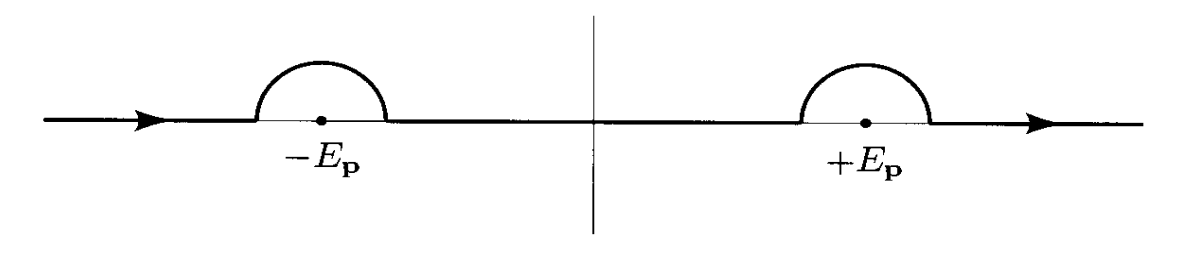
\includegraphics[scale=0.35]{QFT1/Green1.png}
\caption{Retarded Green Function}
\end{figure}

\[D_{\rm F}(x-y) \equiv \langle 0 | T\phi(x) \phi(y) | 0 \rangle = \int \frac{d^4 p}{(2\pi)^4} \frac{-i}{p^2+m^2-i\epsilon} e^{ip(x-y)},\]
where $T$ stands for time ordering, placing all operators evaluated at later times to the left.
\begin{figure}[!h]
\centering
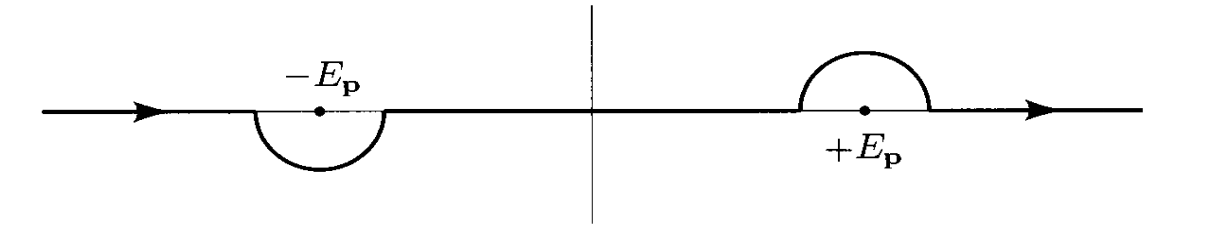
\includegraphics[scale=0.35]{QFT1/Green2.png}
\caption{Feynman Green Function}
\end{figure}

\section{Perturbation theory for canonical quantization}
\[\mathcal{L} = -\frac{1}{2}\partial_{\mu} \phi \partial^{\mu} \phi -\frac{1}{2}m_0^2 \phi^2 -\frac{\lambda_0}{4!}\phi^4.\]
\[H = H_0 + H_{\rm int} , \quad H_{\rm int} = \int d^3 x \frac{\lambda_0^4}{4!} \phi^4 (\bm{x}).\]

\subsection{Perturbation expansion of correlation functions}
\begin{note}
The ground state of the interaction field theory is denoted by $| \Omega \rangle$, the ground state of the free field theory is denoted by $| 0 \rangle$. The zero of energy is defined by $H_0 | 0 \rangle =0$ and $E_0 = \langle \Omega | H | \Omega \rangle$.
\end{note}
\noindent
Define
\[\phi(\bm{x}) \equiv \phi(t_0,\bm{x}) = \int \frac{d^3p}{(2\pi)^3}( a(\bm{p})e^{i\bm{p}\cdot\bm{x}} + a^{\dagger}(\bm{p})e^{-i\bm{p}\cdot\bm{x}}),\]
\[\phi(t,\bm{x}) = e^{iH(t-t_0)} \phi(\bm{x}) e^{-iH(t-t_0)},\]
\[\phi_{\rm I}(t,\bm{x}) \equiv e^{iH_0(t-t_0)} \phi(\bm{x}) e^{-iH_0(t-t_0)},\]
\[H_{\rm I}(x) \equiv \int d^3x \frac{\lambda_0^4}{4!} \phi_{\rm I}^4.\]
The perturbation expansion of correlation functions is
\[\langle \Omega | T \{ \phi(x) \phi(y) \} | \Omega \rangle = \lim_{T \to \infty(1-i\epsilon)} \frac{\langle 0 | T \left\{ \phi_{\rm I}(x) \phi_{\rm I}(y) \mathrm{exp} \left[ -i \int_{-T}^{T} dt H_{\rm I} \right]\right\} | 0 \rangle}{\langle 0 | T \left\{ \mathrm{exp} \left[ -i \int_{-T}^{T} dt H_{\rm I} \right]\right\} | 0 \rangle}.\]
The proof can be found in chapter 4.2 of \emph{An introduction to quantum field theory (M.E.Peskin \& D.V.Schroeder)}.
\\

\begin{newthem}[Wick's theorem]
\[T \left\{ \phi(x_1) \phi(x_2) \cdots \phi(x_n)\right\} = N \left\{ \phi(x_1) \phi(x_2) \cdots \phi(x_n) + \mbox{ all possible contractions }\right\} .\]
Normal order : all the $a$'s are to the right of all the $a^{\dagger}$.
\end{newthem}
\noindent
The proof can be found in chapter 4.3 of \emph{An introduction to quantum field theory (M.E.Peskin \& D.V.Schroeder)}.
\begin{example}
\begin{eqnarray}
\langle 0 | T \left\{ \phi_{\rm I}(x_1) \phi_{\rm I}(x_2) \phi_{\rm I}(x_3) \phi_{\rm I}(x_4)\right\}| 0 \rangle &=& D_{\rm F}(x_1-x_2)D_{\rm F}(x_3-x_4) \nonumber \\
&+& D_{\rm F}(x_1-x_3)D_{\rm F}(x_2-x_4) \nonumber \\
&+& D_{\rm F}(x_1-x_4)D_{\rm F}(x_2-x_3) .\nonumber
\end{eqnarray}
\end{example}

\subsection{Feynman diagram}
Expand $\langle 0 | T \left\{ \phi_{\rm I}(x) \phi_{\rm I}(y) \mathrm{exp} \left[ -i \int_{-T}^{T} dt H_{\rm I} \right]\right\} | 0 \rangle$ to the first order of $\lambda_0$. We have
\begin{eqnarray}
& &\langle 0 | T \left\{ \phi_{\rm I}(x) \phi_{\rm I}(y) \frac{-i\lambda_0}{4!} \int dz^4 \phi_{\rm I}(z) \phi_{\rm I}(z) \phi_{\rm I}(z) \phi_{\rm I}(z) \right\} | 0 \rangle \nonumber \\
&=& 3 \cdot (\frac{-i\lambda_0}{4!}) D_{\rm F}(x-y) \int d^4 z D_{\rm F}(z-z) D_{\rm F}(z-z) \nonumber \\
&+& 12 \cdot (\frac{-i\lambda_0}{4!}) \int d^4 z  D_{\rm F}(x-z) D_{\rm F}(y-z) D_{\rm F}(z-z) .\nonumber
\end{eqnarray}
It can be represented by the so called Feynman diagram.
\begin{figure}[!h]
\centering
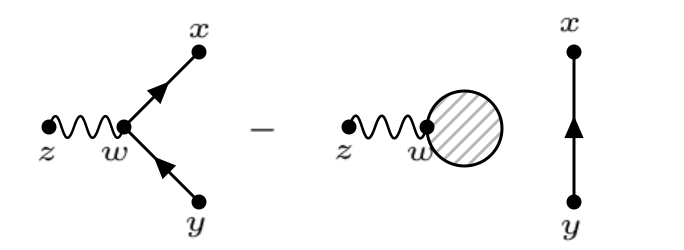
\includegraphics[scale=0.35]{QFT1/FD1.png}
\caption{Feynman diagram representation of perturbation expansion. The symmetry factor of the first diagram is $S = 4!/3 = 8$. The symmetry factor of the second diagram is $S = 4!/12 = 2$.}
\end{figure}
\noindent
The Feynman rules for $\phi^4$ theory are:
\begin{enumerate}
\item For each propagator, $P = D_{\rm F}(x-y)$
\item For each vertex, $V = (-i\lambda_0)\int d^4z$
\item For each external point, $E=1$
\item Divided by the symmetry factor
\end{enumerate}
At last, we can prove that
\[\langle \Omega | T \{ \phi_{\rm I}(x_1) \phi_{\rm I}(x_2) \cdots \phi_{\rm I}(x_n) \} | \Omega \rangle = \mbox{ sum of all E-connected diagrams with n external points},\]
where the ``E-disconnected'' means disconnected from all external points, being called ``vacuum bubbles''. They vacuum bubbles in $\langle 0 | T \left\{ \phi_{\rm I}(x_1) \phi_{\rm I}(x_2) \cdots \phi_{\rm I}(x_n) \mathrm{exp} \left[ -i \int_{-T}^{T} dt H_{\rm I} \right]\right\} | 0 \rangle$ are all cancelled by the $\langle 0 | T \left\{ \mathrm{exp} \left[ -i \int_{-T}^{T} dt H_{\rm I} \right]\right\} | 0 \rangle$.

\section{Path integral formulation}
\subsection{Basic formulation}
\noindent
Recall the path integrals formulation in quantum mechanics, we have
\[\langle \phi_b(\bm{x}) | e^{-iHT} | \phi_a(\bm{x}) \rangle = \int \mathcal{D}\phi \mathcal{D}\pi  \mathrm{exp} \left[ i\int_0^T d^4x (\pi\dot{\phi} - \frac{1}{2}\pi^2 - \frac{1}{2}(\nabla \phi)^2 -V(\phi))\right],\]
where $\langle \phi_b(\bm{x}) |$ is the eigenstate of $\phi_{\rm S}(\bm{x})=\phi_{\rm H}(\bm{x},0)$ with eigenvalue $\phi_b(\bm{x})$ at time $t=T$, $| \phi_a(\bm{x}) \rangle$ is the eigenstate of $\phi_{\rm S}(\bm{x})$ with eigenvalue $\phi_a(\bm{x})$ at time $t=0$.
Since the exponential is quadratic in $\pi$, we can complete the square and evaluate the $\mathcal{D}(\pi)$ integral to obtain
\[\langle \phi_b(\bm{x}) | e^{-iHT} | \phi_a(\bm{x}) \rangle = \int \mathcal{D}\phi  \mathrm{exp} \left[ i\int_0^T d^4x \mathcal{L} \right].\]
Now we can abandon the Hamiltonian formalism and take the the equation above to define the Hamiltonian dynamics.
\begin{note}
We emphasize that in this section, $\phi_{\rm H}$ denotes the Heisenberg picture of field whose value is operators,$\phi_{\rm S}$ denotes the Schr\"{o}dinger picture of field, $\phi(x)$ is classical field whose value is ordinary number.
\end{note}

\subsubsection{Correlation function}
\[\langle \Omega | T \phi_{\rm H}(x_1) \phi_{\rm H}(x_2)| \Omega \rangle = \lim_{T \to \infty(1-i\epsilon)} \frac{\int \mathcal{D}\phi \phi(x_1)\phi(x_2) \mathrm{exp} \left[ i\int_T^T d^4x \mathcal{L} \right]}{\int \mathcal{D} \phi \mathrm{exp} \left[ i\int_T^T d^4x \mathcal{L} \right]}.\]
The proof can be found in chapter 9.2 of \emph{An introduction to quantum field theory (M.E.Peskin \& D.V.Schroeder)}.

\subsubsection{Functional derivatives and the generating functional}
\noindent
We define the generating functional as
\[Z[J] \equiv \int \mathcal{D} \phi \mathrm{exp} \left[ i\int d^4x \mathcal{L} + J(x)\phi(x) \right].\]
We can prove that
\[\langle \Omega | T \phi_{\rm H}(x_1) \cdots \phi_{\rm H}(x_n) | \Omega \rangle = \frac{1}{Z[0]} \left. \left( -i\frac{\delta}{\delta J(x_1)} \right)\cdots \left( -i\frac{\delta}{\delta J(x_n)} \right) Z[J]\right|_{J=0},\]
where $Z[0] \equiv Z[J=0]$.

\subsection{Free field theory}
\noindent
In Klein-Gordon field theory,
\[\int d^4x [\mathcal{L}_0(\phi)+J\phi] = \int d^4x [\frac{1}{2}\phi (\partial^2 -m^2+i\epsilon)\phi + J\phi].\]
Define
\[\phi'(x) \equiv \phi(x) + \int d^4y (-iD_{\rm F}(x-y)) J(y) .\]
Recall that $(\partial^2-m^2)D_{\rm F}(x-y) = i\delta(x-y)$, we can derive that
\[\int d^4x [\mathcal{L}_0+J\phi] = \int d^4x [\frac{1}{2}\phi' (\partial^2 -m^2+i\epsilon)\phi'] - \int d^4x d^4y \frac{1}{2} J(x)[-iD_{\rm F}(x-y)]J(y).\]
After integration, we can know that
\[Z[J] = Z[0] \mathrm{exp} [-\frac{1}{2} \int d^4x d^4y J(x)D_{\rm F}(x-y)J(y)].\]
Thus
\[\langle 0 | T \phi_{\rm H}(x_1) \phi_{\rm H}(x_2) | 0 \rangle =  \frac{1}{Z[0]}- \frac{\delta}{\delta J(x_1)} \frac{\delta}{\delta J(x_2)} \mathrm{exp} \left. \left[-\frac{1}{2} \int d^4x d^4y JD_{\rm F}J\right] \right |_{J=0} = D_{\rm F}(x_1-x_2).\]

\subsection{Perturbation theory for path integral quantization}
The Lagrangian and generating functional of the $\phi^4$ theory is
\begin{eqnarray}
\mathcal{L} &=& -\frac{1}{2}\partial_{\mu} \phi \partial^{\mu} \phi -\frac{1}{2}m_0^2 \phi^2 -\frac{\lambda_0}{4!}\phi^4 .\nonumber \\
\mathcal{L} &=& \mathcal{L}_0 + \mathcal{L}_1 , \quad \mathcal{L}_1 =- \frac{\lambda_0}{4!} \phi^4 (\bm{x}). \nonumber \\
Z[J] &=& \int \mathcal{D}\phi e^{i\int d^4x [\mathcal{L}_0 + \mathcal{L}_1 + J\phi]} \nonumber \\
&=& e^{i\int d^4y \mathcal{L}_1(\frac{1}{i} \frac{\delta}{\delta J(y)})} \int \mathcal{D}\phi e^{i\int d^4x [\mathcal{L}_0 + J\phi]} \nonumber \\
& = & Z_0[0]e^{i\int d^4x \mathcal{L}_1(\frac{1}{i} \frac{\delta}{\delta J(x)})} \mathrm{exp} \left[-\frac{1}{2} \int d^4y d^4z J(y)D_{\rm F}(y-z)J(z)\right] \nonumber \\
& =& Z_0[0]\sum_{V=0}^{\infty} \frac{1}{V!} \left[ \frac{-i\lambda_0}{4!} \int d^4x \left(\frac{1}{i} \frac{\delta}{\delta J(x)}\right)^4\right]^V \times \sum_{P=0}^{\infty} \frac{1}{P!} \left[-\frac{1}{2} \int d^4y d^4z J(y)D_{\rm F}(y-z)J(z)\right]^P .\nonumber
\end{eqnarray}
If we focus on a term with particular values of $V$ and $P$, then the number of surviving sources (after we take all the functional derivatives) is $E = 2P-4V$. The $4V$ functional derivatives can act on the 2P sources in ${(2P)!}/{(2P-4V)!}$ different combinations. However, many of the resulting expressions are algebraically identical.
\\ \\
To organize them, we introduce Feynman diagrams similar to that in perturbation theory of canonical quantization. In these diagrams, a line segment stands for a propagator $D_{\rm F}(x-y)$, a filled circle at one end of a line segment for a source $i\int d^4x J(x)$, and a vertex joining four line segments for $-i\lambda_0 \int d^4 z$.
\\ \\
For each diagram, we can assign a symmetry factor $S_P$ similar to that in perturbation theory for canonical quantization. Due to the fact that some external sources are identical here, usually $S_P \neq S_C$. But when calculating the correlation function, the exchange of the order of functional derivatives to identical sources can eliminate the difference.
\\ \\
We can demonstrate that
\[Z[J] = Z_0[0] \mathrm{exp}(\sum_I C_I),\]
where $C_I$ stands for a particular connected diagram, including its symmetry factor. We can define $W[J]$ as
\[Z[J] \equiv Z[0] \mathrm{exp}(-iW[J]).\]
As $W[0]=0$, we know
\[-iW[J] = \sum_{I \neq \{0\}} C_I.\]
The notation $I\neq \{0\}$ means that the vacuum diagrams are omitted from the sum.
The detailed discussion can be found in chapter 9 of \emph{Quantum field theory (M. Srednicki)}.

\subsection{Symmetries in the functional formalism}
\subsubsection{Equations of motion}
\noindent
The correlation function of the field theory is given by
\[\langle \Omega | T \phi_{\rm H}(x_1) \cdots \phi_{\rm H}(x_n) | \Omega \rangle = Z[0]^{-1} \int \mathcal{D}\phi e^{iS} \phi(x_1)\cdots\phi(x_n).\]
The equation of motion of classical field theory will be give by
\[\frac{\delta S}{\delta \phi(x)} = 0.\]
In quantum field theory, we derive the equation of motion by claim that the path integral will be invariant under the infinitesimal change of field, i.e. $\phi(x) \to \phi(x) + \epsilon(x)$.
Define
\[Z[\phi(x_1),\cdots,\phi(x_n)] \equiv  \int \mathcal{D}\phi e^{iS} \phi(x_1)\cdots\phi(x_n).\]
We know
\[\delta Z = \int \mathcal{D}\phi e^{iS} \left\{ \int d^4x \epsilon(x) \left[ i\frac{\delta S}{\delta \phi(x)} \phi(x_1)\cdots\phi(x_n) + \delta(x-x_1)\cdots\phi(x_n) + \cdots + \phi(x_1)\cdots\delta(x-x_n) \right]\right\} .\]
Thus
\[\langle \frac{\delta S}{\delta \phi(x)} \phi(x_1)\cdots\phi(x_n) \rangle  = \sum_{i=1}^{n} \langle \phi(x_1) \cdots (i\delta(x-x_i)) \cdots \phi(x_n) \rangle.\]
\begin{example}
For Klein-Gordon field,
\[\mathcal{L} = -\frac{1}{2}\phi^{\mu}\phi \partial_{\mu}\phi - \frac{1}{2}m^2\phi^2.\]
The variation of $S$ gives
\[\frac{\delta S}{\delta \phi(x)} = (\partial^2-m^2)\phi(x).\]
Thus we can get
\[(\partial^2-m^2) \langle 0 | T \phi(x)\phi(x_1)| 0 \rangle = i\delta(x-x_1).\]
\end{example}

\subsubsection{Conservation law}
Consider a local field theory of a set of fields $\phi_a(x)$, governed by a Lagrangian $\mathcal{L}(\phi)$. An infinitesimal symmetry transformation on the fields $\phi_a$ will be of the general form 
\[\phi_a(x) \to \phi_a(x) + \epsilon \Delta \phi_a(x).\]
We assume that when $\epsilon$ is a constant, the action is invariant under this transformation. Then the Lagrangian must be invariant up to a total divergence:
\[\mathcal{L}[\phi] \to \mathcal{L}[\phi] + \epsilon \partial_{\mu} K^{\mu}.\]
If the symmetry parameter $\epsilon$ depend on $x$, the variation of Lagrangian will be
\[L[\phi] \to \mathcal{L}[\phi] + (\partial_{\mu}\epsilon)\Delta \phi_a \frac{\partial \mathcal{L}}{\partial (\partial_{\mu}\phi_a)} + \epsilon \partial_{\mu} K^{\mu}.\]
Thus
\[\frac{\delta S}{\delta \epsilon(x)} = \partial_{\mu} j^{\mu} , \quad j^{\mu} = -\frac{\partial \mathcal{L}}{\partial (\partial_{\mu}\phi_a)}\Delta \phi_a + K^{\mu} .\]
If the measure $\mathcal{D}\phi$ is invariant under the transformation, we can derive similarly that
\[\langle \partial_{\mu} j^{\mu}(x) \phi(x_1)\cdots\phi(x_n) \rangle  = \sum_{i=1}^{n} \langle \phi(x_1) \cdots (i\Delta \phi(x_i)\delta(x-x_i)) \cdots \phi(x_n) \rangle.\]

\section{Cross section and the S-matrix}
\noindent
For a relativistic collinear scattering process, we have
\[dN = \sigma |\bm{v}_1 - \bm{v}_2| n_1 dt.\]
Consider a  $2 \to n$ process:
\[p_1 + p_2 \to \{p_j\}.\]
Suppose the volume of the space in which the scattering process takes place is $V$, the duration of the scattering process is $T$. 
Therefore, the density of incident particle is
\[n_1 = \frac{1}{V}\]
and the number of events is
\[N = \frac{|\langle i | S | f \rangle|^2}{|\langle i | i \rangle||\langle f | f \rangle|} d\Pi ,\]
where $d\Pi$ is the region of final state momenta at which we are looking
\[d\Pi = \prod_j \frac{V}{(2\pi)^3} d^3 p_j.\]
Recall that
\[\delta^{(3)}(0) = \frac{V}{(2\pi)^3} , \quad \delta^{(4)}(0) = \frac{VT}{(2\pi)^4} , \quad \langle p | p \rangle = (2\pi)^3 2\omega \delta^{(3)}(0).\]
Write the scattering amplitude in the form of
\[\langle i | S | f \rangle = i\mathcal{M}(2\pi)^4\delta(\sum p_f-\sum p_i).\]
We can get that
\[|\langle i | S | f \rangle|^2 = |\mathcal{M}|^2 VT (2\pi)^4 \delta(\sum p_j - p_1 - p_2) , \quad \langle i | i \rangle = (2E_1V) (2E_2V) , \quad \langle f | f \rangle = \prod_j (2E_jV).\]
At last, putting everything together, we have
\[d\sigma = \frac{1}{(2E_1)(2E_2)|\bm{v}_1-\bm{v}_2|} |\mathcal{M}|^2 d\Pi_{\mathrm{LIPS}},\]
where
\[d\Pi_{\mathrm{LIPS}} = \prod_j \frac{d^3p_j}{(2\pi)^3} \frac{1}{2E_j} (2\pi)^4 \delta(\sum p_j - p_1 - p_2)\]
is called the Lorentz-invariant phase space (LIPS).
All the factors of $V$ and $T$ have dropped out, so now it is trivial to take $V \to \infty$ and $T \to \infty$. 

\subsubsection{Decay rates}
\noindent
The definition of decay rates is
\[\Gamma \equiv \frac{\mbox{Number of Events}}{\mbox{Time}}.\]
Consider a  $1 \to n$ process:
\[p_1 \to \{p_j\}.\]
We can derive the decay rates by the similar method,
\[d\Gamma = \frac{1}{2E_1} |\mathcal{M}|^2 d\Pi_{\mathrm{LIPS}} .\]

\subsubsection{Special cases}
\noindent
For $2 \to 2$ scattering in the center-of-mass frame
$p_1 + p_2 \to p_3 + p_4$,
the LIPS is
\[d\Pi_{\mathrm{LIPS}} = \frac{d^3p_3}{(2\pi)^3} \frac{1}{2E_3 } \frac{d^3p_4}{(2\pi)^3} \frac{1}{2E_4} (2\pi)^4 \delta(p_3+p_4-p_1-p_2).\]
We can now integrate over $\bm{p}_4$ to give
\[d\Pi_{\mathrm{LIPS}} = \frac{1}{16\pi^2} d\Omega \int dp_f \frac{p_f^2}{E_3 E_4} \delta(E_3+E_4 -E_{CM}),\]
where $p_f \equiv |\bm{p}_3| = |\bm{p}_4|$ and $E_{CM} \equiv E_1 + E_2$.
Define $x(p_f) \equiv E_3 + E_4 - E_{CM}$, we can get
$dx/dp_f = (E_3+E_4)p_f/E_3E_4$.
Thus
\[d\Pi_{\mathrm{LIPS}} = \frac{1}{16\pi^2} d\Omega \frac{p_f}{E_{CM}}\theta (E_{CM} - m_3 -m_4).\]
Plugging this into the general equation for cross section, we can get
\[ \frac{d\sigma}{d\Omega} = \frac{1}{64\pi^2 E_{CM}^2} \frac{|\bm{p}_f|}{|\bm{p}_i|} |\mathcal{M}|^2 \theta (E_{CM} - m_3 -m_4) .\]
If all the masses are equal then this formula simplifies further
\[\frac{d\sigma}{d\Omega} = \frac{1}{64\pi^2 E_{CM}^2} |\mathcal{M}|^2.\]

\section{LSZ reduction formula}
\subsection{Field strength renormalization}
\noindent
We have the completeness relation:
\[\bm{1} = |\Omega\rangle\langle\Omega| +  \sum_{\lambda} \int \frac{d^3p}{(2\pi)^3} \frac{1}{2E_{\bm{p}}} |\lambda_{\bm{p}}\rangle\langle\lambda_{\bm{p}}|,\]
where $E_{\bm{p}} \equiv \sqrt{m_{\lambda}^2 + \bm{p}^2}$.
\\
\begin{figure}[!h]
\centering
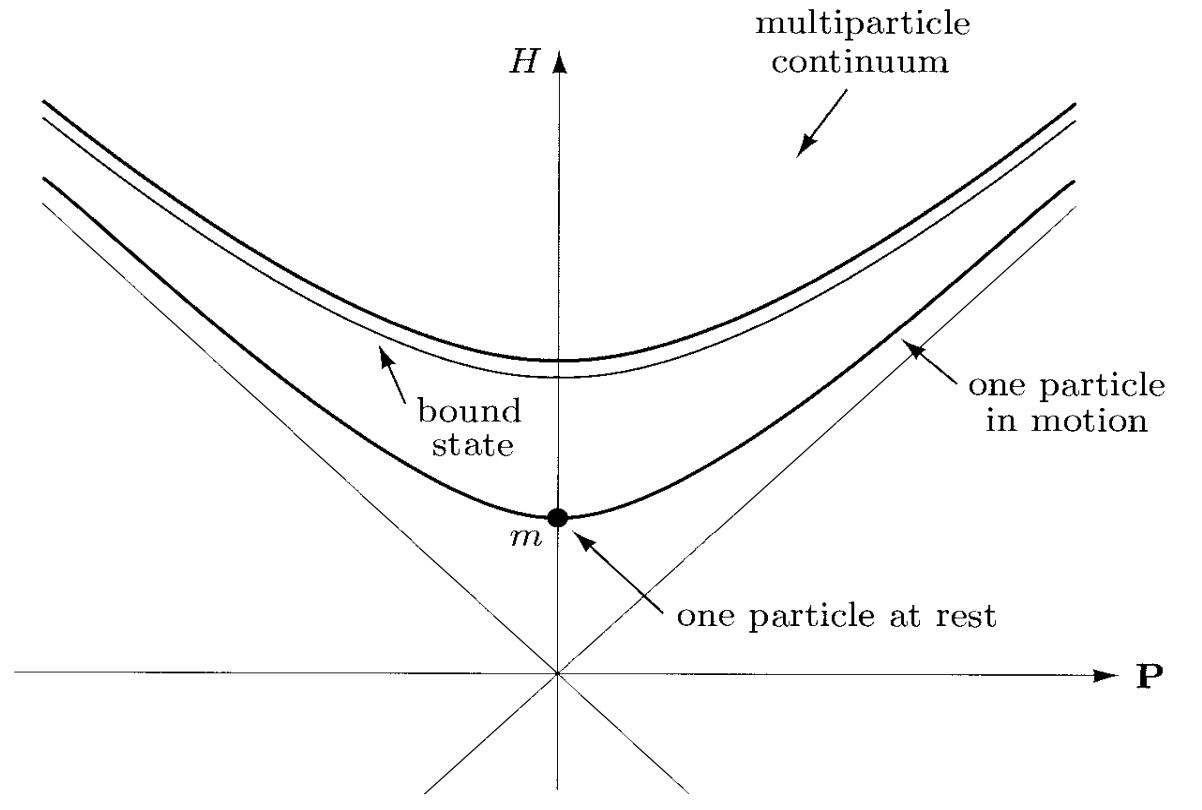
\includegraphics[scale = 0.3]{QFT1/FSR1.png}
\caption{Particle's energy-momentum relation}
\end{figure}
\\
Assume for now $x^0 > y^0$ and define $\langle \Omega | \phi(x) \phi(y) | \Omega \rangle_{C} = \langle \Omega | \phi(x) \phi(y) | \Omega \rangle - \langle \Omega | \phi(x)| \Omega \rangle \langle \Omega | \phi(y) | \Omega \rangle$ as connected two point function. (The term $\langle \Omega | \phi(x)| \Omega \rangle \langle | \Omega \phi(y) | \Omega \rangle$ is usually zero by symmetry; for higher spin fields, it is zero by Lorentz invariance.) The connected two point function is
\[\langle \Omega | \phi(x) \phi(y) | \Omega \rangle_{C} = \sum_{\lambda} \int \frac{d^3p}{(2\pi)^3} \frac{1}{2E_{\bm{p}}} \langle \Omega | \phi(x) |\lambda_{\bm{p}}\rangle\langle\lambda_{\bm{p}}| \phi(y) | \Omega \rangle.\]
It can be verified that
\[\langle \Omega | \phi(x) |\lambda_{\bm{p}}\rangle = \langle \Omega | \phi(0) | \lambda_0 \rangle e^{ipx} |_{p^0 = E_{\bm{p}}}.\]
Thus
\[\langle \Omega | \phi(x) \phi(y) | \Omega \rangle_C = \sum_{\lambda} \int \frac{d^4p}{(2\pi)^4} \frac{-i}{p^2 + m_{\lambda}^2 -i\epsilon} e^{ip(x-y)} |\langle \Omega | \phi(0) | \lambda_0 \rangle|^2.\]
Analogous expressions hold for the case $y^0 > x^0$, and both cases can be summarized as
\[\langle \Omega | T \phi(x) \phi(y) | \Omega \rangle_C = \int_0^{\infty} \frac{dM^2}{2\pi} \rho(M^2) D_{\rm F}(x-y;M^2),\]
where 
\[\rho(M^2) \equiv \sum_{\lambda} (2\pi) \delta(M^2-m_{\lambda}^2)|\langle \Omega | \phi(0) | \lambda_0 \rangle|^2 .\]
\begin{figure}[!h]
\centering
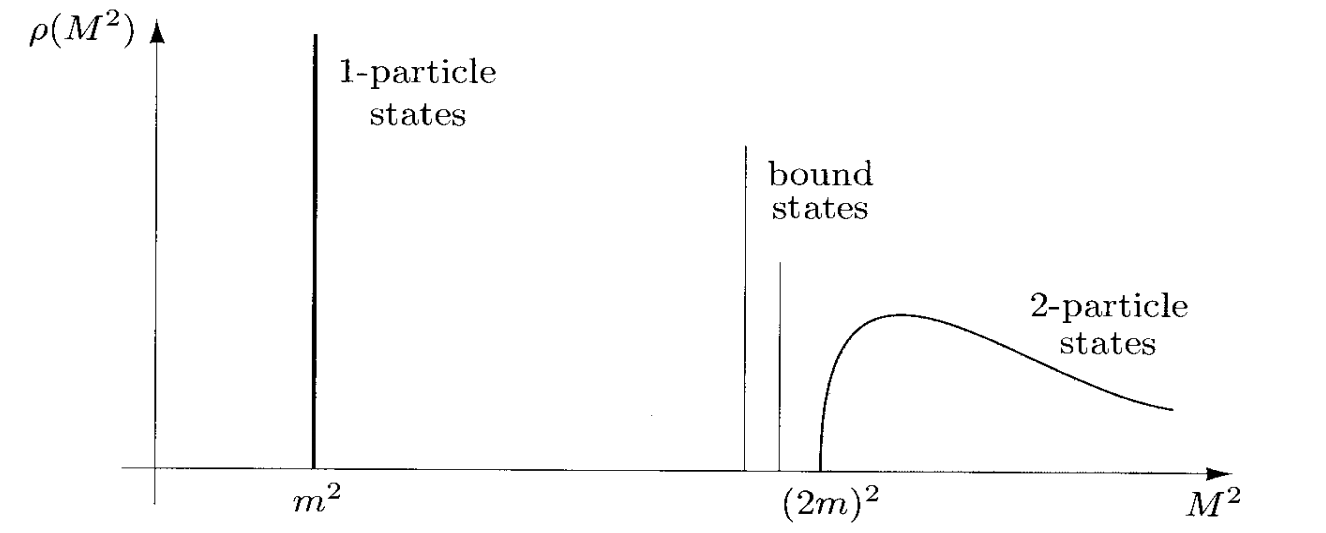
\includegraphics[scale=0.3]{QFT1/FSR2.png}
\caption{The structure of the spectral density function $\rho(M^2)$}
\end{figure}
\\
The one-particle state contribute an isolated delta function to the spectral density function, so
\[\rho(M^2) = 2\pi \delta (M^2 -m^2) \cdot Z + \mbox{ (nothing else until $M^2 > \sim (2m)^2$) }.\]
$Z = |\langle \Omega | \phi(0) | \lambda_0 \rangle|^2$ is called field-strength renormalization. $m$ is the physical mass of a single particle of the $\phi$ boson. The Fourier transformation of the two point function is
\begin{eqnarray}
&\phantom{=}& \int d^4x e^{-ipx} \langle \Omega | T \phi(x) \phi(0) | \Omega \rangle_C \nonumber \\  
&=& \int_{0}^{\infty} \frac{dM^2}{2\pi} \rho(M^2) \frac{-i}{p^2+M^2-i\epsilon} = \frac{-iZ}{p^2+m^2-i\epsilon} +  \int_{\sim 4m^2}^{\infty} \frac{dM^2}{2\pi} \rho(M^2) \frac{-i}{p^2+M^2-i\epsilon} .\nonumber
\end{eqnarray}
\begin{figure}[!h]
\centering
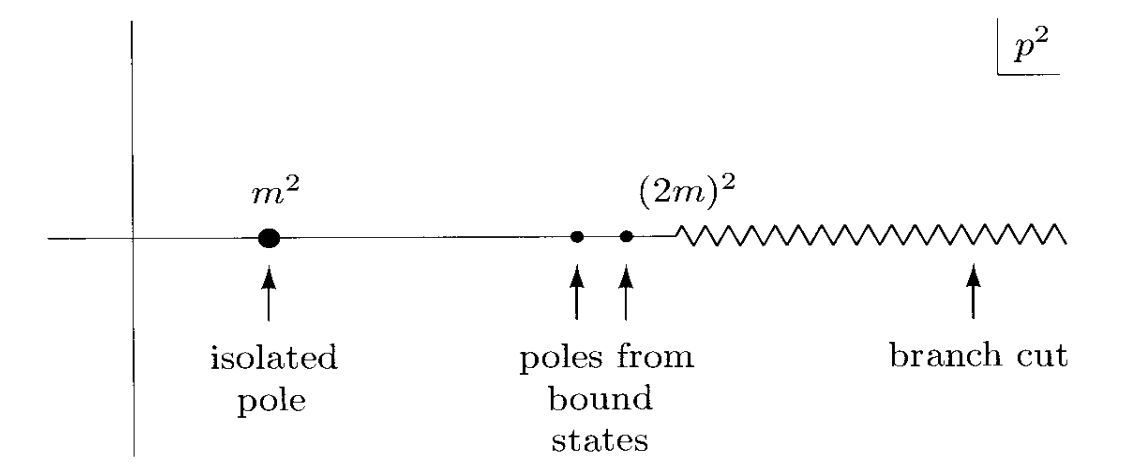
\includegraphics[scale=0.3]{QFT1/FSR3.png}
\caption{The structure of the two point function in Fourier space}
\end{figure}
\vspace{80pt}

\subsection{LSZ reduction formula}
\begin{newthem}[LSZ reduction formula]
\begin{eqnarray}
&& \quad \prod_1^n \int d^4 x_i e^{-ip_ix_i} \prod_1^m d^4 y_j e^{ik_jy_j} \langle \Omega | T \{\phi(x_1) \cdots \phi(x_n) \phi(y_1) \cdots \phi(y_m)\} | \Omega \rangle \nonumber \\
&& \underset{ p_i^0 \to E_{\bm{p}_i}\, k_i^0 \to E_{\bm{k}_i}}{\sim}  \left( \prod_1^n \frac{-\sqrt{Z} i}{p_i^2 + m^2 -i\epsilon} \right) \left( \prod_1^m \frac{-\sqrt{Z} i}{k_i^2 + m^2 -i\epsilon} \right) \langle \bm{p}_1 \cdots \bm{p}_n | S | \bm{k}_1 \cdots \bm{k}_m \rangle .\nonumber
\end{eqnarray}
\end{newthem}
\noindent
The $\sim$ means the two sides of the expression share the same singular structure around $p_i^0 \to E_{\bm{p}_i}$, $k_i^0 \to E_{\bm{k}_i}$.
The proof can be found in chapter 7.2 of \emph{An introduction to quantum field theory (M.E.Peskin \& D.V.Schroeder)}.
To express the formula above in the language of Feynman diagrams, we consider the S-matrix element for 2-particle $\to$ 2-particle for example. Note the disconnected diagram should be disregarded because they do not have the singularity structure with a product of four poles indicated by on the right side of the LSZ reduction formula. Thus the exact four point function
\[\prod_1^2 \int d^4 x_i e^{-ip_ix_i} \prod_1^2 d^4 y_i e^{ik_jy_j} \langle \Omega | T \{\phi(x_1)\phi(x_2)\phi(y_1) \phi(y_2)\} | \Omega \rangle \]
can be represented by amputated Feynman diagram.
\begin{figure}[!h]
\centering
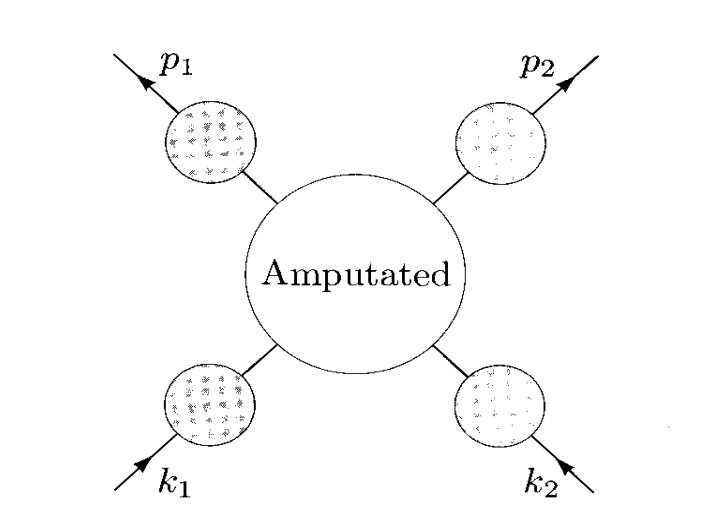
\includegraphics[scale=0.3]{QFT1/LSZ1.png}
\caption{Amputated Feynman diagram}
\end{figure}
\\
We can sum up the corrections to each external leg. Let $-iM^2(p^2)$ denote the sum of all 1PI insertions into the scalar propagator.
\begin{figure}[!h]
\centering
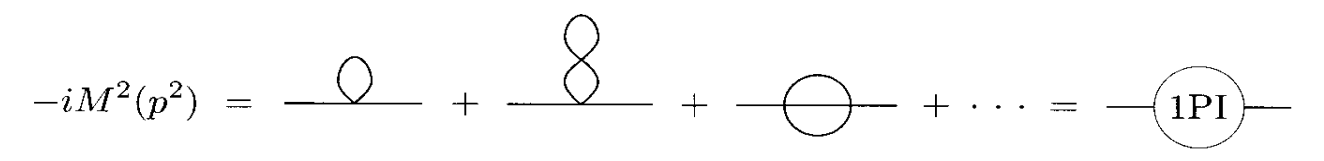
\includegraphics[scale=0.25]{QFT1/LSZ2.png}
\caption{Diagram representation of 1PI propagator}
\end{figure}
\begin{note}
One-particle-irreducible, or 1PI for short, refers to diagrams that is still connected after one line is cut
\end{note}
\noindent
Then the exact propagator can be written as a geometric series of 1PI propagators.
\begin{figure}[!h]
\centering
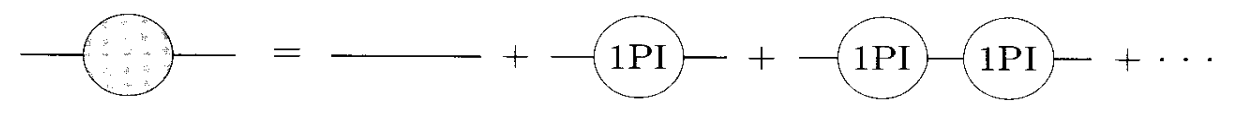
\includegraphics[scale=0.25]{QFT1/LSZ3.png}
\caption{Diagram representation of exact propagator}
\end{figure}
\\
The result is ${-i}/{(p^2 + m_0^2 + M^2)}$. If we expand each resummed propagator about the physical particle pole, we see that each external leg of the four-point amplitude contributes
\[\frac{-i}{p^2 + m_0^2 + M^2} \underset{p^0 \to E_{\bm{p}}}{\sim} \frac{-iZ}{p^2+m^2} + \mbox{ (regular) }.\]
Thus, the sum of diagrams contains a product of four point poles:
\[\frac{-iZ}{p_1^2 + m^2} \frac{-iZ}{p_2^2 + m^2} \frac{-iZ}{k_1^2 + m^2} \frac{-iZ}{k_2^2 + m^2}.\]
Thus the S matrix element can be represented by the following diagram.
\begin{figure}[!h]
\centering
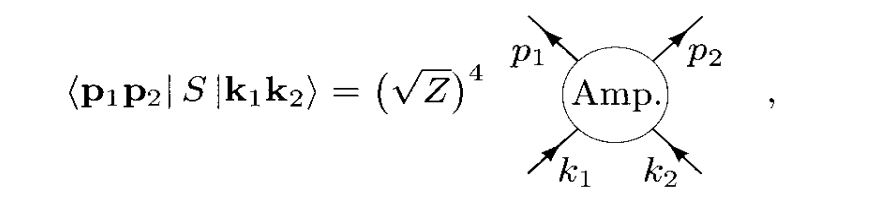
\includegraphics[scale=0.3]{QFT1/LSZ4.png}
\caption{Feynman diagram representation of LSZ reduction formula}
\end{figure}
\\
It is easy to be generalized to the more complicated scattering cases. After Fourier transforming the n-point function to momentum space and cutting off the external legs, the Feynman rules for S-matrix element can be stated as follows:
\begin{enumerate}
\item For each propagator, $P = {-i}/{(p^2 + m_0^2 -i\epsilon)}$;
\item For each vertex, $V = -i\lambda_0$;
\item For each external point, $E=1$;
\item Impose momentum conservation at each vertex;
\item Integrate over each undetermined loop momentum: $\int {d^4p}/{(2\pi)^4}$;
\item Divided by the symmetry factor;
\item Multiply the total momentum conservation factor $(2\pi)^4 \delta(\sum p_f - \sum p_i)$ .
\end{enumerate}
We can write $\langle f | S | i \rangle = (Z_1)^{\frac{n_s}{2}} i \mathcal{M} (2\pi)^4 \delta(\sum p_f - \sum p_i)$ for convenience.

\section{Renormalization}
Renormalization, the procedure in quantum field theory by which divergent parts of a calculation, leading to nonsensical infinite results, are absorbed by redefinition into a few measurable quantities, so yielding finite answers.

\subsection{Counting of ultraviolet divergence}
Consider a pure scalar theory in $d$ dimensions with a $\phi^n$ interaction term
\[\mathcal{L} = -\frac{1}{2} \partial^{\mu} \phi \partial_{\mu} \phi -\frac{1}{2}m^2 \phi^2 - \frac{\lambda}{n!}\phi^n.\]
Let $N$ be the number of external lines in the diagram, $P$ the number of propagators, $V$ the number of vertices. The number of the loops in the diagram is $L=P-V+1$.  There are $n$ lines meeting at each vertex, so $nV = 2P+N$. Loosely speaking, each loop has an integral $d^d p$, each propagator has a factor $p^{-2}$, so the superficial degrees of divergence is
\[D = dL - 2P = d + [n(\frac{d-2}{2})-d)]V - (\frac{d-2}{2})N.\]
According the superficial degrees of divergence of the diagram. There are three possible types of ultraviolet behaviour of quantum field theories. We will refer to them as follows.

\begin{enumerate}
\item Super-renormalizable theory: Only a finite number of Feynman diagrams superficially diverge.
\item renormalizable theory: Only a finite number of amplitudes superficially diverge; however, divergences
occur at all orders in perturbation theory. 
\item Non-renormalizable theory: All amplitudes are divergent at a sufficiently high order in perturbation
theory.
\end{enumerate}
\noindent
Therefore, for $\phi^4$ theory in four dimension, $D = 4 - N$. It is a renormalizable theory. For $\phi^3$ theory in four dimension, $D = 4 - V -N$. It is a super-renormalizable theory. For $\phi^6$ theory in four dimension, $D = 4 + 2V -N$. It is a Non-renormalizable theory. 
\\ \\
The superficial degrees of freedom can also be derived from dimensional analysis. The dimension of $\lambda$ is $d - {n(d-2)}/{2}$. Now consider an arbitrary diagram with $N$ external lines. One way that such a diagram could arise is from an interaction term $\eta \phi^N$ in the Lagrangian. The dimension of $\eta$ would then be $d - {N(d-2)}/{2}$, and therefore we conclude that any (amputated) diagram with $N$ external lines has dimension $d - {N(d-2)}/{2}$. 
In our theory with only the $\lambda \phi^n$ vertex, if the diagram has $V$ vertices, its divergent part is proportional to $\lambda^V \Lambda^D$, where $\Lambda$ is a high momentum cut-off and $D$ is the superficial degree of divergence.  Applying dimensional analysis, we find
\[d - \frac{N(d-2)}{2} = V[d - \frac{n(d-2)}{2}] + D.\]
Note that the quantity that multiplies $V$ in this expression is just the dimension of the coupling constant $\lambda$. Thus we can characterize the three degrees of renormalizability in a second way:

\begin{enumerate}
\item Super-renormalizable: Coupling constant has positive mass dimension.
\item  renormalizable: Coupling constant is dimensionless.
\item  Non-renormalizable: Coupling constant has negative mass dimension.
\end{enumerate}

\subsection{Renormalized perturbation theory}
The Lagrangian of $\phi^4$ theory is 
\[\mathcal{L} = -\frac{1}{2} \partial^{\mu} \phi \partial_{\mu} \phi -\frac{1}{2}m_0^2 \phi^2 - \frac{\lambda_0}{4!}\phi^4.\]
\\
We write $m_0$ and $\lambda_0$, to emphasize that these are the bare values of the mass and coupling constant, not the values measured in experiments.
Since the theory is invariant under $\phi \to -\phi$, all amplitudes with an odd number of external legs vanish. The only divergent amplitudes are therefore
\begin{figure}[!h]
\centering
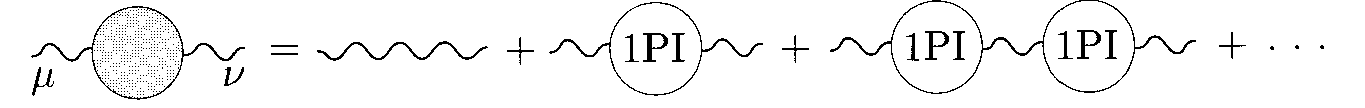
\includegraphics[scale=0.35]{QFT1/RG1.png}
\caption{Divergence of $\phi^4$ theory}
\end{figure}
\\
Ignoring the vacuum diagram, these amplitudes contain three infinite constants. Our goal is to absorb these constants into the three unobservable parameters of the theory: the bare mass, the bare coupling constant, and the field strength. To accomplish this goal, it is convenient to reformulate the perturbation expansion so that these unobservable quantities do not appear
explicitly in the Feynman rules. Recall that the exact two-point function has the form
\[\int d^4x \langle \Omega | \phi(x) \phi(0) | \Omega \rangle e^{-ipx} = \frac{-iZ}{p^2+m^2} + \mbox{ terms regular at } p^2 = m^2.\]
We can eliminate the $Z$ from this equation by rescaling the field:
$\phi = Z^{\frac{1}{2}} \phi_r$
We also define
\[\delta_Z = Z -1 , \quad \delta_m = Zm_0^2 - m^2 , \quad \delta_{\lambda} = \lambda_0 Z^2 - \lambda.\]
Then the Lagrangian becomes
\[\mathcal{L} = -\frac{1}{2} \partial^{\mu} \phi_r \partial_{\mu} \phi_r -\frac{1}{2}m^2 \phi_r^2 - \frac{\lambda}{4!}\phi_r^4 -\frac{1}{2} \delta_Z \partial^{\mu} \phi_r \partial_{\mu} \phi_r -\frac{1}{2}\delta_m \phi_r^2 - \frac{\delta \lambda}{4!}\phi_r^4.\]
The last three terms, known as counter-terms, have absorbed the infinite but unobservable shifts between the bare parameters and the physical parameters.We give precise definitions of the physical mass and coupling constant as renormalization conditions below.
\\
\begin{figure}[!h]
\centering
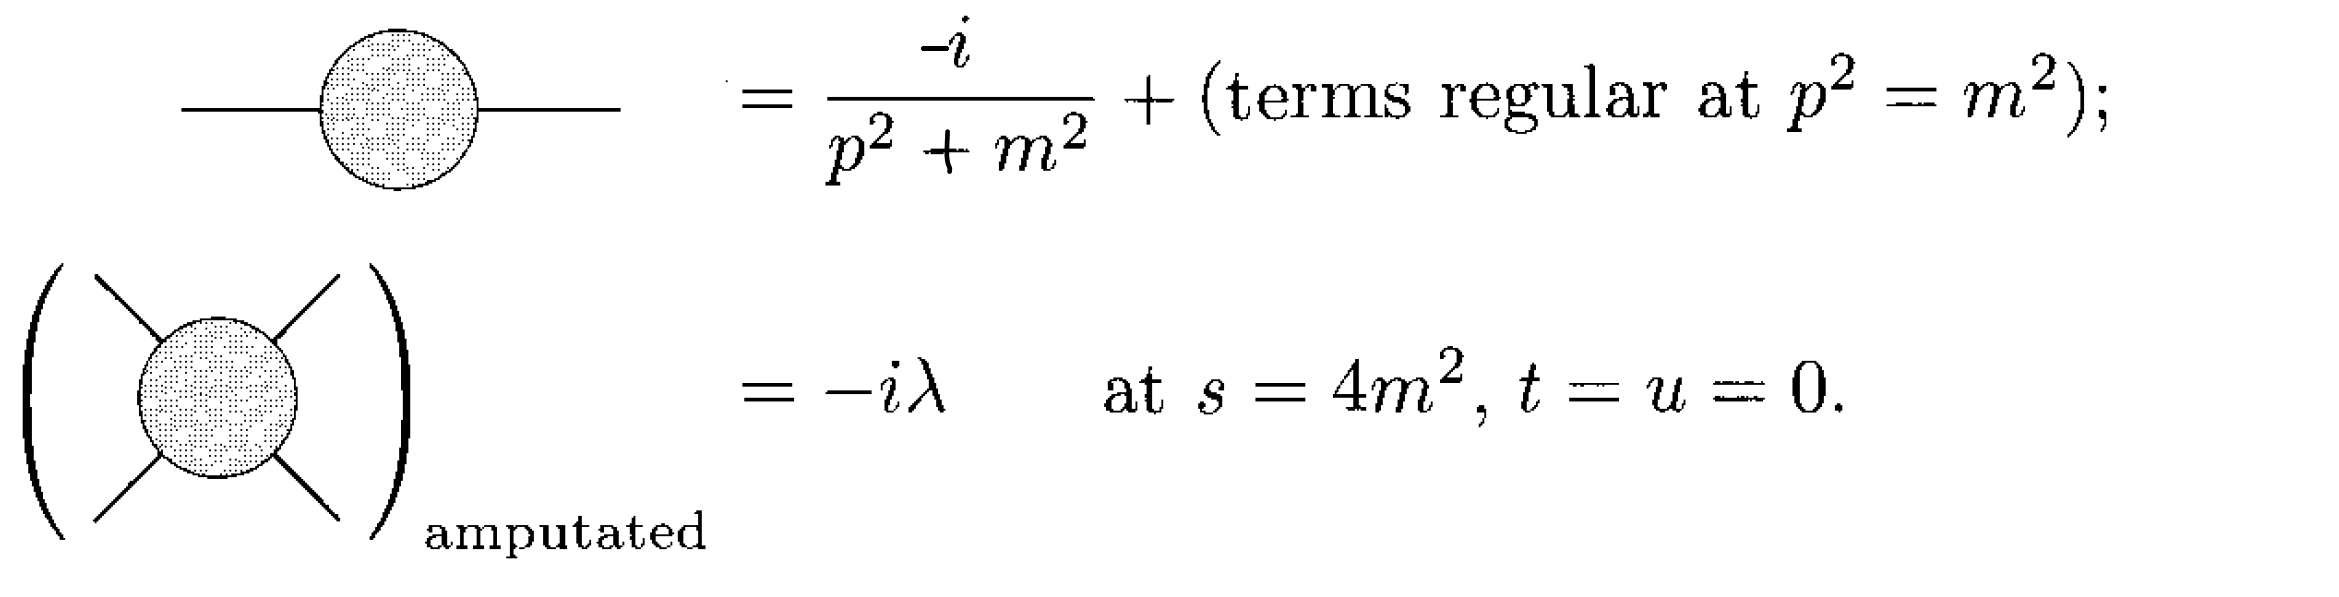
\includegraphics[scale=0.35]{QFT1/RG2.png}
\caption{On-shell (OS) renormalization conditions}
\end{figure}
\begin{figure}[!h]
\centering
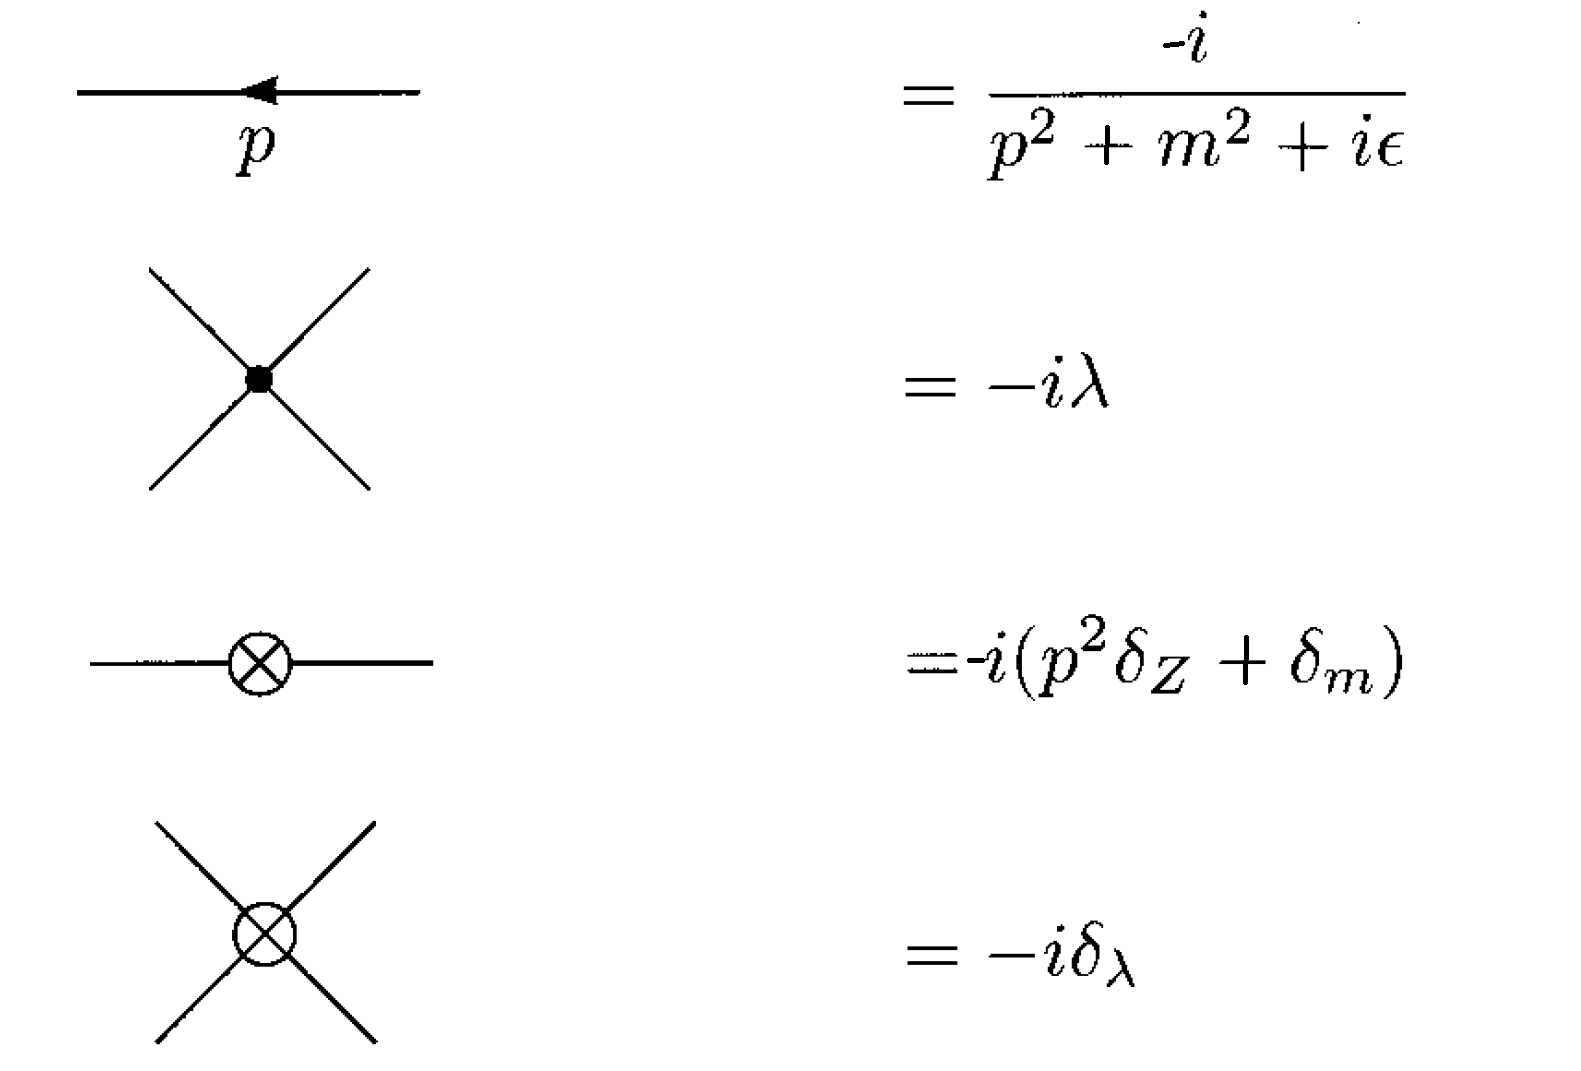
\includegraphics[scale=0.35]{QFT1/RG3.png}
\caption{Feynman rules for renormalized perturbation theory}
\end{figure}
\\
We can use Feynman rules to compute any amplitude in $\phi^4$ theory. The procedure is as follows. Compute the desired amplitude as the sum of all possible diagrams created from the propagator and vertices shown above. The loop integrals in the diagrams will often diverge, so one must introduce a regulator. The result of this computation will be a function of the three unknown parameters $\delta_Z$, $\delta_m$, and $\delta_{\lambda}$. Adjust ( or ``renormalise'') these three parameters as necessary to maintain the renormalization conditions. After this adjustment, the expression for the amplitude should be finite and independent of the regulator.
This procedure, using Feynman rules with counter-terms, is known as renormalized perturbation theory. 

\subsubsection{Mandelstam variable}
In theoretical physics, the \href{https://en.wikipedia.org/wiki/Mandelstam_variables}{\textbf{Mandelstam variable}}  are numerical quantities that encode the energy, momentum, and angles of particles in a scattering process in a Lorentz-invariant fashion. They are used for scattering processes of two particles to two particles. 
The Mandelstam variables $s$, $t$, $u$ are then defined by
\begin{eqnarray}
s=-(p_{1}+p_{2})^{2}=-(p_{3}+p_{4})^{2} ,\nonumber \\
t=-(p_{1}-p_{3})^{2}=-(p_{2}-p_{4})^{2} ,\nonumber \\
u=-(p_{1}-p_{4})^{2}=-(p_{2}-p_{3})^{2} ,\nonumber
\end{eqnarray}
where $p_1$ and $p_2$ are the four-momenta of the incoming particles and $p_3$ and $p_4$ are the four-momenta of the outgoing particles.
$s$ is also known as the square of the center-of-mass energy (invariant mass) and $t$ is also known as the square of the four-momentum transfer.
We can verify that
\[s+t+u = m_1^2 + m_3^2 + m_3^2 +m_4^2.\]

\subsection{Techniques for renormalization}
\subsubsection{Feynman's formula}
\begin{newthem}[Feynman's formula]
\[ \frac{1}{A_1 \cdots A_n} = \int dF_n (x_1A_1+ \cdots +x_nA_n)^{-n},\]
where the integration measure over the Feynman parameters $x_i$ is
\[\int dF_n = (n-1)! \int_0^1 dx_1 \cdots dx_n \delta(x_1+\cdots+x_n-1).\]
This measure is normalized so that
\[\int dF_n = 1.\]
A generalization of Feynman's formula is
\[ \frac{1}{A_1^{\alpha_1} \cdots A_n^{\alpha_n}} = \frac{\Gamma(\sum_i \alpha_i)}{\prod_i \Gamma(\alpha_i)} \frac{1}{(n-1)!}\int dF_n \frac{\prod_i x_i^{\alpha_i-1}}{(\sum_i x_i A_i)^{\sum_i \alpha_i}}.\]
\end{newthem}
\begin{figure}[!h]
\centering
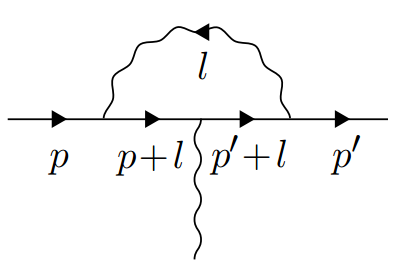
\includegraphics[scale=0.35]{QFT1/RG5.png}
\caption{Wick rotation}
\end{figure}

\subsubsection{Wick rotation}
For an integral $\int d^d q f(q^2-i\epsilon)$, if the integrand vanishes fast enough as $|q_0| \to \infty$, we can rotate this contour clockwise by ${\pi}/{2}$, so that it runs from $-i\infty$ to $i\infty$. In making this Wick rotation, the contour does not pass over any poles. (The $i\epsilon$ are needed to make this statement unambiguous.) Thus the value of the integral is unchanged. It is now convenient to define a Euclidean $d$-dimensional vector $\bar{q}$ via $q^0 = i \bar{q}_d$ and $q_j = \bar{q}_j$; then $q^2 = \bar{q}^2$, where
\[\bar{q}^2 = \bar{q}_1^2 + \cdots + \bar{q}_d^2.\]
Also, $d^dq = id^d \bar{q}$. Therefore, in general,
\[\int d^d q f(q^2-i\epsilon) = i \int d^d\bar{q} f(\bar{q}^2).\]

\subsubsection{Dimensional regularization}
Dimensional regularization is a method for regularizing integrals in the evaluation of Feynman diagrams. For example, if one wishes to evaluate a loop integral which is logarithmically divergent in four dimensions, like
\[\int {\frac {d^{d}p}{(2\pi )^{d}}}{\frac {1}{\left(p^{2}+m^{2}\right)^{2}}}.\]
One first rewrites the integral in some way so that the number of variables integrated over does not depend on $d$, and then we formally vary the parameter $d$, to include non-integral values like $d=4-\epsilon$.
\[\int _{0}^{\infty }{\frac {dp}{(2\pi )^{4-\varepsilon }}}{\frac {2\pi ^{(4-\varepsilon )/2}}{\Gamma \left({\frac {4-\varepsilon }{2}}\right)}}{\frac {p^{3-\varepsilon }}{\left(p^{2}+m^{2}\right)^{2}}}={\frac {2^{\varepsilon -4}\pi ^{{\frac {\varepsilon }{2}}-1}}{\sin({\frac {\pi \varepsilon }{2}})\Gamma (1-{\frac {\varepsilon }{2}})}}m^{-\varepsilon }={\frac {1}{8\pi ^{2}\varepsilon }}-{\frac {1}{16\pi ^{2}}}\left(\ln {\frac {m^{2}}{4\pi }}+\gamma \right)+{\mathcal {O}}(\varepsilon ).\]
There is a general formula for calculating the integral
\[\int \frac{d^d \bar{q}}{(2\pi)^{d}} \frac{(\bar{q}^2)^a}{(\bar{q}^2+D)^b} = \frac{\Gamma(b-a-\frac{1}{2}d) \Gamma(a+\frac{1}{2}d)}{(4\pi)^{d/2} \Gamma(b) \Gamma(\frac{1}{2}d)} D^{-(b-a-d/2)}.\]
If $a=0$, then the formula will be
\[\int \frac{d^d \bar{q}}{(2\pi)^{d}} \frac{1}{(\bar{q}^2+D)^b} = \frac{\Gamma(b-\frac{1}{2}d)}{(4\pi)^{d/2} \Gamma(b)} D^{-(b-d/2)}.\]

\subsection{One loop structure of $\phi^4$ theory}
First consider the basic two-particle scattering amplitude.
\begin{figure}[!h]
\centering
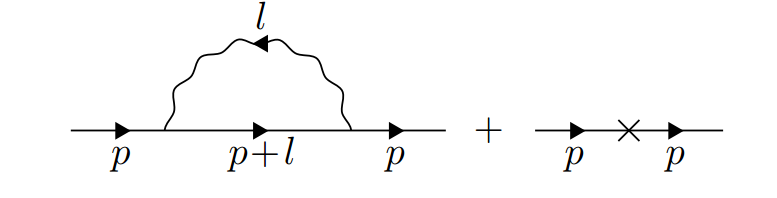
\includegraphics[scale=0.3]{QFT1/RG4.png}
\caption{Feynman diagram representation of two-particle scattering to one loop}
\end{figure}
\\
If we define $p = p_1 + p_2$, then the second diagram in the perturbation series is
\[\frac{(-i\lambda)^2}{2} \int \frac{d^4k}{(2\pi)^4} \frac{-i}{k^2+m^2} \frac{-i}{(k+p)^2+m^2} \equiv (-i\lambda)^2 iV(-p^2).\]
Thus the entire amplitude is therefore
\[i\mathcal{M} = -i\lambda + (-i\lambda)^2 [iV(s) + iV(t) + iV(u)] -i\delta_{\lambda} + \mathcal{O}(\lambda^3).\] 
To keep $\lambda$ dimensionless in dimensional regularization, we can make the transformation $\lambda \to \lambda \tilde{\mu}^{\epsilon}$. Here, $\tilde{\mu}$ is an arbitrary number with mass dimension 1 and $\epsilon \equiv 4-d$. We have
\[V(-p^2) = -\frac{1}{32\pi^2} \int_0^1 dx \left(\frac{2}{\epsilon} + \ln\left(\frac{\mu^2}{D(-p^2)}\right)\right),\]
where $\mu \equiv  \sqrt{4\pi} e^{-\gamma/2} \tilde{\mu}$, $D(-p^2) = x(1-x)p^2+m^2$.
The OS renormalization conditions imply that
\[\delta_{\lambda} = -\lambda^2[V(4m^2)+2V(0)] + \mathcal{O}(\lambda^3).\]
Thus
\[i\mathcal{M} = -i\lambda -\frac{i\lambda^2}{32\pi^2} \int_0^1 dx \left[\ln\left(\frac{D(s)}{D(4m^2)}\right) +\ln\left(\frac{D(t)}{D(0)}\right)+\ln\left(\frac{D(u)}{D(0)}\right)\right] + \mathcal{O}(\lambda^3).\]
To determine $\delta_Z$ and $\delta_m$ we must compute the two-point function. Define $-iM(p^2)$ as the sum of all one-particle-irreducible insertions into the propagator.The full two-point function is given by
\[\frac{-i}{p^2 + m^2 + M^2}.\]
The renormalization conditions require that the pole in this full propagator occur at $p^2=-m^2$ and have residue $1$. These two conditions are equivalent, respectively, to
\[M^2(p^2)|_{p^2=-m^2} = 0 , \quad \left. \frac{d}{dp^2} M^2(p^2)\right|_{p^2=-m^2} =0.\]
We can work out that
\[-iM^2(p^2) = \frac{i\lambda}{32\pi^2}\left(\frac{2}{\epsilon} + \ln\left(\frac{\mu^2}{m^2}\right)+1\right)m^2 -i(p^2\delta_Z + \delta_m).\]
Therefore, to the order of $\lambda$, 
\[\delta_Z=\mathcal{O}(\lambda^2) , \quad \delta_m = \frac{\lambda}{32\pi^2}\left(\frac{2}{\epsilon} + \ln\left(\frac{\mu^2}{m^2}\right)+1\right)m^2 + \mathcal{O}(\lambda^2) , \quad M^2(p^2) =\mathcal{O}(\lambda^2).\]
The detailed calculation can be found in chapter 10.2 of \emph{An introduction to quantum field theory (M.E.Peskin \& D.V.Schroeder)} and will be eliminated here.

\subsubsection{Perturbation theory to all orders}
We begin by summing all one-particle irreducible diagrams with two external lines; this gives us the self-energy $M^2$. We next sum all amputated diagrams with four external lines; this gives us the four-point vertex function $V_4(k_1, k_2, k_3, k_4)$. (We can prove that amputated diagrams with four external lines must be one-particle irreducible). Order by order in $\lambda$, we must adjust the value of the Lagrangian coefficients $\delta_Z$, $\delta_m$, and $\delta_{\lambda}$ to maintain the conditions $M^2(-m^2) = 0$, ${dM^2}/{dp^2}(-m^2) = 0$, and $V_4(s=4m^2) =0$. 
\\ \\
Next we will construct the $n$-point vertex functions $V_n$ with $4 < n \leq E$, where $E$ is the number of external lines in the process of interest. We compute these using a skeleton expansion. This means that we draw all the contributing 1PI diagrams, but omit diagrams that include either propagator or four-point vertex corrections. That is, we include only diagrams that are not only 1PI, but also 2PI and 4PI: they remain connected when any one, two, or four lines are cut. (Cutting four lines may isolate a single tree-level vertex, but nothing more complicated.) Then we take the propagators and vertices in these diagrams to be given by the exact propagator $-i / [(p^2+m^2+M^2(p^2)]$ and vertex $V_4(k_1,k_2,k_3,k_4)$, rather than by the tree-level propagator and vertex. We then sum these skeleton diagrams to get $V_n$ for $4 < n \leq E$. Order by order in $\lambda$, this procedure is
equivalent to computing $V_n$ by summing the usual set of contributing 1PI diagrams.
\\ \\
Next we draw all tree-level diagrams that contribute to the process of interest (which has $E$ external lines), including not only four-point vertices, but also $n$-point vertices. Then we evaluate these diagrams using the exact propagator for internal lines, and the exact 1PI vertices $V_n$; external lines are assigned a factor of one. We sum these tree diagrams to get the scattering amplitude. Order by order in $\lambda$, this procedure is equivalent to computing the scattering amplitude by summing the usual set of contributing diagrams.
Thus we now know how to compute an arbitrary scattering amplitude
to arbitrarily high order. The procedure is the same in any quantum field theory; only the form of the propagators and vertices change, depending on the spins of the fields.

\subsection{General renormalization theory}
Recall some of the major results and methods of renormalization theory:
\begin{enumerate}
\item In perturbation theory, bare and physical quantities are related by ultraviolet-divergent expressions
\[m_{\rm phys} = m_0 + \Delta_m,\]
where $m_{\rm phys}$ is finite, $\Delta_m$ is ultraviolet-divergent, and so $m_0$ is necessarily ultraviolet-divergent.
\item We express the Lagrangian in terms of physical quantites, and separate it into
\[\mathcal{L} = \mathcal{L}_0 + \mathcal{L}_{\rm I} + \mathcal{L}_{\rm CT},\]
where $\mathcal{L}_0$ is the canonically normalized free Lagrangian for physical fields and masses, $\mathcal{L}_{\rm I}$ contains the interaction, again in terms of physical parameters, and $\mathcal{L}_{\rm CT}$ contains the counterterms with ultraviolet divergent coefficients. From $\mathcal{L}_0$, we obtain the propagators of the physical fields. $\mathcal{L}_{\rm I}$ and $\mathcal{L}_{\rm CT}$ give
interaction vertices.
\item At the one-loop level, the self-energy is given by the effective two-point vertices: the 1PI two-point vertex of the interaction and the counter-term two-point vertex. The counterterms absorb ultraviolet divergences, and the finite parts of the counterterms are determined by renormalization conditions,
which ensure the quantities in $\mathcal{L}_0 + \mathcal{L}_{\rm I}$ are physical. The conditions constrain the self-energy and the effective vertices, and give a finite, uniquely-determined value for the counterterms.
\end{enumerate}
\subsubsection{Degrees of divergences}
Now, for a general theory in $d$ spacetime dimensions, the field content is given by $\phi_f$, $f=1,2,\cdots$, where $f$ labels
the field type. $[\phi_f]=\Delta f$ and $\Delta f > 0$ in all physical theories. We have interaction vertices of type $i$, $i = 1,2,\cdots$
contributing a term of the form
\[\lambda_i \partial^{n_i} \prod_f \phi_f^{n_{if}},\]
where $\lambda_i$ is the coupling constant, with dimension
\[[\lambda_i] = \kappa_i = d - n_i - \sum_f n_{if}\Delta f .\]
Now consider a 1PI diagram in such a theory:
\[E_f \equiv \mbox{ number of external lines of } \phi_f,\]
\[V_i \equiv \mbox{ number of vertices of type } i.\]
Then $M \sim \Lambda^D \prod_i \lambda_i ^{V_i}$ and so $D = [M] - \sum_i V_i \kappa_i$. Again
\[[M] - d = -\sum E_f \Delta f \]
and so the general expression for the superficial degree of divergence is given by
\[D = d - \sum_f E_f \Delta f - \sum_i V_i \kappa_i.\]
Diagrams which are ultraviolet divergent satisfy
\[\sum_f E_f \Delta f + \sum_i V_i \kappa_i < d.\]
We can now divide all theories into
\begin{enumerate}
\item All $\kappa_i > 0$: superrenormalizable theories.
\item All $\kappa_i \geq 0$: renormalizable theories.
\item There exists at least one $\delta_i < 0$: non-renormalizable theories.
\end{enumerate}
These terms also apply to individual interactions for a vertex of type $i$:
\begin{enumerate}
\item $\kappa_i > 0$: super-renormalizable, relevant interaction.
\item $\kappa_i \geq 0$ : renormalizable, marginal interaction.
\item $\kappa_i < 0$: non-renormalizable, irrelevant interaction.
\end{enumerate}

\subsubsection{Cancellation of divergences}
Consider a generic divergent diagram $M$ of degree $D$, that is,
\[M = \int^{\Lambda} ds s^{D-1}.\]
If all loop momenta are taken proportional to $s$. Generically, internal propagators have the form
\[\frac{1}{(as+p)^{\alpha}\cdots} \sim \frac{1}{s^{\alpha}}\]
for large $s$, where $a$ is a numerical constant and $p$ is a combination of the external momenta. Differentiating $M$, with respect to $p$, $n$ times gives a term proportional to
\[\frac{1}{(as+p)^{\alpha+n}} \sim \frac{1}{s^{\alpha + n}} \]
and so $D+1$ derivatives with respect to the external momenta will make $M$ finite. 
This means that
\[M(p) = M_0 + M_1 p + \cdots + M_D p^D + \mbox{ finite terms},\]
where the argument $p$ of the function represents the collection of external momenta, we have suppressed the index structure, and $M_0,M_1,\cdots,M_D$ are potentially divergent constants. Suppose that $M$ has $E_f$ external lines of the field $\phi_f$. Then divergences of $M(p)$ can be cancelled by counterterms of the form
\[\sum_{j=0}^D A_j (\partial)^j \prod_f \phi_f^{E_f},\]
where the $A_j$ are divergent coefficients in order to cancel divergences in $M_j$. 
The index structure in $A_j \partial^j$ should match the suppressed index structure of $M(p)$.

\section{Renormalization group}
\subsection{Modified minimal-subtraction scheme}
The Lagrangian of $\phi^4$ theory is
\[\mathcal{L} = -\frac{1}{2} \partial^{\mu} \phi \partial_{\mu} \phi -\frac{1}{2}m^2 \phi^2 - \frac{\lambda}{4!}\phi^4 -\frac{1}{2} \delta_Z \partial^{\mu} \phi \partial_{\mu} \phi -\frac{1}{2}\delta_m \phi_r - \frac{\delta \lambda}{4!}\phi^4.\]
For minimal-subtraction scheme, we do not demand that $m$ be the physics mass of the field and $\phi$  create a normalized one-particle state. The physical meaning of $\lambda$ is not expressed directly as well. Instead we choose $\delta_Z$, $\delta_m$ and $\delta_{\lambda}$ to cancel the infinities, and nothing more;
we say that $\delta_Z$, $\delta_m$ and $\delta_{\lambda}$ have no finite parts. It is called the modified minimal-subtraction or $\mathrm{\overline{MS}}$ scheme. (``modified'' because we introduced $\mu$ via  $\lambda \to \lambda \tilde{\mu}^{\epsilon}$, with $\mu \equiv  \sqrt{4\pi} e^{-\gamma/2} \tilde{\mu}$; had we set $\mu = \tilde{\mu}$ instead, the scheme would be just plain minimal subtraction or MS.)
\\ \\
For loop corrections to propagator,
\[\delta_Z=\mathcal{O}(\lambda^2) , \quad \delta_m = \left[ \frac{\lambda}{16\pi^2} + \mathcal{O}(\lambda^2) \right]\frac{1}{\epsilon}m^2 , \quad M^2(p^2) = \frac{\lambda}{32\pi^2}( \ln(\frac{m^2}{\mu^2})-1)m^2 + \mathcal{O}(\lambda^2).\]
Firstly, in the $\mathrm{\overline{MS}}$ scheme, the propagator will no longer have a pole at $k^2=-m^2$. The pole will be somewhere else. However, by definition, the actual physical mass $m_{\rm ph}$ of the particle is determined by the location of this pole: $k^2 = -m_{\rm ph}^2$. Thus, the Lagrangian parameter $m$ is no longer the same as $m_{\rm ph}$. The relation of $m$ and $m_{\rm ph}$ is 
\[m_{\rm ph}^2 = M^2(-m_{\rm ph}^2) + m^2.\]
To the lowest order, 
\[m_{\rm ph}^2 = \left[1+\frac{\lambda}{32\pi^2}( \ln(\frac{m^2}{\mu^2})-1)\right] m^2.\]
Because $m_{\rm ph}$ is a independent of $\mu$, according to $d m_{\rm ph} / d\mu = 0$, it can be derived that
\[\frac{dm}{d\ln \mu} = \left[\frac{\lambda}{32\pi^2}+\mathcal{O}(\lambda^2)\right] m.\]
Furthermore, the residue of this pole is no longer one. Let us call the residue $R$. Therefore, in the LSZ formula, we get a net factor of $\sqrt{R}$ for each external line when using the $\mathrm{\overline{MS}}$ scheme. And in $\phi^4$ theory,
\[R = 1 + \mathcal{O}(\lambda^2).\]
For loop corrections to vertex,
\[\delta_{\lambda} = \left[\frac{3\lambda^2}{16\pi^2} + \mathcal{O}(\lambda^3)\right]\frac{1}{\epsilon},\]
\[i\mathcal{M} = -i\lambda -\frac{i\lambda^2}{32\pi^2} \int_0^1 dx \left[\ln(\frac{D(s)}{\mu^2}) +\ln(\frac{D(t)}{\mu^2})+\ln(\frac{D(u)}{\mu^2})\right] + \mathcal{O}(\lambda^3).\]
For a process with $p^2 \gg m^2$, we have
\[ D \approx x(1-x)p^2.\]
In OS renormalization scheme, the one-loop correction to propagator or vertex generally includes a factor
\[\ln \left( \frac{D}{D_0}\right ) \sim \ln \frac{p^2}{m^2}.\]
Thus perturbation theory is no longer a good approximation when $p^2 \gg m^2$.
In $\overline{\rm MS}$ renormalization scheme, introducing $\mu$ allows us to address this problem: if we choose $\mu \sim p$, no such logarithm arises. 
If we choose $\mu$ appropriately, that is, to be comparable to the momentum scale of the physical process, we can improve our perturbation expansion. 
Thus $\lambda(\mu)$ and $m(\mu)$ can be considered as the scale-dependent coupling constants.
And the reason we get large logarithmic terms in the on-shell scheme is that we are trying to use coupling defined at one scale to describe physics at very different scales.

\subsection{Beta and gamma function}
\noindent
The Lagrangian of $\phi^4$ theory is 
\[\mathcal{L} = -\frac{1}{2} \partial^{\mu} \phi_0 \partial_{\mu} \phi_0 -\frac{1}{2}m_0^2 \phi_0^2 - \frac{\lambda_0}{4!}\phi_0^4.\]
It can be written as
\[\mathcal{L} = -\frac{1}{2}Z_{\phi} \partial^{\mu} \phi \partial_{\mu} \phi -\frac{1}{2}Z_{m}m^2 \phi^2 - Z_{\lambda} \tilde{\mu}^{\epsilon}\frac{\lambda}{4!}\phi^4.\]
Thus
\[\phi_0 = Z_{\phi}^{1/2}\phi , \quad m_0 = Z_{\phi}^{-1/2} Z_{m}^{1/2}m , \quad \lambda_0 = Z_{\phi}^{-2} Z_{\lambda} \lambda \tilde{\mu}^{\epsilon}.\]
After using dimensional regularization, the infinities coming from loop integrals take the form of inverse powers of $\epsilon$. In the  $\mathrm{\overline{MS}}$ renormalization scheme, we choose the $Z$s to cancel off these powers of $1/\epsilon$, and nothing more. Therefore the $Z$s can be written as
\begin{eqnarray}
Z_{\phi} = 1 + \sum_{n=1}^{\infty} \frac{a_n(\lambda)}{\epsilon^n} ,\nonumber \\
Z_{m} = 1 + \sum_{n=1}^{\infty} \frac{b_n(\lambda)}{\epsilon^n} ,\nonumber \\
Z_{\lambda} = 1 + \sum_{n=1}^{\infty} \frac{c_n(\lambda)}{\epsilon^n} .\nonumber 
\end{eqnarray}
In $\phi^4$ theory, $a_1 = \mathcal{O}(\lambda^2)$, $b_1 = {\lambda}/{16\pi^2} +  \mathcal{O}(\lambda^2)$, $c_1 = {3\lambda}/{16\pi^2} + \mathcal{O}(\lambda^2)$.
Remember that bare fields and parameters must be independent of $\mu$. 
Define
\[G(\lambda,\epsilon) \equiv \ln(Z_{\phi}^{-2} Z_{\lambda}) = \sum_{n=1}^{\infty} \frac{G_n(\lambda)}{\epsilon^n}.\]
We can work out $G_1 = c_1 - 2a_1 = {3\lambda}/{16\pi^2} + \mathcal{O}(\lambda^2)$.
As $\ln \lambda_0 = G + \ln \lambda + \epsilon \ln \tilde{\mu} $. 
From the independence of $\lambda_0$, we can derive
\[\left ( 1 + \frac{\lambda G'_1}{\epsilon} + \cdots \right) \frac{d\lambda}{d\ln \mu} + \epsilon \lambda = 0.\]
${d\lambda}/{d\ln\mu}$ is the rate at which $\lambda$ must change to compensate for a small change in $\ln \mu$. 
If compensation is possible at all, this rate should be finite in the $\epsilon \to 0$ limit. 
In a renormalizable theory, we should have
\[\frac{d\lambda}{d\ln\mu} = -\epsilon\lambda + \beta(\lambda).\]
Thus
\[\beta(\lambda) = \lambda^2 G'_1(\lambda).\]
In $\phi^4$ theory, we have
\[\beta(\lambda) = \frac{3\lambda^2}{16\pi^2} + \mathcal{O}(\lambda^3).\]
Define
\[M(\lambda,\epsilon) \equiv \ln(Z_{m}^{1/2} Z_{\phi}^{-1/2}) = \sum_{n=1}^{\infty} \frac{M_n(\lambda)}{\epsilon^n}.\]
We can work out that $M_1 = b_1/2 - a_1/2 = {\lambda}/{32\pi^2} + \mathcal{O}(\lambda^2)$.
As $\ln m_0 = M + \ln m $, define the anomalous dimension of the mass
\[\gamma_m(\lambda) \equiv \frac{1}{m} \frac{dm}{d \ln \mu}.\]
From the independence of $m_0$, we can derive that
\[\gamma_m(\lambda) = \lambda M'_1.\]
In $\phi^4$ theory, we have
\[\gamma_m(\lambda) = \frac{\lambda}{32\pi^2} + \mathcal{O}(\lambda^2).\]
We can expand $\ln Z_{\phi}$ as
\[\ln Z_{\phi} = \frac{a_1}{\epsilon} + \cdots \]
Define the anomalous dimension of the field
\[\gamma_{\phi}(\lambda) \equiv \frac{1}{2} \frac{d\ln Z_{\phi}}{d \ln \mu}.\]
We can derive
\[\gamma_{\phi}(\lambda) = -\frac{1}{2}\lambda a'_1.\]
In $\phi^4$ theory, we have
\[\gamma_{\phi}(\lambda) = \mathcal{O}(\lambda^2).\]

\subsection{Callen-Symanzik equation}
Consider the $n$ point green function,
\[G^{(n)}(x_1,\cdots,x_n) \equiv \langle \Omega | T \phi(x_1) \cdots \phi(x_n) | \Omega \rangle_C .\]
As $G^{(n)}_0 = Z_{\phi}^{n/2} G^{(n)}$, from the independence of bare Green's function, we have
\[\left( \frac{\partial}{\partial \ln \mu} + \beta(\lambda)  \frac{\partial}{\partial \lambda} + \gamma_m(\lambda) m  \frac{\partial}{\partial m} + n \gamma_{\phi}(\lambda)\right)G^{n}(x_1,\cdots,x_n;\lambda,m,\mu) = 0.\]
\\
From now on, we will focus on the $\phi^4$ theory in massless limit. Firstly, consider the two point Green's function in momentum space $G^{(2)}(p)$, we can express its dependence on $p$ and $\mu$ as
\[G^{(2)} = \frac{-i}{p^2} g(-p^2/\mu^2,\lambda(\mu)).\]
Then the C-S equation can be written as
\[\left[ p \frac{\partial}{\partial p} - \beta(\lambda)  \frac{\partial}{\partial \lambda} +2 - 2\gamma_{\phi}\right ] G^{(2)}(p,\lambda(\mu),\mu) = 0 ,\]
where $p \equiv (-p^2)^{1/2}$.
In the free theory, $\beta$ and $\gamma$ vanish and we recover the trivial result
\[G^{(2)}(p) = \frac{-i}{p^2}.\]
In an interacting theory, the solution to the C-S equation can be expressed as
\[G^{(2)}(p,\lambda_0,\mu_0) = G^{(2)}(\mu_0,\lambda_p,\mu_0)\exp \left (-\int_{p'=\mu_0}^{p'=p} d \ln(p'/\mu_0) \cdot 2[1-\gamma_{\phi}(\lambda_{p'})] \right ),\]
where $\lambda_0 = \lambda(\mu_0)$, $\lambda_p$ satisfy the following equation
\[\frac{\partial}{\partial \ln p} \lambda_p(p,\lambda_0) = \beta(\lambda_p) , \quad \lambda_p(\mu_0,\lambda_0) = \lambda_0.\]
The solution can be checked directly by noticing that
\[\left ( p \frac{\partial}{\partial p} - \beta(\lambda_0) \frac{\partial}{\partial \lambda_0} \right ) \lambda_p(p,\lambda_0) = 0.\]
A convenient way of writing the solution is
\[G^{(2)}(p,\lambda_0,\mu_0) =  \frac{-i}{p^2} g^{(2)}(\mu_0,\lambda_p,\mu_0)\exp \left (2\int_{\mu_0}^{p} d \ln(p'/\mu_0)  \gamma_{\phi}(\lambda_{p'}) \right ),\]
and $g(\lambda_p) = 1 + O(\lambda_p^2)$.
\\ \\
Now consider the connected four-point function of $\phi^4$ theory evaluated at spacelike momenta $p_i$ such that $p_i^2= P^2$, $p_i \cdot p_j = 0$, so that $s$, $t$, and $u$ are of order $-P^2$. 
To leading order in perturbation theory, this function is given by
\[G^{(4)}(P) = \left (\frac{i}{P^2}\right )^4 (-i\lambda).\]
The solution of C-S equation is
\[G^{(4)}(p,\lambda_0,\mu_0) =  \frac{1}{P^8} g^{(4)}(\mu_0,\lambda_p,\mu_0)\exp \left (4\int_{\mu_0}^{p} d \ln(p'/\mu_0)  \gamma_{\phi}(\lambda_{p'}) \right ),\]
and $g(\lambda_p) = -i\lambda_p + O(\lambda_p^2)$.
\\ \\
The ordinary Feynman perturbation series for a Green's function depends both on the coupling constant $\lambda$ and on the dimensionless parameter $\ln(p^2/\mu_0^2)$. The perturbation theory can be badly behaved even when $\lambda$ is small if the ratio $p^2/\mu_0^2$ is large. The solutions of C-S equation reorganize this dependence into a function of the running coupling constant and an exponential scale factor. 
The first factor of the solution is a function of the running coupling constant, evaluated at the momentum scale $p$. If $p$ were of order $\mu_0$, this function would essentially be the ordinary perturbation evaluation of the Green's function. We can make use of this same expression at the scale $p$, but to replace $\lambda_0$ with a new coupling constant $\lambda_p$ appropriate to that scale.
The exponential factor is the accumulated field strength rescaling of the correlation function from the reference point $\mu_0$ to the actual momentum $p$ at which the Green's function is evaluated. This factor receives a multiplicative contribution from each intermediate scale between $\mu$ and $p$.
\\ \\
In $\phi^4$ theory, we have
\[\frac{d}{d\ln p} \lambda_p = \frac{3\lambda_p^2}{16\pi^2}.\]
The solution is
\[\lambda_p = \frac{\lambda_0}{1 - \frac{3\lambda_0}{16\pi^2} \ln (p/\mu_0)}.\]
This expression for the running coupling constant goes to zero at a logarithmic rate as $p \to 0$. If we expand the running coupling constant $\lambda_p$ in powers of $\lambda_0$, we find that the successive powers of the coupling constant are multiplied by powers of logarithms, 
\[\lambda_0^{n+1}(\ln p/\mu_0)^n,\]
which become large and invalidate a simple perturbation expansion for $p$ much greater or much less than $\mu_0$. If the running coupling constant becomes large, as happens in $\phi^4$ theory for $p \to \infty$, the perturbation expansion will break down anyway, and we will need more advanced methods. However, if the running coupling constant becomes small, as for $\phi^4$ theory as $p \to 0$, we will have successfully organized the powers of logarithms into a meaningful and controlled expression.

\subsection{Running of coupling constants}
In the limit of $\epsilon \to 0$, the coupling constant satisfies the differential equation
\[\frac{\partial \lambda}{\partial \ln \mu} = \beta(\lambda).\]
Three behaviours are possible in the region of small $\lambda$:
\begin{enumerate}
\item $\beta(\lambda) > 0$.
\item $\beta(\lambda) = 0$.
\item $\beta(\lambda) < 0$.
\end{enumerate}
\noindent
In theories of the first class, the running coupling constant goes to zero in the infra-red, leading to definite predictions about the small-momentum behaviour of the theory. However, the running coupling constant becomes large in the region of high momenta. Thus the short-distance behaviour of the theory cannot be computed using Feynman diagram perturbation theory.A Feynman diagram analysis is useful in such theories if one is mainly interested in large-distance or macroscopic behaviour.
\\ \\
In theories of the second class, the coupling constant does not flow. In these theories, the running coupling constant is independent of the momentum scale, and thus equal to the bare coupling. This means that there can be no ultraviolet divergences in the relation of coupling constants. The only possible ultraviolet divergences in such theories are those associated with field rescaling, which automatically cancel in the computation of S-matrix elements. Such theories are called finite quantum field theories. Before the emergence of our modern understanding of renormalization, these theories would have been embraced as the solution to the problem of ultraviolet infinities. But in fact the known finite field theories in four dimensions are very special constructions the so-called gauge theories with extended supersymmetry with no known physical application. 
\\ \\
In theories of the third class, the running coupling constant becomes large in the large-distance regime and becomes small at large momenta or short distances. Such theories are called asymptotically free. In theories of this class, the short-distance behaviour is completely solvable by Feynman diagram methods. Though ultraviolet divergences appear in every order of perturbation theory, the renormalization group tells us that the sum of these divergences is completely harmless.
\\ \\
In the region of strong coupling, the approximation we have made, ignoring the higher-order terms in the $\beta$ function is no longer valid. It is a logical possibility that the leading order term is positive while the higher terms of the $\beta$ function are negative, so that the $\beta$ function has a zero at a non-zero value $\lambda_*$. When $\lambda_*$ approaches this value, the renormalization group flow slows to a halt; thus $\lambda = \lambda_*$ would be a non-trivial fixed point of the renormalization group. 
If the $\beta$ function behaves in the vicinity of the fixed point as 
\[\beta \approx -B(\lambda - \lambda_*),\] 
where $B$ is a positive constant. For $\lambda$ near $\lambda_*$ 
\[\frac{d}{d\ln \mu} \lambda \approx -B(\lambda-\lambda_*).\]
The solution of this equation is
\[\lambda(\mu) = \lambda_* + C(\frac{\mu_0}{\mu})^B.\]
Thus, $\lambda$ indeed tends to $\lambda_*$ as $\mu \to \infty$, and the rate of approach is governed by the slope of the $\beta$ function at the fixed point. The fixed point here is called ultraviolet-stable fixed point. 
If $p$ is sufficiently large, $\lambda(p)$ is close to $\lambda_*$.In the massless limit, the solution of C-S equation for two point Green function in momentum space becomes
\[G^{(2)}(p,\lambda_0,\mu_0) \approx G^{(2)}(\mu_0,\lambda_*,\mu_0)\exp \left (- \ln(p/\mu_0) \cdot 2[1-\gamma_{\phi}(\lambda_*)] \right ).\]
Thus the naive scaling law $G(p) \sim p^{-2}$ is changed to $G(p) \sim p^{-2[1-\gamma_{\phi}(\lambda_*)]}$. This has applications in the theory of critical phenomena.
A similar behaviour is possible in an asymptotically free theory. If the $\beta$ function behaves in the vicinity of the fixed point as 
\[\beta \approx B(\lambda - \lambda_*),\] 
where $B$ is a positive constant.
the running coupling constant will tend to a fixed point as $\mu \to 0$.  The fixed point is called infrared-stable fixed points. 

\section{Spontaneous symmetry breaking}
\subsection{Effective action}
\[Z[J] = e^{-iE[J]} = \int \mathcal{D} \phi \exp\left[ i\int d^4x (\mathcal{L}[\phi] + J \phi) \right].\]
Define 
\[\phi_{\rm cl} (x) \equiv \langle \Omega | \phi(x) | \Omega \rangle_{J}.\]
Therefore, we can derive
\[\frac{\delta}{\delta J(x)} E[J] = - \phi_{\rm cl}(x).\]
Define effective action as
\[\Gamma[\phi_{\rm cl}] \equiv -E[J] - \int d^4y J(y) \phi_{\rm cl}(y).\]
Suppose $\mathcal{L}$ is invariant under transformation $U$, i.e. $\mathcal{L}(U\phi) = \mathcal{L}(\phi) $. Then we can prove that effective action $\Gamma$ is also invariant under transformation $U$, i.e. $\Gamma(U\phi_{\rm cl}) = \Gamma(\phi_{\rm cl}) $.

\begin{newproof}
\[ U\phi_{\rm cl}(x) = \langle \Omega | U\phi(x) | \Omega\rangle_{J} = \frac{\int \mathcal{D}\phi e^{i \int \mathcal{L}(\phi)+J\phi}U\phi(x)}{\int \mathcal{D}\phi e^{i \int \mathcal{L}(\phi)+J\phi}}.\]
Define $J' = \frac{J\phi}{U\phi}$,  and we suppose the measure of path integral is invariant under transformation $U$, then we have
\[ U\phi_{\rm cl}(x) = \frac{\int \mathcal{D}U\phi e^{i \int \mathcal{L}(U\phi)+J'U\phi}U\phi(x)}{\int \mathcal{D}U\phi e^{i \int \mathcal{L}(U\phi)+J'U\phi}} =  \frac{\int \mathcal{D}\phi e^{i \int \mathcal{L}(\phi)+J'\phi}\phi(x)}{\int \mathcal{D}\phi e^{i \int \mathcal{L}(\phi)+J'\phi}} = \langle \Omega | \phi(x) | \Omega\rangle_{J'}.\]
On the one hand, we have
\[\Gamma[U\phi_{\rm cl}] = E[J'] - \int d^4y J'(y)U\phi_{\rm cl}(y) =  E[J'] - \int d^4y J(y)\phi_{\rm cl}(y).\]
On the other hand, we have
\begin{eqnarray}
Z[J'] &=& \int \mathcal{D}\phi \exp \left[ i \int d^4x \mathcal{L}(\phi)+J'\phi \right] =  \int \mathcal{D}U\phi \exp \left[ i \int d^4x \mathcal{L}(U\phi)+J'U\phi \right] \nonumber
\\
&=& \int \mathcal{D}\phi \exp \left[ i \int d^4x \mathcal{L}(\phi)+J\phi \right] = Z[J] .\nonumber
\end{eqnarray}
Thus $\Gamma(U\phi_{\rm cl}) = \Gamma(\phi_{\rm cl})$.
\end{newproof}

\noindent
We can further verify that
\[\frac{\delta}{\delta \phi_{\rm cl}(x)} \Gamma[\phi_{\rm cl}] = -J(x).\]
If the external source is set to zero, the effective action satisfy the equation
\[\frac{\delta}{\delta \phi_{\rm cl}(x)} \Gamma[\phi_{\rm cl}] = 0.\]
The solution to this equation are the values of $\langle \phi(x) \rangle$ in the stable quantum states of the theory. For a translational-invariant vacuum state, we will find a solution in which $\phi_{\rm cl}$ is independent of $x$. For simplicity, will assume the vacuum state in our following discussion are all translational-invariant. 
Therefore, if $T$ is the time extent of the region and $V$ is its three dimensional volume, we can define the effective potential of the field by
\[\Gamma[\phi_{\rm cl}] = -(VT) \cdot V_{\rm eff}(\phi_{\rm cl}).\]
The condition that $\Gamma[\phi_{\rm cl}]$ has an extreme then reduces to the simple equation
\[\frac{\partial}{\partial \phi_{\rm cl}} V_{\rm eff}(\phi_{\rm cl}) = 0.\] 
A system with spontaneously broken symmetry will have several minimum of $V_{\rm eff}$, all with the same energy by virtue of the symmetry. The choice of one among these vacuum is the spontaneous symmetry breaking.

\subsection{Computation of the effective action}
Decompose the Lagrangian into a piece depending on renormalized parameters and one containing the counter-terms
\[\mathcal{L} = \mathcal{L}_1 + \delta \mathcal{L}.\]
Define $J_1$ by
\[\left. \frac{\delta \mathcal{L}_1}{\delta \phi} \right|_{\phi = \phi_{\rm cl}} + J_1(x) = 0.\]
Define $\delta J$ by
\[J(x) = J_1(x) + \delta J(x).\]
Thus we have
\[e^{-iE[J]} = \int \mathcal{D}\phi e^{i\int d^4x (\mathcal{L}_1 + J_1\phi)} e^{i\int d^4x (\delta \mathcal{L} + \delta J \phi)}.\]
Replace $\phi$ by $\phi_{\rm cl}+\eta$,
\begin{eqnarray}
\int d^4x \, (\mathcal{L}_1 + J_1\phi) &=& \int d^4x \, (\mathcal{L}_1[\phi_{\rm cl}] + J_1\phi_{\rm cl}) + \int d^4x \, \eta(x) \left( \frac{\delta \mathcal{L}_1}{\delta \phi} + J_1 \right) \nonumber \\
&+& \frac{1}{2} \int d^4x \, d^4y \, \eta(x) \eta(y) \frac{\delta^2 \mathcal{L}_1}{\delta \phi(x) \delta \phi(y)} \nonumber \\
&+& \frac{1}{3!} \int d^4x \, d^4y \, d^4z \, \eta(x) \eta(y) \eta(z) \frac{\delta^3 \mathcal{L}_1}{\delta \phi(x) \delta \phi(y) \delta \phi(z)} + \cdots \nonumber
\end{eqnarray}
The term linear in $\eta$ vanishes by definition of $J_1$. 
Then, put back the effects of the counter-term Lagrangian,writing it as
\[(\delta \mathcal{L}[\phi_{\rm cl}] + \delta J \phi_{\rm cl} ) + ( \delta \mathcal{L}[\phi_{\rm cl} + \eta] - \delta\mathcal{L} [\phi_{\rm cl}] + \delta J \eta).\]
Define
\[\mathcal{L}_2 = \left(\frac{1}{3!} \int d^4x \, d^4y \, d^4z \, \eta(x) \eta(y) \eta(z) \frac{\delta^3 \mathcal{L}_1}{\delta \phi(x) \delta \phi(y) \delta \phi(z)} + \cdots \right) + ( \delta \mathcal{L}[\phi_{\rm cl} + \eta] - \delta\mathcal{L} [\phi_{\rm cl}] + \delta J \eta).\]
Thus
\[e^{-iE[J]} = C_1 e^{i\int \mathcal{L}_2(\frac{1}{i} \frac{\delta}{\delta I})} \left. \int \mathcal{D}\eta e^{i\int \left(\frac{1}{2} \eta \frac{\delta^2 \mathcal{L}_1}{\delta \phi \delta \phi} \eta + I\eta \right)} \right|_{I=0},\]
where
\[C_1 \equiv \exp \left[ i \int ( \mathcal{L}_1 [\phi_{\rm cl}] + J_1\phi_{\rm cl} + \delta \mathcal{L}[\phi_{\rm cl}] + \delta J \phi_{\rm cl} )\right].\]
If we define propagator $D_{\rm F}$ as
\[D_{\rm F} \equiv i \left( \frac{\delta^2 \mathcal{L}_1}{\delta \phi \delta \phi}\right)^{-1}.\]
We have
\[Z[J] = e^{-iE[J]} =C_1 Z_0[0] e^{i\int \mathcal{L}_2(\frac{1}{i} \frac{\delta}{\delta I})} \left. \int \mathcal{D}\eta e^{i\int \left(-\frac{1}{2} I D_{\rm F} I \right)} \right|_{I=0},\]
where
\[Z_0[0] \equiv \int \mathcal{D}\eta e^{ \frac{i}{2}\int \eta \left( \frac{\delta^2 \mathcal{L}_1}{\delta \phi \delta \phi}\right) \eta }.\]
Similar to the procedure in the perturbation theory for path integral quantization, we can get a perturbation expansion for $iE[J]$ using connected Feynman diagram,
\[-iE[J] = i \int ( \mathcal{L}_1 [\phi_{\rm cl}] + J_1\phi_{\rm cl} + \delta \mathcal{L}[\phi_{\rm cl}] + \delta J \phi_{\rm cl} ) + \log(Z_0[0]) + \mbox{ connected diagrams }.\]
From this equation, $\Gamma$ follows directly:
\[\Gamma[\phi_{\rm cl}] = \int d^4x \mathcal{L}_1[\phi_{\rm cl}] -i\log(Z_0[0]) -i \mbox{ connected diagrams} + \int d^4x \delta\mathcal{L}[\phi_{\rm cl}].\]
Notice that there are no terms remaining that depend explicitly on $J$; thus, $\Gamma$ is expressed as a function of $\phi_{\rm cl}$ , as it should be. The Feynman diagrams contributing to $\Gamma[\phi_{\rm cl}]$ have no external lines, and the simplest ones turn out to have two loops. The lowest-order quantum correction to $\Gamma$ is given by the
functional determinant.
The last term provides a set of counter-terms that can be used to satisfy the renormalization conditions on $\Gamma$ and, in the process, to cancel divergences that appear in the evaluation of the functional determinant and the diagrams. 
The renormalization conditions will determine all of the counter-terms in $\delta \mathcal{L}$. However, the formalism we have constructed contains a new counter-term $\delta J$. That coefficient is determined by  $\langle \eta \rangle = 0$. In practice, we will satisfy this condition by simply ignoring any one-particle-irreducible one-point diagram, since any such diagram will be cancelled by adjustment of $\delta J$.

\subsection{The effective action as a generating functional}
$E[J]$ is called the generating of connected correlation functions,
\[\frac{\delta^n E[J]}{\delta J(x_1) \cdots \delta J(x_n)} = i^{n+1} \langle \phi(x_1) \cdots \phi(x_n) \rangle_{\mbox{conn}}.\]
The effective action $\Gamma[\phi_{\rm cl}]$ is the generating functional of one-particle-irreducible correlation functional,
\[\frac{\delta \Gamma[\phi_{\rm cl}]}{\delta \phi_{\rm cl}(x)}  = 0,\]
\[\frac{\delta^2 \Gamma[\phi_{\rm cl}]}{\delta \phi_{\rm cl}(x) \delta \phi_{\rm cl}(y)}  = iD^{-1}(x,y),\]
where $D(x,y) = \langle \phi(x) \phi(y) \rangle_{\mbox{conn}}$. 
When $n \geq 3$,
\[\frac{\delta^n \Gamma[\phi_{\rm cl}]}{\delta \phi_{\rm cl}(x_1) \cdots \delta \phi_{\rm cl}(x_n)} = -i \langle \phi(x_1) \cdots \phi(x_n) \rangle_{\mbox{1PI}}.\]
The proof of statements above can be found in chapter 10.2 of \emph{An introduction to quantum field theory (M.E.Peskin \& D.V.Schroeder)}
\\ \\
The chapter 21 of \emph{Quantum field theory (M. Srednicki)} gives an constructive way to define the effective action.
\begin{eqnarray}
\Gamma[\phi] & \equiv & \frac{1}{2} \int \frac{d^d k}{(2\pi)^d} \tilde{\phi}(-k)(-k^2 - m^2 - M^2(k^2))\tilde{\phi}(k) \nonumber \\
& + & \frac{1}{n!} \int \frac{d^d k_1}{(2\pi)^d} \cdots \frac{d^d k_n}{(2\pi)^d} (2\pi)^d \delta(k_1+\cdots+k_n) V_n(k_1,\cdots,k_n) \tilde{\phi}(k_1) \cdots \tilde{\phi}(k_n) ,\nonumber
\end{eqnarray}
where $\tilde{\phi}(k) = \int d^dx e^{-ikx} \phi(x)$, and $iV_n(k_1,\cdots,k_n)$ equals the value of 1PI Feynman diagram in momentum space. The effective action has the property that the tree-level Feynman diagrams it generates give the complete scattering amplitude of the original theory. The author also proved that this definition is equivalent to the definition from \emph{An introduction to quantum field theory (M.E.Peskin \& D.V.Schroeder)}.

\subsection{Renormalization and symmetry}
Consider first the computation of the effective potential for constant classical fields, in a field theory with an arbitrary number of fields $\phi^i$. The effective potential has mass dimension $4$, so we expect that $V_{\rm eff}(\phi_{\rm cl})$ will have divergent terms up to $\Lambda^4$. To understand these divergences,
expand $V_{\rm eff}(\phi_{\rm cl})$ in a Taylor series:
\[V_{\rm eff}(\phi_{\rm cl}) = A_0 + A_2^{ij}\phi_{\rm cl}^i \phi_{\rm cl}^j + A_4^{ijkl} \phi_{\rm cl}^i \phi_{\rm cl}^j \phi_{\rm cl}^k \phi_{\rm cl}^l + \cdots\]
In theories without a symmetry of $\phi \to -\phi$, there might also be terms linear and cubic in $\phi^i$; we omit these for simplicity. The coefficients $A_0$, $A_2$, $A_4$ have mass dimension, respectively, $4$, $2$, and $0$; thus we expect them to contain $\Lambda^4$, $\Lambda^2$, and $\log \Lambda$ divergences, respectively. The power-counting analysis predicts that all higher terms in the Taylor series expansion should be finite.
\\ \\
The constant term $A_0$ is independent of $\phi_{\rm cl}$; it has no physical significance. However, the divergences in $A_2$ and $A_4$ appear in physical quantities, since these coefficients enter the inverse propagator and the irreducible four-point function and therefore appear in the computation of S-matrix elements. There is one further coefficient in the effective action that has non-negative mass dimension by power counting; this is the coefficient of the term quadratic in $\partial_{\mu} \phi_{\rm cl}$, which appears when the effective action is evaluated for a non-constant background field:
\[\Delta \Gamma [\phi_{\rm cl}] = \int d^4x B_2^{ij} \partial_{\mu} \phi_{\rm cl}^i \partial^{\mu} \phi_{\rm cl}^j.\]
All other coefficients in the Taylor expansion of the effective action in powers of $\phi_{\rm cl}$ are finite by power counting.
\\ \\
We can now argue that the counter-terms of the original Lagrangian suffice to remove the divergences that might appear in the computation of $\Gamma[\phi_{\rm cl}]$. The argument proceeds in two steps. We first use the BPHZ theorem to argue that the divergences of Green's functions can be removed by adjusting a set of counter-terms corresponding to the possible operators that can be added to the Lagrangian with coefficients of mass dimension greater than or equal to zero. The coefficients of these counter-terms are in 1-to-1 correspondence with the coefficients $A_2$, $A_4$, and $B_2$ of the effective action. Next, we use the fact that the effective action is manifestly invariant to the original Symmetry group of the model. This is true even if the vacuum state of the model has spontaneous symmetry breaking, since the method we presented for computing the effective action is manifestly invariant to the original symmetry of the Lagrangian. Combining these two results, we conclude that the effective action can always be made finite by adjusting the set of counter-terms that are invariant to the original symmetry of the theory, even if this symmetry is spontaneously broken.

\subsection{Goldstone's theorem}
\begin{newthem}[Goldstone's theorem]
Goldstone's theorem examines a generic continuous symmetry which is spontaneously broken; i.e., its currents are conserved, but the ground state is not invariant under the action of the corresponding charges. Then, necessarily, new massless (or light, if the symmetry is not exact) scalar particles appear in the spectrum of possible excitations. There is one scalar particle - called a Nambu-Goldstone boson — for each generator of the symmetry that is broken, i.e., that does not preserve the ground state.
\end{newthem}
\begin{newproof}
A general continuous symmetry transformation has the form
\[\phi^a \to \phi^a + \alpha \Delta^a (\phi),\]
where $\alpha$ is an infinitesimal parameter and $\Delta^a$ is some function of all the $\phi$'s. Specialize to constant fields; then the derivative terms in $\mathcal{L}$ vanish and the potential alone must be invariant. This condition can be written
\[V(\phi^a) = V(\phi^a + \alpha \Delta^a (\phi)) , \quad \mbox{or} , \quad \Delta^a(\phi) \frac{\partial}{\partial \phi^a} V(\phi) = 0.\]
The effective potential $V_{\rm eff}$ encapsulates the full solution to the theory, including all orders of quantum corrections. At the same time, it satisfies the general properties of the classical potential: It is invariant to the symmetries of the theory, and its minimum gives the vacuum expectation value of $\phi_{\rm cl}$. Thus
\[\Delta^a(\phi) \frac{\partial}{\partial \phi^a} V_{\rm eff}(\phi) = 0.\]
Now differentiate with respect to $\phi^b$, and set $\phi = \phi_{\rm cl}$
\[0 = \left( \frac{\partial \Delta^a}{\partial \phi^b} \right)_{\phi_{\rm cl}} \left( \frac{\partial V_{\rm eff}}{\partial \phi^a}\right)_{\phi_{\rm cl}} + \Delta^a(\phi_{\rm cl}) \left( \frac{\partial^2}{\partial \phi^a \partial \phi^b}V_{\rm eff}\right)_{\phi_{\rm cl}}.\]
The first term vanishes since $\phi_{\rm cl}$ is a minimum of $V_{\rm eff}$, so the second term must also vanish. If the transformation leaves $\phi_{\rm cl}$ unchanged (i.e., if the symmetry is respected by the ground state), then $\Delta^a(\phi_{\rm cl})=0$ and this relation is trivial. A spontaneously broken symmetry is precisely one for which $\Delta^a(\phi_{\rm cl}) \neq 0$; in this
case $\Delta^a(\phi_{\rm cl})$ is the vector with eigenvalue zero.
We now argue that the presence of such a zero eigenvalue implies the existence of a massless scalar particle. Effective action's second functional derivative is the inverse propagator
\[i\tilde{D}_{ij}^{-1}(p^2) = \int d^4x e^{-ip(x-y)} \left. \frac{\delta \Gamma}{\delta \phi^i \delta \phi^j}(x,y) \right|_{\phi = \phi_{\rm cl}}.\]
A particle of mass $0$ corresponds to a zero eigenvalue of this matrix equation at $p^2 = 0$. Now set $p=0$. This implies $\frac{\delta \Gamma}{\delta \phi^i \delta \phi^j}(x,y)$ has a zero eigenvalue. This is equivalent to 
\[\frac{\partial^2}{\partial \phi^i_{\mathrm{cl}} \partial \phi^j_{\mathrm{cl}}}V_{\rm eff}\]
has a zero eigenvalue. This completes the proof of Goldstone's theorem.
\end{newproof}

\section{Linear sigma model}
\subsection{Introduction}
\[\mathcal{L} = -\frac{1}{2} \partial_{\mu} \phi^i \partial^{\mu}\phi^i + \frac{1}{2} \mu^2 (\phi^i)^2 - \frac{\lambda}{4} [(\phi^i)^2]^2.\]
The Lagrangian is invariant under the symmetry
\[\phi^i \to R^{ij} \phi^j\]
for any $N \times N$ orthogonal group in $N$ dimensions, also called the $N$-dimensional orthogonal group or simply $O(N)$. In classical theory, the lowest-energy classical configuration is a constant field $\phi_0^i$, whose value is chosen to minimize the potential
\[V = -\frac{1}{2}\mu^2 (\phi^i)^2 + \frac{\lambda}{4}[(\phi^i)^2]^2.\]
This potential is minimized for any $\phi_0^i$ that satisfies
\[(\phi^i)^2 = \frac{\mu^2}{\lambda} .\]
This condition determines only the length of the vector $\phi_0^i$, its direction is arbitrary. 
It is conventional to choose coordinates so that $\phi_0^i$ points in the $N$th direction
\[\phi_0^i = (0,0,\cdots,0,v) , \quad v \equiv \frac{\mu}{\sqrt{\lambda}}.\]
We can now define a set of shifted fields by writing
\[\phi^i = (\pi^k,v+\sigma) , \quad k = 1,\cdots,N-1.\]
It is now straightforward to rewrite the Lagrangian in terms of the $\pi$ and $\sigma$ fields. The result is
\begin{eqnarray}
\mathcal{L} &=& -\frac{1}{2}(\partial_{\mu}\pi^k)^2 - \frac{1}{2}(\partial_{\mu}\sigma)^2 - \frac{1}{2}(2\mu^2)\sigma^2 \nonumber \\
&-& \sqrt{\lambda}\mu \sigma^3 - -\sqrt{\lambda}\mu (\pi^k)^2\sigma - \frac{\lambda}{4}\sigma^4 - \frac{\lambda}{2}(\pi^k)^2\sigma^2 - \frac{\lambda}{4}[(\pi^k)^2]^2 .\nonumber
\end{eqnarray}
We obtain a massive $\sigma$ field and also a set of $N-1$ massless $\pi$ fields. The original $O(N)$ symmetry is hidden when we choose a specific $\phi_0^i$ for vacuum state, leaving only the subgroup $O(N-1)$, which rotates the $\pi$ fields among themselves. Given the Goldstone's theorem, our discussion here will remain valid when quantum correction is considered.

\subsection{Renormalization}
From this expression of the Lagrangian written in terms of shifted fields, we can read off the Feynman rules for the linear sigma model. Then we can compute tree-level amplitudes without difficulty.
\\
\begin{figure}[!h]
\centering
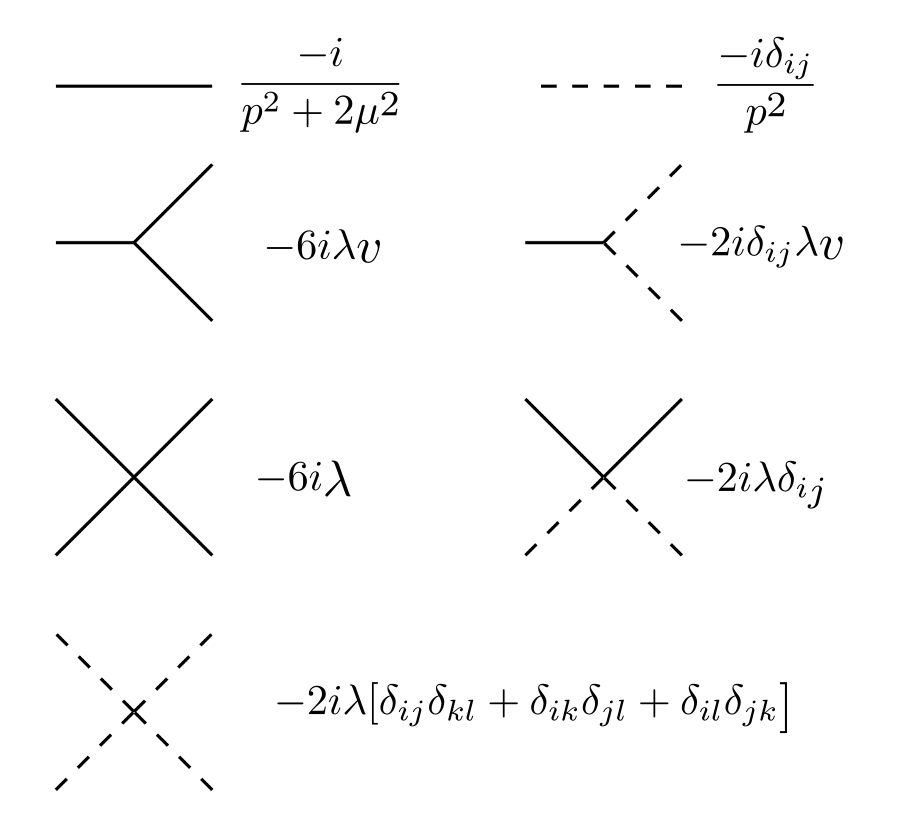
\includegraphics[scale=0.2]{QFT1/Li_sigma1.png}
\caption{Feynman rules for the linear sigma model}
\end{figure}
\\
Diagrams with loops, however, will often diverge. For the amplitude with $N_e$ external legs, the superficial degree of divergence is
\[D = 4 - N_e.\]
The linear sigma model has eight different superficially divergent amplitudes and several of these have $D > 0$ and therefore can contain more than one infinite constant.
\\
\begin{figure}[!h]
\centering
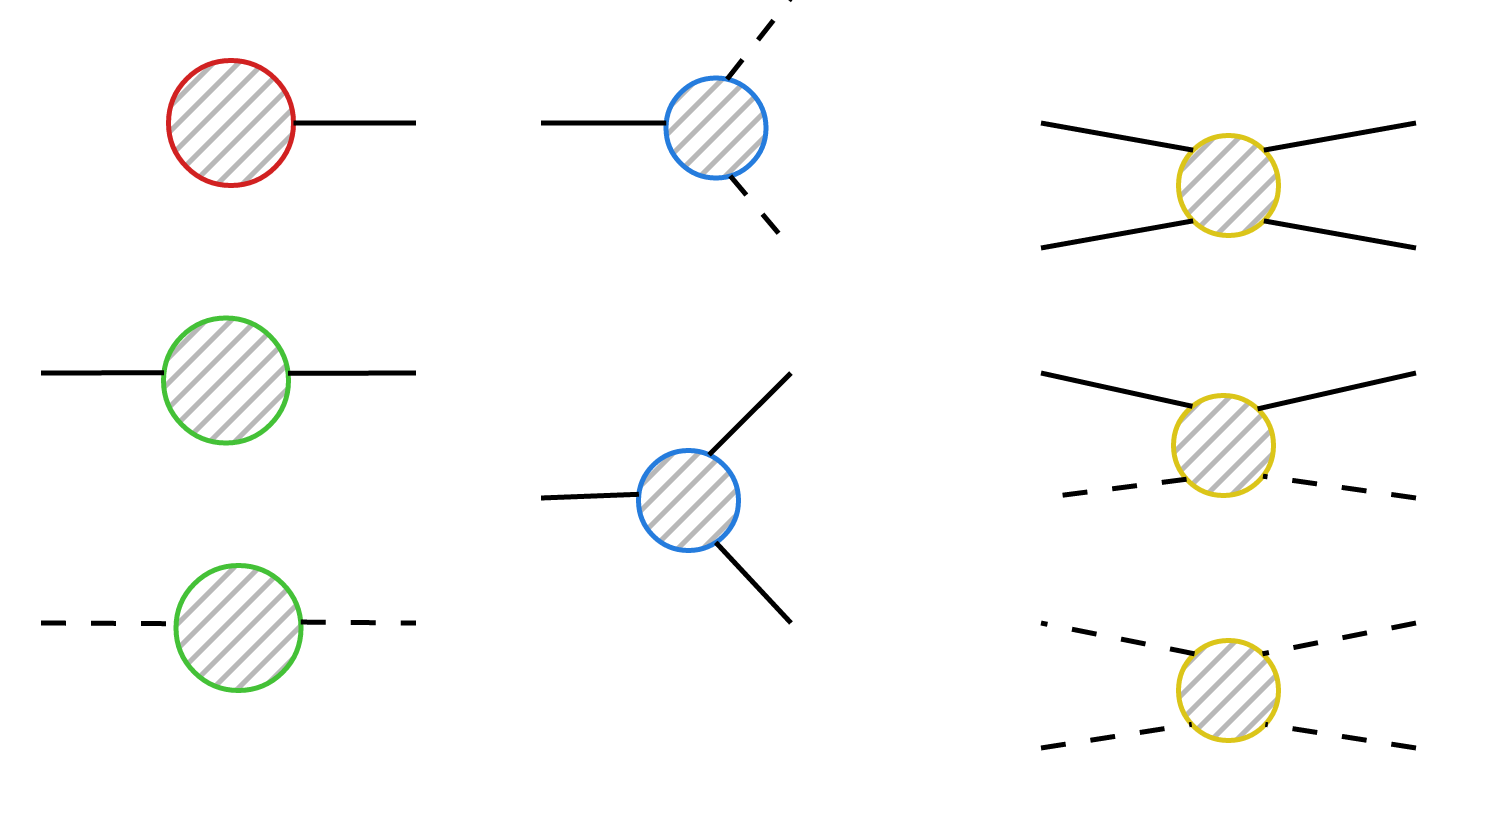
\includegraphics[scale=0.2]{QFT1/Li_sigma2.png}
\caption{Divergent amplitudes in the linear sigma model}
\end{figure}
\\
Yet we have only three counterterms:
\[\mathcal{L}_{ct} = -\frac{1}{2} \delta_Z \partial_{\mu} \phi^i \partial^{\mu}\phi^i - \frac{1}{2} \delta_{\mu} (\phi^i)^2 - \frac{\delta_{\lambda}}{4} [(\phi^i)^2]^2 .\]
Written in terms of $\sigma$ and $\pi$ fields, we have
\begin{eqnarray}
\mathcal{L}_{ct} &=& -\frac{\delta_Z}{2}(\partial_{\mu}\pi^k)^2 - \frac{1}{2}(\delta_{\mu}+\delta_{\lambda}v^2)(\pi^k)^2 -\frac{\delta_Z}{2}(\partial_{\mu}\sigma)^2 - \frac{1}{2}(\delta_{\mu} + 3\delta_{\lambda}v^2)\sigma^2 \nonumber \\
&-& (\delta_{\mu}v + \delta_{\lambda}v^3)\sigma - \delta_{\lambda}v\sigma(\pi^k)^2 - \delta_{\lambda}v\sigma^3 - \frac{\delta_{\lambda}}{4}[(\pi^k)^2]^2 - \frac{\delta_{\lambda}}{2}\sigma^2 (\pi^k)^2 - \frac{\delta_{\lambda}}{4}\sigma^4 .\nonumber
\end{eqnarray}
We can get the Feynman rules associated with these counterterms and set renormalization conditions for linear sigma model.
\begin{figure}[!h]
\centering
\includegraphics[height=5cm ,width=11.46cm]{QFT1/Li_sigma3.png}
\caption{Feynman rules for counterterm vertices in the linear sigma model}
\end{figure}
\begin{figure}[!h]
\centering
\includegraphics[height=3cm ,width=7.2cm]{QFT1/Li_sigma4.png}
\caption{Renormalization conditions ($m^2 = 2\mu^2$)}
\end{figure}
One-loop corrections for linear sigma model has been calculated in section 11.2 of \emph{An introduction to quantum field theory (M.E.Peskin \& D.V.Schroeder)}. There are two important results:
\begin{itemize}
\item All the divergence up to one loop will be cancelled by adjusting three counterterms. Apparently, the divergent part of the diagram is unaffected by the symmetry breaking.
\item The propagator of $\pi\pi$ has a pole at $p^2 = 0$ after one loop correction, i.e. $\pi$ particles remain massless after one loop correction.
\end{itemize}

\subsection{Effective action}
We begin again with the Lagrangian
\[\mathcal{L}_1 = -\frac{1}{2} \partial_{\mu} \phi^i \partial^{\mu}\phi^i + \frac{1}{2} \mu^2 (\phi^i)^2 - \frac{\lambda}{4} [(\phi^i)^2]^2.\]
Expand about the classical field $\phi^i = \phi_{\rm cl}^i + \eta^i$, and we assume the vacuum is translational invariant. Then we have
\[\mathcal{L}_1 = -\frac{1}{2}(\partial_{\mu}\eta)^2 + \frac{1}{2}\mu^2(\eta^i)^2 - \frac{\lambda}{2}[(\phi_{\rm cl}^2)(\eta^i)^2+ 2(\phi_{\rm cl}^i\eta^i)^2] + \cdots\]
From the terms quadratic in $\eta$, we can read off
\[\frac{\delta^2 \mathcal{L}_1}{\delta\phi^i\delta\phi^j} = \partial^2\delta_{ij} + \mu^2\delta_{ij} - \lambda[(\phi_{\rm cl}^k)^2\delta_{ij} + 2\phi_{\rm cl}^i \phi_{\rm cl}^j].\]
We choose the vacuum state by demanding $\phi_{\rm cl}^i$ points in the $N$th direction
\[\phi_{\rm cl}^i = (0,\cdots,\phi_{\rm cl}).\]
Then the operator is just equal to the Klein-Gordon operator $(\partial^2-m_i^2)$, where
\[m_i^2 = \begin{cases} \lambda\phi_{\rm cl}^2-\mu^2 , \quad i=1,\cdots,N-1 \\ 3\lambda\phi_{\rm cl}^2-\mu^2 , \quad i=N \end{cases}.\]
We would perform the calculation of $\log Z_0[0]$ in the next subsection. Here, we just list the result:
\[\log Z_0[0] = \frac{i}{2}\frac{\Gamma(-\frac{d}{2})}{(4\pi)^{d/2}}(m^2)^{\frac{d}{2}}VT.\]
Therefore, up to one loop corrections, we can get
\[V_{\rm eff} = -\frac{1}{2} \mu^2 \phi_{\rm cl}^2 + \frac{\lambda}{4} \phi_{\rm cl}^4 - \frac{1}{2}\frac{\Gamma(-\frac{d}{2})}{(4\pi)^{d/2}}[(N-1)(\lambda\phi_{\rm cl}^2-\mu^2)^{\frac{d}{2}} + (3\lambda\phi_{\rm cl}^2-\mu^2)^{\frac{d}{2}}] + \frac{1}{2}\delta_{\mu}\phi_{\rm cl}^2 + \frac{1}{4}\delta_{\lambda}\phi_{\rm cl}^4.\]
And if we want $V_{\rm eff}$ is finite for terms involving $\phi_{\rm cl}$, we can get
\[\delta_{\lambda} = \frac{2\lambda^2(N+8)}{(4\pi)^2} \times \frac{1}{4-d} + \mbox{ finite terms },\]
\[\delta_{\mu} = -\frac{2\lambda\mu^2(N+2)}{(4\pi)^2} \times \frac{1}{4-d} + \mbox{ finite terms }.\]
It is the same result as that in previous section.

\subsection{Functional determinants}
\[Z_0[0] \equiv \prod_{i=1}^{N} Z_i  = \prod_{i=1}^{N} \int \mathcal{D}\eta e^{ \frac{i}{2}\int \eta \left( \partial^2-m_i^2\right) \eta }.\]
Here, $m_i$ is a function of $\phi_{cl}$. We want to get $\log Z_0[0]$ as a function of $\phi_{cl}$ and the  infinite constant shift of $\log Z_0[0]$ will be dropped . We treat $-\frac{1}{2}m_i^2\eta^2$ as a perturbation, so we have
\[Z_i \propto e^{-\frac{im_i^2}{2}(\frac{1}{i} \frac{\delta}{\delta I})^2} \left. \int \mathcal{D}\eta e^{i\int \left(-\frac{1}{2} I D_{\rm F} I \right)} \right|_{I=0},\] 
where
\[D_{\rm F}(x-y) = \int \frac{d^4p}{(2\pi)^4} \frac{-i}{p^2}e^{ip(x-y)}.\]
Now we can have the following Feynamn rules:
\begin{itemize}
\item A line from $x$ to $y$ is associated with $D_{\rm F}(x-y)$
\item A vertex joining two lines at $x$ is associated with $-im_i^2\int d^4x$
\end{itemize}
Thus we have
\[\log Z_i = \sum_{I}C_I.\]
where $C_I$ represents connected diagram without external source.
\\
\begin{figure}[!h]
\centering
\includegraphics[scale=0.15]{QFT1/effective.png}
\caption{Connected Feynman diagram without external source}
\end{figure}
\\
Thus we have
\[C_n = \frac{1}{2n}\int \prod_{k=1}^{n} \frac{d^4p_k d^4x_k}{(2\pi)^4} \frac{-m_i^2}{p_k^2} \exp(ip_k(x_k-x_{k+1})) = \frac{1}{2n} \int d^4p \delta(0) \left(-\frac{m_i^2}{p^2} \right)^n,\] 
\[\log Z_i = -\frac{1}{2}VT \int \frac{d^4p}{(2\pi)^4} \sum -\frac{1}{n} \left(-\frac{m_i^2}{p^2} \right)^n = -\frac{1}{2}VT\int  \frac{d^4p}{(2\pi)^4} \log(1+\frac{m_i^2}{p^2}).\]
The following calculation needs tricks of wick rotation and dimension regularization and you can refer to the equation 11.72 of \emph{An introduction to quantum field theory (M.E.Peskin \& D.V.Schroeder)}.
\\ \\
However, recall the Gaussian integral
\[\int _{-\infty }^{\infty }e^{\left(-{\frac {i}{2}}\sum \limits _{i,j=1}^{n}A_{ij}x_{i}x_{j}\right)}\,d^{n}x
= {\sqrt {\frac {(-2\pi i)^{n}}{\det A}}} .\]
Thus formally we have
\[\log Z_i = -\frac{1}{2}\log \det (-\partial_x^2 + m_i^2)\delta(x-y).\]
Define
\[M(x-y) \equiv (-\partial_x^2 + m_i^2)\delta(x-y) , \quad M_0(x,y) \equiv -\partial_x^2\delta(x-y) , \quad M_1(y,z) \equiv \delta(y-z) + im_i^2D_{\rm F}(y-z).\]
We can verify that
\[M(x,z) = \int d^4y M_0(x-y)M_1(y-z).\]
Thus
\[\log \det M = \log \det M_0 + \log \det M_1 \to \log \det M_1.\]
We drop out $\log \det M_0$ because it does not contain $m(\phi_{\rm cl})$. Furthermore, we have $M_1 = I - G$, where $I = \delta(x-y)$ is the identity matrix and $G = -im_i^2D_{\rm F}$. Thus
\[\log \det M_1 =  \mathrm{Tr} \log M_1 = \mathrm{Tr} \log(I-G) = -\frac{1}{n}\sum_{n=1}^{\infty} \mathrm{Tr} G^n.\]
We can verify that
\[C_n = \frac{1}{2n} \mathrm{Tr} G^n.\]
Thus the function determinant method is valid.

\section{Optical theorem and unstable particles}
\subsection{Optical theorem}
The optical theorem is a straightforward consequence of the unitarity of the $S$ -matrix: $S^{\dagger}S = 1$. 
Inserting $S = 1 + iT$, we have
\[-i(T - T^{\dagger}) = T^{\dagger}T.\]
Recall that
\[\langle f | iT | i \rangle = i\mathcal{M}(2\pi)^4\delta(\sum p_f - \sum p_i).\]
We have
\[\langle f | T^{\dagger}T | i \rangle = \sum_n \prod_{k=1}^n \int \frac{d^3q_k}{(2\pi)^3 2E_k} \langle f | T^{\dagger} | \{\bm{q}_k\} \rangle \langle \{\bm{q}_k\} | T | i \rangle.\]
Then we have
\[-i[\mathcal{M}(i \to f) - \mathcal{M}^{*}(f \to i)] =  \sum_n \prod_{k=1}^n \int \frac{d^3q_k}{(2\pi)^3 2E_k} \mathcal{M}(i \to \{\bm{q}_k\}) \mathcal{M}^{*}(f \to \{\bm{q}_k\}) (2\pi)^4 \delta(\sum p_f- \sum_k q_k).\]
Let us abbreviate this identity as
\[-i[\mathcal{M}(i \to f) - \mathcal{M}^{*}(f \to i)] = \sum_m \int d\Pi_{m} \mathcal{M}(i \to m) \mathcal{M}^{*}(f \to m),\]
where the sum runs over all possible sets of particles and $i$ and $f$ could be one-particle or multi-particle asymptotic states.
For the important special case of forward scattering, we can set $i = f$ to obtain a simpler identity,
\[\mathrm{Im} \mathcal{M}(i \to i) = \frac{1}{2} \sum_m \int d\Pi_{m} |\mathcal{M}(i \to \mbox{ anything })|^2.\]
Supplying the kinematic factors required to build a cross section, we obtain the standard form of the optical theorem,
\[\mathrm{Im} \mathcal{M}(k_1k_2 \to k_1k_2) = 2E_{\mathrm{cm}}p_{\mathrm{cm}}\sigma_{\mathrm{tot}}(k_1k_2 \to \mbox{ anything }).\]
where $E_{\rm cm}$ is the total center-of-mass energy and $E_{\rm cm}$ is the momentum of either particle in the center-of-mass frame. 
This equation relates the forward scattering amplitude to the total cross section for production of all nal states. 
Since the imaginary part of the forward scattering amplitude gives the attenuation of the forward-going wave as the beam passes through the target, it is natural that this quantity should be proportional to the probability of scattering.

\subsection{Unstable Particles}
The generalized optical theorem is true not only for S-matrix elements, but for any amplitudes $\mathcal{M}$ that we can define in terms of Feynman diagrams. It has been proved to all orders in perturbation theory using cutting rules by Cutkosky. An brief introduction can be found in section 7.3 of \emph{An introduction to quantum field theory (M.E.Peskin \& D.V.Schroeder)}.
This fact is extremely useful for dealing with unstable particles, which never appear in asymptotic states.
\\ \\
The exact two-point function for a scalar particle has the form
\[ \frac{-i}{p^2+m^2+M^2(p^2)}.\]
We defined the quantity $-iM(p^2)$ as the sum of all 1PI insertions into the boson propagator, but we can equally well think of it as the sum of all amputated diagrams for 1-particle $\to$ 1-particle scattering. 
The LSZ formula then implies
\[ \mathcal{M} = -M^2(p^2).\]
First consider the familiar case where the scalar boson is stable. 
In this case, there is no possible final state that can contribute to the right-hand side of optical theorem equation.
Thus $M^2(p^2)$ is real. Renormalization condition $M^2(p^2 = -m^2) = 0$ can be realised by a real-valued $m$, which is the physical mass of the stable particle. The pole of the propagator lies on the real $p^2$ axis, below the multiparticle branch cut.
\\ \\
Often, however, a particle can decay into two or more lighter particles. In this case $M^2(p^2)$ will acquire an imaginary part, the renormalization condition must by modified as ${\rm Re} M^2(p^2 = -m^2) = 0$. Then the pole in the propagator is displaced from the real axis.
If this propagator appears in the $s$ channel of a Feynman diagram, the cross section one computes, in the vicinity of the pole, will have the form
\[ \sigma \propto \left| \frac{1}{s-m^2 - iM^2(-s)} \right|^2. \]
If ${\rm Im}M^2(-m^2)$ is small, so that the resonance is narrow, we can approximate ${\rm Im}M^2(-s)$ as ${\rm Im}M^2(-m^2)$ over the width of the resonance. 
In this case, we can figure out the FWHM of the resonance curve
\[ \Delta E = -\frac{{\rm Im}M^2(-m^2)}{E_{\bm{p}}}.\]
${\rm Im} M^2$ can be computed using the optical theorem
\[{\rm Im}M^2(p^2) = -{\rm Im} \mathcal{M} = -\frac{1}{2} \sum_m \int d\Pi_{m} |\mathcal{M}(p \to \mbox{ anything })|^2. \]
If $p^2$ is on-shell, we further have
\[\mathrm{Im} M^2(p^2 = -m^2) = -E_{\bm{p}}\Gamma_{\mathrm{tot}},\]
where $\Gamma_{\rm tot}$ is the total decay rates of the particle.
In the case of a long-lived unstable particle, $\Gamma \ll m$, we have
\[\Delta E \Delta \tau = 1,\]
where $\Delta \tau = 1/\Gamma$ is the average lifetime of the particle.  
For a broad resonance, the full energy dependence of $M^2(p^2)$ must be taken into account.
\\ \\
To get a more physical understanding of this result, recall that in non-relativistic quantum mechanics, a metastable state with energy $E_0$ and angular momentum quantum number $l$ shows up as a resonance in the partial-wave scattering amplitude,
\[f_l \sim \frac{1}{E - E_0 + i\Gamma/2}.\]
If we imagine convolving this amplitude with a wave packet $\tilde{\psi}(E)e^{-iEt}$ will find a time dependence
\[\psi(t) \sim \int dE \frac{1}{E-E_0+i\Gamma/2} \tilde{\psi}(E)e^{-iEt} \sim e^{-iE_0 t - \Gamma t /2}.\]
Therefore $|\psi(t)|^2 \sim e^{-\Gamma t}$, and we identify $\Gamma$ as the inverse lifetime of the metastable state.

\section{Non-relativistic limit}
\subsection{Complex Klein-Gordon field}
The Lagrangian of complex Klein-Gordon field is
\[\mathcal{L} = - \partial^{\mu}\Phi^{\dagger}\partial_{\mu}\Phi - m^2\Phi^{\dagger}\Phi.\]
The canonical momentum is
\[\pi = \dot{\Phi}^{\dagger} , \quad \pi^{\dagger} = \dot{\Phi}.\]
The commutation relations are
\[[\phi(\bm{x},t),\pi(\bm{y},t)] = i\delta(\bm{x}-\bm{y}).\]
Since the equation of motion is
\[(\partial^2-m^2)\Phi = 0,\]
we have the Fourier expansion
\[\Phi = \int \widetilde{dp} [b(\bm{p})e^{ipx} + c^{\dagger}(\bm{p})e^{-ipx}] , \quad \Phi^{\dagger} = \int \widetilde{dp} [b^{\dagger}(\bm{p})e^{-ipx} + c(\bm{p})e^{ipx}].\]
We can get the commutation relations for creation and annihilation operators
\[[b(\bm{p}), b^{\dagger}(\bm{q})] = (2\pi)^3 2\omega \delta(\bm{p}-\bm{q}) , \quad [c(\bm{p}), c^{\dagger}(\bm{q})] = (2\pi)^3 2\omega \delta(\bm{p}-\bm{q}).\]
After work out the commutation relations between $H,P$ and $b,b^{\dagger},c,c^{\dagger}$, we can conclude that $b^{\dagger}(\bm{p})(c^{\dagger}(\bm{p}))$ creates a $b(c)$ particle with momentum $\bm{p}$, and $b(\bm{p})(c(\bm{p}))$ annihilates a $b(c)$ particle with momentum $\bm{p}$. They share the same mass $m$.
We notice that $\mathcal{L}$ is invariant under change $\Phi \to \Phi e^{i\alpha}$. Noether theorem implies that complex Klein-Gordon field has a conserve charge
\[Q = i\int d^3x (\dot{\Phi}^{\dagger}\Phi - \Phi^{\dagger}\dot{\Phi}) = \int \widetilde{dp} (c^{\dagger}(\bm{p})c(\bm{p}) - b^{\dagger}(\bm{p})b(\bm{p})) = N_c - N_b.\]
Now we can interpret $c$-particle as the antiparticle of $b$-particle. And The number of anti-particles minus the number of particles is a conserved quantity, i.e. particles and anti-particles must be created in pair.

\subsection{Non-relativistic limit}
We decompose the complex Klein-Gordon field as
\[\Phi(x) = \frac{1}{\sqrt{2m}} e^{-imt}\psi(x).\]
The non-relativistic limit of a particle is $|\bm{p}| \ll m$. After a Fourier transform, this is equivalent to saying that $\dot{\psi} \ll m\psi $. In this limit, we have
\[\frac{\partial \phi^{\dagger}}{\partial t} \frac{\partial \phi}{\partial t} - m^2 \phi^{\dagger}\phi \approx \frac{i}{2} \left( \phi^{\dagger}\frac{\partial \phi}{\partial t} - \frac{\partial \phi^{\dagger}}{\partial t} \phi\right).\]
After integration by parts, the Lagrangian of the complex Klein-Gordon can be written as
\[\mathcal{L} = i\phi^{\dagger}\left(\partial_t + \frac{\nabla^2}{2m} \right)\phi.\]
It is exactly the Schr\"{o}dinger field in non-relativistic quantum field theory.

\chapter{Spin 1/2 Field}
\section{Representation of the Lorentz group}
Recall that
\[U^{-1}(\Lambda) \phi_a(x) U(\Lambda) = \mathscr{S}_{a}^{\phantom{a}b}\phi_b(\Lambda^{-1}x).\]
For infinitesimal rotation,
\[\mathscr{S}_{a}^{\phantom{a}b} = \delta_{a}^{\phantom{a}b}+\frac{i}{2} \delta \omega_{\alpha \beta} (\mathcal{S}^{\alpha \beta})_{a}^{\phantom{a}b} .\]
Matrices $\mathcal{S}^{\alpha \beta}$ satisfy the following commutation relation
\[[\mathcal{S}^{\mu \nu},\mathcal{S}^{\rho \sigma}]= -\eta^{\nu \rho}\mathcal{S}^{\mu \sigma} + \eta^{\sigma \mu}\mathcal{S}^{\rho \nu} + \eta^{\mu \rho}\mathcal{S}^{\nu \sigma} - \eta^{\sigma \nu}\mathcal{S}^{\rho \mu}.\]
Define $\mathcal{C}_i \equiv \frac{1}{2}\epsilon_{ijk}\mathcal{S}^{jk}$,$\mathcal{D}_i \equiv \mathcal{S}^{i0}$, we have
\[[\mathcal{C}_i,\mathcal{C}_j] = i\epsilon_{ijk}\mathcal{C}_k , \quad [\mathcal{C}_i,\mathcal{D}_j] = i\epsilon_{ijk}\mathcal{D}_k , \quad [\mathcal{D}_i,\mathcal{D}_j] = -i\epsilon_{ijk}\mathcal{C}_k.\]
We further define $\mathcal{N}_i \equiv \frac{1}{2}(\mathcal{C}_i-i\mathcal{D}_i)$ and $\mathcal{N}^{\dagger}_i \equiv \frac{1}{2}(\mathcal{C}_i + i \mathcal{D}_i)$, then the commutation relation will be
\[[\mathcal{N}_i,\mathcal{N}_j] = i\epsilon_{ijk}\mathcal{N}_k , \quad [\mathcal{N}^{\dagger}_i,\mathcal{N}^{\dagger}_j] = i\epsilon_{ijk}\mathcal{N}^{\dagger}_k , \quad [\mathcal{N}_i,\mathcal{N}^{\dagger}_j] = 0.\]
We see that we have two different $\mathrm{SU}(2)$ Lie algebras that are exchanged by hermitian conjugation. As we just discussed, a representation of the $\mathrm{SU}(2)$ Lie algebra is specified by an integer or half integer; we therefore conclude that a representation of the Lie algebra of the Lorentz group in four spacetime dimensions is specified by two integers or half-integers $n$ and $n'$.
\\ \\
We will label these representations as $(2n+1, 2n'+1)$; the number of components of a representation is then $(2n+1)(2n'+1)$. Different components within a representation can also be labelled by their angular momentum representations. We have $\mathcal{C}_i = \mathcal{N}_i + \mathcal{N}^{\dagger}_i$. Thus, deducing the allowed values of $j$ given $n$ and $n'$ becomes a standard problem in the addition of angular momenta. The general result is that the allowed values of $j$ are $|n-n'|,|n-n'|+1,\cdots, n+n'$, and each of these values appears exactly once.

\section{Spin--statistics theorem}
\begin{newthem}[Spin--statistics theorem]
States with identical particles of integer spin are symmetric under the interchange of the particles, while states with identical particles of half-integer spin are antisymmetric under the interchange of the particles.
This is equivalent to the statement that the creation and annihilation operators for integer spin particles satisfy canonical commutation relations, while creation and annihilation operators for half-integer spin particles satisfy canonical anti-commutation relations.
Particles quantized with canonical commutation relations are called bosons, and satisfy Bose--Einstein statistics, and particles quantized with canonical anti-commutation relations are called fermions, and satisfy Fermi--Dirac statistics.
\end{newthem}

\noindent
Roughly speaking,  one way to interchange two particles is to rotate them around their midpoint by $\pi$. For a particle of spin $s$, this rotation will introduce a phase factor of $e^{i\pi s}$. Thus, a two-particle state with identical particles both of spin $s$ will pick up a factor of $e^{i2\pi s}$. For $s$ a half-integer, this will give a factor of $-1$; for $s$ an integer, it will give a factor of $+1$. Therefore, the creation and annihilation operators for integer spin particles satisfy canonical commutation relations, while creation and annihilation operators for half-integer spin particles satisfy canonical anti-commutation relations. The detailed proof can be found in chapter 12.1 and 12.2 from \emph{Quantum Field Theory and the Standard Model (Matthew D. Schwartz)}.

\section{Spinor field}
Consider a left-handed spinor field $\psi_a(x)$, also known as a left-handed Weyl field, which is in the $(2,1)$ representation of the Lie algebra of the Lorentz group. Here the index $a$ is a left-handed spinor index that takes on two possible values. Under a Lorentz transformation, we have
\[U(\Lambda)^{-1} \psi_a(x) U(\Lambda) = L_a^{\phantom{a}b}(\Lambda) \psi_b(\Lambda^{-1}x).\]
For an infinitesimal transformation, we can write
\[L_a^{\phantom{a}b}(1+\delta \omega) = \delta_a^{\phantom{a}b} + \frac{i}{2} \delta \omega_{\mu \nu} (\mathcal{S}_{\rm L}^{\mu \nu})_a^{\phantom{a}b}.\]
$n=1,\, n'=0$  implies that
\[(\mathcal{S}_{\rm L}^{i j}) = \frac{1}{2}\epsilon^{ijk}\sigma_k , \quad  (\mathcal{S}_{\rm L}^{k 0}) = \frac{1}{2}i\sigma_k,\]
where $\sigma_k$ is Pauli matrix.
Then the infinitesimal transformation can be written as
\[L(1+\delta \omega) = I - \frac{i}{2} \theta_i \sigma_i -\frac{1}{2} \beta_i \sigma_i.\]
Recall that hermitian conjugation swaps the two $\mathrm{SU}(2)$ Lie algebras that comprise the Lie algebra of the Lorentz group.
Therefore, the hermitian conjugate of a field in the $(2,1)$ representation should be a field in the $(1,2)$ representation; such a field is called a right-handed spinor field or a right-handed Weyl field. We will distinguish the indices of the $(1,2)$ representation from those of the $(2,1)$ representation by putting dots over them. Thus, we write
\[[\psi_a(x)]^{\dagger} = \psi^{\dagger}_{\dot{a}}(x).\]
Under a Lorentz transformation, we have
\[U(\Lambda)^{-1} \psi^{\dagger}_{\dot{a}}(x) U(\Lambda) = R_{\dot{a}}^{\phantom{a}\dot{b}}(\Lambda) \psi^{\dagger}_{\dot{b}}(x)(\Lambda^{-1}x).\]
For an infinitesimal transformation, we can write
\[R_{\dot{a}}^{\phantom{a}\dot{b}}(1+\delta \omega) = \delta_{\dot{a}}^{\phantom{a}\dot{b}} + \frac{i}{2} \delta \omega_{\mu \nu} (\mathcal{S}_{\rm R}^{\mu \nu})_{\dot{a}}^{\phantom{a}\dot{b}}.\]
We can prove that
\[(\mathcal{S}_{\rm R}^{\mu \nu})_{\dot{a}}^{\phantom{a}\dot{b}} = -[(\mathcal{S}_{\rm L}^{\mu \nu})_a^{\phantom{a}b}]^*.\]

\noindent
Define
\[\epsilon_{ab} \equiv \left[ \begin{matrix} 0& -1\\ 1& 0\end{matrix} \right] .\]
Group theory can show that
\[L_a^{\phantom{a}c}(\Lambda) L_b^{\phantom{b}d}(\Lambda) \epsilon_{cd} = \epsilon_{ab},\]
which means that $\epsilon_{ab}$ is an invariant symbol of the Lorentz group: it does not change under a Lorentz transformation that acts on all of its indices. The inverse matrix of $\epsilon_{ab}$ is
\[\epsilon^{ab} \equiv \left[ \begin{matrix} 0& 1\\ -1& 0\end{matrix} \right] .\]
Thus
\[\epsilon_{ab}\epsilon^{bc} = \delta_a^{\phantom{a}c} , \quad \epsilon^{ab}\epsilon_{bc} = \delta^a_{\phantom{a}c}.\]
We can use $\epsilon_{ab}$ and and its inverse $\epsilon^{ab}$ to raise and lower left-handed spinor indices, 
\[\psi^a(x) \equiv \epsilon^{ab} \psi_b(x).\]
We also notice the minus sign when we contract indices,
\[\psi^a \chi_a = -\psi_a \chi^a.\]
We can verify the following equations:
\[-L^a_{\phantom{a}b} L_a^{\phantom{a}c} = \delta^c_b .\]
\[\psi_a(x) = \epsilon_{ab} \psi^b(x).\]
\[L^a_{\phantom{a}c}(\Lambda) L^b_{\phantom{b}d}(\Lambda) \epsilon^{cd} = \epsilon
^{ab}.\]
\[U(\Lambda)^{-1} \psi^a(x) U(\Lambda) = -L^a_{\phantom{a}b}(\Lambda) \psi^b(\Lambda^{-1}x).\]
In right handed representation, we can also deduce the existence of an invariant symbol $\epsilon_{\dot{a}\dot{b}}$. The value of $\epsilon_{\dot{a}\dot{b}}$ is the same as that of $\epsilon_{ab}$.
Define
\[\sigma^{\mu}_{a\dot{a}} \equiv (I,\vec{\sigma}).\]
It is an invariant symbol of the group $(2,1) \otimes (1,2) \otimes (2,2)$.
The properties of invariance symbol can be used to derive the following equations. The detailed derivation can be found in chapter 35 from \emph{Quantum Field Theory (Mark Srednicki)}.

\begin{newprop}
\begin{enumerate}
\item 
\[\sigma^{\mu}_{a\dot{a}} \sigma_{\mu b\dot{b}} = -2\epsilon_{ab} \epsilon_{\dot{a}\dot{b}}.\]
\[\epsilon^{ab}\epsilon^{\dot{a}\dot{b}} \sigma^{\mu}_{a\dot{a}} \sigma^{\nu}_{b\dot{b}} = -2\eta^{\mu\nu}.\]
\item \[(\mathcal{S}_{\rm L}^{\mu\nu})_{ab} = (\mathcal{S}_{\rm L}^{\mu\nu})_{ba}.\]
\[(\mathcal{S}_{\rm R}^{\mu\nu})_{\dot{a}\dot{b}} = (\mathcal{S}_{\rm R}^{\mu\nu})_{\dot{b}\dot{a}}.\]
\item Define
\[\overline{\sigma}^{\mu \dot{a} a} \equiv \epsilon^{ab} \epsilon^{\dot{a}\dot{b}} \sigma^{\mu}_{b\dot{b}}.\]
Numerically,
\[\overline{\sigma}^{\mu \dot{a} a} = (I , -\vec{\sigma}).\]
Thus
\begin{eqnarray}
(\mathcal{S}_{\rm L}^{\mu\nu})_a^{\phantom{a}b} &=& + \frac{i}{4} (\sigma^{\mu} \overline{\sigma}^{\nu} - \sigma^{\nu} \overline{\sigma}^{\mu})_a^{\phantom{a}b}, \nonumber \\
(\mathcal{S}_{\rm R}^{\mu\nu})^{\dot{a}}_{\phantom{\dot{a}} \dot{b}} &=& - \frac{i}{4}(\overline{\sigma}^{\mu}\sigma^{\nu} - \overline{\sigma}^{\nu} \sigma^{\mu})^{\dot{a}}_{\phantom{\dot{a}} \dot{b}}. \nonumber
\end{eqnarray}
\end{enumerate}
\end{newprop}

\noindent
We adopt the following convention: a missing pair of contracted,
undotted indices is understood to be written as $\phantom{1}^c_{\phantom{c}c}$, and a missing pair of
contracted, dotted indices is understood to be written as $\phantom{1}_{\dot{c}}^{\phantom{c}\dot{c}}$. Thus, if $\chi$ and
$\psi$ are two left-handed Weyl fields, we have
\[\chi \psi = \chi^{a}\psi_{a} , \quad \chi^{\dagger} \psi_{\dagger} = \chi^{\dagger}_{\dot{a}} \psi^{\dagger \dot{a}}.\]
We expect Weyl fields to describe spin-one-half particles, and (by the spin--statistics theorem) these particles must be fermions. Therefore the corresponding fields must anticommute, rather than commute. That is, we should have
\[\chi_a(x) \psi_b(y) = - \psi_b(x) \chi_a(x).\]
Thus, we can get
\[\chi\psi = \psi\chi.\]
Using the above convention, we can derive the following proposition:

\begin{newprop}
\begin{enumerate}
\item \[(\chi\psi)^{\dagger} = \psi^{\dagger}\chi^{\dagger}.\]
\item \[[\psi^{\dagger} \overline{\sigma}^{\mu} \chi]^{\dagger} = \chi^{\dagger} \overline{\sigma}^{\mu} \psi.\]
\end{enumerate}
\end{newprop}

\section{Lagrangians for spinor fields}
\subsubsection{Weyl field}
\[\mathcal{L} = i \psi^{\dagger} \overline{\sigma}^{\mu} \partial_{\mu} \psi .\]
\begin{note}
\[(i \psi^{\dagger} \overline{\sigma}^{\mu} \partial_{\mu} \psi)^{\dagger} = i \psi^{\dagger} \overline{\sigma}^{\mu} \partial_{\mu} \psi - \partial_{\mu}(i \psi^{\dagger} \overline{\sigma}^{\mu} \psi).\]
The second term is a total divergence, and vanishes (with suitable boundary conditions on the fields at infinity) when we integrate it over $d^4 x$ to get the action $S$. Thus $i \psi^{\dagger} \overline{\sigma}^{\mu} \partial_{\mu} \psi$  has the hermiticity properties necessary for a term in $\mathcal{L}$.
\end{note}
\noindent
We can derive the equation of motion from Hamilton principle,
\[\overline{\sigma}^{\mu} \partial_{\mu} \psi = 0.\]

\subsubsection{Majorana field}
If we add mass terms to the Lagrangian, we have
\[\mathcal{L} = i \psi^{\dagger} \overline{\sigma}^{\mu} \partial_{\mu} \psi - \frac{1}{2}m \psi \psi - \frac{1}{2}m \psi^{\dagger} \psi^{\dagger}.\]
The equation of motion is
\[-i\overline{\sigma}^{\mu} \partial_{\mu} \psi + m \psi^{\dagger} = 0 , \quad -i\sigma^{\mu} \partial_{\mu} \psi^{\dagger} + m \psi = 0 .\]
Define gamma matrix as
\[\gamma^{\mu} \equiv \left[ \begin{matrix} 0& \sigma^{\mu}_{a\dot{c}}\\ \overline{\sigma}^{\mu\dot{a}c}& 0\end{matrix} \right] .\]
We can prove that
\[\{\gamma^{\mu},\gamma^{\nu}\} = -2\eta^{\mu\nu}.\]
Define a four-component Majorana field as
\[\Psi \equiv \left[ \begin{matrix} \psi_c \\ \psi^{\dagger \dot{c}}\end{matrix} \right] .\]
The equation of motion can be written as
\[(-i\gamma^{\mu}\partial_{\mu}+m)\Psi=0.\]

\subsubsection{Dirac field}
\[\mathcal{L} = i \chi^{\dagger} \overline{\sigma}^{\mu} \partial_{\mu} \chi + i \xi^{\dagger} \overline{\sigma}^{\mu} \partial_{\mu} \xi- \frac{1}{2}m \chi\xi - \frac{1}{2}m \xi^{\dagger} \chi^{\dagger}.\]
It is invariant under
\[\chi \to e^{-i\alpha}\chi , \quad \xi \to e^{i\alpha}\xi.\]
Define a four-component Dirac field
\[\Psi \equiv \left[ \begin{matrix} \chi_a \\ \xi^{\dagger \dot{a}}\end{matrix} \right] .\]
Thus we take the hermitian conjugate of $\Psi$ to get
\[\Psi^{\dagger} = (\chi^{\dagger}_{\dot{a}}, \xi^{a}).\]
Introduce the matrix
\[\beta \equiv \left[ \begin{matrix} 0& \delta^{\dot{a}}_{\phantom{a}\dot{c}}\\ \delta_a^{\phantom{a}c}& 0\end{matrix} \right].\]
Given $\beta$, we define
\[\overline{\Psi} \equiv (\xi^{a},\chi^{\dagger}_{\dot{a}}).\]
Detailed calculation shows that
\[\overline{\Psi} \gamma^{\mu} \partial_{\mu} \Psi =  \chi^{\dagger} \overline{\sigma}^{\mu} \partial_{\mu} \chi +  \xi^{\dagger} \overline{\sigma}^{\mu} \partial_{\mu} \xi + \partial_{\mu}( \xi^{\dagger} \sigma^{\mu} \xi).\]
Therefore, the Lagrangian can be written as
\[\mathcal{L} = i\overline{\Psi} \gamma^{\mu} \partial_{\mu} \Psi - m\overline{\Psi}\Psi.\]
It is invariant under the $U(1)$ transformation
\[\Psi \to e^{-i\alpha}\Psi , \quad \overline{\Psi} \to e^{i\alpha}\overline{\Psi}.\]
The corresponding Noether current is
\[j^{\mu} = \overline{\Psi}\gamma^{\mu}\Psi = \chi^{\dagger} \overline{\sigma}^{\mu}  \chi -  \xi^{\dagger} \overline{\sigma}^{\mu} \xi.\]
The equation of motion is
\[(-i\gamma^{\mu}\partial_{\mu}+m)\Psi=0.\]

\subsubsection{Charge conjugation}
\noindent
Charge conjugation simply exchanges $\xi$ and $\chi$. We can define a unitary charge conjugation operator $C$ that implements this:
\[C^{-1}\xi_a(x)C = \chi_a(x).\]
\[C^{-1}\chi_a(x)C = \xi_a(x).\]
We then have $C^{-1}\mathcal{L}(x)C = \mathcal{L}(x)$.
Introduce the charge conjugation matrix
\[\mathcal{C} \equiv \left[ \begin{matrix} \varepsilon_{ab}& \\ & \varepsilon ^{\dot{a}\dot{b}}\end{matrix} \right].\]
Take the transpose of $\Psi$
\[\overline{\Psi}^T = \left[ \begin{matrix} \xi^a\\ \chi_{\dot{a}}^{\dagger}\end{matrix} \right] .\]
Define the charge conjugate of $\Psi$,
\[\Psi^C \equiv \mathcal{C}\overline{\Psi}^T = \left[ \begin{matrix} \xi_a\\ \chi^{\dagger \dot{a}}\end{matrix} \right] .\]
We therefore have
\[C^{-1}\Psi(x)C = \Psi^C(x).\]
for a Dirac field.
The charge conjugation matrix has a number of useful properties:
\[\mathcal{C}^T = \mathcal{C}^{\dagger} = \mathcal{C}^{-1} = -\mathcal{C}.\]
\[\mathcal{C}^{-1} \gamma^{\mu} \mathcal{C} = - (\gamma^{\mu})^T.\]
Now let us return to the Majorana field. It is obvious that a Majorana field is its own charge conjugate, that is, $\Psi^C = \Psi$. This condition is analogous to the condition $\phi^{\dagger} = \phi$ that is satisfied by a real scalar field. A Dirac field, with its $U(1)$ symmetry, is analogous to a complex scalar field, while a Majorana field, which has no $U(1)$ symmetry, is analogous to a real scalar field.
For a Majorana field, we have $\overline{\Psi} = \Psi^T \mathcal{C}$. Then the Lagrangian can be written as
\[\mathcal{L} = \frac{i}{2} \Psi^T \mathcal{C} \gamma^{\mu} \partial_{\mu} \Psi - \frac{1}{2}m \Psi^T \mathcal{C} \Psi.\]

\subsubsection{Projection matrix}
We can also recover the Weyl components of a Dirac or Majorana field by means of a suitable projection matrix. Define
\[\gamma^5 \equiv \left[ \begin{matrix} -\delta_a^{\phantom{a}c}& 0\\ 0& \delta^{\dot{a}}_{\phantom{a}\dot{c}}\end{matrix} \right].\]
Then we can define left and right projection matrices as
\[P_L \equiv \frac{1}{2}(1-\gamma^5) = \left[ \begin{matrix} \delta_a^{\phantom{a}c}& 0\\ 0& 0\end{matrix} \right],\]
\[P_R \equiv \frac{1}{2}(1+\gamma^5) = \left[ \begin{matrix} 0& 0\\ 0& \delta^{\dot{a}}_{\phantom{a}\dot{c}}\end{matrix} \right].\]
The matrix $\gamma^5$ can also be expressed as
\[\gamma^5 = i \gamma^0 \gamma^1 \gamma^2 \gamma^3 = \frac{i}{24} \epsilon_{\mu \nu \rho \sigma}\gamma^{\mu} \gamma^{\nu} \gamma^{\rho} \gamma^{\sigma}.\]
The $\gamma^5$ has the following properties:
\[(\gamma^5)^{\dagger} = \gamma^5.\]
\[(\gamma^5)^2 = 1.\]
\[\{\gamma^5,\gamma^{\mu}\} = 0.\]

\subsubsection{The behaviour of Dirac field under Lorentz transformation}
\noindent
Define
\[\mathcal{S}^{\mu \nu} \equiv \left[ \begin{matrix} (\mathcal{S}_{\rm L}^{\mu\nu})_a^{\phantom{a}b}& 0\\ 0& -(\mathcal{S}_{\rm R}^{\mu\nu})^{\dot{a}}_{\phantom{\dot{a}} \dot{b}}\end{matrix} \right] = \frac{i}{4}[\gamma^{\mu},\gamma^{\nu}] .\]
Numerically, we have
\[\mathcal{S}^{i0} = \frac{i}{2} \left[ \begin{matrix} \sigma ^{i}& \\ & -\sigma ^{i}\end{matrix} \right] , \quad \mathcal{S}^{ij} = \frac{1}{2} \epsilon_{ijk} \left[ \begin{matrix} \sigma ^{k}& \\ & \sigma ^{k}\end{matrix} \right] .\]
Then, for either a Dirac or Majorana field $\Psi$, we can write
\[U(\Lambda)^{-1} \Psi(x) U(\Lambda) = D(\Lambda) \Psi(\Lambda^{-1}x),\]
where, for an infinitesimal transformation,
\[D(1+\delta \omega) = I + \frac{i}{2} \delta \omega_{\mu \nu} \mathcal{S}^{\mu \nu}.\]
$D(\Lambda)$ can be written as
\[D = \left[ \begin{matrix} L_a^{\phantom{a}b}& 0\\ 0& -R^{\dot{a}}_{\phantom{\dot{a}} \dot{b}}\end{matrix} \right]  .\]
We can also verify that
\[U(\Lambda)^{-1} \overline{\Psi}(x) U(\Lambda) = \overline{\Psi}(\Lambda^{-1}x)[D(\Lambda)]^{-1} .\]
From the identity
\[\sigma^{\mu}_{a\dot{a}} = L_a^{\phantom{a}b} R_{\dot{a}}^{\phantom{\dot{a}} \dot{b}} \Lambda^{\mu}_{\phantom{\mu} \nu} \sigma^{\nu}_{b\dot{b}} , \quad \overline{\sigma}^{\mu \dot{a} a} = L^a_{\phantom{a}b} R^{\dot{a}}_{\phantom{\dot{a}} \dot{b}} \Lambda^{\mu}_{\phantom{\mu} \nu} \overline{\sigma}^{\nu\dot{b}b},\]
we have
\[L^a_{\phantom{a}b} R^{\dot{a}}_{\phantom{\dot{a}} \dot{b}} \sigma^{\mu}_{a\dot{a}} =  \Lambda^{\mu}_{\phantom{\mu} \nu} \sigma^{\nu}_{b\dot{b}} , \quad L_a^{\phantom{a}b} R_{\dot{a}}^{\phantom{\dot{a}} \dot{b}} \overline{\sigma}^{\mu \dot{a} a} =  \Lambda^{\mu}_{\phantom{\mu} \nu} \overline{\sigma}^{\nu\dot{b}b}.\]
Thus we can verify that
\[D^{-1} \gamma^{\mu} D = \Lambda^{\mu}_{\phantom{\mu} \nu} \gamma^{\nu}.\]
Recall the commutation relation of $M^{\mu \nu}$ and $P^{\mu}$, we have
\[[\gamma^{\mu},\mathcal{S}^{\rho \sigma}] = i(\eta^{\mu \sigma}\gamma^{\mu} - \eta^{\mu \rho}\gamma^{\sigma}).\]
We also have
\[[\gamma^5,\mathcal{S}^{\mu \nu}] = 0,\]
which means that
\[D^{-1} \gamma^{5} D =  \gamma^{5}.\]

\section{Canonical quantization of Dirac field}
\subsubsection{Canonical momentum and Hamiltonian}
\[\Pi \equiv \frac{\partial \mathcal{L}}{\partial(\partial_0 \Psi)} = i \overline{\Psi}\gamma^0 = i \Psi^{\dagger} , \quad (\overline{\Psi} = -i \Pi \gamma^0 , \quad \Psi^{\dagger} = -i \Pi).\]
\[\mathcal{H} = -\Pi (\vec{\alpha} \cdot \vec{\nabla} + i \beta m)\Psi , \quad (\alpha_i = \gamma^0 \gamma^i , \quad \beta = -\gamma^0).\]
\[H = \int \mathcal{H} d^3x.\]
\subsubsection{Momentum and angular momentum}
\[T^{\mu \nu} = i \overline{\Psi} \left[ \eta^{\mu \nu} \gamma^{\rho} \partial_{\rho} - \gamma^{\mu} \partial^{\nu} \right]\Psi -m \eta^{\mu \nu} \overline{\Psi}\Psi.\]
\[P^0 = H , \quad P^i = -\int \Pi \nabla^i \Phi \: d^3x.\]
\[J_i = -\epsilon_{ijk} \int \Pi( x^j \nabla^k + \frac{i}{2} \mathcal{S}^{jk}) \Psi  \: d^3x .\]
Define $\Sigma_i \equiv \frac{1}{2} \epsilon_{ijk} \mathcal{S}^{jk}$ and so
\[\Sigma_i = \frac{1}{2}\left[ \begin{matrix} \sigma^i & \\ & \sigma^i \end{matrix} \right] .\]
The angular momentum can be expressed as
\[\vec{J} = -i \int \Pi( \vec{x} \times -i\vec{\nabla} +  \vec{\Sigma}) \Psi \: d^3x .\]
\subsubsection{Canonical quantization}
\[\{\Psi_a(\bm{x},t),\Psi_b(\bm{x},t)\} = 0.\]
\[\{\Psi_a(\bm{x},t),\Pi^b(\bm{y},t)\} = i\delta^b_a \delta(\bm{x}-\bm{y}).\]
\[\{\Psi_a(\bm{x},t),\Psi^{\dagger b}(\bm{y},t)\} = \delta^b_a \delta(\bm{x}-\bm{y}).\]
\subsubsection{Solution of Dirac equation}
\[\Psi(x) = \sum_{s = \pm} \int \widetilde{dp} \left[ b_s(\bm{p})u_s(\bm{p}) e^{ipx} + d^{\dagger}_s(\bm{p})v_s(\bm{p}) e^{-ipx}\right].\]
Here, we introduce the Feynman slash: given any four-vector $a^{\mu}$, we define
\[\slashed{a} \equiv a_{\mu} \gamma^{\mu}.\]
The Dirac equation implies that
\[(\slashed{p}+m)u(\bm{p}) = 0,\]
\[(-\slashed{p}+m)v(\bm{p}) = 0.\]
Each of these equations has two solutions, which we label via $s=+$ and $s=-$. For $m \neq 0$, we can go to the rest frame, $\bm{p} = 0$. We will then distinguish the two solutions by the eigenvalue of the spin matrix $\Sigma_3$. Specifically, we will require
\[\Sigma_3 u_{\pm}(\bm{0}) = \pm \frac{1}{2} u_{\pm}(\bm{0}),\]
\[\Sigma_3 v_{\pm}(\bm{0}) = \mp \frac{1}{2} v_{\pm}(\bm{0}).\]
The solutions are
\[u_{+}(\bm{0}) = \sqrt{m} \left( \begin{matrix} 1\\ 0\\ 1 \\ 0\end{matrix} \right) , \quad u_{-}(\bm{0}) = \sqrt{m} \left( \begin{matrix} 0\\ 1\\ 0 \\ 1\end{matrix} \right) ,\]
\[v_{+}(\bm{0}) = \sqrt{m} \left( \begin{matrix} 0\\ 1\\ 0 \\ -1\end{matrix} \right) , \quad v_{-}(\bm{0}) = \sqrt{m} \left( \begin{matrix} -1\\ 0\\ 1 \\ 0\end{matrix} \right) .\]
For later use we also compute the barred spinors
\[\overline{u}_s(\bm{p}) \equiv u^{\dagger}_s(\bm{p})\beta , \quad \overline{v}_s(\bm{p}) \equiv v^{\dagger}_s(\bm{p})\beta , \quad (\beta = \gamma^0).\]
We get
\[\overline{u}_{+}(\bm{0}) = \sqrt{m} (1,0,1,0),\]
\[\overline{u}_{-}(\bm{0}) = \sqrt{m} (0,1,0,1),\]
\[\overline{v}_{+}(\bm{0}) = \sqrt{m} (0,-1,0,1),\]
\[\overline{v}_{-}(\bm{0}) = \sqrt{m} (1,0,-1,0).\]
We can now find the spinors corresponding to an arbitrary three-momentum $\bm{p}$ by applying to $u_s(\bm{0})$ and $v_s(\bm{0})$ the matrix $D(\Lambda)$ that corresponds to an appropriate boost. 
This is given by
\[D(\Lambda) = \exp(i\eta \hat{\bm{p}} \cdot \bm{\mathcal{D}}),\]
where $\hat{\bm{p}}$ is a unit vector in the $\bm{p}$ direction, $\mathcal{D}^i = \frac{i}{4}[\gamma^i,\gamma^0] = \frac{i}{2} \gamma^i \gamma^0$ is the boost matrix, and $\eta$ is the rapidity. 
Thus we have
\[u_s(\bm{p}) = \exp(i\eta \hat{\bm{p}} \cdot \bm{\mathcal{D}}) u_s(\bm{0}),\]
\[v_s(\bm{p}) = \exp(i\eta \hat{\bm{p}} \cdot \bm{\mathcal{D}}) v_s(\bm{0}).\]
We also have
\[\overline{u}_s(\bm{p}) = \overline{u}_s(\bm{0}) \exp(-i\eta \hat{\bm{p}} \cdot \bm{\mathcal{D}}) ,\]
\[\overline{v}_s(\bm{p}) = \overline{v}_s(\bm{0}) \exp(-i\eta \hat{\bm{p}} \cdot \bm{\mathcal{D}}) .\]
This follows from $\overline{\mathcal{D}}^j = \mathcal{D}^j$, where, for any general combination of gamma matrices,
\[\overline{A} \equiv \beta A^{\dagger} \beta.\]
In particular, it turns out that
\[\gamma^{\mu} , \quad \mathcal{S}^{\mu \nu} , \quad i\gamma^5  , \quad \gamma^{\mu}\gamma^5 , \quad i\gamma^5 \mathcal{S}^{\mu \nu}\]
all satisfy $\overline{A} = A$.
The barred spinors satisfy the equations
\[\overline{u}_s(\bm{p})(\slashed{p}+m)=0 , \quad \overline{v}_s(\bm{p})(-\slashed{p}+m)=0.\]

\begin{newprop}
\begin{enumerate}
\item \[\overline{u}_{s'}(\bm{p}) u_s(\bm{p}) = 2m\delta_{ss'}.\]
\[\overline{v}_{s'}(\bm{p}) v_s(\bm{p}) = -2m\delta_{ss'}.\]
\[\overline{u}_{s'}(\bm{p}) v_s(\bm{p}) = 0.\]
\[\overline{v}_{s'}(\bm{p}) u_s(\bm{p}) = 0.\]
\item 
\[2m \overline{u}_{s'}(\bm{p}') \gamma^{\mu} u_s(\bm{p}) =  \overline{u}_{s'}(\bm{p}') [(p'+p)^{\mu} -2i \mathcal{S}^{\mu \nu}(p'-p)_{\nu}]u_s(\bm{p}).\]
\[-2m \overline{v}_{s'}(\bm{p}') \gamma^{\mu} v_s(\bm{p}) =  \overline{v}_{s'}(\bm{p}') [(p'+p)^{\mu} -2i \mathcal{S}^{\mu \nu}(p'-p)_{\nu}]v_s(\bm{p}).\]
\item   \[\overline{u}_{s'}(\bm{p}) \gamma^{\mu} u_s(\bm{p}) = 2p^{\mu} \delta_{ss'}.\]
\[\overline{v}_{s'}(\bm{p}) \gamma^{\mu} v_s(\bm{p}) = 2p^{\mu} \delta_{ss'}.\]
\[\overline{u}_{s'}(\bm{p}) \gamma^{0} v_s(-\bm{p}) = 0.\]
\[\overline{v}_{s'}(\bm{p}) \gamma^{0} u_s(-\bm{p}) = 0.\]
\item \[\sum_{s=\pm} u_s(\bm{p}) \overline{u}_s(\bm{p}) = - \slashed{p}+m .\]
\[\sum_{s=\pm} v_s(\bm{p}) \overline{v}_s(\bm{p}) = - \slashed{p}-m .\]
\item \[u_s(\bm{p}) \overline{u}_s(\bm{p}) =\frac{1}{2}(1-s\gamma^5\slashed{z})(-\slashed{p}+m).\]
 \[v_s(\bm{p}) \overline{v}_s(\bm{p}) =\frac{1}{2}(1-s\gamma^5\slashed{z})(-\slashed{p}-m).\]
Here, $z^{\mu}$ is the boost of the vector $(0,0,0,1)$ from the frame with $\bm{p}'=0$ to the frame with $\bm{p}'=\bm{p}$.  
\end{enumerate}
The proof can be found in chapter 38 from \emph{Quantum field theory (Mark Srednicki)}
\end{newprop}

\noindent
It is interesting to consider the extreme relativistic limit of this formula. Let us take the three-momentum to be in the $z$ direction, so that it is parallel to the spin-quantization axis. The component of the spin angular momentum in the direction of the three-momentum is called the helicity. A fermion with helicity $+1/2$ is said to be right-handed, and a fermion with helicity $-1/2$ is said to be left-handed.
For rapidity $\eta$, we have
\[\frac{p^{\mu}}{m} = (\cosh \eta, 0, 0, \sinh \eta) , \quad z^{\mu} = (\sinh \eta, 0, 0, \cosh \eta).\]
In the limit of large $\eta$,
\[z^{\mu} = \frac{p^{\mu}}{m} + \mathcal{O}(e^{-\eta}),\]
\[u_s(\bm{p}) \overline{u}_s(\bm{p})  \to \frac{1}{2}(1+s\gamma^5)(-\slashed{p}),\]
\[v_s(\bm{p}) \overline{v}_s(\bm{p})  \to \frac{1}{2}(1-s\gamma^5)(-\slashed{p}).\]
Therefore, we can see spinor with lower two components is $u_+(\bm{p})$ for a $b$-type particle and $v_-({\bm{p}})$ for a $d$-type particle.
Spinor with upper two components is $u_-(\bm{p})$ for a $b$-type particle and $v_+(\bm{p})$ for a $d$-type particle.
\\ \\
Note that $\beta u_s(\bm{0}) = + u_s(\bm{0})$ and $\beta v_s(\bm{0}) = -v_s(\bm{0})$. Also, $\beta \mathcal{D}^j = - \mathcal{D}^j \beta$. We then have
\[u_s(-\bm{p}) = \beta u_s(\bm{p}) , \quad v_s(-\bm{p}) = -\beta v_s(\bm{p}).\]
For charge conjugation matrix, note that $\mathcal{C} \overline{u}^T_s(\bm{0}) = v_s(\bm{0})$, $\mathcal{C} \overline{v}^T_s(\bm{0}) = u_s(\bm{0})$, and $\mathcal{C}^{-1} \mathcal{D}^j \mathcal{C} = - (\mathcal{D}^j)^T$, we have
\[\mathcal{C} \overline{u}^T_s(\bm{p}) = v_s(\bm{p}) , \quad \mathcal{C} \overline{v}^T_s(\bm{p}) = u_s(\bm{p}).\]
Taking the complex conjugate of the above equation, we have
\[u^*_s(\bm{p}) = \mathcal{C}\beta v_s(\bm{p}) , \quad v^*_s(\bm{p}) = \mathcal{C}\beta u_s(\bm{p}).\]
Note that $\gamma^5 u_{s}(\bm{0}) = +s v_{-s}(\bm{0})$ and $\gamma^5 v_{s}(\bm{0}) = -s u_{-s}(\bm{0})$, and that $\gamma^5 \mathcal{D}^j = \mathcal{D}^j \gamma^5$, we have
\[\gamma^5 u_{s}(\bm{p}) = +s v_{-s}(\bm{p}) , \quad \gamma^5 v_{s}(\bm{p}) = -s u_{-s}(\bm{p}).\]
Combine the above equations, we can derive
\[u^*_{-s}(\bm{p}) = -s\mathcal{C}\gamma^5 u_s(\bm{p}) , \quad v^*_{-s}(\bm{p}) = -s\mathcal{C}\gamma^5 v_s(\bm{p}).\]

\subsubsection{Fourier expansion}
\[\Psi(x) = \sum_{s = \pm} \int \widetilde{dp} \left[ b_s(\bm{p})u_s(\bm{p}) e^{ipx} + d^{\dagger}_s(\bm{p})v_s(\bm{p}) e^{-ipx}\right].\]
\[\Pi(x) = i\sum_{s = \pm} \int \widetilde{dp} \left[ b^{\dagger}_s(\bm{p})u^{\dagger}_s(\bm{p}) e^{-ipx} + d_s(\bm{p})v^{\dagger}_s(\bm{p}) e^{+ipx}\right].\]
\[b_s(\bm{p}) = \int d^3x e^{-ipx} \overline{u}_s(\bm{p}) \gamma^0 \Psi(x).\]
\[b^{\dagger}_s(\bm{p}) = \int d^3x e^{ipx} \overline{\Psi}(x) \gamma^0 u_s(\bm{p}).\]
\[d_s(\bm{p}) = \int d^3x e^{-ipx} \overline{\Psi}(x) \gamma^0 v_s(\bm{p}).\]
\[d^{\dagger}_s(\bm{p}) = \int d^3x e^{ipx} \overline{v}_s(\bm{p}) \gamma^0 \Psi(x).\]
We can get the anti-commutation relation in terms of $b,b^{\dagger},d,d^{\dagger}$. The only non-vanishing terms are
\[\{b_s(\bm{p}),b^{\dagger}_{s'}(\bm{p}')\} = (2\pi)^3 \delta^3(\bm{p}-\bm{p}')2\omega \delta_{ss'},\]
\[\{d_s(\bm{p}),d^{\dagger}_{s'}(\bm{p}')\} = (2\pi)^3 \delta^3(\bm{p}-\bm{p}')2\omega \delta_{ss'}.\]

\subsubsection{Operator represented by $b,b^{\dagger},d,d^{\dagger}$}
\noindent
Define
\[N^{+}(\bm{p},s) = b^{\dagger}_s(\bm{p}) b_s(\bm{p}) , \quad N^{-}(\bm{p},s) = d^{\dagger}_s(\bm{p}) d_s(\bm{p}).\]
Thus we can derive
\[ H = \sum_{s=\pm} \int \widetilde{dp} \: \omega \left[ N^{+}(\bm{p},s) + N^{-}(\bm{p},s)\right] - 4\mathcal{E}_0V,\]
\[ P^i = \sum_{s=\pm} \int \widetilde{dp} \: p^i \left[ N^{+}(\bm{p},s) + N^{-}(\bm{p},s)\right] ,\]
\[S_3 = \sum_{s=\pm} \int \widetilde{dp} \: \frac{s}{2} \left[ N^{+}(\bm{p},s) + N^{-}(\bm{p},s)\right],\]
\[Q = \sum_{s=\pm} \int \widetilde{dp} \: \left[ N^{+}(\bm{p},s) - N^{-}(\bm{p},s)\right].\]

\subsubsection{Causality}
\noindent
Firstly, we derive the anti-commutation relation for field operators at any space-time.
\[\{\overline{\Psi}_{a}(x),\Psi_{b}(y)\} = (i\slashed{\partial}_x + m)_{ab} i\Delta(x-y),\]
where
\[i\Delta(x-y) \equiv \int \widetilde{dp} \: [e^{ip(x-y)} - e^{-ip(x-y)}].\]
For $(x-y)^2 > 0$ the anti-commutators vanish, because $\Delta(x-y)$ also vanishes. 
We then can verify that
\[[\overline{\Psi}_{a}(x)\Psi_{b}(x),\overline{\Psi}_{c}(y)\Psi_{d}(y)] = 0.\]
for $(x-y)^2 > 0$.
In this way the microscopic causality is satisfied for the physical observables, such as the charge density or the momentum density.

\subsubsection{The Dirac propagator}
\[\langle 0 | \Psi_a(x)\overline{\Psi}_b(y)|0\rangle = (i\slashed{\partial}_x+m)_{ab} \int \widetilde{dp} \: e^{ip(x-y)}.\]
\[\langle 0 | \overline{\Psi}_b(y) \Psi_a(x)|0\rangle = -(i\slashed{\partial}_x+m)_{ab} \int \widetilde{dp} \: e^{ip(y-x)}.\]
Define retarded green function as
\[S_{R}(x-y)_{ab} \equiv \theta(x^0-y^0) \langle 0 | \{\Psi_a(x)\overline{\Psi}_b(y)\}|0\rangle.\]
It is easy to verify that
\[S_{R}(x-y) = (i\slashed{\partial}_x+m) D_R(x-y) = \int \frac{d^4p}{(2\pi)^4} \frac{i(\slashed{p}-m)}{p^2+m^2} e^{ip(x-y)}\]
and
\[(i\slashed{\partial}_x-m) S_{R}(x-y) = i\delta(x-y) \cdot \bm{1}_{4\times 4}.\]
Now, we  define  the time ordered product for fermion fields
\[T \eta(x) \eta(y) \equiv \theta(x^0-y^0)\eta(x)\eta(y) - \theta(y^0-x^0)\eta(y)\eta(x).\]
Thus
\[S_{\rm F}(x-y) \equiv \langle 0 | T \Psi(x)\overline{\Psi}(y)|0\rangle =  \int \frac{d^4p}{(2\pi)^4} \frac{i(\slashed{p}-m)}{p^2+m^2 - i\epsilon} e^{ip(x-y)}.\]
It is easy to verify that
\[\langle 0 | T \overline{\Psi}_a(x) \Psi_b(y)|0\rangle = - \langle 0 | T \Psi_b(y) \overline{\Psi}_a(x)|0\rangle = -S_{\rm F}(y-x)_{ba}.\]

\section{Parity,time reversal and charge conjugation}
\subsubsection{Parity}
\noindent
We assume that
\[P^{-1} b_s(\bm{p})P = \eta_b b_s(\bm{-p}),\]
\[P^{-1} d_s(\bm{p})P = \eta_d d_s(\bm{-p}),\]
where $\eta_b$ and $\eta_d$ is the phase factor. Then, we can verify that
\[P^{-1} \bm{P} P = -\bm{P} , \quad P^{-1} \bm{S} P =  \bm{S}.\]
Thus a parity transformation reverse the three momentum while leaving the spin direction unchanged. Further more, we have
\[P^{-1}\Psi(x)P = \sum_{s=\pm} \int \widetilde{dp} \: \left [ \eta_b b_s(\bm{p})\beta u_s(\bm{p})e^{ip\mathcal{P}x} - \eta_d^* d^{\dagger}_s(\bm{p}) \beta v_s(\bm{p})e^{-ip\mathcal{P}x} \right ],\]
where $\mathcal{P}^{\mu}_{\phantom{\mu}\nu} = \mathrm{diag}(1,-1,-1,-1)$.
Thus we should demand that $\eta_b = -\eta^*_d$. 
Then we can get
\[P^{-1}\Psi(x)P = \eta_b \beta \Psi(\mathcal{P}x) , \quad P^{-1}\overline{\Psi}(x)P = \eta^*_b  \overline{\Psi}(\mathcal{P}x)\beta .\]
Generally, we have
\[P^{-1} (\overline{\Psi} A \Psi) P = \overline{\Psi}(\beta A \beta)\Psi.\]

\subsubsection{Time reversal}
Note in quantum mechanics, we have shown that time reversal operator is antiunitary. Firstly, we assume that
\[T^{-1} b_s(\bm{p}) T = \zeta_{b,s} b_{-s}(-\bm{p}),\]
\[T^{-1} d_s(\bm{p}) T = \zeta_{d,s} d_{-s}(-\bm{p}).\]
Then we can verify that
\[T^{-1} \bm{P} T = -\bm{P} , \quad T^{-1} \bm{S} T = - \bm{S}.\]
Thus a parity transformation reverse the three momentum and the spin direction. Further more, we have
\[T^{-1}\Psi(x)T = \sum_{s=\pm} \int \widetilde{dp} \: -s \mathcal{C} \gamma^5 \left [ \zeta_{b,-s} b_s(\bm{p}) u_s(\bm{p})e^{ip\mathcal{T}x} + \zeta_{d,-s}^* d^{\dagger}_s(\bm{p}) v_s(\bm{p})e^{-ip\mathcal{T}x} \right ],\]
where $\mathcal{T}^{\mu}_{\phantom{\mu}\nu} = \mathrm{diag}(-1,1,1,1)$. 
Thus we should demand that $\zeta_{s,b} = s \zeta$ and $\zeta_{s,d} = s \zeta^*$. 
Then we can get
\[T^{-1}\Psi(x)T = \zeta \mathcal{C} \gamma^5 \Psi(\mathcal{T}x) , \quad T^{-1}\overline{\Psi}(x)T = \zeta^*  \overline{\Psi}(\mathcal{T}x)\gamma^5 \mathcal{C}^{-1} .\]
Generally, we have
\[T^{-1} (\overline{\Psi} A \Psi) T = \overline{\Psi}(\gamma^5 \mathcal{C}^{-1} A \mathcal{C} \gamma^5)\Psi.\]

\subsubsection{Charge conjugation}
We have already shown that
\[C^{-1}\Psi(x)C = \mathcal{C} \overline{\Psi}^T(x) , \quad C^{-1}\overline{\Psi}(x)C = \Psi^T(x)\mathcal{C}.\]
Generally, we have
\[C^{-1}(\overline{\Psi} A \Psi )C = \overline{\Psi} (\mathcal{C}^{-1} A^T \mathcal{C})\Psi.\]

\subsubsection{Summary}
The transformation properties of the various fermion bilinears under $C$,$P$ and $T$ are summarized in the table below. Here we use the shorthand $(-1)^{\mu} \equiv 1$ for $\mu =0$ and $(-1)^{\mu} \equiv  -1$ for $\mu=1,2,3$.

\begin{figure}[!h]
\centering
\includegraphics[height=3cm ,width=12cm]{QFT2/CPT.png}
\caption{Transformation of fermion bilinears under CPT}
\end{figure}

\begin{newthem}[CPT theorem]
Any hermitian combination of any set of fields (scalar, vector, Dirac, Majorana) and their derivatives that is a Lorentz scalar (and so carries no indices) is even under $CPT$. Since the Lagrangian must be formed out of such combinations, we
have $\mathcal{L}(x) \to \mathcal{L}(-x)$ under $CPT$, and so the action $S = \int d^4x \mathcal{L}$ is invariant.
\end{newthem}

\section{Perturbation theory for canonical quantization}
We use Yukawa theory as an example:
\[\mathcal{L} = -\frac{1}{2}\partial_{\mu} \phi \partial^{\mu} \phi -\frac{1}{2}M_0^2 \phi^2 + i\overline{\Psi} \gamma^{\mu} \partial_{\mu} \Psi - m_0\overline{\Psi}\Psi -g_0 \overline{\Psi}\Psi\phi.\]
\[H = H_0 + H_{\rm int} , \quad H_{\rm int} = \int d^3 x \: g_0 \overline{\Psi}\Psi\phi .\]
Similar to $\phi^4$ theory, the perturbation expansion of correlation functions is
\[\langle \Omega | T \{\Psi(x) \overline{\Psi}(y) \phi(z) \} | \Omega \rangle = \lim_{T \to \infty(1-i\epsilon)} \frac{\langle 0 | T \left\{ \Psi_{\rm I}(x) \overline{\Psi}_{\rm I}(y) \phi_{\rm I}(z) \mathrm{exp} \left[ -i \int_{-T}^{T} dt H_{\rm I} \right]\right\} | 0 \rangle}{\langle 0 | T \left\{ \mathrm{exp} \left[ -i \int_{-T}^{T} dt H_{\rm I} \right]\right\} | 0 \rangle}.\]
Before we state the Wick's theorem, we must note the following conventions:
\begin{enumerate}
\item  The time-ordered product picks up one minus sign for each interchange of operators that is necessary to put the fields in time order.
\item The normal-ordered product picks up one minus sign for each interchange of operators that is necessary to put the fields in normal order.
\item Define contractions under the normal-ordering symbol to include minus signs for operator interchanges.
\end{enumerate}
With these conventions, Wick's theorem takes the same form as before:
\[T \left\{ \Psi_{\rm I}(x_1) \overline{\Psi}_{\rm I}(x_2)  \Psi_{\rm I}(x_3) \cdots \right\} = N \left\{\Psi_{\rm I}(x_1) \overline{\Psi}_{\rm I}(x_2)  \Psi_{\rm I}(x_3) \cdots + \mbox{ all possible contractions }\right\} .\]
\begin{example}
\begin{eqnarray}
\langle 0 | T \left\{ \Psi_{{\rm I}a}(x_1) \overline{\Psi}_{{\rm I}b}(x_2) \Psi_{{\rm I}c}(x_3) \overline{\Psi}_{{\rm I}d}(x_4)\right\}| 0 \rangle &=& S_{\rm F}(x_1-x_2)_{ab}S_{\rm F}(x_3-x_4)_{cd} \nonumber \\
&-& S_{\rm F}(x_1-x_4)_{ad}S_{\rm F}(x_3-x_2)_{cb}. \nonumber
\end{eqnarray}
\end{example}

\noindent
Then we can derive the Feynman rule for Yukawa theory. 
Expand
\[\langle 0 | T \left\{ \Psi_{{\rm I}a}(x) \overline{\Psi}_{{\rm I}b}(y) \phi_{\rm I}(z) \mathrm{exp} \left[ -i \int_{-T}^{T} dt H_{\rm I} \right]\right\} | 0 \rangle\] 
to the first order of $g_0$
\begin{eqnarray}
& &\langle 0 | T \left\{ \Psi_{{\rm I}a}(x) \overline{\Psi}_{{\rm I}b}(y) \phi_{\rm {\rm I}}(z) (-i g_0) \int dw^4 \overline{\Psi}_{\rm I}(w) \Psi_{\rm I}(w) \phi_{\rm I}(w) \right\} | 0 \rangle \nonumber \\
&=& -(-ig_0) S_{\rm F}(x-y)_{ab} \int d^4 w D_{\rm F}(z-w) \mathrm{Tr}[S_{\rm F}(w-w)] \nonumber \\
&+&  (-ig_0) \int d^4 w  [S_{\rm F}(x-w) S_{\rm F}(w-y)]_{ab} D_{\rm F}(w-z) .\nonumber
\end{eqnarray}
It can be represented by the so called Feynman diagram.
\begin{figure}[!h]
\centering
\includegraphics[height=2.6cm ,width=6.8cm]{QFT2/FD1.png}
\caption{Feynman diagram representation of perturbation expansion}
\end{figure}\\
The Feynman rules for Yukama theory are:
\begin{enumerate}
\item For each Fermion propagator from $y$ to $x$, $P = S_{\rm F}(x-y)$.
\item For each scalar propagator, $P = D_{\rm F}(x-y)$.
\item For each vertex, $V = (-ig_0)\int d^4w$.
\item For each external point, $E=1$.
\item Divided by the symmetry factor.
\end{enumerate}

\section{Path integral quantization}
\subsection{Grassmann numbers}
\subsubsection{Formal definition}
Grassmann numbers are individual elements or points of the exterior algebra generated by a set of $n$ Grassmann variables or Grassmann directions or supercharges $\{\theta _{i}\}$ with $n$ possibly being infinite.
The Grassmann variables are the basis vectors of a vector space (of dimension $n$). 
They form an algebra over a field, with the field usually being taken to be the complex numbers, although one could contemplate other fields, such as the reals. The algebra is a unital algebra, and the generators are anti-commuting:
\[\theta _{i}\theta _{j}=-\theta _{j}\theta _{i}.\]
Since the $\theta _{i}$ form a vector space over the complex numbers, it is trivial that they commute with the complex numbers; this is by definition. That is, for complex $x$, one has
\[\theta _{i}x=x\theta _{i}.\]
The squares of the generators vanish:
\[\theta_i \theta_i = -\theta_i \theta_i = 0.\]
In other words, a Grassmann variable is a non-zero square-root of zero.
Let $V$ denote this $n$-dimensional vector space of Grassmann variables. 
Note that it is independent of the choice of basis. The corresponding exterior algebra is defined as
\[\Lambda =\mathbb {C} \oplus V\oplus \left(V\wedge V\right)\oplus \left(V\wedge V\wedge V\right)\oplus \cdots\]
where $\wedge$ is the exterior product and $\oplus$ is the direct sum. The individual elements of this algebra are then called Grassmann numbers. It is standard to completely omit the wedge symbol $\wedge$ when writing a Grassmann number; it is used here only to clearly illustrate how the exterior algebra is built up out of the Grassmann variables. Thus, a completely general Grassmann number can be written as
\[z=\sum _{k=0}^{\infty }\sum _{i_{1},i_{2},\cdots ,i_{k}}c_{i_{1}i_{2}\cdots i_{k}}\theta _{i_{1}}\theta _{i_{2}}\cdots \theta _{i_{k}},\]
where the $c$s are complex numbers, or, equivalently, $c_{i_{1}i_{2}\cdots i_{k}}$ is a complex-valued, completely antisymmetric tensor of rank $k$. Again, the $\theta _{i}$ can be clearly seen here to be playing the role of a basis vector of a vector space.
Observe that the Grassmann algebra generated by $n$ linearly independent Grassmann variables has dimension $2^n$; this follows from the binomial theorem applied to the above sum, and the fact that the $n+1$-fold product of variables must vanish, by the anti-commutation relations, above. In other words, for $n$ variables, the sum terminates
\[\Lambda =\mathbb {C} \oplus \Lambda ^{1}V\oplus \Lambda ^{2}V\oplus \cdots \oplus \Lambda ^{n}V,\]
where $\Lambda ^{k}V$ is the k-fold alternating product. The dimension of  $\Lambda ^{k}V$ is given by $n$ choose $k$, the binomial coefficient. The special case of $n=1$ is called a dual number, and was introduced by William Clifford in 1873.

\subsubsection{Integral over Grassmann number}
\noindent
Single-variable:
\[\int d\theta (A + B\theta) \equiv B.\]
Multi-variable:
\[\int d\theta d\eta \; \eta \theta \equiv 1.\]
Complex Grassmann number:
\[(\theta \eta)^* \equiv \eta^* \theta^* = -\theta^* \eta^*.\]
\[\int d\theta^* d\theta \; \theta \theta^* \equiv 1.\]
Gaussian integral over a complex Grassmann number:
\[\int d\theta^* d\theta e^{-\theta^* b \theta} = b.\]
\[\int d\theta^* d\theta \; \theta \theta^* e^{-\theta^* b \theta}  = 1.\]
Unitary transformation:
If $\theta'_i = U_{ij}\theta_j$ and $U$ is unitary matrix, then we can derive
\[\prod_i \theta'_i = (\det U) (\prod_i \theta_i).\]
In a general integral
\[(\prod_i \int d\theta^*_i d\theta_i) f(\theta),\]
the only term of $f(\theta)$ that survives has exactly one factor of each $\theta_i$ and $\theta^*_i$; it is proportional to $(\prod_i \theta_i)(\prod_i \theta^*_i)$. If we replace $\theta$ by $U\theta$, this term acquires a factor of $\det U \det U^* = 1$, so the integral is unchanged under the unitary transformation.
Gaussian integral over multiple complex Grassmann numbers:
\[(\prod_i \int d\theta^*_i d\theta_i) e^{-\theta^*_i B_{ij}\theta_j} = \det B.\]
\[(\prod_i \int d\theta^*_i d\theta_i) \theta_k \theta^*_l e^{-\theta^*_i B_{ij}\theta_j} =B^{-1}_{kl} \det B.\]

\subsection{Path integral formulation for free Dirac field}
A Grassmann field is a function of space-time whose values are Grassmann numbers. The classical Dirac field being used to evaluate path integral is a Grassmann field. The correlation function is given by
\[\langle \Omega | T \Psi_{\rm H}(x_1) \overline{\Psi}_{\rm H}(x_2)| \Omega \rangle = \lim_{T \to \infty(1-i\epsilon)} \frac{\int \mathcal{D}\overline{\Psi} \mathcal{D}\Psi \; \mathrm{exp} \left[ i\int_{-T}^T d^4x \overline{\Psi}(i\slashed{\partial}-m)\Psi \right] \Psi(x_1) \overline{\Psi}(x_2)}{\int \mathcal{D}\overline{\Psi} \mathcal{D}\Psi \; \mathrm{exp} \left[ i\int_{-T}^T d^4x \overline{\Psi}(i\slashed{\partial}-m)\Psi \right]}.\]
The generating function is 
\[Z[\overline{\eta},\eta] = \int \mathcal{D}\overline{\Psi} \mathcal{D}\Psi \; \mathrm{exp} \left[ i\int d^4x \overline{\Psi}(i\slashed{\partial}-m)\Psi + \overline{\eta}\Psi + \overline{\Psi}\eta \right],\]
where $\eta(x)$ is a Grassmann-valued source field. 
Define
\[\Psi'(x) \equiv \Psi(x) - i \int d^4y S_{\rm F}(x-y)\eta(y).\]
Then we can derive that
\[\overline{\Psi}'(x) \equiv \overline{\Psi}(x) - i \int d^4y \overline{\eta}(y)S_{\rm F}(y-x).\]
Recall that
\[(i\slashed{\partial}_x-m)S_{\rm F}(x-y) = i\delta(x-y)\]
and
\[S_{\rm F}(y-x)(i \slashed{\partial}_x+m) = -i\delta(x-y).\]
We can derive that
\[\int d^4x \overline{\Psi}(i\slashed{\partial}-m)\Psi + \overline{\eta}\Psi + \overline{\Psi}\eta = \int d^4x \overline{\Psi}'(i\slashed{\partial}-m)\Psi' + i \int d^4x d^4y \overline{\eta}(x)S_{\rm F}(x-y)\eta(y) .\]
After integration, we have
\[Z[\overline{\eta},\eta] = Z[0] \mathrm{exp} \left[ -\int d^4x d^4y \; \overline{\eta}(x)S_{\rm F}(x-y)\eta(y) \right].\]
If we adopt the convention that
\[\frac{d}{d\eta} \theta \eta = - \frac{d}{d\eta} \eta \theta = - \theta,\]
the two point correlation functions are
\[\langle 0 | T \Psi_{\rm H}(x_1) \overline{\Psi}_{\rm H}(x_2)| 0 \rangle = Z[0]^{-1} \left(-i \frac{\delta}{\delta \overline{\eta}(x_1)} \right) \left(i \frac{\delta}{\delta \eta(x_2)} \right) Z[\overline{\eta},\eta]|_{\overline{\eta},\eta=0} = S_{\rm F}(x_1-x_2) .\]

\subsection{Perturbation theory for path integral quantization}
We use Yukawa theory as an example:
\begin{eqnarray}
\mathcal{L} &=& -\frac{1}{2}\partial_{\mu} \phi \partial^{\mu} \phi -\frac{1}{2}M_0^2 \phi^2 + i\overline{\Psi} \gamma^{\mu} \partial_{\mu} \Psi - m_0\overline{\Psi}\Psi -g_0 \overline{\Psi}\Psi\phi. \nonumber \\
\mathcal{L} &=& \mathcal{L}_0 + \mathcal{L}_1 , \quad \mathcal{L}_1 =- g_0\overline{\Psi}\Psi\phi .\nonumber \\
Z[J] &=& \int \mathcal{D}\phi \mathcal{D}\overline{\Psi} \mathcal{D}\Psi e^{i\int d^4x [\mathcal{L}_0 + \mathcal{L}_1 + J\phi + \overline{\eta}\Psi +  \overline{\Psi}\eta]} \nonumber \\
&=& e^{i\int d^4x \mathcal{L}_1(\frac{1}{i} \frac{\delta}{\delta J(x)},\frac{1}{i}\frac{\delta}{\delta \overline{\eta}(x)},-\frac{1}{i}\frac{\delta}{\delta \eta(x)})} \int \mathcal{D}\phi \mathcal{D}\overline{\Psi} \mathcal{D}\Psi e^{i\int d^4y [\mathcal{L}_0 + J\phi + \overline{\eta}\Psi +  \overline{\Psi}\eta]} \nonumber \\
&\propto & e^{i\int d^4x \mathcal{L}_1(\frac{1}{i} \frac{\delta}{\delta J(x)},\frac{1}{i}\frac{\delta}{\delta \overline{\eta}(x)},-\frac{1}{i}\frac{\delta}{\delta \eta(x)})} \mathrm{exp} [- \int d^4y d^4z  \frac{1}{2} J(y)D_{\rm F}(y-z)J(z) + \overline{\eta}(y)S_{\rm F}(y-z)\eta(z)] \nonumber \\
& =& \sum_{V=0}^{\infty} \frac{1}{V!} [-ig_0 \int d^4x (\frac{1}{i} \frac{\delta}{\delta J(x)}  \cdot -\frac{1}{i}\frac{\delta}{\delta \eta(x)} \cdot \frac{1}{i}\frac{\delta}{\delta \overline{\eta}(x)})]^V \nonumber \\
&\times & \sum_{P_1=0}^{\infty} \frac{1}{P_1!} [-\frac{1}{2} \int d^4y_1 d^4z_1 J(y_1)D_{\rm F}(y_1-z_1)J(z_1)]^{P_1} \nonumber \\
&\times &  \sum_{P_2=0}^{\infty} \frac{1}{P_2!} [-\int d^4y_2 d^4z_2 \overline{\eta}(y_2)S_{\rm F}(y_2-z_2)\eta(z_2)]^{P_2} .\nonumber
\end{eqnarray}
If we focus on a term with particular values of $V$, $P_1$ and $P_2$, then the number of surviving scalar sources is $E_1 = 2P_1-V$, the number of surviving fermion sources is $E_2 = 2P_2-2V$.
We can introduce Feynman diagrams as in the $\phi^4$ theory. In these diagrams, a dashed line segment stands for a scalar propagator $D_{\rm F}(x-y)$, a line with an arrow pointing from $y$ to $x$ for a fermion propagator $S_{\rm F}(x-y)$, a filled circle at one end of a dashed line segment for a scalar source $i\int d^4x J(x)$, a filled circle at the start of a line with an arrow for a fermion source $i\int d^4x \eta(x)$, a filled circle at the end of a line with an arrow for a anti-fermion source $i\int d^4x \overline{\eta}(x)$, a vertex joining three line segments for $-ig_0\int d^4x$.

\section{LSZ reduction formula}
Similarly to the scalar field theory, we can derive the structure of the exact propagator of Dirac fermions in interaction theory.
\[\int d^4x \; e^{-ipx} \langle \Omega | T \Psi(x) \overline{\Psi}(0) | \Omega \rangle_C = \frac{iZ_2(\slashed{p}-m)}{p^2+m^2-i\epsilon} + \cdots \]
We eliminate the terms contributing none isolate poles for $p^2$. Here, $m$ is the exact mass of the fermions. The constant $Z_2$ is the probability for the quantum field to create or annihilate an exact one-particle eigenstate of $H$:
\[\langle \Omega | \Psi(0) | p,s \rangle = \sqrt{Z_2} u^s(p).\]
The LSZ reduction formula for fermions would take the form as following.
\\

\begin{newthem}[LSZ reduction formula]
\begin{eqnarray}
&\phantom{=}& \langle \bm{p}_1 \cdots \bm{p}_n \;
\overline{\bm{p}}_1 \cdots \overline{\bm{p}}_{\overline{n}} \;
| S | \;
\bm{k}_1 \cdots \bm{k}_m \;
\overline{\bm{k}}_1 \cdots \overline{\bm{k}}_{\overline{n}} \rangle 
\nonumber \\
&=& , \quad \prod_1^n \int d^4 x_i e^{-i p_ix_i }
\prod_1^{\overline{n}} \int d^4 \overline{x}_i e^{-i \overline{p}_i\overline{x}_i }
\prod_1^m \int d^4 y_j e^{ik_jy_j}
\prod_1^{\overline{m}} d^4 \overline{y}_i e^{i\overline{k}_j\overline{y}_j}
\nonumber \\
&\times & [\overline{u}_{s_1}(\bm{p}_1)(\slashed{p}_1+m)] \cdots [\overline{u}_{s_n}(\bm{p}_n)(\slashed{p}_n+m)]
\nonumber \\
&\times & [\overline{v}_{\overline{r}_1}(\overline{\bm{k}}_1)(\overline{\slashed{k}}_1 - m)] \cdots [\overline{v}_{\overline{r}_{\overline{m}}}(\overline{\bm{k}}_{\overline{m}})(\overline{\slashed{k}}_{\overline{m}} - m)]
\nonumber \\
&\times & \langle \Omega | T \{\Psi(x_1) \cdots \Psi(x_n)
\overline{\Psi}(\overline{x}_1) \cdots \overline{\Psi}(\overline{x}_{\overline{n}}) 
\overline{\Psi}(y_1) \cdots \overline{\Psi}(y_m)
\Psi(\overline{y}_1) \cdots \Psi(\overline{y}_{\overline{m}})\} 
| \Omega \rangle 
\nonumber \\
&\times & [(\slashed{k}_1+m) u_{r_1}(\bm{k}_1)] \cdots [(\slashed{k}_m+m)u_{r_m}(\bm{k}_m)] \nonumber \\
&\times & [(\overline{\slashed{p}}_1 - m) v_{\overline{s}_1}(\overline{\bm{p}}_1)] \cdots [(\overline{\slashed{p}}_{\overline{n}} - m) v_{\overline{s}_{\overline{n}}}(\overline{\bm{p}}_{\overline{n}})] \nonumber \\
&\times & \left( \frac{i}{\sqrt{Z}_2} \right) ^{m+\overline{m}+n+\overline{n}} .\nonumber
\end{eqnarray}
\end{newthem}

\noindent
From this equation, we can see that the scattering amplitude would vanish unless $n+\overline{m} = \overline{n} + m$, which implies the conservation of $Q$. The term $e^{ipx}$ will impose the condition of momentum conservation, and the the term $\slashed{p}\pm m$ will remove the external legs.
Finally, we list the Feynman rules of Yukawa theory in momentum space as follows:
\begin{enumerate}
\item For each incoming electron, draw a solid line with an arrow pointed towards the vertex, and label it with the electron's four-momentum, $k_i$.
\item For each outgoing electron, draw a solid line with an arrow pointed away from the vertex, and label it with the electron's four-momentum, $p_i$.
\item For each incoming positron, draw a solid line with an arrow pointed away from the vertex, and label it with minus the positron's four-momentum, $-\bar{k}_i$.
\item For each outgoing positron, draw a solid line with an arrow pointed towards the vertex, and label it with minus the positron's four-momentum, $-\bar{p}_i$.
\item For each incoming scalar, draw a dashed line with an arrow pointed towards the vertex, and label it with the scalar's four-momentum, $q_i$.
\item For each outgoing scalar, draw a dashed line with an arrow pointed away from the vertex, and label it with the scalar's four-momentum, $q'_i$.
\item The only allowed vertex joins two solid lines, one with an arrow pointing towards it and one with an arrow pointing away from it, and one dashed line (whose arrow can point in either direction). Using this vertex, join up all the external lines, including extra internal lines as needed. In this way, draw all possible diagrams that are topologically inequivalent.
\item Assign each internal line its own four-momentum. Think of the four-momenta as flowing along the arrows, and conserve four-momentum at each vertex. For a tree diagram, this fixes the momenta on all the internal lines.
\item The value of a diagram consists of the following factors:
\begin{itemize}
\item for each incoming or outgoing scalar, $1$;
\item for each incoming electron, $u_{r}(\bm{k})$;
\item for each outgoing electron, $\overline{u}_{s}(\bm{p})$;
\item for each incoming positron, $\overline{v}_{\overline{r}}(\overline{\bm{k}})$;
\item for each outgoing positron, $v_{\overline{s}}(\overline{\bm{p}})$;
\item for each vertex, $-ig_0$;
\item for each internal scalar, ${-i}/{(p^2+M^2-i\epsilon)}$;
\item for each internal fermion, ${i(\slashed{p}-m)}/{(p^2+m^2-i\epsilon)}$.
\end{itemize}
\item Spinor indices are contracted by starting at one end of a fermion line: specifically, the end that has the arrow pointing away from the vertex. The factor associated with the external line is either $\bar{u}$ or $\bar{v}$. Go along the complete fermion line, following the arrows backwards, and write down (in order from left to right) the factors associated with the vertices and propagators that you encounter. The last factor is either a $u$ or $v$. Repeat this procedure for the other fermion lines, if any.
\item The overall sign of a tree diagram is determined by drawing all contributing diagrams in a standard form: all fermion lines horizontal, with their arrows pointing from left to right, and with the left endpoints labeled in the same fixed order (from top to bottom); if the ordering of the labels on the right endpoints of the fermion lines in a given diagram is an even (odd) permutation of an arbitrarily chosen fixed ordering, then the sign of that diagram is positive (negative).
\item Each closed fermion loop contributes an extra minus sign.
\item Value of $i\mathcal{M}$ is given by a sum over the values of the contributing diagrams.
\item $\langle f | S | i \rangle = (Z_1)^{\frac{n_s}{2}} (Z_2)^{\frac{n_f}{2}}i\mathcal{M}\delta(\sum p_f -\sum p_i)$.
\end{enumerate}

\section{Functional determinant}
We consider a theory of a Dirac fermion $\Psi$ with
\[\mathcal{L} = i\overline{\Psi} \gamma^{\mu} \partial_{\mu} \Psi - m\overline{\Psi}\Psi -g \overline{\Psi}\Psi\phi,\]
where $\phi$ is again a real scalar background field. We define the path integral
\[Z(\phi) = \int \mathcal{D}\overline{\Psi}\mathcal{D}\Psi e^{i\int d^4x \mathcal{L}} .\]
Recall that if we have $N$ complex Grassmann variables $\theta_i$, then we can evaluate gaussian integrals by the general formula
\[\int d^n\theta^* d\theta \exp[-i\theta^{*}_i M_{ij}\theta_j] \propto \det M.\]
In the case of the functional integral,the matrix $M$ becomes
\[M_{\alpha\beta}(x,y) = (-i\slashed{\partial}_x + m + g\phi(x))_{\alpha\beta}\delta(x-y).\]
We define
\[M_{0\alpha\beta}(x,y) \equiv (-i\slashed{\partial}_x + m )_{\alpha\beta}\delta(x-y),\]
\[M_{1\beta\gamma}(y,z) \equiv \delta_{\beta\gamma}\delta(y-z) + igS_{\rm F}(y-z)_{\beta\gamma}\phi(z).\]
We can verify that
\[M_{\alpha\gamma}(x,z) = \int d^4y M_{0\alpha\beta}(x,y)M_{1\beta\gamma}(y,z) .\]
Furthermore, we have $M_1 = I - G$, where $I$ is the identity matrix and
\[G_{\alpha\beta}(x-y) = -igS_{\rm F}(x-y)_{\alpha\beta}\phi(x).\]
Thus
\[\log Z[\phi] = \log \det M_1 = -\sum_{n=1}^{\infty} \frac{1}{n} \mathrm{Tr}G^n,\]
where now
\[\mathrm{Tr}G^n = (-ig)^n \int d^4x_1 \cdots d^4x_n \mathrm{tr} S_{\rm F}(x_1-x_2)\phi(x_2) \cdots S_{\rm F}(x_n-x_1)\phi(x_1)\]
and ``tr'' denotes a trace over spinor indices.
\\ \\
To better understand what it means, we will rederive it in a different way. 
Consider treating the $-g\phi\overline{\Psi}\Psi$ term in $\mathcal{L}$ as an interaction. This leads to a vertex that connects two $\Psi$ propagators; the associated vertex factor
is $-ig\phi(x)$. 
Thus we have
\[\log Z[\phi] = \sum_{I}C_I,\]
where $C_I$ represents connected diagram without external source. The only connected diagrams we can draw with these Feynman rules are fermion circles with $n$ vertices. 
The has an $n$-fold cyclic symmetry, leading to a symmetry factor of $S= n$. The closed fermion loop implies a trace over the spinor indices. Thus the value of the $n$-vertex diagram is
\[\frac{1}{n}(-ig)^n \int d^4x_1 \cdots d^4x_n \mathrm{tr} S_{\rm F}(x_1-x_2)\phi(x_2) \cdots S_{\rm F}(x_n-x_1)\phi(x_1).\]
Summing up these diagrams, we find that we are missing the overall minus sign. The appropriate conclusion is that we must associate an extra minus sign with each closed fermion loop.
\chapter{Vector Field}
\section{Vector field}
Consider a vector field $A^{\mu}(x)$, where the index $\mu$ is a vector index that takes on four possible values. 
Under a Lorentz transformation, we have
\[U(\Lambda)^{-1} A^{\mu}(x) U(\Lambda) = \Lambda^{\mu}_{\phantom{\mu}\nu} A^{\nu}(\Lambda^{-1}x).\]
For an infinitesimal transformation, we have
\[\delta^{\mu}_{\phantom{\mu}\nu}+\delta \omega ^{\mu}_{\phantom{\mu}\nu} = \delta^{\mu}_{\phantom{\mu}\nu} + \frac{i}{2} \delta \omega_{\rho \sigma} (\mathcal{S}_{\rm V}^{\rho \sigma})^{\mu}_{\phantom{\mu}\nu},\]
where
\[(\mathcal{S}_{\rm V}^{\rho \sigma})^{\mu}_{\phantom{\mu}\nu} \equiv -i(\eta^{\rho \mu}\delta ^{\sigma}_{\phantom{\sigma}\nu} - \eta^{\sigma \mu}\delta^{\rho}_{\phantom{\rho}\nu}).\]
It is obvious that $A^{\dagger \mu}$ is also a vector field. 
We know that $\eta^{\mu \nu}$ is invariant under Lorentz transformation, i.e.
\[\Lambda^{\mu}_{\phantom{\mu}\rho} \Lambda^{\nu}_{\phantom{\mu}\sigma} \eta^{\rho \sigma} = \eta^{\mu \nu} .\]
We can use $\eta^{\mu \nu}$ and and its inverse $\eta_{\mu\nu}$ to raise and lower vector indices of the vector field,
\[A_{\mu} \equiv \eta_{\mu \nu} A^{\nu}.\]
And we can verify the following equations:
\[\Lambda^{\mu}_{\phantom{\mu}\nu} \Lambda_{\mu}^{\phantom{\mu}\rho} = \delta^{\rho}_{\nu} .\]
\[A^{\mu}(x) = \eta^{\mu \nu} A_{\nu}(x).\]
\[\Lambda_{\mu}^{\phantom{\mu}\rho} \Lambda_{\nu}^{\phantom{\nu}\sigma} \eta_{\rho \sigma} = \eta_{\mu \nu}.\]
\[U(\Lambda)^{-1} A_{\mu}(x) U(\Lambda) = \Lambda_{\mu}^{\phantom{\mu}\nu} A_{\nu}(\Lambda^{-1}x).\]
Define $\mathcal{C}_i \equiv \frac{1}{2}\epsilon_{ijk}\mathcal{S}_{\rm V}^{jk}$, $\mathcal{D}_i \equiv \mathcal{S}_{\rm V}^{i0}$. 
For example, we have
\[(\mathcal{C}_3)_{\mu}^{\phantom{\mu}\nu} = \left(\begin{array}{rrrr}
0 & 0 & 0 & 0 \\
0 & 0 & -i & 0 \\
0 & i & 0 & 0 \\
0 & 0 & 0 & 0
\end{array}\right).\]
The eigenvectors of $\mathcal{C}_3$ are
\[\left[\left(-1, \left[\left(0,\,1,\,-i,\,0\right)\right], 1\right),
\left(1, \left[\left(0,\,1,\,i,\,0\right)\right], 1\right), \left(0,
\left[\left(1,\,0,\,0,\,0\right), \left(0,\,0,\,0,\,1\right)\right],
2\right)\right].\]
We further define $N_i \equiv \frac{1}{2}(\mathcal{C}_i-i\mathcal{D}_i)$ and $N^{\dagger}_i \equiv \frac{1}{2}(\mathcal{C}_i + i \mathcal{D}_i)$. For example, we have
\[(N_1)_{\mu}^{\phantom{\mu}\nu} = \left(\begin{array}{rrrr}
0 & -\frac{1}{2} & 0 & 0 \\
-\frac{1}{2} & 0 & 0 & 0 \\
0 & 0 & 0 & -\frac{1}{2} i \\
0 & 0 & \frac{1}{2} i & 0
\end{array}\right).\]
The eigenvectors of $N_1$ are
\[\left[\left(-\frac{1}{2}, \left[\left(1,\,1,\,0,\,0\right),
\left(0,\,0,\,1,\,-i\right)\right], 2\right), \left(\frac{1}{2},
\left[\left(1,\,-1,\,0,\,0\right), \left(0,\,0,\,1,\,i\right)\right],
2\right)\right].\]
We can conclude that vector field is in the $(2,2)$ representation of the Lie algebra of the Lorentz group.

\section{Electromagnetic field and gauge invariance}
The Lagrangian of EM field is
\[\mathcal{L} = -\frac{1}{4}F_{\mu\nu}F^{\mu\nu},\]
where
\[F_{\mu\nu} \equiv \partial_{\mu} A_{\nu} - \partial_{\nu} A_{\mu} , \quad \mbox{and} , \quad A^{\mu} \equiv (\phi,\bm{A}).\]
Explicitly,
\[F_{0i} = \dot{A}^i + \nabla_i \phi \equiv -E^i , \quad \mbox{and} , \quad F_{ij} = \nabla_i A^j - \nabla_j A^i \equiv \epsilon_{ijk}B^k.\]
We can derive the equation of motion of the EM field by variation method,
\[\partial_{\mu}F^{\mu \nu} = 0.\]
It can be rewritten in terms of $\bm{E}$ and $\bm{B}$, i.e. Maxwell equations:
\begin{eqnarray}
&\phantom{=}&\bm{\nabla} \cdot \bm{E} = 0 , \quad \frac{\partial \bm{E}}{\partial t} = \bm{\nabla} \times \bm{B} ,\nonumber \\
&\phantom{=}& \bm{\nabla} \cdot \bm{B} = 0  , \quad \frac{\partial \bm{B}}{\partial t} = - \bm{\nabla} \times \bm{E}.\nonumber
\end{eqnarray}
The massless vector field $A_{\mu}$ has 4 components, which would naively seem to tell us that the gauge field has 4 degrees of freedom.But there are two related comments which will ensure that quantizing the gauge field $A_{\mu}$ gives rise to 2 degrees of freedom, rather than 4.
\begin{itemize}
\item The field $A_0$ has no kinetic term $\dot{A_0}$ in the Lagrangian: it is not dynamical. This means that if we are given some initial data $A_i$ and $\dot{A_i}$ at a time $t_0$, then the field $A_0$ is fully determined by the equation of motion $\bm{\nabla} \cdot \bm{E} = 0$,which, expanding out,
reads
\[\nabla^2 A_0 = \bm{\nabla} \cdot \frac{\partial \bm{A}}{\partial t}.\]
Thus $A_0$ is not independent: we don't get to specify $A_0$ on the initial time slice.
\item If we transform the EM field as
\[A_{\mu} \to A_{\mu} + \partial_{\mu}\lambda(x) ,\]
we can derive that
\[F_{\mu\nu} \to F_{\mu \nu} , \quad \mathcal{L} \to \mathcal{L}.\]
The seemed infinite number of symmetries, one for each function $\lambda(x)$, is to be viewed as a redundancy in our description. That is, two states related by a gauge symmetry are to be identified: they are the same physical state. One way to see that this interpretation is necessary is to notice that Maxwell's equations are not sufficient to specify the evolution of $A_{\mu}$.The equations read,
\[(\eta_{\mu\nu} \partial^2 - \partial_{\mu} \partial_{\nu}) A^{\nu} = 0.\]
But the operator $(\eta_{\mu\nu} \partial^2 - \partial_{\mu} \partial_{\nu})$ is not invertible: it annihilates any function of
the form $\partial_{\mu} \lambda$. This means that given any initial data, we have no way to uniquely determine $A_{\mu}$ at a later time since we can't distinguish between $A_{\mu}$ and $A_{\mu} + \partial_{\mu} \lambda$. This would be problematic if we thought that $A_{\mu}$ is a physical object. However, if we're happy to identify $A_{\mu}$ and $A_{\mu} + \partial_{\mu} \lambda$ as corresponding to the same physical state, then our problems disappear. 
\end{itemize}

\noindent
The picture that emerges for the theory of electromagnetism is of an enlarged phase space, foliated by gauge orbits. All states that lie along a given gauge orbit can be reached by a gauge transformation and are identified. To make progress, we pick a representative from each gauge orbit. It doesn't matter which representative we pick after all, they're all physically equivalent. But we should make sure that we pick a ``good'' gauge, in which we cut the orbits. Here we'll look at two different gauges:
\begin{itemize}
\item Coulomb Gauge: $\bm{\nabla} \cdot \bm{A} = 0$.
\\
We can make use of the residual gauge transformations in Lorentz gauge to pick $\bm{\nabla} \cdot \dot{\bm{A}} = 0$. We
have as a consequence $A_0 = 0$. Coulomb gauge is sometimes called radiation gauge.
\item Lorentz Gauge: $\partial^{\mu} A_{\mu} = 0$.
\\
In fact this condition doesn't pick a unique representative from the gauge orbit. We're always free to make further gauge transformations with $\partial^{\mu}\partial_{\mu} \lambda = 0$, which also has non-trivial solutions. As the name suggests, the Lorentz gauge has the advantage that it is Lorentz invariant.
\end{itemize}

\section{Canonical quantization of EM field}
\subsection{Canonical quantization in Coulomb gauge}

\subsubsection{Canonical momentum and Hamiltonian}
\[\pi^0 = \frac{\partial \mathcal{L}}{\partial \dot{A_0}} = 0 , \quad  \pi^{i} = \frac{\partial \mathcal{L}}{\partial(\partial_0 A_i)} = \dot{A}^i + \nabla_i \phi = -E^i.\]
\[\mathcal{H} = \frac{1}{2}(\bm{\pi}^2 + \bm{B}^2) + (\bm{\pi} \cdot \bm{\nabla}) A_0.\]
Integration by parts can give
\[H = \int d^3x \frac{1}{2}(\bm{\pi}^2 + \bm{B}^2).\]

\subsubsection{Momentum and angular momentum}
\[P^0 = H , \quad \vec{P} = \int - \bm{\pi} \vec{\nabla} \bm{A} d^3x.\]
\[\vec{J} = - \int \bm{\pi} (\vec{x}\times \vec{\nabla} + i \vec{C})\bm{A} \; d^3x , \quad \vec{S} = -i \int \bm{\pi} \vec{C} \bm{A} \; d^3x.\]

\subsubsection{Canonical quantization}
In Coulomb gauge, we have
\[A_0 = \pi^0 = 0 , \quad \pi^i = \dot{A}^i .\]
Three pairs of $A_i$ and $\pi^i$ are not independent from each other. They must satisfy the constraint equations
\[\nabla \cdot \bm{A} = 0 , \quad \nabla \cdot \bm{\pi} = 0.\]
A reasonable quantization condition can be written as
\[[A_i(\bm{x},t),A_j(\bm{x}',t)] = 0 , \quad [\pi^i(\bm{x},t),\pi^j(\bm{x}',t)] = 0,\]
\[[A_i(\bm{x},t),\pi^j(\bm{x}',t)] = i \left( \delta^{j}_i - \frac{\partial_i \partial^j}{\nabla^2} \right) \delta(\bm{x}-\bm{x}') \equiv i \int \frac{d^3k}{(2\pi)^3} \; (\delta^j_i - \frac{k_ik^j}{\bm{k}^2})e^{i\bm{k}\cdot(\bm{x}-\bm{x}')}.\]
In this case, we can verify that
\[\dot{A}_i = -i[A_i(\bm{x},t),H] = \pi_i (\bm{x},t),\]
\[\dot{\pi}^i = -i[\pi^i(\bm{x},t),H] = \nabla^2 A^i(\bm{x},t).\]
It is consistent with the classical field equation.

\subsubsection{Fourier expansion}
\[\bm{A}(x) = \sum_{r = \pm} \int \widetilde{dp} [a_{r}(\bm{p}) \bm{\epsilon}_r(\bm{p})e^{ipx} + a^{\dagger}_{r}(\bm{p}) \bm{\epsilon}^*_r(\bm{p})e^{-ipx}].\]
We can derive from constraint condition that
\[\bm{\epsilon} \cdot \bm{p} = 0.\]
We will choose $\bm{\epsilon}$ to satisfy that
\[\bm{\epsilon}_r \cdot \bm{\epsilon}^*_s = \delta_{rs}.\]
The completeness relation for the polarization vectors is
\[\sum_{r=\pm} \epsilon_r^i(\bm{p}) \epsilon_r^{*j}(\bm{p}) = \delta^{ij} - \frac{p^ip^j}{|\bm{p}|^2}.\]
\begin{example}
If $\bm{p} = (0,0,p)$, we usually choose 
\[\bm{\epsilon}_{+} = \frac{1}{\sqrt{2}}(1,i,0) , \quad \bm{\epsilon}_{-} = \frac{1}{\sqrt{2}}(1,-i,0) .\]
$\bm{\epsilon}_{+}$ corresponds to anticlockwise rotating (left rotating, positive rotating or right handed) in the direction of momentum and it is the eigenvectors of the space-part of $\mathcal{C}_3$ with eigenvalue $+1$. $\bm{\epsilon}_{-}$ corresponds to clockwise rotation and it is eigenvector of the space-part of $\mathcal{C}_3$ with eigenvalue $- 1$.
\end{example}
\noindent
We can further derive from above discussion that
\[\bm{\pi}(x) = -i \sum_{r = \pm} \int \widetilde{dp} \omega [a_{r}(\bm{p}) \bm{\epsilon}_r(\bm{p})e^{ipx} - a^{\dagger}_{r}(\bm{p}) \bm{\epsilon}^*_r(\bm{p})e^{-ipx}];\]
\[a_r(\bm{p}) = \bm{\epsilon}^*_r \int d^3x e^{-ikx}(i\bm{\pi}+\omega\bm{A});\]
\[a^{\dagger}_r(\bm{p}) = \bm{\epsilon}_r \int d^3x e^{ikx}(-i\bm{\pi}+\omega\bm{A});\]
\[[a_r(\bm{p}),a_{r'}(\bm{p'})] = 0 , \quad [a^{\dagger}_r(\bm{p}),a^{\dagger}_{r'}(\bm{p'})] = 0 , \quad [a_r(\bm{p}),a^{\dagger}_{r'}(\bm{p'})] = (2\pi)^3 2\omega \delta_{rr'} \delta(\bm{p} - \bm{p}').\]

\subsubsection{Operator represented by $a$ and $a^{\dagger}$}
Define that
\[N(\bm{p},r) \equiv a^{\dagger}_{r}(\bm{p}) a_r(\bm{p}).\]
We can derive that
\[H = \sum_{r = \pm} \int \widetilde{dp} \; \omega N(\bm{p},r) + 2\mathcal{E}_0V,\]
\[\vec{P} = \sum_{r = \pm} \int \widetilde{dp} \; \vec{p} N(\bm{p},r) ,\]
\[\vec{S} = \sum_{r,s = \pm} \int \widetilde{dp} \; \frac{1}{2}(\bm{\epsilon}^*_{s} \vec{C}\bm{\epsilon}_{r} - \bm{\epsilon}_{r} \vec{C}\bm{\epsilon}^*_{s}) a^{\dagger}_{s}(\bm{p}) a_r(\bm{p}).\]
From above equation, we can say that $a^{\dagger}_r(\bm{p})$ create an photon with energy $\omega$, momentum $\bm{p}$ and spin angular momentum parallel($r=+$)/antiparallel($r=-$) with the direction of momentum.

\subsubsection{Propagator}
\[G_{\rm F}(x-y)_{ij} \equiv \langle 0 |T A_i(x) A_j(y) | 0 \rangle = \int \frac{d^4p}{(2\pi)^4} \frac{-i}{p^2-i\epsilon} \left(\delta_{ij} - \frac{p_ip_j}{|\bm{p}|^2}\right) e^{ip(x-y)}.\]

\subsection{Canonical quantization in Lorentz gauge}
\subsubsection{Undefined metric formalism}
Modify the Maxwell Lagrangian by introducing a new term
\[\mathcal{L} = -\frac{1}{4} F_{\mu\nu}F^{\mu\nu} - \frac{1}{2\xi} (\partial_{\mu} A^{\mu})^2.\]
The equations of motion are now
\[\partial^2 A_{\mu} - (1-\frac{1}{\xi})\partial^{\mu}(\partial \cdot A) = 0.\]
Canonical momentums are
\[\pi^0 = \frac{1}{\xi} \partial \cdot A = \frac{1}{\xi}(-\dot{A}_0 + \partial_i A^i) , \quad \pi^i = \dot{A}^i + \nabla^i A^0 = -E^i.\]
Hamiltonian is
\[\mathcal{H} = \frac{1}{2}(\bm{\pi}^2 + \bm{B}^2 - \xi \pi^0 \pi^0) + (\bm{\pi} \cdot \bm{\nabla}) A_0 + \pi^0 (\bm{\nabla} \cdot \bm{A}),\]
\[H =  \int \left[ \frac{1}{2}(\bm{\pi}^2 + \bm{B}^2 - \xi \pi^0 \pi^0) -A_0(\bm{\nabla} \cdot \bm{\pi}) + \pi^0 (\bm{\nabla} \cdot \bm{A}) \right] d^3x .\]
We remark that the above Lagrangian and the equations of motion, reduce to Maxwell theory in the gauge $\partial \cdot A = 0$. This why we say that our choice corresponds to a class of Lorenz gauges with parameter $\xi$. With this abuse of language (in fact we are not setting $\partial \cdot A = 0$, otherwise the problems would come back) the value of $\xi=1$ is known as the Feynman gauge and $\xi=0$ as the Landau gauge. From now on we will take the case of the so-called Feynman gauge, where $\xi=1$. Then the equation of motion coincide with the Maxwell theory in the Lorenz gauge. In Feynman gauge, the canonical quantization conditions can be written as
\[[A_{\mu}(\bm{x},t),A_{\nu}(\bm{x}',t)] = 0 , \quad [\pi^{\mu}(\bm{x},t),\pi^{\nu}(\bm{x}',t)] = 0 , \quad [A_{\mu}(\bm{x},t),\pi^{\nu}(\bm{x}',t)] = i\delta^{\nu}_{\mu} \delta(\bm{x}-\bm{x}').\]
We can also derive that
\[[\dot{A}_{\mu}(\bm{x},t),\dot{A}_{\nu}(\bm{x}',t)] = 0 , \quad [A_{\mu}(\bm{x},t),\dot{A}_{\nu}(\bm{x}',t)] = i\eta_{\mu\nu} \delta(\bm{x}-\bm{x}').\]

\subsubsection{Fourier expansion}
\[A(x) = \sum_{\lambda=0}^{3} \int \widetilde{dp} [a_{\lambda}(\bm{p}) \epsilon_{\lambda}(\bm{p})e^{ipx} + a^{\dagger}_{\lambda}(\bm{p}) \epsilon^*_{\lambda}(\bm{p})e^{-ipx}],\]
where $\epsilon_{\lambda \mu}$ are a set of four independent 4-vectors.  We will now make a choice for these 4-vectors. We choose $\epsilon_{1\mu}$ and $\epsilon_{2\mu}$ orthogonal to $k^{\mu}$ and $n^{\mu}$, such that
\[\epsilon_{\lambda \mu} \epsilon^{*\mu}_{\lambda'} = \delta_{\lambda \lambda'} , \quad \lambda,\lambda' = 1,2.\]
Then, we choose $\epsilon_{3\mu}$ in the plane $(k^{\mu},n^{\mu})$ and perpendicular to $n^{\mu}$ such that
\[\epsilon_{3\mu} n^{\mu} = 0 , \quad \epsilon_{3\mu} \epsilon^{*\mu}_{3} = 1.\]
Finally we choose $\epsilon_{0\mu} = n_{\mu}$. The vectors $\epsilon_{1\mu}$ and $\epsilon_{2\mu}$ are called transverse polarizations, while $\epsilon_{3\mu}$ and $\epsilon_{0\mu}$ longitudinal and scalar polarizations, respectively.
In general we can show that
\[\epsilon_{\lambda} \cdot \epsilon^*_{\lambda'} = \eta_{\lambda \lambda'} , \quad \eta^{\lambda \lambda'} \epsilon_{\lambda \mu} \epsilon^*_{\lambda' \nu} = \eta_{\mu \nu} .\]
We can further derive from above discussion that
\[\dot{A}(x) = -i \sum_{\lambda=0}^{3} \int \widetilde{dp} \omega [a_{\lambda}(\bm{p}) \epsilon_{\lambda}(\bm{p})e^{ipx} - a^{\dagger}_{\lambda}(\bm{p}) \epsilon^*_{\lambda}(\bm{p})e^{-ipx}];\]
\[ a_{\lambda}(\bm{p}) =  \eta_{\lambda \lambda'} \epsilon^*_{\lambda'} \cdot \int d^3x e^{-ipx}(i\dot{A}+\omega A);\]
\[ a^{\dagger}_{\lambda}(\bm{p}) =  \eta_{\lambda \lambda'} \epsilon_{\lambda'} \cdot \int d^3x e^{ipx}(-i\dot{A}+\omega A);\]
\[[a_{\lambda}(\bm{p}),a_{\lambda'}(\bm{p'})] = 0 , \quad [a^{\dagger}_{\lambda}(\bm{p}),a^{\dagger}_{\lambda'}(\bm{p'})] = 0 , \quad [a_{\lambda}(\bm{p}),a^{\dagger}_{\lambda'}(\bm{p'})] = (2\pi)^3 2\omega \eta_{\lambda \lambda'} \delta(\bm{p} - \bm{p}').\]

\subsubsection{Indefinite metric problem}
We introduce the vacuum state defined by
\[a_{\lambda}(\bm{p}) | 0 \rangle = 0.\]
To see the problem with the sign we construct the one-particle state with scalar polarization, that is
\[|1\rangle = \int \widetilde{dp} f(p) a^{\dagger}_{0}(\bm{p})|0\rangle \]
and work out its norm
\[\langle 1 | 1 \rangle = -\langle 0 | 0 \rangle \int \widetilde{dp} |f(p)|^2.\]
The state $| 1 \rangle$ has a negative norm.
\\ \\
To solve this problem we note that we are not working anymore with the classical Maxwell theory because we modified the Lagrangian. What we would like to do is to impose the condition $\partial \cdot A = 0$, but that is impossible as an equation for operators. We can, however, require that condition on a weaker form, as a condition only to be verified by the physical states.
More specifically, we require that the part of $\partial \cdot A$ that contains the annihilation operator (positive frequencies) annihilates the physical states,
\[\partial^{\mu} A^{+}_{\mu} | \psi \rangle = 0.\]
The states $| \psi \rangle$ can be written in the form
\[| \psi \rangle = | \psi_T \rangle | \phi \rangle,\]
where $| \psi_T \rangle$  is obtained from the vacuum with creation operators with transverse polarization and $| \phi \rangle$ with scalar and longitudinal polarization.
$\partial^{\mu} A^{+}_{\mu}$ contains only scalar and longitudinal polarizations
\[\partial^{\mu} A^{+}_{\mu} = i\sum_{\lambda=0,3} \int \widetilde{dp} a_{\lambda}(\bm{p}) (p \cdot \epsilon_{\lambda}(\bm{p}) ) e^{ipx} .\]
Therefore the previous condition becomes
\[i\sum_{\lambda=0,3} (p \cdot \epsilon_{\lambda}(\bm{p})) a_{\lambda}(\bm{p})  | \phi \rangle = 0.\]
The condition is equivalent to,
\[(a_{0}(\bm{p}) - a_{3}(\bm{p})) | \phi \rangle = 0.\]
We can construct $| \phi \rangle$ as a linear combination of states $| \phi \rangle$ with $n$ scalar or longitudinal photons:
\[| \phi \rangle = C_0 | \phi_0 \rangle + C_1 | \phi \rangle + \cdots\]
where $| \phi_0 \rangle \equiv | 0 \rangle$.
The states $|\phi_n\rangle$ are eigenstates of the operator number for scalar or longitudinal photons
\[N' | \phi_n \rangle = n | \phi_n \rangle,\]
where
\[N' \equiv \int \widetilde{dp} [a^{\dagger}_{3}(\bm{p})a_{3}(\bm{p})-a^{\dagger}_{0}(\bm{p})a_{0}(\bm{p})] .\]
Then
\[n \langle \phi_n | \phi_n \rangle = \langle \phi_n |N'| \phi_n \rangle = 0.\]
This means that
\[\langle \phi_n | \phi_n \rangle = \delta_{n0},\]
that is, for $n \neq 0$, the state $| \phi_n \rangle$ has zero norm. We have then for the general state $| \phi \rangle$,
\[\langle \phi | \phi \rangle = |C_0|^2 \geq 0\]
and the coefficients $C_i(i=1,2,\cdots)$ are arbitrary.

\subsubsection{Operator represented by $a$ and $a^{\dagger}$}
Define
\[N'(\bm{p}) \equiv a^{\dagger}_{3}(\bm{p})a_{3}(\bm{p})-a^{\dagger}_{0}(\bm{p})a_{0}(\bm{p}),\]
\[N(\bm{p},1) \equiv a^{\dagger}_{1}(\bm{p}) a_{1}(\bm{p}) , \quad N(\bm{p},2) \equiv a^{\dagger}_{2}(\bm{p}) a_{2}(\bm{p}) , \quad N_T(\bm{p}) \equiv N(\bm{p},1) + N(\bm{p},2).\]
We have
\[\langle \psi | N'(\bm{p}) | \psi\rangle = 0 , \quad \langle \psi | N_T(\bm{p}) | \psi\rangle = \langle \psi_T | N_T(\bm{p}) | \psi_T\rangle.\]
As we can derive
\[ H = \int \widetilde{dp} \; \omega [N'(\bm{p}) + N_T(\bm{p})] + 2\mathcal{E}_0V,\]
\[ \vec{P} = \int \widetilde{dp} \; \vec{p} [N'(\bm{p}) + N_T(\bm{p})],\]
the arbitrariness of $C_i(i=1,2,\cdots)$ does not affect the physical observables. Only the physical transverse polarizations
contribute to the result. Two states that differ only in their time-like and longitudinal photon content, $|\phi_n\rangle$ with $n \geq 1$ are said to be physically equivalent. We can think of the gauge symmetry of the classical theory as descending to the Hilbert space of the quantum theory.
It is important to note that although for the average values of the physical observables only the transverse polarizations contribute, the scalar and longitudinal polarizations are necessary for the consistency of the theory. In particular they show up when we consider complete sums over the intermediate states.

\subsubsection{Propagator}
\[G_{\rm F}(x-y)_{\mu\nu} \equiv \langle 0 |T A_{\mu}(x) A_{\nu}(y) | 0 \rangle = \int \frac{d^4p}{(2\pi)^4} \frac{-i\eta_{\mu\nu}}{p^2-i\epsilon}  e^{ip(x-y)}.\]
It is easy to verify that $G_{\rm F}(x-y)_{\mu\nu}$ is the Green's function of the equation of motion:
\[\partial^2 G_{\rm F}(x-y)_{\mu\nu} = i\eta_{\mu\nu}\delta(x-y).\]
For the general case, $\xi \neq 0$, the equal times commutation relations are more complicated. The propagator will be
\[G_{\rm F}(x-y)_{\mu\nu}  = \int \frac{d^4p}{(2\pi)^4} \left[\frac{-i\eta_{\mu\nu}}{p^2-i\epsilon} + i(1-\xi)\frac{p_{\mu}p_{\nu}}{(p^2-i\epsilon)^2}\right] e^{ip(x-y)}.\]

\section{Perturbation theory for canonical quantization}
\subsection{Lagrangian of QED}
\noindent
The Lagrangian of QED is
\[\mathcal{L} = -\frac{1}{4}F_{\mu\nu}F^{\mu\nu} + \overline{\Psi} (i\slashed{\partial}-m_0) \Psi + e_0j^{\mu} A_{\mu},\]
where $j^{\mu} \equiv \overline{\Psi}\gamma^{\mu}\Psi$. Usually, we also define a covariant derivative,
\[D_{\mu}\Psi \equiv \partial_{\mu}\Psi - ie_0A_{\mu}\Psi .\]
Thus the Lagrangian can also be written as
\[\mathcal{L} = -\frac{1}{4}F_{\mu\nu}F^{\mu\nu} + \overline{\Psi} (i\slashed{D}-m_0) \Psi.\]
The Lagrangian is invariant under the gauge transformation
\[A_{\mu}(x) \to A_{\mu}(x) + \frac{1}{e_0}\partial_{\mu}\alpha(x) , \quad \Psi(x) \to e^{i\alpha(x)} \Psi(x).\]

\subsection{Coulomb gauge}
The constraint equations are
\[\bm{\nabla} \cdot \bm{A} = 0 , \quad \bm{\nabla}^2 A_0 = e_0j^0.\]
The solution for $A_0$ is
\[A_0(\bm{x},t) = -e_0 \int d^3 x' \frac{j^0(\bm{x}',t)}{4\pi|\bm{x}-\bm{x}'|}.\]
Finally, we can derive that
\[H = H_{\rm D} + H_{\rm M} + H_{\mathrm{int}},\]
where,
\[H_{\rm D} \equiv \int d^3 x \; -\Pi (\vec{\alpha} \cdot \vec{\nabla} + i \beta m)\Psi , \quad H_{\rm M} \equiv \int d^3x \; \frac{1}{2}(\bm{\pi}^2 + \bm{B}^2),\]
\[H_{\mathrm{int}} \equiv \int d^3x \; \left[-e_0\bm{j}\cdot\bm{A} + \frac{e_0^2}{2} \int d^3x' \frac{j^0(\bm{x}) j^0(\bm{x}')}{4\pi|\bm{x}-\bm{x}'|} \right].\]
The perturbation expansion of correlation functions is
\[\langle \Omega | T \{\Psi(x) \overline{\Psi}(y) A(z) \} | \Omega \rangle = \lim_{T \to \infty(1-i\epsilon)} \frac{\langle 0 | T \left\{ \Psi_{\rm I}(x) \overline{\Psi}_{\rm I}(y) A_{\rm I}(z) \mathrm{exp} \left[ -i \int_{-T}^{T} dt H_{\rm I} \right]\right\} | 0 \rangle}{\langle 0 | T \left\{ \mathrm{exp} \left[ -i \int_{-T}^{T} dt H_{\rm I} \right]\right\} | 0 \rangle},\]
where $\int_{T}^{T} dt H_{\rm I}$ can be written as
\[\left[-\int d^4x e_0\overline{\Psi}_{\rm I}\bm{\gamma}\Psi_{\rm I}\cdot\bm{A}_{\rm I} \right] +\left[ \int d^4x \int d^4x' \frac{e_0^2\delta(t-t')}{4\pi|\bm{x}-\bm{x}'|}\; \frac{1}{2} \overline{\Psi}_{\rm I}(\bm{x},t)\gamma^0 \Psi_{\rm I}(\bm{x},t) \overline{\Psi}_{\rm I}(\bm{x}',t')\gamma^0 \Psi_{\rm I}(\bm{x}',t') \right].\]
Wick's theorem for photons takes is similar to that in $\phi^4$ theory:
\[T \left\{ A_{\rm I}(x_1) A_{\rm I}(x_2)  A_{\rm I}(x_3) \cdots \right\} = N \left\{A_{\rm I}(x_1) A_{\rm I}(x_2)  A_{\rm I}(x_3) \cdots + \mbox{ all possible contractions }\right\} .\]
\begin{example}
\begin{eqnarray}
&& \langle 0 | T \left\{ A_{{\rm I}i}(x_1) A_{{\rm I}j}(x_2) A_{{\rm I}k}(x_3) A_{{\rm I}l}(x_4)\right\}| 0 \rangle \nonumber \\
&=&  G_{\rm F}(x_1-x_2)_{ij} G_{\rm F}(x_3-x_4)_{kl} + G_{\rm F}(x_1-x_3)_{ik}G_{\rm F}(x_2-x_4)_{jl} +  G_{\rm F}(x_1-x_4)_{il}G_{\rm F}(x_2-x_3)_{jk} .\nonumber
\end{eqnarray}
\end{example}
\noindent
Now we can derive the Feynman rule for QED theory.
Firstly, we evaluate this term,
\[\langle 0 | T \left\{ \Psi_{{\rm I}a}(x) \overline{\Psi}_{{\rm I}b}(y) A_{{\rm I}i}(z) (i e_0) \int dw^4 \overline{\Psi}_{\rm I}(w) \bm{\gamma} \Psi_{\rm I}(w) \cdot A_{\rm I}(w) \right\} | 0 \rangle.\]
After contraction, it can be written as
\begin{eqnarray}
&-&  (ie_0) S_{\rm F}(x-y)_{ab} \int d^4 w G_{\rm F}(z-w)_{ik} \mathrm{Tr}[\gamma^k S_{\rm F}(w-w)] \nonumber \\
&+&  (ie_0) \int d^4 w G_{\rm F}(w-z)_{ik}  [S_{\rm F}(x-w) \gamma^k S_{\rm F}(w-y)]_{ab}  .\nonumber
\end{eqnarray}
It can be represented by the following Feynman diagram.
\begin{figure}[!h]
\centering
\includegraphics[scale=0.3]{QFT3/FD1.png}
\caption{Feynman diagram representation of perturbation expansion}
\end{figure}
\\
Secondly, we evaluate this term,
\[\langle 0 | T \left\{ \Psi_{{\rm I}a}(x) \overline{\Psi}_{{\rm I}b}(y) \int d^4w \int d^4w' \frac{-ie_0^2\delta(w^0-w'^0)}{4\pi|\bm{w}-\bm{w}'|}\; \frac{1}{2} \overline{\Psi}_{\rm I}(w)\gamma^0 \Psi_{\rm I}(w) \overline{\Psi}_{\rm I}(w')\gamma^0 \Psi_{\rm I}(w') \right\} | 0 \rangle.\]
After contraction, it can be written as
\begin{eqnarray}
&-&  (ie_0)^2 \int d^4w d^4w' \frac{i\delta(w^0-w'^0)}{4\pi|\bm{w}-\bm{w}'|} [S_{\rm F}(x-w)\gamma^0 S_{\rm F}(w-y)]_{ab} \mathrm{Tr}[\gamma^0 S_{\rm F}(w'-w')] \nonumber \\
&+&  (ie_0)^2 \int d^4w d^4w' \frac{i\delta(w^0-w'^0)}{4\pi|\bm{w}-\bm{w}'|} [S_{\rm F}(x-w)\gamma^0 S_{\rm F}(w-w') \gamma^0 S_{\rm F}(w'-y)]_{ab} \nonumber \\
&+& \frac{1}{2} (ie_0)^2 S_{\rm F}(x-y)_{ab} \int d^4w d^4w' \frac{i\delta(w^0-w'^0)}{4\pi|\bm{w}-\bm{w}'|} \mathrm{Tr}[\gamma^0 S_{\rm F}(w-w)] \mathrm{Tr}[\gamma^0 S_{\rm F}(w'-w')] \nonumber \\
&-& \frac{1}{2} (ie_0)^2 S_{\rm F}(x-y)_{ab} \int d^4w d^4w' \frac{i\delta(w^0-w'^0)}{4\pi|\bm{w}-\bm{w}'|} \mathrm{Tr}[\gamma^0 S_{\rm F}(w-w')\gamma^0 S_{\rm F}(w'-w)] .\nonumber
\end{eqnarray}
It can be represented by the following Feynman diagram.
\begin{figure}[!h]
\centering
\includegraphics[scale=0.3]{QFT3/FD2.png}
\caption{Feynman diagram representation of perturbation expansion}
\end{figure}
\\
Before we write down Feynman rules, we notice that the offending non-local interaction comes from the $A_0$ component of the gauge field, we could try to redefine the propagator to include a $G_{\rm F}(x-y)_{00}$ piece which will capture this term. We can verify that
\[\frac{i\delta(w^0-w'^0)}{4\pi|\bm{w}-\bm{w}'|} = \int \frac{d^4p}{(2\pi)^4} \frac{ie^{ip(w-w')}}{|\bm{p}|^2}.\]
Thus we can combine the non-local interaction with the transverse photon propagator by defining a new photon propagator
\[G_{\rm F}(p)_{\mu\nu} \equiv \begin{cases} \frac{i}{|\bm{p}|^2} , \quad \mu,\nu=0\\  \frac{-i}{p^2-i\epsilon} \left(\delta_{ij} - \frac{p_ip_j}{|\bm{p}|^2}\right) , \quad \mu = i \neq 0, \nu = j \neq 0 \\ 0 , \quad \mbox{otherwise} \end{cases} .\]
With this propagator, the wavy photon line now carries a $\mu,\nu = 0,1,2,3$ index, with the extra $\mu=0$ component taking care of the instantaneous interaction.\\
The Feynman rules for QED are:
\begin{enumerate}
\item For each Fermion propagator from $y$ to $x$, $P = S_{\rm F}(x-y)$.
\item For each vector propagator, $P = G_{\rm F}(x-y)$.
\item For each vertex, $V = (ie_0\gamma^{\mu})\int d^4w$.
\item For each external point, $E=1$.
\item Divided by the symmetry factor.
\end{enumerate}

\subsection{Lorentz Gauge}
\noindent
In Lorentz gauge,
\[\mathcal{H}_{\rm int} = -e_0 \overline{\Psi} \gamma^{\mu} \Psi A_{\mu}.\]
The Feynman rules for QED in Lorentz gauge will be the same as that in Coulomb gauge expect for that the vector propagator will be
\[G_{\rm F}(p)_{\mu\nu}  = \frac{-i\eta_{\mu\nu}}{p^2-i\epsilon} + i(1-\xi)\frac{p_{\mu}p_{\nu}}{(p^2-i\epsilon)^2} .\]
Especially, for Feynman gauge $\xi=1$, we have
\[G_{\rm F}(p)_{\mu\nu}  = \frac{-i\eta_{\mu\nu}}{p^2-i\epsilon} .\]

\section{Path integral quantization}
\subsection{Path integral formulation for free EM field}
The correlation function is given by
\[\langle \Omega | T A_{\rm H}(x_1) A_{\rm H}(x_2)| \Omega \rangle = \lim_{T \to \infty(1-i\epsilon)} \frac{\int \mathcal{D}A \; \mathrm{exp} \left[ i\int_{-T}^T d^4x (-\frac{1}{4} F^{\mu\nu}F_{\mu\nu}) \right] A(x_1) A(x_2)}{\int \mathcal{D}A \; \mathrm{exp} \left[ i\int_{-T}^T d^4x (-\frac{1}{4} F^{\mu\nu}F_{\mu\nu}) \right]}.\]
The generating function is 
\[Z[J] = \int \mathcal{D}A \; \mathrm{exp} \left[ i\int d^4x (-\frac{1}{4} F^{\mu\nu}F_{\mu\nu}) + J^{\mu} A_{\mu} \right].\]
We can verify that
\[S = \int d^4x (-\frac{1}{4} F^{\mu\nu}F_{\mu\nu}) = \frac{1}{2} \int d^4x A_{\mu}(x) (\partial^2\eta^{\mu\nu} - \partial^{\mu}\partial^{\nu})A_{\nu}(x).\]
Notice that $(\partial^2\eta^{\mu\nu} - \partial^{\mu}\partial^{\nu})$ is singular, since for any $\alpha(x)$, 
\[(\partial^2\eta^{\mu\nu} - \partial^{\mu}\partial^{\nu})\partial_{\mu}\alpha(x) = 0.\]
This difficulty is due to gauge invariance. 
The functional is badly defined because we are redundantly integrating over a continuous infinity of physically equivalent field configurations. To fix the problem, we would like to isolate the interesting part of the functional integral, which counts each physical configuration only once.
Let $G(A)$ be some function that we wish to set equal zero as a gauge-fixing condition. We could constrain the functional integral to cover only the configurations with $G(A) = 0$ by inserting a functional delta function, $\delta(G(A))$. To do so, we insert $1$ in the path integral:
\[ 1 = \int \mathcal{D}\alpha(x) \delta(G(A(\alpha))) \det \left( \frac{\delta G}{\delta \alpha} \right),\]
where
\[A_{\mu}(\alpha(x)) = A_{\mu}(x) + \frac{1}{e_0}\partial_{\mu}\alpha(x).\]
We set the gauge fixing function as $G(A) = \partial^{\mu} A_{\mu} -\omega(x)$, so $G(A(\alpha)) = \partial^{\mu} A_{\mu} + \partial^2 \alpha/e_0 - \omega(x)$. It is obvious that $\det \left( {\delta G}/{\delta \alpha} \right)$ is equivalent to $\det(\partial^2)/e_0$, which is independent of $A$. Thus
\[Z[0] = \det \left( \frac{\delta G}{\delta \alpha} \right) \int \mathcal{D}\alpha \int \mathcal{D}A e^{iS[A]} \delta(G(A(\alpha))).\]
Now change variables from $A$ to $A(\alpha)$. This is a simple shift, so $\mathcal{D}A = \mathcal{D}A(\alpha)$. Also, by gauge invariance, $S[A] = S[A(\alpha)]$. Since $A(\alpha)$ is now just a dummy integration variable, we can rename it bake to $A$. Then we have
\[Z[0] = \det \left( \frac{\delta G}{\delta \alpha} \right) \int \mathcal{D}\alpha \int \mathcal{D}A e^{iS[A]} \delta(\partial^{\mu}A_{\mu} - \omega(x)).\]
Since the above equation is hold for any $\omega(x)$, we have
\begin{eqnarray}
Z[0] &=& N(\xi) \int \mathcal{D}\omega \exp\left[ -i \int d^4x \frac{\omega^2}{2\xi} \right] \frac{\det(\partial^2)}{e_0} \int \mathcal{D}\alpha \int \mathcal{D}A e^{iS[A]} \delta(\partial^{\mu}A_{\mu} - \omega(x)) \nonumber \\
&=& N(\xi) \frac{\det(\partial^2)}{e_0} \int \mathcal{D}\alpha \int \mathcal{D}A e^{iS[A]} \exp\left[ -i \int d^4x \frac{1}{2\xi} (\partial^{\mu}A_{\mu})^2\right] \nonumber \\
&=& W(\xi) \int \mathcal{D}A \exp\left[ \frac{i}{2} \int d^4x  A_{\mu} (\partial^2\eta^{\mu\nu} - \partial^{\mu}\partial^{\nu} + \frac{1}{\xi} \partial^{\mu} \partial^{\nu})A_{\nu}\right] .\nonumber
\end{eqnarray}
We rewrite the generating function as
\[Z[J] = W(\xi) \int \mathcal{D}A \exp\left[ \frac{i}{2} \int d^4x  A_{\mu} (\partial^2\eta^{\mu\nu} - \partial^{\mu}\partial^{\nu} + \frac{1}{\xi} \partial^{\mu} \partial^{\nu})A_{\nu} + J^{\mu} A_{\mu}\right].\]
Define
\[A'(x) \equiv A(x) - i \int d^4y G_{\rm F}(x-y)J(y).\]
Recall that
\[(\partial^2\eta^{\mu\nu} - \partial^{\mu}\partial^{\nu} + \frac{1}{\xi} \partial^{\mu} \partial^{\nu})G_{\rm F}(x-y)_{\nu \rho} = i\delta^{\mu}_{\rho}\delta(x-y).\]
We can derive that
\[Z[J]=Z[0] \exp \left[ -\frac{1}{2} \int d^4x d^4y J^{\mu}(x) G_{\rm F}(x-y)_{\mu\nu}J^{\nu}(y) \right].\]
The two point correlation functions are
\[\langle 0 | T A_{\rm H}(x_1) A_{\rm H}(x_2)| 0 \rangle = Z[0]^{-1} \left(-i \frac{\delta}{\delta J(x_1)} \right) \left(-i \frac{\delta}{\delta J(x_2)} \right) Z[J]\bigg|_{J=0} = G_{\rm F}(x_1-x_2) .\]

\subsection{Perturbation theory for path integral quantization}
\noindent
We use QED theory as an example:
\[\mathcal{L} = -\frac{1}{4}F_{\mu\nu}F^{\mu\nu} + \overline{\Psi} (i\slashed{\partial}-m_0) \Psi + e_0\overline{\Psi}\gamma^{\mu}\Psi A_{\mu}.\]
The Lagrangian of QED is invariant under a general gauge transformation. 
And we also notice that the measure $\mathcal{D}\Psi \mathcal{D}\overline{\Psi}$ is invariant under gauge transformation.
By the similar method, we can show that
\[Z[0] \equiv \int \mathcal{D}A \mathcal{D}\Psi \mathcal{D}\overline{\Psi}e^{iS[A,\Psi,\overline{\Psi}]} = W(\xi)\int \mathcal{D}A \mathcal{D}\Psi \mathcal{D}\overline{\Psi}e^{iS[A,\Psi,\overline{\Psi}]} \exp\left[ -i \int d^4x \frac{1}{2\xi} (\partial^{\mu}A_{\mu})^2\right] .\]
Define
\[\mathcal{L}_0 \equiv -\frac{1}{4}F_{\mu\nu}F^{\mu\nu} - \frac{1}{2\xi} (\partial^{\mu}A_{\mu})^2 + \overline{\Psi} (i\slashed{\partial}-m_0) \Psi , \quad \mathcal{L}_1 \equiv e_0\overline{\Psi}\gamma^{\mu}\Psi A_{\mu}.\]
We have
\begin{eqnarray}
Z[J] &=& W(\xi) \int \mathcal{D}A \mathcal{D}\overline{\Psi} \mathcal{D}\Psi e^{i\int d^4x [\mathcal{L}_0 + \mathcal{L}_1 + JA + \overline{\eta}\Psi + \overline{\Psi}\eta]} \nonumber \\
&=& W(\xi) e^{i\int d^4x \mathcal{L}_1(\frac{1}{i} \frac{\delta}{\delta J(x)},\frac{1}{i}\frac{\delta}{\delta \overline{\eta}(x)},-\frac{1}{i}\frac{\delta}{\delta \eta(x)})} \int \mathcal{D}\phi \mathcal{D}\overline{\Psi} \mathcal{D}A e^{i\int d^4y [\mathcal{L}_0 + JA + \overline{\eta}\Psi + \overline{\Psi}\eta]} \nonumber \\
&\propto & e^{i\int d^4x \mathcal{L}_1(\frac{1}{i} \frac{\delta}{\delta J(x)},\frac{1}{i}\frac{\delta}{\delta \overline{\eta}(x)},-\frac{1}{i}\frac{\delta}{\delta \eta(x)})} \mathrm{exp} [- \int d^4y d^4z  \frac{1}{2} J(y)G_{\rm F}(y-z)J(z) + \overline{\eta}(y)S_{\rm F}(y-z)\eta(z)] \nonumber \\
& =& \sum_{V=0}^{\infty} \frac{1}{V!} [ie_0 \int d^4x (\frac{1}{i} \frac{\delta}{\delta J^{\mu}(x)} \cdot -\frac{1}{i}\frac{\delta}{\delta \eta(x)} \cdot \gamma^{\mu} \cdot  \frac{1}{i}\frac{\delta}{\delta \overline{\eta}(x)})]^V \nonumber \\
&\times & \sum_{P_1=0}^{\infty} \frac{1}{P_1!} [-\frac{1}{2} \int d^4y_1 d^4z_1 J(y_1)G_{\rm F}(y_1-z_1)J(z_1)]^{P_1} \nonumber \\
&\times &  \sum_{P_2=0}^{\infty} \frac{1}{P_2!} [-\int d^4y_2 d^4z_2 \overline{\eta}(y_2)S_{\rm F}(y_2-z_2)\eta(z_2)]^{P_2} .\nonumber
\end{eqnarray}
If we focus on a term with particular values of $V$, $P_1$ and $P_2$, then the number of surviving scalar sources is $E_1 = 2P_1-V$, the number of surviving fermion sources is $E_2 = 2P_2-2V$.
We can introduce Feynman diagrams as in the $\phi^4$ theory. In these diagrams, a wavy line segment stands for a vector propagator $G_{\rm F}(x-y)$, a line with an arrow pointing from $y$ to $x$ for a fermion propagator $S_{\rm F}(x-y)$, a filled circle at one end of a wavy line segment for a vector source $i\int d^4x J(x)$, a filled circle at the start of a line with an arrow for a fermion source $i\int d^4x \eta(x)$, a filled circle at the end of a line with an arrow for a anti-fermion source $i\int d^4x \overline{\eta}(x)$, a vertex joining three line segments for $ie_0\gamma^{\mu}\int d^4x$.

\subsection{Ward-Takahashi identity (1)}
The Noether current of the symmetry $\Psi \to e^{i\alpha}\Psi$ is $j^{\mu} = \overline{\Psi}\gamma^{\mu}\Psi$. Recall the conservation law in functional formalism
\[\langle \partial_{\mu} j^{\mu}(x) \phi(x_1)\cdots\phi(x_n) \rangle  = \sum_{i=1}^{n} \langle \phi(x_1) \cdots (i\Delta \phi(x_i)\delta(x-x_i)) \cdots \phi(x_n) \rangle.\]
We can write the charge conservation law as
\[ie_0\partial_{\mu} \langle \Omega | T j^{\mu} \Psi(x_1) \overline{\Psi}(x_2)| \Omega\rangle = -ie_0\delta(x-x_1)\langle \Omega | T \Psi(x_1) \overline{\Psi}(x_2)| \Omega\rangle + ie_0\delta(x-x_2)\langle \Omega | T \Psi(x_1) \overline{\Psi}(x_2)| \Omega\rangle.\]
Notice that $ie_0\langle \Omega | T j^{\mu} \Psi(x_1) \overline{\Psi}(x_2)| \Omega\rangle$ can be represented by following Feynman diagram.
\begin{figure}[!h]
\centering
\includegraphics[scale=0.2, trim = 10 150 10 150]{QFT3/WI1.eps}
\caption{Feynman diagram representation of correlation function}
\end{figure}
\\
From the diagram, we have
\[\langle A_{\nu}(y) \rangle = \int d^4x G_{\rm F}(x-y)_{\mu\nu} ie_0\langle j^{\mu}(x) \rangle  = \int \frac{d^4p}{(2\pi)^4} e^{-ipy} G_{\rm F}(p)_{\mu\nu} \int d^4x e^{ipx} ie_0\langle j^{\mu}(x) \rangle.\]
Thus
\[\int d^4y \langle A_{\nu}(y) \rangle e^{iky} = G_{\rm F}(k)_{\mu\nu} \int d^4x e^{ikx} ie_0\langle j^{\mu}(x)\rangle.\]
Compute the Fourier transformation of the equation of charge conservation by integrating
\[\int d^4x e^{ikx} \int d^4x_1 e^{-iqx_1} \int d^4x_2 e^{ipx_2}.\]
We can get the so called Ward-Takahashi identity, represented by following Feynman diagram.
\begin{figure}[!h]
\centering
\includegraphics[scale=0.4, trim = 10 250 10 250]{QFT3/WI2.eps}
\caption{Feynman diagram representation of Ward identity}
\end{figure}
\\
Note that in the diagram above, the external leg of photon will be cut-off, but external leg of fermion will remain.
The above equation can be generated to the diagram with $n$ external fermions. 
%\begin{figure}[!h]
%\centering
%\includegraphics[height=1.87cm ,width=11.63cm]{QFT3/WI3.png}
%\caption{Feynman diagram representation of Ward identity}
%\end{figure}\
Another proof of Ward-Takahashi identity by analysing Feynman diagrams directly can be found in chapter 7.4 of \emph{An introduction to quantum field theory (M.E.Peskin \& D.V.Schroeder)}

\section{Exact propagator of photon}
\subsection{Photon self-energy}
\noindent
The exact propagator of photon is
\[\mathcal{G}(x)_{\mu\nu} = \langle  \Omega | T A_{\mu}(x)A_{\nu}(0)| \Omega \rangle_C.\]
\begin{figure}[!htb]
\centering
\includegraphics[scale=0.3]{QFT3/RG1.png}
\caption{Feynman diagram representation of exact propagator of photon}
\end{figure}
\\
Let us define $i\Pi^{\mu\nu}$ to be the sum of all 1-particle-irreducible insertions into the photon propagator.
We have
\[\mathcal{G}(k) = G_{\rm F}(k) + G_{\rm F}(k)(i\Pi(k))G_{\rm F}(k) + \cdots = G_{\rm F}(k) \frac{1}{1-i\Pi(k)G_{\rm F}(k)}.\]
Hence,
\[(i\mathcal{G})^{-1} = (iG_{\rm F})^{-1} - \Pi.\]
Recall that
\[iG_{\rm F}(p)_{\mu\nu}  = \frac{\eta_{\mu\nu}}{k^2-i\epsilon} - (1-\xi)\frac{k_{\mu}k_{\nu}}{(k^2-i\epsilon)^2} = \frac{1}{k^2-i\epsilon}(P^T_{\mu\nu} + \xi P^L_{\mu\nu}),\]
where 
\[P^T_{\mu\nu} \equiv \eta_{\mu\nu} - \frac{k_{\mu}k_{\nu}}{k^2} , \quad  P^L_{\mu\nu} \equiv \frac{k_{\mu}k_{\nu}}{k^2}.\]
We can derive that
\[(iG_{\rm F})^{-1}_{\mu\nu} = k^2 (P^T_{\mu\nu} + \frac{1}{\xi} P^L_{\mu\nu}).\]
We may also decompose $i\Pi^{\mu\nu}$ as
\[\Pi^{\mu\nu} = P_T^{\mu\nu}f_T(k^2) +  P_L^{\mu\nu}f_L(k^2) = \eta^{\mu\nu}f_T + \frac{k^{\mu}k^{\nu}}{k^2}(f_L-f_T).\]
Therefore,
\[(i\mathcal{G})^{-1}_{\mu\nu} = (k^2-f_T(k^2))P^T_{\mu\nu} + (\frac{k^2}{\xi}-f_L(k^2)) P^L_{\mu\nu},\]
\[\mathcal{G}(k)_{\mu\nu} = \frac{-i}{k^2-f_T(k^2)}P^T_{\mu\nu} + \frac{-i}{\frac{k^2}{\xi}-f_L(k^2)} P^L_{\mu\nu}.\]
We observe that if $f_{T,L}(k^2 = 0) \neq 0$, a mass will be generated for the photon. Because $\Pi(k)$ comes from 1PI diagrams, it should not be singular at $k^2 =0 $, and so $f_L - f_T = O(k^2)$, as $k \to 0$. We will show that gauge invariance ensures that no mass is generated from the loop corrections.

\subsection{Ward identities(2)}
We define the generating functional for connected diagrams by
\[Z[J,\eta,\overline{\eta}] = e^{-iE[J,\eta,\overline{\eta}]}.\]
Thus
\[\mathcal{G}(x-y)_{\mu\nu} = i  \frac{\delta^2 E[J,\eta,\overline{\eta}]}{\delta J^{\mu}(x) \delta J^{\nu}(y)}\bigg|_{J,\eta,\overline{\eta}=0}.\]
For infinitesimal gauge transformations, we have $\delta A_{\mu} = \partial_{\mu} \lambda $, $\delta \Psi = ie_0\lambda\Psi$ and $\delta \overline{\Psi}  = -ie_0 \lambda \overline{\Psi}$. 
Under a change of variables in the path integral, $Z[J,\eta,\overline{\eta}]$ will remain the same. 
Recall that
\[Z[J,\eta,\overline{\eta}] = W(\xi) \int \mathcal{D}A \mathcal{D}\overline{\Psi} \mathcal{D}\Psi e^{i\int d^4x [\mathcal{L}_0 + \mathcal{L}_1 + JA + \overline{\eta}\Psi + \overline{\Psi}\eta]} .\]
The change of action is
\[\delta S = -\frac{1}{\xi} \int d^4x \partial_{\mu} A^{\mu} \partial^2 \lambda + \int d^4x J^{\mu}\partial_{\mu}\lambda + ie_0\overline{\eta}\Psi\lambda - ie_0\overline{\Psi}\eta\lambda.\]
Hence, we must have
\[\int d^4x \lambda(x) W(\xi)\int \mathcal{D}A \mathcal{D}\overline{\Psi} \mathcal{D}\Psi e^{iS} \left[ -\frac{1}{\xi} \partial^2 \partial_{\mu} A^{\mu} - \partial_{\mu}J^{\mu}  + ie_0(\overline{\eta}\Psi - \overline{\Psi}\eta)\right] = 0 .\]
Since
\[\langle A_{\mu}(x) \rangle_{J,\eta,\overline{\eta}} = - \frac{\delta E}{\delta J^{\mu}} , \quad \langle \Psi(x) \rangle_{J,\eta,\overline{\eta}} = - \frac{\delta E}{\delta \overline{\eta}} , \quad \langle \overline{\Psi}(x) \rangle_{J,\eta,\overline{\eta}} =  \frac{\delta E}{\delta \eta},\]
the above equation can be written as
\[\frac{1}{\xi} \partial^2 \partial^{\mu}\frac{\delta E}{\delta J^{\mu}} - \partial_{\mu}J^{\mu} - ie_0\left[ \overline{\eta}\frac{\delta E}{\delta \overline{\eta}} + \frac{\delta E}{\delta \eta} \eta \right]=0.\]
By differentiation, we can get
\[\frac{1}{\xi} \partial^2 \partial^{\mu} \frac{\delta^2 E[J,\eta,\overline{\eta}]}{\delta J^{\mu}(x) \delta J^{\nu}(y)}\bigg|_{J,\eta,\overline{\eta}=0} - \partial_{\nu} \delta(x-y) = 0,\]
that is,
\[\frac{i}{\xi}\partial^2 \partial^{\mu} \mathcal{G}(x-y)_{\mu\nu}+ \partial_{\nu} \delta(x-y) = 0 ,\]
or, written in momentum-space,
\[-\frac{i}{\xi}k^2 k^{\mu} \mathcal{G}(k)_{\mu\nu}+ k_{\nu} = 0.\]
Thus
\[- \frac{k^2}{k^2-\xi f_L(k^2)} k_{\nu} + k_{\nu} = 0,\]
which means $f_L(k^2) =0$ and we have $f_T(k^2) \to O(k^2)$ as $k^2 \to 0$. 
The exact propagator of photon is
\[\mathcal{G}(k)_{\mu\nu} = \frac{-i}{k^2(1-\pi(k^2))}P^T_{\mu\nu} + \frac{-i\xi}{k^2} P^L_{\mu\nu},\]
where $\pi(k^2) \equiv {f_T(k^2)}/{k^2}$.

\section{LSZ reduction formula}
\subsection{LSZ reduction formula and Feynman rules}
\noindent
Suppose that the probability for the quantum field to create or annihilate an exact one-particle eigenstate of $H$ is $Z_3$, i.e.
\[\langle \Omega | A(0) | p,\lambda \rangle = \sqrt{Z_3} \epsilon_{\lambda}(p).\]
In Feynman gauge, because the norm of $|p,0\rangle$ is negative, the expansion of orthogonal complete set will be written as
\[\frac{d^3q}{(2\pi)^3} \frac{1}{2E_q} \eta^{\lambda\lambda'} | p,\lambda\rangle\langle p, \lambda' |.\]
We have demonstrated that photon will remain massless when interacting with charged fermions. Recall that $\sum_{\lambda}\xi_{\lambda}(p)\xi^{*}_{\lambda}(p) = \eta_{\mu\nu}$. 
We can derive by the similar method in $\phi^4$ theory that
\[\int d^4x \; e^{-ipx} \langle \Omega | T A_{\mu}(x) A_{\nu}(0) | \Omega \rangle_C = \frac{-iZ_3\eta_{\mu\nu}}{p^2-i\epsilon} + \cdots \]
The LSZ reduction formula for photons would take the form as follows.

\begin{newthem}[LSZ reduction formula]
\begin{eqnarray}
&\phantom{=}& \langle \bm{p}_1 \cdots \bm{p}_n \; | S | \; \bm{k}_1 \cdots \bm{k}_m \; \rangle  
\nonumber \\
&=& \prod_1^n \int d^4 x_i e^{-i p_ix_i } \prod_1^m \int d^4 y_j e^{ik_jy_j} 
\nonumber \\
&\times & \left( \frac{i}{\sqrt{Z}_3} \right) ^{m+n}  [p_1^2 \epsilon^{*\mu_1}_{\lambda_1}(p_1)] \cdots [p_n^2 \epsilon^{*\mu_n}_{\lambda_n}(p_n)] [k_1^2 \epsilon^{ \nu_1}_{\lambda'_1}(k_1)] \cdots [k_m^2 \epsilon^{ \nu_m}_{\lambda'_m}(p_m)]
\nonumber \\
&\times & \langle \Omega | T \{A_{\mu_1}(x_1) \cdots A_{\mu_n}(x_n)
A_{\nu_1}(y_1) \cdots A_{\nu_m}(y_m) \} | \Omega \rangle.
\nonumber
\end{eqnarray}
\end{newthem}

\noindent
The LSZ reduction formula in other gauge would give similar procedure for calculating scattering amplitude: Fourier transform the Green function in position space to momentum space, cut-off the external legs and multiply the polarization vector of asymptotic states. (Note there is still an extra factor $\sqrt{Z_3}^{m+n}$ to multiply, similar to the $\phi^4$ theory).
Finally, we list the Feynman rules of QED in momentum space as follows:
\begin{enumerate}
\item For each incoming electron, draw a solid line with an arrow pointed towards the vertex, and label it with the electron's four-momentum, $p_i$.
\item For each outgoing electron, draw a solid line with an arrow pointed away from the vertex, and label it with the electron's four-momentum, $p'_i$.
\item For each incoming positron, draw a solid line with an arrow pointed away from the vertex, and label it with minus the positron's four-momentum, $-p_i$.
\item For each outgoing positron, draw a solid line with an arrow pointed towards the vertex, and label it with minus the positron's four-momentum, $-p'_i$.
\item For each incoming photon, draw a wavy line with an arrow pointed towards the vertex, and label it with the photon's four-momentum,$k_i$.
\item For each outgoing photon, draw a wavy line with an arrow pointed away from the vertex, and label it with the photon's four-momentum, $k'_i$.
\item The only allowed vertex joins two solid lines, one with an arrow pointing towards it and one with an arrow pointing away from it, and one wavy line. Using this vertex, join up all the external lines, including extra internal lines as needed. In this way, draw all possible diagrams that are topologically inequivalent.
\item Assign each internal line its own four-momentum. Think of the four-momenta as flowing along the arrows, and conserve four-momentum at each vertex. 
\item The value of a diagram consists of the following factors:
\begin{itemize}
\item for each incoming photon, $\epsilon^{\mu}_{\lambda}(k)$; 
for each outgoing photon, $\epsilon^{*\mu}_{\lambda}(k)$;
\item for each incoming electron, $u_{r}(k)$; for each outgoing electron, $\overline{u}_{s}(p)$;
\item for each incoming positron, $\overline{v}_{\overline{r}}(\overline{k})$; for each outgoing positron, $v_{\overline{s}}(\overline{p})$;
\item for each vertex, $ie_0 \gamma^{\mu}$;
for each internal photon, $G_{\rm F}(p)$;
for each internal fermion, $S_{\rm F}(p)$.
\end{itemize}
\item Spinor indices are contracted by starting at one end of a fermion line: specifically, the end that has the arrow pointing away from the vertex. The factor associated with the external line is either $\bar{u}$ or $\bar{v}$. Go along the complete fermion line, following the arrows backwards, and write down (in order from left to right) the factors associated with the vertices and propagators that you encounter. The last factor is either a $u$ or $v$. Repeat this procedure for the other fermion lines, if any. The vector index on each vertex is contracted with the vector index on either the photon propagator (if the attached photon line is internal) or the photon polarization vector (if the attached photon line is external).
\item The overall sign of a tree diagram is determined by drawing all contributing diagrams in a standard form: all fermion lines horizontal, with their arrows pointing from left to right, and with the left endpoints labeled in the same fixed order (from top to bottom); if the ordering of the labels on the right endpoints of the fermion lines in a given diagram is an even (odd) permutation of an arbitrarily chosen fixed ordering, then the sign of that diagram is positive (negative).
\item Each closed fermion loop contributes an extra minus sign.
\item Value of $i\mathcal{M}$ is given by a sum over the values of the contributing diagrams.
\item $\langle f | S | i \rangle = (Z_2)^{\frac{n_f}{2}} (Z_3)^{\frac{n_p}{2}} i\mathcal{M}\delta(\sum p_f -\sum p_i)$.
\end{enumerate}

\subsection{Ward Takahashi identity (3)}
Suppose the invariant matrix element for a process is $\mathcal{M}$, if we replace the polarization state vector $\epsilon_{\lambda}^{\mu}$ (or $\epsilon_{\lambda}^{*\mu}$) of one incoming (or outgoing) photon with its momentum vector $k^{\mu}$, we have
\[k^{\mu} \mathcal{M}_{\mu} = 0.\]
\begin{newproof}
Without losing generality, we can consider a physical process with a single incoming and outgoing fermion lines respectively. Therefore, the ward identities states that
\[-ik_{\mu} F^{\mu}(k;p,q) = ie_0\left[F_0(p+k,q)-F_0(p,q-k)\right].\]
Here, $F$ keeps the external fermion legs but cuts external photon lines. According to the LSZ reduction formula, from each diagram we can get the contribution to an S matrix element by taking the coefficient of the product of poles
\[\left( \frac{-i}{\slashed{p}+m} \right) \left( \frac{-i}{\slashed{q}+m} \right).\] 
But the terms on the right hand side contain one of these poles, but neither contains both poles. Thus they contribute nothing to S-matrix. 
Thus we can have
\[k^{\mu} \mathcal{M}_{\mu} = 0.\] 
\end{newproof}

\noindent
We also note that when calculating invariant matrix element, the main difference between different gauge are photon propagator. In Coulomb gauge, we have
\[G_{\rm F}(p)_{\mu\nu} \equiv \begin{cases} \frac{i}{|\bm{p}|^2} , \quad \mu,\nu=0\\  \frac{-i}{p^2-i\epsilon} \left(\delta_{ij} - \frac{p_ip_j}{|\bm{p}|^2}\right) , \quad \mu = i \neq 0, \nu = j \neq 0 \\ 0 , \quad \mbox{otherwise} \end{cases} .\]
In Lorentz gauge, we have
\[G_{\rm F}(p)_{\mu\nu}  = \frac{-i\eta_{\mu\nu}}{p^2-i\epsilon} + i(1-\xi)\frac{p_{\mu}p_{\nu}}{(p^2-i\epsilon)^2} .\]
We now argue that they lead to the same $\mathcal{M}$ element.
For a general process, it can be represented as follows.

\begin{figure}[!h]
\centering
\includegraphics[scale=0.3]{QFT3/WI4.png}
\caption{Feynman diagram representation of a QED process}
\end{figure}

\noindent
The value of the diagram is
\[\mathcal{M}_{1}^{\mu} G_{\rm F}(k)_{\mu\nu}\mathcal{M}_{2}^{\nu}\]
and $k_{\mu}\mathcal{M}_{1}^{\mu}=0$, $k_{\nu}\mathcal{M}_{2}^{\nu}=0$.
The factor $\xi$ in Lorentz gauge is irrelevant to the value of $\mathcal{M}$. 
As for Coulomb gauge, denote $\mathcal{M}_{1}^{\mu}$ as $\alpha^{\mu}$, $\mathcal{M}_{2}^{\mu}$ as $\beta^{\mu}$, so 
\[\alpha^{\mu} G_{\rm F}(k)_{\mu\nu} \beta^{\nu} = i\left( -\frac{\bm{\alpha} \cdot \bm{\beta}}{k^2} + \frac{(\bm{\alpha}\cdot\bm{k})(\bm{\beta}\cdot\bm{k})}{k^2 \bm{k}^2} + \frac{\alpha^0 \beta^0 }{\bm{k}^2} \right).\]
Using the fact that $\bm{\alpha}\cdot\bm{k} + \alpha^0 k_0 = 0$, we can verify that
\[\alpha^{\mu} G_{\rm F}(k)_{\mu\nu} \beta^{\nu} = \alpha^{\mu} \left( -\frac{i\eta_{\mu\nu}}{k^2} \right)\beta^{\nu}.\]
Thus the invariant matrix element is gauge invariant.

\section{Renormalization}
\subsection{Renormalized quantum electrodynamics}
The Lagrangian of QED is
\[\mathcal{L} = -\frac{1}{4}F_{\mu\nu}F^{\mu\nu} + \overline{\Psi} (i\slashed{\partial}-m_0) \Psi + e_0j^{\mu} A_{\mu}.\]
Suppose the number of external photons is $N_{\gamma}$, the number of external fermions is $N_{e}$, the number of vertex is $V$. The superficial divergence is
\[D = 4 -N_{\gamma} - \frac{3}{2}N_{e}.\]
Recall that charge conjugation $C$ is a symmetry of QED, so $C|\Omega\rangle = | \Omega \rangle$. 
But $j^{\mu}$ changes sign under charge conjugation, $C j^{\mu}(x)C^{\dagger} = - j^{\mu}(x)$, so its vacuum expectation value must vanish:
\[\langle \Omega | T j^{\mu}(x) | \Omega \rangle = \langle \Omega | T C^{\dagger}C j^{\mu}(x)C^{\dagger}C | \Omega \rangle = -\langle \Omega | T j^{\mu}(x) | \Omega \rangle = 0 .\]
The amplitude with $N_{\gamma} = 1,N_{e}=0$ will vanish as well. 
Similarly, we can verify that the diagram with $N_{\gamma} = 3,N_e=0$ will also vanish.
As for the amplitude with $N_{\gamma} = 4$, the superficial divergence $D = 0$. Thus the only divergence must be of the form $\log \Lambda$. But the ward identity implies that
\[k^{\mu}\mathcal{M}_{\mu\nu\sigma\rho} = 0.\]
Thus the divergent terms must vanish.
If we neglect the vacuum term with $N_{\gamma}=0,N_{e}=0$, there are only three divergent amplitude terms left. We need four counter terms to eliminate all the divergence.
\begin{figure}[!h]
\centering
\includegraphics[scale=0.3]{QFT3/RG2.png}
\caption{Feynman diagram representation of divergent amplitude in QED}
\end{figure}
The Lagrangian can be written as
\[\mathcal{L} = \mathcal{L}_1 + \mathcal{L}_{ct},\]
where
\[\mathcal{L}_1 = -\frac{1}{4}F_r^{\mu\nu}F_{r\mu\nu} +  i\overline{\Psi}_r \gamma^{\mu} \partial_{\mu} \Psi_r - m \overline{\Psi}_r \Psi_r + e \overline{\Psi}_r\gamma^{\mu}\Psi_r A_{r\mu} ,\]
\[\mathcal{L}_{ct} = -\frac{1}{4}\delta_3 F_r^{\mu\nu}F_{r\mu\nu} + i\delta_{2}\overline{\Psi}_r \gamma^{\mu} \partial_{\mu} \Psi_r - \delta_m \overline{\Psi}_r \Psi_r + e \delta_1 \overline{\Psi}_r\gamma^{\mu}\Psi_r A_{r\mu} ,\]
\[A = \sqrt{Z_3}A_r , \quad \Phi  = \sqrt{Z_2}\Phi_r , \quad \delta_{3} = Z_3 - 1 , \quad \delta_{2} = Z_2 - 1 , \quad \]
\[\delta_m = Z_2 m_0 - m  , \quad \delta_1 = Z_1 - 1 =(e_0/e) Z_2 Z_3^{\frac{1}{2}} - 1.\]
The Feynman rules of counter terms are:
\[-\frac{1}{4}\delta_3 F_r^{\mu\nu}F_{r\mu\nu} , \quad  -i(\eta^{\mu\nu}q^2-q^{\mu}q^{\nu})\delta_3,\]
\[i\overline{\Psi}_r (\delta_{2}\slashed{\partial} - \delta_m)\Psi_r , \quad -i(\delta_2\slashed{p}+\delta_m).\]
\[ e \delta_1 \overline{\Psi}_r\gamma^{\mu}\Psi_r A_{r\mu} , \quad  \quad ie \gamma^{\mu}\delta_1 . \quad  \quad   \quad \]
We also denote the renormalized 1PI component of exact propagator of photon as $i(\eta^{\mu\nu}q^2 -q^{\mu}q^{\nu})\Pi_r(q^2)$, the renormalized 1PI component of exact propagator of fermion as $-i\Sigma_r(\slashed{p})$, the renormalized exact amputated photon-fermion-antifermion vertex as $ie\Gamma^{\mu}_r(p,p')$. 
\\ \\
Renormalized exact propagator of photon is
\[\mathcal{G}_r(q)_{\mu\nu} = \frac{-i}{q^2(1-\Pi_r(q^2))}P^T_{\mu\nu}.\]
Renormalized exact propagator of fermion is
\[\mathcal{S}_r(p) = \frac{-i}{\slashed{p}+m+\Sigma_r(\slashed{p})}.\]
The on-shell renormalization conditions are
\begin{eqnarray}
\Sigma_r(\slashed{p}=-m\gamma^0) &=& 0 ,\nonumber \\
\frac{d}{d\slashed{p}} \Sigma_r(\slashed{p}) \Big|_{\slashed{p} = -m\gamma^0} &=& 0 ,\nonumber \\
\Pi_r(q^2 = 0) &=& 0 ,\nonumber \\
ie\Gamma^{\mu}_r(p=p',p^2=-m^2) &=& ie\gamma^{\mu} ,\nonumber
\end{eqnarray}
Recall the ward identity, we have
\begin{eqnarray}
&\phantom{=}& ieZ_2\partial_{\mu} \langle \Omega | T j_r^{\mu} \Psi_r(x_1) \overline{\Psi}_r(x_2)| \Omega\rangle \nonumber \\
&=& -ie\delta(x-x_1)\langle \Omega | T \Psi_r(x_1) \overline{\Psi}_r(x_2)| \Omega\rangle + ie\delta(x-x_2)\langle \Omega | T \Psi_r(x_1) \overline{\Psi}_r(x_2)| \Omega\rangle .\nonumber
\end{eqnarray}
In momentum space, we have
\[-k_{\mu} Z_2 Z_1^{-1} \mathcal{S}_r(p+k) [ie\Gamma^{\mu}_r(p+k,p)] \mathcal{S}_r(p) \frac{1}{1-\Pi_r(k^2)} = e(\mathcal{S}_r(p+k) - \mathcal{S}_r(p)) .\]
Thus
\[Z_2 Z_1^{-1} k_{\mu} [\Gamma^{\mu}_r(p+k,p)] \frac{1}{1-\Pi_r(k^2)} =\slashed{k}+\Sigma_r(\slashed{k}+\slashed{p})-\Sigma_r(\slashed
{p}).\]
Since $\Gamma_r$, $\Pi_r$ and $\Sigma_r$ are all finite by renormalization, $Z_1/Z_2$ must be finite.
In $\overline{\rm MS}$ renormalization scheme, we immediately get
\[Z_1 = Z_2.\]
In on-shell renormalization scheme, taking the limit of $k \to 0$ and $p^2 = -m^2$, we can also get that
\[Z_1 = Z_2.\]
Therefore we have
\[e = \sqrt{Z_3}e_0.\]
This means that the relation between the bare and renormalized electric charge depends only on the photon field strength renormalization, not on quantities particular to the fermions, leading to a universal electric charge which has the same value for all species.
In the following subsection, we would omit the subscript $r$ unless it is necessary to emphasis the difference of bare field and renormalized fields.

\subsection{One loop structure of QED}
\subsubsection{Photon propagator}
\begin{figure}[!h]
\centering
\includegraphics[scale=0.3]{QFT3/RG3.png}
\caption{The one-loop and counterterm corrections to the photon propagator}
\end{figure}
\[\Pi(k^2) = -\frac{e^2}{\pi^2} \int_0^1 dx x(1-x) \left[ \frac{1}{\epsilon} - \frac{1}{2}\ln(\frac{D}{\mu^2})\right] - \delta_3 + O(e^4),\]
where $D = x(1-x)k^2+m^2-i\epsilon$ and $\mu^2 = 4\pi e^{-\gamma} \tilde{\mu}^2$.
Impose the OS renormalization condition $\Pi(0) = 0$, we have
\[\delta_3 = -\frac{e^2}{6\pi^2} \left[ \frac{1}{\epsilon} - \ln(\frac{m}{\mu})\right] + O(e^4),\]
\[\Pi(k^2) = \frac{e^2}{2\pi^2} \int_0^1 dx x(1-x) \ln(\frac{D}{m^2}) + O(e^4).\]

\subsubsection{Fermion propagator}
The exact renormalized fermion propagator in OS renormalization can be written in Lehmann–Kallen form as
\[i\mathcal{S}(\slashed{p}) = \frac{1}{\slashed{p}+m-i\epsilon} + \int_{m_{th}}^{\infty} ds \frac{\rho_{\Psi}(s)}{\slashed{p}+\sqrt{s}-i\epsilon}.\]
We see that the first term has a pole at $\slashed{p}=-m$ with residue one. This residue corresponds to the field normalization that is needed for the validity of the LSZ formula.
There is a problem, however: in quantum electrodynamics, the threshold mass $m_{th}$ is $m$, corresponding to the contribution of a fermion and a zero energy photon. Thus the second term has a branch point at $\slashed{p}=-m$. The pole in the first term is therefore not isolated, and its residue is ill defined.
\\ \\
This is a reflection of an underlying infrared divergence, associated with the massless photon. To deal with it, we must impose an infrared cutoff that moves the branch point away from the pole. The most direct method is to change the denominator of the photon propagator from $k^2$ to $k^2+m_{\gamma}^2$, where $m_{\gamma}$ is a fictitious photon mass. Ultimately, we must deal with this issue by computing cross sections that take into account detector inefficiencies. 
In quantum electrodynamics, we must specify the lowest photon energy $\omega_{min}$ that can be detected. Only after computing cross sections with extra undetectable photons, and then summing over them, is it safe to take the limit $m_{\gamma} \to 0$. 
\begin{figure}[!h]
\centering
\includegraphics[scale=0.3]{QFT3/RG4.png}
\caption{The one-loop and counterterm corrections to the fermion propagator}
\end{figure}
\[\Sigma(\slashed{p}) = \frac{e^2}{8\pi^2} \int_0^1 dx \left( (2-\epsilon)(1-x)\slashed{p} + (4-\epsilon)m \right) \left[ \frac{1}{\epsilon} - \frac{1}{2}\ln(\frac{D}{\mu^2})\right] + \delta_2 \slashed{p} + \delta_m + O(e^4) ,\]
where $D = x(1-x)p^2 + xm^2 + (1-x)m_{\gamma}^2$.
The fitness of $\Sigma(\slashed{p})$ requires that
\[\delta_2 =  - \frac{e^2}{8\pi^2} \left( \frac{1}{\epsilon} + \mbox{ finite } \right) + O(e^4),\]
\[\delta_m/m = - \frac{e^2}{2\pi^2} \left( \frac{1}{\epsilon} + \mbox{ finite } \right) + O(e^4) .\]
Impose the OS renormalization condition $\Sigma(-m) = 0$ and $\Sigma'(-m) = 0$, we have
\[\Sigma(\slashed{p}) = -\frac{e^2}{8\pi^2} \int_0^1 dx \left( (1-x)\slashed{p} + 2m \right) \ln(\frac{D}{D_0})  + \kappa_2( \slashed{p} + m) + O(e^4) ,\]
where $D_0 = x^2m^2 +(1-x)m_{\gamma}^2$ and $\kappa_2 = -2 \ln(m/m_{\gamma})+1$. 

\subsubsection{Vertex}
\begin{figure}[!h]
\centering
\includegraphics[scale=0.3]{QFT3/RG5.png}
\caption{The one-loop correction to the photon-fermion-fermion vertex}
\end{figure}
\[\Gamma^{\mu}(p,p') = (1+\delta_1)\gamma^{\mu} + \frac{e^2}{8\pi^2} \left[\left(\frac{1}{\epsilon} - 1 - \frac{1}{2} \int dF_3 \ln (D/\mu^2)\right)\gamma^{\mu} + \frac{1}{4} \int dF_3 \frac{\tilde{N}^{\mu}}{D}\right] + O(e^4),\]
where
\[\int dF_3 = 2 \int_0^1 dx_1 dx_2 dx_3 \delta(x_1+x_2+x_3-1),\]
\[D = x_1(1-x_1)p^2 + x_2(1-x_2)p'^2 - 2x_1x_2p \cdot p' + (x_1+x_2)m^2 + x_3 m_{\gamma}^2,\]
\[\tilde{N}^{\mu} = \gamma_{\nu}[x_1\slashed{p}-(1-x_2)\slashed{p}'+m]\gamma^{\mu}[-(1-x_1)\slashed{p}+x_2\slashed{p}'+m]\gamma^{\nu}.\]
Fitness of $\Gamma^{\mu}$ requires that
\[\delta_1 = -  \frac{e^2}{8\pi^2}(\frac{1}{\epsilon}+\mbox{ finite }) + O(e^4).\]
Impose the OS renormalization condition $\Gamma^{\mu}_r(p=p',p^2=-m^2) = \gamma^{\mu}$, we have
\[\Gamma^{\mu}(p,p') = \gamma^{\mu} - \frac{e^2}{16\pi^2} \int dF_3 \left[\left(\ln (D/D_0)+2\kappa_1\right)\gamma^{\mu} - \frac{\tilde{N}^{\mu}}{2D}\right] + O(e^4),\]
where
\[D_0 = (1-x_3)^2m^2 + x_3 m_{\gamma}^2 , \quad \kappa_1 = -2 \ln(m/m_{\gamma}) + \frac{5}{2}.\]

\subsubsection{Vertex function}
Consider the process of electron-electron scattering.
\begin{figure}[!h]
\centering
\includegraphics[scale=0.3]{QFT3/EES.png}
\caption{Diagrams for the exact electron-electron scattering amplitude. The vertices and photon propagator are exact; external lines stand for the usual $u$ and $\bar{u}$ spinor factors, times the unit residue of the pole at $p^2=-m^2$.}
\end{figure}
\\
In order to compute the contribution of these diagrams, we must evaluate $\overline{u}_{s'}(\bm{p}')\Gamma^{\mu}(p',p)u_s(\bm{p})$ with $p^2 = p'^2 = -m^2$, but with $q^2 = (p-p')^2$ arbitrary. Therefore we have 
\[\overline{u}_{s'}(\bm{p}')\Gamma^{\mu}(p',p)u_s(\bm{p}) = \overline{u}'_{s'}(\bm{p}')\left[F_1(q^2)\gamma^{\mu} - \frac{i}{m}F_2(q^2)\mathcal{S}^{\mu\nu}q_{\nu}\right]u_s(\bm{p}),\]
where we have defined the form factors
\begin{eqnarray}
F_1(q^2) &=& 1 - \frac{e^2}{16\pi^2} \int dF_3  \ln \left ( 1 + \frac{x_1x_2q^2/m^2}{(1-x_3)^2}\right ) \nonumber \\
&-& \frac{e^2}{16\pi^2} \int dF_3 \frac{1-4x_3+x_3^2}{(1-x_3)^2+x_3m_{\gamma}^2/m^2} + \frac{(x_3+x_1x_2)q^2/m^2-(1-4x_3+x_3^2)}{x_1x_2q^2/m^2+(1-x_3)^2+x_3m_{\gamma}^2/m^2} + O(e^4) ,\nonumber \\
F_2(q^2) &=& \frac{e^2}{8\pi^2} \int_0^1 dy \frac{1}{1 + y(1-y)q^2/m^2} + O(e^4) \nonumber
\end{eqnarray}
and
\[\mathcal{S}^{\mu\nu}= \frac{i}{4}[\gamma^{\mu},\gamma^{\nu}].\]
In on-shell renormalization scheme, we have $F_1(0) = 1$ and $F_2(0) = {\alpha}/{2\pi} + O(\alpha^2)$.

\subsection{Renormalization group}
\subsubsection{$\overline{\rm MS}$ renormalization scheme}
\[\Pi(k^2) = \frac{e^2}{2\pi^2} \int_0^1 dx \; x(1-x) \ln(\frac{x(1-x)k^2+m^2}{\mu^2}) + O(e^4).\]
\[Z_3 = 1 + \delta_3 = 1-\frac{e^2}{6\pi^2} \frac{1}{\epsilon} + O(e^4).\]
\[\Sigma(\slashed{p}) = -\frac{e^2}{8\pi^2} \int_0^1 dx  \ln(\frac{x(1-x)p^2 + xm^2 + (1-x)m_{\gamma}^2}{\mu^2}) \left((1-x)\slashed{p}+2m\right) + \frac{1}{2}\slashed{p} + m + O(e^4) .\]
\[Z_2 = 1 + \delta_2 =  1 - \frac{e^2}{8\pi^2}  \frac{1}{\epsilon} + O(e^4).\]
\[Z_m = 1 + \delta_m/m = 1 - \frac{e^2}{2\pi^2} \frac{1}{\epsilon} + O(e^4) .\]
\[\Gamma^{\mu}(p,p') = \gamma^{\mu} + \frac{e^2}{8\pi^2} \left[-\left(  1 + \frac{1}{2} \int dF_3 \ln (D/\mu^2)\right)\gamma^{\mu} + \frac{1}{4} \int dF_3 \frac{\tilde{N}^{\mu}}{D}\right] + O(e^4).\]
\[D = x_1(1-x_1)p^2 + x_2(1-x_2)p'^2 - 2x_1x_2p \cdot p' + (x_1+x_2)m^2 + x_3 m_{\gamma}^2.\]
\[Z_1 =1 + \delta_1 = 1 -  \frac{e^2}{8\pi^2}\frac{1}{\epsilon} + O(e^4).\]

\subsubsection{Renormalization group}
The Lagrangian of QED is
\[\mathcal{L} = -\frac{1}{4}F_{0\mu\nu}F_0^{\mu\nu} + \overline{\Psi}_0 (i\slashed{\partial}-m_0) \Psi_0 + e_0\overline{\Psi}_0\gamma^{\mu}\Psi_0 A_{0\mu}.\]
It can be written as
\[\mathcal{L} = -\frac{1}{4} Z_3 F_{\mu\nu}F^{\mu\nu} + \overline{\Psi} (iZ_2 \slashed{\partial}-Z_m m) \Psi + Z_1 e\overline{\Psi}\gamma^{\mu}\Psi A_{\mu}, .\]
Therefore,
\[\Psi_0 = Z_{2}^{1/2}\phi , \quad m_0 = Z_{2}^{-1} Z_{m}m , \quad A_0 = Z_3^{1/2}A , \quad e_0 = Z_{2}^{-1}Z_1 Z_{3}^{-1/2} e \tilde{\mu}^{\epsilon/2} = Z_{3}^{-1/2} e \tilde{\mu}^{\epsilon/2}.\]
After using dimensional regularization, the infinities coming from loop integrals take the form of inverse powers of $\epsilon$. 
In the  $\mathrm{\overline{MS}}$ renormalization scheme, we choose the $Z$s to cancel off these powers of $1/\epsilon$, and nothing more. Therefore the $Z$s can be written as
\begin{eqnarray}
Z_{1} = 1 + \sum_{n=1}^{\infty} \frac{a_n(\lambda)}{\epsilon^n} , \quad Z_{2} = 1 + \sum_{n=1}^{\infty} \frac{b_n(\lambda)}{\epsilon^n} ,\nonumber \\
Z_{3} = 1 + \sum_{n=1}^{\infty} \frac{c_n(\lambda)}{\epsilon^n} , \quad Z_{m} = 1 + \sum_{n=1}^{\infty} \frac{d_n(\lambda)}{\epsilon^n} .\nonumber 
\end{eqnarray}
In QED, $a_1 = -{e^2}/{8\pi^2} + O(e^4)$, $b_1 = -{e^2}/{8\pi^2} + O(e^4)$, $c_1 = -{e^2}/{6\pi^2} + O(e^4)$, $d_1 = -{e^2}/{2\pi^2} + O(e^4)$.
Remember that bare fields and parameters must be independent of $\mu$.
Define
\[E(e,\epsilon) \equiv \ln(Z_3^{-1/2}) = \sum_{n=1}^{\infty} \frac{E_n(e)}{\epsilon^n}.\]
We can get $E_1 = -{c_1}/{2} = {e^2}/{12\pi^2} + O(e^4)$.
As $\ln e_0 = E + \ln e + {\epsilon \ln \tilde{\mu}}/{2} $, due to the independence of $e_0$, we can derive
\[\left ( 1 + \frac{e E'_1}{\epsilon} + \cdots \right) \frac{d e}{d\ln \mu} + \frac{\epsilon}{2} e = 0.\]
In a renormalizable theory, we should have
\[\frac{d e}{d\ln\mu} = -\frac{\epsilon}{2} e + \beta(e).\]
Thus
\[\beta(e) = \frac{e^2}{2} E'_1(\lambda).\]
In QED, we have
\[\beta(e) = \frac{e^3}{12\pi^2} + O(e^5).\]
Define
\[M(e,\epsilon) \equiv \ln(Z_{m} Z_{2}^{-1}) = \sum_{n=1}^{\infty} \frac{M_n(\lambda)}{\epsilon^n}.\]
We can work out $M_1 = d_1 - b_1 = -{3e^2}/{8\pi^2} + O(e^4)$.
As $\ln m_0 = M + \ln m $, define the anomalous dimension of the mass
\[\gamma_m(e) \equiv \frac{1}{m} \frac{dm}{d \ln \mu}.\]
From the independence of $m_0$, we can derive
\[\gamma_m(e) = \frac{e}{2} M'_1.\]
In QED theory, we have
\[\gamma_m(e) = -\frac{3e^2}{8\pi^2} + O(e^4).\]
Expand $\ln Z_{2}$ as
\[\ln Z_{2} = \frac{b_1}{\epsilon} + \cdots\]
Define the anomalous dimension of the fermion field
\[\gamma_{2}(e) \equiv \frac{1}{2} \frac{d\ln Z_{2}}{d \ln \mu}.\]
We can derive
\[\gamma_{2}(e) = -\frac{1}{4}e b'_1.\]
In QED theory, we have
\[\gamma_2(e) = \frac{e^2}{16\pi^2} + O(e^4).\]
Expand $\ln Z_{3}$ as
\[\ln Z_{3} = \frac{c_1}{\epsilon} + \cdots\]
Define the anomalous dimension of the EM field
\[\gamma_{3}(e) \equiv \frac{1}{2} \frac{d\ln Z_{3}}{d \ln \mu}.\]
We can derive
\[\gamma_{3}(e) = -\frac{1}{4}e c'_1.\]
In QED theory, we have
\[\gamma_3(e) = \frac{e^2}{12\pi^2} + O(e^4).\]

\subsection{The magnetic moment of the electron}
Suppose there is a constant classical electromagnetic background field $A_{\mu}^{\mathrm{cl}}(\bm{x})$. Then we have a new term
\[e\gamma^{\mu}A_{\mu}^{\mathrm{cl}}(\bm{x}) \overline{\Psi}\Psi\]
in the Lagrangian. In Feynman diagram, this term joins two fermion lines. 
The value of the vertex is
\[ie\gamma^{\mu}\int d^4x e^{-i\bm{q}\cdot\bm{x}}e^{i(E'-E)t} A_{\mu}^{\mathrm{cl}}(\bm{x}) = ie\gamma^{\mu}\tilde{A}_{\mu}^{\mathrm{cl}}(\bm{q})(2\pi)\delta(E'-E).\]
where
\[\bm{q} \equiv \bm{p}' - \bm{p} , \quad \tilde{A}_{\mu}^{\mathrm{cl}}(\bm{q}) \equiv \int d^3x e^{-i\bm{q}\cdot\bm{x}} A_{\mu}^{\mathrm{cl}}(\bm{x}),\]
If an electron scatters in the background field and its momentum changes from $p$ to $p'$, then the scattering matrix is
\[\langle \bm{p}' | S | \bm{p} \rangle = ie\overline{u}_{s'}(\bm{p}')\Gamma^{\mu}(p',p)u_s(\bm{p})\tilde{A}_{\mu}^{\mathrm{cl}}(\bm{q})(2\pi)\delta(E'-E).\]
If there is only magnetic field, we have
\[A_{\mu}^{\mathrm{cl}}(x) = (0,\bm{A}_{i}^{\mathrm{cl}}) , \quad \bm{B} = \bm{\nabla} \times \bm{A}^{\mathrm{cl}}.\]
In momentum space, we have
\[\tilde{\bm{B}}^{\mathrm{cl}}(\bm{q}) = i\bm{q}\times\tilde{\bm{A}}^{\mathrm{cl}}(\bm{q}).\]
Recall that
\[u(\bm{p}) = D(\Lambda)u(\bm{0}),\]
where $\Lambda$ boost the the four momentum $(m,\bm{0})$ to $(E,\bm{p})$.
In the non-relativistic limit, we keep only the first order of momentum. The rapidity for the boost is $\bm{\beta} = {\bm{p}}/{m}$ and
\[D(\Lambda) = I + \frac{i}{2}\delta\omega_{\mu\nu}\mathcal{S}^{\mu\nu} = I + i \beta^i \mathcal{S}^{i0} = I - \frac{1}{2m} \begin{bmatrix} p^i \sigma^i  &0\\0& -p^i \sigma^i \end{bmatrix} .\]
Thus
\[u(\bm{p}) = \sqrt{m}  \begin{pmatrix}(1 - \bm{p}\cdot\bm{\sigma}/2m)\xi\\(1 + \bm{p}\cdot\bm{\sigma}/2m)\xi\end{pmatrix} ,\]
where $\xi$ is the state of electron spin. 
We can get
\[\bar{u}(\bm{p}') \gamma^i u(\bm{p}) = 2m \xi'^{\dagger} \left( \frac{\bm{p}'\cdot\bm{\sigma}}{2m}\sigma^i + \sigma^i\frac{\bm{p}\cdot\bm{\sigma}}{2m} \right) \xi = 2m \xi'^{\dagger} \left( \frac{p_i + p'_i}{2m} -\frac{i}{2m}\epsilon_{ijk}q_j\sigma_k \right) \xi.\]
The first term in the bracket is spin-independent. It is the contribution of the operator $[\bm{p}\cdot\bm{A} + \bm{A}\cdot\bm{p}]$ in the standard kinetic energy term of non-relativistic quantum mechanics. 
The second is the magnetic moment interaction we are seeking. Thus we retain only the latter term in the following discussion.
On the other hand, we have
\[\bar{u}(\bm{p}') \left( - \frac{i}{m}\mathcal{S}^{i\nu}q_{\nu} \right) u(\bm{p}) = 2m \xi'^{\dagger} \left( -\frac{i}{2m}\epsilon_{ijk}q_j\sigma_k \right) \xi.\]
Therefore,
\begin{eqnarray}
\langle \bm{p}' | S | \bm{p} \rangle &=& 2ime \xi'^{\dagger} \left( -\frac{i}{2m}\epsilon_{ijk}q_j\sigma_k[F_1(0) + F_2(0)] \right) \xi \tilde{A}_{i}^{\mathrm{cl}}(\bm{q})(2\pi)\delta(E-E') \nonumber \\
&=& i(2m)\xi'^{\dagger} \left( \frac{e}{m}[F_1(0) + F_2(0)] \frac{\sigma_k}{2}\right) \xi \tilde{B}_{k}^{\mathrm{cl}}(\bm{q})(2\pi)\delta(E-E'). \nonumber
\end{eqnarray}
Recall in quantum mechanics, the time dependent perturbation theory gives the transition matrix in first order as
\[\langle \bm{p}' | iT | \bm{p} \rangle = -i\int_0^t dt e^{i(E'-E)t} \langle \bm{p}' | V(\bm{x}) | \bm{p} \rangle \to -i\times 2\pi\delta(E'-E)V(\bm{q}),\]
where $V(\bm{x})$ is perturbed potential we applied to free particles. Note that in quantum field theory, we normalize the momentum eigenvector as
\[\langle \bm{p}' | \bm{p} \rangle = (2\pi)^3 2E \delta(\bm{p}-\bm{p}') \]
rather than
\[\langle \bm{p}' | \bm{p} \rangle = (2\pi)^3 \delta(\bm{p}-\bm{p}')  .\]
Thus there is a extra factor $2m$ in the equation we derived by field theory. By comparison, we conclude that
\[V(\bm{q}) = -\xi'^{\dagger} \left( \frac{e}{m}[F_1(0) + F_2(0)] \frac{\sigma_k}{2}\right) \xi \tilde{B}_{k}^{\mathrm{cl}}(\bm{q}).\]
Therefore, the magnetic moment of electron is
\[\bm{\mu} = \frac{e}{2m}[2F_1(0) + 2F_2(0)]\bm{S}.\]
The $g$-factor is
\[g = 2F_0 + 2F_2(0) = 2 + \frac{\alpha}{2\pi}.\]

\subsection{Lamb shift}
Let us consider the scattering of distinguishable fermions, for example electron and proton, in the non-relativistic limit. 

\begin{figure}[!h]
\centering
\includegraphics[height=3cm ,width=12.8cm]{QFT3/lamb.png}
\caption{Coulomb potential scattering} 
\end{figure}

\noindent
Up to tree level, we have
\[i\mathcal{M} = \bar{u}(k')(-ie\gamma^{\mu})u(k) \frac{-i\eta_{\mu\nu}}{q^2} \bar{u}(p')(ie\gamma^{\nu})u(p) = -i \frac{-e^2}{\bm{q}^2} 2m \delta_{ss'} 2m\delta_{rr'}.\]
By comparison to Born approximation in quantum mechanics, we have
\[\tilde{V}(\bm{q}) = \frac{-e^2}{\bm{q}^2}.\]
Transform the potential to position space, we can get
\[V(r) = \frac{-e^2}{4\pi r}.\]
It is the Coulomb potential of electron and proton.
\\ \\
Next let us examine how $\Pi(q^2)$ modifies the electromagnetic interaction. We have the modified potential
\[\tilde{V}(\bm{q}) = \frac{-e^2}{\bm{q}^2(1-\Pi(q^2))},\]
where
\[\Pi(q^2) = -\frac{2\alpha}{\pi} \int_0^1 dx x(1-x) \ln \left( \frac{m^2}{m^2 + x(1-x)q^2} \right).\]
In the limit of $|q^2|<m^2$, we have
\[\Pi(q^2) = \frac{\alpha}{15\pi}\frac{\bm{q}^2}{m^2} , \quad \tilde{V}(\bm{q}) = -\frac{4\pi\alpha}{\bm{q}^2} - \frac{4\alpha^2}{15m^2}.\]
Transform the potential to position space, we can get
\[V(r) = -\frac{\alpha}{r} - \frac{4\alpha^2}{15m^2} \delta(\bm{x}).\]
The correction term indicates that the electromagnetic force becomes much stronger at small distances. This effect can be measured in the hydrogen atom, where the energy levels are shifted by
\[\Delta E = - \frac{4\alpha^2}{15m^2} |\psi(0)|^2.\]
The wave function is non-zero at the origin only for s -wave states. For the 2S state, the shift is about $-1.123 \times 10^{-7}$ eV. Note that the energy level of fine structure is $E_{nj}$. This modified potential causes a split for degenerate levels of different $l$. This is a (small) part of the Lamb shift splitting.
A more precise correction is given by Uehling potential
\[\delta V(r) = -\frac{\alpha^2}{4\sqrt{\pi}r} \frac{e^{-2mr}}{(mr)^{3/2}}.\]
Thus the range of the correction term is roughly the electron Compton wavelength, $m^{-1}$. 
Since hydrogen wave functions are nearly constant on this scale, the delta function was a good approximation.
We can interpret the correction as being due to screening. At $r > m^{-1}$, virtual $e^+e^-$ pairs make the vacuum a dielectric medium in which the apparent charge is less than the true charge. 
At smaller distances we begin to penetrate the polarization cloud and see the bare charge. This phenomenon is known as vacuum polarization.

\chapter{Gauge Field}
\section{Nonabelian gauge theory}
\subsection{Nonabelian symmetries}
Consider the theory of $N$ real scalar fields $\phi_i$
\[\mathcal{L} = -\frac{1}{2}\partial_{\mu}\phi_i \partial^{\mu}\phi_i - \frac{1}{2}m^2\phi_i\phi_i - \frac{1}{16}\lambda(\phi_i\phi_i)^2.\]
This Lagrangian is clearly invariant under the $\mathrm{SO}(N)$ transformation
\[\phi_i(x) \to R_{ij}\phi_j(x),\]
where $R$ is an orthogonal matrix with a positive determinant: $R^T = R^{-1}$ and $\det R = +1$.
\\
Consider an infinitesimal $\mathrm{SO}(N)$ transformation
\[R_{ij} = \delta_{ij} + \theta_{ij} + O(\theta^2).\]
Orthogonality of $R_{ij}$ implies that $\theta_{ij}$ is real and antisymmetric. It is convenient to express $\theta_{ij}$ in terms of a basis set of hermitian matrices $T^a_{ij}$. The index $a$ runs from $1$ to $\frac{1}{2}N(N-1)$, the number of linearly independent, hermitian, antisymmetric, $N \times N$ matrices. Commonly, for $\mathrm{SO}(N)$ group, we demand these matrices obey the normalization condition
\[\mathrm{Tr}(T^a T^b) = 2\delta^{ab}.\]
In terms of them, we can write
\[\theta_{ij} = -i\theta^a T^a_{ij}.\]
The $T^a$s are the generator matrices of $\mathrm{SO}(N)$. The product of any two $\mathrm{SO}(N)$ transformations is another $\mathrm{SO}(N)$ transformation; this implies that the commutator of any two generator matrices must be a linear combination of generator matrices,
\[[T^a,T^b] = if^{abc}T^c.\]
The numerical factors $f^{abc}$ are the structure coefficients of the group. If $f^{abc} = 0$, the group is abelian. Otherwise, it is nonabelian. Under our normalization condition, we have
\[f^{abc} = -\frac{i}{2} \mathrm{Tr} \left([T^a,T^b]T^c \right).\]
Using the cyclic property of the trace, we find that $f^{abc}$ must be completely antisymmetric. Taking the complex conjugate of equation above, we find that $f^{abc}$ must be real.

\begin{example}
The simplest nonabelian group is $\mathrm{SO}(3)$. In this case, we can choose $T^a_{ij} = \epsilon^{aij}$. The commutation relations become
\[[T^a,T^b] = i\epsilon^{abc}T^c.\]
\end{example}

\noindent
Consider now the theory of $N$ complex scalar fields $\phi_i$
\[\mathcal{L} = -\partial_{\mu}\phi^{\dagger}_i \partial^{\mu}\phi_i - m^2\phi_i^{\dagger}\phi_i - \frac{1}{4}\lambda(\phi_i^{\dagger}\phi_i)^2.\]
This Lagrangian is clearly invariant under the $U(N)$ transformation
\[\phi_i(x) \to U_{ij}\phi_j(x),\]
where $U$ is a unitary matrix, $U^{\dagger} = U^{-1}$. We can write $U_{ij} = e^{-i\theta} \widetilde{U}_{ij}$, where $\theta$ is a real parameter and $\det \widetilde{U} = 1$.
$\widetilde{U}_{ij}$ is called a special unitary matrix.
Clearly the product of two special unitary matrices is another special unitary matrix; the $N \times N$ special unitary matrices form the group $\mathrm{SU}(N)$. 
The group $U(N)$ is the direct product of the group $U(1)$ and the group $\mathrm{SU}(N)$.
Consider an infinitesimal $\mathrm{SU}(N)$ transformation
\[\widetilde{U}_{ij} = \delta_{ij} - i\theta^aT^a_{ij} + O(\theta^2),\]
where $\theta^a$ is a set of real, infinitesimal parameters. Unitarity of $\widetilde{U}$ implies that the generator matrices $T$ are hermitian, and $\det \widetilde{U} = 1$ implies that each $T$ is traceless.
The index a runs from $1$ to $N^2 - 1$, the number of linearly independent, hermitian, traceless, $N \times N$ matrices. Commonly, for $\mathrm{SU}(N)$ group, we demand these matrices obey the normalization condition
\[\mathrm{Tr}(T^a T^b) =\frac{1}{2}\delta^{ab}.\]

\begin{example}
For $\mathrm{SU}(2)$, we can choose $T^a_{ij} = \frac{1}{2}\sigma^a_{ij}$. The commutation relations become
\[[T^a,T^b] = i\epsilon^{abc}T^c.\]
\end{example}

\subsection{Nonabelian gauge theory}
Consider a Lagrangian with $N$ scalar or spinor fields $\phi^i(x)$ that is invariant under a continuous $\mathrm{SU}(N)$ symmetry,
\[\phi_i(x) = U_{ij}\phi_j(x).\]
It is called a global symmetry transformation, because the matrix $U$ does not depend on the space-time label $x$.
If we want to generalize the symmetry of Lagrangian to local transformation
\[\phi_i(x) = U_{ij}(x)\phi_j(x)\]
terms with derivatives, such as $\partial^{\mu}\psi^{\dagger} \partial_{\mu}\phi_i$, will not remain invariant under local transformation. 
Thus we must include a traceless hermitian $N \times N$ gauge field $A_{\mu}(x)$, and promote ordinary derivatives $\partial_{\mu}$ to covariant derivatives $D_{\mu} = \partial_{\mu} - igA_{\mu}$ to ensure that
\[D_{\mu}\phi \to UD_{\mu}\phi.\]
As a result, the gauge field must transform as
\[A_{\mu}(x) \to U(x)A_{\mu}(x)U^{\dagger}(x) + \frac{i}{g}U(x)\partial_{\mu}U^{\dagger}(x).\]
Replacing all ordinary derivatives in $\mathcal{L}$ with covariant derivatives renders $\mathcal{L}$ gauge invariant (assuming, of course, that $\mathcal{L}$ originally had a global $\mathrm{SU}(N)$ symmetry).
We can write $U(x)$ in terms of the generator matrices as
$\exp[-ig\Gamma(x)T^a]$. If the structure constant $f^{abc} \neq 0$, we have a nonabelian gauge theory.
\\ \\
We still need a kinetic term for $A_{\mu}(x)$. Let us define the field strength
\[F_{\mu\nu}(x) \equiv \frac{i}{g}[D_{\mu},D_{\nu}] = \partial_{\mu}A_{\nu} - \partial_{\nu}A_{\mu} - ig[A_{\mu},A_{\nu}].\]
We can verify that the field strength transform as
\[F_{\mu\nu}(x) \to U(x)F_{\mu\nu}(x)U^{\dagger}(x).\]
Therefore, a reasonable kinetic term is
\[\mathcal{L}_{\mathrm{kin}} = - \frac{1}{2} \mathrm{Tr}(F^{\mu\nu}F_{\mu\nu}).\]
Since we have taken $A_{\mu}$ to be hermitian and traceless, we can expand it in terms of the generator matrices:
\[A_{\mu}(x) = A^a_{\mu}(x)T^a.\]
Similarly, we have
\[F_{\mu\nu}(x) = F^a_{\mu\nu}(x)T^a .\]
We can get
\[F^{c}_{\mu\nu} = \partial_{\mu}A^c_{\nu} - \partial_{\nu}A^c_{\mu} + gf^{abc}A^a_{\mu}A^b_{\nu},\]
\[\mathcal{L}_{\mathrm{kin}} = -\frac{1}{4}F^{c\mu\nu}F_{c\mu\nu}.\]
\\
Everything we have just said about $\mathrm{SU}(N)$ also goes through for $\mathrm{SO}(N)$, with unitary replaced by orthogonal, and traceless replaced by antisymmetric. There is also another class of compact nonabelian groups called $Sp(2N)$,
and five exceptional compact groups: $G(2)$, $F(4)$, $E(6)$, $E(7)$ and $E(8)$. Compact means that $\mathrm{Tr}(T^aT^b)$ is a positive definite matrix. Nonabelian gauge theory must be based on a compact group, because otherwise some of the
terms in $\mathcal{L}_{\mathrm{kin}}$ would have the wrong sign, leading to a Hamiltonian that is unbounded below.
\\ \\
As a specific example, let us consider quantum chromodynamics, or QCD, which is based on the gauge group $\mathrm{SU}(3)$. There are several Dirac fields corresponding to quarks. Each quark comes in three colors; these are the
values of the $\mathrm{SU}(3)$ index. 
There are also six flavours: up, down, strange, charm, bottom, and top. Thus we consider the Dirac field $\Psi_{iI}(x)$, where $i$ is the color index and $I$ is the flavour index. The Lagrangian is
\[\mathcal{L} = i\overline{\Psi}_{iI}\slashed{D}_{ij}\Psi_{jI} - m_I\overline{\Psi}_{I}\Psi_{I} - \frac{1}{2}\mathrm{Tr}(F^{\mu\nu}F_{\mu\nu}).\]
The different quark flavours have different masses, ranging from a few MeV for the up and down quarks to $174$ GeV for the top quark. The covariant derivative is
\[D_{\mu ij} = \delta_{ij}\partial_{\mu} - igA^a_{\mu}T^a_{ij}.\]
The index $a$ on $A^a_{\mu}$ runs from $1$ to $8$, and the corresponding massless spin-one particles are the eight gluons.
\\ \\
In a nonabelian gauge theory in general, we can consider scalar or spinor fields in different representations of the group. A representation of a compact nonabelian group is a set of finite-dimensional hermitian matrices $T^a_{\rm R}$ that obey the same commutation relations as the original generator matrices $T^a$. 
Given such a set of $D(R)\times D(R)$ matrices, and
a field $\phi(x)$ with $D(R)$ components, we can write its covariant derivative as $D_{\mu} = \partial_{\mu} -igA^a_{\mu}T^a_{\rm R}$. 
Under a gauge transformation, $\phi(x) \to U_{\rm R}(x)\phi(x)$. The theory will be gauge invariant provided that
\[A^c_{\mu} \to A^c_{\mu} + g\theta^aA^b_{\mu}f^{abc} - \partial_{\mu}\theta^c\]
under infinitesimal transformation, which is independent of representation.

\subsection{Group representations}
Given the structure coefficients $f^{abc}$ of a compact nonabelian group, a representation of that group is specified by a set of $D(R)\times D(R)$ traceless hermitian matrices $T^a_{\rm R}$ that obey the same commutation relations as the original generators matrices $T^a$.
The number $D(R)$ is the dimension of the representation. The original $T^a$s correspond to the fundamental or defining representation.
If $T^a_{\rm R}$ is a representation of the group, then we can verify that  $-(T^a_{\rm R})^*$ is also a representation. 
\begin{itemize}
\item If $T^a_{\rm R} = -(T^a_{\rm R})^*$, or if we can find a unitary transformation $T^a_{\rm R} \to U^{-1}T^a_{\rm R}U$ that makes $-(T^a_{\rm R})^* = T^a_{\rm R}$ for every $a$, then the representation $R$ is real.
\item If such a unitary transformation does not exist, but we can find a unitary matrix $V \neq I$ such that $V^{-1}T^a_{\rm R}V = -(T^a_{\rm R})^*$ for every $a$, then the representation $R$ is pseudoreal.
\item If such a unitary matrix also does not exist, then the representation $R$ is complex.
\item One way to prove that a representation is complex is to show that at least one generator matrix $T^a_{\rm R}$ (or a real linear combination of them) has eigenvalues that do not come in plus-minus pairs.
\end{itemize}

\begin{example}
\begin{itemize}
\item The fundamental representation of $\mathrm{SO}(N)$ is real.
\item The fundamental representation for $\mathrm{SU}(2)$ is pseudoreal.
\item The fundamental representation for $\mathrm{SU}(N)$ with $N \geq 3$ is complex.
\end{itemize}
\end{example}

\noindent
We note that
\[\mathrm{Tr} T^e\left([[T^a,T^b],T^c] + [[T^c,T^a],T^b] + [[T^b,T^c],T^a] \right) = 0,\]
by which we can derive the Jacobian identity
\[f^{abd}f^{dce} + f^{bcd}f^{dae} + f^{cad}f^{dbe} = 0.\]
It can be rearranged as 
\[(-if^{abd})(-if^{cde})-(-if^{cbd})(-if^{ade}) = if^{acd} (-if^{dbe}).\]
Define
\[(T^a_{\rm A})^{bc} \equiv -if^{abc}.\]
We can get a new representation of the group. It is called adjoint representation. The dimension of adjoint representation is equal to the number of the generators. And it is easy to show that adjoint representation is real.
\\ \\
It can be demonstrated that once the fundamental representation is normalized so that $\mathrm{Tr}T^aT^b$ is proportion to the $\delta^{ab}$, so is it with any irreducible representation of the group. Then we can define the index of a representation $T(R)$ as
\[\mathrm{Tr}(T^a_{\rm R} T^b_{\rm R}) = T(R)\delta^{ab}.\]
We can verify that the matrix $T^a_{\rm R} T^a_{\rm R}$ commutes with
every generator, and so must be a number times the identity matrix. We define quadratic Casimir $C(R)$ by
\[T^a_{\rm R} T^a_{\rm R} = C(R)I.\]
It is easy to show that
\[T(R)D(A) = C(R)D(R).\]
For $\mathrm{SU}(N)$, the standard normalization for fundamental representation is $T(N) = {1}/{2}$, so we have $C(N) = {(N^2-1)}/{2N}$. We will show later that $T(A) = C(A) = N$. 
For $\mathrm{SO}(N)$, the standard normalization for fundamental representation is $T(N) = 2$, so we have $C(N) = N-1$. We will show later that $T(A) = C(A) = 2N-4$.
\\ \\
A representation $R$ is reducible if there is a unitary transformation $T^a_{\rm R} \to U^{-1}T^a_{\rm R}U$ that puts all the nonzero entries into the same diagonal blocks
for each $a$; otherwise it is irreducible. 
Consider a reducible representation $R$ whose generators can be put into two blocks, with the blocks forming the generators of the irreducible representations $R_1$ and $R_2$ . Then $R$ is the direct sum representation $R = R_1\oplus R_2$, and we have
\[D(R_1\oplus R_2) = D(R_1) + D(R_2),\]
\[T(R_1\oplus R_2) = T(R_1) + T(R_2).\]
\begin{note}
We define the $T(R)$ of reducible representation by taking the trace of the product of two identical generator.
\end{note}

\noindent
Suppose we have a field $\phi_{iI}$ that carries two group indices, one for the representation $R_1$ and one for the representation $R_2$, denoted by $i$ and $I$ respectively.
This field is in the direct product representation $R_1 \otimes R_2$ . The corresponding generator matrix is
\[(T^a_{\rm R_1 \otimes R_2})_{iI,jJ} = (T^a_{\rm R_1})\delta_{IJ} + \delta_{ij}(T^a_{\rm R_2})_{IJ}.\]
We then have
\[D(R_1\otimes R_2) = D(R_1)D(R_2),\]
\[T(R_1\otimes R_2) = T(R_1)D(R_2) + T(R_2)D(R_1).\]
\\
Consider a field $\phi$ in the complex representation $R$. We will adopt the convention that such a field carries a
down index: $\phi_i$, and its Hermitian conjugation carries a up index: $\phi^{\dagger i}$, where $i = 1,\cdots,D(R)$.
Since
\[\phi_i \to \phi_i - i\theta_a (T^a_{\rm R})_{i}^{\phantom{i}j}\phi_j ,\]
we have
\[\phi^{\dagger i} \to \phi^{\dagger j} - i\theta_a (-T^{a*}_{\rm R})_{i}^{\phantom{i}j}\phi^{\dagger j} = \phi^{\dagger j} - i\theta_a (-T^{a}_{\rm R})_{j}^{\phantom{i}i}\phi^{\dagger j} \equiv \phi^{\dagger j} - i\theta_a (T^{a}_{\rm \overline{R}})^{i}_{\phantom{i}j}\phi^{\dagger j},\]
i.e.
\[(T^{a}_{\rm \overline{R}})^{i}_{\phantom{i}j} = (-T^{a}_{\rm R})_{j}^{\phantom{i}i}.\]
Consider the Kronecker delta symbol with one index down and one up: $\delta_i^{\phantom{i}j}$ . Under a group transformation, we have
\[\delta_i^{\phantom{i}j} \to (1+i\theta^a T^a_{\rm R})_{i}^{\phantom{i}k} (1+i\theta^a T^a_{\rm \overline{R}})^{j}_{\phantom{i}l}\delta_k^{\phantom{i}l} = \delta_i^{\phantom{i}j} + O(\theta^2),\]
where $\delta_i^{\phantom{i}j}$ is an invariant symbol of the group. This existence of this invariant symbol, which carries one index for $R$ and one for $\overline{R}$, tells us that the product of the representations $R$ and $\overline{R}$ must contain the singlet representation $1$, specified by $T_1^a = 0$. We therefore can write
\[R \otimes \overline{R} = 1 \oplus \cdots\]
We can further verify that the generator matrix $(T_{\rm R}^a)_i^{\phantom{i}j}$, which carries one index for $R$, one for $\overline{R}$, and one for the adjoint representation $A$, is also an invariant symbol.
This implies that
\[R \otimes \overline{R} \otimes A = 1 \oplus \cdots\]
If we now multiply both sides by $A$, and use $A \otimes A = 1 \oplus \cdots$ (note $A$ is real), we find $R \times \overline{R} = A \oplus \cdots$. Finally, we have
\[R \otimes \overline{R} = 1 \oplus A \oplus \cdots\]
Thus the product of a representation with its complex conjugate is always reducible into a sum that includes at least the singlet and adjoint representations. For the fundamental representation of $\mathrm{SU}(N)$, we have
\[N \otimes \overline{N} = 1 \oplus A \]
by dimension analysis. We can derive $T(A) = N$ from this equation.
\\ \\
Consider now a real representation $R$, we have
\[R \otimes R \otimes A = 1 \oplus \cdots\]
The singlet on the right-hand side implies the existence of an invariant symbol with two $R$ indices; this symbol is the Kronecker delta $\delta_{ij}$ . It is invariant because
\[\delta_{ij} \to (1+i\theta^a T^a_{\rm R})_{i}^{\phantom{i}k} (1+i\theta^a T^a_{\rm R})_{j}^{\phantom{i}l}\delta_{kl} = \delta_{ij} - i\theta^a [(T^a_{\rm R})_{ij} + (T^a_{\rm R})_{ji}] + O(\theta^2).\]
The term in square brackets vanishes by hermiticity and $(T^{a}_{\rm R})^{i}_{\phantom{i}j} = (-T^{a}_{\rm R})_{j}^{\phantom{i}i}$. 
The fact that $\delta_{ij} = \delta_{ji}$ implies that the singlet on the right-hand side of the equation above appears in the symmetric part of this product of two identical representations.
The fundamental representation of $\mathrm{SO}(N)$ is real, and we have
\[N \times N = 1_{\rm S} \oplus A_{\rm A} \oplus S_{\rm S}.\]
The representation $S$ corresponds to a field with a symmetric traceless pair of fundamental indices.
\\ \\
Consider now a pseudoreal representation $R$. Since $R$ is equivalent to its complex conjugate, up to a change of basis, $R \times R \otimes A = 1 \oplus \cdots$  still holds. However, we cannot identify $\delta_{ij}$ as the corresponding invariant symbol, because then $R$ would have to be real, rather than pseudoreal. 
From the perspective of the direct product, the only alternative is to have the singlet appear in the antisymmetric part of the product, rather than the symmetric part. The corresponding invariant symbol must then be antisymmetric on exchange of its two $R$ indices.
An example is the fundamental representation of $\mathrm{SU}(2)$, which is discussed in spinor field theory.
\\ \\
The structure constants $f^{abc}$ are another invariant symbol. This follows from $(T^a_A)^{bc} = -if^{abc}$, since we have seen that generator matrices are invariant.
Alternatively, given the generator matrices in a representation $R$, we can write
\[T(R)f^{abc} = -i \mathrm{Tr}(T^a_{\rm R}[T^b_{\rm R},T^c_{\rm R}]).\]
Since the right-hand side is invariant, the left-hand side must be as well.
If we use an anticommutator in place of the commutator, we get another invariant symbol,
\[A(R)d^{abc} = \frac{1}{2} \mathrm{Tr}(T^a_{\rm R}\{T^b_{\rm R},T^c_{\rm R}\}),\]
where $A(R)$ is the anomaly coefficient of the representation. The cyclic property of the trace implies that $d^{abc}$ is symmetric on exchange of any pair of indices. Using $(T^{a}_{\rm \overline{R}})^{i}_{\phantom{i}j} = (-T^{a}_{\rm R})_{j}^{\phantom{i}i}$, we can see that
\[A(\overline{R}) = -A(R).\]
Thus, if $R$ is real or pseudoreal, $A(R) = 0$. We also have
\[A(R_1\oplus R_2) = A(R_1) + A(R_2),\]
\[A(R_1\otimes R_2) = A(R_1)D(R_2) + A(R_2)D(R_1).\]
We normalize the anomaly coefficient so that it equals one for the smallest complex representation. In particular, for $\mathrm{SU}(3)$ with $N \geq 3$, the smallest complex representation is the fundamental, and $A(N) = 1$. For $\mathrm{SU}(2)$, all representations are real or pseudoreal, and $A(R) = 0$ for all of them.

\section{Quantization of nonabelian gauge theory}
\subsection{The path integral for nonabelian gauge theory}
We wish to evaluate the path integral for nonabelian gauge theory
\[Z[0] = \int \mathcal{D}A e^{iS_{\rm YM}},\]
\[S_{\rm YM} \equiv \int d^4x \left[-\frac{1}{4}F^{a\mu\nu}F^{a}_{\mu\nu} \right].\]
Recall under an infinitesimal gauge transformation, we have
\[A^{a}_{\mu} \to A^{a}_{\mu} -(\delta^{ac}\partial_{\mu}-igA^{b}_{\mu}(T_{\rm A}^{b})^{ac})\theta^c.\]
We can define a covariant derivative for adjoint representation
\[D_{\mu}^{ac} \equiv \delta^{ac}\partial_{\mu}-igA^{b}_{\mu}(T_{\rm A}^{b})^{ac}.\]
Thus we have
\[A^{a}_{\mu} \to A^{a}_{\mu} - D_{\mu}^{ac}\theta^c.\]
Similar to the case in electromagnetic field, we introduce a gauge fixing function
\[G^a(A(\theta)) \equiv \partial^{\mu}A^a_{\mu}(\theta)  - \omega^a(x).\]
Now, we insert $1$ in the path integral
\[1 = \int \mathcal{D}\theta \delta(G) \det\left( \frac{\delta G}{\delta \theta} \right),\]
where
\[\frac{\delta G^a(x)}{\delta \theta^b(y)} = -\partial^{\mu}D_{\mu}^{ab}(\theta)\delta^4(x-y).\]
A functional determinant can be written as a path integral over complex Grassmann variables. Thus let us introduce the complex Grassmann field $c^a(x)$, and its hermitian conjugate $\overline{c}^a(x)$. These fields are called Faddeev–Popov ghosts. Then we can write
\[ \det\left( \frac{\delta G}{\delta \theta} \right) \propto \int \mathcal{D}c \mathcal{D}\overline{c} e^{iS_{\rm gh}[A(\theta)]},\]
where
\[\mathcal{L}_{\rm gh}[A(\theta)] \equiv \overline{c}^a \partial^{\mu}D^{ab}_{\mu}(\theta)c^b = -\partial^{\mu}\overline{c}^a \partial_{\mu}c^a + gf^{abc}A^c_{\mu}(\theta)\partial^{\mu}\overline{c}^a c^b.\]
We see that $c^a(x)$ has the standard kinetic term for a complex scalar field.  The ghost field is also a Grassmann field, and so a closed loop of ghost lines in a Feynman diagram carries an extra factor of minus one. Since the particles associated with the ghost field do not in fact exist (and would violate the spin-statistics theorem if they did), it must be that the amplitude to produce them in any scattering process is zero.
\\ \\
Now we can change variables from $A$ to $A(\theta)$. This is a simple shift, so $\mathcal{D}A = \mathcal{D}A(\theta)$. Also, by gauge invariance, $S_{\rm YM}[A] = S_{\rm YM}[A(\theta)]$. Since $A(\theta)$ is now just a dummy integration variable, we can rename it bake to $A$, so
\[Z[0] \propto \left(\int \mathcal{D}\theta\right) \int \mathcal{D}c \mathcal{D}\overline{c} \mathcal{D}A e^{iS_{\rm YM} + iS_{\rm gh}} \delta(\partial^{\mu}A^a_{\mu}-\omega^a(x)).\]
Since the above equation is hold for any $\omega(x)$, so we have
\begin{eqnarray}
Z[0] &\propto& \int \mathcal{D}\omega \exp \left[-i\int d^4x \frac{\omega^a\omega^a}{2\xi} \right] \int \mathcal{D}c \mathcal{D}\overline{c} \mathcal{D}A e^{iS_{\rm YM} + iS_{\rm gh}} \delta(\partial^{\mu}A^a_{\mu}-\omega^a(x)) \nonumber \\
&=&  \int \mathcal{D}c \mathcal{D}\overline{c} \mathcal{D}A e^{iS_{\rm YM} + iS_{\rm gh} + iS_{\rm gf}} , \nonumber
\end{eqnarray}
where
\[\mathcal{L}_{\rm gf} \equiv -\frac{1}{2\xi}\partial^{\mu}A^a_{\mu} \partial^{\nu}A^a_{\nu}.\]

\subsection{The Feynman rules for nonabelian gauge theory}
\[\mathcal{L}_{\rm YM} = -\frac{1}{2}\partial^{\mu}A^{a\nu} \partial_{\mu}A^a_{\nu} + \frac{1}{2}\partial^{\mu}A^{a\nu} \partial_{\nu}A^a_{\mu} -gf^{abe}A^{a\mu}A^{b\nu}\partial_{\mu}A^e_{\nu} - \frac{1}{4}g^2 f^{abe}f^{cde}A^{a\mu}A^{b\nu}A^c_{\mu}A^d_{\nu}.\]
Add the gauge-fixing term for $R_{\xi}$ gauge, and do some integrations-by-parts in the quadratic terms, we find
\[\mathcal{L}_{\rm YM} + \mathcal{L}_{\rm gf} = \frac{1}{2}A^{e\mu}(\eta_{\mu\nu}\partial^2 -(1-\frac{1}{\xi}) \partial_{\mu}\partial_{\nu})A^{e\nu} -gf^{abe}A^{a\mu}A^{b\nu}\partial_{\mu}A^e_{\nu} - \frac{1}{4}g^2 f^{abe}f^{cde}A^{a\mu}A^{b\nu}A^c_{\mu}A^d_{\nu}.\]
Therefore, the gluon propagator in $R_{\xi}$ gauge is
\[G_{\rm F}(k)^{ab}_{\mu\nu} = \frac{-i\delta^{ab}}{k^2-i\epsilon} \left( \eta_{\mu\nu} - (1 - \frac{1}{\xi}) \frac{k_{\mu}k_{\nu}}{k^2} \right).\]
The three-gluon vertex factor is
\begin{eqnarray}
iV^{abc}_{\mu\nu\rho}(p,q,r) &=& i (-gf^{abc})(-ir_{\mu}g_{\nu\rho}) + [5 \mbox{ permutations of } (a,\mu,p),(b,\nu,q),(c,\rho,r)] \nonumber \\
&=& gf^{abc}[(q-r)_{\mu}g_{\nu\rho} + (r-p)_{\nu}g_{\rho\mu} + (p-q)_{\rho}g_{\mu\nu}] .\nonumber
\end{eqnarray}
The four-gluon vertex factor is
\begin{eqnarray}
iV^{abcd}_{\mu\nu\rho\sigma} &=& -ig^2f^{abe} f^{cde} g_{\mu\rho}g_{\nu\sigma} + [5 \mbox{ permutations of } (b,\nu),(c,\rho),(d,\sigma)] \nonumber \\
&=& -ig^2 [f^{abe}f^{cde}(g_{\mu\rho}g_{\nu\sigma} - g_{\mu\sigma}g_{\nu\rho}) + f^{ace}f^{dbe}(g_{\mu\sigma}g_{\rho\nu} - g_{\mu\nu}g_{\rho\sigma}) + f^{ade}f^{bce}(g_{\mu\nu}g_{\sigma\rho} - g_{\mu\rho}g_{\sigma\nu})] .\nonumber
\end{eqnarray}

\begin{figure}[!h]
	\centering
	\includegraphics[scale=0.2]{QFT4/gluon_vertices.png}
	\caption{The three-gluon and four-gluon vertices in nonabelian gauge theory}
\end{figure}

\noindent
For loop calculations, we need to include the ghosts. The ghost Lagrangian is
\[\mathcal{L}_{\rm gh} = -\partial^{\mu}\overline{c}^c \partial_{\mu}c^c + gf^{abc}A^a_{\mu}\partial^{\mu}\overline{c}^b c^c.\]
The ghost propagator is
\[D_{\rm F}(k) = \frac{-i\delta^{ab}}{k^2-i\epsilon}.\]
Because the ghosts are complex scalars, their propagators carry a charge arrow. 

\begin{figure}[!h]
	\centering
	\includegraphics[scale=0.2]{QFT4/ggg_vertex.png}
	\caption{The ghost-ghost-gluon vertex in nonabelian gauge theory}
\end{figure}

\noindent
The ghost–ghost–gluon vertex factor is
\[iV^{abc}_{\mu}(q,r) = igf^{abc}(-iq_{\mu}) = gf^{abc}q_{\mu}.\]
If we include a quark coupled to the gluons, we have the quark Lagrangian
\[\mathcal{L}_{q} = i\overline{\Psi}_{i}\slashed{D}_{ij}\Psi_{j} - m\overline{\Psi}_{i}\Psi_{i} = i\overline{\Psi}_{i}\slashed{\partial}\Psi_{i} - m\overline{\Psi}_{i}\Psi_{i} + gA^a_{\mu}\overline{\Psi}_{i} \gamma^{\mu} T^a_{ij} \Psi_j .\]

\begin{figure}[!h]
	\centering
	\includegraphics[scale=0.2]{QFT4/ffg_vertex.png}
	\caption{The quark-quark-gluon vertex in nonabelian gauge theory}
\end{figure}

\noindent
The quark propagator is
\[S_F(p)_{ij} = \frac{i(\slashed{p}-m)\delta_{ij}}{p^2+m^2 - i\epsilon}.\]
The quark–quark–gluon vertex factor is
\[iV^{\mu a}_{ij} =  ig\gamma^{\mu}T^a_{ij}.\]

\section{Renormalization of nonabelian gauge theory}
We now rescale the fields to the renormalized field strengths by extracting the factors $Z_2$, $Z_3$ and $Z_2^c$ for the fermions, gauge bosons, and ghosts, and shift the coupling to the renormalized coupling $g$. The counterterm Lagrangian then takes the form
\begin{eqnarray}
\mathcal{L}_{\rm ct} &=& -\frac{1}{4}\delta_3 F^{a\mu\nu}F^a_{\mu\nu} + \overline{\Psi}(i\delta_2\slashed{\partial}-\delta_m)\Psi + \delta_2^c \overline{c}^a \partial^2 c^a \nonumber \\
&+& g\delta_1 A^a_{\mu}\overline{\Psi}\gamma^{\mu}T^a\Psi -g\delta_{1}^{3g} f^{abe}A^{a\mu}A^{b\nu}\partial_{\mu}A^e_{\nu} - \frac{1}{4}g^2\delta_1^{4g} f^{abe}f^{cde}A^{a\mu}A^{b\nu}A^c_{\mu}A^d_{\nu} \nonumber \\
&+& g\delta_1^c f^{abc}A^a_{\mu}\partial^{\mu}\overline{c}^b c^c ,\nonumber
\end{eqnarray}
with the counterterms de ned by
\[\delta_2 = Z_2 - 1 , \quad \delta_3 = Z_3 - 1 , \quad \delta_2^c = Z_2^c - 1 , \quad \delta_m = Z_2m_0-m,\]
\[\delta_1 = \frac{g_0}{g}Z_2(Z_3)^{1/2} - 1 , \quad \delta_1^{3g} = \frac{g_0}{g}(Z_3)^{3/2} - 1 , \quad \delta_1^{4g} = \frac{g_0^2}{g^2}(Z_3)^2 - 1 , \quad \delta_1^c = \frac{g_0}{g}Z_2^c(Z_3)^{1/2} - 1.\]
Notice that these eight counterterms depend on five underlying parameters; thus, there are three relations among them. The situation is very similar to that for the scalar theories with spontaneously broken symmetry that we studied before. 
The underlying symmetry of the theory - local gauge invariance - implies relations among the divergent amplitudes of the theory and among the counterterms required to cancel them. 
In the present case, a set of five renormalization conditions uniquely specifies all of the counterterms in a way that removes all divergences from the theory.
The rigorous proof will be omitted here.

\subsubsection{Quark propagator}
\begin{figure}[!h]
	\centering
	\includegraphics[scale=0.2]{QFT4/loop1.png}
	\caption{The one-loop and counterterm corrections to the quark propagator in quantum chromodynamics}
\end{figure}

\noindent
In $\overline{\rm MS}$ renormalization scheme and Feynman gauge, we have
\[Z_2 = 1 - C(R)\frac{g^2}{8\pi^2}\frac{1}{\epsilon} + O(g^4),\]
\[Z_m = 1 - C(R)\frac{g^2}{2\pi^2}\frac{1}{\epsilon} + O(g^4).\]

\subsubsection{Quark-quark-gluon vertex}
\begin{figure}[!h]
	\centering
	\includegraphics[scale=0.2]{QFT4/loop2.png}
	\caption{The one-loop corrections to the quark–quark–gluon vertex in quantum chromodynamics.}
\end{figure}
\[Z_1 = 1 - [C(R) + T(A)]\frac{g^2}{8\pi^2}\frac{1}{\epsilon} + O(g^4).\]

\subsubsection{Gluon propagator}
\begin{figure}[!h]
	\centering
	\includegraphics[scale=0.2]{QFT4/loop3.png}
	\caption{The one-loop and counterterm corrections to the gluon propagator in quantum chromodynamics.}
\end{figure}
\[Z_3 = 1 + \left[\frac{5}{3}T(A) - \frac{4}{3}n_F T(R)\right]\frac{g^2}{8\pi^2}\frac{1}{\epsilon} + O(g^4).\]

\subsubsection{Beta function}
We define
\[\alpha \equiv \frac{g^2}{4\pi}.\]
Then we have
\[\alpha_0 = \frac{Z_1^2}{Z_2^2 Z_3} \alpha \tilde{\mu}^{\epsilon}.\]
Let us write
\[\ln \left( Z_3^{-1}Z_2^{-2}Z_1^2 \right) = \sum_{n=1}^{\infty} \frac{G_n(\alpha)}{\epsilon^n}.\]
Then we have
\[\ln \alpha_0 = \sum_{n=1}^{\infty} \frac{G_n(\alpha)}{\epsilon^n} + \ln \alpha + \epsilon \ln \tilde{\mu}.\]
We can get
\[G_1(\alpha) = - \left[ \frac{11}{3}T(A) - \frac{4}{3} n_F T(R) \right] \frac{\alpha}{2\pi} + O(\alpha^2).\]
Since the bare coefficients is independent of $\mu$, we then have
\[\beta(\alpha) = \alpha^2 G_1(\alpha) = - \left[ \frac{11}{3}T(A) - \frac{4}{3} n_F T(R) \right] \frac{\alpha^2}{2\pi} + O(\alpha^3).\]
In quantum chromodynamics, the gauge group is $\mathrm{SU}(3)$, and the quarks are in the fundamental representation. Thus $T(A) = 3$ and $T(R) = {1}/{2}$, and the factor in square brackets is $11 - {2n_F}/{3} $. 
Thus for $n_F \leq 16$, the beta function is negative: the gauge coupling in quantum chromodynamics gets weaker at high energies, and stronger at low energies.
\\ \\
This has dramatic physical consequences. Perturbation theory cannot serve as a reliable guide to the low-energy physics. And indeed, in nature we do not see isolated quarks or gluons. (Quarks, in particular, have fractional electric charges and would be easy to discover.) The appropriate conclusion is that color is confined : all finite-energy states are invariant under a global $\mathrm{SU}(3)$ transformation. This has not yet been rigorously proven, but it is the
only hypothesis that is consistent with all of the available theoretical and experimental information.

\section{Chiral gauge theories and anomalies}
\subsection{Chiral gauge theories}
Recall that a Dirac field $\Psi$ can be written in terms of two left-handed Weyl ields $\chi$ and $\xi$ as
\[\Psi = \begin{pmatrix}\chi\\ \xi^{\dagger} \end{pmatrix}.\] If $\Psi$ is in a representation $R$ of the gauge group, then $\chi$ and $\xi^{\dagger}$ must be as well. Equivalently, $\chi$ must be in the representation $R$, and $\xi$ must be in the complex conjugate representation $\overline{R}$.
Now suppose that we have a single left-handed Weyl field $\psi$ in a complex representation $R$. Such a gauge theory is automatically parity violating (because the right-handed hermitian conjugate of the left-handed Weyl field is in an inequivalent representation of the gauge group), and is said to be chiral.
The Lagrangian is
\[\mathcal{L} = i\psi^{\dagger} \overline{\sigma}^{\mu} D_{\mu} \psi - \frac{1}{4}F^{a\mu\nu}F^a_{\mu\nu},\]
where $D_{\mu} = \partial_{\mu} - igA^{a}_{\mu} T^a_{\rm R}$.
Since $T^a_{\rm R}$ is a hermitian matrix, $i\psi^{\dagger} \overline{\sigma}^{\mu} D_{\mu} \psi$ is hermitian (up to a total divergence). We cannot include a mass term for $\psi$, though, because $\psi\psi$ transforms as $R \otimes R$, and $R \otimes R$ does not contain a singlet if $R$ is complex. Thus, $\psi\psi$ is not gauge invariant. 
\\ \\
Now we focus on the simplest possible example: a $U(1)$ theory with a single Weyl field $\psi$ with charge $+1$. The Lagrangian is
\[\mathcal{L} = i\psi^{\dagger} \overline{\sigma}^{\mu} (\partial_{\mu} - igA_{\mu}) \psi - \frac{1}{4}F^{\mu\nu}F_{\mu\nu}.\]
We note that
\[P_{\mathrm{L}} \Psi = \begin{pmatrix}
\psi \\ 0
\end{pmatrix}.\]
Then we can write
\[\mathcal{L} = i\overline{\Psi} \gamma^{\mu} (\partial_{\mu} - igA_{\mu}) P_{\mathrm{L}}\Psi - \frac{1}{4}F^{\mu\nu}F_{\mu\nu}.\]
To better understand the physical consequences of the projection operator, consider the case of a free field. The mode expansion is
\[P_{\mathrm{L}}\Psi(x) = \sum_{s = \pm} \int \tilde{dp} [b_s(\bm{p})P_{\mathrm{L}}u_s(\bm{p})e^{ipx} + d_s^{\dagger}(\bm{p})P_{\mathrm{L}} v_s(\bm{p}) e^{-ipx}].\]
For a massless field, we have $P_{\mathrm{L}} u_{+}(\bm{p}) = 0$ and $P_{\mathrm{L}} v_-(\bm{p}) = 0$. Thus we can write as
\[P_{\mathrm{L}}\Psi(x) =  \int \tilde{dp} [b_-(\bm{p})u_-(\bm{p})e^{ipx} + d_+^{\dagger}(\bm{p}) v_+(\bm{p}) e^{-ipx}].\]
We can easily read the Feynman rules from the Lagrangian. In particular, the fermion propagator in momentum space is
\[\frac{iP_{\mathrm{L}}\slashed{p}}{p^2-i\epsilon}\]
and the fermion-fermion-photon vertex is
\[ig\gamma^{\mu} P_{\mathrm{L}}.\]
Now consider the correction to the photon propagator. Calculation shows that at the one-loop level, the contribution to $\Pi^{\mu\nu}(k)$ of a single charged Weyl field is half that of a Dirac field. This is physically reasonable, since a Dirac field is equivalent to two charged Weyl fields.
Nothing interesting happens in the one-loop corrections to the fermion propagator, or the fermion-fermion-photon vertex. There is simply an extra factor of $P_{\mathrm{L}}$ along the fermion line, which can be moved to the far right. Except for this factor, the results exactly duplicate those of spinor electrodynamics.
All of this implies that a single Weyl field makes half the contribution of a Dirac field to the leading term in the beta function for the gauge coupling.
\\ \\
Next we turn to diagrams with three external photons, and no external fermions. In spinor electrodynamics, the fact that the vector potential is odd under charge conjugation implies that the sum of these diagrams must vanish. For the present case of a single Weyl field, there is no charge-conjugation symmetry, and so we must evaluate these diagrams.
\begin{figure}[!h]
	\centering
	\includegraphics[scale=0.2]{QFT4/chiral1.png}
	\caption{One-loop contributions to the three-photon vertex}
\end{figure}

\noindent
Detailed calculation shows that
\[r_{\rho}V^{\mu\nu\rho}(p,q,r) = 0.\]
However,
\[p_{\mu}V^{\mu\nu\rho}(p,q,r) = \frac{ig^3}{8\pi^2}\epsilon^{\alpha\nu\beta\rho}p_{\alpha}q_{\beta},\]
\[q_{\nu}V^{\mu\nu\rho}(p,q,r) = \frac{ig^3}{8\pi^2}\epsilon^{\alpha\rho\beta\mu}q_{\alpha}p_{\beta}.\]
We have therefore failed to construct a gauge-invariant $U(1)$ theory with a single charged Weyl field.
\\ \\
Consider now a $U(1)$ gauge theory with several left-handed Weyl fields $\psi_i$, with charges $Q_i$, so that the covariant derivative of $\psi_i$ is $\partial_{\mu} - igQ_iA_{\mu}$. Then each of these fields circulates in the loop in figure above, and each vertex has an extra factor of $Q_i$. The right-hand sides of equation above are now multiplied by $\sum_i Q_i^3$. And if $\sum_i Q_i^3$ happens to be zero, then gauge invariance is restored. 
The simplest possibility is to have the $\psi$s come in
pairs with equal and opposite charges. But there are other possibilities as well: for example, one field with charge $+2$ and eight with charge $-1$. Such a gauge theory is still chiral, but it is anomaly free.
\\ \\
All of this has a straightforward generalization to nonabelian gauge theories. 
Suppose we have a single Weyl field in a (possibly reducible) representation $R$ of the gauge group. Then we must attach an extra factor of $\mathrm{Tr}(T^a_{\rm R} T^b_{\rm R} T^c_{\rm R})$ to the first diagram, and a factor of $\mathrm{Tr}(T^a_{\rm R} T^c_{\rm R} T^b_{\rm R})$ to the second; here the group indices $a,b,c$ go along with the momenta $p,q,r$, respectively.
Repeating our analysis shows that the diagrams with $P_{\mathrm{L}} \to \frac{1}{2}$ come with an extra factor of $\frac{1}{2}\mathrm{Tr}([T^a_{\rm R}, T^b_{\rm R}] T^c_{\rm R})$; these contribute to the renormalization of the tree-level three-gluon vertex. Diagrams with $P_{\mathrm{L}} \to - \frac{1}{2}\gamma_5$ come with an extra factor of
\[\frac{1}{2}\mathrm{Tr}(\{T^a_{\rm R}, T^b_{\rm R}\} T^c_{\rm R}) = A(R)d^{abc},\]
where $d^{abc}$ is a completely symmetric tensor that is independent of the representation, and $A(R)$ is the anomaly coefficient of $R$. In order for this theory to exist, we must have $A(R) = 0$. 
Since $A(R) + A(\overline{R}) = 0$; thus a theory whose left-handed Weyl fields come in $R \oplus \overline{R}$ pairs is automatically anomaly free (as is one whose Weyl fields are all in real representations). Otherwise, we must arrange the cancellation by hand. 
For $\mathrm{SU}(2)$ and $\mathrm{SO}(N)$, $N \neq 2,6$ all representations have $A(R) = 0$. For $\mathrm{SU}(N)$ with $N \geq 3$, the fundamental representation has $A(N) = 1$, and most complex $\mathrm{SU}(N)$ representations $R$ have $A(R) \neq 0$. Thus the cancellation is nontrivial.

\subsection{Anomalies in global symmetries}
Let us consider electrodynamics with a massless Dirac field. The Lagrangian is
\[\mathcal{L} = i\overline{\Psi}\slashed{D}\Psi - \frac{1}{4}F^{\mu\nu}F_{\mu\nu}.\]
We can write $\Psi$ in terms of two left-handed Weyl fields $\chi$ and $\xi$ via
\[\Psi = \begin{pmatrix}
\chi \\ \xi^{\dagger}
\end{pmatrix}.\]
In terms of $\chi$ and $\xi$, the Lagrangian is
\[\mathcal{L} = i\chi^{\dagger}\overline{\sigma}^{\mu} (\partial_{\mu} - igA_{\mu})\chi + i\xi^{\dagger}\overline{\sigma}^{\mu} (\partial_{\mu} + igA_{\mu})\xi.\]
Because the fermion field is massless, the Lagrangian is  invariant under a global symmetry in which $\chi$ and $\xi$ transform with the same phase
\[\chi(x) \to e^{i\alpha}\chi(x) , \quad \xi(x) \to e^{i\alpha}\xi(x).\]
In terms of $\Psi$, this is
\[\Psi(x) \to e^{-i\alpha\gamma_5}\Psi(x) , \quad \overline{\Psi}(x) \to \overline{\Psi} e^{-i\alpha\gamma_5}.\]
This is called axial $U(1)$ symmetry, because the associated Noether current
\[j^{\mu}_A = \overline{\Psi}(x) \gamma^{\mu} \gamma_5 \Psi(x)\]
is an axial vector. Noether's theorem leads us to expect that this current is conserved. However, we will show that the axial current actually has an anomalous divergence.
\\ \\
Consider the matrix element $\langle p,q | j^{\rho}_A(z) |  0 \rangle$, where $\langle p,q |$ is a state of two outgoing photons with four-momenta $p$ and $q$, and polarization vectors $\epsilon_{\mu}$ and $\epsilon'_{\nu}$, respectively. Using the LSZ formula for photons, we have
\[\langle p,q | j^{\rho}_A(z) |  0 \rangle = (ig)^2 \epsilon_{\mu} \epsilon'_{\nu} \int d^4x d^4y e^{-i(px+qy)} \langle 0 | T j^{\mu}(x) j^{\nu}(y) j^{\rho}_A(z) | 0 \rangle ,\]
where
\[j^{\mu} = \overline{\Psi}\gamma^{\mu}\Psi.\]
Let us define $C^{\mu\nu\rho}(p,q,r)$ via
\[(2\pi)^4 \delta(p+q+r)C^{\mu\nu\rho}(p,q,r) \equiv  \int d^4x d^4y d^4z e^{-i(px+qy+rz)} \langle 0 | T j^{\mu}(x) j^{\nu}(y) j^{\rho}_A(z) | 0 \rangle.\]
Then we have
\[\langle p,q | j^{\rho}_A(z) |  0 \rangle = -g^2 \epsilon_{\mu} \epsilon'_{\nu} \left. C^{\mu\nu\rho}(p,q,r) e^{irz} \right|_{r=-q-p}.\]
Taking the divergence of the current yields
\[\langle p,q | \partial_{\rho} j^{\rho}_A(z) |  0 \rangle = -ig^2 \epsilon_{\mu} \epsilon'_{\nu} r_{\rho} \left. C^{\mu\nu\rho}(p,q,r) e^{irz} \right|_{r=-q-p}.\]
We compute $C^{\mu\nu\rho}(p,q,r)$ with Feynman diagrams. At the one-loop level, the contributing diagrams are exactly those we computed in previous subsection, except that the three vertex factors are now $\gamma^{\mu}$, $\gamma^{\nu}$ and $\gamma^{\rho}\gamma_5$ instead of $ig\gamma^{\mu}P_{\mathrm{L}}$, $ig\gamma^{\nu}P_{\mathrm{L}}$ and $ig\gamma^{\rho}P_{\mathrm{L}}$. But, as we saw, the three $P_{\mathrm{L}}$s can be combined into just one at the last vertex, and then this one can be replaced by $-\frac{1}{2}\gamma_5$ . Thus, the vertex function $iV^{\mu\nu\rho}(p,q,r)$ is related to $C^{\mu\nu\rho}(p,q,r)$ by
\[iV^{\mu\nu\rho}(p,q,r) = -\frac{1}{2}(ig)^3 C^{\mu\nu\rho}(p,q,r) + O(g^5).\]
We could choose a regularization scheme that
preserved $p_{\mu}C^{\mu\nu\rho}(p,q,r) = 0$ and $q_{\nu}C^{\mu\nu\rho}(p,q,r) = 0$ but not also $r_{\rho}C^{\mu\nu\rho}(p,q,r) = 0$. This results in
\[r_{\rho}C^{\mu\nu\rho}(p,q,r) = -\frac{i}{2\pi^2} \epsilon^{\mu\nu\alpha\beta} p_{\alpha} q_{\beta} + O(g^2).\]
Thus we have
\[\langle p,q | \partial_{\mu} j^{\rho}_A(z) |  0 \rangle  = - \frac{g^2}{2\pi^2} \epsilon^{\mu\nu\alpha\beta} p_{\alpha} q_{\beta} \epsilon_{\mu} \epsilon'_{\nu} e^{-i(p+q)z} + O(g^4) .\]
The right-hand side of the equation is exactly what we get in free-field theory for the matrix element of
\[- \frac{g^2}{16\pi^2} \epsilon^{\mu\nu\rho\sigma}F_{\mu\nu}F_{\rho\sigma} + O(g^4) .\]
In the next section, we will see the relation is exact.

\subsection{Anomalies and the path integral for fermions}
We begin with the path integral over the Dirac field, with the gauge field treated as a fixed background, to be integrated later. We have
\[Z(A) \equiv \int \mathcal{D}\Psi \mathcal{D}\overline{\Psi} e^{iS(A)},\]
where
\[S(A) \equiv \int d^4x \overline{\Psi}i\slashed{D}\Psi\]
is the Dirac action, $i\slashed{D} = i\gamma^{\mu} D_{\mu}$
is the Dirac operator, and
\[D_{\mu} = \partial_{\mu} - igA_{\mu}\]
is the covariant derivative. 
Here $A_{\mu}$ is either the $U(1)$ gauge field, or the matrix-valued nonabelian gauge field, depending on the theory under consideration.
\\ \\
Now consider an axial $U(1)$ transformation of the Dirac field, but with a space-time dependent parameter $\alpha(x)$
\[\Psi(x) \to e^{-i\alpha(x)\gamma_5}\Psi(x) , \quad \overline{\Psi}(x) \to \overline{\Psi} e^{-i\alpha(x)\gamma_5}.\]
The corresponding change in the action is
\[S(A) \to S(A) + \int d^4x j^{\mu}_A(x) \partial_{\mu}\alpha(x) = S(A) - \int d^4x \alpha(x) \partial_{\mu}j^{\mu}_A(x) .\]
If we assume that the measure $\mathcal{D}\Psi \mathcal{D}\overline{\Psi}$ is invariant under the axial $U(1)$ transformation, then we have
\[Z(A) = \int \mathcal{D}\Psi \mathcal{D}\overline{\Psi} e^{iS(A)} e^{-i \int d^4x \alpha(x)\partial_{\mu}j^{\mu}_A(x) }.\]
This implies that $\partial_{\mu}j^{\mu}_A(x) = 0$ holds inside quantum correlation functions, up to contact terms.
\\ \\
However, the assumption that the measure $\mathcal{D}\Psi \mathcal{D}\overline{\Psi}$ is invariant under the axial $U(1)$ transformation must be examined more closely. The change of variable is implemented by the functional matrix
\[J(x,y) = \delta(x-y)e^{-i\alpha(x)\gamma_5} .\]
Because the path integral is over fermionic variables (rather than bosonic), we get a jacobian factor of $(\det J)^{-1}$ (rather than $\det J$) for each of the transformations, so that we have
\[\mathcal{D}\Psi \mathcal{D}\overline{\Psi} \to (\det J)^{-2}\mathcal{D}\Psi \mathcal{D}\overline{\Psi}.\]
Using $\log \det J = \mathrm{Tr} \log J$, we can write
\[(\det J)^{-2} = \exp \left[2i \int d^4x \alpha(x) \mathrm{Tr}\delta(x-x)\gamma_5 \right],\]
where the explicit trace is over spin and group indices. We regularize the delta function by
\[\delta(x-y) \to e^{(i\slashed{D}_x)^2/M^2} \delta(x-y).\]
The following calculation can be found in section 77 of \emph{Quantum Field Theory (Mark Srednichi)}. Here, we list the final result
\[\mathrm{Tr} \delta(x-y)\gamma_5 \to - \frac{g^2}{32\pi^2} \epsilon^{\mu\nu\rho\sigma} \mathrm{Tr} F_{\mu\nu}F_{\rho\sigma}.\]
We then have
\[Z(A) = \int \mathcal{D}\Psi \mathcal{D}\overline{\Psi} e^{iS(A)} e^{-i \int d^4x \alpha(x)[ \frac{g^2}{16\pi^2} \epsilon^{\mu\nu\rho\sigma} \mathrm{Tr} F_{\mu\nu}F_{\rho\sigma} +  \partial_{\mu}j^{\mu}_A(x)] }.\]
As a result,
\[\partial_{\mu} j^{\mu}_A = -\frac{g^2}{16\pi^2} \epsilon^{\mu\nu\rho\sigma} \mathrm{Tr} F_{\mu\nu}F_{\rho\sigma}\]
is exact. This result is known as the Adler–Bardeen theorem.

\section{Spontaneous breaking of gauge symmetries}
Consider scalar electrodynamics, specified by the Lagrangian
\[\mathcal{L} = -(D_{\mu}\phi)^{\dagger}D_{\mu}\phi - V(\phi) - \frac{1}{4}F^{\mu\nu}F_{\mu\nu},\]
where $\phi$ is a complex scalar field, $D_{\mu} = \partial_{\mu} - ieA_{\mu}$ , and
\[V(\phi) = m^2\phi^{\dagger}\phi + \frac{1}{4}\lambda (\phi^{\dagger}\phi)^2.\]
Let us consider $m^2 < 0$. Classically, the field has a nonzero vacuum expectation value (VEV for short), given by
\[\langle 0 | \phi(x) | 0 \rangle = \frac{1}{\sqrt{2}}v,\]
where we have made a global $U(1)$ transformation to set the phase of the VEV to zero, and
\[v = \sqrt{\frac{4|m|^2}{\lambda}}.\]
We therefore write
\[\phi(x) = \frac{1}{\sqrt{2}} (v + \rho(x)) e^{-i\chi(x)/v},\]
where $\rho(x)$ and $\chi(x)$ are real scalar fields. The scalar potential depends only on $\rho$, and is given by
\[V = \frac{1}{4}\lambda v^2\rho^2 + \frac{1}{4}\lambda v \rho^3 + \frac{1}{16}\lambda \rho^4.\]
Since $\chi$ does not appear in the potential, it is massless; it is the Goldstone boson for the spontaneously broken $U(1)$ symmetry.
We can make a gauge transformation that shifts the phase of $\phi(x)$ by an arbitrary space-time function.
We can use this gauge freedom to set $\chi(x) = 0$; this choice is called unitary gauge.
We have
\[-(D_{\mu}\phi)^{\dagger}D_{\mu}\phi = -\frac{1}{2}\partial^{\mu}\rho \partial_{\mu}\rho - \frac{1}{2}g^2(v+\rho)^2 A^{\mu}A_{\mu}.\]
We see that the gauge field now has a mass
\[M = gv.\]
This is the Higgs mechanism: the Goldstone boson disappears, and the gauge field acquires a mass. Note that this leaves the counting of particle spin states unchanged: a massless spin-one particle has two spin states, but a massive
one has three. The Goldstone boson has become the third or longitudinal state of the now-massive gauge field. A scalar field whose VEV breaks a gauge symmetry is generically called a Higgs field.
\\ \\
This generalizes in a straightforward way to a nonabelian gauge theory. Consider a complex scalar field $\phi$ in a representation $R$ of the gauge group.
The kinetic term for $\phi$ is $-(D_{\mu}\phi)^{\dagger}D_{\mu}\phi$, where the covariant derivative is $D_{\mu}\phi_i = \partial_{\mu}\phi_i - igA^a_{\mu}(T^a_{\rm R})_{i}^{\phantom{i}j} \phi_j$ , and the indices $i$ and $j$ run from $1$ to $d(R)$.
We assume that $\phi$ acquires a VEV
\[\langle 0 | \phi_i(x) | 0 \rangle = \frac{1}{\sqrt{2}}v_i.\]
If we replace $\phi$ by its VEV in $-(D_{\mu}\phi)^{\dagger}D_{\mu}\phi$, we find a mass term for the gauge fields
\[\mathcal{L}_{\rm mass} = - \frac{1}{2}(M^2)^{ab}A^{a\mu}A^b_{\mu},\]
where the mass-squared matrix is
\[(M^2)^{ab} = g^2 v_i^* (T^a_{\rm R} T^b_{\rm R})_{ij}v_j .\]
If the field $\phi$ is real rather than complex (which is possible only if $R$ is a real representation), then we remove the factor of root-two from the right-hand side of vacuum expectation value of $\phi$, but this is compensated by an extra factor of one-half from the kinetic term for a real scalar field; thus the form of mass-squared matrix remains invariant.
We say a generator $T^a$ is spontaneously broken if $(T^a_{\rm R})_{ij}v_j \neq 0$. We see that gauge fields corresponding to broken generators get a mass, while those corresponding to unbroken generators do not. The unbroken generators (if any) form a gauge group with massless gauge fields. The massive gauge fields (and all other fields) form representations of this unbroken group.
\\ \\
Consider the gauge group $\mathrm{SU}(N)$, with a complex scalar field $\phi$ in the fundamental representation. We can make a global $\mathrm{SU}(N)$ transformation to bring the VEV entirely into the last component, and furthermore make it real. 
Any generator $(T^a)_{i}^{\phantom{j}}$ that does not have a nonzero entry in the last column will remain unbroken. These generators form an unbroken $\mathrm{SU}(N-1)$ gauge group. There are three classes of broken generators: those with $(T^a)_{i}^{\phantom{N}} = {1}/{2}$  for $i \neq N$ (there are $N-1$ of these); those with
$(T^a)_{i}^{\phantom{N}} = -{i}/{2}$  for $i \neq N$ (there are also $N - 1$ of these), and finally the single
generator $T^{N^2 - 1} = [2N(N-1)]^{-1/2} \mathrm{diag}(1,1,\cdots,-N-1)$. 
The gauge fields corresponding to the generators in the first two classes get a mass $M = {gv}/{2}$.
we can group them into a complex vector field that transforms in the fundamental representation of the unbroken $\mathrm{SU}(N-1)$ subgroup. The gauge field corresponding to $T^{N^2-1}$ gets a mass $M = [2N(N-1)]^{1/2}gv$; it is a singlet of $\mathrm{SU}(N-1)$.
\\ \\
Consider the gauge group $\mathrm{SO}(N)$, with a real scalar field in the fundamental representation. We can make a global $\mathrm{SO}(N)$ transformation to bring the VEV entirely into the last component. Any generator $(T^a)_{i}^{\phantom{j}}$ that does not have a nonzero entry in the last column will remain unbroken. These generators form an unbroken $\mathrm{SO}(N-1)$ subgroup. There are $N - 1$ broken generators, those with $(T^a)_{i}^{\phantom{N}} = -i$  for $i \neq N$. 
The corresponding gauge fields get a mass $M = gv$; they form a fundamental representation of the unbroken $\mathrm{SO}(N-1)$ subgroup.
\\ \\
Consider the gauge group $\mathrm{SU}(N)$, with a real scalar field $\Phi$ in the adjoint representation. It will prove more convenient to work with the $N \times N$ matrix-valued field $\Phi = \phi^a T^a$; the covariant derivative of $\Phi$ is $D_{\mu}\Phi = \partial_{\mu}\Phi - igA^a_{\mu}[T^a,\Phi]$,
and the VEV of $\phi$ is a traceless hermitian $N \times N$ matrix $V$. Thus the mass squared matrix for the gauge fields is
\[-2g^2 \mathrm{Tr}\left([T^a,V][T^b,V]\right).\]
We can make a global $\mathrm{SU}(N)$ transformation to bring $V$ into diagonal form. Suppose the diagonal entries consist of $N_1$ $v_1$s, followed by $N_2$ $v_2$s, etc.,
where $v_1 < v_2 < \cdots$ and $\sum_i N_i v_i = 0$. 
Then all generators whose nonzero entries lie entirely within the $i$th block commute with $V$, and hence form an
unbroken $\mathrm{SU}(N_i)$ subgroup. Furthermore, generators that is proportional to $V$ also commutes with $V$, and forms a
$U(1)$ subgroup. Thus the unbroken gauge group is $\mathrm{SU}(N_1)\times \mathrm{SU}(N_2) \times \cdots \times U(1)$. The gauge coupling constants for the different groups are all the same, and equal to the original $\mathrm{SU}(N)$ gauge coupling constant.
\\ \\
\begin{example}
Consider the case of $\mathrm{SU}(5)$, which has $24$ generators. Let the diagonal entries of $V$ be given by $(-{1}/{3},-{1}/{3},-{1}/{3}, {1}/{2}, {1}/{2})$. The unbroken subgroup is then $\mathrm{SU}(3) \times \mathrm{SU}(2) \times U(1)$. The number of broken generators is $24 - 8 - 3 - 1 = 12$.
\end{example}

\section{Quantization of spontaneously broken gauge theory}
\subsection{Spontaneously broken abelian gauge theory}
Consider scalar electrodynamics, specified by the Lagrangian
\[\mathcal{L} = -(D_{\mu}\phi)^{\dagger}D_{\mu}\phi - V(\phi) - \frac{1}{4}F^{\mu\nu}F_{\mu\nu},\]
where $\phi$ is a complex scalar field, $D_{\mu} = \partial_{\mu} - ieA_{\mu}$. We choose
\[V(\phi) = \frac{1}{4}\lambda (\phi^{\dagger}\phi - \frac{1}{2}v^2)^2,\]
which yields a nonzero VEV for $\phi$. We therefore write
\[\phi = \frac{1}{\sqrt{2}}(v + h + ib),\]
where $h$ and $b$ are real scalar fields. In terms of $h$ and $b$, the potential is
\[V = \frac{1}{4}\lambda v^2 h^2 + \frac{1}{4}\lambda vh(h^2+b^2) + \frac{1}{16}\lambda (h^2+b^2)^2.\]
The covariant derivative term can be expanded as
\begin{eqnarray}
-(D_{\mu}\phi)^{\dagger}D_{\mu}\phi = &-& \frac{1}{2}\partial_{\mu}h \partial^{\mu}h -  \frac{1}{2}\partial_{\mu}b \partial^{\mu}b - \frac{1}{2} g^2v^2A^{\mu}A_{\mu} + gv A^{\mu}\partial_{\mu}b \nonumber \\
&+& gA^{\mu} (h\partial_{\mu}b - b\partial_{\mu}h) - gvhA^{\mu}A_{\mu} - \frac{1}{2}g^2(h^2+b^2)A^{\mu}A_{\mu} .\nonumber
\end{eqnarray}
The first line contains all the terms that are quadratic in the fields. The first two are the kinetic terms for the $h$ and $b$ fields. The third is the mass term for the vector field. The fourth is an annoying cross term between the vector field and the derivative of $b$.
\\ \\
In abelian gauge theory, in the absence of spontaneous symmetry breaking, we fix gauge by adding to $\mathcal{L}$ the gauge-fixing and ghost terms
\[\mathcal{L}_{\rm gf} + \mathcal{L}_{\rm gh} = - \frac{G^2}{2\xi} - \overline{c}\frac{\delta G}{\delta \theta} c ,\]
where $G = \partial^{\mu}A_{\mu}$, and $\theta(x)$ parametrizes an infinitesimal gauge transformation
\[A_{\mu} \to A_{\mu} - \partial_{\mu}\theta , \quad \phi \to ig\theta\phi.\]
Since $\delta G / \delta \theta = - \partial^2$, the ghost fields have no interactions, and can be ignored.
\\ \\
In the presence of spontaneous symmetry breaking, we choose instead
\[G = \partial^{\mu}A_{\mu} - \xi g\nu b,\]
which reduces to $\partial^{\mu}A_{\mu}$ when $v = 0$. Multiplying out $G^2$ , we have
\[\mathcal{L}_{\rm gf} = -\frac{1}{2\xi} \partial^{\mu}A_{\mu} \partial^{\nu}A_{\nu} - gvA_{\mu}\partial^{\mu}b - \frac{1}{2}\xi g^2v^2b^2.\]
Note that the second term cancels the annoying cross term between the vector field and the derivative of $b$. Also, the last term on the gives a mass $\sqrt{\xi}M$ to the $b$ field ( $M = gv$).
\\ \\
We must still evaluate $\mathcal{L}_{\rm gh}$. To do so, we note under gauge transformation,
\[h \to h + g\theta b , \quad b \to b - g\theta(v+h).\]
Then we have
\[\frac{\delta G}{\delta \theta} = -\partial^2 + \xi g^2 v(v+h).\]
The ghost Lagrangian is
\[\mathcal{L}_{\rm gh} = -\partial^{\mu}\overline{c}\partial_{\mu}c - \xi g^2v^2\overline{c}c - \xi g^2 vh\overline{c}c.\]
We see from the second term that the ghost has acquired the same mass as the $b$ field.
\\ \\
Now let us examine the vector field. Including $\mathcal{L}_{\rm gh}$, the terms that are quadratic in the vector field can be written as
\[\mathcal{L}_0 = - \frac{1}{2}A_{\mu} \left[ \eta^{\mu\nu}(-\partial^2 + M^2) + (1 - \xi)\partial^{\mu}\partial^{\nu} \right] A_{\nu}.\]
The propagator for vector field is
\[S_{\rm F}(k) = \frac{-iP^{\mu\nu}}{k^2+M^2-i\epsilon} + \frac{\xi k^{\mu}k^{\nu}/k^2}{k^2+ \xi M^2-i\epsilon}.\]
where $P^{\mu\nu} = g^{\mu\nu} - k^{\mu}k^{\nu}/k^2$ projects onto the transverse subspace. We see that the transverse components of the vector field propagate with mass $M$, while the longitudinal component propagates with the same mass as the $b$ and ghost fields, $\sqrt{\xi}M$.
\\ \\
Since their masses depend on $\xi$, the ghosts, the $b$ field, and the longitudinal component of the vector field must all represent unphysical particles that do not appear in incoming or outgoing states. When $\xi \to \infty$, we can recover the unitary gauge. The details can be found in section 76 of \emph{Quantum Field Theory (Mark Srednichi)}.

\subsection{Spontaneously broken nonabelian gauge theory}
It will be convenient to work with real scalar fields. We
therefore decompose any complex scalar fields into pairs of real ones, and organize all the real scalar fields into a big list $\phi_i$, $i = 1,\cdots,N$. 
These real scalar fields form a (possibly reducible) representation $R$ of the gauge group. Let $T^a$ be the gauge-group generator matrices; they are linear combinations of the generators of the $\mathrm{SO}(N)$ group that rotates all components of $\phi_i$ into each other. Because these generators are hermitian and antisymmetric, so are the  $T^a$s. The Lagrangian for our theory can now be written as
\[\mathcal{L} = -\frac{1}{2}D^{\mu}\phi D_{\mu}\phi - V(\phi) - \frac{1}{4}F^{a\mu\nu}F^a_{\mu\nu},\]
where
\[(D_{\mu}\phi)_i = \partial_{\mu}\phi_i - ig_aA^a_{\mu}T^a_{ij}\phi_j.\]
is the covariant derivative.
Now we suppose that the potential is minimized when $\phi$ has a VEV
\[\langle 0 | \phi_i | 0 \rangle = v_i.\]
A generator $T^a$ is unbroken if $T^a_{ij}v_j = 0$, and broken if $T^a_{ij}v_j \neq 0$.
\\ \\
Each broken generator results in a massless Goldstone boson. We note that the potential must be invariant under a global gauge transformation, so
\[\frac{\partial V}{\partial \phi_j} T^a_{jk}\phi_k = 0.\]
We differentiate it with respect to $\phi_i$ to get
\[\frac{\partial^2 V}{\partial \phi_i \partial \phi_j} T^a_{jk}\phi_k + \frac{\partial V}{\partial \phi_j} T^a_{ji} = 0 .\]
Now set $\phi_i = v_i$; then $\frac{\partial V}{\partial \phi_i}$ vanishes. Also, we can identify
\[(m^2)_{ij} = \left. \frac{\partial^2 V}{\partial \phi_i \partial \phi_j} \right|_{\phi_i = v_i}\]
as the mass-squared matrix for the scalars (after spontaneous symmetry breaking). Thus we have
\[(m^2)_{ij} (T^av)_j = 0.\]
We see that if $T^av \neq 0$, then $T^av$ is an eigenvector of the mass-squared matrix with eigenvalue zero. Thus there is a zero eigenvalue for every linearly independent broken generator.
\\ \\
Let us write
\[\phi_i(x) = v_i + \chi_i(x).\]
The covariant derivative of becomes
\[(D_{\mu}\phi)_i = \partial_{\mu}\chi_i - ig_aA^a_{\mu}T^a_{ij}(v+\chi)_j.\]
It is now convenient to define a set of real antisymmetric matrices
\[\tau^a_{ij} \equiv ig_aT^a_{ij}\]
and the real rectangular matrix
\[F^a_{\phantom{i}i} \equiv \tau^a_{ij}v_j.\]
We can now write
\[(D_{\mu}\phi)_i = \partial_{\mu}\chi_i - A^a_{\mu}(F^a+\tau^a\chi)_i.\]
The kinetic term for $\phi$ becomes
\begin{eqnarray}
-\frac{1}{2}D^{\mu}\phi D_{\mu}\phi = &-& \frac{1}{2}\partial_{\mu}\chi_i \partial^{\mu}\chi_i - \frac{1}{2}(F^a_{\phantom{i}i} F^b_{\phantom{i}i})A^{a\mu}A^b_{\mu} + F^a_{\phantom{i}i} A^a_{\mu}\partial^{\mu}\chi_i \nonumber \\
&+& A^a_{\mu}\chi_i \tau^a_{ij}\partial^{\mu}\chi_j - A^{a\mu}A^b_{\mu} F^a_{\phantom{i}i} \tau^b_{ij} \chi_j - \frac{1}{2}A^{a\mu}A^b_{\mu}\chi_i (\tau^a \tau^b)_{ij}\chi_j .\nonumber
\end{eqnarray}
We see that the mass-squared matrix for the vector fields is
\[(M^2)^{ab} = F^a_{\phantom{i}i} F^b_{\phantom{i}i} = (FF^T)^{ab}.\]
A theorem of linear algebra states that every real rectangular matrix can be written as
\[F^a_{\phantom{i}i} = S^{ac}(M^c\delta^c_{\phantom{i}j})R_{ji},\]
where $S$ and $R$ are orthogonal matrices, and the diagonal entries $M^c$ are real and nonnegative. We see that these diagonal entries are the masses of the vector fields. The vector fields of definite mass are then given by $\widetilde{A}^{a}_{\mu} = S^{ba}A^b_{\mu}$.
\\ \\
Now we are ready to fix $R_{\xi}$ gauge. To do so, we add to $\mathcal{L}$ the gauge-fixing and ghost terms
\[\mathcal{L}_{\rm gf} + \mathcal{L}_{\rm gh} = - \frac{G^aG^a}{2\xi} - \overline{c}^a\frac{\delta G^a}{\delta \theta^b} c^b ,\]
where we choose
\[G^a = \partial^{\mu}A^a_{\mu} - \xi F^a_{\phantom{i}i} 
\chi_i.\]
Then we have
\[\mathcal{L}_{\rm gf} = -\frac{1}{2\xi} \partial^{\mu}A^a_{\mu} \partial^{\nu}A^a_{\nu} - F^a_{\phantom{i}i} A^a_{\mu}\partial^{\mu}\chi_i - \frac{1}{2}\xi (F^a_{\phantom{i}i} F^a_{\phantom{i}j})\chi_i\chi_j.\]
The last term makes a contribution to the mass-squared matrix for the $\chi$ fields,
\[\xi(M^2)_{ij} = \xi F^a_{\phantom{i}i} F^a_{\phantom{i}j} = \xi(F^TF)_{ij}.\]
The eigenvalues of this matrix are $\sqrt{\xi}M^a$ , where
$M^a$ are the vector-boson masses. The mass-squared matrix $\xi M^2$ should be added to the mass-squared matrix $m^2$ that we get from the potential. We can verify that
\[(m^2)_{ij}(\xi M^2)_{jk} = 0.\]
Thus these two contributions to the mass-squared matrix of the scalar fields live in orthogonal subspaces. The $m^2$ subspace consists of the physical, massive scalars, and the $\xi M^2$ subspace consists of the unphysical Goldstone bosons; these are the fields that would be set to zero in unitary gauge.
\\ \\
Finally, we must evaluate $\mathcal{L}_{\rm gh}$. Under an infinitesimal gauge transformation, we have
\[ A^a_{\mu} \to A^a_{\mu} - D^{\mu}_{ab}\theta^b , \quad \chi_i \to \chi_i - \theta^a \tau^a_{ij}(v+\chi)_j .\]
Thus we have
\[\frac{\delta G^a}{\delta \theta^b} = - D^{\mu}_{ab} + \xi(M^2)^{ab} + \xi F^a_{\phantom{i}j} \tau^b_{jk}\chi_k ,\]
and so the ghost Lagrangian is
\[\mathcal{L}_{\rm gh} = -\partial^{\mu} \overline{c}^a D_{\mu}^{ab} c^b - \xi (M^2)^{ab}\overline{c}^a c^b - \xi F^a_{\phantom{i}j} \tau^b_{jk}\chi_k \overline{c}^a c^b.\]
The ghost fields of definite mass are $\widetilde{c}^a = S^{ba}c^b$ and  $\widetilde{\overline{c}}^a = S^{ba}\overline{c}^b$.

\section{The Standard Model}
\begin{figure}[!h]
\centering
\includegraphics[scale=0.3]{QFT4/SM.eps}
\caption{Standard model of elementary particles}
\end{figure}
\subsection{Gauge and Higgs sector}
We begin with the electroweak part of the gauge group, $\mathrm{SU}(2)\times U(1)$, and the complex scalar field $\phi$, known as the Higgs field, in the representation $(2,-{1}/{2})$. The Higgs field acquires a non-zero VEV that spontaneously breaks $\mathrm{SU}(2)\times U(1)$ to $U(1)$; the unbroken $U(1)$ is identified as electromagnetism.
We begin with the covariant derivative of the Higgs field $\phi$,
\[(D_{\mu}\phi)_i = \partial_{\mu}\phi_i - i[g_2 A^a_{\mu}T^a + g_1B_{\mu}Y]_{i}^{\phantom{i}j} \phi_j,\] where $T^a = {\sigma^a}/{2}$ and $Y = -{I}/{2}$; $Y$ is the hypercharge generator. It will prove
useful to write out $g_2 A^a_{\mu}T^a + g_1B_{\mu}Y$ in matrix form,
\[ \frac{1}{2} \begin{pmatrix}
g_2A^3_{\mu}-g_1B_{\mu} & g_2(A^1_{\mu} - iA^2_{\mu}) \\
g_2(A^1_{\mu} + iA^2_{\mu}) & -g_2A^3_{\mu}-g_1B_{\mu}
\end{pmatrix}.\]
Now suppose that $\phi$ has a potential
\[V(\phi) = \frac{1}{4}\lambda (\phi^{\dagger}\phi - \frac{1}{2}v^2)^2.\]
This potential gives $\phi$ a non-zero VEV. We can make a global gauge transformation to bring this VEV entirely into the first component, and furthermore make it real, so that
\[\langle 0 | \phi | 0 \rangle =  \frac{1}{\sqrt{2}}\begin{pmatrix}
v \\ 0
\end{pmatrix} .\]
The kinetic term for $\phi$ is $-(D_{\mu}\phi)^{\dagger}D_{\mu}\phi$. After replacing $\phi$ by its VEV, we find a mass term for the gauge fields,
\[\mathcal{L}_{\mathrm{mass}}  = - \frac{1}{8}v^2 \begin{pmatrix}
1 & 0 \end{pmatrix} \begin{pmatrix}
g_2A^3_{\mu}-g_1B_{\mu} & g_2(A^1_{\mu} - iA^2_{\mu}) \\
g_2(A^1_{\mu} + iA^2_{\mu}) & -g_2A^3_{\mu}-g_1B_{\mu}
\end{pmatrix}^2 \begin{pmatrix} 1 \\ 0 \end{pmatrix} .\]
Define the weak mixing angle
\[\theta_{\mathrm{W}} \equiv \tan^{-1}(g_1/g_2)\]
and the fields
\begin{eqnarray}
W^{\pm}_{\mu} &\equiv & \frac{1}{\sqrt{2}} (A^1_{\mu} \mp iA^2_{\mu}) ,\nonumber \\
Z_{\mu}  &\equiv & c_{\mathrm{W}} A^3_{\mu} - s_{\mathrm{W}} B_{\mu} ,\nonumber \\
A_{\mu}  &\equiv & s_{\mathrm{W}} A^3_{\mu} + c_{\mathrm{W}} B_{\mu} ,\nonumber
\end{eqnarray}
where $c_{\mathrm{W}} \equiv \cos \theta_{\mathrm{W}}$ and $s_{\mathrm{W}} \equiv \sin \theta_{\mathrm{W}}$. 
In terms of these fields, we have
\[\mathcal{L}_{\mathrm{mass}} = -M_{\mathrm{W}}^2 W^{+\mu} W^{-}_{\mu} - \frac{1}{2}M_{\mathrm{Z}}^2 Z^{\mu}Z_{\mu},\]
where we have identified
\[M_{\mathrm{W}} \equiv \frac{g_2v}{2} , \quad M_{\mathrm{Z}} \equiv \frac{M_{\mathrm{W}}}{\cos\theta_{\mathrm{W}}}.\]
Note that the $A_{\mu}$ field remains massless; this signifies that there is an unbroken $U(1)$ subgroup. We will identify this unbroken $U(1)$ with the gauge
group of electromagnetism.
\\ \\
The two complex components of the $\phi$ field yield four real scalar fields; three of these become the longitudinal components of the $W^{\pm}$ and $Z^0$. The remaining scalar field must be able to account for shifts in the overall scale of $\phi$. Thus we can write, in unitary gauge,
\[\phi(x) = \frac{1}{\sqrt{2}} \begin{pmatrix}
v + H(x) \\ 0
\end{pmatrix}.\]
where $H$ is a real scalar field; the corresponding particle is the Higgs boson. The potential now reads
\[V = \frac{1}{4}\lambda v^2H^2 + \frac{1}{4}\lambda v H^3 + \frac{1}{16}\lambda H^4.\]
We see that the mass of the Higgs boson is given by $m_{\mathrm{H}}^2 = {\lambda v^2}/{2}$. The kinetic term for $H$ comes from the kinetic term for $\phi$, and is the usual one for a real scalar field, $-{\partial_{\mu}H \partial^{\mu}H}/{2}$. Finally, recall that the mass term for the gauge fields is proportional to $v^2$. Hence it should be multiplied by a factor of $(1 + {H}/{v})^2$.
Now we have to work out the kinetic terms for the gauge fields. We have
\[\mathcal{L} = -\frac{1}{4}F^{a\mu\nu}F^a_{\mu\nu} - \frac{1}{4}B^{\mu\nu}B_{\mu\nu}.\]
We find
\[\frac{1}{\sqrt{2}} (F^1_{\mu\nu} - iF^2_{\mu\nu}) = D_{\mu} W^+_{\nu} - D_{\nu}W^+_{\mu},\]
\[\frac{1}{\sqrt{2}} (F^1_{\mu\nu} + iF^2_{\mu\nu}) = D_{\mu} W^-_{\nu} - D_{\nu}W^-_{\mu},\]
where we have defined a covariant derivative that acts on
$W^+$,
\[D_{\mu} \equiv \partial_{\mu} - ig_2A^3_{\mu} = \partial_{\mu} - ig_2(s_{\mathrm{W}}A_{\mu} + c_{\mathrm{W}} Z_{\mu}).\]
If we identify $A_{\mu}$ as the electromagnetic vector potential, and assign electric charge $Q = +1$ (in units of the proton charge) to the $W^+$, then we must identify the electromagnetic coupling constant $e$ as
\[e \equiv g_2 s_{\mathrm{W}}.\]
Here we are adopting the convention that $e$ is positive. (In our treatment of quantum electrodynamics, we used the convention that $e$ is negative, but that is less convenient in the present context.)
We also have
\[F^3_{\mu\nu} = s_{\mathrm{W}}F_{\mu\nu} + c_{\mathrm{W}} Z_{\mu\nu} -ig_2(W_{\mu}^+ W_{\nu}^- - W_{\nu}^+ W_{\mu}^-),\]
\[B_{\mu\nu} = c_{\mathrm{W}}F_{\mu\nu} - s_{\mathrm{W}} Z_{\mu\nu},\]
where $F_{\mu\nu} = \partial_{\mu}A_{\nu} - \partial_{\nu}A_{\mu}$ is the usual electromagnetic field strength, and
\[Z_{\mu\nu} \equiv \partial_{\mu}Z_{\nu} - \partial_{\nu}Z_{\mu} \]
is the abelian field strength associated with the $Z_{\mu}$ field.
\\ \\
Now we can assemble all of this into the complete Lagrangian for the electroweak gauge fields and the Higgs boson in unitary gauge. We will express $g_2$ in terms of $e$ and $\theta_{\mathrm{W}}$, and $\lambda$ in terms of $m_{\mathrm{H}}$ and
$v$. We ultimately get
\begin{eqnarray}
\mathcal{L} = &-& \frac{1}{4} F_{\mu\nu}F^{\mu\nu} - \frac{1}{4} Z_{\mu\nu}Z^{\mu\nu} - D^{\dagger\mu}W^{-\nu}D_{\mu}W^{+}_{\nu} + D^{\dagger\mu}W^{-\nu}D_{\nu}W^{+}_{\mu} \nonumber \\
&+& ie(F^{\mu\nu} + \cot\theta_{\mathrm{W}} Z^{\mu\nu})W_{\mu}^+ W_{\nu}^- \nonumber \\
&-& \frac{1}{2} \frac{e^2}{\sin^2\theta_{\mathrm{W}}} (W^{+\mu}W_{\mu}^{-}W^{+\nu}W_{\nu}^{-} -W^{+\mu}W_{\mu}^{+}W^{-\nu}W_{\nu}^{-} ) \nonumber \\
&-& (M_{\mathrm{W}}^2 W^{+\mu} W^{-}_{\mu} + \frac{1}{2}M_{\mathrm{Z}}^2 Z^{\mu}Z_{\mu})(1 + \frac{H}{v})^2 \nonumber \\
&-& \frac{1}{2}\partial_{\mu}H \partial^{\mu}H  - \frac{1}{2}m_{\mathrm{H}}^2 H^2  - \frac{1}{2}m_{\mathrm{H}}^2 v^{-1} H^3 -  \frac{1}{8}m_{\mathrm{H}}^2 v^{-2}H^4, \nonumber
\end{eqnarray}
where
\[D_{\mu} = \partial_{\mu} -ie(A_{\mu} + \cot\theta_{\mathrm{W}}Z_{\mu}).\]

\subsection{Lepton sector}
Leptons are spin-one-half particles that are singlets of the color group. There are six different flavours of lepton. The six flavours are naturally grouped into three families or generations: $e$ and $\nu_{\rm e}$, $\mu$ and $\nu_{\rm \mu}$, $\tau$ and $\nu_{\rm \tau}$.
\\ \\
Let us begin by describing a single lepton family, the electron and its neutrino. We introduce left-handed Weyl fields $l$ and $\bar{e}$ in the representations $(2,-{1}/{2})$ and $(1,+1)$ of $\mathrm{SU}(2)\times U(1)$. 
Here the bar over the $e$ in the field $\bar{e}$ is part of the name of the field, and does not denote any sort of conjugation. The covariant derivatives of these fields are
\[(D_{\mu}l)_i = \partial_{\mu}l_i - ig_2A^a_{\mu}(T^a)_{i}^{\phantom{j}j}l_j - ig_1(-\frac{1}{2})B_{\mu}l_i,\]
\[D_{\mu}\bar{e} = \partial_{\mu}\bar{e} - ig_1(+1)B_{\mu}\bar{e},\]
and their kinetic terms are
\[\mathcal{L}_{\mathrm{kin}} = il^{\dagger i} \overline{\sigma}^{\mu}(D_{\mu}l)_i + i\bar{e}^{\dagger}\overline{\sigma}^{\mu}D_{\mu}\bar{e}.\]
We cannot write down a mass term involving $l$ and(or) $\bar{e}$ because there is no gauge-group singlet contained in any of the products
\[(2,-\frac{1}{2}) \otimes (2,-\frac{1}{2}) , \quad (2,-\frac{1}{2}) \otimes (1, +1) , \quad (1, +1) \otimes (1, +1).\]
However, we are able to write down a Yukawa coupling of the form
\[\mathcal{L}_{\mathrm{Yuk}} \equiv -y\epsilon^{ij}\phi_i l_j \bar{e} + \mathrm{h.c.} ,\]
where $\phi$ is the Higgs field in the $(2,-\frac{1}{2})$ representation, and $y$ is the Yukawa coupling constant. A gauge-invariant Yukawa coupling is possible because there is a singlet on the right-hand side of
\[(2,-\frac{1}{2}) \otimes (2,-\frac{1}{2}) \otimes (1,+1) = (1,0) \oplus (3,0).\]
In unitary gauge, we replace $\phi_1$ with ${(v+H)}/ {\sqrt{2}}$, where $H$ is the real scalar field representing the physical Higgs boson, and $\phi_2$ with zero. The Yukawa term becomes
\[\mathcal{L}_{\mathrm{Yuk}} = -\frac{1}{\sqrt{2}}y(v+H)(l_2\bar{e} + \mathrm{h.c.}) .\]
It is now convenient to assign new names to the $\mathrm{SU}(2)$ components of $l$,
\[l = \begin{pmatrix}
\nu \\ e
\end{pmatrix} .\]
Thus we have
\[\mathcal{L}_{\mathrm{Yuk}} = -\frac{1}{\sqrt{2}}y(v+H)\overline{\mathcal{E}}\mathcal{E},\]
where we have defined a Dirac field for the electron
\[\mathcal{E} \equiv \begin{pmatrix}
e \\ \bar{e}^{\dagger}
\end{pmatrix} .\]
We see that the electron has acquired a mass $m_{\rm e} \equiv {yv}/{\sqrt{2}}$, while neutrino has remained massless. It is more convenient to work with
\[\mathcal{N}_{\mathrm{L}} \equiv P_{\mathrm{L}} \mathcal{N} = \begin{pmatrix}
\nu \\ 0
\end{pmatrix}.\]
We can think of $\mathcal{N}_{\mathrm{L}}$ as a Dirac field; for example, the neutrino kinetic term can be written as $i\overline{\mathcal{N}_{\mathrm{L}}} \slashed{\partial} \mathcal{N}_{\mathrm{L}}$.
\\ \\
Now we express the covariant derivatives in terms of the $W_{\mu}^{\pm}$ , $Z_{\mu}$ , and $A_{\mu}$ fields. We have
\[g_2 A^1_{\mu}T^1 + g_2 A^2_{\mu}T^2 = \frac{g_2}{\sqrt{2}} \begin{pmatrix}
0 & W_{\mu}^+ \\ W^{-}_{\mu} & 0
\end{pmatrix} \]
and
\[g_2A^3_{\mu}T^3 + g_1 B_{\mu} Y = e(T^3+Y)A_{\mu} + e(\cot\theta_{\mathrm{W}} T^3 - \tan\theta_{\mathrm{W}} Y)Z_{\mu}.\]
Since we identify $A_{\mu}$ as the electromagnetic field and $e$ as the electromagnetic coupling constant (with the convention that $e$ is positive), we identify
\[Q = T^3 + Y\]
as the generator of electric charge. Then we have
\[Q\nu = 0 , \quad Qe = -e , \quad Q\bar{e} = +\bar{e}.\]
It is convenient to replace $Y$ with $Q - T^3$. We find
\[g_2A^3_{\mu}T^3 + g_1 B_{\mu} Y = eQA_{\mu} + \frac{e}{s_{\mathrm{W}} c_{\mathrm{W}}}( T^3 -  s_{\mathrm{W}}^2Q)Z_{\mu}.\]
In terms of the four-component fields, we have
\[(g_2A^3_{\mu}T^3 + g_1 B_{\mu} Y) \mathcal{E} = \left[-eA_{\mu} + \frac{e}{s_{\mathrm{W}} c_{\mathrm{W}}}( -\frac{1}{2}P_{\mathrm{L}} +  s_{\mathrm{W}}^2)Z_{\mu} \right] \mathcal{E},\]
\[(g_2A^3_{\mu}T^3 + g_1 B_{\mu} Y) \mathcal{N}_{\mathrm{L}} = \frac{e}{s_{\mathrm{W}} c_{\mathrm{W}}} (+\frac{1}{2}) Z_{\mu}\mathcal{N}_{\mathrm{L}} .\]
The couplings of the gauge fields to the leptons can be written as
\[\mathcal{L}_{\mathrm{int}} = \frac{1}{\sqrt{2}}g_2W_{\mu}^{+} J^{-\mu} + \frac{1}{\sqrt{2}}g_2W_{\mu}^{-} J^{+\mu} +  \frac{e}{s_{\mathrm{W}} c_{\mathrm{W}}} Z_{\mu}J_{\mathrm{Z}}^{\mu} + eA_{\mu}J^{\mu}_{\mathrm{EM}},\] 
where
\begin{eqnarray}
J^{+\mu} &\equiv & \overline{\mathcal{E}}_{\mathrm{L}} \gamma^{\mu} \mathcal{N}_{\mathrm{L}} ,\nonumber \\
J^{-\mu} &\equiv & \overline{\mathcal{N}}_{\mathrm{L}} \gamma^{\mu} \mathcal{E}_{\mathrm{L}} ,\nonumber \\
J_{\mathrm{Z}}^{\mu} &\equiv & J_3^{\mu} - s_{\mathrm{W}}^2 J^{\mu}_{\mathrm{EM}} ,\nonumber \\
J_3^{\mu} &\equiv & \frac{1}{2}\overline{\mathcal{N}}_{\mathrm{L}} \gamma^{\mu} \mathcal{N}_{\mathrm{L}} - \frac{1}{2}\overline{\mathcal{E}}_{\mathrm{L}} \gamma^{\mu} \mathcal{E}_{\mathrm{L}} ,\nonumber \\
J^{\mu}_{\mathrm{EM}} &\equiv &  -\overline{\mathcal{E}} \gamma^{\mu} \mathcal{E} .\nonumber
\end{eqnarray}
Having worked out the interactions of a single lepton generation, we now examine what happens when there is more than one of them. 
Let us consider the fields $l_{iI}$ and $\bar{e}_{I}$, where $I=1,2,3$ is a generation index. The kinetic term for all these fields is
\[\mathcal{L}_{\mathrm{kin}} = il^{\dagger i}_I \overline{\sigma}^{\mu}(D_{\mu})_{i}^{\phantom{i}j} l_{jI} + i\bar{e}_I^{\dagger}\overline{\sigma}^{\mu} D_{\mu}\bar{e}_I,\]
where the repeated generation index is summed. The most general Yukawa term we can write down now reads
\[\mathcal{L}_{\mathrm{Yuk}} = -\epsilon^{ij}\phi_i l_{jI}y_{IJ} \bar{e}_{J} + \mathrm{h.c.},\]
where $y_{IJ}$ is a complex $3 \times 3$ matrix, and the generation indices are summed.
We can make unitary transformations in generation space on the fields: $l_I \to L_{IJ} l_J$ and $\bar{e}_I \to \overline{E}_{IJ}\bar{e}_J$ , where $L$ and $\overline{E}$ are independent unitary matrices.
The kinetic terms are unchanged, and the Yukawa matrix $y$ is replaced with $L^T y \overline{E} $. We can choose $L$ and $\overline{E}$ so that $L^T y \overline{E}$ is diagonal with positive real entries $y_I$. The charged leptons then have masses $m_{{\rm e}I} = {y_Iv}/ {\sqrt{2}}$, and the neutrinos remain massless. In the currents, we simply add a generation index $I$ to each field, and sum over it.

\subsection{Quark sector}
Quarks are spin-one-half particles that are triplets of the color group. There are six different flavours of quark. The six flavours are naturally grouped into three families or generations: $u$ and $d$, $c$ and $s$, $t$ and $b$.
\\ \\
Let us begin by describing a single quark family, the up and down quarks. We introduce left-handed Weyl fields $q$, $\bar{u}$, and $\bar{d}$ in the representations
$(3,2,+{1}/{6})$, $(\bar{3},1,-{2}/{3})$, and $(\bar{3},1,+{1}/{3})$ of $\mathrm{SU}(3) \times \mathrm{SU}(2) \times U(1)$. 
Here the bar over the letter in the fields is part of the name of the field, and does not denote any sort of conjugation
The covariant derivatives of these fields are
\begin{eqnarray}
(D_{\mu}q)_{\alpha i} &=& \partial_{\mu}q_{\alpha i} - ig_3A^a_{\mu}(T^a_3)_{\alpha}^{\phantom{\alpha}\beta} q_{\beta i} - ig_2A^a_{\mu}(T^a_2)_{i}^{\phantom{j}j} q_{\alpha j} - ig_1(+\frac{1}{6})B_{\mu} q_{\alpha i}
,\nonumber \\
(D_{\mu}\bar{u})^{\alpha} &=& \partial_{\mu}\bar{u}^{\alpha} -ig_3A^a_{\mu}(T^a_{\bar{3}})^{\alpha}_{\phantom{\alpha}\beta} \bar{u}^{\beta } - ig_1(-\frac{2}{3})B_{\mu}\bar{u}^{\alpha}
,\nonumber \\
(D_{\mu}\bar{d})^{\alpha} &=& \partial_{\mu}\bar{d}^{\alpha} -ig_3A^a_{\mu}(T^a_{\bar{3}})^{\alpha}_{\phantom{\alpha}\beta} \bar{d}^{\beta } - ig_1(+\frac{1}{3})B_{\mu}\bar{d}^{\alpha}
.\nonumber
\end{eqnarray}
We rely on context to distinguish the $\mathrm{SU}(3)$ gauge fields from the $\mathrm{SU}(2)$ gauge fields. The kinetic terms for $q$, $\bar{u}$, and $\bar{d}$ are
\[\mathcal{L}_{\mathrm{kin}} = iq^{\dagger \alpha i} \overline{\sigma}^{\mu} (D_{\mu}q)_{\alpha i} + i\bar{u}^{\dagger}_{\alpha}\overline{\sigma}^{\mu}(D_{\mu}\bar{u})^{\alpha} + i\bar{d}^{\dagger}_{\alpha}\overline{\sigma}^{\mu}(D_{\mu}\bar{d})^{\alpha}.\]
We cannot write down a mass term involving $q$, $\bar{u}$, and/or $\bar{d}$ because there is no gauge-group singlet contained in any of the products of their representations. But we are able to write down Yukawa couplings of the form
\[\mathcal{L}_{\mathrm{Yuk}} = -y'\epsilon^{ij}\phi_i q_{\alpha j} \bar{d}^{\alpha} - y'' \phi^{\dagger i}q_{\alpha i} \bar{u}^{\alpha} + \mathrm{h.c.},\]
where $\phi$ is the Higgs field in the $(1,2,-{1}/{2})$ representation, and $y'$ and $y''$ are the Yukawa coupling constants. These gauge invariant Yukawa couplings are possible because there are singlets on the right-hand sides of
\[(1,2,-\frac{1}{2}) \otimes (3, 2, +\frac{1}{6}) \otimes (\bar{3}, 1, +\frac{1}{3}) = (1,1,0) \oplus \cdots\]
\[(1,2, \frac{1}{2}) \otimes (3, 2, +\frac{1}{6}) \otimes (\bar{3}, 1, -\frac{2}{3}) = (1,1,0) \oplus \cdots\]
In unitary gauge, we replace $\phi_1$ with $\frac{1}{\sqrt{2}}(v+H)$, where $H$ is the real scalar field representing the physical Higgs boson, and $\phi_2$ with zero. The Yukawa term becomes
\[\mathcal{L}_{\mathrm{Yuk}} = -\frac{1}{\sqrt{2}}y'(v+H)q_{\alpha 2}\bar{d}^{\alpha} - \frac{1}{\sqrt{2}}y''(v+H)q_{\alpha 1}\bar{u}^{\alpha} + \mathrm{h.c.}.\]
It is now convenient to assign new names to the $\mathrm{SU}(2)$ components of $q$,
\[q = \begin{pmatrix}
u \\ d
\end{pmatrix} .\]
Then we have
\[\mathcal{L}_{\mathrm{Yuk}} = -\frac{1}{\sqrt{2}}y'(v+H) \overline{\mathcal{D}}_{\alpha}\mathcal{D}_{\alpha} -\frac{1}{\sqrt{2}}y''(v+H) \overline{\mathcal{U}}_{\alpha}\mathcal{U}_{\alpha},\]
where we have defined Dirac fields for the down and up quarks
\[\mathcal{D}_{\alpha} \equiv \begin{pmatrix}
d_{\alpha} \\ \bar{d}^{\dagger}_{\alpha}
\end{pmatrix} , \quad  \mathcal{U}_{\alpha} \equiv \begin{pmatrix}
u_{\alpha} \\ \bar{u}^{\dagger}_{\alpha}
\end{pmatrix}.\]
We see  that the up and down quarks have acquired masses
\[m_{\rm d} \equiv \frac{y'v}{\sqrt{2}} , \quad m_{\rm u} \equiv \frac{y''v}{\sqrt{2}}.\]
Now we express the covariant derivatives in terms of the $W_{\mu}^{\pm}$ , $Z_{\mu}$ , and $A_{\mu}$ fields. We have
\[g_2 A^1_{\mu}T^1 + g_2 A^2_{\mu}T^2 = \frac{g_2}{\sqrt{2}} \begin{pmatrix}
0 & W_{\mu}^+ \\ W^{-}_{\mu} & 0
\end{pmatrix} ,\]
\[g_2A^3_{\mu}T^3 + g_1 B_{\mu} Y = e(T^3+Y)A_{\mu} + e(\cot\theta_{\mathrm{W}} T^3 - \tan\theta_{\mathrm{W}} Y)Z_{\mu},\]
and
\[Q = T^3 + Y.\]
We see that
\[Qu = +\frac{2}{3}u , \quad Qd = -\frac{1}{3}d , \quad Q\bar{u} = -\frac{2}{3}\bar{u} , \quad Q\bar{d} = +\frac{1}{3}\bar{d}.\]
This is just the set of electric charge assignments that we expect for the up and down quarks. In terms of the four-component fields, we have
\[(g_2A^3_{\mu}T^3 + g_1 B_{\mu} Y) \mathcal{U} = \left[ + \frac{2}{3}eA_{\mu} + \frac{e}{s_{\mathrm{W}} c_{\mathrm{W}}}( \frac{1}{2}P_{\mathrm{L}} -\frac{2}{3}  s_{\mathrm{W}}^2)Z_{\mu} \right] \mathcal{U},\]
\[(g_2A^3_{\mu}T^3 + g_1 B_{\mu} Y) \mathcal{U} = \left[ - \frac{1}{3}eA_{\mu} + \frac{e}{s_{\mathrm{W}} c_{\mathrm{W}}}( -\frac{1}{2}P_{\mathrm{L}} +\frac{1}{3}  s_{\mathrm{W}}^2)Z_{\mu} \right] \mathcal{U}.\]
The couplings of the electroweak gauge fields to the quarks is
\[\mathcal{L}_{\mathrm{int}} = \frac{1}{\sqrt{2}}g_2W_{\mu}^{+} J^{-\mu} + \frac{1}{\sqrt{2}}g_2W_{\mu}^{-} J^{+\mu} +  \frac{e}{s_{\mathrm{W}} c_{\mathrm{W}}} Z_{\mu}J_{\mathrm{Z}}^{\mu} + eA_{\mu}J^{\mu}_{\mathrm{EM}},\] 
where we have defined the currents
\begin{eqnarray}
J^{+\mu} &\equiv & \overline{\mathcal{D}}_{\mathrm{L}} \gamma^{\mu} \mathcal{U}_{\mathrm{L}} ,\nonumber \\
J^{-\mu} &\equiv & \overline{\mathcal{U}}_{\mathrm{L}} \gamma^{\mu} \mathcal{D}_{\mathrm{L}} ,\nonumber \\
J_{\mathrm{Z}}^{\mu} &\equiv & J_3^{\mu} - s_{\mathrm{W}}^2 J^{\mu}_{\mathrm{EM}} ,\nonumber \\
J_3^{\mu} &\equiv & \frac{1}{2}\overline{\mathcal{U}}_{\mathrm{L}} \gamma^{\mu} \mathcal{U}_{\mathrm{L}} - \frac{1}{2}\overline{\mathcal{D}}_{\mathrm{L}} \gamma^{\mu} \mathcal{D}_{\mathrm{L}} ,\nonumber \\
J^{\mu}_{\mathrm{EM}} &\equiv &  +\frac{2}{3}\overline{\mathcal{U}} \gamma^{\mu} \mathcal{U} - \frac{1}{3}\overline{\mathcal{D}} \gamma^{\mu} \mathcal{D} .\nonumber
\end{eqnarray}
Having worked out the interactions of a single quark generation, we now examine what happens when there is more than one of them.
Let us consider the fields $q_{\alpha iI}$, $\bar{u}_{I}$ and $\bar{d}_{I}$, where $I=1,2,3$ is a generation index. The kinetic term for all these fields is
\[\mathcal{L}_{\mathrm{kin}} = iq^{\dagger\alpha i I} \overline{\sigma}^{\mu}(D_{\mu})_{\alpha i}^{\phantom{\alpha i}\beta j} q_{\beta jI} + i\bar{u}_{\alpha I}^{\dagger}\overline{\sigma}^{\mu} (D_{\mu})^{\alpha}_{\phantom{\alpha}\beta}\bar{u}_I^{\beta} + i\bar{d}_{\alpha I}^{\dagger}\overline{\sigma}^{\mu} (D_{\mu})^{\alpha}_{\phantom{\alpha}\beta} \bar{d}_I^{\beta},\]
where the repeated generation index is summed. The most general Yukawa term we can write down now reads
\[\mathcal{L}_{\mathrm{Yuk}} = -\epsilon^{ij}\phi_i q_{\alpha jI}y'_{IJ} \bar{d}^{\alpha}_{J} -\phi^{\dagger i} q_{\alpha jI}y''_{IJ} \bar{u}^{\alpha}_{J} + \mathrm{h.c.},\]
where $y'$ and $y''$ are complex $3 \times 3$ matrices. 
In unitary gauge, this becomes
\[\mathcal{L}_{\mathrm{Yuk}} = -\frac{1}{\sqrt{2}}(v+H) d_{\alpha I}y'_{IJ} \bar{d}^{\alpha}_{J} -\frac{1}{\sqrt{2}}(v+H) u_{\alpha I}y''_{IJ} \bar{u}^{\alpha}_{J} + \mathrm{h.c.}.\]
We can make unitary transformations in generation space on the fields: $d_I \to D_{IJ}d_J $, $\bar{d}_I \to \overline{D}_{IJ}\bar{d}_J$, $u_I \to U_{IJ}u_J $ and $\bar{u}_I \to \overline{U}_{IJ}\bar{u}_J$, where $U$, $\overline{U}$, $D$, $\overline{D}$ are independent unitary matrices. 
The kinetic terms are unchanged (except for the couplings to the $W^{\pm}$, as we will discuss momentarily), and the Yukawa matrices $y'$ and $y''$ are replaced with $D^T y' \overline{D}$  and $U^T y'' \overline{U}$ . We can choose
$U$, $\overline{U}$, $D$, $\overline{D}$ so that $D^T y' \overline{D}$  and $U^T y'' \overline{U}$ are diagonal with positive real entries $y'_I$ and $y''_I$. The down quarks $D_I$ then have masses $m_{{\rm d}I} = {y'_I v}/{\sqrt{2}}$,
and the up quarks $u_I$ have masses $m_{{\rm u}I} = {y''_I v}/{\sqrt{2}}$. 
In the neutral currents, we simply add a generation index $I$ to each field, and sum over it. 
The charged currents are more complicated, however; they become 
\[J^{+\mu} = \overline{\mathcal{D}}_{\mathrm{L}I} (V^{\dagger})_{IJ} \gamma^{\mu} \mathcal{U}_{\mathrm{L}J} ,\]
\[J^{-\mu} = \overline{\mathcal{U}}_{\mathrm{L}I} V_{IJ} \gamma^{\mu} \mathcal{D}_{\mathrm{L}J},\]
where $V \equiv U^{\dagger} D$ is the Cabibbo-Kobayasi-Maskawa matrix (or CKM matrix for short).
A $3 \times 3$ unitary matrix has nine real parameters. However, we are still free to make the independent phase rotations $\mathcal{D}_I = e^{i\alpha_I} \mathcal{D}_I$ and $\mathcal{U}_I = e^{i\beta_I} \mathcal{U}_I$ , as
these leave the kinetic and mass terms invariant. These phase changes allow us to make the first row and column of $V_{IJ}$ real, eliminating five of the nine parameters. The remaining four can be chosen as $\theta_1$ (the Cabibbo angle),$\theta_2$ ,$\theta_3$ , and $\delta$, where
\[V = \begin{pmatrix}
c_1 & +s_1c_3 & +s_1s_3 \\
-s_1c_2 & c_1c_2c_3 - s_2s_3e^{i\delta} & c_1c_2s_3 + s_2c_3e^{i\delta} \\
-s_1s_2 & c_1s_2c_3 + c_2s_3e^{i\delta} & c_1s_2s_3- c_2c_3 e^{i\delta}
\end{pmatrix} \]
and $c_i = \cos\theta_i$ and $s_i = \sin\theta_i$. The measured values of these angles are $s_1=0.224$, $s_2 = 0.041$, $s_3 = 0.016$ , and $\delta = 40^{\circ}$. Note that the charged currents now have some terms with a phase factor $e^{i\delta}$, and some without. 
Since the time-reversal operator $T$ is antiunitary, the charged currents do not transform in a simple way under time reversal. This implies that the charged current terms in $\mathcal{L}_{\mathrm{int}}$ are not time-reversal invariant; hence the electroweak interactions violate time-reversal symmetry.
Since $CPT$ is always a good symmetry, time-reversal violation is equivalent to $CP$ violation; $\delta$ is therefore sometimes called the $CP$ violating phase.

\part{Statistical Mechanics And Field Theory}
\chapter{Thermodynamics}
\section{Introduction to thermodynamics}
A thermodynamic system is a macroscopic system whose behaviour is identified thanks to a small and finite number of quantities - the thermodynamic properties.
There is a certain degree of circularity in the definition of thermodynamic parameters, which is resolved by experiment. One considers only a restricted set of manipulations on thermodynamic systems. In practice, one allows them to be put in contact with one another, or one acts upon them by changing a few macroscopic properties such as their volume or the electric or magnetic field in which they are immersed. One then identifies a number of properties such that, if they are known before the manipulation, their values after the manipulation can be predicted. The smallest set of properties that allows one to successfully perform such a prediction can be selected as the basis for a thermodynamic description of the system.
\\ \\
If the state of a thermodynamic system can be fully characterized by the values of the thermodynamic variables, and if these values are invariant over time, one says that it is in a state of thermodynamic equilibrium. Thermodynamic equilibrium occurs when all fast processes have already occurred, while the slow ones have yet to take place. Clearly the distinction between fast and slow processes is dependent on the observation time $\tau$ that is being considered.
A system can be shown to be in equilibrium if the observation time is fairly short, while it is no longer possible to consider it in equilibrium for longer observation times. A more curious situation is that the same system can be considered in equilibrium, but with different properties, for different observation times.
\\ \\
Let us consider two thermodynamic systems, 1 and 2, that can be made to interact with one another. Variables like the volume $V$, the number of particles $N$, and the internal energy $U$, whose value (relative to the total system) is equal to the sum of the values they assume in the single systems, are called additive or extensive.
Strictly speaking, internal energy is not extensive, unless the interaction between 1 and 2 can be neglected.
\\ \\
The fundamental hypothesis of thermodynamics is that it should be possible to characterize the state of a thermodynamic system by specifying the values of a certain set $(X_0, X_1, \cdots, X_r)$ of extensive variables. For example, $X_0$ could be the internal energy $U$, $X_1$ the number of particles $N$, $X_2$ the volume $V$ of the system, and so on.
The central problem of thermodynamics is that given the initial state of equilibrium of several thermodynamic systems that are allowed to interact, determine the final thermodynamic state of equilibrium.
\\ \\
The interaction between thermodynamic systems is usually represented by idealized walls that allow the passage of one (or more) extensive quantities from one system to the other.
Among the various possibilities, the following are usually considered:
\begin{description}
\item[Thermally conductive walls] These allow the passage of energy, but not of volume or particles. 
\item[Semipermeable walls] These allow the passage of particles belonging to a given chemical species.
\end{description}
The space of possible states of equilibrium (compatible with constraints and initial conditions) is called the space of virtual states. The initial state is obviously a (specific) virtual state. The central problem of thermodynamics can obviously be restated as follows:
\textbf{Characterize the actual state of equilibrium among all virtual states}.

\section{Entropy formulation of thermodynamics}
\subsection{Property of entropy function}
There exists a function S of the extensive variables $(X_0, X_1, \cdots, X_r)$, called the entropy, that assumes the maximum value for a state of equilibrium among all virtual states and that possesses the following properties:
\begin{enumerate}
\item \textbf{Extensivity}: If 1 and 2 are thermodynamic systems, then 
\[ S^{(1 \cup 2)} = S^{(1)} + S^{(2)} .\]
\item \textbf{Convexity}: If $ X^1 = (X_0^1, X_1^1, \cdots, X_r^1)$ and $X^2 = (X_0^2, X_1^2, \cdots, X_r^2)$ are two thermodynamic states of the same system, then for any a between 0 and 1, one obtains
\[ S[(1-\alpha)X^1 + \alpha X^2] \geq (1 - \alpha)S(X^1) + \alpha S(X^2) .\]
From this expression, if we take the derivative with respect to $\alpha$ at $\alpha = 0$, we obtain
\[\left. \sum_{i=0}^{r} \frac{\partial S}{\partial X_i} \right|_{X^1} (X_i^2 - X_i^1) \geq S(X^2) - S(X^1) ,\]
which expresses the fact that the surface $S(X_0, X_1, \cdots, X_r)$ is always below the plane that
is tangent to each of its points. (We adpot the convention that convex means upper convex).
\item \textbf{Monotonicity}: $S(U, X_1, \cdots, X_r)$ is a monotonically increasing function of the internal energy $U$:
\[\left. \frac{\partial S}{\partial U} \right|_{X_1,\cdots,X_r} = \frac{1}{T} > 0.\]
\end{enumerate}
The entropy postulate allows one to solve the central problem of thermodynamics, by referring it back to the solution of a constrained extremum problem:
\textbf{The equilibrium state corresponds to the maximum entropy compatible with the constraints.}

\subsection{Simple problems}
\subsubsection{Thermal Contact}
Let us consider two systems, 1 and 2, that are in contact by means of a thermally conductive wall. The virtual state space is therefore defined by the relations:
\[U^{(1)} + U^{(2)} = U = \mathrm{const}.\]
\[X^{(1)}_{i} = \mathrm{const} , \quad X^{(2)}_{i} = \mathrm{const}. , \quad r = 1,\cdots,r .\]
Let us look for the maximum of $S$ as a function of $U^{(1)}$:
\[\frac{\partial S}{\partial U^{(1)}} = \left. \frac{\partial S^{(1)}}{\partial U^{(1)}} \right|_{U^{(1)}} -  \left. \frac{\partial S^{(2)}}{\partial U^{(2)}} \right|_{U-U^{(1)}}.\]
If we denote the value of $U^{(1)}$ at equilibrium by $U^{(1)}_{\mathrm{eq}}$, then we have
\[\left. \frac{\partial S^{(1)}}{\partial U^{(1)}} \right|_{U^{(1)}_{\mathrm{eq}}} =  \left. \frac{\partial S^{(2)}}{\partial U^{(2)}} \right|_{U^{(2)}_{\mathrm{eq}}}.\]
Due to entropy's convexity, we can futher derive that
\[\left[ \left. \frac{\partial S^{(1)}}{\partial U^{(1)}} \right|_{U^{(1)}_{\mathrm{in}}} -  \left. \frac{\partial S^{(2)}}{\partial U^{(2)}} \right|_{U^{(2)}_{\mathrm{in}}}\right] (U^{(1)}_{\mathrm{eq}} - U^{(1)}_{\mathrm{in}}) \geq 0.\]
Let us introduce the quantity
\[T = \left( \frac{\partial S}{\partial U} \right)^{-1}.\]
According to our hypotheses, this quantity is positive. We obtained the following results:
\begin{itemize}
\item At equilibrium, $T$ is the same in all subsystems that are in reciprocal contact by means of thermally conductive walls.
\item In order to reach equilibrium, energy shifts from systems with higher values of $T$ toward systems with lower values of $T$.
\end{itemize}
Later, we will show that $T$ is the temperature of the system.

\subsubsection{A Thermally Conductive and Mobile Wall}
In this case, the two systems can also exchange volume $V$, in addition to internal energy $U$. If we introduce the quantity $p$ by
\[\frac{p}{T} =  \frac{\partial S}{\partial V} .\]
The two equilibrium conditions are
\[T^{(1)} = T^{(2)} , \quad p^{(1)} = p^{(2)}.\]
One can easily prove that between two systems, both initially at the same temperature, volume is initially released by the system in which $p$ is lower to the system in which $p$ is higher. Later, we will show that $p$ is the pressure of the system.

\subsubsection{A Semipermeable Wall}
Let us consider a system composed of several chemical species, and let us introduce the number of molecules $N_1, \cdots, N_{r}$ belonging to the chemical species that constitute it as part of the thermodynamic variables. Let us suppose that two systems of this type are separated by a wall that only allows the $k$-th chemical species to pass. Clearly, it is impossible for the exchange of molecules to occur without an exchange of energy. If we introduce the quantity $\mu_i$ by
\[\frac{\mu_i}{T} =  \frac{\partial S}{\partial N_i} .\]
The equilibrium conditions will therefore be
\[T^{(1)} = T^{(2)} , \quad \mu^{(1)} = \mu^{(2)}.\]
We will define $\mu_i$ as the chemical potential of the specie $i$.

\subsection{Heat and Work}
From mechanics (and from electromagnetism), we can derive an expression for the infinitesimal mechanical work performed on the system by varying the extensive quantities. One usually adopts a sign convention according to which work is considered positive if the system performs work on the outside. Following this convention, the expression of infinitesimal work is given by
\[\delta W  =  -\sum_{i = 1}^{r} f_i dX_i.\]
On the one hand, we have
\[dS = \frac{dU}{T} + \sum_{i = 1}^{r} \left. \frac{\partial S}{\partial X_i} \right|_{U,\cdots,X_r} dX_i.\]
It can be written as
\[dU = TdS - \sum_{i = 1}^{r} \left. T \frac{\partial S}{\partial X_i} \right|_{U,\cdots,X_r} dX_i.\]
On the other hand, we have
\[dU = \delta Q - \delta W.\]
Thus we can get
\[\delta Q = TdS , \quad \left. \frac{\partial S}{\partial X_i} \right|_{U,\cdots,X_r} = - \frac{f_i}{T}.\]

\subsubsection{Temperature}
Let us consider a system made up of a thermal engine and two heat reservoirs with $T_1 > T_2$. A heat reservoir is a system for which $T$ is independent of $U$. The whole compound system is enclosed in a container that allows it to exchange energy with the environment only in a purely mechanical way. 
\\
Let the system evolve from an initial equilibrium condition, in which the first heat reservoir has internal energy $U_1$, the second has internal energy $U_2$ , and the thermal engine is in some equilibrium state, to a final equilibrium state in which the first heat reservoir has internal energy $U'_1$, the second has $U'_2$. Thus $W = (U_1 + U_2 ) - (U'_1 + U'_2)$, and the thermal engine is back to its initial state. By definition, the efficiency of the engine is given by $\eta = \frac{W}{U_1 - U'_1}$.
\\
In a transformation of this kind, the total entropy of the compound system cannot become smaller. Thus, we have
\[S^{(1)}(U_1) + S^{(2)}(U_2) \leq S^{(1)}(U'_1) + S^{(2)}(U'_2).\]
On the other hand, since we are dealing with heat reservoirs, we have
\[S^{(i)}(U'_i) = S^{(i)}(U_i) + \frac{U'_i - U_i}{T_i} , \quad i = 1,2.\]
Thus, we have
\[\frac{U_1 - U'_1}{T_1} \leq \frac{U'_2 - U_2}{T_2}.\]
Therefore,
\[\eta \leq 1 - \frac{T_2}{T_1}.\]
Compared with the maximum efficiency evaluated in elementary thermodynamics, we can conclude that $T$ is the absolute temperature, up to an overall factor, which can be fixed to $1$ by rescaling the $S$. 

\subsubsection{Pressure}
Let us consider an infinitesimal variation of $V$. In this case, mechanics tells us that the work performed by the system is given by $\delta W = PdV$. Thus we have
\[\left. \frac{\partial S}{\partial V} \right|_{U,\cdots,X_r} = \frac{P}{T}.\]
This allows us to identify the pressure $P$ with the quantity $p$ we defined previousl.


\subsubsection{The Fundamental Equation}
The equation
\[S = S(X_0 = U, X_1, \cdots, X_r)\]
is called the fundamental equation, and it represents a complete description of the thermodynamics of the system being considered.

\section{Thermodynamic potential}
\subsection{Energy Scheme}
We can also use a different (but equivalent) formulation of the fundamental principle of thermodynamics, in which entropy assumes the role of an independent variable, while energy becomes a dependent variable that satisfies a variational principle. This formalism is known as the energy scheme. In this formalism, the maximum entropy principle is replaced by the principle of minimum internal energy:
\textbf{Among all states with a specific entropy value, the state of equilibrium is that in which internal energy is minimal.}
\\ \\
Let $\Delta X$ be a virtual variation of the extensive variables (excluding internal energy $U$) with respect to the equilibrium value $X_{\mathrm{eq}}$. Then
\[\Delta S = S(U,X_{\mathrm{eq}} + \Delta X) - S(U,X_{\mathrm{eq}} ) \leq 0.\]
Since $S$ is a monotonically increasing function of $U$, there exists a value $U' > U$ such that $S(U',X_{\mathrm{eq}} + \Delta X) = S(U, X_{\mathrm{eq}})$. Therefore, if $S$ is kept constant, as the system moves out of equilibrium, $U$ cannot but increase. This is what we wanted to prove.
Therefore, the fundamental equation in the energy scheme is
\[U = U(S,X_1,\cdots,X_r).\]
$U$'s differential assumes the form
\[dU = TdS + \sum_{i=1}^r f_i dX_i.\]
Further more, we can derive that
\[ U[(1-\alpha)Y^1 + \alpha Y^2] \leq (1 - \alpha)U(Y^1) + \alpha U(Y^2) ,\]
which implies that the internal energy function is concave.

\subsection{Intensive Variables and Thermodynamic Potentials}
The derivatives $f_i = \frac{\partial U}{\partial X_i}$ of the internal energy $U$ with respect to extensive quantities $S$, $\{X_i\}$ are called intensive quantities. For uniformity's sake, we define $f_0 \equiv \frac{\partial U}{\partial X_i} = T$. A given quantity $f_i$ is called the conjugate of the corresponding variable $X_i$, and vice versa. The temperature $T$ and entropy $S$ are therefore conjugates, as are the pressure (with the opposite sign) $-P$ and the volume $V$.
\\ \\
Since both $U$ and $X_i$ are extensive, in a homogeneous system, intensive variables are not dependent on system size. Moreover, if a system is composed of several subsystems that can exchange the extensive quantity $X_i$, the corresponding intensive variable $f_i$ assumes the same value in those subsystems that are in contact at equilibrium.
We now want to identify the state of equilibrium among all states that exhibit a given value of an intensive variable $f_i$. 
\\ \\
Specifically, for $i = 0$, we are confronted with the case of system with a fixed temperature, i.e. heat reservoir.
Let us now define the Helmholtz free energy $F(T,X) $ by the relation
\[F(T,X) = U(S(T,X),X) - TS(T,X),\]
where $X = \{ X_1,\cdots,X_r\}$.
We can then show that the thermodynamical equilibrium in these conditions is characterized by the following variational principle:
\textbf{The value of the Helmholtz free energy is minimal for the equilibrium state among all virtual states at the given temperature $T$.}
\\ \\
Let us now consider more generally the Legendre transform of the internal energy $U$ with respect to the intensive variable $f_i$:
\[\Phi(S,f_1,X_2,\cdots,X_r) = U(S,X_1(S,f_1,X_2,\cdots,X_r),X_2,\cdots,X_r) - f_1 X_1 (S,f_1,X_2,\cdots,X_r),\]
where $X_1(S,f_1,X_2,\cdots,X_r),X_2,\cdots,X_r)$ is determined by the condition
\[f_1 =\left. \frac{\partial U}{\partial X_1} \right |_{S,X_2,\cdots,X_r}.\]
Then, the state of equilibrium is specified by the following criterion:
Among all the states that have the same value as $f_1$, the state of equilibrium is that which corresponds to the minimum value of $\Phi$.
\\ \\
Let us observe that the partial derivative of $\Phi$, performed with respect to $f_1$, with the other extensive variables kept fixed, yields the value of the extensive variable $X_1$:
\[ \left. \frac{\partial \Phi}{\partial f_1} \right|_{S,X_2,\cdots,X_r} = -X_1(S,f_1,X_2,\cdots,X_r).\]
\\
Nothing prevents us from considering two or more intensive variables as fixed—for example, $f_0 = T$ and $f_1$. Similar considerations will then lead us to introduce the thermodynamic potential $\Phi(T,f_1,X_2,\cdots,X_r)$, obtained as a Legendre transform of $U$ with respect to $S$ and $X_1$:
\[\Phi(T,f_1,X_2,\cdots,X_r) = U - TS - f_1X_1.\]
\\
This thermodynamic potential assumes at equilibrium the minimum value among all the states with the same values of $T$ and $f_1$. We can therefore obtain a whole series of thermodynamic potentials, by using a Legendre transform with respect to the extensive variables $X_i$. We cannot however eliminate all extensive variables in this manner. We will see later that if we did this, the resulting thermodynamic potential would identically vanish. For the time being, it is sufficient to observe that the $\Phi$ potentials are extensive quantities, and one cannot see how they could be a function only of intensive quantities like the $f_i$.
A general thermodynamic potential
\[\Phi(S,f_1,\cdots,f_k,X_{k+1},\cdots,X_r) = U - \sum_{i = 1}^{k} f_i X_i\]
is concave as a function of the remaining extensive variables, for fixed values of the intensive variables $f_1,\cdots,f_k$.
$\Phi$ on the other hand is convex as a function of the intensive variables $f_i$s, when the extensive variables are fixed.

\subsection{Free Energy and Maxwell Relations}
The natural variables of $F$ are the temperature $T$ and the extensive variables $X_1,\cdots,X_r$, entropy excluded. Entropy can be obtained by taking the derivative of $F$ with respect to $T$. The expression for the differential of $F$ is
\[dF = -SdT + \sum_{i = 1}^{r} f_i dX_i.\]
More specifically, by setting $X_1 = V$, one has
\[-P =\left. \frac{\partial F}{\partial V} \right|_{T,X_2,\cdots,X_r}.\]
If we now take this equation's derivative with respect to $T$ and we use the theorem of the equality of mixed derivatives, we obtain
\[\left. -\frac{\partial P}{\partial T} \right|_{V,X_2,\cdots,X_r} = -\frac{\partial^2 F}{\partial T \partial V} = \left. -\frac{\partial S}{\partial V} \right|_{T,X_2,\cdots,X_r}.\]
These relations between thermodynamic derivatives that derive from the equality of mixed derivatives of thermodynamic potentials are called Maxwell relations.
The free energy designation is derived from the following property. If a system is put in contact with a reservoir at temperature $T$, we can prove the maximum quantity of work $W_{\mathrm{max}}$ that it can perform on its environment is equal to the variation in free energy between the initial and final states. In other words, one has
\[W \leq F_{\mathrm{in}} - F_{\mathrm{fin}}.\]

\subsection{Gibbs Free Energy and Enthalpy}
Transforming $F$ according to Legendre with respect to $V$, we obtain a new thermodynamic potential, called the Gibbs free energy:
\[G(T,P,X_2,\cdots,X_r) = F + PV = U - TS + PV.\]
The variational principle satisfied by the Gibbs free
energy is the following:
\textbf{Among all states that have the same temperature and pressure values, the state of equilibrium is that in which the Gibbs free energy assumes the minimum value.}
\\ \\
$G$'s differential is expressed as follows:
\[dG = -SdT + VdP + \sum_{i=2}^r f_i dX_i .\]
We can prove that if a system is brought toward equilibrium while temperature and pressure are kept constant, the maximum work that can be performed on its environment is given precisely by the difference between the initial and final values of $G$.
\\ \\
If on the other hand, we Legendre transform the internal energy $U$ with respect to $V$, we obtain a new thermodynamic potential, usually denoted by H and called enthalpy:
\[H(S,P,X_2,\cdots,X_r) = U + PV.\]
Enthalpy governs the equilibrium of adiabatic processes that occur while pressure is constant:
\textbf{Among all states that have the same entropy and pressure values, the state of equilibrium is the one that corresponds to the minimum value of enthalpy.}
\\ \\
If a system relaxes toward equilibrium while the pressure is kept constant, the maximum heat that can be produced by the system is equal to its variation in enthalpy. For this reason, enthalpy it is also called free heat.
The differential of $H$ is given by
$dH = TdS + VdP + \sum_{i=2}^r f_i dX_i$
\\ \\
The equality of the mixed derivatives of $G$ and $H$ yield two more Maxwell relations:
\[\left. -\frac{\partial S}{\partial P} \right|_{T,X_2,\cdots,X_r} = \left. \frac{\partial V}{\partial T} \right|_{P,X_2,\cdots,X_r}.\]

\[\left. \frac{\partial T}{\partial P} \right|_{S,X_2,\cdots,X_r} = \left. \frac{\partial V}{\partial S} \right|_{P,X_2,\cdots,X_r}.\]

\subsection{Other Thermodynamic Potentials}
The Legendre transform of $F$ with respect to $N$ produces a thermodynamic potential (often written as $\Omega$) that depends on $T$, on volume $V$, on chemical potential $\mu$, and on the other extensive variables:
\[\Omega(T,V,\mu) = F - \mu N.\]
Its differential is expressed as follows:
\[d\Omega = -SdT - PdV - Nd\mu.\]
If one transforms $U$ instead, one obtains a rarely used potential that depends on $S$, $V$, and $\mu$, which we will designate as $\Phi$:
\[\Phi(S,V,\mu) = U - \mu N.\]
Its differential is given by
\[d\Phi = TdS - PdV - Nd\mu.\]
We have the following Maxwell relations
\[\left. \frac{\partial S}{\partial \mu} \right|_{T,V} = \left. \frac{\partial N}{\partial T} \right|_{\mu,V}.\]
\[\left. \frac{\partial S}{\partial N} \right|_{T,V} = - \left. \frac{\partial \mu}{\partial T} \right|_{N,V}.\]

\section{The Euler and Gibbs-­Duhem Equations}
\[U(\lambda S, \lambda X_1, \cdots, \lambda X_r) = \lambda U(S,X_1,\cdots,X_r).\]
By taking the derivative of this equation with respect to $\lambda$ and setting $\lambda = 1$, we obtain the Euler equation
\[TS + \sum_{i=1}^{r} f_i X_i = U.\]
More particularly, for simple fluids, one obtains
\[U = TS - PV + \mu N,\]
which among other things implies that
\[\mu = (U - TS + PV)/N = G/N,\]
\[\Omega = U - TS - \mu N = -PV.\]
More particularly, from the Euler equation, it follows that the Legendre transform of $U$ with respect to all extensive variables vanishes identically. Let us note that the interpretation of the chemical potential as a per particle density of Gibbs free energy is valid only in the case of simple fluids—in the case of a mixture of several chemical species, it is no longer valid.
If we take the Euler equation's differential, we obtain
\[dU = TdS + SdT + \sum_{i=1}^r f_idX_i + X_i df_i.\]
By subtracting both sides of this equation from the usual expression of $dU$, we obtain the Gibbs-­Duhem equation:
\[SdT + \sum_{i=1}^{r}X_idf_i = 0.\]
In the case of simple fluids, for example, one arrives at
\[SdT -VdP + Nd\mu = 0.\]
By dividing with respect to the number of particles $N$, one obtains the Gibbs-­Duhem equation in the form
\[d\mu = vdP -sdT,\]
where $v$ represents volume per particle and $s$ entropy per particle.
\\ \\
Relations between the densities and the intensive variables obtained by deriving the fundamental equation are called equations of state.
If, for example, we consider the Gibbs free energy for a simple fluid, we arrive at
\[ V = \left. \frac{\partial G}{\partial P} \right|_{T,N} ,\]
from which we obtain
\[v = \frac{V}{N} = v(P,T),\]
where we have made use of the fact that $G$ is extensive, and therefore proportional to $N$.
In the case of the simple fluid, we have another  equation of state:
\[s = \frac{S}{N} = -\frac{1}{N}  \left. \frac{\partial G}{\partial T} \right|_{P},\]
which expresses the entropy per particle $s$ as a function of $P$ and $T$. In reality, the two equations of state are not completely independent, because of the Maxwell relations:
\[\left. -\frac{\partial s}{\partial P} \right|_{T} = \left. \frac{\partial v}{\partial T} \right|_{P}.\]
The ideal gas is a simple fluid that satisfies the equation of state
\[P = \frac{NT}{V}.\]
Maxwell relations allow us to prove that in an ideal gas, the internal energy only depends on $N$ and $T$ (and not on the volume $V$). Moreover, entropy is the sum of a term that depends only on $T$ with one that depends only
on $V$.

\section{Thermodynamic systems with multi-components}
\subsection{Chemical Reactions}
Let us now consider a mixture of $r$ chemical species, $A_1,\cdots,A_r$ , which can be transformed into one other by a reaction of the following type:
\[\nu_1A_1+\cdots+\nu_kA_k \leftrightarrows \nu_{k+1}A_{k+1}+\cdots+\nu_rA_r.\]
We can conventionally assign negative stoichiometric coefficients to the products, so as to write this formula as a formal equation:
\[\sum_{i=1}^r \nu_iA_i = 0.\]
If temperature and pressure are kept fixed, we can work out the variation of Gibbs free energy for a certain variation in the number of particles due to the reaction
\[\delta G = \sum_i \left. \frac{\partial G}{\partial N_i} \right|_{P,T} \delta N_i \propto \sum_i \left. \frac{\partial G}{\partial N_i} \right|_{P,T} \nu_i = \sum_{i} \mu_i\nu_i.\]
Since at equilibrium one must have $\delta G = 0$ for any virtual variation of the $N_i$, one will have
\[\sum_{i} \mu_i\nu_i = 0,\]
where the stoichiometric coefficients $\nu_i$ are taken with their corresponding signs.

\subsection{Phase Coexistence}
It frequently happens that two systems characterized by different thermodynamic density values can maintain thermodynamic equilibrium even in the absence of constraints on the mutual exchange of extensive quantities. This situation is called phase coexistence.
In the case of a simple fluid, it is realized, for example, when a liquid coexists with its vapor inside a container. In this case, the intensive variables assume the same value in both systems, while densities assume different values. In these cases, we refer to each of the coexisting homogeneous systems as a phase.
One can describe phase coexistence by saying that the equation of state
\[v = v(P,T)\]
does not admit of a unique solution, but instead allows for at least the two solutions $v = v_{\mathrm{liq}}$ and $v = v_{\mathrm{vap}}$ which correspond to the liquid and vapor, respectively.
Since the liquid and vapor coexist and can exchange particles, the chemical potential of the liquid has to be equal to that of the vapor:
\[\mu_{\mathrm{liq}}(P,T) = \mu_{\mathrm{vap}}(P,T).\]
On the other hand, we know that for a simple fluid, the chemical potential is equal to the Gibbs free energy per particle. We can verify that the Gibbs free energy in the total system does not depend on the number of particles that make up the liquid and the vapor system:
\[G= G_{\mathrm{liq}} + G_{\mathrm{vap}} = N_{\mathrm{liq}}\mu_{\mathrm{liq}} + N_{\mathrm{vap}}\mu_{\mathrm{vap}} = (N_{\mathrm{liq}}+N_{\mathrm{vap}})\mu = N\mu.\]
The volume per particle of the system is given by
\[v = \frac{V_{\mathrm{liq}}+V_{\mathrm{vap}}}{N} = \frac{N_{\mathrm{liq}}v_{\mathrm{liq}} + N_{\mathrm{vap}}v_{\mathrm{vap}}}{N} = x_{\mathrm{liq}}v_{\mathrm{liq}}+ x_{\mathrm{vap}}v_{\mathrm{vap}},\]
where $x_{\mathrm{liq}}$ is the fraction of particles in the liquid and $x_{\mathrm{vap}} = 1 - x_{\mathrm{liq}}$ that of the particles in the vapor. As a consequence, the value of $v$ lies somewhere between $v_{\mathrm{liq}}$ and $v_{\mathrm{vap}}$.

\subsection{The Clausius-­Clapeyron Equation}
If we consider a thermodynamic system as a function of its intensive variables, we can identify some regions in which the thermodynamic properties vary regularly with variations of their values. These regions represent thermodynamically stable phases and are limited by curves that represent phase transitions. The phase transitions can be discontinuous, like the phase coexistence we just discussed, or continuous. In the first case, the densities present a discontinuity at the transition, while in the second, they vary with continuity, even though their derivatives can exhibit some singularities. One often also employs the following terminology: discontinuous transitions are called first order transitions, while continuous ones are called second order transitions.
\\ \\
In the case of a simple fluid, it is possible to identify the transition curve within the plane of the intensive variables $(P,T)$ - in other words, the curve $P= P_t(T)$ - from the condition of equality of the chemical potential $\mu$ between the two coexisting phases:
\[\mu_{\mathrm{liq}}(P_t(T),T) = \mu_{\mathrm{vap}}(P_t(T),T).\]
The pressure $P_t(T)$ at which the transition occurs is also called vapor pressure. It is possible to relate this curve locally with the discontinuity of densities at transition. To obtain this relation, let us take the total derivative of this equation with respect to $T$, along the transition line $P_t(T)$. We obtain
\[\left. \frac{\partial \mu_{\mathrm{liq}}}{\partial P} \right|_{T} \frac{dP_t}{dT} + \left. \frac{\partial \mu_{\mathrm{liq}}}{\partial T} \right|_{P} = \left. \frac{\partial \mu_{\mathrm{vap}}}{\partial P} \right|_{T} \frac{dP_t}{dT} + \left. \frac{\partial \mu_{\mathrm{vap}}}{\partial T} \right|_{P}.\]
Therefore,
\[\frac{dP_t}{dT} = \frac{s_{\mathrm{vap}}-s_{\mathrm{liq}}}{v_{\mathrm{vap}}-v_{\mathrm{liq}}}.\]
This equation, which can be applied to each case of phase coexistence, is called the Clausius - Clapeyron equation.

\subsection{The Coexistence Curve}
We can represent the phase diagram in the plane $(v,T)$, in which the intensive variable $T$ is accompanied by the density $v$, the volume per particle. In this manner, phase coexistence is represented by the existence of a forbidden region $v_{\mathrm{liq}}(T) < v < v_{\mathrm{vap}}(T)$ in the plane. Outside this region, it is possible to obtain any given value of $v$ in a homogeneous system. Within this region, instead, the system separates into a liquid and a vapor phase. The $x_{\mathrm{liq}}$ fraction of particles in the liquid phase (and the analogous fraction in the vapor phase) are determined by the condition that the entire system's volume per particle be equal to $v$. One thus obtains
\[x_{\mathrm{liq}} = \frac{v_{\mathrm{vap}}-v}{v_{\mathrm{vap}}-v_{\mathrm{liq}}}.\]
This result is known as the lever rule.

\subsection{Coexistence of Several Phases}
Let us now consider a mixture of particles belonging to $r$ different chemical species. Let us suppose that we are looking for the coexistence of $q$ phases. At equilibrium, all the intensive variables must assume the same value in the coexisting phases. We will therefore have a specific value for the pressure and the temperature, and in addition the chemical potential of each species will have to assume the same value in all the different phases. If we denote the chemical potential of species $i$ in phase $\alpha$ as $\mu_i^{\alpha}$ , we will then have
\[\mu_{i}^{\alpha} = \mu_i , \quad i = 1,\cdots,r , \quad \alpha = 1,\cdots,q.\]
In this equation, $\mu_i$ is the shared value taken by the chemical potential of species $i$. We
thus obtain $r(q-1)$ equations for $q(r-1)+2$ unknown values. These unknown values are $P$, $T$, and the $q(r-1)$ independent densities $x_i^{\alpha}$ of species $i$ in phase $\alpha$. Generically speaking, therefore, $f = 2 - q + r$ free parameters remain. For $f = 0$, coexistence will occur in isolated points of the phase diagram, for $f = 1$, along a line, and so on. The quantity $f$ is called variance.  It is called the Gibbs phase rule.

\subsection{The Critical Point}
Let us once again consider the simple fluid and observe that the coexistence of liquid and vapour cannot be obtained for temperatures higher than a certain temperature $T_c$, called the critical temperature. To be more precise, the transition curve ends at a point $(P_c,T_c)$, where $P_c$ is the critical pressure. For $T < T_c$, the difference $v_{\mathrm{vap}}-v_{\mathrm{liq}}$ tends continuously toward zero when $T$ gets close to $T_c$ - the discontinuity of thermodynamic densities tends to vanish, or in other words, the transition goes from being discontinuous to being continuous (and finally to disappear at higher temperatures).
\\ \\
The critical point is a thermodynamic state with exceptional properties. For example, since for $T < T_c$ and $P = P_t(T)$ one gets $\partial P / \partial V |_{T} = 0$ (within the coexistence curve), this relation must ultimately be valid also at the critical point - in other words, the system's compressibility diverges:
\[\chi = - \frac{1}{V} \left. \frac{\partial V}{\partial P} \right|_{T} \to \infty \mbox{ for } T \to T_c .\]
Various thermodynamic properties exhibit analogous singularities.

\chapter{Principles of Statistical Mechanics and Ensembles}
\section{Density matrix}
In quantum mechanics, the state of a system is a vector in Hilbert space, denoted as $|\psi\rangle$. A physical observable is an operator on this Hilbert space, denoted as $O$. The expectation value of the measurement of the observable is $\langle \psi | O | \psi \rangle$. It is easy to verify that
\[\langle \psi | O | \psi \rangle = \mathrm{Tr}(| \psi \rangle \langle \psi | O).\]
Now, consider a system whose space of states is the direct product of two subspace, i.e.
\[\mathcal{H} = \mathcal{H}_A \otimes \mathcal{H}_B.\]
An arbitrary state can be decomposed as
\[|\psi\rangle = C_{iI}|i\rangle_A \otimes |I\rangle_B.\]
Thus, we have
\[| \psi \rangle \langle \psi | = C_{iI}C^*_{jJ} |i,I\rangle \langle j,J |.\]
We define the partial trace of $| \psi \rangle \langle \psi |$ on B as
\[\mathrm{Tr}_B (| \psi \rangle \langle \psi |) \equiv \sum_{I} C_{iI}C^*_{jI} |i\rangle \langle j |.\]
It is an operator on $\mathcal{H}_A$. 
Now, suppose there is an observable which measures only on A, i.e.
\[\langle i,I | O | j,I \rangle = \delta_{IJ} \langle i | O_A | j \rangle,\]
where $O_A$ is an operator on $\mathcal{H}_A$. We can verify that
\[\langle \psi | O | \psi \rangle = \mathrm{Tr}(| \psi \rangle \langle \psi | O) = \mathrm{Tr}_A \left[\mathrm{Tr}_B (| \psi \rangle \langle \psi |) O_A   \right].\]
Now, if we take A as the system and B the environment, a piratical observable measures only on system. For any system which is coupled to environment, its state can be described by an operator
\[\rho = \mathrm{Tr}_{\mathrm{env}} (| \psi \rangle \langle \psi |).\]
Thus the expectation value of the measurement on the system is
\[\mathrm{Tr}[\rho O_{\mathrm{sys}}].\]
We can verify that
\[\mathrm{Tr}\rho = 1 ,, \quad \rho^{\dagger} = \rho,\]
and any eigenvalue of $\rho$ must lie between $0$ and $1$. 
Suppose $\rho$ can be diagonalized as
\[\rho = \sum_i p_i |i\rangle\langle i |.\]
We have
\[\mathrm{Tr}[\rho O] = p_i \langle i | O | i \rangle.\]
Thus it is reasonable to assume $p_i$ as the (classical) probability of the system in (pure) state $|i\rangle$.
One fundamental postulate of statistical mechanics is that the entropy operator of the system is
\[\hat{S} = -\ln \rho.\]
Therefore, the expectation value of entropy is
\[S = \mathrm{Tr}[-\rho\ln\rho].\]

\section{Statistical ensemble}
\subsection{Micro-canonical ensemble}
Micro-canonical ensemble describes a system which is weakly coupled to the environment. The volume $V$ and the number of the particles $N$ are fixed. The energy of the system lies in a narrow range between $E-\Delta E$ and $E + \Delta E$. The total number of distinct microstates accessible to a system is then denoted by the symbol $\Gamma(V,N,E;\Delta)$ and, by assumption, any one of these microstates is as likely to occur as any other. 
Accordingly, the density matrix in the energy representation will be of the form
\[\rho_{mn} = \rho_m \delta_{mn},\]
with
\[\rho_n = \begin{cases} 1/\Gamma \mbox{ for each of the accessible states} \\ 0 \mbox{ for all other states} \end{cases}.\]
The entropy of the system is
\[S = \ln \Gamma.\]

\subsection{Canonical ensemble}
Canonical ensemble describes a system which can exchange energy with the environment. The density matrix of the system is
\[\rho = \frac{e^{-\beta H}}{\mathrm{Tr}[e^{-\beta H}]}.\]
Now, we define
\[Z(\beta,V,N) \equiv \mathrm{Tr}[e^{-\beta H}] , \quad F(\beta,V,N) \equiv -\ln Z/\beta.\]
The energy of the system is
\[U = \mathrm{Tr}[\rho H] = -\left. \frac{\partial \ln Z}{\partial \beta} \right|_{V,N}.\]
If we further define $T \equiv 1/\beta$, we have
\[U = F - T \left. \frac{\partial F}{\partial T} \right|_{V,N}.\]
The entropy of the system is
\[S = \mathrm{Tr}[-\rho\ln\rho] = \frac{U-F}{T}.\]
We can further derive that
\[\left. \frac{\partial U}{\partial S}\right|_{V,N} = T.\]
Now, we can identify $T$ as the absolute temperature and $F$ as free energy in thermodynamics.

\subsection{Grand-canonical ensemble}
Grand canonical ensemble describes a system which can exchange energy and particles with the environment. The density matrix of the system is
\[\rho = \frac{e^{-\beta (H - \mu N)}}{\mathrm{Tr}[e^{-\beta (H - \mu N)}]}.\]
Now, we define
\[Z_{\Omega}(\beta,V,\mu) \equiv \mathrm{Tr}[e^{-\beta (H-\mu N)}] , \quad \Omega(\beta,V,N) \equiv -\ln Z_{\Omega}/\beta.\]
The particle number of the system is
\[N = \mathrm{Tr}[\rho N] = \frac{1}{\beta}\left. \frac{\partial \ln Z_{\Omega}}{\partial \mu} \right|_{V,\beta} = -\left. \frac{\partial \Omega}{\partial \mu} \right|_{V,T}.\]
We also have
\[U - \mu N = -\left. \frac{\partial \ln Z_{\Omega}}{\partial \beta} \right|_{V,\mu} = \Omega - T\left. \frac{\partial \Omega}{\partial T} \right|_{V,\mu} .\]
The entropy of the system is
\[S = \mathrm{Tr}[-\rho\ln\rho] = \frac{U-\mu N - \Omega}{T}.\]
We can further derive that
\[\left. \frac{\partial U}{\partial N}\right|_{V,S} = \mu.\]
Now, we can identify $\mu$ as the chemical potential and $\Omega$ as grand canonical potential in thermodynamics.

\section{Fluctuations}
\subsection{Canonical Ensemble}
The density matrix for canonical ensemble is
\[\rho = \frac{e^{-\beta H}}{\mathrm{Tr}[e^{-\beta H}]}.\]
We have
\[\left. \frac{\partial \rho}{\partial \beta} \right|_{N,V} = -\rho H + \rho \mathrm{Tr}[\rho H].\]
Since $U = \mathrm{Tr}[\rho H]$, we can derive that
\[\left. \frac{\partial U}{\partial \beta} \right|_{N,V} = -\mathrm{Tr}[\rho H^2] + (\mathrm{Tr}[\rho H])^2 = -\langle E^2 \rangle + \langle E \rangle^2 = -\langle (\Delta E)^2 \rangle.\]
Thus the relative fluctuation of energy in canonical ensemble is
\[\frac{\sqrt{\langle (\Delta E)^2 \rangle}}{\langle E \rangle} = \frac{T}{U}\sqrt{\left. \frac{\partial U}{\partial T} \right|_{N,V}} = T \frac{\sqrt{C_V}}{U} \sim O(N^{-1/2}).\]
For large $N$ (which is true for every statistical system) the relative r.m.s. fluctuation in the values of $E$ is quite negligible.

\subsection{Grand canonical ensemble}
Density and energy fluctuations in the grand canonical ensemble is much more complicated. The detailed discussion can be found in section 4.5 of \emph{Statistical Mechanics (R.K.Pathria \& Paul D.Beale)}. 
The density fluctuation is
\[\frac{\langle (\Delta n)^2 \rangle}{\langle n \rangle^2} = \frac{T}{V}\kappa_T,\]
where $ n = {N}/{V}$ is the number density and $\kappa_T = -\frac{1}{v} \left. \frac{\partial v}{\partial P} \right|_{T}$ is the isothermal compressibility of the system.
\\ \\
Thus, the relative root-mean-square fluctuation in the particle density of the given system is ordinarily $O(N^{-1/2})$ and, hence, negligible. However, there are exceptions, like the ones met with in situations accompanying phase transitions. In those situations, the compressibility of a given system can become excessively large, as is evidenced by an almost ``flattening'' of the isotherms. In the region of phase transitions, especially at the critical points, we encounter unusually large fluctuations in the particle density of the system. Such fluctuations indeed exist and account for phenomena like critical opalescence. It is clear that under these circumstances the formalism of the grand canonical ensemble could, in principle, lead to results that are not necessarily identical to the ones following from the corresponding canonical ensemble. In such cases, it is the formalism of the grand canonical ensemble that will have to be preferred because only this one will provide a correct picture of the actual physical situation.
The energy fluctuation in grand canonical ensemble is 
\[\langle (\Delta E)^2 \rangle = T^2C_V + \left(\left. \frac{\partial U}{\partial N} \right|_{T,V} \right)^2 \langle (\Delta N)^2 \rangle.\]
The mean-square fluctuation in the energy of a system in the grand canonical ensemble is equal to the value it would have in the canonical ensemble plus a contribution arising from the fact that now the particle number $N$ is also fluctuating. Again, under ordinary circumstances, the relative root-mean-square fluctuation in the energy density of the system would be practically negligible. However, in the region of phase transitions, unusually large fluctuations in the value of this variable can arise by virtue of the second term in the formula.

\chapter{Interaction-free Systems}
\section{General discussion}
\subsection{Bose-Einstein Statistics}
If the system is composed of interaction-free Bosons, the state of the system can be denoted as
\[|n_1,n_2,\cdots,n_i,\cdots\rangle,\]
where $n_i$ is the number of particles in state $|i\rangle$. Here, we choose $|i\rangle$ to the energy eigenstate with energy $\epsilon_i$. 
If we adopt grand-canonical ensemble, we have
\[Z_{\Omega} = \mathrm{Tr}[e^{-\beta(H-\mu N)}] = \sum_{n_1,\cdots,n_i,\cdots} e^{-\beta \sum_{i}n_i(\epsilon_i-\mu)} = \prod_{i}\sum_{n_i=0}^{\infty}[e^{-\beta(\epsilon_i-\mu)}]^{n_i} = \prod_{i} \frac{1}{1-e^{-\beta(\epsilon_i - \mu)}}.\]
Thus, the grand canonical potential of the system is
\[\Omega = -\beta^{-1}\ln Z_{\Omega} = T \sum_i \ln (1 - e^{-\beta(\epsilon_i - \mu)}).\]
Note the chemical potential of the system must satisfy that
\[\mu < \epsilon_0,\] 
where $\epsilon_0$ is the energy of the ground state.
To derive further results, we prefer to introduce a parameter $z$, defined by the relation
\[z  \equiv e^{\beta \mu},\] 
referred to as the fugacity of the system.
The expectation value of particle number is
\[N = - \left. \frac{\partial \Omega}{\partial \mu} \right|_{T,V} = \sum_i \frac{1}{e^{\beta \epsilon_i}z^{-1}-1}.\]
The expectation value of energy is
\[U = \sum_i \frac{\epsilon_i}{e^{\beta \epsilon_i}z^{-1}-1}.\]
The expectation value of particle number on level $i$ is
\[n_i =  \frac{1}{e^{\beta \epsilon_i}z^{-1}-1}.\]

\subsection{Fermi-Dirac Statistics}
If the system is composed of interaction-free Fermions, the state of the system can be denoted as
\[|n_1,n_2,\cdots,n_i,\cdots\rangle,\] 
where $n_i$ is the number of particles in state $|i\rangle$ and $n_i = 0$ or $1$. Here, we choose $|i\rangle$ to the energy eigenstate with energy $\epsilon_i$.
If we adopt grand-canonical ensemble, we have
\[Z_{\Omega} = \mathrm{Tr}[e^{-\beta(H-\mu N)}] = \sum_{n_1,\cdots,n_i,\cdots} e^{-\beta \sum_{i}n_i(\epsilon_i-\mu)} = \prod_{i}\sum_{n_i=0}^{1}[e^{-\beta(\epsilon_i-\mu)}]^{n_i} = \prod_{i} 1+e^{-\beta(\epsilon_i - \mu)}.\]
Thus the grand canonical potential of the system is
\[\Omega = -\beta^{-1}\ln Z_{\Omega} = -T \sum_i \ln (1 + e^{-\beta(\epsilon_i - \mu)}).\]
The expectation value of particle number is
\[N = \sum_i \frac{1}{e^{\beta \epsilon_i}z^{-1}+1}.\]
The expectation value of energy is
\[U = \sum_i \frac{\epsilon_i}{e^{\beta \epsilon_i}z^{-1}+1}.\]
The expectation value of particle number on level $i$ is
\[n_i =  \frac{1}{e^{\beta \epsilon_i}z^{-1}+1}.\]

\subsection{Boltzmann Statistics}
If the system is composed of distinguishable interaction-free particles, the state of the system can be denoted as
\[|i_1,i_2,\cdots,i_N\rangle,\] 
where $i_k$ is the state of $k$-th particle and $N$ is the number of particle of the system. 
If we adopt canonical ensemble, we have
\[Z = \mathrm{Tr} e^{-\beta H} = \sum_{i_k} e^{-\beta\sum_{k=1}^N \epsilon_{i_k}} = \prod_{k=1}^N \sum_i e^{-\beta \epsilon_i}.\]
Now, we define
\[Z_1 \equiv \sum_i e^{-\beta \epsilon_i}.\] 
We have
\[Z = (Z_1)^N.\]
For a particle in a box, we can derive that $Z_1 \propto V \propto N$, so the free energy of the system is
\[F = -NT\ln Z_1 = -NT\ln N + \cdots.\]
However, the term $-NT\ln N$ is not extensible. This is called Gibbs paradox. It is raised because our assumption that particles are distinguishable is wrong. This can be amended if we demand that
\[Z = \frac{Z_1^N}{N!}.\]
Then the non-extensible term is eliminated.
If we adopt the grand-canonical ensemble, we have
\[Z_{\Omega} = \sum_{N=0}^{\infty} \frac{z^N (Z_1)^N}{N!} = \exp[Z_1 z].\]
Thus the grand canonical potential of the system is
\[\Omega = -\beta^{-1}\ln Z_{\Omega} = -T \sum_i e^{-\beta(\epsilon_i-\mu)}.\]
The expectation value of particle number is
\[N = \sum_i \frac{1}{e^{\beta \epsilon_i}z^{-1}}.\]
The expectation value of energy is
\[U = \sum_i \frac{\epsilon_i}{e^{\beta \epsilon_i}z^{-1}}.\]
The expectation value of particle number on level $i$ is
\[n_i =  \frac{1}{e^{\beta \epsilon_i}z^{-1}}.\]
As we can see, in the limit of
\[e^{\beta\epsilon_i} \geq e^{\beta\epsilon_0}  \gg z.\] Bose-Einstein, Fermi-Dirac and Boltzmann statistics are identical.  

\section{Ideal Boltzmann Gas}
\subsection{Molecules without internal motion}
Let us study thermodynamic properties of ideal gas. Our basic assumptions are:
\begin{itemize}
\item The temperature is high enough so that interaction between molecules can be neglected, i.e. $e^{-{V}/{T}} \ll 1$.
\item Bose-Einstein or Fermi-Dirac statistics of the molecules can be well approximated by Boltzmann statistics, i.e. $z \ll 1$.
\end{itemize}
Suppose the side length of the box is $L$, the momentum of the particle must be the form of
\[\frac{2\pi}{L}(n_x,n_y,n_z),\]
where $n_x$,$n_y$ and $n_z$ are integers. 
Thus we have
\[Z_1 = \sum_{n_x,n_y,n_z} e^{-\frac{\beta}{2m} (\frac{2\pi}{L})^2(n_x^2 + n_y^2 + n_z^2)}.\]
If the difference of adjacent energy level is much smaller than $\beta^{-1}$, i.e.
\[\frac{\beta}{2m} (\frac{2\pi}{L})^2 \ll 1,\] 
the summation can be approximately as an integral. 
In SI units, this condition can be written explicitly as
\[T \gg \frac{h^2}{2mk_BL^2} \sim 10^{-17}K,\] 
which is always satisfied in practice. 
Thus we have
\[Z_1 = V \int \frac{d^3p}{(2\pi)^3} e^{-\frac{\beta p^2}{2m}} = \frac{V}{\lambda^3}.\]
where $\lambda \equiv {2\pi}/{\sqrt{2\pi m T}}$
\begin{note}
When calculating the integral above, the following formula may by useful: 
\[\int _{0}^{\infty }x^{n}e^{-a\,x^{2}}\,dx={\frac {\Gamma ({\frac {n+1}{2}})}{2\,a^{\frac {n+1}{2}}}}.\]
\end{note}
\noindent
The free energy of the system is
\[F = -NT\ln(\frac{V}{\lambda^3}) + T\ln N! = -NT\ln(\frac{V}{N\lambda^3}) - NT.\]
Calculation of other thermodynamic quantities is straightforward:
\[S = -\left. \frac{\partial F}{\partial T} \right|_{V,N} = N \ln \frac{V}{N\lambda^3} + \frac{5}{2}N.\]
\[U = F + TS = \frac{3}{2}NT.\]
\[P = -\left. \frac{\partial F}{\partial V} \right|_{T,N} = \frac{NT}{V}.\]
\[\mu = \left. \frac{\partial F}{\partial N} \right|_{T,V} = -T \ln \frac{V}{N\lambda^3}.\]
\[C_V = \left. \frac{\partial U}{\partial T} \right|_{V,N} = \frac{3}{2}N.\]
Note that
\[z = e^{\beta \mu} = \frac{N\lambda^3}{V}.\]
We must have
\[\frac{\lambda^3}{v} \ll 1 \]
to ensure that Boltzmann statistics is valid. 
In SI units, this condition can be written explicitly as
\[\frac{T^{3/2}}{\rho} \gg \frac{h^3}{(2\pi k_B )^{3/2}m^{5/2}} \sim O(1) \frac{\mathrm{K^{3/2}}}{\mathrm{kg/m^3}}.\]
Usually, before this condition is violated, the interaction between molecules becomes important and the gas may transform to liquid already.

\subsection{Molecules without internal motion}
If the internal motion of molecules is taken into account, we have
\[Z_1 = \frac{V}{\lambda^3}j(T),\] 
where
\[j(T) \equiv \sum_i g_i e^{-\beta \epsilon_i}.\] 
where $\epsilon_i$ is the energy associated with a state of internal motion, while $g_i$ is the multiplicity of that state.
The contributions made by the internal motions of the molecules, over and above the translational degrees of freedom, follow straightforwardly from the function $j(T)$. 
We obtain
\[F_{\mathrm{int}} = -NT\ln j,\] 
\[\mu_{\mathrm{int}} = -kT\ln j,\] 
\[S_{\mathrm{int}} = N\left(\ln j + T \frac{\partial}{\partial T}\ln j\right),\] 
\[U_{\mathrm{int}} = NT^2 \frac{\partial}{\partial T}\ln j,\] 
\[(C_V)_{\mathrm{int}} = N\frac{\partial}{\partial T} \left\{T^2 \frac{\partial}{\partial T} \ln j \right\} .\]
Thus, the central problem in this study is to derive an explicit expression for the function $j(T)$ from a knowledge of the internal states of the molecules. For this, we note that the internal state of a molecule is determined by
\begin{itemize}
\item the electronic state,
\item the state of the nuclei,
\item the vibrational state,
\item the rotational state.
\end{itemize}
\indent
Rigorously speaking, these four modes of excitation mutually interact; in many cases, however, they can be treated independently of one another. We can then write
\[j(T) = j_{\mathrm{elec}}(T)j_{\mathrm{nuc}}(T)j_{\mathrm{vib}}(T)j_{\mathrm{rot}}(T),\] 
with the result that the net contribution made by the internal motions to the various thermodynamic properties of the system is given by a simple sum of the four respective contributions.
A detailed discussion on gaseous systems composed of molecules with internal motion can be found in section 6.5 from \emph{Statistical Mechanics (R.K.Pathria \& Paul D.Beale)}.

\section{Ideal Bose Systems}
\subsubsection{Bose-Einstein condensation}
For an ideal Bose gas, we have
\[\ln Z_{\Omega} = \frac{PV}{T} = - \sum_i \ln (1 - ze^{-\beta \epsilon_i})\] 
and 
\[N =\sum_i \frac{1}{z^{-1}e^{\beta \epsilon_i}-1}.\]
In view of the fact that, for large $V$, the spectrum of the single-particle states is almost a continuous one, the summations may be replaced by integrations. 
We note that by replacing summation by integration we are inadvertently giving a weight zero to the energy level $\epsilon = 0$. This is wrong because in a quantum mechanical treatment we must give a statistical weight unity to each non-degenerate single-particle state in the system. It is, therefore, advisable to take this particular state out of the sum in question before carrying out the integration; a rigorous justification of this unusual step can be found in Appendix F from \emph{Statistical Mechanics (R.K.Pathria \& Paul D.Beale)}.
We thus obtain
\[\frac{P}{T} = -\frac{2\pi}{(2\pi)^3}(2m)^{3/2}\int_0^{\infty} \epsilon^{1/2} \ln (1 - ze^{-\beta \epsilon}) d\epsilon  - \frac{1}{V}\ln(1-z)\]
and
\[\frac{N}{V} = \frac{2\pi}{(2\pi)^3}(2m)^{3/2}\int_0^{\infty} \frac{\epsilon^{1/2}  d\epsilon}{z^{-1}e^{\beta \epsilon}-1} +  \frac{1}{V}\frac{z}{1-z} .\]
For $z \ll 1$, which corresponds to situations not far removed from the classical limit, the last term of each equation is of order $1/N$ and, therefore, negligible. 
However, as $z$ increases and assumes values close to unity, the term $V^{-1}z/(1-z)$, which is identically equal to $N_0/V$ ($N_0$ being the number of particles in the ground state), can well become a significant fraction of the quantity $N/V$ ; this accumulation of a macroscopic fraction of the particles into a single state leads to the phenomenon of Bose-Einstein condensation. 
Nevertheless, since $z = N_0/(N_0+1)$, the term $-V^{-1}\ln (1-z)$ is equal to $V^{-1}\ln(N_0+1)$, which is at most $O(N^{-1}\ln(N+1))$; this term is, therefore, negligible for all values of $z$ and hence may be dropped altogether.
At last, we have
\[\frac{P}{T} = \frac{1}{\lambda^3}g_{5/2}(z)\]
and
\[\frac{N-N_0}{V} = \frac{1}{\lambda^3} g_{3/2}(z),\] 
where $g_{\nu}(z)$ are Bose-Einstein functions defined by
\[g_{\nu}(z) \equiv \frac{1}{\Gamma(\nu)} \int_{0}^{\infty} \frac{x^{\nu-1}dx}{z^{-1}e^x -1} = z + \frac{z^2}{2^{\nu}} + \cdots.\]
The internal energy of this system is given by
\[U = - \left. \frac{\partial \ln Z_{\Omega}}{\partial \beta} \right|_{z,V} = \frac{3T}{2} \frac{V}{\lambda^3} g_{5/2}(z).\]
Thus, quite generally, our system satisfies the relationship
\[U = \frac{3}{2}PV.\]
When the fugacity of the system is close to $1$, we have 
\[1 \ll N_0 \]
and
\[\frac{N - N_0}{V} = \frac{1}{\lambda^3}\zeta(3/2) ,\] where $\xi(\nu) = g_{\nu}(1)$.
This curious phenomenon of a macroscopically large number of particles accumulating in a single quantum state is generally referred to as the phenomenon of Bose-Einstein condensation.
The condition for the onset of Bose-Einstein condensation is
\[T < T_c \equiv \frac{2\pi}{m} \left\{ \frac{N}{V\zeta(3/2)} \right\}^{2/3}.\]
Here, $T_c$ denotes a characteristic temperature that depends on the particle mass $m$ and the particle density $N/V$ in the system. Accordingly, for $T < T_c$, the system may be looked on as a mixture of two ``phases'':
\begin{itemize}
\item a normal phase, consisting of $N_e = N(T/T_c)^{3/2}$ particles distributed over the excited states.
\item a condensed phase, consisting of $N_0 = N - N_e$ particles accumulated in the ground state.
\end{itemize}

\subsubsection{Pressure}
Next, we examine the variation of $P$ with $T$, keeping $v$ fixed. Now, for $T < T_c$, the pressure is given by
\[P = \frac{T}{\lambda^3}\zeta(5/2),\]
which is proportional to $T^{5/2}$ and is independent of $v$ - implying infinite compressibility.
At the transition point the value of the pressure is
\[P(T_c) = \frac{\zeta(5/2)}{\zeta(3/2)} \frac{NT_c}{V} \approx 0.5134 \frac{NT_c}{V}.\]
Thus, the pressure exerted by the particles of an ideal Bose gas at the transition temperature is about one-half of that exerted by the particles of an equivalent Boltzmannian gas. For $T > T_c$, the pressure is given by
\[P = \frac{N}{V}T \frac{g_{5/2}(z)}{g_{3/2}(z)}.\]
As $T \to \infty$, the pressure approaches the classical value.

\subsubsection{Specific heat}
For $T < T_c$, the specific heat is
\[\frac{C_V}{N} = \frac{3}{2}\frac{V}{N} \zeta(5/2) \frac{d}{dT} (\frac{T}{\lambda^3}) = \frac{15}{4}\zeta(5/2) \frac{v}{\lambda^3},\]
which is proportional to $T^{3/2}$. At $T = T_c$, we have $C_V (T_c) \approx 1.925N$, which is significantly higher than the classical value $1.5$. For $T > T_c$ , we obtain an implicit formula. First of all,
\[\frac{C_V}{N} = \left[ \frac{\partial }{\partial T} \left( \frac{3}{2} T \frac{g_{5/2}(z)}{g_{3/2}(z)} \right) \right]_{v}.\]
Note the recurrence relation of Bose-Einstein function
\[z\frac{\partial g_{\nu}(z)}{\partial z} = g_{v-1}(z),\]
and recall that $g_{3/2}(z) = \lambda^3/v$. It is easy to get
\[\frac{1}{z} \left(\frac{\partial z}{\partial T} \right)_v = -\frac{3}{2T} \frac{g_{3/2}(z)}{g_{1/2}(z)}.\]
At last, we have
\[\frac{C_V}{N} = \frac{15}{4} \frac{g_{5/2}(z)}{g_{3/2}(z)} -\frac{9}{4} \frac{g_{3/2}(z)}{g_{1/2}(z)} .\]
In the limit $z \to 1$, the second term vanishes because of the divergence of $g_{1/2}(z)$, while the first term gives exactly the the same result as in the case where $T \to T_c$ from below. The specific heat is, therefore, continuous at the transition point.
Its derivative is, however, discontinuous, the magnitude of the discontinuity being
\[ \left. \frac{\partial C_V}{\partial T} \right|_{T = T_c-0} -\left. \frac{\partial C_V}{\partial T} \right|_{T = T_c+0} = \frac{27N}{16\pi T_c}\zeta(3/2)^2 \approx 3.665 \frac{N}{T_c}.\]

\subsubsection{Entropy}
Finally, we examine the adiabats of the ideal Bose gas. For this, we need an expression for the entropy of the system. Making use of the thermodynamic formula $U - TS + PV = N\mu$, we get
\[s = \begin{cases}\frac{5}{2}\frac{g_{5/2}(z)}{g_{3/2}(z)} -\ln z , \quad T>T_c \\\frac{5}{2} \frac{v}{\lambda^3}\zeta(5/2) , \quad T < T_c  \end{cases}.\]
Now, a reversible adiabatic process implies the constancy of $s$. For $T > T_c$ , this implies the constancy of $z$ as well and in turn the constancy of $v/\lambda^3$. For $T \leq T_c$ , it again implies the same. We thus obtain, quite generally, the following relationship between the volume and the temperature of the system when it undergoes a reversible adiabatic process:
\[vT^{3/2} = \mbox{ const }.\]
The corresponding relationship between the pressure and the temperature is
\[P/T^{5/2} = \mbox{ const }.\]
Eliminating $T$, we obtain
\[Pv^{5/3} = \mbox{ const},\]
as the equation for an adiabat of the ideal Bose gas.
\begin{note}
Incidentally, the foregoing results are exactly the same as for an ideal classical gas. There is, however, a significant difference between the two cases; that is, while the exponent $5/3$ is identically equal to the ratio of the specific heats $C_P$ and $C_V$ in the case of the ideal classical gas, it is not so in the case of the ideal Bose gas.
\end{note}
\noindent
In the mixed-phase region, the entropy of the gas may be written as
\[S = N_e \frac{5}{2} \frac{\zeta(5/2)}{\zeta(3/2)}.\]
As expected, the $N_0$ particles that constitute the condensate do not contribute toward the entropy of the system, while the $N_e$ particles that constitute the normal part contribute an amount of $\frac{5\zeta(5/2)}{2\zeta(3/2)}$ per particle.

\section{Ideal Fermi systems}
\subsubsection{General properties of ideal Fermi systems}
For an ideal Fermi gas, we have
\[\frac{PV}{T} = \ln Z_{\Omega} = \sum_i \ln(1+ze^{-\beta\epsilon_i})\]
and
\[N = \sum_i \frac{1}{e^{\beta\epsilon_i}z^{-1} + 1}.\]
Unlike the Bose case, the parameter $z$ in the Fermi case can take on unrestricted values. Moreover, in view of the Pauli exclusion principle, the question of a large number of particles occupying a single energy state does not even arise in this case.  We can replace summations by corresponding integrations. We thus obtain
\[\frac{P}{T} = \frac{g}{\lambda^3}f_{5/2}(z)\]
and
\[\frac{N}{V} =  \frac{g}{\lambda^3}f_{3/2}(z),\]
where $g$ is a weight factor arising from the internal structure of the particles and $f_{\nu}(z)$ are Fermi-Dirac functions defined by
\[f_{\nu}(z) \equiv \frac{1}{\Gamma(\nu)} \int_{0}^{\infty} \frac{x^{\nu-1}dx}{z^{-1}e^x + 1} = z - \frac{z^2}{2^{\nu}} + \frac{z^3}{3^{\nu}} - \cdots\]
The internal energy of the Fermi gas is given by
\[U = - \left. \frac{\partial \ln Z_{\Omega}}{\partial \beta} \right|_{z,V} = \frac{3T}{2} \frac{gV}{\lambda^3} f_{5/2}(z).\]
Thus, quite generally, this system satisfies the relationship
\[U = \frac{3}{2}PV.\]
Similarly, note the recurrence relation of Fermi-Dirac function
\[z\frac{\partial f_{\nu}(z)}{\partial z} = f_{v-1}(z).\]
It is easy to get the specific heat of the gas:
\[\frac{C_V}{N} = \frac{15}{4} \frac{f_{5/2}(z)}{f_{3/2}(z)} -\frac{9}{4} \frac{f_{3/2}(z)}{f_{1/2}(z)}.\]
For the Helmholtz free energy of the gas, we get
\[F = N\mu - PV = NT \left\{ \ln z - \frac{f_{5/2}(z)}{f_{3/2}(z)} \right\},\]
and for the entropy
\[S = \frac{U-F}{T} = N \left\{ \frac{5}{2} \frac{f_{5/2}(z)}{f_{3/2}(z)} - \ln z \right\}.\]
In order to determine the various properties of the Fermi gas in terms of the particle density $n$ and the temperature $T$, we need to know the functional dependence of the parameter $z$ on $n$ and $T$; this information is formally contained in the implicit relationship $g f_{3/2}(z) = n\lambda^3$. 
\\ \\
Now, if the density of the gas is very low and/or its temperature very high, then the situation might correspond to $f_{3/2}(z) \ll 1$; we then speak of the gas as being non-degenerate and, therefore, equivalent to a classical ideal gas.
If the parameter $z$ is small in comparison with unity but not very small, then we should obtain an expansion for $z$ in powers of $n\lambda^3/g$ and then substitute this expansion into the
\[\frac{PV}{NT} = \frac{f_{5/2}(z)}{f_{3/2}(z)}.\]
If the density and the temperature are such that the parameter $(n\lambda^3/g)$ is of order unity, the foregoing expansions cannot be of much use. In that case, one may have to make recourse to numerical calculation.
If $(n\lambda^3/g) \gg 1$, the functions involved can be expressed as asymptotic expansions in powers of $(\ln z)^{-1}$; we then speak of the gas as being degenerate.
As $(n\lambda^3/g) \to \infty$, our functions assume a closed form, with the result that the expressions for the various thermodynamic quantities pertaining to the system become highly simplified; we then speak of the gas as being completely degenerate.

\subsubsection{Completely degenerate case}
In the limit $T \to 0$, which implies $(n\lambda^3/g) \to \infty$, the mean occupation numbers of the single-particle state become
\[\langle n_i \rangle = \frac{1}{e^{\beta(\epsilon_i - \mu)} + 1} = \begin{cases}1 \mbox{ for } \epsilon_i < \mu_0 \\   0 \mbox{ for } \epsilon_i > \mu_0 \end{cases},\]
where $\mu_0$ is the chemical potential of the system at $T = 0$.
Thus, at $T = 0$, all single-particle states up to $\mu_0$ are ``completely'' filled, with one particle per state, while all single-particle states with $\epsilon_i > \mu_0$ are empty. 
The limiting energy $\mu_0$ is generally referred to as the Fermi energy of the system and is denoted by the symbol $\epsilon_F$ ; the corresponding value of the single-particle momentum is referred to as the Fermi momentum and is denoted by the symbol $p_F$. The defining equation for these parameters is
\[N = \int_0^{\epsilon_F} a(\epsilon)d\epsilon,\]
where $a(\epsilon)$ denotes the density of states of the system and is given by the general expression
\[a(\epsilon) = \frac{gV}{(2\pi)^3} 4\pi p^2 \frac{dp}{d\epsilon}.\]
We readily obtain
\[N = \frac{gV}{6\pi^2} p_F^3,\]
which gives
\[p_F = \left( \frac{6\pi^2N}{gV} \right)^{1/3} , \quad \epsilon_F = \frac{1}{2m}\left( \frac{6\pi^2n}{g} \right)^{2/3}.\]
The ground-state, or zero-point, energy of the system is then given by
\[U_0 = \frac{4\pi gV}{(2\pi)^3} \int_0^{p_F} \frac{p^2}{2m} p^2 dp = \frac{gVp_F^5}{20\pi^2m} = \frac{3}{5}N\epsilon_F.\]
The ground-state pressure of the system is in turn given by
\[P_0 = \frac{2U_0}{3V} = \frac{2}{5}n\epsilon_F \propto n^{5/3}.\]

\subsubsection{Degenerate case}
For an analytical study of the Fermi gas at finite, but low, temperatures, we observe that the value of $z$, which was infinitely large at absolute zero, is now finite, though still large in comparison with unity. 
The functions $f_{\nu}(z)$ can, therefore, be expressed as asymptotic expansions in powers of $(\ln z)^{-1}$.
For the values of $\nu$ we are presently interested in, we have to the first approximation
\begin{eqnarray}
f_{5/2}(z) &=& \frac{8}{15\pi^{1/2}} (\ln z)^{5/2} \left[ 1 + \frac{5\pi^2}{8}(\ln z)^{-2} + \cdots \right], \nonumber \\
f_{3/2}(z) &=& \frac{4}{3\pi^{1/2}} (\ln z)^{3/2} \left[ 1 + \frac{\pi^2}{8}(\ln z)^{-2} + \cdots \right] ,\nonumber \\
f_{1/2}(z) &=& \frac{2}{\pi^{1/2}} (\ln z)^{1/2} \left[ 1 - \frac{\pi^2}{24}(\ln z)^{-2} + \cdots \right] .\nonumber
\end{eqnarray}
Thus, we obtain
\[\frac{N}{V} = \frac{g(2m)^{3/2}}{6\pi^2} (T\ln z)^{3/2} \left[ 1 + \frac{\pi^2}{8}(\ln z)^{-2} + \cdots \right] .\]
In the first order approximation, we obtain
\[\mu = T\ln z \approx \epsilon_F \left[ 1 - \frac{\pi^2}{12} \left( \frac{T}{\epsilon_F} \right)^2 \right].\]
Thus we have
\[\frac{U}{N} = \frac{3}{5} (\ln z T) \left[ 1 + \frac{\pi^2}{2}(\ln z)^{-2} + \cdots \right] = \frac{3}{5}\epsilon_F \left[ 1 + \frac{5\pi^2}{12}\left( \frac{T}{\epsilon_F} \right)^2 + \cdots \right].\]
The pressure of the gas is then given by
\[P = \frac{2U}{3V} = \frac{2}{5}n\epsilon_F\left[ 1 + \frac{5\pi^2}{12}\left( \frac{T}{\epsilon_F} \right)^2 + \cdots \right] .\]
For the low temperature specific heat of the gas is
\[\frac{C_V}{N} = \frac{\pi^2}{2} \frac{T}{\epsilon_F} + \cdots\]
The Helmholtz free energy of the system is
\[\frac{F}{N} = \mu - \frac{PV}{N} = \frac{3}{5}\epsilon_F\left[ 1 - \frac{5\pi^2}{12}\left( \frac{T}{\epsilon_F} \right)^2 + \cdots \right] ,\]
which gives
\[\frac{S}{N} = \frac{\pi^2}{2}\frac{T}{\epsilon_F} + \cdots\]
Thus, as $T \to 0$, $S \to 0$ in accordance with the third law of thermodynamics.

\section{Thermodynamics of the blackbody radiation}
We consider a radiation cavity of volume $V$ at temperature $T$. The system can be looked as a gas of identical and indistinguishable quanta - the so-called photons. 
Because the number of photons is not conserved, the chemical potential of photon gas in equilibrium must be zero. Since zero chemical potential means that the ensemble is not allowed to punish states with different values of $N$. 
Thus we have
\[\langle n_i \rangle = \frac{1}{e^{\beta \epsilon_i} - 1}.\]
The internal energy of the system is
\[ U = \sum_i \frac{\epsilon_i}{e^{\beta \epsilon_i} - 1}.\]
The summation can be approximated by an integral. Note the spin of a photon can take two distinct values, we have
\[U = \frac{VT^4}{\pi^2} \int_0^{\infty} \frac{x^3dx}{e^x - 1} = \frac{VT^4}{\pi^2} \Gamma(4)\zeta(4) = \frac{\pi^2VT^4}{15}.\]
If there is a small opening in the walls of the cavity, the photons will ``effuse'' through it. The net rate of flow of the radiation, per unit area of the opening, will be
\[I = \frac{1}{2} \int_{0}^{\pi/2} \frac{U}{V} \cos\theta \sin\theta d\theta = \frac{U}{4V} = \frac{\pi^2}{60}T^4.\]
It is the so-called Stefan-Boltzmann law of blackbody radiation.
\\ \\
For further study of thermodynamics, we evaluate the grand partition function of the photon gas:
\[\frac{PV}{T} = -\frac{VT^3}{\pi^2} \int_0^{\infty} \ln(1-e^{-x}) x^2 dx = \frac{VT^3}{3\pi^2} \int_0^{\infty} \frac{x^3dx}{e^x - 1}.\]
Thus we have 
\[PV = \frac{1}{3}U.\]
Next, since the chemical potential of the system is zero, the Helmholtz free energy is equal to $-PV$; therefore the entropy is given by
\[S = \frac{U-F}{T} = \frac{4U}{3T} \propto VT^3\]
and
\[C_V = T \left. \frac{\partial S}{\partial T} \right|_T = 3S.\]
Finally, we derive an expression for the equilibrium number $N$ of photons in the radiation cavity. We obtain
\[N = V\frac{2\xi(3)T^3}{\pi^2} \propto VT^3.\]
Instructive though it may be, formula above cannot be taken at its face value because in the present problem the magnitude of the fluctuations in the variable $N$, which is determined by the quantity $\left(\frac{\partial P}{\partial V} \right)^{-1}$, is infinitely large.
\chapter{Systems with Interaction and Quantum Field Theory}
\section{Superfluidity}
\subsection{Experimental facts of Helium at low temperatures}
Helium is the only element which remains a liquid at zero temperature and atmospheric pressure.
Experimentally the phase diagram of \ce{^{4}He} is shown in figure below.
\begin{figure}[!h]
\centering
\includegraphics[scale=0.15]{SM/He1.png}
\caption{The phase structure of \ce{^{4}He} at low temperature}
\end{figure}
Helium I is a normal fluid and has a normal gas-liquid critical point. Helium II is a mixture of a normal fluid and a superfluid. 
The superfluid is characterized by the vanishing of its viscosity. Helium I and helium II are separated by a line known as the $\lambda$-transition line.  At $T_{\lambda} = 2.18\mathrm{K}$, $P_{\lambda} = 2.29\mathrm{Pa}$, helium I, helium II, and helium gas coexist. 
The specific heat of liquid helium along the vapour transition line forms a logarithmic discontinuity. The form of this diagram resembles the Greek letter $\lambda$ and is the reason for calling the transition a $\lambda$ transition.
\begin{figure}[!h]
\centering
\includegraphics[scale=0.12]{SM/He2.png}
\caption{The specific heat of helium as a function of temperature}
\end{figure}
\\
The excitation spectrum of helium II can be measured experimentally through elastic neutron scattering. It is found to consist of two parts, the phonon region
\[E(\bm{p}) = c|\bm{p}| , \quad \mbox{ when } |\bm{p}| \ll |\bm{p}_0|,\]
and the roton region
\[E(\bm{p}) = \Delta + \frac{1}{2\mu} |\bm{p} - \bm{p}_0|^2 , \quad \mbox{ when } |\bm{p}| \sim |\bm{p}_0|,\]
where $c = 226 \mathrm{m/s}$ is the velocity of sound, $\Delta/k_B = 9\mathrm{K}$ are the roton parameters, and $\mu = 0.25m_{\rm He}$. 
There is another velocity parameter known as the critical velocity $v_0$. It is only when helium II moves with velocity greater than $v_0$ that viscous effects arise. At low temperature the roton excitations are damped by the Boltzmann factor $\exp(-\beta \Delta)$.

\subsection{Quantum field theory formulation}
Recall the non-relativistic quantum field theory we develop in quantum mechanics.
The Hamiltonian of a system of \ce{^{4}He} in momentum space is
\[H = \sum_{\bm{k}} \frac{|\bm{k}|^2}{2m} a_{\bm{k}}^{\dagger} a_{\bm{k}} + \frac{1}{2V} \sum_{\bm{k}_1,\bm{k}_2,\bm{q}} \tilde{V}(\bm{q}) a^{\dagger}_{\bm{k}_1 + \bm{q}} a^{\dagger}_{\bm{k}_2-\bm{q}} a_{\bm{k}_1} a_{\bm{k}_2},\]
where
\[a_{\bm{k}} = \frac{1}{\sqrt{V}} \int d\bm{x}\psi(\bm{x}) e^{-i\bm{p}\cdot\bm{x}},\]
and
\[\tilde{V}(\bm{q}) = \int d\bm{x} V(\bm{x}) e^{-i\bm{q}\cdot\bm{x}}.\]
Here we adopt box normalization to make momentum of the particle discrete. It is easy to verify that
\[[a_{\bm{p}},a_{\bm{q}}^{\dagger}] = \delta_{\bm{p},\bm{q}} , \quad [a_{\bm{p}},a_{\bm{q}}] = 0 , \quad [a^{\dagger}_{\bm{p}},a^{\dagger}_{\bm{q}}] = 0.\]
The canonical partition function is
\[Z = \mathrm{Tr}[e^{-\beta H}].\]
At low temperature, states with low energy value become dominant. These are expected to be states with low values of momentum. 
Let us consider the system close to $T \approx 0$. 
We can then assume that the state of lowest energy corresponds to atoms of low momentum with a sizable fraction of molecules in the zero momenta state, leading to Bose-Einstein condensation. 
Thus if the system has on average $N$ atoms then a significant number $N_0$ of the atoms are in the lowest energy state. More precisely we suppose that the ratio $N_0 / N$ converges to a constant in the limit $N \to \infty$. 
Let us suppose that $|C;N,N_0\rangle$ is a superfluid state with a total of $N$ helium atoms, $N_0$ of which are in the zero momentum plane wave state. 
If $a_0^{\dagger}$ and $a_0$ are creation and destruction operators for a state of zero momentum, we have
\[a_0^{\dagger}a_0 |C;N,N_0\rangle = N_0 |C;N,N_0\rangle,\]
and
\[a_0a_0^{\dagger} |C;N,N_0\rangle = (N_0+1) |C;N,N_0\rangle.\]
For large $N_0$ we can approximate $N_0 + 1$ by $N_0$ so that on the state $|C;N,N_0\rangle$ we can replace both the operators $a_0^{\dagger}a_0$ and $a_0^{\dagger}a_0$ by a single c-number, $N_0$.

\subsection{The quasi-particle approach}
For $|C;N,N_0\rangle$, the particle number operator $\hat{N}$ can be written as
\[\hat{N} = N_0 + \sum_{\bm{k}\neq 0}a_{\bm{k}}^{\dagger} a_{\bm{k}} .\]
Neglecting terms of order $O(N_0^0)$, we have
\[\hat{N}^2 \approx N_0^2 + 2N_0\sum_{\bm{k}\neq 0}a_{\bm{k}}^{\dagger} a_{\bm{k}} .\]
We next examine the interaction part of $H$ when restricted to $|C\rangle$. When all four operators in H I have zero momentum, we have the term
\[H_{\rm I}^0 = \frac{1}{2V} \tilde{V}(0) a^{\dagger}_{0} a^{\dagger}_{0} a_{0} a_{0} = \frac{1}{2V}\tilde{V}(0)N_0^2 \approx  \frac{1}{2V}\tilde{V}(0) \left[\hat{N}^2-2N_0\sum_{\bm{k}\neq 0}a_{\bm{k}}^{\dagger} a_{\bm{k}} \right].\]
The next term is of order $N_0$ and is the part of $H_{\rm I}$ containing two operators (carrying zero momentum). There are six ways in which this can happen. If we make an additional assumption that, for $|\bm{k}|$ small, $\tilde{V}(\bm{k}) = \tilde{V}(0)$. 
Since at low temperature we expect only small momenta excitations to be important we replace $\tilde{V}(\bm{k})$ by $\tilde{V}(0)$ in $H_{\rm I}$. Therefore, on the state , the interacting Hamiltonian, keeping terms of $O(N_0)$ is given by
\[H_{\rm I} \approx \tilde{V}(0) \left\{ \frac{1}{2V}\left[N^2-2N_0\sum_{\bm{k}\neq 0}a_{\bm{k}}^{\dagger} a_{\bm{k}} \right]  +\frac{N_0}{2V}\sum_{\bm{k}\neq 0} [a^{\dagger}_{\bm{k}} a^{\dagger}_{-\bm{k}} + a_{\bm{k}} a_{-\bm{k}}] +\frac{2N_0}{V} \sum_{\bm{k}\neq 0}a_{\bm{k}}^{\dagger} a_{\bm{k}} \right\} \equiv H_{\rm I}^{\rm B} ,\] 
and the total Hamiltonian can be approximated by the Bogoliubov Hamiltonian $H_B$ given by
\[H^{\rm B} = \sum_{\bm{k}} \frac{|\bm{k}|^2}{2m} a_{\bm{k}}^{\dagger} a_{\bm{k}} + H_{\rm I}^{\rm B} = \sum_{\bm{k}\neq 0} \left(\frac{|\bm{k}|^2}{2m} + \frac{\tilde{V(0)}}{V}N_0 \right)a_{\bm{k}}^{\dagger} a_{\bm{k}}  + \frac{\tilde{V}(0)N_0}{2V} \sum_{\bm{k}\neq 0} [a^{\dagger}_{\bm{k}} a^{\dagger}_{-\bm{k}} + a_{\bm{k}} a_{-\bm{k}}].\]
We turn next to the problem of determining the energy eigenvalues of this Hamiltonian. This we do by using the method of the Bogoliubov–Valatin transform. 
The idea is this: $H^{\rm B}$ is a quadratic function of the operators $a_{\bm{k}}$ and $a^{\dagger}_{\bm{k}}$. 
By taking appropriate linear combinations of these operators we can form new operators $b_{\bm{k}}$ and $b^{\dagger}_{\bm{k}}$ which ``diagonalize'' $H^{\rm B}$, i.e. which lead to
\[H^{\rm B} = \sum_{\bm{k} \neq 0} \mathcal{E}(\bm{k})b^{\dagger}_{\bm{k}} b_{\bm{k}} .\]
The function $\mathcal{E}(\bm{k})$  will then determine the different excitations of the system while $b_{\bm{k}}$ and $b^{\dagger}_{\bm{k}}$ will be destruction and creation operators for these excitations or ``quasi-particles'', provided they satisfy the commutation rules
\[[b_{\bm{p}},b_{\bm{q}}^{\dagger}] = \delta_{\bm{p},\bm{q}}.\]
We write
\[b_{\bm{k}} = \alpha(\bm{k})a_{\bm{k}} - \beta(\bm{k})a^{\dagger}_{-\bm{k}} , \quad b^{\dagger}_{\bm{k}} = \alpha(\bm{k})a^{\dagger}_{\bm{k}} - \beta(\bm{k})a_{-\bm{k}} .\]
Then we have the constraint
\[\alpha(\bm{k})^2 - \beta(\bm{k})^2 = 1.\]
Substituting $a$ and $a^{\dagger}$ with $b$ and $b^{\dagger}$ in $H^{\rm B}$ and comparing it with the $\sum_{\bm{q} \neq 0} \mathcal{E}(\bm{k})b^{\dagger}_{\bm{k}} b_{\bm{k}}$, we can can a set of equations of $\alpha(\bm{k})$ and $\beta(\bm{k})$. Finally, we have
\[\mathcal{E}(\bm{k}) = \sqrt{\frac{\bm{k}^2}{2m} \left(\frac{\bm{k}^2}{2m} + \frac{2N_0\tilde{V}(0)}{V} \right) }.\]
The energy $\mathcal{E}(\bm{k})$ is called the quasi-particle energy and the operators $b_{\bm{k}}$ and $b^{\dagger}_{\bm{k}}$ are quasi-particle destruction and creation operators. 
For small values of $\bm{k}$ we have
\[\mathcal{E}(\bm{k}) = \frac{|\bm{k}|}{m} \sqrt{\frac{N_0}{V}\tilde{V}(0)m}.\]
Observe that for $\mathcal{E}(\bm{k})$ to be real we must have $\tilde{V}(0) > 0$. This implies there is a repulsive region for $V(x)$ which must dominate the integral $\int dx V(x)$. Observe also that $|\bm{k}|/m = \bm{v}$ is a velocity, and $N_0m/V = \rho$, is the density of the superfluid helium so that the quasi-particle energy can be written as 
\[\mathcal{E}(\bm{k} = m\bm{v}) \approx |\bm{v}|\sqrt{\rho\tilde{V}(0)}.\]
We now show that a system with such an energy spectrum represents a superfluid, i.e. a system with no friction.
Friction in a system represents dissipation of energy.
Consider a molecule of mass $M_{\rm A}$ moving in a medium. If this molecule can change its energy through collisions with the excitations of the medium, then the system has friction. 
We will find that a molecule of mass $M_{\rm A}$ and velocity $\bm{V}_{\rm A}$ moving through a system consisting of quasi-particles of energy $\mathcal{E}(\bm{k})$ cannot change its energy by scattering off quasi-particles if $|\bm{V}_{\rm A}| < |\bm{v}_0|$ where $|\bm{v}_0|$ is a critical velocity determined by $\tilde{V}(0)$ and $\rho$. 
Thus for $|\bm{V}_{\rm A}| < |\bm{v}_0|$ the system of quasi-particles behaves as a frictionless superfluid.
To see this, let us consider the collision of a molecule of mass $M_{\rm A}$ and velocity $\bm{V}_{\rm A}$ with a quasi-particle at rest. If the final momentum of the molecule is $\bm{Q}_{\rm A}$ and that of the quasi-particle is $\bm{k}$, we have, from momentum conservation,
\[|\bm{Q}_{\rm A}|^2 = |\bm{P}_{\rm A}|^2 + |\bm{k}|^2 - 2|\bm{P}_{\rm A}||\bm{k}|\cos\theta.\]
We then have
\[\frac{|\bm{P}_{\rm A}|^2-|\bm{Q}_{\rm A}|^2}{2|\bm{P}_{\rm A}| |\bm{k}|} \leq \frac{|\bm{P}_{\rm A}|^2-|\bm{Q}_{\rm A}|^2 + |\bm{k}|^2}{2|\bm{P}_{\rm A}| |\bm{k}|} = \cos\theta \leq 1.\]
Combining this with the energy conservation condition
\[\frac{|\bm{Q}_{\rm A}|^2}{2M_{\rm A}} = \frac{|\bm{P}_{\rm A}|^2}{2M_{\rm A}} + \mathcal{E}(\bm{p}),\]
we end up with
\[\frac{M_{\rm A}\mathcal{E}(\bm{k})}{|\bm{P}_{\rm A}| |\bm{k}|} = \frac{\sqrt{\rho \tilde{V}(0)}}{mV_{\rm A}} \leq 1.\]
Thus the process of changing energy for the molecule is not allowed if $V_{\rm A} \leq v_0 = \sqrt{\rho \tilde{V}(0)} / m $ and the system of quasi-particles behaves like a superfluid.

\section{Finite temperature perturbation theory}
In this section we develop a perturbative formalism for the computation of the grand canonical partition function. This proceeds in close analogy with the perturbative evaluation of the evolution operator. The grand canonical partition sum 
\[Z_{\Omega} = \mathrm{Tr}e^{-\beta K},\]
where
\[K \equiv K_0 + H_{\mathrm{int}} \equiv H_0 + H_{\mathrm{int}} -\mu N.\]
Define
\[U(\beta) \equiv \exp(-\beta K) , \quad U_0(\beta) \equiv \exp(-\beta K_0) , \quad W(\beta) = U_0^{\dagger}(\beta)U(\beta).\]
Similar to the time-dependent perturbation theory in quantum mechanics, we can get
\[\frac{\partial W}{\partial \beta} = -H_{\rm I}(\beta)W(\beta),\]
where
\[H_{\rm I}(\beta) \equiv U_0^{\dagger}(\beta)H_{\mathrm{int}}U_0(\beta).\]
The solution of the equation above can be represented by Dyson series
\[W(\beta) = \sum_{n \geq 0} \frac{(-1)^n}{n!} \int_0^{\beta}d\tau_1 \cdots \int_0^{\beta} d\tau_n T[H_{\rm I}(\tau_1)\cdots H_{\rm I}(\tau_n)].\]
Note that $T$ is now the ordering with respect to $\tau$ (or imaginary time). Finally, upon substitution of this last expression into the grand canonical partition sum
\[Z_{\Omega} = \mathrm{Tr} e^{-\beta K_0}W(\beta),\]
we obtain a perturbative expansion of the partition sum in analogy with that of the evolution operator. Before we can apply this formalism to the computation of $Z_{\Omega}$ we need to analyze the finite temperature versions of the time-ordered Green functions and Wick's theorem. The detailed discussion can be found in section 9.8 from \emph{Elements Of Statistical Mechanics (ivo Sachs, Siddhartha Sen, James Sexton)}.

\section{Path integrals}
Similar to the time evolution operator in quantum mechanics, the partition function can be worked out through path integral. We firstly note that
\[e^{-\epsilon(T+V)} = e^{-\frac{\epsilon}{2} V}e^{-\epsilon T} e^{-\frac{\epsilon}{2} V} + O(\epsilon^3).\]
Thus if we define
\[\epsilon \equiv \frac{\beta}{n},\]
we have
\[\mathrm{Tr}e^{-\beta H} = \mathrm{Tr} \left( e^{-\epsilon H} \right)^n = \mathrm{Tr} \left(e^{-\frac{\epsilon}{2} V}e^{-\epsilon T} e^{-\frac{\epsilon}{2} V}\right)^n + nO(\epsilon^3) = \mathrm{Tr} \left(e^{-\epsilon V}e^{-\epsilon T} \right)^n + O(\epsilon^2).\]
In the limit $n \to \infty$ the error term will go to zero, and we have achieved a splitting of the original exponential operator
\[\mathrm{Tr}e^{-\beta H} = \lim_{n \to \infty} \mathrm{Tr} \left(e^{-\epsilon V}e^{-\epsilon T} \right)^n.\]
At this point we are still working with operators, but we can now insert a complete set of states between each term in the product, and convert the problem to one with just commuting numbers. For simplicity, we assume the system has only one pair of canonical variables.
\begin{eqnarray}
&\phantom{=}& \mathrm{Tr}e^{-\beta H} \nonumber \\
&=& \lim_{n \to \infty} \int [dpdq]^n  \mathrm{Tr} [ e^{-\epsilon V}|q_0\rangle \langle q_0 | e^{-\epsilon T} |p_0 \rangle\langle p_0| e^{-\epsilon V} \cdots e^{-\epsilon V} |q_{n-1}\rangle\langle q_{n-1}| e^{-\epsilon T} |p_{n-1}\rangle\langle p_{n-1} | ] \nonumber \\
&=& \lim_{n \to \infty} \int [\frac{dpdq}{2\pi}]^n e^{\sum_{i=0}^{n-1}ip_i(x_{i+1}-x_i) - \epsilon H(q_i,p_i)} ,\nonumber
\end{eqnarray}
where $q_{n} = q_0$. 
Generally, we have $T(p) = p^2/2m$. The $p_k$ integral is just a Gaussian integral. The path integral can then be simplified to
\[\mathrm{Tr}e^{-\beta H} = \lim_{n \to \infty} \left( \frac{m}{2\pi \epsilon} \right)^{\frac{n}{2}} \int [dq]^n e^{\epsilon \sum_{i=0}^{n-1}  -\frac{m}{2\epsilon^2}(q_{i+1}-q_i)^2 -  V(q_i)} .\]
Similar to path integral formulation in quantum mechanics, the equation above can be written formally as
\[\mathrm{Tr}e^{-\beta H} = \int \mathcal{D}q(\tau) e^{-S_E(q(\tau))},\]
with constraint $q(0) = q(\tau)$
where
\[S_E[q(\tau)] = \int_0^{\beta} d\tau \left(\frac{m}{2}\dot{q}^2 + V(q) \right),\]
In quantum mechanics, we have
\[\langle b | e^{-iHT} | a \rangle = \int \mathcal{D}q(t) e^{iS(q(t))}.\]
with constraint $q(0) = a$ ans $q(\tau) = b$
where
\[S[q(t)] = \int_0^{T} dt \left(\frac{m}{2}\dot{q}^2 - V(q) \right).\]
Actually, path integral of quantum mechanics can be obtained directly if we replace $\beta$ with $iT$ and change the integral variable from $\tau$ to $t$ by $\tau = it$ in the path integral  of statistical mechanics.
\\ \\
The path integral formulation can be generalize to the case of quantum field directly. For the system of bosons, we have
\[\mathrm{Tr}e^{-\beta H} = \int \mathcal{D}\psi \mathcal{D}\psi^{\dagger} e^{-S_E},\]
with constraint $\psi(\bm{x},0) = \psi(\bm{x},\beta)$,
where
\begin{eqnarray}
S_E &=& \int_0^{\beta}d\tau \left[ \int d^3x \psi^{\dagger}(\bm{x},\tau) \left( \frac{\partial}{\partial \tau} - \frac{\nabla^2}{2m} \right) \psi(\bm{x},\tau) \right. \nonumber \\
&+& \left. \frac{1}{2}\int d^3x d^3y\psi^{\dagger}(\bm{x},\tau)\psi^{\dagger}(\bm{y},\tau)V(\bm{x}-\bm{y})\psi(\bm{x},\tau)\psi(\bm{y},\tau) \right] .\nonumber
\end{eqnarray}
As for Fermions, we have
\[\mathrm{Tr}e^{-\beta H} = \int \mathcal{D}\psi \mathcal{D}\psi^{\dagger} e^{-S_E},\]
with constraint $\psi(\bm{x},0) = -\psi(\bm{x},\beta)$. 
The value of $\psi(\bm{x},t)$ is Grassmann number rather than $c$ number, which has been discussed in the path integral formulation of Dirac field.

\chapter{Phase Transitions and the Renormalization Group}
\section{Basic problem}
A given equilibrium state of a macroscopic system can be described by an order parameter field. For a ferromagnet the order parameter field is the magnetization density. 
The order parameter field can be regarded as a mapping from the system (with coordinate $\bm{x}$) to an order parameter space. In a model where the magnetization density is given by a scalar function $M_z(\bm{x})$ this is the space of real numbers. In general the order parameter space can be more complicated and the order parameter field need not be a scalar function.
\textcolor{red}{ A phase transition corresponds to the order parameter field changing qualitatively together with the emergence of singular behaviour in the system.}
\\ \\
For instance the order parameter field in the case of a ferromagnet is non-zero in the ferromagnetic phase, is zero in the paramagnetic phase, and the susceptibility of the system diverges at the phase transition temperature. 
Determining a suitable order parameter field to characterize a phase is part of the task of a theory of phase transitions. If the order parameter field changes continuously from one phase to another, as in the case of a ferromagnet, the transition is said to be a continuous or second-order phase transition. If it is discontinuous the transition is said to be first order. 
An example of a first order transition is when a solid melts
to a liquid. The density of the system, which can be taken as the order parameter, changes discontinuously. A phase transition is a striking example of an emergent phenomenon. Starting off with only short-range interactions between its microscopic magnetic moments, the system realizes long-range correlations below $T_{\rm c}$.
\\ \\
We start with a model for a ferromagnet. We regard a ferromagnetic solid as being made out of a finite number of elementary magnets placed at locations throughout the solid.
We simplify our model by assuming that each of these elementary magnets $m$ can either point up $m = 1$ or down $m = -1$. Finally each elementary magnet interacts only with its nearest neighbour. A Hamiltonian for this model could be
\[H = -g\sum_{n,i}m_im_{i+n} - B\sum_i m_i,\]
where the first sum is over $i$ as well as the nearest neighbours of $i$. Note $H$ decreases if $m_i$, $m_{i+n}$ have the same sign for $g > 0$. There are altogether a large but finite number of magnets in a ferromagnet. Then we can prove that in the model of a ferromagnet proposed the susceptibility cannot diverge. 
Whereas, the theorem fails if we allow the number of elementary magnets to tend to infinity. This is because an infinite sum of analytic functions need not be analytic. 
In order to analyze this possibility we will need to consider the statistical mechanics partition function in the limit in which the number of configurations is infinite. It is only in this limit that the phase transitions might be understood from this point of view.
\\ \\
Another approach to the problem is to suppose that the external magnetic field $B$ is changed to $B + \delta B(\bm{x})$, i.e. the change $\delta B$ is position dependent. We expect that a change at $\bm{x}$, $\delta B(\bm{x})$, will produce a change in the magnetization $\delta M$ not just at the point $\bm{x}$ but at other points as well. Indeed we might expect
\[\delta M(\bm{y}) \propto C_{\rm T}(|\bm{x}-\bm{y}|)\delta B(\bm{x}),\]
where $C_{\rm T}$ is a ``correlation function'' which determines the effect at $\bm{x}$ on the magnetization due to a change in the external field $\delta B$ at $\bm{x}$. The total change
is then expected to be
\[\delta M(\bm{y}) = \int d^3x C_{\rm T}(|\bm{x}-\bm{y}|)\delta B(\bm{x}).\]
We have assumed that the correlation function depends only on temperature and on the distance between the points $\bm{x}$ and $\bm{y}$.
Let us now suppose that $\delta B$ is independent of $\bm{x}$ and let us set $\bm{y} = 0$. Then we have
\[\chi(0) = \frac{\delta M(0)}{\delta B} = \int d^3x C_{\rm T}(|\bm{x}|).\]
If we suppose
\[C_{\rm T}(|\bm{x}|) = \begin{cases} \alpha , \quad |\bm{x}| \leq a(T) \\ 0 , \quad |\bm{x}| > a(T) \end{cases},\]
that is, a disturbance only propagates a distance $a(T)$, then
\[\chi(0) = \frac{4\pi \alpha}{3} a^3(T).\]
Thus $\chi(0)$ will diverge if $a(T)$ diverges, that is, if correlations in the system become infinite. From this point of view the divergence in this susceptibility is due to the fact that near a phase transition disturbances propagate over large distances, $a(T) \to \infty$. 

\section{Landau theory of phase transitions}
Recall that for any change of a system in which the temperature is kept fixed and no work is done by the system, the change of free energy, $\Delta F$, is always negative so that a state of equilibrium must be a minimum of $F$. Landau utilized this property of the free energy in his theory of phase transitions.
\\ \\
Let us examine this approach for the case of a ferromagnet. The basic idea is to make a model for the free energy $F$ near the Curie temperature $T_{\rm c}$ when the system is still a ferromagnet. We know that for $T < T_{\rm c}$ long-range correlations are present, that is, the spin at lattice site $\bm{x}$ must point in the same direction as that at site $\bm{y}$ even when $\bm{x}$ and $\bm{y}$ are not adjacent. Otherwise the observed macroscopic magnetic properties of the system would not exist.
\\ \\
The basic assumption underlying Landau's theory is that, near the critical temperature $T_{\rm c}$, the properties of a ferromagnet can be described in terms of a magnetization density function $M(\bm{x})$. 
The function $M(\bm{x})$ can be defined by considering a volume element $\Delta V$, large compared to the lattice cell volume, but small compared to the volume of correlated spins centred around the point $\bm{x}$. 
The magnetization of the volume element $\Delta V$ is defined to be $M(\bm{x}) \Delta V$. For this definition of $M(\bm{x})$ to be useful it is important that $M(\bm{x})$ should not be a rapidly varying function of position. Near the Curie temperature $T_{\rm c}$ we also expect $M(\bm{x})$ to be small in amplitude. 
Since we are implicitly assuming in this approach that a spin-spin type of interaction is responsible for the phenomenon of ferromagnetism it seems reasonable to expect the free energy density to be a function of $M(\bm{x})\cdot M(\bm{x})$. On the basis of arguments of this kind Landau proposed to introduce a functional $F_{\rm L}[T,\bm{B},\bm{M}]$ of the magnetization density $\bm{M}(\bm{x})$, temperature $T$, and external magnetic field $\bm{B}(\bm{x})$ of the form
\begin{eqnarray}
F_{\rm L}[T,\bm{B},\bm{M}] &=& F_{\rm L}(T,\bm{B},0) \nonumber \\
&+& \int d^3x \left[ a(T)|M|^2 + b(T)|M|^4 + \cdots + c(T)\sum_{ij} (\nabla_jM_i)^2 + \cdots - \bm{B}\cdot\bm{M} \right]. \nonumber
\end{eqnarray}
The free energy $F_{\rm L}(T,\bm{B})$ is then obtained by minimizing $F_{\rm L}[T,\bm{B},\bm{M}]$ with respect to $\bm{M}$. Note that the temperature dependent coefficients $a(T), b(T), c(T) \cdots$ are assumed to be smooth functions of temperature. We will simplify the model function by assuming  magnetic field along the $z$-direction and that $\bm{M}(x)$ only has components in the $z$-direction. Then we have
\[F_{\rm L}[T,B_z,M_z] = F_{\rm L}(T,B_z,0) + \int d^3x \left[ a(T)M_z^2 + b(T)M_z^4 + \cdots + c(T)|\bm{\nabla}M_z|^2 + \cdots - B_z M_z \right].\]
The expression for the Landau free energy $F_{\rm L}$ is expected to be useful when $T$ is close to the Curie temperature $T_{\rm c}$ . In this region $M_z(\bm{x})$ is expected to be small and we also expect $|\bm{\nabla}M_z|^2$ to be small. 
Because of these reasons we will from now on ignore the effect of the higher powers of $M_z$ and higher gradient terms. 
To determine the equilibrium configuration of the magnetization we have to minimize the free energy with respect to $M_z(\bm{x})$. Using
\[\delta F_{\rm L} = \int d^3x [2a(T)M_z + 4b(T)M_z^3 - 2c(T)\nabla^2 M_z - B_z]\delta M_z,\]
we see that vanishing of $\delta F$ for arbitrary $\delta M_z$ requires
\[2a(T)M_z(\bm{x}) + 4b(T)M_z^3(\bm{x}) - 2c(T)\nabla^2M_z(\bm{x}) = B_z(\bm{x}).\]
Suppose now that $B_z(\bm{x})$ does not depend on $\bm{x}$ and let us see if a solution for $M_z(\bm{x})$ independent of $\bm{x}$ is possible. Such an $\bm{x}$ independent solution must satisfy
\[[2a(T)M_z + 4b(T)M_z^3] = B_z.\]
Now we ask if it is possible to construct a solution with the property that $M_z \neq 0$ when $B_z = 0$ and $T < T_{\rm c}$.
As we have stressed this model is constructed to represent a ferromagnet near its Curie temperature. We also assume that the coefficient functions are all smooth functions of temperature. 
We thus expect the $M_z^4$ term to be small compared to the $M_z^2$ term. It is then reasonable to replace $b(T)$ by $b(T_{\rm c}) = b_0$, a constant and set $a(T) = a_0(T-T_{\rm c})$. If we assume $a_0 > 0$ and $b_0 > 0$, then when $T > T_{\rm c}$, the solution is
\[M_z = 0.\]
When $T < T_{\rm c}$, the solution is
\[M_z = 0 \mbox{ or } \pm \sqrt{\frac{a_0(T_{\rm c}-T)}{2b_0}}.\]
Note that
\[F(M_z = 0) > F(M_z = \pm \sqrt{\frac{a_0(T_{\rm c}-T)}{2b_0}}).\]
We must have $M_z = \sqrt{a_0(T_{\rm c}-T)/b_0}$ when $T < T_{\rm c}$.
\begin{figure}[!h]
\centering
\includegraphics[scale=0.2]{SM/landau.png}
\caption{Landau free energy}
\end{figure}
\\
Furthermore, for $T = T_{\rm c}$,
\[M_z^3 = \frac{B_z}{4b_0}.\]
Finally we note that if $B_z$ is changed to $B_z + \delta B_z$, the corresponding equilibrium distribution $M_z$ can be written as $M_z + \delta M_z$. We thus get
\[2a_0(T-T_{\rm c})\delta M_z + 12b_0M_z^2\delta M_z = \delta B_z.\]
Setting $B_z = 0$, we find
\[\chi = \left. \frac{\delta M_z}{\delta B_z} \right|_{B_z = 0} = \begin{cases} \frac{1}{2a_0(T-T_{\rm c})} , \quad T>T_{\rm c} \\ \frac{1}{4a_0(T_{\rm c}-T)} , \quad T<T_{\rm c} \end{cases} .\]
Landau's theory qualitatively reproduces the expected singular behaviour.
\\ \\
It is also possible to get a rather precise statement regarding long-range correlations within the framework of Landau's theory. Recall that
\[\delta M(\bm{y}) = \int d^3x C_{\rm T}(|\bm{x}-\bm{y}|)\delta B(\bm{x}).\]
From the equations which describe the equilibrium magnetization density we have with $c(T) = c_0$,
\[2a(T)M_z(\bm{x}) + 4b_0M_z^3(\bm{x})- 2c_0\nabla^2M_z(\bm{x}) = B_z(\bm{x}).\]
Therefore, we can get
\[[2a_0(T-T_{\rm c}) + 12b_0M_z^2 - 2c_0\nabla^2] \delta M_z(\bm{x}) = \delta B_z(\bm{x}).\]
From these equations it follows that
\[[2a_0(T-T_{\rm c}) + 12b_0M_z^2 - 2c_0\nabla^2]C_{\rm T}(|\bm{x} - \bm{y}|) = \delta(\bm{x} - \bm{y}) .\]
Setting $B_z = 0$ and rescaling the coordinates as $(\bm{u},\bm{v}) = 2c_0(\bm{x},\bm{y})$ we get
\[[2\bar{a}_0(T-T_{\rm c}) - \nabla^2] C_{\rm T}(|\bm{u} - \bm{v}|) = \delta(\bm{u} - \bm{v}),\]
where $\bar{a}_0 = a_0/(2c_0)^3$.
This result is valid in the region $T > T_{\rm c}$ . For $T < T_{\rm c}$ we get
\[[4\bar{a}_0(T_{\rm c}-T) - \nabla^2] C_{\rm T}(|\bm{u} - \bm{v}|) = \delta(\bm{u} - \bm{v}).\]
The solution is
\[C_{\rm T}(|\bm{x} - \bm{y}|) = \frac{1}{4\pi} \frac{e^{-\frac{|\bm{x} - \bm{y}|}{\xi}}}{|\bm{x} - \bm{y}|},\]
where $\xi^2 = c_0/a(T)$ for $T > T_{\rm c}$ and $\xi^2 = -c_0/2a(T)$ for $T < T_{\rm c}$.
We notice that $\xi \to \infty$ as $T \to T_{\rm c}$. Thus Landau's theory is in qualitative agreement with the intuitive idea that long-range correlations are generated in a ferromagnet as $T \to T_{\rm c}$.
Another point to note is that if $\delta B_z$ were $\bm{x}$ independent, then as we saw before
\[\chi(0) = \frac{\delta M(0)}{\delta B} = \int d^3x C_{\rm T}(|\bm{x}|) \sim \xi^2 \to \infty , \quad \mbox{ as } T \to T_{\rm c}.\]
\\
Let us summarize the results obtained from Landau's approach. The approach focused on long-range correlations and suggested that the singular behaviour of the susceptibility was due to such correlations when $T \to T_{\rm c}$. 
The approach also predicts that the relation between different macroscopic parameters involves power laws,
\[M_z \sim (T_{\rm c} - T)^{\beta} , \quad T \to T_{\rm c},\]
\[M_z \sim B_z^{1/\delta} , \quad T = T_{\rm c},\]
\[\chi \sim \frac{1}{(T_{\rm c}-T)^{\gamma}} , \quad T \to T_{\rm c},\]
with $\beta = {1}/{2}$, $\gamma = 1$, and $\delta = 3$. The parameters $\beta$, $\delta$ and $\gamma$ are called critical exponents and are measured experimentally. 
The experimental values for these parameters
$\beta \approx 0.33$, $\delta \approx 4.5$, and $\gamma \approx 1.2$ are found for different ferromagnet with different lattice structures and widely differing values for the Curie temperature $T_{\rm c}$. 
These parameters thus are a universal property of the ferromagnetic phase transition. This is also a feature of Landau's theory. Thus Landau's theory is in qualitative
agreement with experiment.

\section{Renormalization group}
\subsection{Introduction}
Although Landau's theory is in good qualitative agreement with experiment there is room for improvement on the quantitative level concerning the critical exponents.
Instead of considering a model for the free energy we now consider the partition function directly.
Let us consider a one-dimensional ferromagnetic system described in terms of an Ising model.
\[Z = \mathrm{Tr}e^{-\beta H},\]
with
\[H = -J\sum_{i=1}^N S_i S_{i+1} - H\sum_{i=1}^N S_i,\]
where $S_i = \pm 1$ denotes the (uniaxial) magnetization or spin of site $i$ (periodic boundary conditions, $S_{N+1} = S_1$, imposed), and $H$ represents an external field. We have
\[e^{-\beta H} = e^{\sum_{1}^N KS_iS_{i+1} + hS_i} = \prod_{i=1}^N T(S_i,S_{i+1}),\]
where $K = \beta J > 0$ and $h = \beta H$, and the weight is defined through the relation $T(S,S') = \exp[KSS' + h(S+S')/2]$. Therefore,
\[Z = \sum_{\{S_i\}} e^{-\beta H} = \mathrm{Tr}T^N,\]
and
\[T = \begin{pmatrix}
e^{K+h} & e^{-K} \\ e^{-K} & e^{K-h}
\end{pmatrix}.\]
Following the program outlined by Kadanoff's seminal work on the foundations of the RG, we will follow a strategy whereby this renormalization step may be effected by subdividing the spin chain into regular clusters of $b$ neighbouring spins. We may then proceed to sum over the $2b$ sub-configurations of each cluster, thereby generating an effective functional describing the inter-cluster energy balance. 
While it is clear that this energy functional exists, a far less obvious question to ask is whether it will again have the form of an effective Ising spin system. Remarkably, the answer is affirmative: the Ising model is said to be ``renormalizable.'' 
The structural reproduction of the model implies that we can think of each cluster as some kind of meta-Ising spin, or block spin. More importantly, it guarantees that the renormalization step qualifies for iteration: in a second RG step, $b$ block spins are grouped to form a new cluster (now comprising $b^2$ of the microscopic spins) which are then traced out, etc. We have
\[Z_{N}(K,h) = \mathrm{Tr} T^N = \mathrm{Tr} (T^b)^{N/b} =\mathrm{Tr} (T')^{N/b} = Z_{N/b}(K',h').\]
Define $u \equiv e^{-K}$ and $v \equiv e^{-h}$. We can work out
\[u' = \frac{\sqrt{v+v^{-1}}}{(u^4 + u^{-4} + v^2 + v^{-2})^{1/4}} , \quad v' = \frac{\sqrt{u^4 + v^2}}{\sqrt{u^4 + v^{-2}}}.\]
The possibility of representing the new transfer matrix in the same algebraic structure as the old one implies that the transformed model again describes an Ising spin system. However, the Hamiltonian $\beta H$ of the new block spin system is defined at a different temperature, magnetic field and exchange constant and describes fluctuations on length scales that are twice as large as in the original system.
In particular, the short-distance cut-off has been doubled.
\\ \\
To make further progress, one may focus on the two relevant parameters $u'$ and $v'$ and observe that the result of the block spin transformation can be represented as a discrete map
\[\begin{pmatrix} u' \\ v' \end{pmatrix} = \begin{pmatrix}
f_1(u,v) \\ f_2(u,v)
\end{pmatrix} .\]
In one-dimensional Ising model, the map $f$ possesses two
disjoint sets of fixed points $(u^*,v^*) = (0,1)$ and $(u^*,v^*) = (1,v)$.
The set of fixed points represents the most important structural characteristic of an RG analysis. 
They organize the space of ``flowing'' coupling constants into sectors of qualitatively different behaviour. 
In particular, one may note that, at a fixed point, all characteristics of the model, including its correlation length $\xi$, remain invariant.
On the other hand, we noticed above that an RG step is tantamount to doubling the fundamental length scale of the system.
Consistency requires that either $\xi = 0$ or $\xi = \infty$. 
In the present case, the line of fixed points $(1,v)$ is identified with $u = \exp[-\beta J] = 1$, i.e. $\beta = 0$.
This is the limit of infinitely large temperatures, at which we expect the model to be in a state of maximal thermal disorder, that is $\xi = 0$.
Besides the high-temperature fixed line, there is a zero-temperature fixed point $(u, v) = (\exp[−\beta J], \exp[−h]) = (0, 1)$ implying $T \to 0$ and $h \to 0$. 
Upon approaching zero temperature, the system is expected to order and to build up long-range correlations, $\xi \to \infty$. And we can say critical point corresponds to a fixed point of RG group with infinity correlation length.
\\ \\
Notice, however, an important difference between the high- and the low-temperature set of fixed points: while the former is an attractive fixed point in the sense that the RG trajectories approach it asymptotically, the latter is a repulsive fixed point. No matter how low the temperature at which we start, the RG flow will drive us into a regime of effectively higher temperature or lower ordering. 
(Of course, the physical temperature does not change under renormalization. All we are saying is that the block spin model behaves as an Ising model at a higher temperature than the original system.)
\\ \\
A detailed discussion of one-dimensional Ising model can be found in section 8.1 from \emph{Condensed Matter Field Theory (Alexander Altland \& Ben Simons)}. A discussion of a model with continuous configurations can be found in section 8.2 of the same book. The model implements RG by integrating out fields with high frequency modes. The same method can also be used in relativistic quantum  field theory. A detail discussion can be found in section 12.1 form \emph{An introduction to quantum field theory (M.E.Peskin \& D.V.Schroeder)}

\subsection{Gell-Mann-Low equations}
There are a number of methodologically different procedures whereby the set of flow equations can be obtained from the microscopic theory. Here, we formulate this step in a language adjusted to applications in statistical field theory as opposed to particle physics. While there is considerable freedom in the actual implementation of the RG procedure, all methods share the feature that they proceed in a sequence of three more or less canonical steps.
\subsubsection{Subdivision of the field manifold}
In the first step, one may decompose the integration manifold $\{\phi\}$ into a sector to be integrated out, $\{\phi_{\rm f}\}$, and a complementary set, $\{\phi_{\rm s}\}$.
\begin{itemize}
\item We may proceed according to a generalized block spin scheme and integrate over all degrees of freedom located within a certain structural unit in the base manifold $\{\bm{x}\}$.(This scheme is adjusted to lattice problems where $\{\bm{x}\} = \{\bm{x}_i\}$ is a discrete set of points.)
\item We could decide to integrate over a certain sector in momentum space. When this sector is defined to be a shell $\Lambda /b < |\bm{p}| < \Lambda$, one speaks of a momentum shell integration. Naturally, within this scheme, the theory will be explicitly cutoff-dependent at intermediate stages.
\item Alternatively, we may decide to integrate over all high-lying degrees of freedom $\lambda^{-1} \leq |\bm{p}|$.
In this case, we will of course encounter divergent integrals. An elegant way to handle these divergences is to apply dimensional regularization. Within this approach one formally generalizes from integer dimensions $d$ to fractional values $d \pm \epsilon$. 
One motivation for doing so is that the formal extension of the characteristic integrals appearing during the RG step to non-integer dimensions are finite. As long as one stays clear of the dangerous values $d = \mbox{ integer}$ one can then safely monitor the dependence of the integrals on the IR cutoff $\lambda^{-1}$.
\end{itemize}

\subsubsection{RG step}
The second part of the program is to actually integrate over short range fluctuations. This step usually involves approximations. 
In most cases, one will proceed by a so-called loop expansion, i.e. one organizes the integration over the fast field $\phi_{\rm f}$ according to the number of independent momentum integrals -loops - that occur after the appropriate contractions.
\\ \\
Following the procedure, an expansion over the fast degrees of freedom gives an action in which coupling constants of the remaining slow fields are altered. 
Notice that the integration over fast field fluctuations may  lead to the generation of ``new'' operators, i.e. operators that have not been present in the bare action. In such cases one has to investigate whether the newly generated operators are ``relevant'' in their scaling behaviour. 
If so, the appropriate way to proceed is to include these operators in the action from the very beginning (with an a priori undetermined coupling constant). One then verifies whether the augmented action represents a complete system, i.e. one that does not lead to the generation of operators beyond those that are already present. If necessary, one has to repeat this step until a closed system is obtained.

\subsubsection{Rescaling}
One next rescales frequency/momentum so that the rescaled field amplitude $\phi'$ fluctuates on the same scales as the original field $\phi$, i.e. one sets
\[q \to bq , \quad \omega \to b^z \omega.\]
Here, the frequency renormalization exponent or dynamical exponent $z$ depend on the effective dispersion relating
frequency and momentum. 
We finally note that the field $\phi$, as an integration variable, may be rescaled arbitrarily. Using this freedom, we select a term in the action which we believe governs the behaviour of the ``free'' theory - in a theory with elastic coupling this might be the leading-order gradient operator $\int d^d r (\nabla \phi)^2$ - and require that it be strictly invariant under the RG step. 
To this end we designate a dimension $L^{d_{\phi}}$ for the field, chosen so as to compensate for the factor $b^x$ arising after the renormalization of the operator. The rescaling $\phi \to b^{d_{\phi}} \phi$ is known as field renormalization. It renders the ``leading'' operator in the action scale invariant.
\\ \\
As a result of all these manipulations, we obtain a renormalized action
\[S[\phi] = \sum_a g'_a \mathcal{O}_a[\phi],\]
which is entirely described by the set of changed coupling constants, i.e. the effect of the RG step is fully encapsulated in the mapping
\[\bm{g}' = \tilde{R}(\bm{g}),\]
relating the old value of the vector of coupling constants to the renormalized one. 
By letting the control parameter, $l \equiv \ln b$, of the RG step assume infinitesimal values, one can make the difference between bare and renormalized coupling constants
arbitrarily small. 
It is then natural to express the difference in the form of a generalized $\beta$-function or Gell-Mann-Low equation
\[\frac{d\bm{g}}{dl} = R(\bm{g}),\]
where the right-hand side is defined through the relation
\[R(\bm{g}) = \lim_{l \to 0} l^{-1} (\tilde{R}(\bm{g}) - \bm{g}).\]
\\
Actually Gell-Mann-Low equation here is the same equation as the one in relativistic quantum field theory which describe the flow of coupling coefficient with the energy scale of the experiment. Suppose the cutoff of the theory is $\Lambda_0$, the energy scale of the experiment is $\mu$, and $\lambda_i$ is the coupling coefficient in the theory with dimension $[\mbox{energy}] ^{d_{i}}$. If the dimension of the physical quantity we want to measure is $d_Q$, then generally, we have
\[\frac{Q}{\Lambda_0^{d_O}} = F(\frac{\mu}{\Lambda_0},\frac{\lambda_i}{\Lambda_0^{d_i}}).\]
Then, we can integrate out the high frequency mode between $\mu$ and $\Lambda_0$ of the theory and rescale the energy and momentum to get the new coupling coefficient $\lambda(b)$, where $b = \Lambda_0 / \mu$. Therefore, in the new effective theory, we have
\[\frac{Q}{\mu^{d_O}} = F(1,\frac{\lambda_i(\Lambda_0 / \mu)}{\mu^{d_i}}).\]
The flow of coupling coefficient is given by
\[\frac{d\lambda}{d\ln \mu} = - \frac{d\lambda}{d\ln b}.\]

\subsection{Analysis of the Gell-Mann-Low equation}
The prime structural characteristic of the Gell-Mann-Low equations is the set of fixed points, i.e. the submanifold $\{\bm{g}^*\}$ of points in coupling constant space which are stationary under the flow. 
Once the coupling constants are fine-tuned to a fixed point, the system no longer changes under subsequent RG transformations. In particular it remains invariant under the change of space/time scale associated with the transformation.
Alluding to the fact that they look the same no matter how large a magnifying glass is used, systems with this property are referred to as self-similar.
\\ \\
Now, to each system, one can attribute at least one intrinsic length scale, namely the length $\xi$ determining the exponential decay of field correlations. 
However, the existence of a finite, and pre-determined, intrinsic length scale clearly does not go together with invariance under scale transformations. We thus conclude that, at a fixed point, either $\xi = 0$ (not so interesting), or $\xi = \infty$. 
However, a diverging correlation length $\xi \to \infty$ is a hallmark of a second-order phase transition. We thus tentatively identify fixed points of the RG flow as candidates for ``transition points'' of the physical system.
\\ \\
This being so, it is natural to pay special attention to
the behaviour of the flow in the immediate vicinity of the fixed-point manifolds. If the set of coupling constants, $g$, is only close enough to a fixed point, $g^*$, it will be sufficient to consider the linearized mapping
\[R(\bm{g}) \equiv R[g^*+(g-g^*)] \approx W(g-g^*) , \quad W_{ab} = \left. \frac{\partial R_a}{\partial g_b} \right|_{g=g^*}.\]
To explore the properties of flow, let us assume that we had managed to diagonalize the matrix $W$ . Denoting the eigenvalues by $\lambda_{\alpha}$, and the left-eigenvectors by $\phi_{\alpha}$, we have
\[\phi_{\alpha}^T W = \phi_{\alpha}^T\lambda_{\alpha}.\]
Let $v_{\alpha}$ be the $\alpha$th component of the vector $\bm{g} - \bm{g}^*$ when represented in the basis $\{\phi_{\alpha}\}$:
\[v_{\alpha} = \phi_{\alpha}^T (\bm{g}-\bm{g}_{*}).\]
We can easily derive that
\[\frac{dv_{\alpha}}{dl} = \lambda_{\alpha}v_{\alpha}.\]
Under renormalization, the coefficients $v_{\alpha}$ change by a mere scaling factor $\lambda_{\alpha}$, wherefore they are called scaling fields.
\[v_{\alpha}(l) \sim \exp(l\lambda_{\alpha}).\]
This result suggests a discrimination between at least three different types of scaling fields
\begin{itemize}
\item For $\lambda_{\alpha} > 0$ the flow is directed away from the critical point. The associated scaling field
is said to be relevant (in the sense that it forcefully drives the system away from the critical region).
\item In the complementary case, $\lambda_{\alpha} < 0$, the flow is attracted by the fixed point. Scaling fields
with this property are said to be irrelevant.
\item Finally, scaling fields which are invariant under the flow, $\lambda_{\alpha} = 0$ , are termed marginal.
\end{itemize}
The distinction of relevant/irrelevant/marginal scaling fields in turn implies a classification of different types of fixed points:
\begin{itemize}
\item Firstly, there are stable fixed points, i.e. fixed points whose scaling fields are all irrelevant or, at worst, marginal. 
These points define what we might call ``stable phases of
matter'': when you release a system somewhere in the parameter space surrounding any of these attractors, it will scale towards the fixed point and eventually sit there. Or,
expressed in more physical terms, looking at the problem at larger and larger scales will make it more and more resemble the infinitely correlated self-similar fixed-point configuration. (Recall the example of the high-temperature fixed line of the one-dimensional Ising
model encountered earlier.) 
By construction, the fixed point is impervious to moderate
variations in the microscopic morphology of the system, i.e. it genuinely represents what one might call a ``state of matter.''
\item Complementary to stable fixed points, there are unstable fixed points. Here, all scaling fields are relevant (the $T = 0$ fixed point of the 1-D Ising model). These fixed points represent the concept of a Platonic ideal: you can never get there and, even if you managed to approach it closely, the harsh conditions of reality will make you flow away from it.
Although unstable fixed points do not correspond to realizable forms of matter, they are of importance inasmuch as they ``orient'' the global RG flow of the system.
\item Finally, there is the generic class of fixed points with both relevant and irrelevant scaling fields. These points are of particular interest inasmuch as they can be associated with phase transitions. 
To understand this point, we first note that the $r$ eigenvectors $\phi_{\alpha}$ associated with irrelevant scaling fields span the tangent space of an $r$-dimensional
manifold known as the critical surface. 
This critical manifold forms the basin of attraction of the fixed point, i.e. whenever a set of physical coupling constants $g$ is fine-tuned so that $g \in S$, the
expansion in terms of scaling fields contains only irrelevant contributions and the system will feel attracted to the fixed point as if it were a stable one.
However, the smallest deviation from the critical surface introduces a relevant component driving the system exponentially away from the fixed point.For example, in the case of the ferromagnetic phase transition  deviations from the critical temperature $T_{\rm c}$ are relevant.
If we consider a system only slightly above or below $T_{\rm c}$, it may initially appear to be critical. However, upon further increasing the scale, the relevant deviation will grow and drive the system away from criticality, either towards the stable high-temperature fixed point of the paramagnetic phase or towards the ferromagnetic low-temperature phase.
\end{itemize}

\section{Critical exponents}
The most fundamental signature of a phase transition is its order parameter, a quantity whose value unambiguously identifies the phase of the system. Transitions between different phases of matter fall into two large categories. 
In first-order phase transitions the order parameter exhibits a discontinuous jump across the transition line.
In the complementary class of second-order transitions, the order parameter changes in a non-analytic but continuous manner.
\\ \\
The phenomenology of second-order transitions is generally richer than that of first-order transitions. 
As a thermodynamic state variable, the order parameter $M$ is coupled to a conjugate field $H$ and $M = -\partial_H F$, where $F$ is the free energy. 
At a second-order transition, $M$ changes non-analytically, which means that the second-order derivative, a thermodynamic susceptibility,$\chi = -\partial_H^2 F$ , develops a singularity. 
Now, you may recall that the susceptibility is intimately linked to the field fluctuation behaviour of the system. A divergence of the susceptibility implies the accumulation of infinitely long-range field fluctuations.
\\ \\
The divergence of the susceptibility goes hand in hand with non-analytic and/or singular behaviour of all sorts of other physical quantities. In fact, an even stronger statement can be made.
We have seen that, right at the transition/fixed point, the system is self-similar. This implies that the behaviour of its various characteristics must be described by power laws.
The set of different exponents characterizing the relevant power laws occurring in the vicinity of the transition are known as critical exponents.
\\ \\
In the following, let us briefly enumerate the list of the most relevant exponents, $\alpha$, $\beta$, $\gamma$, $\delta$, $\eta$ and $\nu$. 
Although we shall again make use of the language of the magnetic transition, it is clear that the definitions of most exponents generalize to other systems.
\begin{enumerate}
\item In the vicinity of the critical temperature, the specific heat $C = -T\partial_T^2 F / L^d$ scales as $C \sim |t|^{-\alpha}$, where $t = (T-T_{\rm c})/T_{\rm c}$ measures the distance to the critical point.
Note that, by virtue of this definition, a non-trivial statement has been made: although the phases above and below the transition are essentially different, the scaling exponents controlling the behaviour of C are identical. The same applies to most other exponents listed below.
\item Approaching
the transition temperature from below, the magnetization vanishes as
\[M \equiv -\left. \partial_H F \right|_{H \searrow 0} \sim (-t)^{\beta} .\]
\item The magnetic susceptibility behaves as
\[\chi \equiv -\left. \partial_h M \right|_{h \searrow 0} \sim (-t)^{-\gamma} .\]
\item At the critical temperature, $t = 0$, the field dependence of the magnetization is given by $M \sim |h|^{1/\delta}$.
\item Upon approaching the transition point, the correlation length diverges as $\xi \sim |t|^{-\nu}$.
\item The correlation function,
\[C(\bm{r}) \sim \begin{cases} \frac{1}{|\bm{r}|^{d-2+\eta}} , \quad |\bm{r}| \ll \xi \\ \exp[-|\bm{r}|/\xi] , \quad |\bm{r}| \gg \xi  \end{cases} ,\]
crosses over from exponential to a power law scaling behaviour at the length scale $\xi$. 
To motivate the power, one may notice that $C \sim \langle \phi \phi \rangle$ carries twice the dimension of the field $\phi$. 
The engineering dimension of the latter follows from the requirement that the gradient operator $\sim \int d^dr (\nabla \phi)^2$ be dimensionless: $[\phi] = L^{(2-d)/2}$, according to which $C(r)$ has canonical dimension $L^{2-d}$ . 
The exponent $\eta$, commonly referred to as the anomalous dimension of the correlation function, measures the mismatch between the observed and the canonical dimension.
\end{enumerate}

\subsubsection{Universality}
In fact, the majority of critical systems can be classified into a relatively small number of universality classes. 
Crudely speaking, leaving apart more esoteric classes of phase transitions there are $\mathcal{O}(10)$ fundamentally different types of flow recurrently appearing in practical applications. 
This has to be compared with the near infinity of different physical systems that display critical phenomena. 
The origin of this universality can readily be understood from the concept of critical surfaces.
\\ \\
Imagine, then, an experimentalist exploring a system that is known to exhibit a phase transition.
Motivated by the critical phenomena that accompany phase transitions, the available control parameters $X_i$ (temperature, pressure, magnetic field, etc.) will be varied until the system begins to exhibit large fluctuations. 
On a theoretical level, the variation of the control parameters determines the initial values of the coupling constants of the model (as they functionally depend on the $X_i$s through their connection to the microscopic Hamiltonian). 
For microscopic parameters corresponding to a point above or below the critical manifold, the system asymptotically (i.e. when looked at at sufficiently large scales) falls into either the ``high-'' or the ``low-temperature'' regime.
However, eventually the trajectory through parameter space will intersect the critical surface. 
For this particular set of coupling constants, the system is critical. As we look at it on larger and larger length scales, it will be attracted by the fixed point at $S$, i.e. it will display the universal behaviour characteristic of this particular point.
This is the origin of universality: variation of the system parameters in a different manner (or for that matter considering a second system with different material constants) will generate a different trajectory. 
However, as long as this trajectory intersects with $S$, it is guaranteed that the critical behaviour will exhibit the same universal characteristics (controlled by the unique fixed point).
\\ \\
In fact a more far-reaching statement can be made. 
Given that there is an infinity of systems exhibiting transition behaviour while there is only a very limited set of universality classes, many systems of very different microscopic morphology must have the same universal behaviour. 
More formally, different microscopic systems must map onto the same critical low-energy theory.

\subsubsection{Scaling}
Let us consider the case of the ferromagnetic transition, i.e. a transition we have characterized in terms of six critical exponents. 
However, the flow in the vicinity of the magnetic fixed point is controlled by only two relevant scaling fields, the (reduced) temperature $t \equiv (T-T_{\rm c})/T_{\rm c}$ and the reduced magnetic field $h \equiv H/T$. Other scaling fields $g_i$s are irrelevant.
Under a renormalization group transformation, the reduced free energy $f = F/TL^d$ will behave as
\begin{eqnarray}
f(t,h,g_i) &=& b^{-d}f(tb^{y_t}, hb^{y_h},g_ib^{\lambda_i}) = t^{d/y_t} f(1,ht^{-y_h/y_t},g_it^{-\lambda_i/y_t}) \nonumber \\ 
&\overset{t\ll1}{\approx}& t^{d/y_t} f(1,ht^{-y_h/y_t},0) \equiv t^{d/y_t}\tilde{f}(ht^{-y_h/y_t}) .\nonumber \end{eqnarray}
Here, we have used the freedom of arbitrarily choosing the parameter $b$ to set $tb^{y_t} = 1$ while, in the third equality, we have assumed that we are sufficiently close to the transition that the dependence of $f$ on irrelevant scaling fields is inessential.
Comparing with the definitions of critical exponent, it is straightforward to show that
\[\alpha = 2 - \frac{d}{y_t} , \quad \beta = \frac{d-y_h}{y_t} , \quad \gamma = \frac{2y_h-d}{y_t} ,\]
\[\delta = \frac{y_h}{d - y_h} , \quad \nu = \frac{1}{y_t} , \quad \eta = 2 + d - 2y_h.\]
The dimensions of the relevant scaling fields have a more fundamental status than the critical exponents.
Of the six classical exponents, only two can be truly
independent. It is straight forward to derive the scaling laws by eliminating $y_h$ and $y_t$:
\[\nu(2-\eta) = \gamma , \quad \alpha + 2\beta + \gamma = 2 , \quad \beta(\delta - 1) = \gamma , \quad 2 - \alpha = \nu d.\]

\section{RG analysis of the ferromagnetic transition}
\subsection{Preliminary dimensional analysis}
We now turn to the problem of calculating the various critical exponents of ferromagnetic system. The method presented here will improve on Landau's theory while reducing to the latter in a certain limit. The idea is to represent Landau's model as a certain approximation to the partition function of some quantum field theory for the order parameter. 
We suppose the partition function of Ising model can be represented by
\[Z = \int \mathcal{D}\phi e^{-S[\phi]},\]
with 
\[S[\phi] = \int d^d x \left[\frac{1}{2}(\nabla \phi)^2 + \frac{r}{2}\phi^2 + \frac{\lambda}{4!}\phi^4 - h\phi \right].\]
The functional integral above is not derived from a concrete Hamiltonian. The path integral should be understood rather as a statistical averaging over different configurations of the order parameter $\phi(x)$. 
The reason why it it possible to neglect both higher powers and gradients of the field $\phi$ that are surely present in the exact reformulation of the Ising problem in terms of $\phi$-variables can be formulated by dimensional analysis.
Anticipating that the ``real'' dimensions carried by the operators in the action will be not too far from their
engineering dimensions, we begin by exploring the latter. 
It is straightforward to attribute engineering dimensions to all operators:
\[\left[\int \phi^2 \right] = L^{2} , \quad \left[\int \phi^4 \right] = L^{4-d} , \quad \left[\int \phi^{n} \right] = L^{d + (2-d)n/2}, \quad  \left[\int (\nabla^m \phi)^2 \right] = L^{2(1-m)}.\]
These relations convey much about the potential significance of all structurally allowed operators:
\begin{itemize}
\item The engineering dimension of the non-gradient operator $\sim \phi^2$ is positive in all dimensions, indicating general relevance.
\item The $\phi^4$ operator is relevant (irrelevant) in dimensions $d < 4 (d > 4)$. This suggests that for $d > 4$ a harmonic approximation $(\lambda = 0)$ of the model should be reasonable. 
It also gives us a preliminary clue as to how we might want to approach the $\phi^4$-model on a technical level: 
while for dimensions ``much'' smaller than $d = 4$ the interaction operator $\sim \phi^4$ is strongly relevant, the dimension $d = 4$ itself is borderline. 
This suggests that we analyze the model at $d = 4$, or maybe ``close''  to $d = 4$ where the $\phi^4$ operator is not yet that virulent, and then try to extrapolate to infer what happens at the ``physical dimensions'' of $d = 2$ and $3$.
\item Operators $\phi^{n > 4}$ become relevant only in dimensions $d < 2/(1-2/n) < 4$. 
However, even below these threshold dimensions, operators of high powers in the field variable are much less relevant than the dominant non-harmonic operator $\phi^4$. This is the a posteriori justification for the neglect of $\phi^{n>4}$ operators in the derivation of the model.
\item Similarly, operators with more than two gradients are generally irrelevant and can be neglected in all dimensions.
\item In contrast, the operator $\phi$ coupling to the magnetic field carries dimension $(1+d/2)$ and is therefore always strongly relevant.
\end{itemize}

\subsection{Landau mean-field theory}
We can approximate $S[\phi]$ by its functional Taylor expansion about $\phi_0$, which, in turn, is defined by the condition $\delta S / \delta \phi = 0$. Thus
\[S[\phi] = S[\phi_0] + \frac{1}{2!} \int d^dx \int d^dy (\phi-\phi_0)_x (\phi-\phi_0)_y \left( \frac{\delta^2 S}{\delta \phi_x \delta \phi_y} \right)_{\phi_0}.\]
First let us consider the classical approximation to the partition function $Z$. Approximating the functional integral by its saddle point we find
\[Z \approx e^{-S[\phi_0]}.\]
On the other hand we have in the canonical ensemble
\[Z = e^{-\beta F}.\]
Thus we can identify the free energy of statistical mechanics with $S[\phi_0]$ of our field theory
\[F = \frac{1}{\beta} S(\phi_0).\]
Landau mean-field theory can be seen as the ``classical limit'' or saddle point approximation of full path integral.

\subsection{Gaussian model}
As a first improvement on the mean-field approximation, let us explore the effect of quadratic fluctuations around the constant field configuration $\bar{\phi}$. Approaching the transition point from above, we set $\bar{\phi} = 0$ and approximate the action through its quadratic expansion
\[S[\phi] \approx \int d^dr \left[ \frac{r}{2}\phi^2 + \frac{1}{2}(\nabla\phi)^2- h\phi \right].\]
We split our field into fast and slow degrees of freedom $\phi = \phi_{\rm s} + \phi_{\rm f}$ resulting in the fragmentation of the action $S[\phi_{\rm s},\phi_{\rm f}] = S_{\rm s}(\phi_{\rm s}) + S_{\rm f}[\phi_{\rm f}] + S_{\rm c}[\phi_{\rm s},\phi_{\rm f}]$. 
However, the crucial simplification, characteristic of a Gaussian theory, is that the action $S_{\rm c}$ coupling fast and slow components vanishes, implying that the integration over the fast field merely leads to an inessential constant. 
The effect of the RG step on the action is then entirely contained in the rescaling of the slow action. The scaling factors are determined by the engineering dimensions of the operators appearing in the action, i.e. $r \to b^2r$ and $h \to b^{1+d/2}h$. Using the fact that $r \sim t$ we can then readily write down the two relevant scaling dimensions of the problem, $y_t = 2$ and $y_h = d/2 + 1$. Finally, we have
\[\alpha = 2 - \frac{d}{2} , \quad \beta = \frac{d}{4} - \frac{1}{2} , \quad \gamma = 1 , \quad \delta = \frac{d+2}{d-2} , \quad \nu = \frac{1}{2} , \quad \eta = 0\]
We note that the Gaussian model possesses only one fixed
point, namely $r = h = 0$, which in the context of $\phi^4$-theory is called the Gaussian fixed point.

\subsection{Renormalization group analysis}
Recall the  $\phi^4$ quantum field theory in $(d-1) + 1$-dimensional space-time. We have
\[Z = e^{iS_{\rm L}[\phi]},\]
with
\[S_{\rm L} = \int dt \int dx^3 \left[(\partial_t \phi)^2 - (\nabla \phi)^2 - \frac{r}{2}\phi^2 -h \phi \right].\]
If we replace $t$ by $-i\tau$, $Z$ will be exactly partition function of Ising model in $d$-dimensional space. For example, We can get the free propagator of statistical field theory by comparison with quantum field theory
\[D(p) = \frac{1}{p^2+r}.\]
Note in calculation of loop integrals in quantum field theory, the free propagator will be the same as that in statistical field theory after Wick rotation. We may infer the renormalization group equation will be the same in these two cases. 
\\ \\
The detailed calculation of flow equation in statistical field theory by the method of integrating out fast field can be found in section 8.4.4 of \emph{Condensed Matter Field Theory (Alexander Altland \& Ben Simons)}. The calculation in quantum field theory can be found in section 12.5 of \emph{An introduction to quantum field theory (M.E.Peskin \& D.V.Schroeder)}. Here, we list the final result:
\begin{eqnarray}
\frac{dr}{d\ln l} &=& 2r + \frac{\lambda}{16 \pi^2} - \frac{r\lambda}{16\pi^2} ,\nonumber \\
\frac{d\lambda}{d\ln l} &=& \epsilon \lambda - \frac{3\lambda^2}{16\pi^2} ,\nonumber \\
\frac{dh}{d\ln l} &=& \frac{6 - \epsilon}{2} ,\nonumber
\end{eqnarray}
where $\epsilon = 4-d$.
These equations clearly illustrate the meaning of the $\epsilon$-expansion. According to the second equation, a perturbation away from the Gaussian fixed point will initially grow at a rate set by the engineering dimension $\epsilon$. While, on the level of the classical, zero-loop theory, $\lambda$ would grow indefinitely, the one-loop contribution $\sim \lambda^2$ stops the flow at a value $\lambda \sim \epsilon$.
\\ \\
Equating the right-hand sides of Gell-Mann-Low equations to zero (and temporarily ignoring the magnetic field), we indeed find that besides the Gaussian fixed point a non-trivial fixed point $(r_2^*, \lambda_2^*) = (-{\epsilon}/{6},{16\pi^2\epsilon}/{3})$ has appeared.
Notice that the second fixed point is $\mathcal{O}(\epsilon)$ and coalesces with the Gaussian fixed point as $\epsilon$ is sent to zero. Plotting the $\beta$-function for the coupling constant $\lambda$, we further find that, for $\epsilon > 0$, $\lambda$ is relevant around the Gaussian fixed point but irrelevant at the non-trivial fixed point.
\begin{figure}[!h]
\centering
\includegraphics[scale=0.2]{/SM/RG1.png}
\caption{Beta function for $\lambda$}
\end{figure}
\\
To understand the flow diagram of the system, one may linearize the $\beta$-function around both the Gaussian and the non-trivial fixed point. Denoting the linearized mappings by $W_{1,2}$ , we find
\[W_1 = \begin{pmatrix} 2 & \frac{1}{16\pi^2} \\ 0 & \epsilon \end{pmatrix} , \quad W_2 = \begin{pmatrix} 2 - \frac{1}{3}\epsilon & \frac{1+ \frac{\epsilon}{6}}{16\pi^2}\\  0 & -\epsilon \end{pmatrix} .\]
Figure below shows the flow in the vicinity of the two fixed points, as described by the matrices $W_{1,2}$ as well as the extrapolation to a global flow chart.
Notice that the critical surface of the system - the straight line interpolating between the two fixed points - is tilted with respect to the $r \sim$ temperature axis of the phase diagram. 
This implies that it is not the physical temperature alone that decides whether the system will eventually wind up in the paramagnetic or ferromagnetic sector of the phase diagram. 
Rather one has to relate temperature to the strength of the non-linearity to decide on which side of the critical surface we are. 
For example, for strong enough $\lambda$, even a system with $r$ initially negative may eventually flow towards the disordered phase. This type of behaviour cannot be predicted from the mean-field analysis of the model. Rather it represents a non-trivial effect of fluctuations.
\\ \\
Finally notice that, while we can formally extend the flow into the lower portion of the diagram, $\lambda < 0$, this region is actually unphysical. The reason is that, for $\lambda < 0$, the action is fundamentally unstable and, in the absence of a sixth-order contribution, does not describe
a physical system.
\begin{figure}[!h]
\centering
\includegraphics[scale=0.2]{/SM/RG2.png}
\caption{Phase diagram of the $\phi^4$-model as obtained from the $\epsilon$-expansion.}
\end{figure}
\\
Of the two eigenvalues of $W_2$, $2 - {\epsilon}/{3}$ and $-\epsilon$, only the former is relevant. As with the Gaussian fixed point, it is tied to the scaling of the coupling constant $r \sim t$ and we have $y_t = 2 - {\epsilon}/{3}$ and, as before, $y_h = (6-\epsilon)/{2}$. Finally, we have critical exponents
\[\alpha = \frac{\epsilon}{6} , \quad \beta = \frac{1}{2} - \frac{\epsilon}{6} , \quad \gamma = 1 + \frac{\epsilon}{6} , \quad \delta = 3 + \epsilon , \quad \nu = \frac{1}{2} + \frac{\epsilon}{12} , \quad \eta = 0.\]
If we extend the radius of the expansion to $\epsilon = 1$,
we obtain the critical exponents for 3-dimensional Ising model. The agreement with the experimental results has improved even in spite of the fact that we have driven the $\epsilon$-expansion well beyond its range of applicability.

\end{document}
